\documentclass[11pt]{article}
% Shared preamble for the theory notes (loaded by theory/main.tex and report/main.tex)
\usepackage[utf8]{inputenc}
\usepackage[T1]{fontenc}
\usepackage{amsmath,amssymb,amsthm,mathtools}
\usepackage{bm}
\usepackage{hyperref}
\usepackage{booktabs}
\usepackage{enumitem}
\usepackage{xcolor}
\usepackage{graphicx}
\usepackage[margin=1in]{geometry}

% ---- theorem environments ----
\newtheorem{theorem}{Theorem}[section]
\newtheorem{proposition}[theorem]{Proposition}
\newtheorem{lemma}[theorem]{Lemma}
\newtheorem{corollary}[theorem]{Corollary}
\newtheorem{definition}[theorem]{Definition}
\newtheorem{assumption}[theorem]{Assumption}
\theoremstyle{remark}
\newtheorem{remark}[theorem]{Remark}
\newtheorem{example}[theorem]{Example}

% ---- notation (matches Bach, Learning Theory from First Principles, Ch. 5) ----
\newcommand{\R}{\mathbb{R}}
\newcommand{\E}{\mathbb{E}}
\newcommand{\Prob}{\mathbb{P}}
\newcommand{\norm}[1]{\left\|#1\right\|}
\newcommand{\inner}[2]{\left\langle #1, #2 \right\rangle}
\newcommand{\abs}[1]{\left|#1\right|}
\newcommand{\etastar}{\eta_\ast}          % minimizer, as in the book
\newcommand{\thetat}{\theta_t}
\newcommand{\grad}{\nabla}
\newcommand{\fip}{f'_i}                   % f'_i = \nabla f_i, book notation
\newcommand{\Fp}{F'}                      % F' = \nabla F
\newcommand{\muEff}{\mu_{\mathrm{eff}}}
\newcommand{\LEff}{L_{\mathrm{eff}}}
\newcommand{\kappaP}{\kappa_P}
\newcommand{\Ei}{\E_{i(t)}}
\newcommand{\tr}{\operatorname{tr}}
\newcommand{\diag}{\operatorname{diag}}
\newcommand{\argmin}{\operatorname*{arg\,min}}
\newcommand{\lmin}{\lambda_{\min}}
\newcommand{\lmax}{\lambda_{\max}}
\newcommand{\ind}{\mathbf{1}}
\DeclareMathOperator{\Var}{Var}

% Table of contents: room for the appendix numbers (B3, A1, ...) and their subsection numbers (B3.10, ...)
\usepackage{etoolbox}
\makeatletter
\patchcmd{\l@section}{1.5em}{2.4em}{}{}
\renewcommand*\l@subsection{\@dottedtocline{2}{2.4em}{3.0em}}
\renewcommand*\l@subsubsection{\@dottedtocline{3}{5.4em}{3.6em}}
\makeatother

\usepackage{subcaption}
\usepackage{float}
\usepackage{needspace}              % \needspace{...} keeps a run-in heading with the text that follows it
% Restatements, in the main body, of results proved in the appendices (statements only; the proofs stay there).
% The statements are generated verbatim from the theory notes by report/make_restated.py into report/restated/:
% edit the note, never a generated file, and rerun the script before compiling report/main.tex or report/synthesis.tex
% (python report/build.py does everything in order).
%   \restate{label}  prints the statement of the appendix result with this label under its appendix number
%                    (e.g. Proposition B3.16), followed by a pointer: "[proof: Appendix B3, p. 62]" with the page of the
%                    proof when the appendix proves the result, "[Appendix B3, p. 57]" with the page of the statement
%                    otherwise (definitions, assumptions, remarks, results quoted from the literature);
%   \resref{label}   refers to a result of the appendices by type, number and name, "Proposition B3.16 (name)";
%   \resref*{label}  by type and number only, "Proposition B3.16" (e.g. when the name was given just before).
% A document may define \rsproofwhere{appendix}{label} before \input'ing this file to change the pointer
% (report/synthesis.tex does, since the appendices are not part of it).
\makeatletter
\providecommand{\rsproofwhere}[2]{Appendix~#1, p.~\pageref{#2}}
\newcommand{\rs@head}{}
\theoremstyle{plain}
\newtheorem*{rs@thm}{\rs@head}
\def\rs@zero{0}\def\rs@one{1}
\newcommand{\rs@pointer}[3]{% #1 = 0 (not proved there), 1 (proof after the statement) or the label of the proof,
  % #2 appendix, #3 label of the result. The pointer is set flush right on the last line of the statement, or alone on a
  % new line when it does not fit; \widowpenalty keeps that line on the page of the statement.
  \edef\rs@arg{#1}%
  \edef\rs@where{\noexpand\rsproofwhere{#2}{\ifx\rs@arg\rs@zero#3\else\ifx\rs@arg\rs@one#3\else\rs@arg\fi\fi}}%
  {\unskip\nobreak\hfil\penalty50\hskip1em\hbox{}\nobreak\hfil
   \normalfont\footnotesize[\ifx\rs@arg\rs@zero\else proof: \fi\rs@where]%
   \widowpenalty\@M\parfillskip=\z@\finalhyphendemerits=\z@\par}}
\newenvironment{restated}[5]% #1 type word, #2 label, #3 appendix, #4 0, 1 or label of the proof, #5 name
  {\renewcommand{\rs@head}{#1~\ref{#2}}\def\rs@lab{#2}\def\rs@app{#3}\def\rs@proved{#4}%
   \@beginparpenalty\@M % no page break between the sentence that introduces a statement and the statement
   \if\relax\detokenize{#5}\relax\begin{rs@thm}\else\begin{rs@thm}[{#5}]\fi}
  {\rs@pointer{\rs@proved}{\rs@app}{\rs@lab}\end{rs@thm}}
\newcommand{\restatedmeta}[4]{% #1 label, #2 type word, #3 appendix, #4 name
  \expandafter\def\csname rs@type@#1\endcsname{#2}%
  \expandafter\def\csname rs@app@#1\endcsname{#3}%
  \expandafter\def\csname rs@name@#1\endcsname{#4}}
\def\rs@file#1:#2\@nil{#1-#2}
\newcommand{\restate}[1]{\par\edef\rs@tmp{\rs@file#1\@nil}\input{restated/\rs@tmp}}
\newcommand{\resref}{\@ifstar{\rs@ref\@firstoftwo}{\rs@ref\@secondoftwo}}
\newcommand{\rs@ref}[2]{% #1 \@firstoftwo (number only) or \@secondoftwo (with the name), #2 label
  \@ifundefined{rs@type@#2}%
    {\textbf{??}\PackageWarning{restate}{Unknown result `#2' (rerun report/make_restated.py)}}%
    {\csname rs@type@#2\endcsname~\ref{#2}%
     #1{}{\expandafter\ifx\csname rs@name@#2\endcsname\@empty\else\ (\csname rs@name@#2\endcsname)\fi}}}
\makeatother
% Generated by report/make_restated.py: type, appendix and name of every labelled result of the notes.
\restatedmeta{ass:B3-setting}{Assumption}{B3}{convex smooth components, strongly convex sum}
\restatedmeta{lem:B3-consequences}{Lemma}{B3}{consequences of the assumptions}
\restatedmeta{prop:B3-prop59}{Proposition}{B3}{convergence of SAGA; Proposition~5.9 of \cite{bach2024learning}}
\restatedmeta{lem:B3-identities}{Lemma}{B3}{exact one-step identities}
\restatedmeta{prop:B3-exact}{Proposition}{B3}{exact conditional contraction}
\restatedmeta{rem:B3-reading}{Remark}{B3}{reading the identity}
\restatedmeta{rem:B3-R2}{Remark}{B3}{the constant $R^2$ for logistic regression}
\restatedmeta{def:B3-ratios}{Definition}{B3}{tightness ratios}
\restatedmeta{lem:B3-ranges}{Lemma}{B3}{ranges of the tightness ratios}
\restatedmeta{prop:B3-representation}{Proposition}{B3}{exact contraction in terms of the ratios}
\restatedmeta{prop:B3-attribution}{Proposition}{B3}{attribution of the gap}
\restatedmeta{rem:B3-orders}{Remark}{B3}{reading the two attribution orders}
\restatedmeta{rem:B3-fresh}{Remark}{B3}{the square-norm step discards the control variate}
\restatedmeta{prop:B3-general}{Proposition}{B3}{certified rate for general $(\gamma,\Delta)$}
\restatedmeta{cor:B3-c}{Corollary}{B3}{parametrization $\Delta=c\gamma^2$}
\restatedmeta{prop:B3-optimum}{Proposition}{B3}{optimal constants of the proof structure}
\restatedmeta{prop:B3-lower}{Proposition}{B3}{lower bound for SAGA with any constant step}
\restatedmeta{rem:B3-conclusion}{Remark}{B3}{optimizing $(\gamma,\Delta)$ gains at most a factor $3$}
\restatedmeta{prop:B3-traj}{Proposition}{B3}{a-posteriori rates with effective constants}
\restatedmeta{rem:B3-fixed-step}{Remark}{B3}{the step is fixed in advance}
\restatedmeta{prop:B3-region}{Proposition}{B3}{a-priori rate on a region}
\restatedmeta{prop:B3-logistic}{Proposition}{B3}{local strong convexity of logistic regression}
\restatedmeta{ass:B2}{Assumption}{B2}{convex $R^2$-smooth $f_i$, $\mu$-strongly convex $F$}
\restatedmeta{def:B2-eff}{Definition}{B2}{effective constants $\muEff$ and $\LEff$}
\restatedmeta{lem:B2-twopoint}{Lemma}{B2}{two-point inequalities}
\restatedmeta{lem:B2-mueff}{Lemma}{B2}{$\muEff$ lies between $\mu$ and $L$}
\restatedmeta{lem:B2-integral}{Lemma}{B2}{integral form of the effective curvature}
\restatedmeta{lem:B2-Leff}{Lemma}{B2}{$\LEff$ lies between $\muEff$ and $R^2$}
\restatedmeta{prop:B2-limits}{Proposition}{B2}{directional limits at the optimum}
\restatedmeta{lem:B2-logistic-formulas}{Lemma}{B2}{mean-value weights and explicit formulas}
\restatedmeta{lem:B2-logistic-bounds}{Lemma}{B2}{two-sided bounds on the effective curvature}
\restatedmeta{prop:B2-global}{Proposition}{B2}{the global strong convexity constant is $\lambda$}
\restatedmeta{cor:B2-ball}{Corollary}{B2}{strong convexity on a bounded region}
\restatedmeta{lem:B2-selfconc}{Lemma}{B2}{generalized self-concordance of the logistic loss}
\restatedmeta{cor:B2-local}{Corollary}{B2}{effective curvature versus curvature at the optimum}
\restatedmeta{lem:B2-span}{Lemma}{B2}{invariance of the feature span}
\restatedmeta{prop:B2-gd}{Proposition}{B2}{alignment of gradient descent with the flattest direction}
\restatedmeta{rem:B2-gd-scope}{Remark}{B2}{scope of Proposition~\ref{prop:B2-gd}}
\restatedmeta{rem:B2-gd-rounding}{Remark}{B2}{rounding errors and the feature span: a heuristic}
\restatedmeta{rem:B2-gd-heuristic}{Remark}{B2}{gradient descent beyond quadratics: a heuristic}
\restatedmeta{lem:B2-saga-quadratic}{Lemma}{B2}{SAGA on a quadratic: exact moment recursions}
\restatedmeta{rem:B2-P2-outcome}{Remark}{B2}{outcome of prediction (P2)}
\restatedmeta{prop:B2-saga-traj}{Proposition}{B2}{trajectory-dependent one-step contraction}
\restatedmeta{rem:B2-what-explains}{Remark}{B2}{what each constant can explain}
\restatedmeta{def:B1-norms}{Definition}{B1}{$P$-norm and its dual norm}
\restatedmeta{lem:B1-geometry}{Lemma}{B1}{elementary facts on the $P$-geometry}
\restatedmeta{def:B1-PSAGA}{Definition}{B1}{$P$-SAGA: SAGA in the metric of $P$}
\restatedmeta{lem:B1-step}{Lemma}{B1}{closed form, unbiasedness, Bregman form}
\restatedmeta{prop:B1-transfer}{Proposition}{B1}{$P$-SAGA as SAGA on a transformed problem}
\restatedmeta{lem:B1-constants}{Lemma}{B1}{relative smoothness and strong convexity constants}
\restatedmeta{def:B1-kappaP}{Definition}{B1}{relative constants and relative condition number}
\restatedmeta{lem:B1-compare}{Lemma}{B1}{comparison with the Euclidean constants}
\restatedmeta{rem:B1-scaling}{Remark}{B1}{scaling of $P$ and of the step}
\restatedmeta{rem:B1-C1}{Remark}{B1}{$C^1$ functions}
\restatedmeta{lem:B1-logistic}{Lemma}{B1}{relative constants of logistic regression}
\restatedmeta{cor:B1-rate}{Corollary}{B1}{Proposition~5.9 transferred to $P$-SAGA}
\restatedmeta{rem:B1-dragomir}{Remark}{B1}{comparison with Bregman-SAGA}
\restatedmeta{def:B1-ratios}{Definition}{B1}{tightness ratios in the $P$-geometry}
\restatedmeta{lem:B1-ranges}{Lemma}{B1}{ranges and degenerate cases}
\restatedmeta{rem:B1-effective-rate}{Remark}{B1}{effective one-step contraction}
\restatedmeta{lem:B1-leverage}{Lemma}{B1}{leverage scores}
\restatedmeta{ass:B1-coherence}{Assumption}{B1}{coherence of the leverage scores}
\restatedmeta{prop:B1-diag}{Proposition}{B1}{constants of the Jacobi preconditioner}
\restatedmeta{prop:B1-stat-global}{Proposition}{B1}{global constants of the statistical preconditioner}
\restatedmeta{prop:B1-nofreelunch}{Proposition}{B1}{no free lunch for global constants}
\restatedmeta{prop:B1-traj-sc}{Proposition}{B1}{effective strong convexity from segment curvatures}
\restatedmeta{cor:B1-kappa-traj}{Corollary}{B1}{leverage-score bound along trajectories}
\restatedmeta{rem:B1-memory-bottleneck}{Remark}{B1}{memory-bottleneck regime}
\restatedmeta{rem:B1-quarter}{Remark}{B1}{the variant $\frac14\hat\Sigma+\lambda I$}
\restatedmeta{prop:B1-newton}{Proposition}{B1}{constants in the Newton metric}
\restatedmeta{lem:B1-asymptotic}{Lemma}{B1}{limits of the effective constants at $\etastar$}
\restatedmeta{def:ifo}{Definition}{A1}{incremental first-order oracle}
\restatedmeta{def:span}{Definition}{A1}{linear-span protocol and classes (S1)--(S3)}
\restatedmeta{lem:chain}{Lemma}{A1}{quadratic form of the chain}
\restatedmeta{prop:nesterov-min}{Proposition}{A1}{minimizer of the chain}
\restatedmeta{lem:zerochain}{Lemma}{A1}{one coordinate per gradient call}
\restatedmeta{thm:nesterov}{Theorem}{A1}{Nesterov's chain lower bound; Theorem~2.1.13 of \cite{nesterov2018lectures}}
\restatedmeta{thm:AB}{Theorem}{A1}{Agarwal--Bottou lower bound; Theorem~1 and Corollary~1 of \cite{agarwal2015lower}}
\restatedmeta{thm:LZ}{Theorem}{A1}{Lan--Zhou lower bound; Theorem~3 and Corollary~3 of \cite{lan2018optimal}}
\restatedmeta{thm:WS}{Theorem}{A1}{Woodworth--Srebro lower bounds; Theorems~4 and~8 of \cite{woodworth2016tight}}
\restatedmeta{thm:AS}{Theorem}{A1}{Arjevani--Shamir dimension-free bound; Theorem~2 of \cite{arjevani2016dimension}}
\restatedmeta{thm:HLOY}{Theorem}{A1}{Hannah--Liu--O'Connor--Yin bounds; \cite{hannah2018breaking}}
\restatedmeta{thm:HXZ}{Theorem}{A1}{Han--Xie--Zhang lower bound; Theorem~E.6 of \cite{han2024lower}}
\restatedmeta{prop:constants}{Proposition}{A1}{constants of the instance}
\restatedmeta{prop:minimizer}{Proposition}{A1}{closed-form minimizer}
\restatedmeta{lem:blockchain}{Lemma}{A1}{zero chain, block version}
\restatedmeta{lem:support}{Lemma}{A1}{support under the span protocol}
\restatedmeta{prop:tail}{Proposition}{A1}{tail bound}
\restatedmeta{prop:anyseq}{Proposition}{A1}{the $\sqrt{n\kappa}$ term for any index sequence}
\restatedmeta{thm:instance}{Theorem}{A1}{Lan--Zhou bound on the instance}
\restatedmeta{cor:count}{Corollary}{A1}{iteration count and dimension requirement}
\restatedmeta{cor:sweep}{Corollary}{A1}{initial full gradient}
\restatedmeta{prop:sagamean}{Proposition}{A1}{mean iterate of SAGA on quadratics}
\restatedmeta{cor:saga}{Corollary}{A1}{SAGA sandwich}
\restatedmeta{lem:overlap}{Lemma}{A1}{slow-mode mass of the initial error}
\restatedmeta{rem:rho}{Remark}{A1}{sharpness of the slow-mode bound, and the exhausted chain}
\restatedmeta{prop:A4}{Proposition}{A1}{testable prediction of hypothesis A4}
\restatedmeta{rem:plot}{Remark}{A1}{what to expect in a plot}
\restatedmeta{ass:lk}{Assumption}{A3}{convex $R^2$-smooth components, $\mu$-strongly convex $F$}
\restatedmeta{def:lsvrg}{Definition}{A3}{loopless SVRG estimator}
\restatedmeta{thm:lk}{Theorem}{A3}{contraction and rate of L-Katyusha; Lemma~10 and Theorem~11 of \cite{kovalev2020dont}}
\restatedmeta{lem:L1}{Lemma}{A3}{L1: unbiasedness and variance of the estimator; Lemma~6 of \cite{kovalev2020dont}}
\restatedmeta{lem:L2}{Lemma}{A3}{L2: the mirror step; Lemma~7 of \cite{kovalev2020dont}}
\restatedmeta{lem:L3}{Lemma}{A3}{L3: the gradient step; Lemma~8 of \cite{kovalev2020dont}}
\restatedmeta{rem:eta-theta2}{Remark}{A3}{the step size couples the two momenta}
\restatedmeta{lem:L4}{Lemma}{A3}{L4: the reference point; Lemma~9 of \cite{kovalev2020dont}}
\restatedmeta{lem:L5}{Lemma}{A3}{L5: combination of L1--L4; Lemma~10 of \cite{kovalev2020dont}}
\restatedmeta{cor:lk-complexity}{Corollary}{A3}{gradient complexity of L-Katyusha}
\restatedmeta{prop:cancel}{Proposition}{A3}{Bregman-gap cancellation by the negative momentum}
\restatedmeta{def:naive}{Definition}{A3}{naive accelerated SVRG}
\restatedmeta{rem:naive-book}{Remark}{A3}{relation with Nesterov's method of the book}
\restatedmeta{prop:agd-lc}{Proposition}{A3}{acceleration with exact gradients and $\theta_2=0$}
\restatedmeta{prop:naive}{Proposition}{A3}{one-step inequality of the naive scheme}
\restatedmeta{prop:naive-kappa}{Proposition}{A3}{closing by smoothness and strong convexity costs $\kappa$}
\restatedmeta{rem:naive-honest}{Remark}{A3}{other routes, and scope of the obstruction}

                % \restate, \resref: results of the appendices stated in the main body
\graphicspath{{../figures/}}
\hypersetup{colorlinks=true, linkcolor=blue!60!black, citecolor=blue!60!black, urlcolor=blue!60!black,
  hypertexnames=false}   % unique PDF anchors (equations tagged (I1)--(I6) share one equation number)
\setlength{\emergencystretch}{2em}  % lets TeX resolve lines with long unbreakable words (file names, URLs)
\setcounter{tocdepth}{2}            % sections and subsections (the appendices have subsubsections)
\renewcommand{\floatpagefraction}{0.7}  % no half-empty float pages: half-page figures go to page tops with text

\title{Accelerating Variance Reduction:\\ Optimal Complexity of Finite-Sum Optimization\\[4pt]
\large Project report, Statistical Learning Theory}
\author{Beline Yuan \and Paul Ruiz Alliata \and Louis Darrigol}
\date{\today}

\begin{document}
\maketitle

\begin{abstract}
% Abstract: single paragraph, no citation (Proposition 5.9 is referred to by \ref{prop:59}, printed 5.9), no displayed
% math, 170-230 words. Sources of the numbers: results/digest.md,
% B3 tables (speed-up exact/bound 3.17--220.4 over the 15 configurations, passes 2--20; shares I2+I4 = 0.77--0.96 in
% order B for kappa >= 1e4); B3 note, Prop. B3-optimum and Rem. B3-conclusion (gain of the optimal (gamma,Delta)
% <= 4/3 for kappa >= 9n/16); B1 note, Prop. B1-nofreelunch (logistic regression only: for the square loss the
% statistical metric does improve kappa_P) and Lemma B1-asymptotic (local constants, used heuristically along the run:
% B1 note, Sec. B1-predictions and Outcome), results/B1_summary.json (dense metrics); A4: L-Katyusha with theta2 = 0
% converges at kappa = 1e2, 3e2 and diverges for every kappa >= 1e3 on (H) and (R), results/A4_summary.json;
% results/A3_summary.json (speed-up exact/lemma 2.77, 4.12, 4.67); results/A2_summary.json (L-Katyusha with
% theta2 = 0 diverges on the hard instance; on logistic regression, kappa = 1e4, alpha = 1, one seed, it needs 49000
% gradients against 105800);
% results/A4_summary.json, results/A4b_summary.json and findings.md Sec. 7 (final; slopes over kappa >= 10n, n = 16;
% SAGA 0.945 on (S), 0.994 inside its window). Data: one data set per alpha (data seed 0), shared by all kappa.
SAGA minimizes averages of $n$ smooth functions with condition number $\kappa$ in
$O((n+\kappa)\log(1/\varepsilon))$ component gradients, whereas span-based methods with i.i.d.\ sampling need
$\Omega((n+\sqrt{n\kappa})\log(1/\varepsilon))$. We ask whether accelerating variance reduction needs more than
Nesterov momentum, and where the SAGA proof of Bach's \emph{Learning Theory from First Principles}
(Proposition~\ref{prop:59}) is loose. We write the proofs of SAGA and loopless Katyusha as chains of inequalities evaluated exactly along
trajectories. On synthetic logistic regression ($n=1000$, $10\le\kappa\le10^5$, one data set per covariance spectrum,
five sampling seeds), SAGA's exact contraction exponent, averaged over passes 2--20, is 3.2--220 times the certified
one; for $\kappa\ge10^4$, cocoercivity and strong convexity with global constants carry 77--96\% of the logarithmic
gap in proof order, whereas the best step and Lyapunov weight gain at most a factor $4/3$. No fixed
preconditioner improves the global condition number of logistic regression; only local constants at the optimum
account, heuristically, for the per-pass gains of dense metrics costing $O(d^2)$ per iteration. Loopless
Katyusha's certified one-step contraction is pessimistic in exponent by a factor 2.8--4.7, and its negative momentum
acts at a single proof step, an exact cancellation; without it the method diverges on hard instances with
$\kappa\ge10^3$ but is twice as fast on a logistic-regression problem ($\kappa=10^4$, one seed). On four quadratic
instances ($n=16$), log--log slopes of gradient counts over $\kappa\ge10n$ are 0.95--1.02 for SAGA (0.99 inside the
certified window) and 0.49--0.52 for loopless Katyusha.

\end{abstract}

\tableofcontents

% ------------------------------------------------------------------------------------------------
% Main body
% ------------------------------------------------------------------------------------------------
\section{Introduction}\label{sec:intro}
% =====================================================================================================
% Introduction (the \section and the label sec:intro are in main.tex).
% Sources: results/digest.md and results/*_summary.json for every number, results/findings.md for their
% reading, theory/*.tex for the statements. The A4 and A4b sweeps are final (results/A4_summary.json,
% results/A4b_summary.json, findings.md Sec. 7). Hypotheses: the project proposal (JasonLeBoss.pdf, Sections 3-4).
% =====================================================================================================
\paragraph{Finite sums and their complexity.}
Empirical risk minimization leads to minimizing over $\R^d$ an average $F=\frac1n\sum_{i=1}^nf_i$ of $n$
functions. As in Chapter~5
of~\cite{bach2024learning}, each $f_i$ is convex and $R^2$-smooth, $F$ is $\mu$-strongly convex, $\kappa=R^2/\mu$
(Section~\ref{sec:setting}), and the cost of a method is the number of component gradients $\fip$ it evaluates to
reach a relative accuracy $\varepsilon$. In the worst case, gradient descent needs of order
$n\kappa\log(1/\varepsilon)$ of them and Nesterov's accelerated method $n\sqrt\kappa\log(1/\varepsilon)$, whereas
variance-reduced methods such as SAG~\cite{leroux2012stochastic,schmidt2017minimizing},
SVRG~\cite{johnson2013accelerating} and SAGA~\cite{defazio2014saga} need only $O((n+\kappa)\log(1/\varepsilon))$:
the product of $n$ and $\kappa$ is replaced by a sum~\cite{bach2024learning}. Proposition~\ref{prop:59}
of~\cite{bach2024learning}, restated in Section~\ref{sec:setting}, proves this for SAGA with the step $1/(4R^2)$: a
Lyapunov function combining the squared
distance to the minimizer and the error of the gradient memory contracts in expectation by the factor
$1-\min\{1/(3n),3\mu/(16R^2)\}$ per iteration.

\paragraph{Two gaps.}
This guarantee leaves two gaps. The first is algorithmic: randomized incremental methods that sample one component
i.i.d.\ per step and whose iterates stay in the span of the observed gradients need of order
$(n+\sqrt{n\kappa})\log(1/\varepsilon)$ component gradients in the worst case~\cite{lan2018optimal}, the
$\sqrt{n\kappa}\log(1/\varepsilon)$ term survives without the span assumption when $\kappa\gtrsim
n$~\cite{woodworth2016tight}, and this order is attained by Katyusha~\cite{allenzhu2018katyusha}
and its loopless version L-Katyusha~\cite{kovalev2020dont}, which improve on the guarantee of SAGA by a factor of
order $\sqrt{\kappa/n}$ when $\kappa\gg n$. The second gap separates the theorem from the algorithm: the bound of
Proposition~\ref{prop:59} decreases by at most a factor $3/2$ per effective pass ($n$ iterations), whereas on
$\ell_2$-regularized logistic regression the contraction rate of SAGA with the same step is several times larger, and
up to $220$ times larger when $\kappa$ is large (Figure~\ref{fig:fig1} and Section~\ref{sec:exp-B3}).

\paragraph{Question A: what it takes to accelerate variance reduction.}
Nesterov's momentum applied to a variance-reduced estimator, such as the SVRG estimator $\fip(\theta)-\fip(w)+\Fp(w)$
with $w$ a reference point where the full gradient is known, is not known to accelerate with one sampled component
per iteration~\cite{nitanda2014stochastic,allenzhu2018katyusha}; Katyusha adds a \emph{negative momentum} that pulls
the query point back towards $w$. We ask what exactly the lower bound states and on which instances it is attained
(A1), whether and how this \emph{naive acceleration} fails (A2), where the negative momentum enters a Lyapunov proof
of L-Katyusha written in the style of the book (A3), and whether the exponents $1$ and $1/2$ of $\kappa$ predicted
for the gradient counts of SAGA and L-Katyusha are observed on hard instances (A4).

\paragraph{Question B: where the proof of Proposition~\ref{prop:59} loses.}
Besides identities, the proof of Proposition~\ref{prop:59} uses six inequalities (I1--I6, Section~\ref{sec:setting}), two of
which replace quantities that depend on the iterate by the global constants $R^2$ (cocoercivity, I2) and $\mu$
(strong convexity, I4). We ask which inequalities explain the gap between the certified and the observed
contraction, for various conditionings and anisotropies of the data (B3); whether trajectory-dependent
constants such as the effective curvature $\muEff(\theta)=\inner{\theta-\etastar}{\Fp(\theta)}/\norm{\theta-\etastar}^2$
describe the convergence better (B2); and whether SAGA in a fixed quadratic metric (a preconditioner) improves the
algorithm or only its analysis (B1).

\paragraph{Hypotheses.}
The project proposal turned these questions into seven hypotheses, which Section~\ref{sec:discussion} assesses one by
one. (A1)~Span-based methods with i.i.d.\ uniform sampling need $\Omega((n+\sqrt{n\kappa})\log(1/\varepsilon))$
component gradients; for an arbitrary index sequence the $\sqrt{n\kappa}$ term survives and the $n\log(1/\varepsilon)$
term weakens by a factor $\log(n/\kappa)$ when $\kappa\ll n$. (A2)~Naive acceleration, Nesterov's momentum applied to the
SVRG estimator, is the baseline that (A3) corrects: implicitly, it does not accelerate. (A3)~The negative momentum of
loopless Katyusha makes the variance absorbable and yields the optimal rate, with a Lyapunov proof in the style of the
book. (A4)~On the hard instance of (A1), the number of gradients to a fixed accuracy grows like $\kappa$ for SAGA and
like $\kappa^{1/2}$ for L-Katyusha when $\kappa\gg n$. (B1)~Running SAGA in a fixed quadratic metric $P$ shows which
steps of the proof are too loose. (B2)~Trajectory-dependent constants such as $\muEff$ are significantly tighter than
$\mu$, so that the strong-convexity step, or another specific inequality, explains most of the gap between the certified
and the observed contraction. (B3)~An experimental diagnosis, for several curvatures, locates the loose steps of the
proof. The proposal also planned three figures (convergence against the bound, tightness of each inequality, bottleneck
as a function of the geometry), which are Figures~\ref{fig:fig1}--\ref{fig:fig3}.

\paragraph{Method.}
We treat proofs as objects that can be measured. Each proof is rewritten as a chain of labelled elementary
inequalities that starts from the conditional expectation of its Lyapunov function after one step. As the sampled
index is uniform over $n$ values, every conditional expectation is computed exactly from the current state by
enumerating the $n$ indices (and the coin of the loopless methods); along trajectories this gives the exact one-step
contraction, the slack of each inequality (a \emph{tightness ratio} in $[0,1]$) and the share of the gap that each
inequality accounts for. For acceleration we use quadratic instances built, like the lower-bound constructions, from
chain quadratics with minimizers known in closed form (the lower bounds of Appendix~\ref{sec:lower_bound} are proved
on one of them), and random block quadratics as a control.

\paragraph{Contributions.}
\begin{itemize}[leftmargin=1.4em,itemsep=1pt,topsep=2pt]
% B3 note: Prop. B3-exact, Def. B3-ratios, Prop. B3-attribution, Prop. B3-optimum and the paragraph after it on
% Hofmann et al. (tau* and gamma* are their optimal rate and step), Rem. B3-conclusion (gain factor in [1.05,3],
% <= 4/3 for kappa >= 9n/16), Prop. B3-lower.
\item \textbf{Anatomy of Proposition~\ref{prop:59}} (Section~\ref{sec:th-B3}, Appendix~\ref{sec:B3_prop59_tightness}).
We write the proof as an exact one-step identity, \resref{prop:B3-exact}, followed by I1--I6, attach a tightness
ratio to each inequality (\resref*{def:B3-ratios}), and prove in \resref{prop:B3-attribution} that undoing I1--I5 one
at a time gives a monotone chain from the certified to the exact contraction, hence an additive attribution of the
logarithmic gap. By \resref{prop:B3-optimum} and \resref*{rem:B3-conclusion}, optimizing the step and the Lyapunov
weight within the proof gains at most a factor $3$ (at most $4/3$ when $\kappa\ge9n/16$), the optimal step and rate
being those of~\cite{hofmann2015variance}; and no analysis can remove the exponent $1$ of $\kappa$ for SAGA with a
constant step, since a two-dimensional instance requires at least $\frac{\kappa-1}4\log\frac1{2\varepsilon}$
iterations whatever the step (\resref*{prop:B3-lower}).
% digest.md, B3 tables (passes 2--20, 5 seeds): speed-up 3.17--3.71 (kappa <= 1e2), 18.95--220.4 (kappa = 1e5);
% shares kappa <= 1e2: I1 0.392--0.443, I2 0.317--0.365; kappa >= 1e4: I2 0.457--0.716, I4 0.247--0.362,
% I2+I4 0.769--0.961; max I3 0.0054, max I5 0.222. GammaDelta_summary.json (kappa = 1e3, alpha = 1, 3 seeds):
% gain 1.169; empirical exponent 0.027 per pass at gamma R^2 = 4, while the proof needs gamma R^2 < 1/2.
\item \textbf{Where the proof loses} (Sections~\ref{sec:exp-B3} and~\ref{sec:exp-constants}). On synthetic logistic
regression ($n=1000$, $d=50$, $\kappa\in\{10,\dots,10^5\}$, covariance spectra $j^{-\alpha}$ with
$\alpha\in\{0,1,2\}$, 5 seeds, passes 2--20), the exact contraction exponent exceeds the certified one by a factor
3.2--3.7 for $\kappa\le10^2$ and 19--220 at $\kappa=10^5$. In the cumulative attribution of
\resref*{prop:B3-attribution} in proof order, for $\kappa\le10^2$, I1 (square norm) and I2 (cocoercivity) carry
0.39--0.44 and 0.32--0.37 of the logarithmic gap; for $\kappa\ge10^4$, I2 (0.46--0.71, growing with the anisotropy)
and I4 (strong convexity, 0.25--0.36) carry 0.77--0.96 of it; the largest shares of I3 and I5 are 0.54\% and
22\%. At $\kappa=10^3$, the textbook constants are within 17\% of the best ones of the proof, those of
\resref*{prop:B3-optimum}, while SAGA ($\alpha=1$, 3 seeds) still converges at $\gamma R^2=4$, eight times the
supremum $\frac12$ of the steps $\gamma R^2$ admitted by \resref{prop:B3-general}.
% B2 note (Def. B2-eff, Lemmas B2-mueff, B2-Leff, Prop. B2-global, Cor. B2-local) and B3 note (Props. B3-traj,
% B3-region; the B2 note proves the one-step bound again as Prop. B2-saga-traj). digest.md, B2 table (one SAGA run
% per configuration, 60 passes): mu_eff/mu at the end 9.942 vs lmin(H*)/mu 9.863 (alpha 0), 4.974 vs 4.97 (alpha 1),
% kappa = 1e4; alpha 2: 1.468 vs 1.142, pi_min 0.0017, no alignment of SAGA or GD (Rem. B2-P2-outcome, (b)-(c));
% (P2) is a heuristic prediction (B2 note, Sec. B2-direction); findings.md Sec. 2.
\item \textbf{Effective constants} (Sections~\ref{sec:th-B2} and~\ref{sec:exp-B2}, Appendix~\ref{sec:B2}). The
constants $\muEff(\theta)$ and $\LEff(\theta)$ of \resref{def:B2-eff} turn I4 and I2 into identities at the current
iterate. We prove $\mu\le\muEff\le\LEff\le R^2$ (\resref*{lem:B2-Leff}), show in \resref*{prop:B2-global} that the
global strong-convexity constant of $\ell_2$-regularized logistic regression is exactly $\lambda$, relate $\muEff$ to
the Hessian at the optimum by self-concordance in \resref{cor:B2-local}, and prove trajectory-dependent versions of
Proposition~\ref{prop:59}, \resref{prop:B3-traj} and \resref{prop:B3-region}. Along SAGA (one run per
configuration), at $\kappa=10^4=10n$ and $\alpha\in\{0,1\}$, $\muEff/\mu$ approaches $\lmin(F''(\etastar))/\mu$ (9.94
against 9.86, 4.97 against 4.97) and the error stays concentrated on the flattest direction of the Hessian, which already
carries $89$--$98\%$ of the initial squared error, contrary to a heuristic prediction of our own; for $\alpha=2$, whose bottom spectrum is nearly degenerate, neither SAGA nor
gradient descent aligns. \resref{rem:B2-P2-outcome} reports the nine runs.
% B1 note (Prop. B1-transfer, Cor. B1-rate, Prop. B1-nofreelunch, Cor. B1-kappa-traj, Lemma B1-asymptotic; the use
% of the local constants along a run is heuristic: Sec. B1-predictions and Outcome). digest.md, B1 table
% (kappa = 1e3, 5 seeds): exponent per pass of D_P 1.000/1.114/1.106 (alpha 1: I/stat/hess), 0.6104/1.257/1.242
% (alpha 2); bound with global mu_P 0.1875/0.03689/0.05175 (alpha 1); kappa_P >= kappa for all P (alpha 1 and 2).
\item \textbf{Preconditioning} (Sections~\ref{sec:th-B1} and~\ref{sec:exp-B1}, Appendix~\ref{sec:B1}). By the change
of variables of \resref{prop:B1-transfer}, Proposition~\ref{prop:59} holds in a fixed metric $P$ with relative
constants (\resref*{cor:B1-rate}), but for $\ell_2$-regularized logistic regression no $P$ improves the global
condition number, $\kappaP\ge\kappa$ by \resref{prop:B1-nofreelunch}: the gains can only be trajectory-dependent;
for $P=\hat\Sigma+\lambda I$ the trajectory bound of \resref{cor:B1-kappa-traj} sees the spectrum only through ridge
leverage scores but pays the smallest per-sample curvature, and the observed gains are accounted for only by the local
constants at the optimum of \resref{lem:B1-asymptotic}, used heuristically along the runs. With $\kappa=10^3$
(5 seeds), this statistical metric and the Hessian at the optimum (an oracle benchmark), at
$O(d^2)$ cost per iteration, raise the contraction exponent of $\norm{\theta_t-\etastar}_P^2$ from 1.00 to 1.11 per
pass for $\alpha=1$ and from 0.61 to 1.24--1.26 for $\alpha=2$, whereas the transferred bound with global constants
ranks them below the identity.
% A1 note: Sec. lb:statements and the assessment of (A1) (items (i)-(iv); (iii): the deterministic part of Thm. WS
% excludes, when kappa > 73, any gain of the type 1 + ln(n/kappa) for deterministic index sequences, cyclic ones
% included; randomly reshuffled methods, and deterministic ones when kappa <= 73, are not settled); Thms. LZ, HLOY,
% HXZ, WS; Props. minimizer, anyseq, A4 (window (ii), saturation (iii)); Thm. instance; Cors. count, saga.
% A4b_summary.json, (S), kappa >= 10n: SAGA 0.945 (nominal), 0.994 (window), 1.031 (kappa_eff); L-Katyusha 0.490,
% 0.500, 0.533.
\item \textbf{Lower bounds and a certified hard instance} (Section~\ref{sec:th-A1},
Appendix~\ref{sec:lower_bound}). We restate the finite-sum lower bounds with their exact oracle assumptions in the
notation of the book (Section~\ref{sec:lb:statements}). The first clause of hypothesis A1 holds for span-based
methods with i.i.d.\ sampling: it is \resref{thm:LZ}. Its second clause holds only in this sense: for oblivious
methods (whose parameters do not depend on the oracle answers), up to logarithmic factors, and for loopless methods
with a full-gradient coin, full-gradient steps can divide the $n\log(1/\varepsilon)$ term by at most
$1+(\log(n/\kappa))_+$, a gain only when $\kappa\ll n$ (part~(c) of \resref*{thm:HLOY} and~\resref*{thm:HXZ}). By
\resref{thm:WS}, deterministic methods, cyclic ones included, cannot gain such a factor when $\kappa>73$, and for
randomized methods with fully adaptive queries only an additive $n$ is proved; whether randomly reshuffled span-based
methods, or deterministic ones when $\kappa\le73$, can beat $n\log(1/\varepsilon)$ is not settled by these results.
On a block-separable instance with a closed-form minimizer (\resref*{prop:minimizer}), we prove the lower bounds
under an explicit dimension condition (\resref*{thm:instance}, \resref*{cor:count} and~\resref*{prop:anyseq}), bound the gradient count of SAGA from both
sides in \resref{cor:saga}, and delimit in \resref{prop:A4} the window of $\kappa$ in which the exponents $1$ and
$1/2$ of SAGA and L-Katyusha are certified.
Beyond it the slope of SAGA against the nominal $\kappa$ bends (from $0.99$ inside the window to $0.95$ over
$\kappa\ge10n$) and returns close to $1$ against $\kappa_{\rm eff}=R^2/\lmin(F'')$ ($1.03$), as part~(iii) of this
proposition predicts, whereas that of L-Katyusha hardly bends ($0.50$ to $0.49$) and rises slightly above $1/2$ against
$\kappa_{\rm eff}$ ($0.53$) (Section~\ref{sec:exp-A4}).
% A3 note: Thm. lk, Prop. cancel, Props. naive, naive-kappa, Rem. naive-honest. A3_summary.json (3 seeds): speed-up
% exact/lemma 4.668 (hard instance n=16, m=64, kappa=1e4), 2.775 and 4.117 (logistic kappa = 1e3, 1e4, alpha = 1),
% pooled over the records before Psi < 1e-10; against the closed-form rate rho of Thm. lk (eq. ineq:rate): 9.33,
% 3.70, 8.23; max(rho_exact - rho_lemma) < 0. digest.md, B3 table: 5.155 and 15.73 on the same problems (data seed 0).
\item \textbf{L-Katyusha in the style of the book} (Sections~\ref{sec:th-A3} and~\ref{sec:exp-A3},
Appendix~\ref{sec:lkatyusha}). In the proof of \resref{thm:lk}, the negative momentum acts at a single step,
\resref{prop:cancel}: an exact cancellation between the inner-product part of the variance bound of the estimator and
the term created by the pull towards the reference point. Without the pull, \resref{prop:naive-kappa} shows that the
same argument certifies at best a contraction $1-\kappa^{-2}$ per iteration, a limit of the argument, not a lower bound
(\resref*{rem:naive-honest}). Measured exactly, the certified one-step contraction is never violated and its exponent
is pessimistic by a factor 2.8--4.7 (three problems, 3 seeds; 3.7--9.3 for the closed-form rate of
\resref*{thm:lk}), against 5.2 and 15.7 for Proposition~\ref{prop:59} on the same logistic problems.
% A2_summary.json (one seed; target 1e-10 on ||theta - eta*||^2 / ||theta_0 - eta*||^2, counts at the first record
% below the target): L-Katyusha 31998, best naive 96438 (beta 0.95, gamma R^2 = 1/6), theta2 = 0 diverged (hard
% instance n=16, m=64: the dimension condition fails, the lower bound is not certified, Sec. exp-A2); logistic: naive
% 46600, L-Katyusha 105800 (ratio 0.44; 46460
% and 105114 if interpolated). Slopes over kappa >= 10n (final): A4_summary.json ((H) and (R), 3 seeds; naive scheme
% 0.806 and 0.814; theta2 = 0 diverges for every kappa >= 1e3) and A4b_summary.json ((S) and (A), 2 seeds).
\item \textbf{Naive acceleration and exponents} (Sections~\ref{sec:exp-A2} and~\ref{sec:exp-A4}). On a block-chain
instance ($n=16$ chains of length $64$, $\kappa=10^4$, one seed; the lower bound is not certified on this instance),
L-Katyusha without negative momentum diverges, and the best naive scheme of a grid needs $9.6\cdot10^4$
gradients to reach the relative accuracy $10^{-10}$, against $3.2\cdot10^4$ for L-Katyusha with its untuned
parameters; on logistic regression ($n=1000$, $\kappa=10^4$, $\alpha=1$) the ranking is reversed, the best naive
scheme needing less than half the gradients of L-Katyusha. Over sweeps of $\kappa$ on four quadratic instances
($n=16$, 2 or 3 seeds), the log--log slopes of the gradient counts over $\kappa\ge10n$ are 0.95--1.02 for SAGA (0.99
inside the window of \resref*{prop:A4} on the shared-regularizer instance) and 0.49--0.52 for L-Katyusha; on the two
instances where the naive scheme was run, re-tuned at every $\kappa$, its slope is 0.81, and L-Katyusha without
negative momentum diverges for every $\kappa\ge10^3$.
\end{itemize}
All numbers are produced from fixed seeds by the scripts of the accompanying code (Appendix~\ref{app:repro}).

\paragraph{Outline.}
Section~\ref{sec:setting} fixes the notation and restates Proposition~\ref{prop:59}; Section~\ref{sec:related} reviews
related work; Section~\ref{sec:theory} states the main theoretical results; Section~\ref{sec:experiments} reports the
experiments; Section~\ref{sec:discussion} assesses the hypotheses and discusses limitations and open questions. The
five theory notes form Appendices~\ref{sec:B3_prop59_tightness}, \ref{sec:B2}, \ref{sec:B1}, \ref{sec:lower_bound}
and~\ref{sec:lkatyusha}, named after the hypotheses, with complete statements and proofs. Section~\ref{sec:theory}
restates their main results, without the proofs.
Sections~\ref{sec:theory}--\ref{sec:discussion} treat the questions of type B before those of type A, because the exact
instrumentation built for Proposition~\ref{prop:59} is then reused for L-Katyusha.


\section{Setting, notation and the result under study}\label{sec:setting}
% ---------------------------------------------------------------------------------------------
% Setting, notation, the algorithm and the result under study (Bach, Sec. 5.4.4, Prop. 5.9)
% ---------------------------------------------------------------------------------------------
\paragraph{Finite sums.}
We consider
\begin{equation}\label{eq:finite-sum}
  F(\theta) = \frac1n \sum_{i=1}^n f_i(\theta), \qquad \theta \in \R^d,
\end{equation}
and follow the notation of \cite{bach2024learning}: $\fip = \grad f_i$, $\Fp = \grad F$, $\etastar$ is the
minimizer of $F$, each $f_i$ is convex and $R^2$-smooth ($\fip$ is $R^2$-Lipschitz continuous), $F$ is
$\mu$-strongly convex, and $\kappa = R^2/\mu$ is the condition number. Note that $R^2 \ge L$, the smoothness
constant of $F$, so that $\kappa \ge L/\mu$; this distinction matters for the comparison between stochastic and
full-gradient methods. Smoothness and convexity of each $f_i$ give \emph{cocoercivity}
(Proposition~5.4 of the book), $\norm{\fip(\theta) - \fip(\eta)}^2 \le R^2\,\inner{\fip(\theta) - \fip(\eta)}{\theta - \eta}$,
which is the only property of the $f_i$ used by the SAGA proof.

\paragraph{The main instance: $\ell_2$-regularized logistic regression.}
For features $x_i \in \R^d$ and labels $y_i \in \{-1, 1\}$,
\begin{equation}\label{eq:logistic}
  f_i(\theta) = \log\big(1 + e^{-y_i x_i^\top \theta}\big) + \frac{\lambda}{2}\norm{\theta}^2,
  \qquad
  \fip(\theta) = -y_i\,\sigma(-y_i x_i^\top\theta)\,x_i + \lambda\theta,
\end{equation}
with $\sigma(u) = (1+e^{-u})^{-1}$. Since the second derivative of the logistic loss is $\sigma(u)\sigma(-u) \le 1/4$,
each $f_i$ is $L_i$-smooth with $L_i = \norm{x_i}^2/4 + \lambda$, and we take \emph{$R^2 := \max_i L_i$}
throughout (the book's "features bounded by $R$" is loose by the factor $4$). The global strong-convexity
constant of $F$ is exactly $\mu = \lambda$: the data term of the Hessian, $\frac1n\sum_i \sigma'(y_i x_i^\top\theta)\,x_i x_i^\top$,
is positive semidefinite and vanishes along directions where all margins go to infinity, so that no larger constant
is valid globally, whereas locally (near $\etastar$) the curvature is $\lambda_{\min}(F''(\etastar)) \ge \lambda$. This
gap between global and local curvature is the object of hypothesis B2.

Synthetic problems are generated with $x_i = \Sigma^{1/2} g_i$, $g_i \sim \mathcal N(0, I_d)$, where $\Sigma$ has
eigenvalues $j^{-\alpha}$, $j = 1, \dots, d$ (so $\alpha = 0$ is isotropic and the covariance condition number is
$d^\alpha$), a random rotation, and a global rescaling so that $\max_i\norm{x_i} = 1$; labels are
$y_i = \mathrm{sign}(x_i^\top w + \varepsilon_i)$ with $\mathrm{std}(Xw) = 2$ and $\varepsilon_i \sim \mathcal N(0,1)$
(about $16\%$ label noise); the regularization $\lambda = (1/4)/(\kappa - 1)$ fixes $\kappa = R^2/\mu$ exactly. The
minimizer $\etastar$ is computed by a damped Newton method until $\norm{\Fp(\etastar)} \le 10^{-15}$, which bounds
$\norm{\etastar - \eta_{\rm exact}} \le 10^{-15}/\mu$ by strong convexity, and $\fip(\etastar)$ is stored for all $i$.

\paragraph{SAGA and Proposition 5.9.}
SAGA \cite{defazio2014saga} keeps a memory $z_i^{(t)} \in \R^d$ of the last gradient seen for each $i$. At iteration $t$ an index
$i(t)$ is drawn uniformly in $\{1, \dots, n\}$ and
\begin{equation}\label{eq:saga}
  \theta_t = \theta_{t-1} - \gamma\,\omega_t,\quad
  \omega_t = \fip[i(t)](\theta_{t-1}) + \frac1n\sum_{i=1}^n z_i^{(t-1)} - z_{i(t)}^{(t-1)},\quad
  z_{i(t)}^{(t)} = \fip[i(t)](\theta_{t-1}),\ z_j^{(t)} = z_j^{(t-1)}\ (j \ne i(t)),
\end{equation}
where $\fip[i]$ denotes $\fip$ for the index $i$. The direction is unbiased, $\Ei[\omega_t] = \Fp(\theta_{t-1})$.
\begin{proposition}[Prop.~5.9 of \cite{bach2024learning}]\label{prop:59}
If $z_i^{(0)} = \fip(\theta_0)$ for all $i$ and $\gamma = 1/(4R^2)$, then
\[
  \E\norm{\theta_t - \etastar}^2 \le \Big(1 - \min\Big\{\frac{1}{3n}, \frac{3\mu}{16R^2}\Big\}\Big)^t \Big(1 + \frac n4\Big)\norm{\theta_0 - \etastar}^2 .
\]
\end{proposition}
The proof uses the Lyapunov function
\begin{equation}\label{eq:lyapunov}
  V_t = \norm{\theta_t - \etastar}^2 + \Delta \sum_{i=1}^n \norm{z_i^{(t)} - \fip(\etastar)}^2, \qquad \Delta = 3\gamma^2,
\end{equation}
and consists of six inequalities, which we label once and for all:
\begin{center}
\begin{tabular}{llp{8.2cm}}
\toprule
label & name & statement \\
\midrule
I1 & square norm & $\Ei\norm{\omega_t}^2 \le 2\,\Ei\norm{a_t}^2 + 2\,\Ei\norm{b_t}^2$ with $a_t = \fip[i(t)](\theta_{t-1}) - \fip[i(t)](\etastar)$, $b_t = \omega_t - a_t$ \\
I2 & cocoercivity & $\frac1n\sum_i \norm{\fip(\theta_{t-1}) - \fip(\etastar)}^2 \le R^2\,\inner{\Fp(\theta_{t-1})}{\theta_{t-1} - \etastar}$ (used twice) \\
I3 & variance $\le$ second moment & $\Ei\norm{b_t}^2 \le \frac1n \sum_i \norm{z_i^{(t-1)} - \fip(\etastar)}^2$ \\
I4 & strong convexity & $\inner{\Fp(\theta_{t-1})}{\theta_{t-1} - \etastar} \ge \mu\norm{\theta_{t-1} - \etastar}^2$ \\
I5 & min of two rates & $\rho_D D + \rho_M \Delta M \le \max(\rho_D, \rho_M)(D + \Delta M)$ \\
I6 & initialization & $\sum_i \norm{\fip(\theta_0) - \fip(\etastar)}^2 \le nR^4\norm{\theta_0 - \etastar}^2$ \\
\bottomrule
\end{tabular}
\end{center}
Section~\ref{sec:theory} rewrites the proof as an exact one-step identity plus this chain, defines a
\emph{tightness ratio} in $(0,1]$ for each inequality, and shows how replacing the inequalities one at a time by
the measured quantities attributes the gap between the certified rate and the observed one to each step.

\paragraph{Other algorithms.}
We also implement gradient descent (step $1/L$), Nesterov's accelerated gradient with constant momentum
$(\sqrt{L/\mu}-1)/(\sqrt{L/\mu}+1)$, loopless SVRG \cite{hofmann2015variance,kovalev2020dont} (estimator
$\fip(\theta) - \fip(w) + \Fp(w)$ with the reference point $w$ refreshed with probability $p = 1/n$), loopless
Katyusha \cite{kovalev2020dont} with the parameters of its Theorem~4.6, and two "naive" accelerations of the
SVRG estimator: Nesterov momentum applied to the estimator, and L-Katyusha with the negative-momentum weight
$\theta_2$ set to zero (Section~\ref{sec:lkatyusha}). Gradient evaluations are counted as one per component
gradient and $n$ per full gradient; SVRG-type methods pay two per iteration.

\paragraph{The hard instance.}
For hypothesis A4 we use the block-separable construction behind the lower bound of \cite{lan2018optimal}: $n$
blocks of $m$ coordinates, $f_i(\theta) = n\,h(\theta_{B_i})$ with $h$ a scaled Nesterov chain quadratic
$h(x) = c\,(\tfrac12 x^\top T x - e_1^\top x) + \tfrac{\mu_b}{2}\norm{x}^2$ ($T$ tridiagonal with $2$ on the
diagonal and $-1$ off it), so that each $f_i$ is $n\lambda_{\max}(cT + \mu_b I)$-smooth, $F$ is
$\lambda_{\min}(cT + \mu_b I)$-strongly convex, the minimizer is known in closed form, and $c$ is solved so that
$\kappa = R^2/\mu$ takes a prescribed value (Section~\ref{sec:lowerbound}).


\section{Related work}\label{sec:related}
% =====================================================================================================
% Related work (the \section and the label sec:related are in main.tex).
% Sources: bibliography/literature_review.md (verified state of the art) and the related-work parts of the
% theory notes (B3: Hofmann et al. paragraph and Rem. B3-conclusion; B2: Sec. B2-related; B1: Rem. B1-dragomir
% and Prop. B1-nofreelunch; A1: Sec. lb:statements; A3: Sec. lk-naive). Every key is in references.bib.
% Quotations checked in the downloaded texts: Hofmann et al. (arXiv 1506.03662, Sec. 3), Schmidt et al. (arXiv
% 1309.2388, Sec. 4.5), Zhou et al. (AISTATS 2019, experiments); Allen-Zhu (Sec. 7.1) as quoted in the A3 note.
% Numbers of the A4/A4b sweeps: final (results/A4_summary.json, results/A4b_summary.json, findings.md Sec. 7).
% A1 wording: assessment of hypothesis (A1) in theory/A1_lower_bound.tex (Sec. lb:statements; item (iii): the
% deterministic part of Thm. WS excludes, when kappa > 73, any gain of the type 1 + ln(n/kappa) for deterministic
% index sequences, cyclic ones included; randomly reshuffled methods are not settled). PEPit SAGA example:
% PEPit/examples/stochastic_and_randomized_convex_minimization/saga.py (gamma = 1/(2(mu n + L)), rate 1 - gamma mu).
% =====================================================================================================
\paragraph{Variance-reduced methods.}
In SAG~\cite{leroux2012stochastic,schmidt2017minimizing} the iterate follows a biased average of stored gradients,
in SVRG~\cite{johnson2013accelerating} stochastic gradients are corrected by a full gradient computed at a
periodically refreshed snapshot, and SAGA~\cite{defazio2014saga} stores one gradient per component and uses an
unbiased direction;
SDCA~\cite{shalevshwartz2013stochastic}, Finito and MISO~\cite{defazio2014finito,mairal2015incremental},
SARAH~\cite{nguyen2017sarah} and loopless versions of SVRG~\cite{hofmann2015variance,kovalev2020dont} complete the
family, surveyed in~\cite{gower2020variance}. These methods need $O((n+\kappa)\log(1/\varepsilon))$ component
gradients, with $\kappa$ defined from the largest smoothness constant of the components (Finito and MISO under a
big-data condition $n\gtrsim\kappa$). The proof of Proposition~\ref{prop:59} belongs to a family of analyses whose Lyapunov
function adds to $\norm{\theta-\etastar}^2$ a weighted sum of squared errors of the stored gradients, or of bounds
on them~\cite{schmidt2015nonuniform,hofmann2015variance,hu2017unified,gorbunov2020unified,kovalev2020dont},
whereas the original analysis of SAGA~\cite{defazio2014saga} uses Bregman divergences of the components; all certify
contraction factors of the form $1-\min\{\Theta(1/n),\Theta(1/\kappa)\}$, with constants that differ by small factors
between analyses. The analysis closest to the book is that of~\cite{hofmann2015variance}, which uses the same
square-norm inequality (``we sacrifice tightness'') and whose optimal step and rate are exactly the best ones that
the proof structure of Proposition~\ref{prop:59} can certify (\resref*{prop:B3-optimum}). Two sources of slack have
been identified: this square-norm inequality, and cocoercivity
with the worst-case constant $\max_iL_i$ (our $R^2$) instead of the average of the $L_i$, which non-uniform sampling
exploits~\cite{xiao2014proximal,schmidt2015nonuniform,needell2016stochastic}, or of an expected-smoothness
constant~\cite{gower2019sgd,gower2021stochastic}. Practical steps also exceed the theoretical ones: for SAG, the step
$1/L$ ``always converged and often performed better than the step size of $1/16L$ suggested by our
analysis''~\cite{schmidt2017minimizing}. We add a measurement along trajectories of the slack of every inequality of
the proof (the tightness ratios of \resref*{def:B3-ratios}), which also shows that strong convexity with the global
constant $\mu$ carries a sizeable share of the logarithmic gap when $\kappa\ge10n$ (Section~\ref{sec:exp-B3}).

\paragraph{Acceleration of variance-reduced methods.}
Indirect acceleration wraps a linearly convergent method in an inexact accelerated proximal-point loop:
Catalyst~\cite{lin2015universal,lin2018catalyst} and APPA~\cite{frostig2015unregularizing} turn the complexity of SAGA
or SVRG into $(n+\sqrt{n\kappa})\log(1/\varepsilon)$ up to logarithmic factors, and accelerated proximal
SDCA~\cite{shalevshwartz2014accelerated} has the same inner--outer structure. Direct optimal methods include
APCG~\cite{lin2015accelerated}, SPDC~\cite{zhang2015stochastic}, the primal--dual and gradient-extrapolation methods
of~\cite{lan2018optimal,lan2018random}, Varag~\cite{lan2019unified}, Point-SAGA~\cite{defazio2016simple}, which uses
proximal steps and no momentum, and Katyusha~\cite{allenzhu2018katyusha}. Katyusha writes Nesterov's method in the
linear-coupling form of~\cite{allenzhu2017linear} and adds to the coupling a pull towards the snapshot, the
``Katyusha momentum'', which keeps the query point close to the point where the estimator has no variance.
MiG~\cite{zhou2018simple} keeps only this negative momentum, SSNM~\cite{zhou2019direct} transfers it to SAGA, and
L-Katyusha~\cite{kovalev2020dont} replaces the outer loop by a coin flip and admits a one-step Lyapunov proof,
extended to arbitrary sampling in~\cite{qian2021lsvrg}; estimate sequences give the same
rate~\cite{kulunchakov2019estimate}. Our note on L-Katyusha (Appendix~\ref{sec:lkatyusha}) reproduces the proof
of~\cite{kovalev2020dont} with its constants (\resref*{thm:lk}); it adds the presentation in the style of the book,
the identification of the single exact cancellation performed by the negative momentum (\resref*{prop:cancel}), and
exact measurements of the certified contraction, of the variance bound and of the cancelled term along trajectories
(Section~\ref{sec:exp-A3}).

\paragraph{Why naive acceleration fails.}
Nesterov's momentum on the SVRG estimator is the accelerated proximal SVRG of~\cite{nitanda2014stochastic}, which
with one sample per iteration has the complexity of SVRG; growing mini-batches give a complexity of order
$(n+\min\{\kappa,n\sqrt\kappa\})\log(1/\varepsilon)$~\cite{nitanda2016accelerated}. In~\cite{allenzhu2018katyusha},
this scheme is identified with Katyusha without negative momentum and found, after careful tuning, to be sometimes
faster, but on some tasks ``without Katyusha momentum the algorithm does not even enjoy an accelerated convergence
rate''. Acceleration without a reference point is obtained in~\cite{driggs2022accelerating}, with mini-batches of
size of order $n^{2/3}$ and a dependence on $n$ of order $n^{2/3}$ instead of $\sqrt n$. The mechanisms invoked are error
accumulation in accelerated methods~\cite{schmidt2011convergence,devolder2014first}, an inner product in the tight
variance bound of the SVRG estimator, which the negative momentum cancels~\cite{allenzhu2018katyusha,zhou2019direct},
and the weakness of classical momentum with stochastic gradients~\cite{kidambi2018insufficiency}; the semidefinite
certificate of~\cite{hu2018dissipativity} for Katyusha is stated for negative-momentum weights of at least $1/5$.
To our knowledge, no lower bound excludes the acceleration of the naive scheme, and we do not claim one:
\resref{prop:naive-kappa} only shows that, without the cancellation, the Lyapunov argument of L-Katyusha certifies at
best a contraction $1-\kappa^{-2}$ per iteration. Our experiments agree
with~\cite{allenzhu2018katyusha}: divergence, or an exponent of $\kappa$ of about $0.8$ even with re-tuning at every
$\kappa$, on block quadratics, and competitive speed on logistic regression (Sections~\ref{sec:exp-A2}
and~\ref{sec:exp-A4}).

\paragraph{Lower bounds for finite sums.}
Lower bounds descend from the oracle model of~\cite{nemirovsky1983problem} and from Nesterov's chain quadratic, on
which a method whose iterates stay in the span of the observed gradients discovers one coordinate per
gradient~\cite[Theorem~2.1.13]{nesterov2018lectures} (a ``zero chain'' in the terminology of~\cite{carmon2020lower}).
For finite sums, deterministic incremental methods need $\Omega(n+\sqrt{n\kappa}\log(1/\varepsilon))$
gradients~\cite{agarwal2015lower}; span-based methods that sample the components i.i.d.\ from a fixed distribution
need $\Omega((n+\sqrt{n\kappa})\log(1/\varepsilon))$, in a dimension that grows with the number of
iterations~\cite{lan2018optimal}; the $\sqrt{n\kappa}\log(1/\varepsilon)$ term remains without the span assumption for
randomized algorithms with proximal oracles, for $\kappa$ larger than a constant multiple of $n$ (the
$n\log(1/\varepsilon)$ term becoming an additive $n$), and deterministic ones need $\Omega(n\sqrt\kappa\log(1/\varepsilon))$ at small enough
$\varepsilon$~\cite{woodworth2016tight}; and the $\sqrt{n\kappa}$ term holds, up to logarithmic factors, in every
dimension for oblivious methods, which include SAGA with a constant step~\cite{arjevani2016dimension}. The
$n\log(1/\varepsilon)$ term is proved for i.i.d.\ sampling: full-gradient steps can divide it by $1+\log(n/\kappa)$
when $\kappa\ll n$, and, for oblivious methods, not by more, up to logarithmic factors~\cite{hannah2018breaking}; the
corresponding bounds hold for loopless protocols such as those of L-SVRG and L-Katyusha in a dimension of order
$\sqrt{\kappa/n}\log(1/\varepsilon)$ only~\cite{han2024lower}. For
deterministic methods, cyclic ones included, the deterministic bound of~\cite{woodworth2016tight} already excludes a
gain of this type when $\kappa>73$; whether randomly reshuffled span-based methods, or deterministic ones when
$\kappa\le73$, can beat $n\log(1/\varepsilon)$ is not settled by these results. Our note
(Appendix~\ref{sec:lower_bound}) restates these results with their exact hypotheses in the notation of the book,
corrects hypothesis A1 accordingly, and builds an instance in the spirit of~\cite{agarwal2015lower,lan2018optimal}
(block-separable chains with a shared regularizer, so that every $\kappa>1$ is allowed) with the explicit dimension
condition of \resref{cor:count} and the explicit window of certified exponents of \resref{prop:A4}. Among the
works we reviewed, the only comment on the empirical exponent is in~\cite{zhou2019direct}: on two data sets,
multiplying $\kappa$ by $10$ slows accelerated methods down by about $3\approx\sqrt{10}$ and SAGA significantly more;
we fit the exponents over several decades of $\kappa$ on lower-bound instances (Section~\ref{sec:exp-A4}).

\paragraph{Tightness of convergence proofs and computer-assisted analyses.}
Performance estimation computes the worst case of a method by semidefinite programming~\cite{drori2014performance},
exactly for smooth strongly convex classes thanks to interpolation conditions~\cite{taylor2017smooth}; integral
quadratic constraints certify linear rates with small linear matrix inequalities~\cite{lessard2016analysis}; the best
rate certifiable by a quadratic Lyapunov function can be computed~\cite{taylor2018lyapunov}, also for stochastic
methods~\cite{taylor2019stochastic} and automatically~\cite{upadhyaya2024automated,upadhyaya2025autolyap}, and
PEPit~\cite{goujaud2024pepit} implements these tools. For variance reduction, the jump-system analysis
of~\cite{hu2017unified} certifies SAGA-type methods with a small linear matrix inequality whose Lyapunov function has
the structure of the one of Proposition~\ref{prop:59}, the dissipativity analysis of~\cite{hu2018dissipativity}
treats SVRG and Katyusha, and the SAGA example distributed with PEPit (file
\path{PEPit/examples/stochastic_and_randomized_convex_minimization/saga.py}, documented at
\url{https://pepit.readthedocs.io}) finds the one-step contraction proved in~\cite{defazio2014saga} tight for its
Bregman Lyapunov function at the
parameters it tests; the dual multipliers of such programs indicate which inequalities of a worst-case proof are
active~\cite{goujaud2023fundamental}. These tools compute the worst case over a class of functions, whereas our
tightness ratios measure how far each inequality of a given proof is from equality along one trajectory of one
instance. The two views are complementary: a guarantee can have the right order in the worst case
(\resref*{prop:B3-lower} shows that the exponent of $\kappa$ in Proposition~\ref{prop:59} cannot be improved for SAGA
with a constant step) and still be very pessimistic on the instances met in practice (Section~\ref{sec:exp-B3}). Our
optimization of $(\gamma,\Delta)$, \resref{prop:B3-optimum}, is the analytic counterpart of a Lyapunov search within
the two-parameter family of the book's proof; to our knowledge, the exact worst-case one-step contraction of the
Lyapunov function of Proposition~\ref{prop:59} has not been computed, and we do not compute it.

\paragraph{Local curvature and effective constants.}
The effective curvature $\muEff(\theta)$ of \resref{def:B2-eff} is the constant of the restricted secant
inequality~\cite{zhang2013gradient} at the point $\theta$, and linear convergence under such one-point or growth
conditions is classical~\cite{karimi2016linear,necoara2019linear}; the SAGA certificate of~\cite{hu2017unified} only
needs a sector condition at the minimizer, in line with our trajectory-dependent versions of
Proposition~\ref{prop:59}, the a-posteriori rates of \resref*{prop:B3-traj} and the a-priori rate on a region of
\resref*{prop:B3-region}. Our $\LEff$ is a
trajectory-wise version of the expected-smoothness constant~\cite{gower2019sgd,gower2021stochastic}, for which the
valid value given in~\cite{gower2021stochastic} for single-element uniform sampling is again $\max_iL_i$. For logistic
regression,
self-concordance compares Hessians at nearby points~\cite{bach2010self,sun2019generalized}, averaged stochastic
gradient descent adapts to the smallest eigenvalue of the Hessian at the optimum~\cite{bach2014adaptivity}, the
curvature at the optimum can be bounded through a measure of non-separability~\cite{freund2018condition}, SAGA-type
methods reach a local regime after identifying the active manifold of composite problems~\cite{poon2018local}, and
average-case analyses replace $\kappa$ by the spectral density of the Hessian~\cite{pedregosa2020acceleration}.
Faster-than-predicted convergence attributed to local curvature has been reported
repeatedly~\cite{lin2015universal,kulunchakov2019estimate,zhou2019direct}. Two results limit what effective constants
can give: one-point conditions alone do not allow acceleration~\cite{guilleescuret2022gradient}, and oblivious
methods need $\mu$ to accelerate~\cite{arjevani2017limitations}; our trajectory-dependent statements concern SAGA with
its fixed step. In the literature we reviewed we found no measurement of $\muEff$, or of the slack of each inequality
of a proof, along SAGA trajectories; Sections~\ref{sec:exp-B3} and~\ref{sec:exp-B2} provide them.

\paragraph{Preconditioning of stochastic methods.}
For a fixed symmetric positive definite matrix $P$, the step $\theta\mapsto\theta-\gamma P^{-1}g$ is a mirror step for
the reference function $\frac12\theta^\top P\theta$, governed by relative smoothness and relative strong
convexity~\cite{lu2018relatively,bauschke2017descent}; Bregman-SAGA with a quadratic reference function has a rate of
the form of Proposition~\ref{prop:59} with relative constants~\cite{dragomir2021fast} (compared with ours in
\resref*{rem:B1-dragomir}), and a change of variables transfers
Euclidean proofs to the fixed metric~\cite{kolte2015accelerating,gonen2016solving}. For ridge regression,
preconditioning by the regularized covariance reduces the relevant condition number to the dimension with sampling
proportional to the smoothness constants, or to $n$ times the largest ridge leverage score with uniform
sampling~\cite{gonen2016solving}. Preconditioned SVRG and Katyusha~X~\cite{liu2019acceleration} and the methods of
PROMISE~\cite{frangella2024promise} are analysed with relative or quadratic-regularity constants, the latter defined
relative to the Hessian at a reference point and close to one near the optimum. Quasi-Newton and diagonal
metrics~\cite{byrd2016stochastic,moritz2016linearly,sadiev2024stochastic} are analysed through eigenvalue bounds on the
metric only, so that their guarantees are worse than the Euclidean ones even when they help in practice, and
statistical preconditioning by subsampled Hessians has mostly been studied for distributed
optimization~\cite{shamir2014communication,hendrikx2020statistically}. In the worst case, second-order information on
the components does not remove the $\sqrt{n\kappa}$ term~\cite{arjevani2017oracle}, and relative smoothness alone does
not allow acceleration~\cite{dragomir2022optimal}. Our note (Appendix~\ref{sec:B1}) redoes the gradient-memory proof of
Proposition~\ref{prop:59} in the $P$-metric, which gives \resref{cor:B1-rate}, and shows in
\resref{prop:B1-nofreelunch} that, unlike for ridge regression, no fixed $P$ improves the global relative condition
number of logistic regression, so that the gains of preconditioning are entirely trajectory-dependent there.


\section{Theory}\label{sec:theory}
% Theory (the \section{Theory} and the label sec:theory are in main.tex; no \section here). One file per
% hypothesis in sections/overview/. The statements of the appendix results are restated verbatim with
% \restate{label} and referred to with \resref{label} (report/restate_defs.tex; generated by report/make_restated.py).
% =====================================================================================================
% Opening of the Theory section (the \section{Theory} and the label sec:theory are in main.tex; no \section here),
% followed by sections/overview/{B3,B2,B1,A1,A3}.tex. Their statements are restated verbatim from the notes
% theory/B3_prop59_tightness.tex, B2_effective_curvature.tex, B1_preconditioned_saga.tex, A1_lower_bound.tex,
% A3_lkatyusha_lyapunov.tex with \restate (report/restate_defs.tex; files generated by report/make_restated.py). The
% bracket after a statement gives the page of its label in the appendix, preceded by "proof:" when the note proves it
% (make_restated.py: a proof follows the statement or names its label); in the notes, every provable result except the
% theorems of the A1 note quoted from the literature is proved, right after its statement except thm:lk (Section
% lk-proof). Sources of the numbers quoted in the subsections (each subsection also lists its sources in its header):
%   digest.md, B3 tables (n=1000, d=50, 5 seeds, passes 2--20): speed-up exact/bound 3.172 (kappa=1e2, alpha=0)
%     to 220.4 (kappa=1e5, alpha=0); shares I2+I4 in the order I5,I4,I2,I3,I1 for kappa >= 1e4: 0.769--0.961.
%   B3_summary.json, problems: lmin(F''(eta*))/mu from 1.00026 to 69.88, below 2 in 9 of the 15 configurations.
%   GammaDelta_summary.json: gain of the optimal (gamma, Delta) 1.169 (n=1000, kappa=1e3, alpha=1);
%     closed form 32/(3(5+sqrt(17))) = 1.1692.
%   A3_summary.json (3 seeds): speed-up exact/lemma 4.668, 2.775, 4.117; max(rho_exact - rho_lemma) < 0; against the
%     closed-form rate rho_LK of Theorem 11 (speed-up times log(rho_lemma)/log(1 - rho_LK)): 9.33, 3.70, 8.23.
%   A2_summary.json (one seed): L-Katyusha with theta2 = 0 diverged on (H) (n=16, m=64, kappa=1e4).
%   B3_summary.json, problems: ||eta*|| = 1.0--1.3 at kappa = 10 and 5.9--104 for kappa >= 1e2 (R_x = 1); with
%     (lambda + lmin)/2 the region rate gains 1 for kappa <= 1e2 and 1.37, 1.01, 1.07 in the three other configurations
%     with lmin/lambda < 2.
%   B2 note, Remark rem:B2-P2-outcome (B2_summary.json; 9 runs, one seed): outcome of (P2) quoted in Section 4.2.
%   B1_summary.json: 1/min_i sigma'(y_i x_i^T eta*) = 135 (alpha = 1) and 164 (alpha = 2), i.e. min_i sigma' = 7.39e-3 and
%   6.10e-3 (Section 4.3 quotes the latter form).
%   kappa_max(m=256, eps=1e-8, n=16) = 1 + 16(16*256^2/log(1e8)^2 - 1) = 49428 (findings.md Sec. 7(b): 4.9e4; final).
%   prop:A4 over the window [65, 49428] (2.88 decades): upper/lower ratios 7.8 (SAGA) and 88--115 (L-Katyusha),
%     end-to-end slopes allowed [0.69, 1.31] and [-0.17, 1.22].
% =====================================================================================================
This section states the main results of Appendices~\ref{sec:B3_prop59_tightness}, \ref{sec:B2}, \ref{sec:B1},
\ref{sec:lower_bound} and~\ref{sec:lkatyusha}, which contain the complete statements and proofs. The statements are
reproduced verbatim, with the numbers they have in the appendices (equation numbers included) and without their
proofs. Each ends with a bracketed pointer to the appendix: ``proof:'' and the page of its proof when the appendix
proves it, and otherwise the page where the appendix states it (definitions, assumptions, and the results that the
appendices quote from the literature without proof). In this section, as in the rest of the report, a result of the appendices is referred
to by its number and its name, as in \resref{prop:B3-optimum}, or by its number alone when its name or its content
has just been given.
Proposition~\ref{prop:59}, the result of the book under study, is restated in Section~\ref{sec:setting} under its
number in the book.

The notation is that of Section~\ref{sec:setting}, and $\Ei$ is the expectation over $i(t)$ given the past. For logistic
regression, $R_x=\max_i\norm{x_i}$ (so $R^2=R_x^2/4+\lambda$, $\mu=\lambda$), $\hat\Sigma=\frac1n\sum_ix_ix_i^\top$, and
$\ell(u)=\log(1+e^{-u})$ is the logistic loss. Each subsection ends with what is known and what is new.

% -----------------------------------------------------------------------------------------------------
% B3. Statements restated verbatim from theory/B3_prop59_tightness.tex (Appendix B3), in the order of the note.
% Numbers quoted (each with its setting):
%   ratio tau*/tau_book of the note's paragraph "Comparison with the textbook choice" (Remark rem:B3-conclusion):
%     in [1.05, 3), at most 4/3 for kappa >= 9n/16; for n = 1000: 32/(3(5+sqrt(17))) = 1.169 at kappa = 1e3,
%     2.42 at kappa = 1e2, 2.94 at kappa = 10; speed-ups 3.2--3.7 for kappa <= 1e2 (digest.md, B3 tables).
%     The joint optimum is at a smaller step (gamma* R^2 = 0.081 at kappa = 1e2, 0.0098 at kappa = 10); at the textbook
%     step the best Delta = c gamma^2 (c = 5.04, 5.89) gains 1.81 and 1.98 (note, Outcome; Section sec:exp-constants).
%   B3_summary.json, problems: theta_0 = 0; ||eta*|| = 1.0--1.3 at kappa = 10 and >= 5.9 for kappa >= 1e2 (R_x = 1);
%     lmin(F''(eta*))/lambda from 1.0003 to 69.9, below 2 in 9 of the 15 configurations (the six with kappa <= 1e2,
%     and kappa = 1e3 with alpha = 1, 2 and kappa = 1e4 with alpha = 2, where the region rate gains 1.37, 1.01, 1.07).
% -----------------------------------------------------------------------------------------------------
\subsection{Proposition~5.9 as a chain of inequalities}\label{sec:th-B3}

Hypothesis B3 asks which of the inequalities I1--I6 of the proof of Proposition~\ref{prop:59} explain the gap between
its certified contraction factor $\rho_{\rm bound}=1-\min\{\frac1{3n},\frac{3\mu}{16R^2}\}$ and the contraction observed
along SAGA. This subsection states the instruments of the diagnosis (an exact one-step identity, a tightness ratio for
each inequality, and an attribution of the gap to the inequalities) and delimits what a better analysis could certify:
the best constants of the proof, a lower bound on the exponent of $\kappa$, and a trajectory-dependent version of the
rate.

\paragraph{Exact identity and tightness ratios.}
Fix $t\ge1$ and write $(\theta,z)=(\theta_{t-1},z^{(t-1)})$ for the state before the $t$-th draw and
$\mathcal F_{t-1}$ for the $\sigma$-field generated by $i(1),\dots,i(t-1)$, so that $\Ei=\E[\,\cdot\mid\mathcal F_{t-1}]$.
Let $D_{t-1}=\norm{\theta-\etastar}^2$, $M_{t-1}=\sum_i\norm{z_i-\fip(\etastar)}^2$,
$G_{t-1}=\inner{\Fp(\theta)}{\theta-\etastar}$, $S_{t-1}=\sum_i\norm{\fip(\theta)-\fip(\etastar)}^2$,
$\Omega_{t-1}=\Ei\norm{\omega_t}^2$ and $B_{t-1}=\Ei\norm{b_t}^2=\frac1n\sum_i\norm{\fip(\etastar)-z_i+\bar z}^2$, where
$\bar z$ is the mean of the $z_i$ and $b_t$ is as in I1; the index $t-1$ is dropped when no confusion is possible. With a
free weight $\Delta>0$ in place of $3\gamma^2$ in \eqref{eq:lyapunov}, $V_{t-1}=D_{t-1}+\Delta M_{t-1}$. All these
quantities are explicit averages over the $n$ values of $i(t)$. Before any inequality is applied, the conditional
expectation of the Lyapunov function is an exact function of them, which serves as the reference for every certified
factor:
\restate{prop:B3-exact}
Thus $\rho_{\rm exact}(t)$ is computable from the state at the cost of one pass over the $n$ components, and
Section~\ref{sec:exp-B3} records it along SAGA trajectories. In this notation I1--I4 read $\Omega\le\frac2nS+2B$,
$\frac1nS\le R^2G$, $B\le\frac1nM$ and $G\ge\mu D$, and I5 replaces the two coefficients left by I1--I4 by the larger
one. Each inequality receives a ratio, its smaller side over its larger side, equal to $1$ exactly when the inequality
is an equality at the current state:
\restate{def:B3-ratios}
The effective constants $\muEff=G/D$ and $\LEff=S/(nG)$ turn I4 and I2 into identities at the current iterate. By
\resref{lem:B3-ranges}, for $\theta\ne\etastar$ the ratios of I1, I2, I4 and I5 lie in $(0,1]$, $r_{\rm var}$ lies in
$[0,1]$ and $\mu\le\muEff\le\LEff\le R^2$ ($r_{\rm init}\in(0,1]$ when $\theta_0\ne\etastar$); moreover $r_{\rm sq}=\frac12$
exactly when the gradient changes $a_i=\fip(\theta)-\fip(\etastar)$ and the memory errors $b_i=\fip(\etastar)-z_i+\bar z$
are uncorrelated under $i(t)$. As \resref{rem:B3-fresh} explains, one expects $r_{\rm sq}$ close to $\frac12$ when the
memory is stale and $r_{\rm sq}\le\frac12$, possibly $\ll\frac12$, when it is nearly fresh.

\paragraph{Representation and attribution.}
Inserting the ratios into \eqref{eq:B3-EV} gives the two coefficients of $\Ei[V_t]$ exactly, and shows what the proof
does: it substitutes worst-case values for four quantities that depend on the state.
\restate{prop:B3-representation}
With the textbook constants, the parameter rate $1-c_D$ is $\frac{\muEff}{2R^2}$ times a bracket in $[\frac38,1)$, so
that $r_{\rm coco}$ and $r_{\rm sq}$ change it by at most a factor $\frac83$, and the memory rate $1-c_M$ lies between
$\frac1{3n}$ and $\frac1n$, so that $r_{\rm sq}$ and $r_{\rm var}$ change it by at most a factor $3$; only $\muEff/\mu$,
which lies in $[1,\kappa]$ by \resref{lem:B3-ranges} and is therefore not bounded independently of $\kappa$, and the
step I5, which replaces the weighted mean $(c_DD+c_M\Delta M)/V_{t-1}$ by $\max\{c_D,c_M\}$,
can produce larger factors. Undoing the substitutions one at a time, in either of two orders, gives monotone chains from the
certified to the exact factor, hence an attribution of the gap to the individual inequalities:
\restate{prop:B3-attribution}
The increments $\nu_k$ add up to the gap between the exact and the certified contraction exponents, and the
\emph{share} of an inequality is its increment divided by this gap. The shares depend on the order. Order~B gives each
inequality its full effect on the weighted contraction; in order~A, undoing I4 and I2, which only lower $c_D$, has no
effect as long as $c_M$ is the larger coefficient ($\kappa<\frac{9n}{16}$ for the textbook constants), and undoing I3,
which only lowers $c_M$, has none as long as $c_D$ is. By \resref{rem:B3-orders}, comparing the two orders shows which
component of $V_t$ is the bottleneck of the bound. Section~\ref{sec:exp-B3} measures the ratios and the shares along
SAGA trajectories on logistic regression.

\paragraph{Optimal constants and the exponent of $\kappa$.}
The identities and I1--I3 do not involve $\gamma$ or $\Delta$, so the same chain certifies a rate for every pair
$(\gamma,\Delta)$ of an explicit admissible set; optimizing over this set measures how much of the gap is due to the
constants $\gamma=\frac1{4R^2}$, $\Delta=3\gamma^2$ of Proposition~\ref{prop:59}.
\restate{prop:B3-general}
Writing $\Delta=c\gamma^2$ separates the two constants: the memory rate depends on $c$ only, and for fixed $c$ the
parameter rate is a concave function of the step.
\restate{cor:B3-c}
Since $c>2$, no weight is admissible when $\gamma R^2\ge\frac12$. At the textbook step every $c\in(2,6)$ is admissible,
and the best of these weights certifies a rate asymptotically equivalent to $\frac2{3n}$, twice the textbook
$\frac1{3n}$, as $n/\kappa\to\infty$ (Section~\ref{sec:B3-constants}). Maximizing $\tau(c)$ over $c$ gives the best
constants of the proof structure in closed form:
\restate{prop:B3-optimum}
These are the optimal rate and step of \cite[Theorem~1 and Corollary~1]{hofmann2015variance} for SAGA: their Lyapunov
function has the same two-term form, but its memory term averages upper bounds $H_i\ge\norm{z_i-\fip(\etastar)}^2$
obtained from Bregman divergences, and their proof uses the same I1 and I3 but applies strong convexity and
cocoercivity through function values; the two chains differ, but their optima coincide (Section~\ref{sec:B3-constants}).
The ratio of $\tau^\star$ to the textbook rate $\min\{\frac1{3n},\frac3{16\kappa}\}$ lies in $[1.05,3)$. For
$\kappa\ge\frac{9n}{16}$ it is at most $\frac43$: there the textbook constants are within $\frac43$ of the best of the
proof structure (the ratio is $\frac{32}{3(5+\sqrt{17})}\approx1.17$ for $n=1000$, $\kappa=10^3$;
Section~\ref{sec:exp-constants}). For $n=1000$ and $\kappa\le10^2$ the constants matter more: the optimal constants, at a
smaller step, raise the certified rate by a factor $2.42$ ($\kappa=10^2$) or $2.94$ ($\kappa=10$), of the same size as the
speed-ups $3.2$--$3.7$ of the exact over the certified exponent measured there at the textbook step
(Section~\ref{sec:exp-B3}), as noted in \resref{rem:B3-conclusion}. At the textbook step itself, the best weight $\Delta$
gains a factor $1.81$ or $1.98$ (Section~\ref{sec:exp-constants}). This optimality is relative to the proof structure
(Lyapunov function $D+\Delta M$, inequalities I1--I5): another Lyapunov function or another chain could certify more.
Whatever the analysis, however, this Lyapunov function cannot certify more than $\frac1n$ per iteration: the memory
recursion \eqref{eq:B3-EM} of \resref{lem:B3-identities}, $\Ei[M_t]=(1-\frac1n)M_{t-1}+\frac1nS_{t-1}$, gives
$\Ei[M_t]\ge(1-\frac1n)M_{t-1}$, hence $\E[V_t]\ge\Delta(1-\frac1n)^tM_0$, and no bound $\E[V_t]\le c_0\rho^tV_0$ valid for
all $t$, with $c_0$ independent of $t$ and $M_0>0$, has $1-\rho>\frac1n$, whatever $\Delta>0$. When
$\kappa\le\frac{9n}{16}$, where the textbook rate is $\frac1{3n}$, a factor $3$ is thus the most that any analysis of
$\E[V_t]$ can gain.

Conversely, the exponent $1$ of $\kappa$ is intrinsic to SAGA with a constant step, not to its analysis. The following
instance satisfies \resref{ass:B3-setting}, the setting of Section~\ref{sec:setting}, and \eqref{eq:B3-saga} in its
statement is the SAGA iteration~\eqref{eq:saga}:
\restate{prop:B3-lower}
The argument only uses that the direction is unbiased and that $\Fp$ is affine: on any quadratic $F$ the mean SAGA
iterate is the gradient-descent iterate with the same step, whatever the memory, and the variance only adds to the
error. For $\kappa\gg n$ the textbook bound is within the factor $\frac{64}3$ of this bound on its leading term, and within
$\frac83$ of the bound $(2\kappa-\frac12)\log\frac1{2\varepsilon}$ that the same argument gives for the textbook step;
caveat~(ii) of \resref*{rem:B3-conclusion} derives both comparisons.

\paragraph{Trajectory-dependent version.}
Strong convexity I4 and cocoercivity I2 are only used at the current iterate, so the proof also certifies rates in which
effective constants replace $\mu$ and $R^2$; this is the hook for hypothesis B2 (Section~\ref{sec:th-B2}). Regard
$\muEff(\theta)=\inner{\Fp(\theta)}{\theta-\etastar}/\norm{\theta-\etastar}^2$ and
$\LEff(\theta)=\frac1n\sum_i\norm{\fip(\theta)-\fip(\etastar)}^2/\inner{\Fp(\theta)}{\theta-\etastar}$ as functions of
$\theta\ne\etastar$ (they do not depend on the memory), and write $\muEff(t-1)=\muEff(\theta_{t-1})$ and
$\LEff(t-1)=\LEff(\theta_{t-1})$:
\restate{prop:B3-traj}
In the second bound, which uses both effective constants, $\muEff$ enters linearly, whereas a small $\LEff$ helps by at
most a factor $\frac83$, as explained in \resref{rem:B3-fixed-step}. These factors are random ($\mathcal F_{t-1}$-measurable) and correlated with
$V_{t-1}$, so the conditional bounds cannot be iterated: the product of the factors along a trajectory, which
Figure~\ref{fig:fig1} plots, does not bound $\E[V_T]$ in general. An a-priori rate needs a deterministic bound on the
effective constants over a region $\Theta$ of the parameter space, and follows from the supermartingale
$\rho_\Theta^{-(t\wedge\tau)}V_{t\wedge\tau}$, where $\tau$ now denotes the exit time from $\Theta$ (not a rate as in
$\tau(c)$ and $\tau^\star$):
\restate{prop:B3-region}
For logistic regression, the self-concordance-type bound $\abs{\ell'''}\le\ell''$ \cite{bach2010self,bach2014adaptivity}
gives an explicit lower bound on $\mu_\Theta$ over balls around $\etastar$:
\restate{prop:B3-logistic}
Applied from the first time the iterate enters the ball of radius $\frac3{2R_x}$ around $\etastar$ (by the strong Markov
property of $(\theta_t,z^{(t)})$, with the Lyapunov value at that time in place of $V_0$), \resref{prop:B3-region}
gives, until the next exit, a contraction factor at most
$1-\min\{\frac1{3n},\frac{3}{32R^2}(\lambda+\lmin(F''(\etastar)))\}$: the parameter term of Proposition~\ref{prop:59} is
multiplied by $\frac12(1+\lmin(F''(\etastar))/\lambda)$, which changes the rate only when
that term binds ($\kappa>\frac{9n}{16}$). From $\theta_0=0$, the starting point lies outside this ball in all our
problems with $\kappa\ge10^2$ ($\norm{\etastar}\ge5.9$, $R_x=1$). In the fifteen configurations of
Section~\ref{sec:exp-B3}, $\lmin(F''(\etastar))/\lambda$ ranges from 1.0003 to 69.9 and is below 2 in nine of them: six
have $\kappa\le10^2$, where the memory term binds and the rate is unchanged, and the other three gain less than a
factor $\frac32$.

\paragraph{Known and new.}
Proposition~\ref{prop:59} and its proof are those of \cite{bach2024learning}; Lyapunov functions adding memory errors, or upper
bounds on them, to the squared distance are used in \cite{hofmann2015variance,hu2017unified}; the optimal constants of
this proof structure (\resref*{prop:B3-optimum}) are those of \cite{hofmann2015variance}; for oblivious step schedules
depending only on $R^2$, the exponent $1$ of $\kappa$ follows from \cite[Theorem~2]{arjevani2016iteration}. To our
knowledge, the use of the exact identity as an instrument, the reading of the proof as a substitution of worst-case
values with monotone attribution chains, the elementary lower bound for every $n$ and every constant step, and the
trajectory-dependent bounds are not in the sources we reviewed in this form.

% -----------------------------------------------------------------------------------------------------
% Hypothesis B2: statements restated from theory/B2_effective_curvature.tex (Appendix B2). Numbers quoted:
%   outcome of (P1)-(P2): Remark rem:B2-P2-outcome and findings.md Sec. 2 (results/B2_summary.json; 9 runs, one seed);
%     (P2) is confirmed exactly in the four runs with crit_9n_lmin_over_16R2 > 1; initial share of q_min in the
%     two refuting runs (kappa = 1e4, alpha = 0, 1): pi_min(theta_0) = 0.984 and 0.888 (digest.md, B2 bottom-spectrum table);
%   order-B shares of I4 + I2 for kappa >= 1e4: 0.769--0.961 (digest.md, B3 attribution table, passes 2--20);
%   order-A shares of I4 + I2 for kappa >= 1e4: 0.590--0.964 (digest.md, order-A table, passes 2--20).
% -----------------------------------------------------------------------------------------------------
\subsection{Effective curvature and smoothness along trajectories}\label{sec:th-B2}

Hypothesis B2 asks whether the constants of the strong-convexity step I4 and of the cocoercivity step I2, evaluated
along the trajectory actually followed by the algorithm, describe its convergence better than their worst-case values
$\mu$ and $R^2$. Appendix~\ref{sec:B2} works under the following assumption, in which $L$ is the smoothness constant $L_F$
of Section~\ref{sec:setting}, and defines the two constants that make I4 and I2 identities at the current iterate.
\restate{ass:B2}
\restate{def:B2-eff}
Both quotients are well defined and positive, by \resref{lem:B2-mueff} and by \resref*{lem:B2-Leff} below, and
$\mu/\muEff$ and $\LEff/R^2$ are the tightness ratios $r_{\rm sc}$ and $r_{\rm coco}$ of I4 and I2 in \resref{def:B3-ratios}.

\paragraph{Ranges and directional limits.}
For $C^2$ functions, $\muEff$ is the curvature, in the direction of the error, of an averaged Hessian, and both constants
lie between the worst-case ones.
\restate{lem:B2-integral}
\restate{lem:B2-Leff}
The effective condition number $\LEff/\muEff$ is thus at least $1$, and \eqref{eq:B2-Leff-variance} writes $\LEff$, and
hence the tightness ratio $r_{\rm coco}=\LEff/R^2$ of I2, as the sum of two terms: the diversity of the gradient
differences $h_i$, which vanishes iff all $h_i$ coincide, and the part of $R^2$ that the full gradient uses in the
direction of the error. Near the optimum, the two constants become functions of this direction.
\restate{prop:B2-limits}
As $u$ ranges over the unit sphere, $u^\top H_\ast u$ spans $[\lmin(H_\ast),\lmax(H_\ast)]$ and equals the local
strong-convexity constant $\lmin(H_\ast)$ only on the bottom eigenspace of $H_\ast$: near $\etastar$, the slack of I4 is
set by the direction in which the algorithm approaches $\etastar$.

\paragraph{Logistic regression.}
For $\ell_2$-regularized logistic regression, the global strong-convexity constant $\mu_{\mathrm{glob}}$ (the largest $\mu$
for which $F$ is $\mu$-strongly convex) is exactly $\lambda$, whatever the data, but, when the features span $\R^d$, the
value $\lambda$ is approached only at infinity.
\restate{prop:B2-global}
\restate{cor:B2-ball}
An algorithm whose iterates stay in a bounded region thus never experiences the curvature $\lambda$ unless
$\lmin(\hat\Sigma)=0$. Gradient descent with $\gamma\le1/L$ stays in the ball of radius $\norm{\theta_0-\etastar}$ around
$\etastar$; with the step and initialization of Proposition~\ref{prop:59}, the SAGA iterates are almost surely bounded
but not, in general, confined to a deterministic ball (Section~\ref{sec:B2-logistic}). Near $\etastar$,
\resref{lem:B2-selfconc} yields a comparison of $\muEff$ with the curvature at the optimum in the direction of the error.
\restate{cor:B2-local}
Once $R_x\norm{\theta_t-\etastar}\le1$, $\muEff(\theta_t)/\lambda$ is therefore within a factor $e^{\pm1}$ of
$u_t^\top H_\ast u_t/\lambda$, where $u_t$ is the direction of the error. This ratio is close to $1$ in every direction
under strong regularization, $\lambda\gg\lmax(\hat\Sigma)/4$, which forces $\kappa\ll n$; under intermediate
regularization, $\lmin(H_\ast-\lambda I)\ll\lambda\ll\lmax(H_\ast-\lambda I)$, typical of anisotropic features, it is
close to $1$ along the bottom eigenvectors of $H_\ast$ and of order $\lmax(H_\ast)/\lambda$ along the top ones; under weak
regularization with well-conditioned features, $\lambda\ll p_{\min}\lmin(\hat\Sigma)$, it is large in every direction
(Section~\ref{sec:B2-logistic}).

\paragraph{Which curvature does an algorithm meet?}
On a quadratic, gradient descent concentrates its error on the bottom eigenspace of the Hessian, unless the initial
error is orthogonal to it. In the statement, $\pi_k(t)=(q_k^\top v_t)^2/\norm{v_t}^2$ is the share of $\norm{v_t}^2$
carried by the eigenvector $q_k$ (the spectral profile \eqref{eq:B2-profile}).
\restate{prop:B2-gd}
The alignment time is of order $1/(\gamma(\lambda'-\lmin))$ iterations, which can exceed the horizon of an experiment
when the spectrum is dense near $\lmin$; monotonicity~(b) is then the robust prediction, as \resref{rem:B2-gd-scope} explains. For
SAGA, the mean error follows gradient descent exactly, while the second moment adds the estimator noise accumulated along
the trajectory.
\restate{lem:B2-saga-quadratic}
Assuming that the noise covariance decays at the certified rate of Proposition~\ref{prop:59}, which is slower than every
mode of the mean dynamics, a quasi-stationary heuristic predicted that the error of SAGA stays spread over the directions
fed by the noise, with $\muEff(\theta_t)$ fluctuating above $\lmin(H_\ast)$ (prediction (P2) of
Section~\ref{sec:B2-direction}; (P1) predicts that along gradient descent $\muEff(\theta_t)$ decreases to $\lmin(H_\ast)$
when the features span $\R^d$). In nine runs on logistic regression ($n=1000$, $d=50$, one seed; SAGA with
$\gamma=\frac1{4R^2}$, gradient descent with step $1/L$), (P1) is confirmed up to the speed of convergence, whereas (P2) is
confirmed only in the four runs with $9n\lmin(H_\ast)/(16R^2)=\frac94n\gamma\lmin(H_\ast)>1$ ($\kappa=10^2$, all $\alpha$;
$\kappa=10^3$, $\alpha=0$). It is refuted for $\kappa=10^4$, $\alpha\in\{0,1\}$, where SAGA, started from an error that
already carries $89$--$98\%$ of its squared norm on the flattest direction of $H_\ast$, keeps and sharpens this alignment,
like gradient descent; the three other runs are intermediate. Thus (P2) holds only for $\kappa$ at most of the order of $n$,
and not in every such run. \resref{rem:B2-P2-outcome} reports the nine runs and explains the alignment heuristically;
Section~\ref{sec:exp-B2} discusses them.

\paragraph{How the effective constants enter the bound.}
Keeping I4 and I2 as identities in the proof of Proposition~\ref{prop:59} gives the a-posteriori one-step factors of
\resref{prop:B3-traj}, rederived as \resref{prop:B2-saga-traj}. As noted after \resref*{prop:B3-traj},
$\muEff(\theta_{t-1})$ enters them linearly, whereas, at the fixed step $\gamma=\frac1{4R^2}$, $\LEff<R^2$ improves the
parameter rate by a factor at most $\frac83$; moreover, once $\muEff$ exceeds $16R^2/(9n)$, the memory rate $\frac1{3n}$
binds and no further gain in curvature shows in the bound, as \resref{rem:B2-what-explains} details. In order~B of
\resref{prop:B3-attribution}, undoing I4 and I2 replaces $\mu$ and $R^2$ by $\muEff$ and $\LEff$; for $\kappa\ge10^4$
($n=1000$, $d=50$, $\alpha\in\{0,1,2\}$, 5 seeds) these two steps carry 77--96\% of the logarithmic gap
(Section~\ref{sec:exp-B3}). In order~A, which keeps the minimum until the end and whose first two steps give the two
one-step factors of \resref*{prop:B3-traj}, I4 and I2 carry 59--96\% of the gap in the same runs
(Section~\ref{sec:exp-B2}).

\paragraph{Known and new.}
That algorithms meet the local curvature is classical: the local strong-convexity constant tends to $\lmin(H_\ast)$
\cite[Section~5.2.3]{bach2024learning}, averaged SGD adapts to it on logistic regression \cite{bach2014adaptivity} through
self-concordance \cite{bach2010self}, $\muEff(\theta)$ is the constant of the restricted secant inequality at $\theta$
\cite{zhang2013gradient}, and $\LEff$ is a trajectory-wise version of the expected-smoothness constant
\cite{gower2019sgd,gower2021stochastic}. To our knowledge, the precise form of \resref{prop:B2-global} and
\resref{cor:B2-local}, and the comparison of the directions selected by gradient descent and SAGA, whose heuristic
prediction the experiments partly refute, are not in the sources we reviewed in this form; the integral form, the ranges
and the directional limits (\resref*{lem:B2-integral}, \resref*{lem:B2-Leff} and \resref*{prop:B2-limits}) are elementary
consequences of standard facts, collected here for the trajectory constants.

% -----------------------------------------------------------------------------------------------------
% Hypothesis B1: statements restated from theory/B1_preconditioned_saga.tex (Appendix B1). Numbers quoted, on the
% instances of Figure B1 (n = 1000, d = 50, kappa = 1e3, alpha = 1, 2, data seed 0; B1 note, comment after Corollary
% cor:B1-kappa-traj), with R_P^2 the upper bound of eq:B1-logistic-RP as in the experiments:
%   results/B1_summary.json: min_i w_i = sigma_prime_min = 7.39e-3, 6.10e-3; lmin(M_P) = mu_P_local of 'stat' =
%     0.1166, 0.1086 (15.8 and 17.8 times min_i w_i); R_P^2/lmin(M_P) = 166.4, 102.9; R^2/lmin(F''(eta*)) =
%     R2_P/mu_P_local of 'I' = 575.8, 980.9;
%   first bound of eq:B1-kappa-traj-stat with m = min_i w_i: 1735, 1221; upper bound of eq:B1-kappa-traj-I for P = I
%     with the same m: 968.5, 999.3 (recomputed from the data);
%   kappa_eff^P(theta_{t-1}) = R_P^2/mu_eff^P over passes 15--20, geometric mean over the instrumented states and the
%     5 seeds (results/B1.pkl): 84.4, 31.0 (Sigma_hat + lambda I) and 460.5, 877.6 (P = I).
% -----------------------------------------------------------------------------------------------------
\subsection{Preconditioned SAGA}\label{sec:th-B1}

Hypothesis B1 runs SAGA in a fixed quadratic metric to see which steps of the proof of Proposition~\ref{prop:59} are
too loose, and asks whether the metric improves the algorithm or only its analysis. Let $P$ be a fixed symmetric
positive definite matrix, $\operatorname{cond}(P)=\lmax(P)/\lmin(P)$ its condition number, $\norm{v}_P=(v^\top Pv)^{1/2}$
the norm of parameters and $\norm{g}_{P^{-1}}=(g^\top P^{-1}g)^{1/2}$ the dual norm of gradients and memories. The
algorithm of \resref{def:B1-PSAGA} keeps the direction $\omega_t$ and the memory of SAGA~\eqref{eq:saga} and, by
\resref{lem:B1-step}, steps $\theta_t=\theta_{t-1}-\gamma P^{-1}\omega_t$; it is Bregman-SAGA~\cite{dragomir2021fast}
with the reference function $h(\theta)=\frac12\theta^\top P\theta$. A linear change of variables reduces it to SAGA:
\restate{prop:B1-transfer}
Every step of the proof of Proposition~\ref{prop:59} thus holds for $P$-SAGA, in the norms $\norm{\cdot}_P$ and
$\norm{\cdot}_{P^{-1}}$ and with the constants of the transformed functions, written here for $C^2$ functions (for
$C^1$ functions, see \resref*{rem:B1-C1}):
\restate{def:B1-kappaP}
Proposition~\ref{prop:59} then transfers verbatim, with these constants in place of $(R^2,\mu)$:
\restate{cor:B1-rate}
The metric acts on the rate only through $\kappaP$; $\operatorname{cond}(P)$ enters only the constant of the Euclidean
bound. By \resref{lem:B1-compare}, $\kappa/\operatorname{cond}(P)\le\kappaP\le\kappa\operatorname{cond}(P)$, so that a
fixed metric changes the certified rate by at most the factor $\operatorname{cond}(P)$, in either direction. In the
proof written in the $P$-metric (Section~\ref{sec:B1-proofP}), I1 and I3 change only their norm, I2 and I4 their norm
and their constant ($R_P^2$, $\mu_P$), I5 depends on $P$ only through $3\mu_P/(16R_P^2)$, and I6 through both norms and
$R_P^4$. The tightness ratios of I2 and I4 in the $P$-geometry (\resref*{def:B1-ratios}) are
$r^P_{\rm coco}(t)=\LEff^P(\theta_{t-1})/R_P^2$ and $r^P_{\rm sc}(t)=\mu_P/\muEff^P(\theta_{t-1})$, with the effective
constants $\muEff^P(\theta)=\inner{\Fp(\theta)}{\theta-\etastar}/\norm{\theta-\etastar}_P^2$ and
$\LEff^P(\theta)=\frac1n\sum_i\norm{\fip(\theta)-\fip(\etastar)}_{P^{-1}}^2/\inner{\Fp(\theta)}{\theta-\etastar}$
($\theta\ne\etastar$). By \resref{rem:B1-effective-rate}, if I2 and I4 are replaced by the identities that define these
constants, the parameter part of the one-step bound~\eqref{eq:B1-effective-rate} contracts by a factor between
$1-\muEff^P/(2R_P^2)$ and $1-3\muEff^P/(16R_P^2)$, with $\muEff^P$ evaluated at $\theta_{t-1}$: the rate seen by the
proof is governed by $R_P^2/\muEff^P(\theta_{t-1})$.

\paragraph{Global constants of logistic regression.}
For $\ell_2$-regularized logistic regression, $\mu_P$ is explicit and $R_P^2$ is bounded on both sides
($\sigma_1\ge\dots\ge\sigma_d$ denote the eigenvalues of $\hat\Sigma$, not the per-sample curvatures
$\sigma_i'(\theta)$ of the lemma):
\restate{lem:B1-logistic}
Comparing the lower bound on $R_P^2$ with $\mu_P$ gives the central negative result:
\restate{prop:B1-nofreelunch}
The supremum in $R_P^2$ is attained on the decision boundary of a sample, where its data curvature is
$\frac14x_ix_i^\top$, whereas the infimum in $\mu_P$ is approached far from all of them, where $F''\to\lambda I$ is
isotropic; no single metric fits both, and with global constants the transferred Proposition~\ref{prop:59} never
certifies a faster rate than for $P=I$ on this problem. For the square loss, by contrast, $P=\hat\Sigma+\lambda I$ brings
$\kappaP$ into $[d_\infty(\lambda),d_\infty(\lambda)+1]$ (the ridge setting of~\cite{gonen2016solving};
Section~\ref{sec:B1-choice}). Here, with $X$ the matrix of rows $x_i^\top$,
$\mathrm{lev}_i(\lambda)=x_i^\top(X^\top X+n\lambda I)^{-1}x_i$ are the ridge leverage
scores~\cite{elalaoui2015fast,bach2013sharp}, $d_\infty(\lambda)=n\max_i\mathrm{lev}_i(\lambda)$ and
$d_{\mathrm{eff}}(\lambda)=\sum_i\mathrm{lev}_i(\lambda)=\tr(\hat\Sigma(\hat\Sigma+\lambda I)^{-1})$; by
\resref{lem:B1-leverage}, $d_{\mathrm{eff}}(\lambda)\le\min\{d_\infty(\lambda),d\}$ and $d_\infty(\lambda)<n$.

\paragraph{Trajectory-dependent constants.}
For logistic regression, any benefit of a metric must therefore come from the trajectory-dependent constants, which are
explicit in terms of the per-sample curvatures averaged on the segment $[\etastar,\theta]$:
\restate{prop:B1-traj-sc}
A sample with a large margin makes $m(\theta)$ small ($\sigma'(u)\approx e^{-\abs{u}}$) but has a small weight
in~\eqref{eq:B1-muEff-stat} unless $\theta-\etastar$ is aligned with it, so that $\muEff^P(\theta)$ is typically much
larger than $m(\theta)$; the global version of~\eqref{ineq:P-trajsc} is only $\mu_P=\lambda/(\sigma_1+\lambda)$, because
$\inf_\theta\min_i\sigma'(y_ix_i^\top\theta)=0$. The smoothness side is controlled by the leverage scores, by a
multiple of the effective dimension when they are incoherent:
\restate{ass:B1-coherence}
Since $\norm{x_i}_{(\hat\Sigma+\lambda I)^{-1}}^2=n\,\mathrm{lev}_i(\lambda)$ (\resref*{lem:B1-leverage}(i)),
\resref*{lem:B1-logistic} gives, for the statistical metric:
\restate{prop:B1-stat-global}
Dividing~\eqref{eq:B1-stat-RP} by~\eqref{ineq:P-trajsc} bounds the effective relative condition number:
\restate{cor:B1-kappa-traj}
In the last two bounds of~\eqref{eq:B1-kappa-traj-stat}, the eigenvalues of $\hat\Sigma$ appear only through
$d_\infty(\lambda)\le C\,d_{\mathrm{eff}}(\lambda)$, and $d_{\mathrm{eff}}(\lambda)$ counts the directions not killed by
the regularization, whatever the dynamic range of the spectrum. The price is the smallest segment curvature
$m(\theta)$, and on the instances of Section~\ref{sec:exp-B1} it dominates. There, as $\theta\to\etastar$,
$m(\theta)\to\min_iw_i$ with $w_i=\sigma'(y_ix_i^\top\etastar)$, and $\min_iw_i=7.4\cdot10^{-3}$ ($\alpha=1$) and
$6.1\cdot10^{-3}$ ($\alpha=2$), so that the first bound in~\eqref{eq:B1-kappa-traj-stat} tends to $1.7\cdot10^3$ and
$1.2\cdot10^3$: above $\kappa=10^3$, and above the upper bound in~\eqref{eq:B1-kappa-traj-I} for $P=I$ with the same
$m(\theta)$ ($968$ and $999$). On these instances this rigorous bound therefore predicts no gain of
$\hat\Sigma+\lambda I$.

\paragraph{Jacobi and Newton metrics; local constants.}
The Jacobi metric $P_{\mathrm J}=\diag(\hat\Sigma)+\lambda I$ costs $O(d)$ per iteration, like $P=I$, whereas a dense
$P$ costs $O(d^2)$ per iteration and a precomputation of order $nd^2+d^3$ (Section~\ref{sec:B1-cost}). With
$\hat\Sigma_{jj}>0$ the diagonal entries of $\hat\Sigma$, $x_{ij}$ the entries of $x_i$ and
$C_{\mathrm{corr}}=\diag(\hat\Sigma)^{-1/2}\hat\Sigma\diag(\hat\Sigma)^{-1/2}$ the correlation matrix of the features,
the constants of $P_{\mathrm J}$ compare with those of $\hat\Sigma+\lambda I$ as follows:
\restate{prop:B1-diag}
By~(iii), the constants of $P_{\mathrm J}$ are those of $\hat\Sigma+\lambda I$ up to the factor
$\operatorname{cond}(C_{\mathrm{corr}})$, in either direction: $P_{\mathrm J}$ removes the scale anisotropy of the
features but not their correlations, and nothing orders it with respect to $P=I$. The oracle Newton metric
$H=F''(\etastar)$, which requires $\etastar$, uses the curvatures $w_i\in(0,\frac14]$ at the optimum: with
$W=\diag(w_1,\dots,w_n)$ and $\hat\Sigma_w=\frac1nX^\top WX$ (eigenvalues $\sigma^w_1\ge\dots\ge\sigma^w_d$),
$H=\hat\Sigma_w+\lambda I$, and its constants involve the leverage scores
$\mathrm{lev}^w_i(\lambda)=w_ix_i^\top(X^\top WX+n\lambda I)^{-1}x_i$ of the weighted design and
$d^w_\infty(\lambda)=n\max_i\mathrm{lev}^w_i(\lambda)$:
\restate{prop:B1-newton}
The Newton metric makes strong convexity perfect near the optimum, but $R_H^2$ still pays the supremum over $\theta$:
sample $i$ enters it with its largest curvature $\frac14$ in the numerator and its curvature $w_i$ at the optimum in the
metric, hence the factor $1/w_i$ in~\eqref{eq:B1-newton-RP}. Near the optimum, the realized smoothness constant does
not pay this factor, and the realized strong convexity is a local curvature:
\restate{lem:B1-asymptotic}
Only these local constants account for the gains observed in Section~\ref{sec:exp-B1}. Whatever the direction of the
error, $\liminf_{\theta\to\etastar}\muEff^P(\theta)\ge\lmin(M_P)$ with $M_P=P^{-1/2}F''(\etastar)P^{-1/2}$, so that
$R_P^2/\lmin(M_P)$ bounds $\limsup_{\theta\to\etastar}\kappa^P_{\mathrm{eff}}(\theta)$. For $P=\hat\Sigma+\lambda I$,
$\lmin(M_P)$ is the smallest over directions $v$ of a weighted average of $w_1,\dots,w_n,1$ (weights $(x_i^\top v)^2/n$
and $\lambda\norm{v}^2$), not their minimum: on those instances it is $0.117$ ($\alpha=1$) and $0.109$ ($\alpha=2$),
$16$ and $18$ times $\min_iw_i$, and $R_P^2/\lmin(M_P)=166$ and $103$, against $R^2/\lmin(F''(\etastar))=576$ and $981$
for $P=I$ ($R_P^2$ being the upper bound in~\eqref{eq:B1-logistic-RP}, as in the experiments); over passes 15--20 the
measured $\kappa^P_{\mathrm{eff}}(\theta_{t-1})$ are about $84$ and $31$, against $460$ and $878$ for $P=I$ (geometric
means over states and seeds). These limits hold only as $\theta\to\etastar$, and their use as rates along a whole run
is heuristic; so used, the values $166$ and $103$ are below $\frac{9n}{16}=562.5$ ($n=1000$), and by
\resref{rem:B1-memory-bottleneck} the memory term $\frac1{3n}$ of the rate then binds. Through these limits,
Section~\ref{sec:B1-predictions} also predicts which step is the loosest late in a run (prediction (P2), heuristic
where it assumes the direction of the error): I2 for $P=I$, I4 with the global $\mu_P$ for the dense metrics
(Table~\ref{tab:B1-predictions-late} in Appendix~B1).

\paragraph{Known and new.}
Relative smoothness~\cite{lu2018relatively,bauschke2017descent}, Bregman-SAGA (whose rate has the same structure, with
constants $(\frac12,\frac18)$ instead of $(\frac13,\frac3{16})$~\cite[Corollary~1]{dragomir2021fast};
\resref*{rem:B1-dragomir}), the change of variables for a fixed metric~\cite{kolte2015accelerating,gonen2016solving}
and statistical preconditioning~\cite{hendrikx2020statistically} are known. To our knowledge,
\resref{prop:B1-nofreelunch} and \resref{cor:B1-kappa-traj} are not in the sources we reviewed in this form; the first
shows that, for logistic regression, the benefit of a fixed metric is entirely trajectory-dependent, and the second
does not certify the gains observed in Section~\ref{sec:exp-B1}, which only the local constants of
\resref{lem:B1-asymptotic} account for, and only heuristically.

% -----------------------------------------------------------------------------------------------------
% Hypotheses A1 and A4 (Appendix A1, theory/A1_lower_bound.tex). Restated here, in this order: def:span, thm:LZ,
% thm:HXZ, prop:constants, prop:minimizer, prop:anyseq, thm:instance, cor:count, prop:sagamean, cor:saga, lem:overlap,
% prop:A4.
% Numbers quoted after prop:A4 (computed from eq:sagawindow and eq:lkwindow with rho replaced by 1/105 and
% C0 by 1 + 5Q/8): window of Figure A4b, n = 16, m = 256, eps = 1e-8, 65 <= kappa <= kappa_max = 49428 (2.88 decades);
% upper/lower ratios 7.76--7.84 (SAGA) and 88.6--114.9 (L-Katyusha); end-to-end slopes allowed [0.691, 1.310] and
% [-0.175, 1.216]. L-Katyusha row of the table: Corollary cor:lk-complexity of Appendix A3.
% -----------------------------------------------------------------------------------------------------
\subsection{Lower bounds and the hard instances}\label{sec:th-A1}

\paragraph{Oracle classes, known bounds and hypothesis A1.}
Costs are counted in component gradients, a full gradient costing $n$; Table~\ref{tab:th-complexity} collects the
guarantees of the methods compared in this report and the main lower bounds. The lower bounds of the literature differ
in how an algorithm may choose the indices of its queries and combine the answers; the following classes make these
assumptions exact.
\restate{def:span}
Lower bounds for (S1) therefore apply to SAGA, up to its initial sweep, but not to L-SVRG or L-Katyusha, whose full
gradients are $n$ queries at one point; those for (S2) apply to GD, AGD, SAGA, L-SVRG and L-Katyusha. On the chain
constructions below, a span method reveals at most one new coordinate per query, so that span-based bounds require a
dimension of the order of the number of queries they certify.

Hypothesis A1 (Section~\ref{sec:intro}) asserts the bound $\Omega((n+\sqrt{n\kappa})\log\frac1\varepsilon)$ for class
(S1) and a weakened form for arbitrary index sequences. Its first part is the theorem of Lan and Zhou, quoted with the
displays of arXiv:1507.02000v3, whose sum convention gives the same function and bounds as the journal version
\cite{lan2018optimal}. On their instance \eqref{eq:LZinstance}, $m$ components act on disjoint blocks of dimension
$\tilde n$, each a Nesterov chain $f_i$, convex with an $L_i$-Lipschitz gradient, $L_i=\mu(\mathcal Q-1)$, plus its own
regularizer; $n=m\tilde n$ is the total dimension, and each block has condition number at most $\mathcal Q$.
\restate{thm:LZ}
Written as an average of $m$ components, $m$ times the summands of \eqref{eq:LZinstance}, the instance has
$R^2=m\mu\mathcal Q$, so that $n_{\rm book}=m$, $\kappa=m\mathcal Q$ and, as $\mathcal C=m(\mathcal Q-1)$,
$m+\sqrt{m\mathcal C}\asymp n_{\rm book}+\sqrt{n_{\rm book}\kappa}$: this is the bound
$\Omega((n+\sqrt{n\kappa})\log\frac1\varepsilon)$ for class (S1), the first part of A1, on instances with $\kappa\ge n$
and a dimension that grows with the number of queries.

The second part holds only in a restricted sense. Han, Xie and Zhang \cite{han2024lower} prove a lower bound for a
class $\mathcal A$ that, by their account, contains SAGA, L-SVRG and L-Katyusha: at each step, an algorithm of
$\mathcal A$ samples one index i.i.d.\ from a fixed distribution, may query the proximal incremental first-order oracle (PIFO, which returns the
value, the gradient and a proximal step of a component) of the sampled component at all previous iterates, computes
the full gradient at the current point with an independent probability at most $c_0/n$, for a constant $c_0$ (the full
gradient at the initial point is free), and takes its iterate in the span of the previous iterates and of the answers,
projected on the domain. In their theorem, $L$ is the smoothness constant of the components (our $R^2$), and $R$ is not
ours: $2R$ bounds the diameter of the domain.
\restate{thm:HXZ}
For the methods of class $\mathcal A$, and, up to logarithmic factors, for the oblivious methods of part (c) of
\resref{thm:HLOY}, the lower bound is
$\Omega\big(n+(\frac{n}{1+(\ln(n/\kappa))_+}+\sqrt{n\kappa})\ln\frac1\varepsilon\big)$: the $\sqrt{n\kappa}$ term is
untouched, and full gradients can divide $n\log\frac1\varepsilon$ by at most $1+(\ln(n/\kappa))_+$, a gain only when
$\kappa\ll n$, never below the bare $n$; Prox-SVRG with the parameters of \resref*{thm:HLOY}(b) attains this bound when
$\kappa=O(n)$. Without these restrictions, only an additive $n$ is proved for randomized algorithms, while
deterministic algorithms, cyclic incremental methods included, can need
$\Omega(n\sqrt\kappa\log\frac{\varepsilon_0}{\kappa\varepsilon})$ when $\kappa>73$, by \resref{thm:WS}, which excludes
for them any gain over $n\log\frac1\varepsilon$ at small $\varepsilon$; whether randomly reshuffled span methods, or
deterministic ones when $\kappa\le73$, can beat $n\log\frac1\varepsilon$ is not settled by these sources.

\paragraph{A hard instance with a closed-form minimizer.}
The instance of \resref{thm:LZ} gives each component its own regularizer, which forces $\kappa\ge n$. The instance (S)
of Appendix~\ref{sec:lower_bound} keeps one Nesterov chain per component but shares the regularizer among all components,
as in \cite{agarwal2015lower}, so that every $\kappa>1$ is allowed. With $n$ blocks $\theta^{(i)}\in\R^m$ and
$A_m(\zeta)$ the $m\times m$ tridiagonal matrix with $-1$ off the diagonal and $2$ on it, except
$(A_m(\zeta))_{mm}=\zeta\in[1,3]$ (see \eqref{eq:chainmatrix}),
\begin{equation*}\tag{\ref*{eq:instance}}
\begin{aligned}
&c=\frac{\mu(\kappa-1)}{4},\qquad \phi(x)=\frac12\inner{A_m(\zeta)x}{x}-x_1\ \ (x\in\R^m),\\
&f_i(\theta)=c\,\phi(\theta^{(i)})+\frac\mu2\norm{\theta}^2,\quad i=1,\dots,n .
\end{aligned}
\end{equation*}
The instance (H) of Section~\ref{sec:setting}, used in Figures~\ref{fig:A3}, \ref{fig:A2} and~\ref{fig:A4}, has instead
a regularizer local to each block and $\kappa>n$. The constants and the minimizer of (S) are explicit.
\restate{prop:constants}
On (S), full-gradient methods therefore depend on $L_F\le\mu Q$, about $R^2/n$ when $\kappa\gg n$, rather than on $R^2$:
gradient descent and AGD do not pay there the factors $n$ and $\sqrt n$ of Table~\ref{tab:th-complexity}, which require
aligned components, as in the aligned instance (A) of Figure~\ref{fig:A4b}.
\restate{prop:minimizer}
Part (a) gives $\etastar$ in closed form, so that every error measured on (S) is exact; part (b), with $Q=1+4c/\mu_b$,
gives the minimizer of (H) (Section~\ref{sec:setting}).

Started from $\theta_0=0$, a span method reveals at most one new coordinate of block $j$ per query to component $j$
by \resref{lem:support}, and the coordinates not yet revealed carry an explicit share of $\norm{\etastar}^2$
by \resref{prop:tail}. Averaging over the blocks by Jensen's inequality gives a bound for every index sequence, the
$\sqrt{n\kappa}$ term of A1:
\restate{prop:anyseq}
For the methods with coin flips, such as L-SVRG and L-Katyusha, the bound holds for the expected number of gradient
evaluations (Appendix~\ref{sec:lower_bound}, after the proof). AGD on $F$, which needs $O(n\sqrt Q\log\frac1\varepsilon)$
gradients since $L_F\le\mu Q$, attains its order when $\kappa\gtrsim n$. The sequence-free argument cannot produce the
$n\log\frac1\varepsilon$ term, because a full gradient advances all $n$ chains at once. With i.i.d.\ indices, the number
of queries to each block is binomial, and the term appears:
\restate{thm:instance}
\restate{cor:count}
This proves the first part of A1 on (S), for every $\kappa>1$, under an explicit dimension condition: by \eqref{ineq:dim}
each block must be longer than the number of touches that an accelerated method needs, of order
$\frac14\sqrt{\kappa/n}\log\frac1\varepsilon$ for $\kappa\gg n$, so that the total dimension $nm$ is of the order of the
number of queries certified. L-Katyusha is not in (S1), because of its full gradients: its lower bound on (S) is
\resref{prop:anyseq}, without the $n\log\frac1\varepsilon$ term.

\paragraph{SAGA and L-Katyusha on the instance (hypothesis A4).}
Hypothesis A4 predicts that the gradient counts of SAGA and L-Katyusha grow like $\kappa$ and $\kappa^{1/2}$ when
$\kappa\gg n$. The chain bounds above are at most of order $(n+\sqrt{n\kappa})\log\frac1\varepsilon$; for SAGA,
the exponent $1$ comes instead from its mean iterate, which moves like gradient descent whatever the memory:
\restate{prop:sagamean}
For $n$ identical components this is the argument of \resref{prop:B3-lower}; here it holds on every quadratic instance.
Combined with the proof of Proposition~\ref{prop:59}, run with $\mu_F=\lmin(\nabla^2F)$ in place of $\mu$, it gives a
two-sided bound:
\restate{cor:saga}
On (S), the eigenvectors of the chain are sampled sine waves, and those of curvature at most $2\mu$ carry a fixed share of
the initial error as long as the chain is long compared with the decay length $\approx\sqrt Q/2$ of $\etastar$:
\restate{lem:overlap}
These results and the bound of Theorem~11 of \cite{kovalev2020dont} for L-Katyusha (Section~\ref{sec:th-A3} recalls
its iteration, its mirror sequence and its reference point, written $z_t$ and $w_t$ there and $z^k$ and $w^k$ below, and
its parameters $\theta_1$ and $\sigma$), converted into the distance of its mirror sequence in
\eqref{eq:LKconst}--\eqref{eq:LKupper} with an explicit constant $C_0\ge1$ that depends only on $n$, $\kappa$ and
$L_F/\mu$ and enters the counts only through $\log\frac{C_0}\varepsilon$, give the prediction tested in
Section~\ref{sec:exp-A4}:
\restate{prop:A4}
Part (ii) certifies the exponents $1$ and $\frac12$ as orders of growth, not as slopes. For the instance of
Figure~\ref{fig:A4b} ($n=16$, $m=256$, $\varepsilon=10^{-8}$) the window is $65\le\kappa\le\kappa_{\max}\approx4.9\cdot10^4$,
i.e.\ $2.9$ decades; with $\rho$ and $C_0$ replaced by their bounds $\frac1{105}$ and $1+\frac58Q$, the two sides of
\eqref{eq:sagawindow} differ there by a factor of about $7.8$, and those of \eqref{eq:lkwindow} by $88$ to $115$, so that
they constrain the end-to-end slope only to $[0.69,1.31]$ and $[-0.17,1.22]$, as \resref{rem:plot} details; the slopes
measured in Section~\ref{sec:exp-A4} agree with these orders but are not implied by them. Figure~\ref{fig:A4b} counts
L-Katyusha as in Table~\ref{tab:th-complexity} ($3$ gradients per iteration in expectation) and measures the distance
of its gradient sequence $y_t$: this multiplies the upper bound of \eqref{eq:lkwindow} by at most $\frac32$ and
replaces $C_0$ by a constant $C_y=O(\kappa)$ (Appendix~\ref{sec:lower_bound}, after \eqref{eq:LKupper}), without
changing the exponents.
Part (iii) proves that the counts saturate as $\kappa\to\infty$ only for SAGA and for L-Katyusha tuned with
$\lmin(\nabla^2F)$, the tuning of the experiments, and proves nothing of the kind with the nominal $\mu$; the slopes
measured beyond $\kappa_{\max}$ are not predicted by part (ii). Logistic regression is not a hard instance: there is no
chain, and its effective constants can be much better than $R^2$ and $\lambda$ (Section~\ref{sec:th-B2}).

\paragraph{Known and new.}
The lower bounds and the chain constructions \cite{nesterov2018lectures,agarwal2015lower,lan2018optimal} are known, and so
is the geometric minimizer given by $\zeta_Q$ \cite{lan2018optimal}. To our knowledge, the following are not in the
sources we reviewed in this form: the restatement of the bounds with their exact oracle classes and the correction of
hypothesis A1; self-contained proofs on a shared-regularizer instance valid for every $\kappa>1$, including the bound for
every index sequence (\resref*{prop:anyseq}); the explicit dimension condition and window (\resref*{cor:count},
\eqref{eq:window}); and the SAGA sandwich (\resref*{cor:saga}, with \resref*{lem:overlap}), which makes the exponent $1$
a theorem on the instance (\resref*{prop:A4}).

% Table 1 is anchored at the end of the subsection on purpose: in the first half of the subsection most pages begin
% inside a restated statement, so that a top float anchored there (at its first mention, or before the paragraph on
% the hard instance) interrupts a statement; anchored here, it lands among plain paragraphs (end of 4.4 or start of
% 4.5). Check the page of the table after any change of the layout.
\begin{table}[t]
\centering
\footnotesize
\setlength{\tabcolsep}{4pt}
\renewcommand{\arraystretch}{1.2}
\begin{tabular}{@{}p{3.0cm}p{6.6cm}p{6.3cm}@{}}
\toprule
Method or class & Component gradients to reach accuracy $\varepsilon$ & Validity and source \tabularnewline
\midrule
GD, step $1/R^2$ & $n\kappa\log\frac1\varepsilon$ \ ($n\frac{L_F}\mu\log\frac1\varepsilon$ with step $1/L_F$) & \raggedright
all $n,\kappa$; \cite[Section~5.4.4]{bach2024learning} \tabularnewline
AGD & $n\sqrt\kappa\log\frac1\varepsilon$ \ ($n\sqrt{L_F/\mu}\,\log\frac1\varepsilon$ with $L_F$) & \raggedright
all $n,\kappa$; \cite[Section~5.2.5]{bach2024learning} \tabularnewline
SAGA, $\gamma=\frac1{4R^2}$ & $n+\max\{3n,\frac{16\kappa}3\}\log\frac{1+n/4}{\varepsilon}$ & \raggedright all $n,\kappa$;
Proposition~\ref{prop:59}; \resref*{cor:saga} \tabularnewline
\raggedright L-SVRG, $\eta=\frac1{6R^2}$, $p=\frac1n$ & $n+3\max\{6\kappa,2n\}\log\frac{\Phi_0}{\varepsilon}$ &
\raggedright all $n,\kappa$; \cite[Theorem~5]{kovalev2020dont} \tabularnewline
L-Katyusha & $n+(12n+15\sqrt{n\kappa})\log\frac{3R^2(n+3)\norm{\theta_0-\etastar}^2}{8\varepsilon}$ & \raggedright
all $n,\kappa$ and $\varepsilon\le\frac{3R^2(n+3)}{16}\norm{\theta_0-\etastar}^2$; \resref*{cor:lk-complexity}
\tabularnewline
\midrule
class (S1) & $\Omega\big((n+\sqrt{n\kappa})\log\frac1\varepsilon\big)$ & \raggedright dimension $\gtrsim$ number of
queries; \resref*{thm:LZ}; \resref*{cor:count} \tabularnewline
\raggedright class (S2), instance (S) & $\frac{\sqrt{n(\kappa-1)}}8\log\frac1{2\varepsilon}$ & \raggedright
$\kappa-1\ge2n$, $q^{2m}\le\varepsilon<\frac12$; \resref*{prop:anyseq} \tabularnewline
\raggedright any randomized algorithm & $\Omega\big(n+\sqrt{n\kappa}\log(\frac{\varepsilon_0}{\varepsilon}\sqrt{n/\kappa})\big)$
& \raggedright $\kappa>161n$, no span assumption; \resref*{thm:WS} \tabularnewline
\bottomrule
\end{tabular}
\caption[Guarantees and lower bounds in component gradients]{Guarantees for every instance of the class of
Proposition~\ref{prop:59} (top) and lower bounds (bottom), in component gradients. The accuracy criteria differ only
inside the logarithm, by factors polynomial in $n$ and $\kappa$ (for instance $\frac{3\kappa(n+3)}4$ when the L-Katyusha
criterion is converted into the relative squared distance by strong convexity): relative squared distance (SAGA,
instance (S)), the Lyapunov function $\Phi$ of \cite[Theorem~5]{kovalev2020dont} (L-SVRG), $\E[F(y_t)]-F(\etastar)$
(L-Katyusha, $y_t$ its gradient sequence, Section~\ref{sec:th-A3}), initial gap $\varepsilon_0$ (last row). Counting convention, that of the experiments
(Section~\ref{sec:setting}): the SAGA, L-SVRG and L-Katyusha counts include the initial full gradient, and L-SVRG and
L-Katyusha are charged $2$ gradients per iteration ($f'_{i(t)}$ at the query point and at the reference point) and $n$
per refresh of the reference point, i.e.\ $3$ per iteration in expectation. With stored reference gradients, the
convention of $T_{\rm LK}$ in Appendix~\ref{sec:lower_bound}, an iteration costs $2$ in expectation, which gives
$n+(8n+10\sqrt{n\kappa})\log(\cdot)$ for L-Katyusha and $n+2\max\{6\kappa,2n\}\log(\cdot)$ for L-SVRG. The SAGA and
L-SVRG counts treat the number of iterations as a real number (rounding it up adds at most one iteration); the
L-Katyusha count is that of an integer number of iterations, which its condition on $\varepsilon$ ensures. For
$\kappa\gg n$ the leading terms are $n\kappa$, $n\sqrt\kappa$, $\kappa$, $\kappa$ and $\sqrt{n\kappa}$, the last one
matching the lower bounds.}
\label{tab:th-complexity}
\end{table}

% -----------------------------------------------------------------------------------------------------
% Hypotheses A3 and A2. Statements restated from theory/A3_lkatyusha_lyapunov.tex (\restate); numbers quoted:
%   A3_summary.json (3 seeds; hard instance, logistic kappa = 1e3, 1e4): speedup_exact_over_lemma 4.668, 2.775, 4.117;
%     speedup_exact_over_rho 9.33, 3.70, 8.23; contraction_componentwise_max < 0; q_plus_frac_ge_1 0.0986, 0.0519,
%     0.1929.
%   A2_summary.json (one seed, kappa = 1e4): theta2 = 0 diverged on (H) (m = 64); stable anchor-free schemes 8.1-8.5
%     (logistic) and 20.1 ((H)) times fewer gradients than L-SVRG (A3 note, Outcome: "8 to 20 times").
%   A4_summary.json (3 seeds, kappa >= 10n): slopes of the re-tuned naive scheme 0.806 ((H)) and 0.814 (random spectra).
% -----------------------------------------------------------------------------------------------------
\subsection{L-Katyusha: Lyapunov proof, negative momentum, and naive acceleration}\label{sec:th-A3}

Hypothesis A3 asks where the negative momentum of loopless Katyusha (L-Katyusha) \cite{kovalev2020dont} enters a
Lyapunov proof written in the style of the book. For hypothesis A2, whether naive acceleration fails (Nesterov's
momentum applied to the loopless SVRG estimator, without negative momentum), we ask why the same proof does not close in
this case. Appendix~\ref{sec:lkatyusha} rewrites the proof of \cite{kovalev2020dont} in the notation of the book, under
the following assumption.
\restate{ass:lk}
In this subsection $L=R^2$ is the per-sample smoothness constant, not the smoothness constant $L_F$ of $F$, which
Section~\ref{sec:th-B2} denotes $L$.
L-Katyusha keeps a gradient sequence $y_t$, a mirror sequence $z_t$ and a reference point $w_t$ at which the full
gradient $\Fp(w_t)$ is known. We keep the notation of \cite{kovalev2020dont} for its parameters: $\theta_1,\theta_2$ are
momentum weights, not iterates, $\eta$ is a step parameter, not the minimizer $\etastar$, and $z_t$ is the mirror
sequence, not the SAGA memory. Let $\theta_1,\theta_2>0$ with $\theta_1+\theta_2\le1$, $p\in(0,1]$, and
\begin{equation*}
\eta:=\frac{\theta_2}{(1+\theta_2)\theta_1}.\tag{\ref*{eq:lk-eta}}
\end{equation*}
From $y_0=z_0=w_0=\theta_0$, with $\Fp(w_0)$ computed, an iteration reads
\begin{align*}
x_t &= \theta_1 z_t+\theta_2 w_t+(1-\theta_1-\theta_2)y_t, \tag{K1}\\
g_t &= f'_{i(t)}(x_t)-f'_{i(t)}(w_t)+\Fp(w_t), \tag{K2}\\
z_{t+1} &= \frac1{1+\eta\sigma}\Big(\eta\sigma\,x_t+z_t-\frac\eta L\,g_t\Big), \tag{K3}\\
y_{t+1} &= x_t+\theta_1(z_{t+1}-z_t), \tag{K4}\\
w_{t+1} &= y_t\ \text{with probability $p$},\qquad w_{t+1}=w_t\ \text{otherwise}, \tag{K5}
\end{align*}
where $i(t)$ is uniform on $\{1,\dots,n\}$ and the coin of \eqref{eq:K5} is independent of $i(t)$ and of the past;
$\Ei$ denotes the expectation over both given $(y_t,z_t,w_t)$, so that $\Ei[g_t]=\Fp(x_t)$. Step \eqref{eq:K3} is a
mirror step, \eqref{eq:K4} a gradient step, and \eqref{eq:K1} couples them \cite{allenzhu2017linear}. The term
$\theta_2w_t$ of \eqref{eq:K1}, the anchor, is the \emph{negative momentum} of Katyusha \cite{allenzhu2018katyusha}: it
pulls the query point towards the point where the estimator has no variance. With $\theta_2=0$ and a free step $\eta$,
$x_{t+1}=y_{t+1}+(1-\theta_1)(y_{t+1}-y_t)$ and the method is a variant of Nesterov's momentum applied to the loopless
SVRG estimator, the naive acceleration of hypothesis A2; see \resref{rem:naive-book}. Theorem~11
of \cite{kovalev2020dont} takes
\begin{equation*}
\theta_2=\tfrac12,\qquad \theta_1=\min\Big\{\sqrt{\tfrac{2\sigma n}{3}},\,\tfrac12\Big\}=\min\Big\{\sqrt{\tfrac{2n}{3\kappa}},\,\tfrac12\Big\},\qquad p=\tfrac1n,\qquad \eta=\frac{\theta_2}{(1+\theta_2)\theta_1}=\frac1{3\theta_1},\tag{\ref*{eq:lk-param}}
\end{equation*}
and its proof tracks the Lyapunov function
\begin{equation*}
\begin{aligned}
\Psi_t &:= Z_t+Y_t+W_t,\\
Z_t&:=\frac{L(1+\eta\sigma)}{2\eta}\norm{z_t-\etastar}^2,\qquad Y_t:=\frac1{\theta_1}\big(F(y_t)-F_\ast\big),\qquad W_t:=\frac{\theta_2(1+\theta_1)}{p\theta_1}\big(F(w_t)-F_\ast\big),
\end{aligned}\tag{\ref*{eq:lk-lyap}}
\end{equation*}
the sum of a distance of the mirror sequence, of a function value of the gradient sequence and of a memory term, which
measures the quality of the reference point. Finally, $D_F(w,x):=F(w)-F(x)-\inner{\Fp(x)}{w-x}\ge0$ denotes the Bregman
divergence of $F$.

The proof certifies a contraction of $\Psi$ in conditional expectation at every step, for all admissible parameters,
and a global rate for the parameters \eqref{eq:lk-param}.
\restate{thm:lk}
We write $c_Z$, $c_Y$ and $c_W$ for the three coefficients of \eqref{ineq:contraction}, so that $\Ei[\Psi_{t+1}]$ is
at most $\max\{c_Z,c_Y,c_W\}\,\Psi_t$, a factor that the proof of \eqref{ineq:rate} bounds by $1-\rho$. The two
terms of $\rho$ are lower bounds on $1-c_Z$, the contraction rate of the distance $Z_t$ of the mirror sequence, whose
step $\eta/L=1/(3\theta_1L)$ grows as $\theta_1$ decreases, and on $1-c_W$, that of the memory term $W_t$, refreshed with
probability $\frac1n$; for $\kappa\ge\frac{8n}3$, the value $\theta_1=\sqrt{2n/(3\kappa)}$ of \eqref{eq:lk-param} balances
them up to a factor $2$. Along L-Katyusha runs, with
$\Ei[\Psi_{t+1}]$ computed exactly, \eqref{ineq:contraction} holds at every recorded state, and the exact one-step
contraction exponent is on average $2.8$ to $4.7$ times the certified exponent $-\log\max\{c_Z,c_Y,c_W\}$ and $3.7$ to
$9.3$ times $-\log(1-\rho)$ (three problems, 3 seeds; Section~\ref{sec:exp-A3}). In gradient evaluations, the rate gives
the following count.
\restate{cor:lk-complexity}
The count without storage, three gradients per iteration in expectation, is the convention of the experiments and of
Table~\ref{tab:th-complexity}; the count with storage is that of the bounds of Appendix~\ref{sec:lower_bound}. The
condition on $\varepsilon$ lets the constants absorb the rounding of the number of iterations to an integer. For
$\kappa\gg n$, the leading term $\sqrt{n\kappa}\log\frac1\varepsilon$ is of the order of the lower bounds of
Section~\ref{sec:th-A1}.

\paragraph{The proof, and where the negative momentum acts.}
The proof of the one-step contraction \eqref{ineq:contraction} chains five lemmas, L1--L5, which reproduce Lemmas~6--10
of \cite{kovalev2020dont} and use seven elementary inequalities, listed with their tightness ratios in
Table~\ref{tab:lk-instrument} of Appendix~\ref{sec:lkatyusha}. L1 (\resref*{lem:L1}) bounds the variance of the
estimator; L2 (\resref*{lem:L2}) bounds the mirror step by the three-point identity; L3 (\resref*{lem:L3}) bounds the
gradient step by smoothness and Young's inequality; L4 (\resref*{lem:L4}) is the identity \eqref{eq:wstep} for the
refresh of $w$; and L5 (\resref*{lem:L5}) combines them with strong convexity at $x_t$ and convexity towards $y_t$. The
form of L1 matters for hypothesis A3: it bounds the variance by a Bregman divergence, whose inner-product part the
negative momentum cancels.
\restate{lem:L1}
It is the one-sided (Bregman) form of co-coercivity in \eqref{ineq:var-coco}, instead of the symmetric form used in the
proof of Proposition~\ref{prop:59}, that produces this divergence; Section~\ref{sec:exp-A3} measures the two steps of
\eqref{ineq:var} along trajectories. In the proof of L5 (\resref*{lem:L5}), $\theta_2$ is used for something other
than bookkeeping at a single step, Step~6, the identity
\begin{equation*}
\frac{\theta_2}{\theta_1}\inner{\Fp(x_t)}{x_t-w_t}-\frac{\theta_2}{\theta_1}\Big(F(w_t)-F(x_t)-\inner{\Fp(x_t)}{w_t-x_t}\Big)=-\frac{\theta_2}{\theta_1}\big(F(w_t)-F(x_t)\big),\tag{\ref*{eq:cancel}}
\end{equation*}
in which the first term comes from the anchor $\theta_2w_t$ of \eqref{eq:K1} and the second is the variance term, which
enters through L3 and L1:
\restate{prop:cancel}
The inner-product part of $D_F(w_t,x_t)$ must be cancelled rather than absorbed. By smoothness,
$D_F(w_t,x_t)\le\frac L2\norm{w_t-x_t}^2$ is a squared distance at the scale $L$, while the certified decrease per step
is of order $\rho\Psi_t$, with $\rho=1/\sqrt{24n\kappa}$ when $\kappa\ge\frac{8n}3$: absorbing this term would require
converting a squared distance into function values, at the price of a factor $\kappa$, which \resref{prop:naive-kappa}
makes precise for the naive scheme; and the inner product $\inner{\Fp(x_t)}{x_t-w_t}$ has no sign and is not a
difference of function values that a potential could pay. The negative momentum costs a constant factor: $Y_t$
contracts by $\theta_1(1-\theta_2)$ instead of $\theta_1$, half as fast for $\theta_2=\frac12$. It also ties the step to
$\theta_2$, as \resref{rem:eta-theta2} explains: for a general step, Young's inequality in L3 (\resref*{lem:L3})
produces the variance coefficient $\nu/(2L\theta_1)$ with $\nu=\eta\theta_1/(1-\eta\theta_1)$, and the cancellation is
exact only for $\nu=\theta_2$, that is, for the step \eqref{eq:lk-eta}: a larger step leaves the residual
$\frac{\nu-\theta_2}{\theta_1}D_F(w_t,x_t)$, the extra term of the naive scheme (\resref*{prop:naive}) with
$\nu-\theta_2$ in place of $\nu$, and a smaller one wastes part of the pull. Along the L-Katyusha runs of
Section~\ref{sec:exp-A3}, the cancelled term $\frac{\theta_2}{\theta_1}\inner{\Fp(x_t)}{x_t-w_t}$ is positive and larger
than the certified one-step decrease $(1-\max\{c_Z,c_Y,c_W\})\Psi_t$ on $9.9\%$, $5.2\%$ and $19.3\%$ of the recorded
states of the three problems; only there could it not have been absorbed into that decrease, since where it is
negative, $D_F(w_t,x_t)\le F(w_t)-F(x_t)$ is bounded by a difference of function values.

\paragraph{Naive acceleration (hypothesis A2).}
Without the anchor, the naive scheme is the same iteration with $\theta_2=0$ and a free step.
\restate{def:naive}
With exact gradients, the same lemmas prove acceleration, so that what fails with the estimator is the treatment of
its variance.
\restate{prop:agd-lc}
With the estimator, Steps~1--5 and~7 of the proof of L5 (\resref*{lem:L5}) go through, but no step produces the inner
product that cancelled the variance term.
\restate{prop:naive}
The decrease of the potential that \eqref{ineq:naive} can certify per step is at most
$\frac{\eta\sigma}{1+\eta\sigma}Z_t+\theta_1Y_t$, plus, with a reference term $a_W(F(w_t)-F_\ast)$, the expected
decrease $pa_W(F(w_t)-F_\ast)-pa_W(F(y_t)-F_\ast)$ of that term; none of these involves the query point $x_t$.
Bounding the extra term through smoothness and strong convexity costs a factor $\kappa$:
\restate{prop:naive-kappa}
This is a limit of the Lyapunov argument, not a lower bound for the naive scheme, as \resref{rem:naive-honest}
details: bounding the extra term through $Z_t$ instead of $\mu$ is no better, paying it by the reference term alone is
impossible, and no lower bound specific to the scheme is known to us. It agrees with the literature:
with one sample per iteration, the guarantee of Nesterov's momentum on the SVRG estimator is that of SVRG
\cite{nitanda2014stochastic}, the anchor-free acceleration of \cite{driggs2022accelerating} needs mini-batches of size
of order $n^{2/3}$, and the semidefinite certificate of \cite{hu2018dissipativity} is stated for negative-momentum
weights of at least $\frac15$. In the experiments at $\kappa=10^4$ (one seed; Section~\ref{sec:exp-A2}), L-Katyusha
with $\theta_2=0$ and otherwise unchanged parameters diverges on the instance (H) ($n=16$ blocks of length $64$) and
converges on logistic regression, and Nesterov's momentum applied to the estimator, at its best grid setting, converges
on both problems; where they converge, these anchor-free schemes need $8$ to $20$ times fewer gradient evaluations
than L-SVRG. Re-tuned at every $\kappa$, Nesterov's momentum applied to the estimator has fitted slopes of about $0.8$
in $\kappa$ on block quadratics (Section~\ref{sec:exp-A4}). Prediction (P3) of Section~\ref{sec:lk-naive}, that a
stable naive scheme keeps the exponent $1$ of $\kappa$ and does no better than L-SVRG, is thus refuted in its second
part and not supported in its first: \resref*{prop:naive} and \resref*{prop:naive-kappa} describe a limitation of the
certificate, not the observed behaviour.

\paragraph{Known and new.}
\resref*{thm:lk} and its constants are those of \cite{kovalev2020dont}, the negative momentum is that of
\cite{allenzhu2018katyusha}, and its role of cancelling an inner product of the variance bound is stated in
\cite{allenzhu2018katyusha,zhou2019direct}. To our knowledge, the following are not in the sources we reviewed in this
form: the rewriting of the proof as a chain of labelled inequalities with tightness ratios, the isolation of the
cancellation as a single identity tied to the choice of the step (\resref*{prop:cancel} and \resref*{rem:eta-theta2}),
and \resref*{prop:naive} and \resref*{prop:naive-kappa}, which quantify what the same argument certifies without the
anchor.



\section{Experiments}\label{sec:experiments}
% Experiments (the \section and the label sec:experiments are in main.tex; no \section here). One file per
% group of hypotheses in sections/exp/; the sources of the numbers are listed in comments at the
% start of each subsection. Results of the appendices are referred to with \resref{label} (report/restate_defs.tex).
% =====================================================================================================
% Experiments (the \section and the label sec:experiments are in main.tex; this file has no \section).
% Sources of the numbers: results/digest.md and results/*_summary.json (validation_book, B3, B2, B1, GammaDelta, A3,
% A2, A4, A4b; all final, A4_summary.json and A4b_summary.json of Nov. 11, 14:35 and 13:55); results/findings.md
% Sections 0--8 for their reading. Derived numbers (ratios of counts, window and local slopes, seed spreads, products of
% measured ratios) are computed from these files; the GD monotonicity exceptions of Section exp-B2 are the keys
% gd_mu_eff_increasing_steps, gd_mu_eff_increase_max_rel and gd_D_max_after_increase of B2_summary.json, and the
% componentwise maxima and sign statistics of Section exp-A3 are in A3_summary.json. Computed from the cached runs: the
% comparison of the product of exact contractions with the realized V_t (results/B3.pkl, seed 0,
% vrlab.analysis.trajectory_bounds), the run lengths of Section exp-B1 (results/B1.pkl), the speed-ups of Section exp-A3
% over passes 2-20 and the lengths of its pooled windows (16 to 60 passes; results/A3.pkl) and the counts of Section
% exp-A2 with stored reference gradients (grad_evals - iters in results/A2.pkl). The exact supremum R_P^2 of Definition
% B1-kappaP, max_i lmax(P^{-1/2}(x_i x_i^T/4 + lam I)P^{-1/2}), is computed on the B1 problems regenerated with data
% seed 0. Values of the book's Figure 5.4 are read from the figure (p. 150); its companion code is the file
% logistic_sgd_saga.m distributed with the book. Seed spreads of the counts
% (max/min - 1 per kappa, maximum over kappa): grads_min/grads_max of A4_summary.json for (H) and (R) (L-Katyusha 6.2%
% and 4.7%), per-seed counts of results/A4b.pkl for (S) and (A) (L-Katyusha 6.4% and 8.4%).
% Figures: each figure environment follows the paragraph that first discusses it and keeps its project figure name
% (0, 1, 2, 3, B2, B1, C, A3, A2, A4b, A4) through a local renewal of \thefigure; the theory notes (Appendices) refer
% to 'Figure B2 of the report', 'Figures 1--3 of the report', 'Figure C of the report', etc.
% =====================================================================================================

\subsection{Common protocol}\label{sec:exp-protocol}

\paragraph{Problems.}
Logistic regression uses the generator of Section~\ref{sec:setting} with $n=1000$, $d=50$, the covariance spectrum
$j^{-\alpha}$, $\alpha\in\{0,1,2\}$ (population condition numbers $1$, $50$ and $2500$), and $\lambda=\frac14/(\kappa-1)$,
so that $\kappa=R^2/\mu$ exactly, with $R^2=\max_iL_i=\frac14+\lambda$ and $\mu=\lambda$. One data set $(x_i,y_i)_{i\le n}$ is
drawn per $\alpha$ (data seed $0$) and shared by all values of $\kappa$, which only set $\lambda$; the seeds reported below
are sampling seeds, and all runs start at $\theta_0=0$ (SAGA
with $z_i^{(0)}=\fip(\theta_0)$). The nominal $\kappa$ is a worst case: over the fifteen problems of
Section~\ref{sec:exp-B3} ($\kappa$ from $10$ to $10^5$), $L_F/\mu$ ranges from $1.2$ to $8.1\cdot10^3$ and
$\lmin(F''(\etastar))/\mu$ from $1.0$ to $70$. The quadratic instances have $n=16$ components: (H)~the block-separable
Nesterov chains of Section~\ref{sec:setting} (normalization of~\cite{lan2018optimal} with Nesterov's chain, $\kappa$ exact,
$L_F=R^2/n$, blocks of length $m=64$ or $256$); (R)~block quadratics with eigenvalues drawn log-uniformly in $[1,\kappa/n]$, random
eigenbases and Gaussian linear terms ($m=256$, one instance per seed); (S)~the instance~\eqref{eq:instance} of
Appendix~\ref{sec:lower_bound} (shared regularizer, $m=256$), whose nominal $\kappa$ exceeds the effective
$\kappa_{\rm eff}=R^2/\lmin(F'')$ of~\eqref{eq:kappaeff} once the chain is exhausted; (A)~the aligned instance of the same
appendix, one chain of length $m=2048$ shared by all components, so that $L_F=R^2$. Minimizers are obtained by direct
solves, and every method receives the exact constants of its instance: $R^2=\max_i\lmax(f_i'')$,
$\mu=\lmin(F'')$ and $L_F=\lmax(F'')$ (on (S) the methods are thus tuned with $\kappa_{\rm eff}$), and for
logistic regression $\mu=\lambda$ and $L_F=\lmax(\hat\Sigma)/4+\lambda$ with $\hat\Sigma=\frac1n\sum_ix_ix_i^\top$.

\paragraph{Exact one-step quantities and precision floors.}
No one-step expectation is estimated by sampling: given the state, $i(t)$ takes $n$ equally likely values, so the
conditional expectations of \resref{lem:B3-identities}, hence the exact conditional contraction
$\rho_{\rm exact}(t)=\E[V_t\mid\mathcal F_{t-1}]/V_{t-1}$ (\resref*{prop:B3-exact}), the tightness ratios
(\resref*{def:B3-ratios}), $\muEff$, $\LEff$ and the
attribution chains (\resref*{prop:B3-attribution}), are computed exactly in $O(nd)$ operations; for L-Katyusha,
$\E[\Psi_{t+1}\mid\text{state}]$ enumerates the $n$ indices and both outcomes of the coin that refreshes the reference
point ($O(n^2d)$). They are evaluated every $n/10$ iterations (every iteration when $n=16$) and checked by the test
suite (Appendix~\ref{app:repro}); they are exact given the visited states, but their products along a trajectory are
realized quantities, not expectations (Section~\ref{sec:B3-traj}). For logistic regression, $\etastar$ comes from a
damped Newton method run to $\norm{\Fp(\etastar)}\le10^{-15}$ or stagnation, so that its squared error is at most
$\norm{\Fp(\etastar)}^2/\mu^2$: at most $2.1\cdot10^{-21}$ on the problems of Section~\ref{sec:exp-B3} whose runs reach
$10^{-18}$ (the runs at $\kappa=10$, $\alpha=1$ indeed stall at $1.3\cdot10^{-21}$), hence a relative error of at most about
$10\%$ on $\norm{\theta_t-\etastar}^2=10^{-18}$, and at most $7\cdot10^{-20}$ at $\kappa=10^5$, $\alpha=0$, whose runs stay
above about $10^{-13}$. Records below the precision of these computations are discarded: SAGA records with
$V_t<10^{-18}$, states with $\norm{\theta_t-\etastar}^2<10^{-18}$ in
Section~\ref{sec:exp-B2}, and L-Katyusha records with $\Psi_t<10^{-10}$ (the $W$-term of $\Psi$ amplifies rounding
errors by $\theta_2(1+\theta_1)/(p\theta_1)\ge250$).

\paragraph{Runs, gradient counts and slopes.}
The steps are $1/(4R^2)$ for SAGA, $1/(6R^2)$ for L-SVRG (Theorem~5 of~\cite{kovalev2020dont}) and $1/L_F$ for gradient
descent (GD) and Nesterov's accelerated gradient (AGD, momentum $(\sqrt{L_F/\mu}-1)/(\sqrt{L_F/\mu}+1)$); L-Katyusha uses
the parameters of Theorem~11 of~\cite{kovalev2020dont}: $\theta_2=\frac12$, $\theta_1=\min\{\sqrt{2n/(3\kappa)},\frac12\}$,
$p=\frac1n$, $\eta=1/(3\theta_1)$, with $\kappa=R^2/\mu$ computed, like the momentum of AGD, from the exact constants of the
instance.
\begin{center}
\small
\begin{tabular}{@{}lp{8.6cm}cp{3.6cm}@{}}
\toprule
Section & problems & seeds & length of the runs \\
\midrule
\ref{sec:exp-validation} & book setting, $d=40$, $n\in\{10^3,10^4\}$ & 1 & 50 passes \\
\ref{sec:exp-B3} & logistic, $\kappa\in\{10,10^2,\dots,10^5\}$, $\alpha\in\{0,1,2\}$ & 5 & 100 passes \\
\ref{sec:exp-constants} & logistic, $\kappa=10^3$, $\alpha=1$, $\gamma R^2\in\{\frac18,\frac14,\frac13,\frac12,1,2,4\}$ & 3 & 40 passes \\
\ref{sec:exp-B2} & logistic, $\kappa\in\{10^2,10^3,10^4\}$, $\alpha\in\{0,1,2\}$ & 1 & 60 passes; GD at most 400 steps \\
\ref{sec:exp-B1} & logistic, $\kappa=10^3$, $\alpha\in\{1,2\}$, four metrics $P$ & 5 & 100 passes \\
\ref{sec:exp-A3} & (H) with $m=64$, $\kappa=10^4$; logistic, $\kappa\in\{10^3,10^4\}$, $\alpha=1$ & 3 & 60 passes \\
\ref{sec:exp-A2} & (H) with $m=64$, $\kappa=10^4$; logistic, $\kappa=10^4$, $\alpha=1$ & 1 & to relative error $10^{-10}$ \\
\ref{sec:exp-A4} & (H), (R): $\kappa\in\{10^2,3\cdot10^2,\dots,10^5\}$, 3 seeds; (S): $\kappa\in\{10^2,3\cdot10^2,\dots,10^6\}$ and (A): $\kappa\in\{10^2,3\cdot10^2,\dots,10^5\}$, 2 seeds & 2--3 & to relative error $10^{-8}$ \\
\bottomrule
\end{tabular}
\end{center}
The SAGA and L-Katyusha runs of Sections~\ref{sec:exp-B3}--\ref{sec:exp-A3} also stop when
$\norm{\theta_t-\etastar}^2\le10^{-26}$ ($\norm{\theta_t-\etastar}_P^2\le10^{-26}$ in Section~\ref{sec:exp-B1}: the runs with the
statistical and Hessian metrics, and with the Jacobi metric for $\alpha=1$, stop after 44 to 72 passes, at
$\norm{\theta_t-\etastar}^2$ between $10^{-24}$ and $3\cdot10^{-23}$, and the curves of Figure~\ref{fig:B1} end with the
shortest run). The budget of Section~\ref{sec:exp-A2} is 200 passes on logistic regression and $9.2\cdot10^4$ passes on
(H). In Section~\ref{sec:exp-A4} a run stops at the first recorded iterate with
$\norm{\theta-\etastar}^2\le10^{-8}\norm{\theta_0-\etastar}^2$, at an iteration cap (above the theoretical count of the
method, or at the level of that of SAGA for the two schemes without a guarantee), at a CPU-time budget, or when it
diverges; capped runs would not enter the fits, but in the final sweeps no run was capped. Iterates are recorded every
$n/20$ iterations in Sections~\ref{sec:exp-B3}, \ref{sec:exp-B2} and~\ref{sec:exp-B1}, every $n/10$ in
Sections~\ref{sec:exp-validation}, \ref{sec:exp-constants}, \ref{sec:exp-A3} and~\ref{sec:exp-A2} (every iteration when
$n=16$) and every $n/4$ in Section~\ref{sec:exp-A4}; GD and AGD are recorded at every iteration. A component gradient
counts $1$ and a full gradient $n$: SAGA pays $n$ initially and $1$ per iteration; L-SVRG, L-Katyusha and the naive
schemes pay $n$ initially, $2$ per iteration ($\fip(x)$ and $\fip(w)$, the latter charged as if recomputed although the
code stores the $n$ gradients at $w$) and $n$ per refresh of the reference point (probability $1/n$), i.e.\ $3$ per
iteration on average, against $2$ with stored reference gradients, the convention of \resref{prop:A4} and of the
other bounds of Appendix~\ref{sec:lower_bound}: their measured counts are thus about $\frac32$ times those of that
convention, which changes constants, not slopes; GD and AGD pay $n$ per iteration. Counts to a target are interpolated
log-linearly between records, except the counts to $10^{-10}$ of Section~\ref{sec:exp-A2}, which are read at the first record below the
target, where the runs stop. Speeds are contraction exponents per pass ($n$ iterations), $-n\log\rho$ for
a factor $\rho$ per iteration (at most about $\frac13$ for the bound of Proposition~\ref{prop:59}), and the
\emph{speed-up} is the ratio of the exact to the certified exponent; empirical exponents are least-squares slopes of
$\log\norm{\theta_t-\etastar}^2$ against $t$ over a window of passes, averaged over seeds. Complexity exponents are
least-squares slopes $b$ of $\log\bar T$ against $\log\kappa$ (or $\log\kappa_{\rm eff}$), where $\bar T$ is the geometric
mean over the seeds of the counts at each $\kappa$, fitted over $\kappa\ge10n$ ($K$ values of $\kappa$) unless stated
otherwise, and reported as $b\pm h$, with $h=t_{0.975,K-2}\,\mathrm{se}(b)$ the half-width of the $95\%$ Student interval
with $K-2$ degrees of freedom. The seeds are independent replicates for the stochastic methods, whereas GD and AGD are
deterministic on (H), (S) and (A) (on (R) each seed draws its own instance). Fitting the per-$\kappa$ means treats every
method alike, and the interval then measures the scatter of these means about a single power law over the fitted range,
essentially the departure of the curve from a power law: the seed-to-seed spread of the counts is small ($\max/\min-1$ at
most $3\%$ for SAGA, L-SVRG, and GD and AGD on (R), $6.4\%$ for L-Katyusha on (H), (R) and (S) and $8.4\%$ on (A), and
$26$--$30\%$ for the naive scheme, whose setting is tuned; error bars of Figure~\ref{fig:A4}). These intervals are not
sampling intervals, and no coverage is claimed.

% -----------------------------------------------------------------------------------------------------
% Validation. Sources: results/validation_book_summary.json; findings.md Sec. 0; book Figure 5.4 (p. 150) and
% the paragraph "Experiments" of Sec. 5.4.4 (text: "SAGA gets to machine precision after 50 effective passes").
% Read from the book's figure after 50 passes: SGD about 10^-1.7 for both n, GD about 10^-2.2 (n = 1000) and 10^-1.6
% to 10^-1.7 (n = 10 000), as in findings.md Sec. 0.
% -----------------------------------------------------------------------------------------------------
\subsection{Validation on the setting of the book}\label{sec:exp-validation}

We first reproduce Figure~5.4 of~\cite{bach2024learning}: $d=40$ standard Gaussian features, labels given by the sign of
a linear function plus Gaussian noise, $n\in\{1000,10\,000\}$, $\lambda=\mu=R_x^2/n$, the steps of the book's analysis,
$1/R_x^2$ (GD) and $1/(4R_x^2)$ (SAGA), and for stochastic gradient descent (SGD) the decreasing step $1/(R_x^2+\mu t)$, our
choice (the book's text gives $1/(\mu t)$ in its Proposition~5.8, and the code distributed with the book for this figure
uses $1/(R_x^2\sqrt{t+1}+\mu(t+1))$), where $R_x^2=\max_i\norm{x_i}^2$ is here about four times $\max_iL_i$ ($72.8$ against
$18.3$ for $n=1000$). SAGA reaches $F(\theta_t)-F(\etastar)\le10^{-8}$ after $13.6$
and $11.4$ passes and the floor of double precision ($\approx10^{-16}$) within 30 passes; after 50 passes SGD is at
$4.6\cdot10^{-4}$ and $3.5\cdot10^{-4}$, GD at $9.4\cdot10^{-2}$ and $0.14$ (Figure~\ref{fig:validation}). In the book's
figure, whose axis stops at $10^{-8}$, SAGA reaches that level after about 25 and 11 passes, and SGD and GD end between
$10^{-2.2}$ and $10^{-1.6}$ (values read from the figure); the text states that SAGA reaches machine precision within 50
passes. The linear convergence of SAGA, its separation from SGD and GD, and its pass count for $n=10\,000$ are
reproduced; for $n=1000$ our SAGA is about $1.8$ times as fast ($13.6$ passes instead of about $25$); for both values
of $n$ our SGD ends lower and our GD higher,
and for $n=1000$ SGD and GD do not cross within 50 passes as they do in the book. These differences are compatible
with details that the book's text does not state and that its code fixes differently (covariance eigenvalues $1/k$, steps $1/(3R_x^2)$ for SAGA and
$1/\lmax(\frac1n\sum_ix_ix_i^\top)$ for GD, besides the SGD step above), which we did not try to match.

\begin{figure}[tbp]
  \renewcommand{\thefigure}{0}% project figure name (see the header of this file)
  \centering
  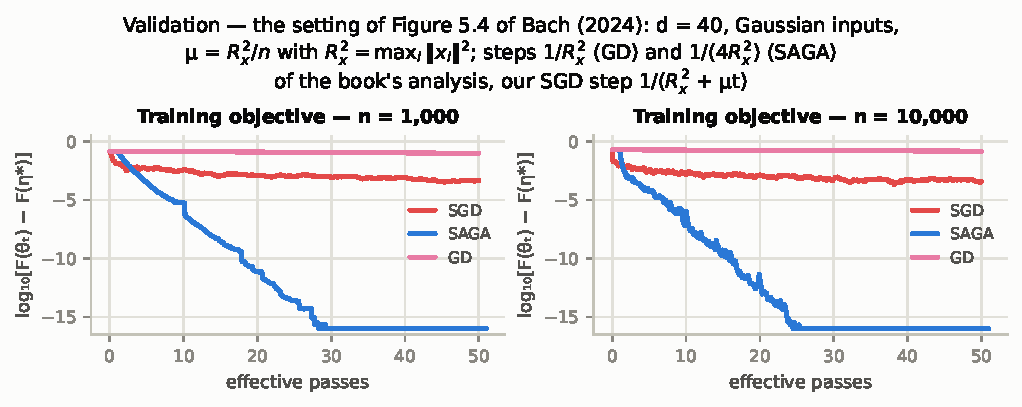
\includegraphics[width=\textwidth]{fig0_validation_book}
  \caption{\textbf{Validation on the setting of Figure~5.4 of~\cite{bach2024learning}.} $\ell_2$-regularized logistic
  regression with $d=40$ standard Gaussian features, $y=\mathrm{sign}(x^\top w+\text{noise})$, $\lambda=\mu=R_x^2/n$ with
  the book's constant $R_x^2=\max_i\norm{x_i}^2$, the steps of the book's analysis, GD $1/R_x^2$ and SAGA $1/(4R_x^2)$, and
  our SGD step $1/(R_x^2+\mu t)$. Training objective $F(\theta_t)-F(\etastar)$ against effective passes for $n=1{,}000$
  (left) and $n=10{,}000$ (right), one run each. SAGA reaches $10^{-8}$ after $13.6$ and $11.4$ passes and the floor of
  double precision ($\approx10^{-16}$) in fewer than 30 passes.}
  \label{fig:validation}
\end{figure}

% -----------------------------------------------------------------------------------------------------
% B3. Sources: digest.md (B3 tables), results/B3_summary.json (speed-ups, shares in orders A and B, late window,
% ratios, mu_eff_geomean, seed spread of the shares), findings.md Sec. 1. Product of the measured factors (I1--I2
% factor times mu_eff/mu) computed from the window geometric means of B3_summary.json; product of exact contractions
% versus realized V_t (seed 0) computed from results/B3.pkl with vrlab.analysis.trajectory_bounds (cut at V < 1e-18;
% ratio to V_t at the cut 5.17 and 3.41 for kappa = 1e2, 1e3, and between 0.129 and 5.52 all along, i.e. at most a
% factor 7.75; 0.955 and 0.959 after 100 passes for kappa = 1e4, 1e5; kappa = 10: V_t over the product 11 after 20
% passes, 24.1 to 1.18e3 beyond 30 passes, at most 3.07 of 19.3 decades; rho_exact(0) = 0.98616 held for n/10
% iterations gives 0.248 against V_{n/10}/V_0 = 0.691, i.e. a product of 0.359 V_t at t = n/10, 2.77-2.79 times below
% V_t on the five seeds).
% -----------------------------------------------------------------------------------------------------
\subsection{Where the proof of Proposition~5.9 loses (hypothesis B3)}\label{sec:exp-B3}

\paragraph{Question and measurements.}
Which inequalities make $\rho_{\rm bound}=1-\min\{\frac1{3n},\frac{3\mu}{16R^2}\}$ pessimistic, and how does this depend
on the conditioning and the anisotropy of the data? We run SAGA with the textbook constants ($\gamma=1/(4R^2)$,
$\Delta=3\gamma^2$) on the fifteen problems $\kappa\in\{10,\dots,10^5\}$, $\alpha\in\{0,1,2\}$, and record, with the
instruments of Section~\ref{sec:th-B3}, $\rho_{\rm exact}(t)$, the tightness ratios
$r_{\rm sq},r_{\rm coco},r_{\rm var},r_{\rm sc},r_{\rm min}$ of I1--I5 and $r_{\rm init}$ of I6, and the attribution chains of
\resref{prop:B3-attribution}, which undo the inequalities one at a time and split the logarithmic gap
$\log(1/\rho_{\rm exact})-\log(1/\rho_{\rm bound})$ into nonnegative \emph{shares}. Order~B (undo I5, I4, I2, I3, I1,
i.e.\ the intermediate rates of the proof applied cumulatively) is shown in the figures; order~A (I4, I2, I3, I1, then
I5) keeps the minimum until the end. Numbers are averages over passes 2--20 and over the 5 seeds unless stated
otherwise.

\paragraph{Size of the gap (Figure~\ref{fig:fig1}).}
The speed-up is $3.2$--$3.7$ for $\kappa\le10^2$, where the memory term $\frac1{3n}$ is the active one, and grows with
$\kappa$ in the parameter-term regime: $5.1$, $5.2$ and $3.4$ at $\kappa=10^3$, $29$, $16$ and $6.0$ at $\kappa=10^4$, $220$,
$100$ and $19$ at $\kappa=10^5$, for $\alpha=0$, $1$ and $2$ (passes 20--100: $187$, $72$ and $11$ at $\kappa=10^5$). At
$\kappa=10^4$ and $\alpha=1$, the mean squared distance decreases from $\norm{\theta_0-\etastar}^2=1954$ to $7.1\cdot10^{-9}$
in 100 passes, by $11.4$ orders of magnitude, whereas the bound only decreases by the factor $\rho_{\rm bound}^{10^5}=0.15$,
to $29\norm{\theta_0-\etastar}^2$ with the constant $1+\frac{3n}{16}$ of the proof ($38\norm{\theta_0-\etastar}^2$ with the
$1+\frac n4$ of the statement). Along seed $0$ ($\alpha=1$), the product of the exact conditional contractions agrees
with the realized $V_t$ within $5\%$ after 100 passes at $\kappa=10^4$ and $10^5$ ($11.5$ and $6.5$ decades of decrease),
and within a factor $5.2$ where the curves reach the floor at $\kappa=10^2$ and $10^3$ (about 20 decades; within a factor
$7.8$ all along). At $\kappa=10$ (not shown in Figure~\ref{fig:fig1}) the realized $V_t$, then carried by its memory
term, stalls for several passes before
dropping abruptly, and the two differ by a factor $11$ after 20 passes and by $24$ to $1.2\cdot10^3$ beyond 30 passes,
i.e.\ by up to three of 19 decades (a factor of about $2.8$ comes from holding the contraction of the fresh memory at
$t=0$ for $n/10$ iterations: the product is already $0.36\,V_t$ at $t=n/10$). The exact one-step identity thus accounts
for the observed decay, and the gap lies
essentially in the inequalities.

\begin{figure}[tbp]
  \renewcommand{\thefigure}{1}% project figure name (see the header of this file)
  \centering
  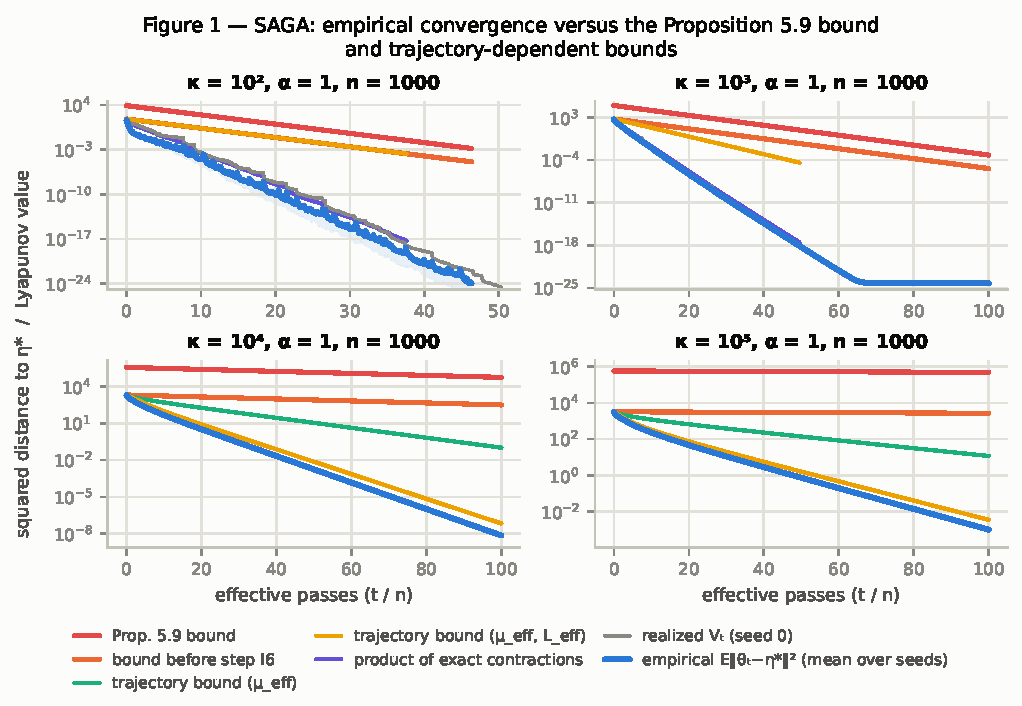
\includegraphics[width=\textwidth]{fig1_convergence_vs_bound}
  \caption{\textbf{Figure~1 of the proposal: SAGA against the bound of Proposition~\ref{prop:59}.} Logistic regression,
  $n=1{,}000$, $d=50$, $\alpha=1$, $\kappa\in\{10^2,10^3,10^4,10^5\}$ (one panel each), step $\gamma=1/(4R^2)$. Blue:
  $\E\norm{\theta_t-\etastar}^2$ estimated by the mean over 5 seeds (band: min--max); red: the bound of
  Proposition~\ref{prop:59} with the constant $1+3n/16$ obtained in its proof (the statement rounds it up to
  $1+n/4$); orange: the same bound before the initialization step I6, $\rho_{\rm bound}^tV_0$ ($V_t$ is the Lyapunov
  function of Section~\ref{sec:setting}); green and yellow: products, along the realized trajectory of seed $0$ and from its
  $V_0$, of the factors of \protect\resref{prop:B3-traj}, with $\mu$ replaced by $\muEff(\theta_{t-1})$ (green)
  and, in addition, $R^2$ replaced by $\LEff(\theta_{t-1})$ in the coefficient of the parameter term (yellow); violet:
  product of the exact conditional contractions $\rho_{\rm exact}(t)$ along the same trajectory; grey: realized Lyapunov
  value $V_t$ of seed $0$. The factors are computed every $n/10$ iterations and held constant in between. The three
  trajectory-dependent products (green, yellow, violet) are cut at the first instrumentation time with $V_t<10^{-18}$,
  below which the conditional expectations are dominated by rounding; the other curves end with the runs, which stop at
  $\norm{\theta_t-\etastar}^2\le10^{-26}$ (the mean and the two bounds with the shortest of the five). Where the memory
  term $1/(3n)$ is the active one in the a-posteriori factors ($\kappa\le10^3$ here, since $\muEff/\mu\ge16\kappa/(9n)$ along
  these runs; in the certified factor only for $\kappa\le10^2$, as $\frac3{16\kappa}<\frac1{3n}$ for $\kappa>\frac{9n}{16}$) the
  green and yellow curves coincide, and for $\kappa=10^2$ they also coincide with the orange one; for $\kappa\ge10^4$ the
  violet and grey curves are indistinguishable from the blue one and hidden under it. One legend, below the panels,
  serves all of them.}
  \label{fig:fig1}
\end{figure}

\paragraph{Tightness ratios (Figure~\ref{fig:fig2}).}
I3 and I5 are nearly tight on all fifteen problems: $r_{\rm var}\ge0.958$, because the mean stored error $\bar z$ is small
compared with the individual ones ($r_{\rm var}=1-n\norm{\bar z}^2/M$), and $r_{\rm min}\ge0.9998$. The square-norm step has
$r_{\rm sq}=0.50$--$0.52$ for $\kappa\le10^2$, the factor $2$ lost, by item~(iii) of \resref{lem:B3-ranges}, when the
gradient changes $a_i$ and the memory errors $b_i$ (the values of $a_t$ and $b_t$ of I1 when $i(t)=i$) are uncorrelated,
and $0.075$, $0.015$ and $0.0035$ at $\kappa=10^5$, where the memory is fresh relative to the slow motion of $\theta_t$, as
\resref{rem:B3-fresh} explains. Cocoercivity has $r_{\rm coco}=\LEff/R^2$ in
$[0.16,0.37]$, $[0.11,0.16]$ and $[0.019,0.18]$ for $\alpha=0,1,2$: $R^2=\max_iL_i$ overestimates the constant met along the
trajectories by a factor $2.7$ to $52$. Strong convexity has $r_{\rm sc}=\mu/\muEff$ between $0.74$ and $0.90$ at $\kappa=10$
and $0.012$, $0.027$ and $0.14$ at $\kappa=10^5$, i.e.\ $\muEff/\mu=81$, $37$ and $6.9$ against
$\lmin(F''(\etastar))/\mu=70$, $26$ and $2.1$ (the iterates are still far from $\etastar$ during passes 2--20). Finally
$r_{\rm init}$ is $3.1\cdot10^{-5}$ to $0.028$, but I6 only enters the constant $1+\frac n4$.

\begin{figure}[tbp]
  \renewcommand{\thefigure}{2}% project figure name (see the header of this file)
  \centering
  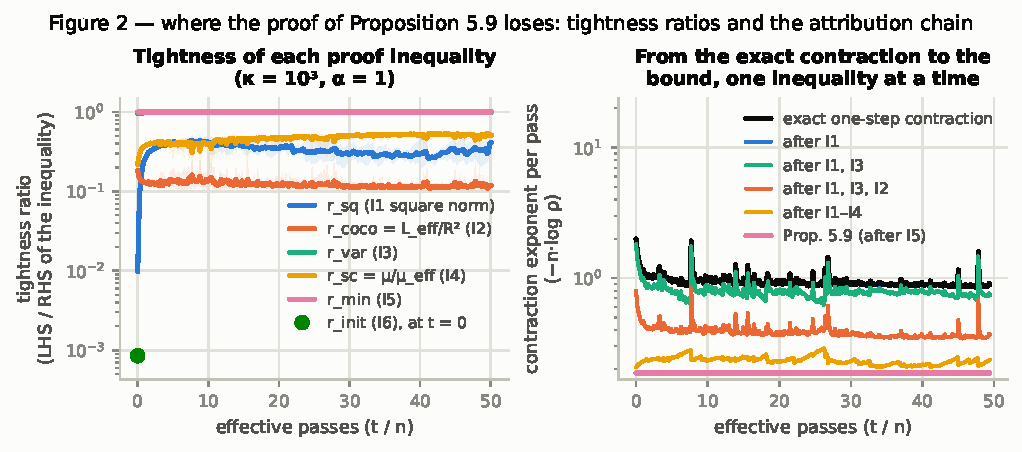
\includegraphics[width=\textwidth]{fig2_tightness_ratios}
  \caption{\textbf{Figure~2 of the proposal: tightness of each inequality of the proof.} Logistic regression,
  $n=1{,}000$, $d=50$, $\kappa=10^3$, $\alpha=1$, textbook constants. Left: tightness ratios of I1--I5
  (\protect\resref*{def:B3-ratios}: smaller side over larger side, $1$ meaning equality), computed from exact conditional
  expectations every $n/10$ iterations; geometric mean over 5 seeds (band: min--max), records with $V_t<10^{-18}$
  discarded. The ratio of the initialization inequality I6, $r_{\rm init}=8.5\cdot10^{-4}$ for this problem, is the single
  marker at $t=0$, below the other curves. Right: attribution chain along seed $0$ (order~B of
  \protect\resref*{prop:B3-attribution}, records with $V_t\ge10^{-18}$): contraction exponent per pass, $-n\log\rho$, of the
  exact one-step contraction and after applying the inequalities cumulatively in the order of the proof (I1, I3, I2,
  I4, I5), down to the certified rate of Proposition~\ref{prop:59}. The curve after I1 is hidden under the curve after
  I1 and I3, because I3 is nearly tight.}
  \label{fig:fig2}
\end{figure}

\paragraph{Attribution (Figure~\ref{fig:fig3}).}
In order~B, for $\kappa\le10^2$ the gap is carried by I1 ($0.39$--$0.44$) and I2 ($0.32$--$0.37$), then I5 ($0.07$--$0.22$)
and I4 ($0.03$--$0.17$). For $\kappa\ge10^4$, cocoercivity dominates ($0.46$ for $\alpha=0$, $0.54$--$0.58$ for $\alpha=1$,
$0.62$--$0.71$ for $\alpha=2$), strong convexity follows ($0.25$--$0.36$), and together they carry $0.77$--$0.96$ of the
gap, while I1 falls to $0.03$--$0.16$ and I5 to at most $0.073$; at $\kappa=10^3$ and $\alpha=2$, I2 alone carries $0.83$.
Over the grid the largest share of I3 is $0.54\%$ and that of I5 is $22\%$ (a ratio as close to $1$ as $r_{\rm min}$
still matters because the exponents are small: at $\kappa=10$, I5 adds about $2\cdot10^{-4}$ per iteration to a certified
exponent of $3.3\cdot10^{-4}$); the seed-to-seed spread of the shares is below $0.03$ for $\kappa\ge10^4$. Order~A also
gives I3 a small share (at most $0.006$, except $0.063$ at $\kappa=10^3$, $\alpha=2$) and gives $0.59$--$0.96$ to I4 and I2 together
for $\kappa\ge10^4$, but for $\kappa\le10^2$ it gives $0.56$--$0.61$ to the minimum I5, $0.38$--$0.44$ to I1 and nothing to
I4 and I2, which only lower the parameter coefficient, not the active one there: as \resref{rem:B3-orders} explains, the
attribution is order dependent where the two components of $V_t$ compete.

\begin{figure}[tbp]
  \renewcommand{\thefigure}{3}% project figure name (see the header of this file)
  \centering
  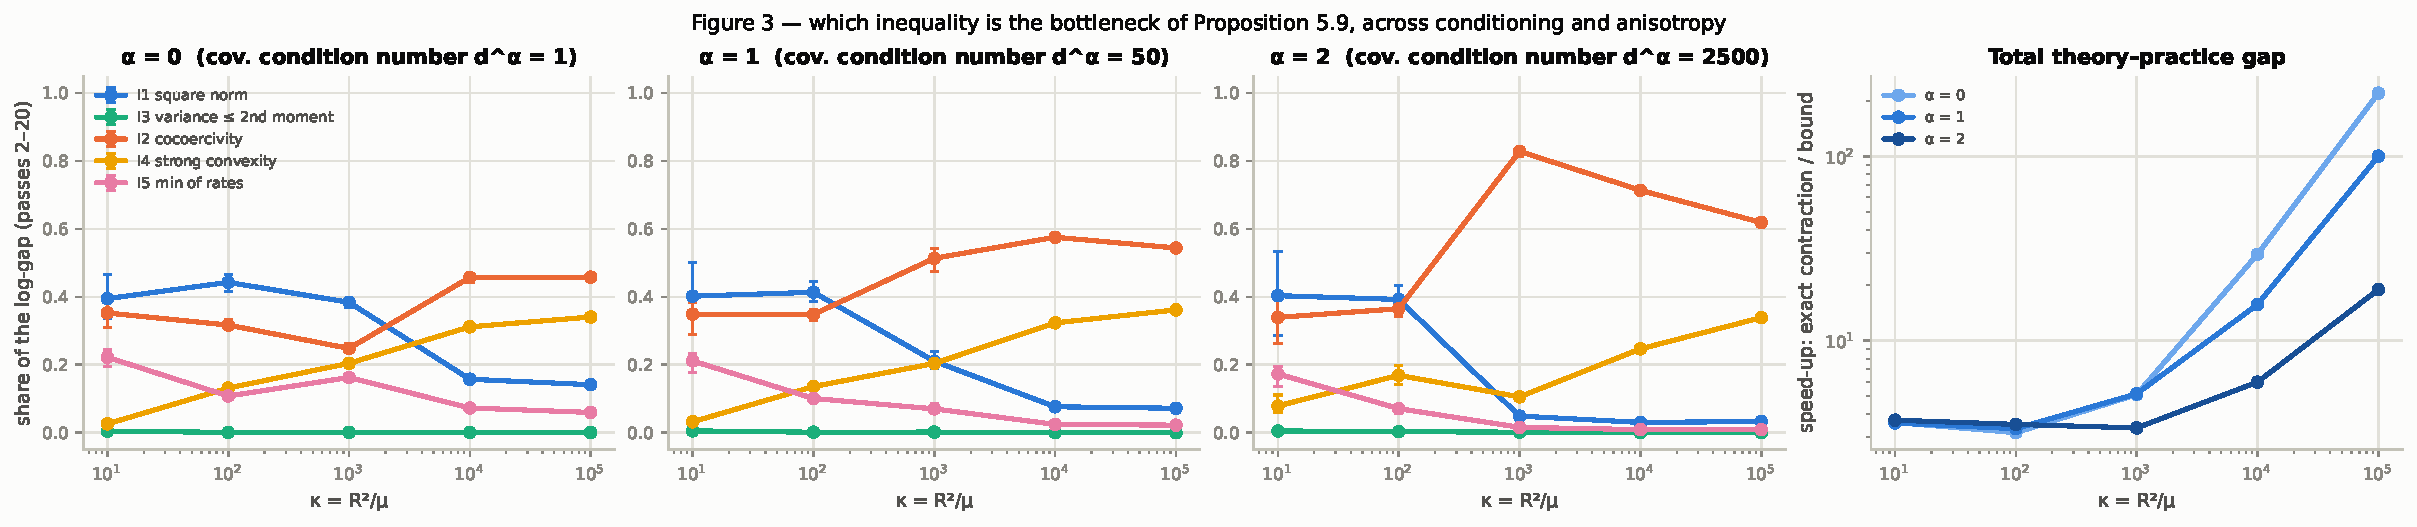
\includegraphics[width=\textwidth]{fig3_bottleneck_by_geometry}
  \caption{\textbf{Figure~3 of the proposal: which inequality is the bottleneck.} Share of the logarithmic gap between the
  exact one-step contraction and the certified one attributed to each inequality (order~B of
  \protect\resref*{prop:B3-attribution}, i.e.\ cumulative attribution in proof order), averaged over passes 2--20
  (records with $V_t\ge10^{-18}$) and over 5 seeds (error bars: min--max over seeds), as a function of $\kappa$, for the
  covariance spectra $j^{-\alpha}$, $\alpha\in\{0,1,2\}$ (top left, top right and bottom left; population condition numbers
  $1$, $50$, $2500$); logistic regression, $n=1{,}000$, $d=50$, textbook constants. Bottom right: total speed-up factor
  $(-\log\rho_{\rm exact})/(-\log\rho_{\rm bound})$ (window average, mean over seeds).}
  \label{fig:fig3}
\end{figure}

\paragraph{Interpretation.}
By \resref{prop:B3-representation} the exact parameter coefficient is
$1-\frac{\muEff}{2R^2}\big(1-r_{\rm coco}(\frac{r_{\rm sq}}4+\frac38)\big)$: relative to the worst case, I4 multiplies the
parameter exponent by $\muEff/\mu\in[1,\kappa]$ (item~(i) of \resref*{lem:B3-ranges}), and I1 and I2 together by
$\big(1-r_{\rm coco}(\frac{r_{\rm sq}}4+\frac38)\big)/\frac38\in[1,\frac83]$ at the fixed step
(\resref*{rem:B3-fixed-step}). For $\kappa\ge10^4$, where the parameter term is active and $D_t$ carries most of $V_t$
($r_{\rm min}\approx1$), inserting the window geometric means of the ratios into this product reproduces $0.91$--$0.96$ of
the measured speed-ups: $\muEff/\mu$ (between $2.2$ and $81$) times a factor $2.45$--$2.62$ from I1 and I2. The
$\kappa$-dependent part of the gap is thus the strong-convexity step, the difference between $\mu=\lambda$ and the
curvature met along the trajectory; cocoercivity contributes a bounded factor, whose larger additive share in order~B
comes from acting on an exponent already multiplied by $\muEff/\mu$. With strongly anisotropic features ($\alpha=2$) the
bottom of the spectrum of $F''(\etastar)$ stays close to $\lambda$, so I4 is closer to tight and I2 dominates the shares.
The large factors at $\kappa=10^5$ are a property of these instances, not of the order of the bound: by
\resref{prop:B3-lower} no analysis of SAGA with a constant step can improve the exponent $1$ of $\kappa$
uniformly over the class of Proposition~\ref{prop:59} (caveat~(ii) of \resref*{rem:B3-conclusion}).

% -----------------------------------------------------------------------------------------------------
% Constants. Sources: results/GammaDelta_summary.json, digest.md "(gamma, Delta) inside the proof", per-seed rates
% in results/GammaDelta.pkl (all three seeds converge at every step); B3 note Prop. B3-optimum, Cor. B3-c.
% kappa <= 1e2 (findings.md Sec. 4; B3 note, paragraph "Comparison with the textbook choice", Remark rem:B3-conclusion
% and Outcome): at gamma = 1/(4R^2) the best c is c_Delta = (6s-16+sqrt((6s-16)^2+128s))/(2s), s = n/kappa, = 5.036 and
% 5.894, with rate (6-c)/(16 kappa) = 1.8085 and 1.9821 times 1/(3n); Q(10) = 2.4223, Q(100) = 2.9400; speed-ups of
% B3_summary.json divided by these: 1.754--1.945 and 1.217--1.452; c_exact_per_iter / (-log(1-1/n)) = 1.057--1.236.
% -----------------------------------------------------------------------------------------------------
\subsection{The constants of the proof}\label{sec:exp-constants}

Is the gap a matter of the convenient constants $\gamma=1/(4R^2)$ and $\Delta=3\gamma^2$? \resref{prop:B3-optimum} gives
the best pair $(\gamma,\Delta)$ in closed form; by \resref{rem:B3-conclusion}, it improves the certified rate by a factor
between $1.05$ and $3$, and by at most $\frac43$ when $\kappa\ge9n/16$. At $\kappa=10^3$ the
optimum is $\gamma R^2=0.219$, $\Delta=2.56\gamma^2$, with certified rate $2.19\cdot10^{-4}$ per iteration against
$1.875\cdot10^{-4}$, a gain of $17\%$. On logistic regression ($\kappa=10^3$, $\alpha=1$, 3 seeds, slopes over passes 2--40,
Figure~\ref{fig:C}) the observed exponent per pass is $0.51$, $0.97$, $1.14$, $1.09$, $0.95$, $0.66$ and $0.027$ for
$\gamma R^2=\frac18$, $\frac14$, $\frac13$, $\frac12$, $1$, $2$ and $4$, whereas the best certificate is $0.18$, $0.22$ and $0.17$
for the first three steps and does not exist for $\gamma R^2\ge\frac12$, where, by \resref{cor:B3-c}, no $\Delta$ is
admissible. At the textbook step the observed exponent is $4.5$ times the best certificate, and SAGA,
fastest around $\gamma R^2=\frac13$, still converges for all three seeds at $\gamma R^2=4$, eight times the supremum
$\frac12$ of the steps $\gamma R^2$ that the proof admits. The constants of Proposition~\ref{prop:59} are thus within $17\%$
of the best ones of their proof at this conditioning, and the factor $4.5$ left at the textbook step is the slack of the
inequalities (\resref*{rem:B3-conclusion}); the admissible range $\gamma R^2<\frac12$ itself comes from absorbing the
second moment $\gamma^2\Omega_{t-1}$ of the step and the memory refresh with the worst-case bounds I1--I3.

These conclusions concern $\kappa=10^3\ge\frac{9n}{16}$, where the textbook rate is the parameter term and the constants
can gain at most $\frac43$. For $\kappa\le10^2$, where it is the memory term $\frac1{3n}$, the constants account for a
larger part of the speed-ups $3.2$--$3.7$ of Section~\ref{sec:exp-B3}: at the textbook step, the best weight,
$\Delta=c\gamma^2$ with $c\approx5.04$ ($\kappa=10^2$) or $c\approx5.89$ ($\kappa=10$) instead of $c=3$, multiplies the
certified rate by $1.81$ or $1.98$, and the optimal constants of \resref*{prop:B3-optimum}, at a smaller step, by $2.42$
or $2.94$, leaving factors $1.75$--$1.95$ and $1.22$--$1.45$, respectively. The exact exponents $-\log\rho_{\rm exact}$
there (passes 2--20, mean over the seeds) are $1.06$--$1.24$ times $-\log(1-\frac1n)$, the largest exponent $-\log\rho$
of a bound $\E[V_t]\le c_0\rho^tV_0$ with $c_0$ independent of $t$, whatever $\Delta$ (\resref*{rem:B3-conclusion}): a
typical trajectory of $V_t$ decreases faster than its expectation can.

\begin{figure}[tbp]
  \renewcommand{\thefigure}{C}% project figure name (see the header of this file)
  \centering
  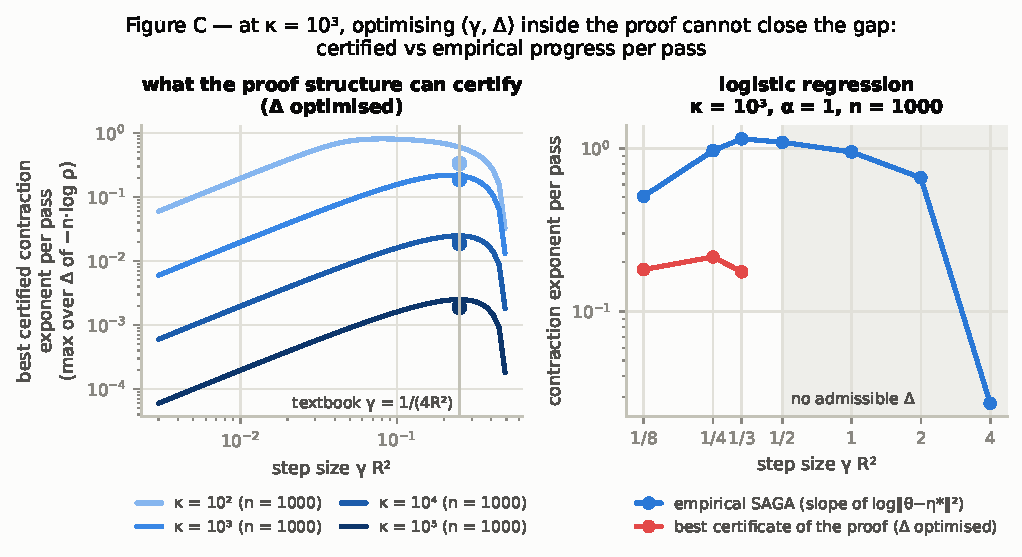
\includegraphics[width=\textwidth]{figC_gamma_delta}
  \caption{\textbf{The constants inside the proof.} Left: best contraction exponent per pass that the proof structure of
  Proposition~\ref{prop:59} can certify, as a function of the step $\gamma R^2$, with the Lyapunov weight $\Delta=c\gamma^2$
  optimized over $c$ (\protect\resref*{cor:B3-c}), for $\kappa\in\{10^2,10^3,10^4,10^5\}$ and $n=1{,}000$; dots: textbook
  constants $\gamma=1/(4R^2)$, $\Delta=3\gamma^2$. Right: logistic regression ($\kappa=10^3$, $\alpha=1$, $n=1{,}000$, $d=50$),
  empirical contraction exponent per pass of SAGA (least-squares slope of $\log\norm{\theta_t-\etastar}^2$ over passes
  2--40, mean over 3 seeds) and best certificate of the proof at the same step; the proof certifies nothing for
  $\gamma R^2\ge\frac12$, where no $\Delta$ is admissible (shaded region).}
  \label{fig:C}
\end{figure}

% -----------------------------------------------------------------------------------------------------
% B2. Sources: results/B2_summary.json and the B2 tables of digest.md (start, geometric-mean and end values, d_eff,
% quadratic proxy, monotone fractions, run ends, last-five-pass statistics saga_last5_*, GD end states, minima of
% mu_eff/mu over the kept and over all records, and the criterion 9 n lmin/(16 R^2) under the key crit_9n_lmin_over_16R2);
% GD monotonicity exceptions: keys gd_mu_eff_increasing_steps, gd_mu_eff_increase_max_rel and gd_D_max_after_increase
% (13 of 118 and 56 of 400 GD steps for alpha = 0, kappa = 1e3, 1e4; computed from results/B2.pkl); B2 note
% Rem. B2-P2-outcome, findings.md Sec. 2; order-A shares from B3_summary.json (key shares_orderA); lmin(F''(eta*))/mu
% up to 69.9 over the fifteen B3 problems (B3_summary.json, key mu_local_over_mu). States with mu_eff < mu: only ten
% discarded GD states, for alpha = 2, kappa = 1e2 (iterations 240-249, ||theta_t - eta*||^2 from 6.9e-26 to 9.8e-27,
% mu_eff/mu from 0.993 down to 0.795), computed from results/B2.pkl (the summary stores the minimum under the key
% gd_mu_eff_over_mu_min_all_states).
% -----------------------------------------------------------------------------------------------------
\subsection{Effective curvature along the trajectories (hypothesis B2)}\label{sec:exp-B2}

Are the constants $\muEff(\theta_t)$ and $\LEff(\theta_t)$ of \resref{def:B2-eff}, which make I4 and I2 identities
at the current iterate, much better than $\mu$ and $R^2$, and do they explain the gap (Section~\ref{sec:th-B2})? Along one
SAGA run and one GD run per problem ($\kappa\in\{10^2,10^3,10^4\}$, $\alpha\in\{0,1,2\}$) we record $\muEff/\mu$, $\LEff/R^2$,
the share $\pi_{\min}(t)$ of $\norm{\theta_t-\etastar}^2$ carried by the eigenvector $q_{\min}$ of $F''(\etastar)$ with the
smallest eigenvalue, and the effective number of directions $d_{\rm eff}(t)=1/\sum_k\pi_k(t)^2$ of the error in the
eigenbasis of $F''(\etastar)$, not to be confused with the ridge effective dimension $d_{\rm eff}(\lambda)$ of
Section~\ref{sec:th-B1} (Figure~\ref{fig:B2}).

\begin{figure}[tbp]
  \renewcommand{\thefigure}{B2}% project figure name (see the header of this file)
  \centering
  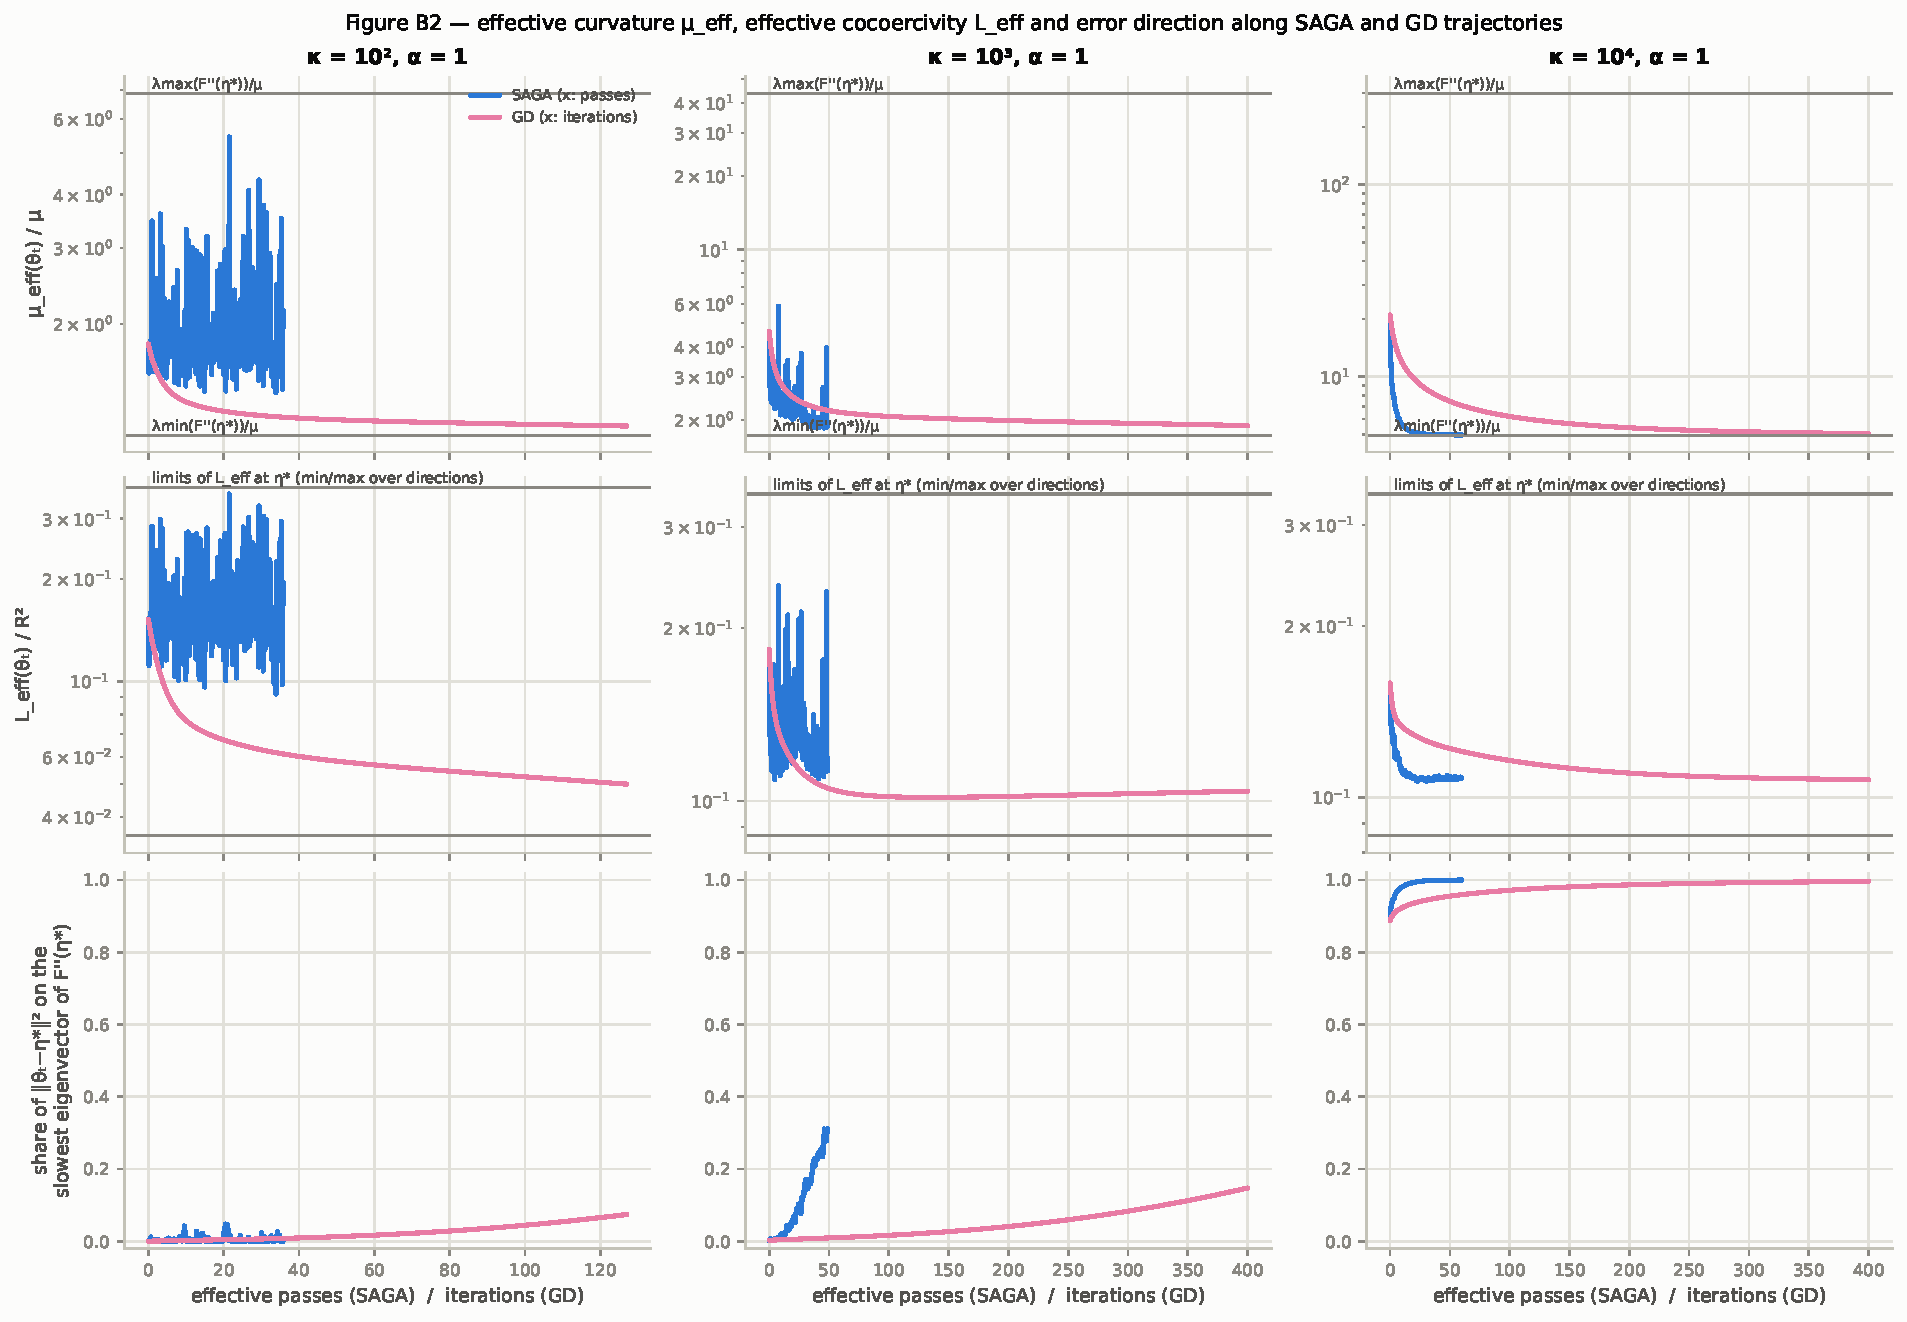
\includegraphics[width=\textwidth]{figB2_effective_curvature}
  \caption{\textbf{Hypothesis B2: effective constants along the trajectories.} $\muEff(\theta_t)/\mu$ (top),
  $\LEff(\theta_t)/R^2$ (middle) and share $\pi_{\min}$ of $\norm{\theta_t-\etastar}^2$ carried by the eigenvector of
  $F''(\etastar)$ with the smallest eigenvalue (bottom), along SAGA (blue, $x$-axis in passes, $\gamma=1/(4R^2)$, at most 60
  passes) and gradient descent (magenta, $x$-axis in iterations, step $1/L_F$, at most 400 iterations), for
  $\kappa\in\{10^2,10^3,10^4\}$ (one column each), $\alpha=1$, $n=1{,}000$, $d=50$, one seed; states with
  $\norm{\theta_t-\etastar}^2<10^{-18}$ are discarded, so that the runs reaching this floor end earlier (SAGA after $36$ and
  $49$ passes for $\kappa=10^2$ and $10^3$, GD after $127$ iterations for $\kappa=10^2$). Horizontal lines:
  $\lmin(F''(\etastar))/\mu$ and $\lmax(F''(\etastar))/\mu$ (top), smallest and largest limits of $\LEff/R^2$ at $\etastar$
  over directions (middle). The configurations $\alpha\in\{0,2\}$ are summarized in Section~\ref{sec:exp-B2}.}
  \label{fig:B2}
\end{figure}

The bound $\muEff\ge\mu$ of \resref{lem:B2-mueff} holds at every retained state (ten discarded GD states below the floor,
at $\alpha=2$, $\kappa=10^2$, give $\muEff/\mu$ between $0.795$ and $0.993$, a rounding artefact), and along SAGA $\muEff/\mu$ starts between
$1.8$ and $50$. The SAGA runs end after 60 passes (last record at pass $59.9$), or after 34 to 49 passes for the five runs
that reach the floor ($\kappa\le10^3$, except $\alpha=2$, $\kappa=10^3$). For $\kappa=10^4$ and $\alpha\in\{0,1\}$ the
error of SAGA concentrates on $q_{\min}$ ($\pi_{\min}=0.998$ and $0.9996$ at the end, $d_{\rm eff}=1.005$ and $1.001$;
from $\theta_0=0$, $\pi_{\min}$ starts at $0.984$ and $0.888$, and for $\alpha=0$ it first drops to $0.938$ at pass
$3.1$), and $\muEff/\mu$ ends within $1\%$ of $\lmin(F''(\etastar))/\mu$ ($9.94$ against $9.86$, $4.97$ against $4.97$);
GD aligns with $q_{\min}$ as well ($\pi_{\min}=1.000$ and $0.996$ after 400 iterations), its $\muEff$ ending at
$\lmin(F''(\etastar))$ and $1.8\%$ above it. For $\kappa=10^2$ the error of SAGA does not concentrate ($\pi_{\min}\le0.05$
over the last five passes, $d_{\rm eff}$ about $18$ and $14$ on average for $\alpha=0,1$) and $\muEff/\mu$ fluctuates
above $\lmin(F''(\etastar))/\mu$ (for $\alpha=1$: geometric mean $1.90$ over the run, between $1.38$ and $3.63$ over the
last five passes, against $1.10$, while GD ends at $1.15$); at $\kappa=10^3$ the alignment is partial ($\alpha=1$:
$\pi_{\min}=0.31$) or absent ($\alpha=0$: $d_{\rm eff}$ about $17$ over the last five passes, while GD is aligned). For
$\alpha=2$ the bottom of the spectrum of $F''(\etastar)$ is nearly degenerate and neither method aligns with $q_{\min}$
(for $\kappa\ge10^3$, GD has moreover not converged after 400 iterations: $\norm{\theta_t-\etastar}^2=5.7\cdot10^{-4}$ and
$202$). Along GD, $\muEff$ is non-increasing at every step up to rounding, as it is exactly on a quadratic by
\resref{prop:B2-gd}: the exceptions, $13$ of $118$ and $56$ of $400$ steps for $\alpha=0$ and $\kappa=10^3$, $10^4$, are
relative increases of at most $7.2\cdot10^{-7}$ and $2.7\cdot10^{-6}$, at states with
$\norm{\theta_t-\etastar}^2\le8.3\cdot10^{-14}$ and $8.1\cdot10^{-13}$. At the end of every SAGA run the quadratic proxy
$\sum_k\lambda_k\pi_k(t)$, with $\lambda_k$ the eigenvalues of $F''(\etastar)$, matches $\muEff$ within $1\%$: near
$\etastar$, $\muEff$ is set by the direction of the error, as \resref{prop:B2-limits} states. The geometric means of
$\LEff/R^2$ along SAGA are $0.19$--$0.38$, $0.11$--$0.16$ and $0.012$--$0.09$ for $\alpha=0,1,2$.

The effective curvature thus exceeds $\mu$ by at least the factor $\lmin(F''(\etastar))/\mu$ near $\etastar$ (up to $9.9$
in these runs, and up to $70$ over the problems of Section~\ref{sec:exp-B3}) and by more far from it, and $\LEff$ is $2.6$
to $86$ times smaller than $R^2$, as hypothesis B2 states. Prediction (P2) of Section~\ref{sec:B2-direction}, that the
error of SAGA stays spread over the directions fed by its noise, holds in the four runs with
$9n\lmin(F''(\etastar))/(16R^2)>1$ ($\kappa=10^2$, and $\kappa=10^3$ with $\alpha=0$) and fails at $\kappa=10^4=10n$ for
$\alpha\in\{0,1\}$, where SAGA aligns with $q_{\min}$ like GD; the three other runs are intermediate (partial alignment at
$\kappa=10^3$, $\alpha=1$; for $\alpha=2$ and $\kappa\ge10^3$, a nearly degenerate bottom spectrum, and neither method
aligns with $q_{\min}$). In terms of $\kappa$ alone, (P2) thus holds only for $\kappa$ at most of the order of $n$, and not in every such
run: $\kappa\approx n$ does not suffice. \resref{rem:B2-P2-outcome} explains the alignment heuristically: when
$n\gamma\lmin(F''(\etastar))$ is small, the iterate moves little during one refresh cycle of the memory, so that the noise
decays with the slowest mode of the mean dynamics instead of at the certified rate (the noise spectrum was not recorded,
so this mechanism is inferred, not measured). For the bound, the one-step factors of \resref{prop:B3-traj} are exactly the
first two steps of order~A of \resref{prop:B3-attribution}: replacing $\mu$ by $\muEff(\theta_{t-1})$ recovers
$0.25$--$0.37$ of the logarithmic gap for $\kappa\ge10^4$ (green curves in Figure~\ref{fig:fig1}), and replacing in
addition $R^2$ by $\LEff(\theta_{t-1})$ in the parameter coefficient recovers $0.59$--$0.96$ (yellow), whereas for
$\kappa\le10^2$ they recover nothing: the bound is then saturated by the memory term, as explained in
\resref{rem:B2-what-explains}. These are a-posteriori statements; the a-priori version, \resref{prop:B3-region}, was not
evaluated along the runs (Section~\ref{sec:th-B3} only computes the rate it gives on a ball around $\etastar$).

% -----------------------------------------------------------------------------------------------------
% B1. Sources: digest.md B1 table, results/B1_summary.json, B1 note (Props. B1-transfer, B1-nofreelunch, B1-diag,
% Rem. B1-memory-bottleneck, predictions (P1)--(P3) and their outcome paragraph), findings.md Sec. 3. Split of the factor
% 3.3-3.8 along order A (memory coefficient 1.95-1.99, I5 1.55-1.70, pathwise remainder 1.10-1.12) and the factor
% 1.10-1.26 invisible in E V_t^P: B1 note, Outcome, and findings.md Sec. 3 (computed from results/B1.pkl).
% -----------------------------------------------------------------------------------------------------
\subsection{SAGA in a fixed quadratic metric (hypothesis B1)}\label{sec:exp-B1}

Does SAGA in the metric of a fixed positive definite $P$, $\theta_t=\theta_{t-1}-\gamma P^{-1}\omega_t$, converge faster,
and which steps of the proof change? By \resref{prop:B1-transfer}, the proof transfers with the relative constants
$(R_P^2,\mu_P)$, which gives \resref{cor:B1-rate}; for logistic regression, no $P$ improves the global condition number:
$\kappaP\ge\kappa$ by \resref{prop:B1-nofreelunch}, restated in Section~\ref{sec:th-B1}. We compare $P=I$, the Jacobi
metric $P_{\rm J}=\diag(\hat\Sigma)+\lambda I$, the statistical metric $\hat\Sigma+\lambda I$ and the Hessian
$F''(\etastar)$, with $\gamma=1/(4R_P^2)$, at $\kappa=10^3$ (Figure~\ref{fig:B1}); here and in the constants below,
$R_P^2$ is the upper bound $\frac14\max_i\norm{x_i}_{P^{-1}}^2+\lambda/\lmin(P)$ of~\eqref{eq:B1-logistic-RP}, exact for
$P=I$ and at most $5.2\%$ above the supremum of \resref{def:B1-kappaP} otherwise. In this order, the exponents per pass of
$\norm{\theta_t-\etastar}_P^2$ (passes 2--20) are $1.00$, $0.94$, $1.11$, $1.11$ for $\alpha=1$ and $0.61$, $0.27$,
$1.26$, $1.24$ for $\alpha=2$. The global constants favour $P=I$ instead: $\kappaP=1000$, $1899$, $5083$, $3623$
($\alpha=1$) and $1000$, $2852$, $3639$, $2089$ ($\alpha=2$) (with the exact supremum, $1000$, $1898$, $5057$, $3611$ and
$1000$, $2841$, $3459$, $2051$), and the certified exponents for $\alpha=1$ are $0.19$, $0.099$, $0.037$, $0.052$. With
the local constant $\lmin(F''(\etastar),P)$ (smallest generalized eigenvalue) in place of $\mu_P$, a heuristic
substitution that \resref{lem:B1-asymptotic} supports only as $\theta\to\etastar$, the relative condition numbers
$R_P^2/\lmin(F''(\etastar),P)$ become $576$, $641$, $166$, $83$ ($\alpha=1$) and $981$, $2433$, $103$, $41$ ($\alpha=2$)
(the condition numbers $\lmax/\lmin$ of $F''(\etastar)$ relative to $P$ are $25$, $26$, $2.8$, $1$ and $50$, $116$, $8.4$,
$1$), and Proposition~\ref{prop:59} so evaluated gives $0.33$, $0.29$, $0.33$, $0.33$ and $0.19$, $0.077$, $0.33$, $0.33$
per pass: the observed ordering, up to the near tie of the dense metrics, which saturate the memory term ($\frac13$ per
pass) while their observed exponents are $3.3$--$3.8$ times larger. In the $P$-geometry the slack moves from cocoercivity
to strong convexity: for $\alpha=1$, $r_{\rm coco}$ rises from $0.13$ to $0.33$--$0.34$ and $r_{\rm sc}$, computed with
the global $\mu_P$, falls from $0.42$ to $0.017$--$0.023$, as prediction (P2) of Section~\ref{sec:B1-predictions} anticipates.

\begin{figure}[tbp]
  \renewcommand{\thefigure}{B1}% project figure name (see the header of this file)
  \centering
  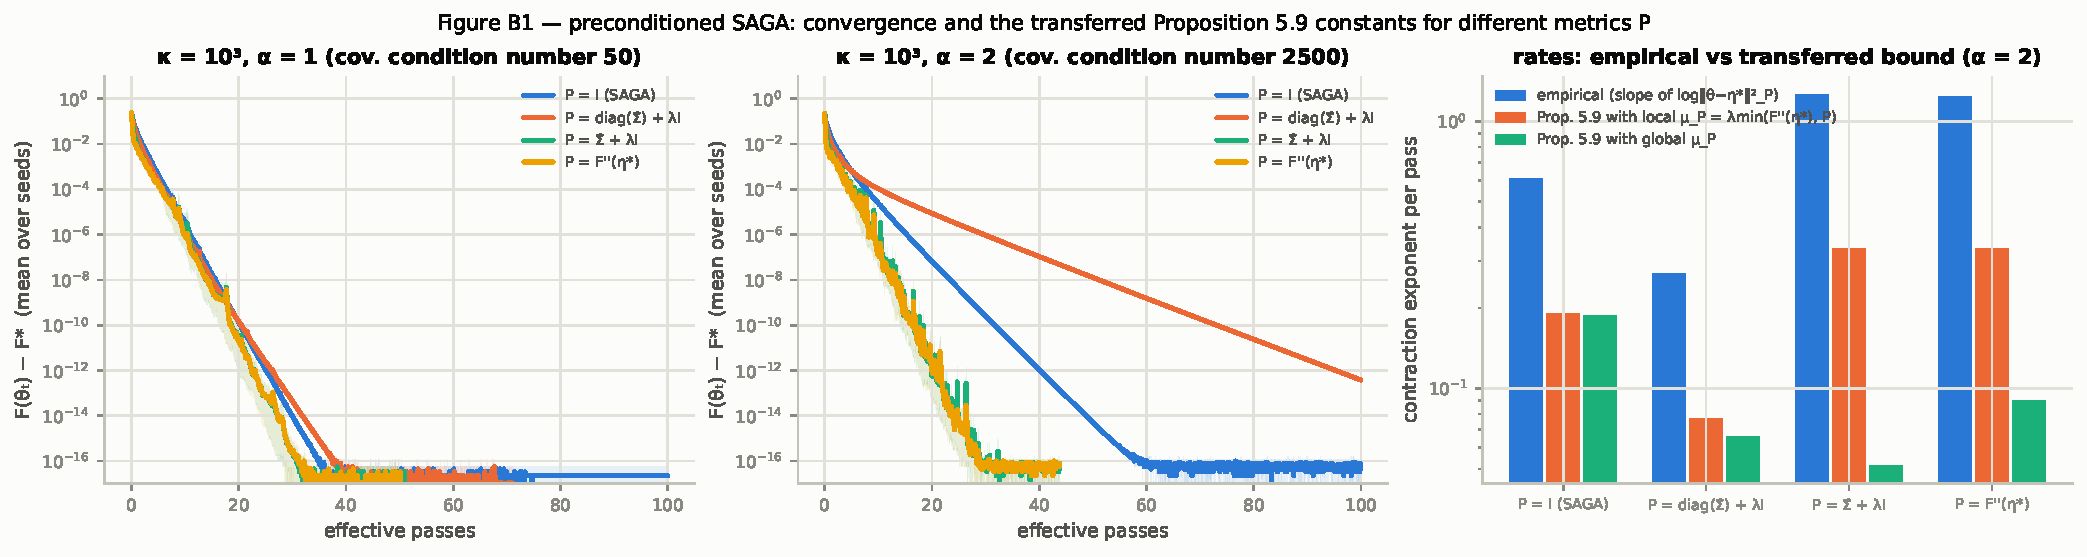
\includegraphics[width=\textwidth]{figB1_preconditioned_saga}
  \caption{\textbf{Hypothesis B1: SAGA in a fixed quadratic metric.} $\theta_t=\theta_{t-1}-\gamma P^{-1}\omega_t$ with
  $\gamma=1/(4R_P^2)$, where $R_P^2=\frac14\max_i\norm{x_i}_{P^{-1}}^2+\lambda/\lmin(P)$ is the upper
  bound~\eqref{eq:B1-logistic-RP} on the transferred smoothness constant, for
  $P\in\{I,\diag(\hat\Sigma)+\lambda I,\hat\Sigma+\lambda I,F''(\etastar)\}$, $\hat\Sigma=\frac1n\sum_ix_ix_i^\top$, on logistic
  regression ($n=1{,}000$, $d=50$, $\kappa=10^3$). Top: $F(\theta_t)-F(\etastar)$ for $\alpha=1$ (left) and $\alpha=2$ (right),
  mean over 5 seeds (band: min--max), up to the end of the shortest run (the runs stop at
  $\norm{\theta_t-\etastar}_P^2\le10^{-26}$). Bottom ($\alpha=2$): contraction exponent per pass of $\norm{\theta_t-\etastar}_P^2$
  (least-squares slope over passes 2--20, mean over seeds) against Proposition~\ref{prop:59} evaluated, heuristically, with
  the local constant $\lmin(F''(\etastar),P)$ (smallest generalized eigenvalue) and with the global constant $\mu_P$.}
  \label{fig:B1}
\end{figure}

The gain of a fixed metric is therefore real but entirely trajectory-dependent: invisible in the global constants, which
cannot improve for logistic regression, it appears in the local ones. Once the curvature is handled by $P$, the bound is
saturated by its memory term, the regime of \resref{rem:B1-memory-bottleneck}, $3.3$ to $3.8$ times below the observed
exponents. Along the measured trajectories (passes 2--20, in the $P$-geometry), this factor splits in three when the
inequalities are undone in order~A of \resref{prop:B3-attribution}, that is, I4, I2, I3, I1, then the min step I5. The memory
coefficient $1-\frac1{3n}$ comes from the textbook weight $\Delta=3\gamma^2$, which absorbs the memory term created by I1
and I3; evaluated exactly by \resref{prop:B3-representation}, with the measured $r_{\rm sq}\approx0.51$--$0.53$ and
$r_{\rm var}\approx1$, it is $1-\frac1n(1-\frac23r_{\rm sq}r_{\rm var})\approx1-\frac{0.65}n$: a factor $1.95$--$1.99$.
The min step I5 charges at the memory rate the parameter part of $V_t^P$, which contracts $7$ to $21$ times faster: a
factor $1.55$--$1.70$. The remaining factor, $1.10$--$1.12$, separates the measured slopes from the exact one-step
contraction. None of this concerns $\E V_t^P$: by the memory recursion~\eqref{eq:B3-EM}, the memory part of $\E V_t^P$
cannot decrease faster than $(1-\frac1n)^t$, so that no bound on $\E V_t^P$ certifies more than about $1$ per pass, $3$
times the local bound, and a factor $1.10$--$1.26$ of the observed exponents is invisible in the expectation that the
analysis controls. The Jacobi metric does not help, and is the slowest for both values of $\alpha$: the features are
randomly rotated, so the diagonal of $\hat\Sigma$ carries little of its anisotropy, and \resref{prop:B1-diag} only places
$P_{\rm J}$ within a factor $\operatorname{cond}(C_{\rm corr})$ of $\hat\Sigma+\lambda I$, in either direction: nothing in
the theory orders $P_{\rm J}$ with respect to $P=I$. The dense metrics cost $O(nd^2)$ per pass, and $P=F''(\etastar)$
requires $\etastar$ (an oracle benchmark).

% -----------------------------------------------------------------------------------------------------
% A3. Sources: results/A3_summary.json (rho_lemma; speed-ups speedup_exact_over_lemma and speedup_exact_over_rho, with
% rho = min{sigma/(6 theta_1), theta_1/(2n)}; r_var, r_cen, r_coco_lk, c_share, q_cancel, maximal violation; sign-aware
% keys contraction_componentwise_max, q_plus_frac_ge_1, q_cancel_frac_ge_1_given_inner_positive,
% c_share_frac_negative_given_q_ge_1), digest.md A3 tables, A3 note (Thm. lk, Lemma L1, Prop. cancel, eq. cancel,
% predictions (P2)-(P4), outcome paragraph), findings.md Secs. 5 and 8. B3 speed-ups on the same logistic problems:
% digest. Computed from results/A3.pkl (records before Psi < 1e-10, as in the summary): the speed-ups over passes 2-20.
% Growth from kappa = 1e3 to 1e4 on logistic regression: 4.117/2.775 = 1.48 for L-Katyusha (A3_summary.json, key
% speedup_exact_over_lemma) and 15.73/5.155 = 3.05 for SAGA (B3_summary.json, attribution, key speedup).
% -----------------------------------------------------------------------------------------------------
\subsection{The Lyapunov proof of L-Katyusha, measured (hypothesis A3)}\label{sec:exp-A3}

Appendix~\ref{sec:lkatyusha} reproduces the proof of~\cite{kovalev2020dont} in the style of the book, which gives
\resref{thm:lk}, restated in Section~\ref{sec:th-A3}. We measure its one-step contraction~\eqref{ineq:contraction}
(Lemma~10 of~\cite{kovalev2020dont}), $\Ei[\Psi_{t+1}]\le c_ZZ_t+c_YY_t+c_WW_t$ with $c_Z$, $c_Y$, $c_W$ the three
coefficients of \resref*{thm:lk}, exactly along L-Katyusha runs on (H) with $m=64$ and $\kappa=10^4$ ($\theta_1=0.033$)
and on logistic regression with $\alpha=1$ and $\kappa=10^3$ ($\theta_1=\frac12$) or $10^4$ ($\theta_1=0.26$)
(Figure~\ref{fig:A3}). All statistics of this section pool the instrumented states of the three seeds from $t=0$ until
$\Psi_t$ first falls below $10^{-10}$ or the run ends, i.e.\ over the first 16 to 60 passes. The contraction is never
violated: the largest value of $(\Ei[\Psi_{t+1}]-c_ZZ_t-c_YY_t-c_WW_t)/\Psi_t$ over all recorded states is
$-6.5\cdot10^{-4}$, $-2.3\cdot10^{-4}$ and $-1.7\cdot10^{-4}$, and that of its consequence
$\rho_{\rm exact}(t)-\max\{c_Z,c_Y,c_W\}$, with $\rho_{\rm exact}(t)=\Ei[\Psi_{t+1}]/\Psi_t$, is $-1.7\cdot10^{-3}$,
$-4.0\cdot10^{-4}$ and $-2.8\cdot10^{-4}$. The exact one-step contraction exponent exceeds the certified one, that of
$\max\{c_Z,c_Y,c_W\}$, by a factor $4.7$, $2.8$ and $4.1$ ($5.9$, $2.8$ and $4.1$ over passes 2--20, the window used for
SAGA), against $5.2$ and $15.7$ for SAGA and Proposition~\ref{prop:59} on the same logistic problems. The closed-form rate
$\rho$ of~\eqref{ineq:rate} in \resref*{thm:lk} gives away a further factor $\frac43$ at $\kappa=10^3$ and $2$ on the two
problems with $\kappa\ge\frac{8n}3$ (through $\frac1{1+x}\le1-\frac x2$): against it the factors are $9.3$, $3.7$ and
$8.2$. The variance bound~\eqref{ineq:var} of \resref{lem:L1}, $\Ei\norm{g_t-\Fp(x_t)}^2\le2L\,D_F(w_t,x_t)$, has
tightness $0.125$--$0.15$ (geometric means; maxima $0.30$--$0.59$): its centering step~\eqref{ineq:var-center} is nearly
tight ($0.94$--$0.99$) and the slack is in its cocoercivity step~\eqref{ineq:var-coco} ($0.13$--$0.15$), which uses the
worst-case curvature $L=\max_iL_i$ for gradient differences along $w_t-x_t$, where the curvature met is far smaller (on
(H) all $L_i$ are equal, so this is not a max-versus-average effect), as for I2. The signed share
$c(t)=\inner{\Fp(x_t)}{x_t-w_t}/D_F(w_t,x_t)$ of the Bregman gap that the anchor removes in the identity~\eqref{eq:cancel}
of \resref{prop:cancel} is negative on $77\%$, $77\%$ and $64\%$ of the steps (medians $-1.5$, $-0.61$, $-0.62$) and above
$1$ on $12\%$, $8\%$ and $20\%$: the cancelled inner product is rarely a fraction of the gap, which illustrates why the
proof cancels it identically rather than bounding it. Its size relative to the certified one-step decrease, $q(t)$, has
medians $1.4$, $0.64$ and $1.4$, and $q(t)\ge1$ on $63\%$, $5\%$ and $65\%$ of the steps.

\begin{figure}[tbp]
  \renewcommand{\thefigure}{A3}% project figure name (see the header of this file)
  \centering
  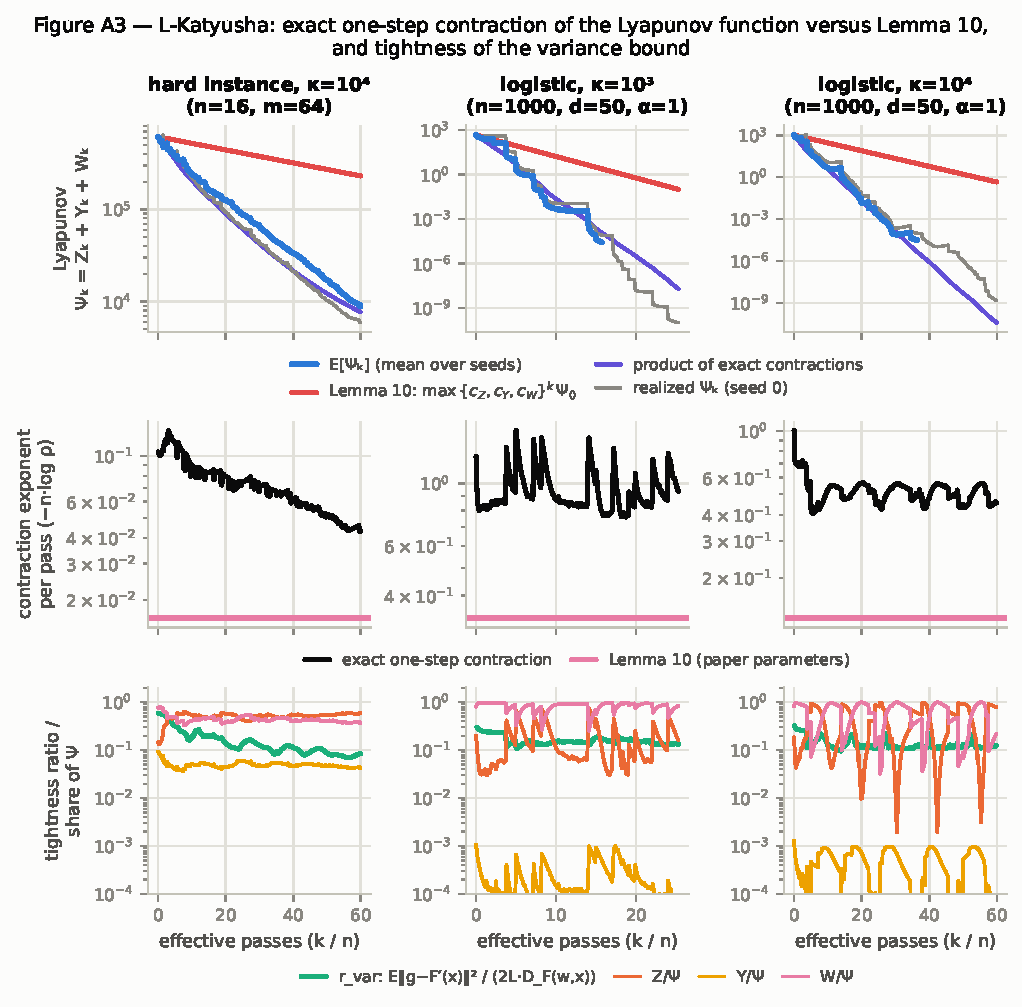
\includegraphics[width=\textwidth]{figA3_lkatyusha_lyapunov}
  \caption{\textbf{Hypothesis A3: the Lyapunov proof of L-Katyusha, measured.} L-Katyusha with the parameters of
  Theorem~11 of~\cite{kovalev2020dont} ($\theta_2=\frac12$, $\theta_1=\min\{\sqrt{2n/(3\kappa)},\frac12\}$, $p=\frac1n$) on (H)
  ($n=16$, $m=64$, $\kappa=10^4$) and on logistic regression ($n=1{,}000$, $d=50$, $\alpha=1$, $\kappa\in\{10^3,10^4\}$),
  3 seeds, records with $\Psi_t<10^{-10}$ discarded (the iteration counter is written $k$ in the figure). Top: the
  Lyapunov function $\Psi_t=Z_t+Y_t+W_t$ (mean over seeds), the contraction $\max\{c_Z,c_Y,c_W\}^t\Psi_0$ certified by
  Lemma~10 of~\cite{kovalev2020dont} (inequality~\eqref{ineq:contraction}), the product of the exact conditional
  contractions along seed $0$ and the realized $\Psi_t$ of seed $0$. Middle: exact one-step contraction exponent per pass
  along seed $0$ against the certified one. Bottom (seed $0$): tightness of the variance bound
  $\E\norm{g-\Fp(x)}^2\le2L\,D_F(w,x)$ and shares of $Z$, $Y$ and $W$ in $\Psi$.}
  \label{fig:A3}
\end{figure}

The proof thus holds along the trajectories. Its looseness ($2.8$ and $4.1$ at $\kappa=10^3$ and $10^4$ on logistic
regression, $4.7$ on (H)) is smaller than that of Proposition~\ref{prop:59} on the same logistic problems ($5.2$ and
$15.7$) and grows less between these two values of $\kappa$ ($\times1.5$ against $\times3.1$); two values of $\kappa$, in
different regimes of the certificate ($c_W$ binding at $\kappa=10^3$, where $\theta_1=\frac12$, and $c_Z$ at $10^4$), do not
determine how it scales. Both certificates have the optimal order in the worst case, by the lower bounds of
Section~\ref{sec:th-A1} for L-Katyusha and by \resref{prop:B3-lower} for SAGA, so the difference concerns these instances,
not the order of the bounds. On the two ill-conditioned problems the cancelled term exceeds the whole certified decrease
on about two thirds of the steps, as the part of prediction (P4) of Section~\ref{sec:lk-naive} on L-Katyusha anticipates.
On most of these steps, however, it has the favourable sign ($c(t)<0$ on $84\%$ and $70\%$ of them, against none of the
$5\%$ of such steps at $\kappa=10^3$): if $c(t)\le0$, then $D_F(w_t,x_t)\le F(w_t)-F(x_t)$, a difference of function values,
which a reference potential can pay. The sign-aware ratio $q_+(t)$, which counts the cancelled term only where $c(t)>0$, is
at least $1$ on $9.9\%$, $5.2\%$ and $19.3\%$ of the recorded states, that is, on $43\%$, $23\%$ and $54\%$ of the states
with $c(t)>0$: only there could the cancelled term not have been absorbed into the certified decrease, which is the
mechanism behind predictions (P2) and (P3) of Section~\ref{sec:lk-naive} for the naive scheme.

% -----------------------------------------------------------------------------------------------------
% A2. Sources: results/A2_summary.json and digest.md A2 tables (one seed; gradients to 1e-10 for the trajectories, read at
% the first record below the target, to 1e-6 for the grid, interpolated log-linearly between records by
% vrlab.algorithms.grads_to_accuracy; counts in units of n as in the titles and cells of Figure A2); counts with stored
% reference gradients: grad_evals - iters at the stop in results/A2.pkl; A3 note (Def. naive, Rem. naive-book, Props.
% naive, naive-kappa, prediction (P2)); findings.md Sec. 6; Allen-Zhu Sec. 7.1 as quoted in the A3 note and in the
% related-work section. Dimension condition (ineq:dim) for kappa = 1e4, at 1e-6 and 1e-10: right-hand sides 86.4 and
% 143.9 (144.0 in the sqrt form) with Q = 1 + (kappa - 1)/n; 108.3 and 180.6, i.e. m >= 109 and m >= 181, with
% q = 0.93823 for Q_b = 1 + 4c/mu_b = 984.47 of (H) (q + 1/q = 2 + mu_b/c, c = 245.87 from
% vrlab.problems.make_hard_instance(16, 64, 1e4)); q^(2m) = 2.9e-4 at m = 64 (q^(2m) = 1.04e-6 > 1e-6 at m = 108).
% -----------------------------------------------------------------------------------------------------
\subsection{Naive acceleration (hypothesis A2)}\label{sec:exp-A2}

What happens when Nesterov's momentum is combined with the loopless-SVRG estimator $g=\fip(x)-\fip(w)+\Fp(w)$ without the
negative momentum of Katyusha? We test L-Katyusha with $\theta_2=0$ and the same $\theta_1$, $\eta$, $p$, that is, the
scheme of \resref{def:naive} with $\eta=1/(3\theta_1)$, and the two-sequence form
$v=\theta+\beta(\theta-\theta_{\rm prev})$, $\theta^+=v-\gamma g(v)$, with the reference point reset to $v$ with
probability $\frac1n$, tuned over $\beta\in\{0.5,0.8,0.9,0.95,(\sqrt\kappa-1)/(\sqrt\kappa+1)\}$ and
$\gamma R^2\in\{\frac16,\frac1{20},\frac1{60}\}$ (best setting: fewest gradients to the relative error $10^{-6}$). The
latter is a variant of \resref*{def:naive} without the drift term of \resref{rem:naive-book}, with the reference point
reset to the query point instead of the gradient-step iterate, and with $(\beta,\gamma)$ free; \resref{prop:naive} and
\resref{prop:naive-kappa} are proved for \resref*{def:naive} only. Both schemes are compared with SAGA, L-SVRG, L-Katyusha
with the untuned parameters of its theorem, and AGD, on (H) with $m=64$, $\kappa=10^4$, and on logistic regression with
$\kappa=10^4$, $\alpha=1$ (one seed each, Figure~\ref{fig:A2}). With $m=64$, the analogue for (H) of the dimension
condition~\eqref{ineq:dim} of \resref{cor:count}, $q^{2m}\le\varepsilon$ with $q=(\sqrt{Q_b}-1)/(\sqrt{Q_b}+1)=0.938$ and
$Q_b=1+4c/\mu_b$ (Section~\ref{sec:setting}), fails at the accuracies $10^{-6}$ and $10^{-10}$ used here, which need
$m\ge109$ and $m\ge181$: the lower bound is not certified on this instance, and the certified window is explored with
$m=256$ in Section~\ref{sec:exp-A4}.

\begin{figure}[tbp]
  \renewcommand{\thefigure}{A2}% project figure name (see the header of this file)
  \centering
  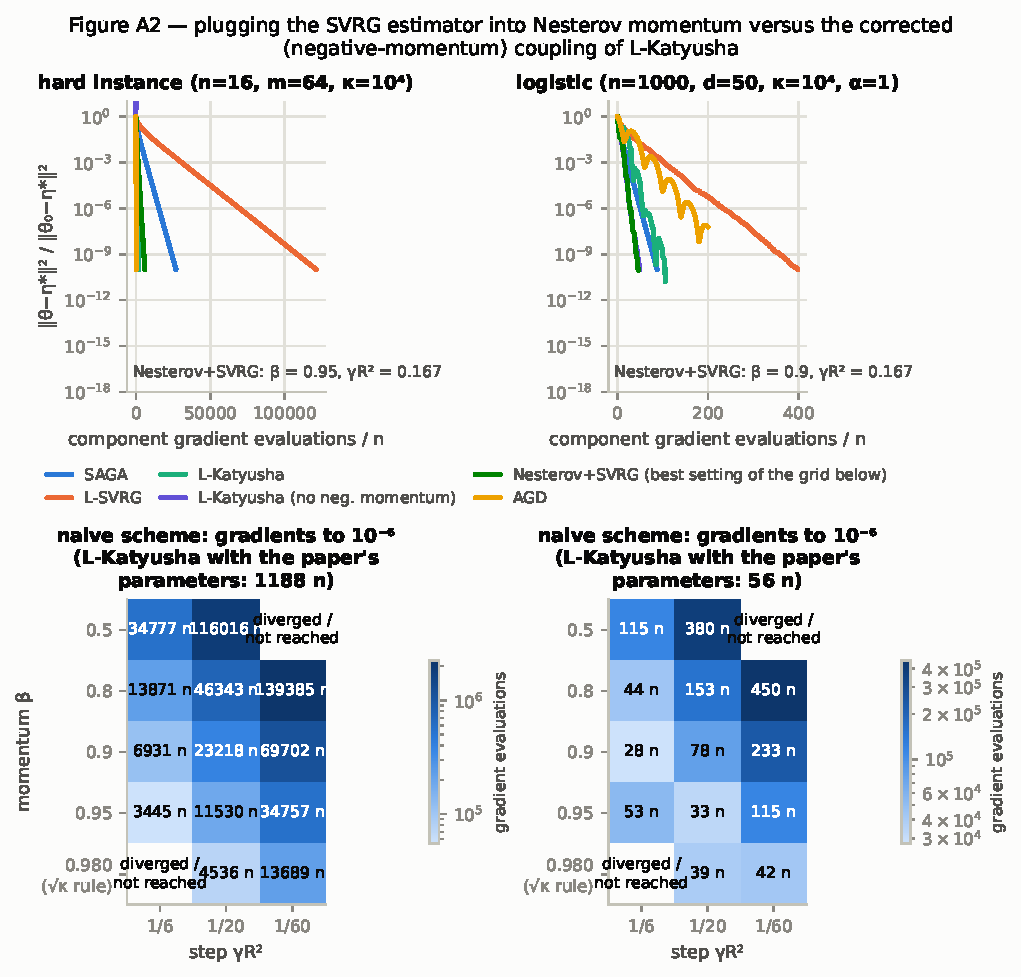
\includegraphics[width=\textwidth]{figA2_naive_acceleration}
  \caption{\textbf{Hypothesis A2: naive acceleration.} Top: relative error $\norm{\theta-\etastar}^2/\norm{\theta_0-\etastar}^2$
  (for L-Katyusha, $\theta=y_t$) against component gradient evaluations (counted as in Section~\ref{sec:exp-protocol})
  divided by $n$, for SAGA, L-SVRG, L-Katyusha (parameters of Theorem~11 of~\cite{kovalev2020dont}), L-Katyusha without
  the negative-momentum term ($\theta_2=0$), Nesterov momentum applied to the loopless-SVRG estimator (best setting of the
  grid below, given in each panel) and AGD, on (H) ($n=16$, $m=64$, $\kappa=10^4$) and on logistic regression ($n=1{,}000$, $d=50$,
  $\kappa=10^4$, $\alpha=1$); one seed, runs stopped at the first record below $10^{-10}$. Bottom: gradient evaluations needed
  by the naive scheme to reach the relative error $10^{-6}$ (interpolated log-linearly between records) for each
  $(\beta,\gamma R^2)\in\{0.5,0.8,0.9,0.95,(\sqrt\kappa-1)/(\sqrt\kappa+1)\}\times\{\frac16,\frac1{20},\frac1{60}\}$ (white cells:
  divergence or budget exhausted); the titles give the count of L-Katyusha with its untuned parameters.}
  \label{fig:A2}
\end{figure}

On (H), reaching $10^{-10}$ (counts read at the first record below the target) costs $5.3\cdot10^3$ gradients to AGD,
$3.2\cdot10^4$ to L-Katyusha, $9.6\cdot10^4$ to the best naive setting ($\beta=0.95$, $\gamma R^2=\frac16$),
$4.3\cdot10^5$ to SAGA and $1.9\cdot10^6$ to L-SVRG, while L-Katyusha with $\theta_2=0$ diverges (relative error
$8.8\cdot10^{27}$ after $3.4\cdot10^3$ gradients). With the rule $\beta=(\sqrt\kappa-1)/(\sqrt\kappa+1)=0.980$ the naive
scheme diverges at $\gamma R^2=\frac16$ and needs $4536n$ and $13\,689n$ gradients to reach $10^{-6}$ at
$\gamma R^2=\frac1{20}$ and $\frac1{60}$, against $1188n$ for L-Katyusha; the best setting of the grid needs $3445n$,
$2.9$ times more. AGD is the cheapest here because $L_F=R^2/n$ (Section~\ref{sec:exp-A4}). On logistic regression the
order of AGD, L-Katyusha and the best naive setting is reversed: reaching $10^{-10}$ costs $4.7\cdot10^4$ gradients to the
best naive setting ($\beta=0.9$, $\gamma R^2=\frac16$), $4.9\cdot10^4$ to L-Katyusha with $\theta_2=0$, $8.8\cdot10^4$ to
SAGA, $1.06\cdot10^5$ to L-Katyusha ($7.1\cdot10^4$, fewer than SAGA, with stored reference gradients) and $4.0\cdot10^5$
to L-SVRG, while AGD ($L_F/\mu=654$) is still at $6.1\cdot10^{-8}$ after 200 passes; to $10^{-6}$, the best naive setting
needs $28n$ against $56n$ for L-Katyusha, and the $\sqrt\kappa$ rule fails at $\gamma R^2=\frac16$ (final relative error
$1.26$ after 200 passes) and needs $39n$ and $42n$ at the smaller steps.

On (H) the negative momentum is what keeps the coupling stable: removing it produces the divergence anticipated by
prediction (P2) of Section~\ref{sec:lk-naive} for $\kappa\gg n$, and the momentum scheme must be detuned, which costs it
the advantage over L-Katyusha. \resref{prop:naive} and \resref{prop:naive-kappa} describe the same obstruction in the
proof, for the scheme of \resref{def:naive}: without the anchor the one-step inequality keeps the uncontrolled term
$\frac\nu{\theta_1}D_F(w_t,x_t)$, and closing it with smoothness and strong convexity costs a factor $\kappa$. On a benign
logistic problem, whose effective constants are much better than the worst-case ones ($\muEff\approx5\mu$ near $\etastar$
and $\LEff\approx R^2/9$ along SAGA, Section~\ref{sec:exp-B2}), the anchor-free schemes converge and are about twice as
fast as L-Katyusha with worst-case parameters ($\theta_1=\sqrt{2n/(3\kappa)}=0.26$), in line with the report
of~\cite[Section~7.1]{allenzhu2018katyusha} that the scheme without negative momentum is sometimes faster after careful
tuning but does not accelerate on some tasks. These observations come from two instances, one seed and a grid that favours
the naive scheme (fifteen settings against an untuned L-Katyusha); they do not show that it cannot accelerate, a question
that no lower bound known to us settles, as noted in \resref{rem:naive-honest}.

% -----------------------------------------------------------------------------------------------------
% A4. Sources (final sweeps): results/A4_summary.json ((H) and (R): per-kappa geometric means and min/max over the 3
% seeds, slopes over kappa >= 10n with 95% t-intervals, K = 6; the only instances with L-SVRG and the naive schemes),
% results/A4b_summary.json ((S) and (A): slopes against the nominal kappa and against kappa_eff, over x >= 10n and over
% the window 10n <= kappa <= kappa_max, counts, kappa_eff, kappa_max), results/A4.pkl (status of the 294 runs; key
% "grid": settings selected for the naive scheme), results/A4b.pkl (seed spreads), findings.md Sec. 7. Ratios of counts,
% local slopes, seed spreads and kappa_eff/kappa are computed from these files (per-kappa geometric means over the
% seeds), and so are the fits over 10n <= kappa <= 3e4 on (H) (vrlab.analysis.loglog_slope: SAGA 1.008, L-Katyusha
% 0.510). Dimension condition on (H): q^(2m), q = (sqrt(Q)-1)/(sqrt(Q)+1), Q = 1 + 4c/mu_b, computed from the
% constants of make_hard_instance: 1.2e-10 at kappa = 3e4, 1.2e-5 at kappa = 1e5, equal to eps = 1e-8 at kappa = 4.4e4
% (findings.md Sec. 7(a); comment of experiments/exp_A4_hard_instance.py). Results referred to with \resref: A1 note,
% Props. constants, anyseq, sagamean, A4 (eq:window, eq:sagawindow, eq:lkwindow), Cor. saga, Lemma overlap, Rem. plot
% (and Sec. lb:predictions); B3 note, Prop. B3-lower; A3 note, Def. naive, Prop. naive-kappa. Factors of the two sides
% of eq:sagawindow and eq:lkwindow on (S) (7.76--7.84 and 88.6--114.9, with rho and C0 replaced by their bounds 1/105 and
% 1 + 5Q/8): Section th-A1, after Prop. A4 (6.5 for SAGA with the exact rho, Rem. plot).
% -----------------------------------------------------------------------------------------------------
\subsection{Complexity exponents on hard instances (hypothesis A4)}\label{sec:exp-A4}

\paragraph{Question and setting.}
Hypothesis A4 predicts that, for $\kappa\gg n$, the number $T$ of component gradients needed to reach
$\norm{\theta-\etastar}^2\le\varepsilon\norm{\theta_0-\etastar}^2$ grows like $\kappa$ for SAGA and like $\kappa^{1/2}$ for
L-Katyusha. On (S), \resref{prop:A4} proves $T_{\rm SAGA}=\Theta(\kappa\log\frac1\varepsilon)$ and
$T_{\rm LK}=\Theta(\sqrt{n\kappa}\log\frac1\varepsilon)$ inside the window $4n+1\le\kappa\le\kappa_{\max}(m,\varepsilon)$
of~\eqref{eq:window}, up to the constants of~\eqref{eq:sagawindow}--\eqref{eq:lkwindow} and the factor
$\log(1+\frac58Q)$ of~\eqref{eq:lkwindow}; its part (ii) gives GD and AGD the same two exponents, $L_F/\mu$ being of the
order of $Q=1+(\kappa-1)/n$ by \resref{prop:constants}. Beyond $\kappa_{\max}$ the exhaustion of the chain sets in (part
(iii) of \resref*{prop:A4}), and the counts should be read against $\kappa_{\rm eff}$, as \resref{rem:plot} explains. For $n=16$,
$m=256$ and $\varepsilon=10^{-8}$, $\kappa_{\max}\approx4.9\cdot10^4$ on (S) (the dimension term of~\eqref{eq:window}; the
slow-mode term is $1.1\cdot10^5$); on (A), a single chain of length $m=2048$, the dimension condition holds in its
sufficient form up to $(4m/\log\frac1\varepsilon)^2\approx2.0\cdot10^5$, beyond the sweep. The bounds of
Appendix~\ref{sec:lower_bound} are proved for (S), not for (H); the analogue of their dimension condition,
$q^{2m}\le\varepsilon$ with $q=(\sqrt{Q_b}-1)/(\sqrt{Q_b}+1)$ for the per-block parameter $Q_b=1+4c/\mu_b$ of (H)
(Section~\ref{sec:setting}), holds up to $\kappa\approx4.4\cdot10^4$ ($q^{2m}=1.2\cdot10^{-10}$ at $\kappa=3\cdot10^4$) and
fails at the last point of (H), $\kappa=10^5$ ($q^{2m}=1.2\cdot10^{-5}>\varepsilon$), which thus lies outside the regime in
which a span lower bound would certify the exponent $\frac12$. The counts follow the conventions of
Section~\ref{sec:exp-protocol}: for L-Katyusha the error is measured on the gradient sequence $y_t$ and $3$ gradients
are charged per iteration on average, whereas $T_{\rm LK}$ in \resref*{prop:A4} refers to the mirror sequence $z_t$ with
stored reference gradients, $2$ per iteration; the exponents are unaffected, but the measured counts of L-Katyusha are
about $\frac32$ times those of that convention, and ratios such as $T_{\rm SAGA}/T_{\rm LK}$ below are smaller by the same
factor.

On (H) and (R) the sweeps also include L-SVRG, L-Katyusha without negative momentum, and the naive scheme of
Section~\ref{sec:exp-A2}, re-tuned at every pair (instance, $\kappa$) over $\beta\in\{0.8,0.95,(\sqrt\kappa-1)/(\sqrt\kappa+1)\}$
and $\gamma R^2\in\{\frac16,\frac1{20}\}$: on (H) on seed~$0$, the choice being reused for the other seeds, and on (R),
where each seed draws a new instance, separately on each seed. Each grid run is capped at 45~s of CPU time; as the grid
runs have the same cost per iteration, a run cut by this cap had already used more gradients than the selected one
needed in total. Every run reached the target except the 30 runs of L-Katyusha without negative momentum at
$\kappa\ge10^3$, which diverge (Figures~\ref{fig:A4} and~\ref{fig:A4b}).

\begin{figure}[tbp]
  \renewcommand{\thefigure}{A4}% project figure name (see the header of this file)
  \centering
  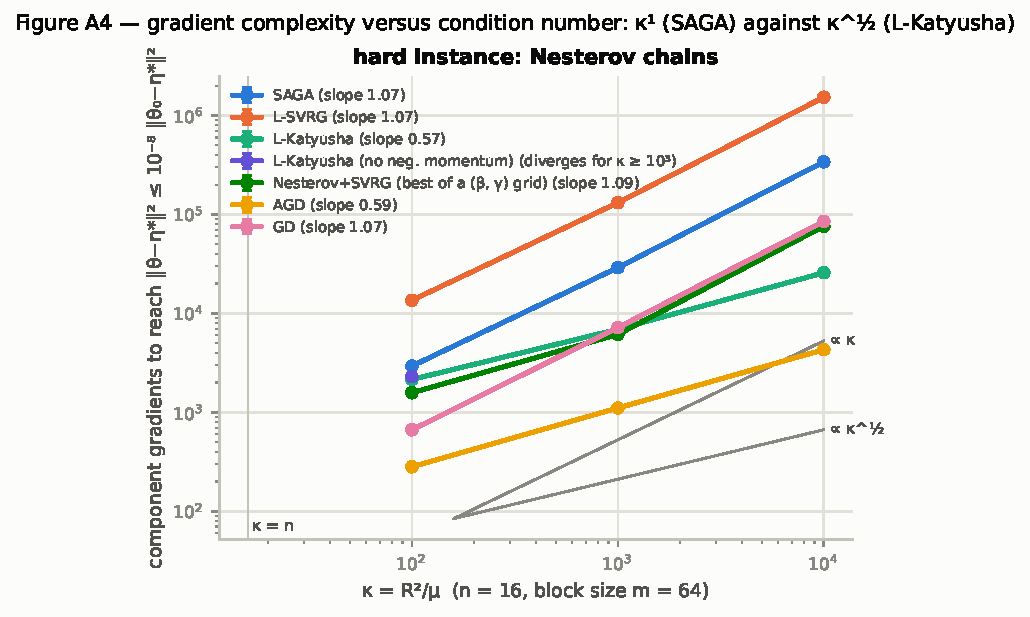
\includegraphics[width=\textwidth]{figA4_hard_instance_exponents}
  \caption{\textbf{Hypothesis A4: gradient complexity against $\kappa$.} Component gradients (counted as in
  Section~\ref{sec:exp-protocol}) needed to reach $\norm{\theta-\etastar}^2\le10^{-8}\norm{\theta_0-\etastar}^2$ (for
  L-Katyusha, $\theta=y_t$) for $\kappa\in\{10^2,3\cdot10^2,\dots,10^5\}$ ($n=16$) on (H) (block-separable Nesterov chains
  of length $m=256$, left) and on block quadratics with random spectra (R) ($m=256$, right); geometric mean over 3 seeds,
  error bars: min--max. SAGA uses $\gamma=1/(4R^2)$, L-SVRG $\gamma=1/(6R^2)$, L-Katyusha the parameters of Theorem~11
  of~\cite{kovalev2020dont}, L-Katyusha without negative momentum $\theta_2=0$ with the same $\theta_1$, $\eta$, $p$ (it
  converges only for $\kappa\in\{10^2,3\cdot10^2\}$ and diverges for every $\kappa\ge10^3$, hence no slope), the naive
  Nesterov+SVRG scheme the best of six settings
  $(\beta,\gamma R^2)\in\{0.8,0.95,(\sqrt\kappa-1)/(\sqrt\kappa+1)\}\times\{\frac16,\frac1{20}\}$, selected at each $\kappa$ on
  seed $0$ for (H) and on each seed for (R), whose instance changes with the seed, AGD and GD the step $1/L_F$. Legend:
  slope $b\pm h$, the least-squares slope of $\log(\text{gradients})$ against $\log\kappa$ fitted to the per-$\kappa$
  geometric means over the seeds, for $\kappa\ge10n$ ($K=6$), and $h$ the half-width of its $95\%$ Student interval with
  $K-2$ degrees of freedom, which measures the departure from a single power law, not sampling noise (function
  \texttt{loglog\_slope} of \texttt{vrlab/analysis.py}). Grey lines: reference slopes $1$ and $\frac12$; vertical line:
  $\kappa=n$. The only missing points are those of the divergent runs.}
  \label{fig:A4}
\end{figure}

\begin{figure}[tbp]
  \renewcommand{\thefigure}{A4b}% project figure name (see the header of this file)
  \centering
  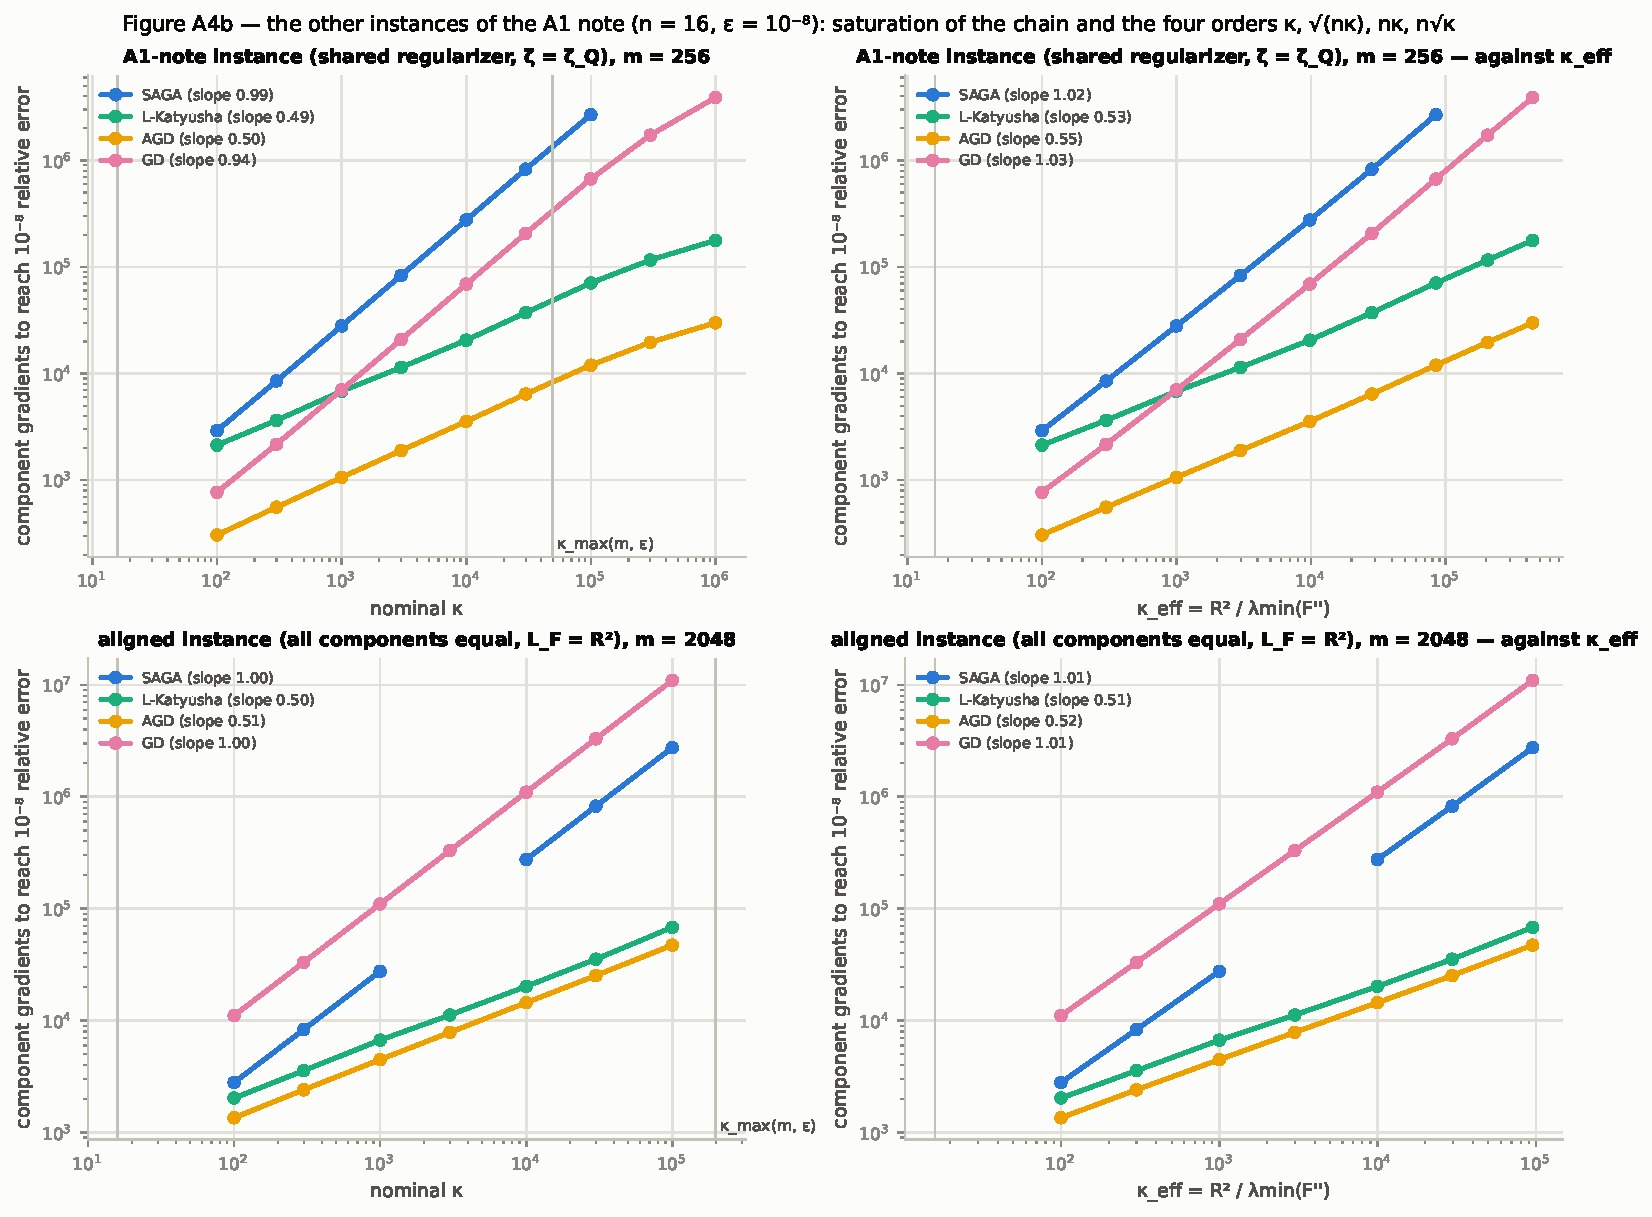
\includegraphics[width=\textwidth]{figA4b_instances}
  \caption{\textbf{Hypothesis A4 on the instances of Appendix~\ref{sec:lower_bound}.} Component gradients needed to reach
  $\norm{\theta-\etastar}^2\le10^{-8}\norm{\theta_0-\etastar}^2$ ($n=16$; geometric mean over 2 seeds; for L-Katyusha,
  $\theta=y_t$) for SAGA ($\gamma=1/(4R^2)$), L-Katyusha (parameters of Theorem~11 of~\cite{kovalev2020dont}), AGD and GD
  (step $1/L_F$), all tuned with the exact constants of the instance; L-Katyusha and AGD receive $\lmin(F'')$, not $\mu$,
  as their strong-convexity constant, so that on (S) their parameters depend on $\kappa_{\rm eff}$, not on the nominal
  $\kappa$. Top: the
  instance (S) of~\eqref{eq:instance} (shared regularizer, $\zeta=\zeta_Q$, $m=256$),
  $\kappa\in\{10^2,3\cdot10^2,\dots,10^6\}$. Bottom: the aligned instance (A) (all
  components equal to one chain of length $m=2048$, $L_F=R^2$), $\kappa\in\{10^2,3\cdot10^2,\dots,10^5\}$, on which GD and
  AGD pay the factors $n$ and $\sqrt n$ that they do not pay on (S). Left: against the nominal $\kappa$; right: against
  $\kappa_{\rm eff}=R^2/\lmin(F'')$. In the left panels the vertical line on the right marks $\kappa_{\max}(m,\varepsilon)$
  of~\eqref{eq:window} ($\approx4.9\cdot10^4$, top) and its single-chain analogue
  $(4m/\log\frac1\varepsilon)^2\approx2.0\cdot10^5$ (bottom, beyond the sweep), beyond which the chain is exhausted and the
  lower-bound argument for the exponent $\frac12$ no longer applies; in every panel the vertical line on the left marks
  $\kappa=n$. Legend: slope $b\pm h$, the least-squares slope of $\log(\text{gradients})$ against the logarithm of the
  abscissa, fitted to the per-$\kappa$ geometric means over the seeds for abscissae at least $10n$ ($K=8$ at the top, $6$
  at the bottom), and $h$ the half-width of its $95\%$ Student interval with $K-2$ degrees of freedom (function
  \texttt{loglog\_slope} of \texttt{vrlab/analysis.py}); the slopes restricted to the window
  $10n\le\kappa\le\kappa_{\max}(m,\varepsilon)$ are given in Section~\ref{sec:exp-A4}. All runs reached the target.}
  \label{fig:A4b}
\end{figure}

\paragraph{Exponents.}
The slopes $b\pm h$ of Section~\ref{sec:exp-protocol}, against $x=\kappa$ (nominal) or $x=\kappa_{\rm eff}$, are, over
$x\ge10n$ unless the window $10n\le\kappa\le\kappa_{\max}$ is indicated (the five values of the nominal $\kappa$ of (S)
from $3\cdot10^2$ to $3\cdot10^4$; L-SVRG and the naive scheme were run on (H) and (R) only):
\begin{center}
\footnotesize
\setlength{\tabcolsep}{3.5pt}
\begin{tabular}{@{}lcllllll@{}}
\toprule
instance, $x$ & $K$ & SAGA & L-SVRG & L-Katyusha & naive scheme & AGD & GD \\
\midrule
(H), $\kappa$ & 6 & $1.022\pm0.025$ & $1.021\pm0.026$ & $0.525\pm0.027$ & $0.806\pm0.188$ & $0.550\pm0.010$ & $1.026\pm0.021$ \\
(R), $\kappa$ & 6 & $1.0025\pm0.0001$ & $1.002\pm0.001$ & $0.500\pm0.005$ & $0.814\pm0.166$ & $0.526\pm0.013$ & $1.007\pm0.004$ \\
(S), $\kappa$ & 8 & $0.945\pm0.048$ & -- & $0.490\pm0.022$ & -- & $0.501\pm0.027$ & $0.944\pm0.047$ \\
(S), $\kappa$, window & 5 & $0.994\pm0.004$ & -- & $0.500\pm0.020$ & -- & $0.530\pm0.005$ & $0.990\pm0.008$ \\
(S), $\kappa_{\rm eff}$ & 8 & $1.031\pm0.017$ & -- & $0.533\pm0.019$ & -- & $0.547\pm0.007$ & $1.029\pm0.018$ \\
(S), $\kappa_{\rm eff}$, window & 5 & $1.005\pm0.015$ & -- & $0.506\pm0.025$ & -- & $0.536\pm0.009$ & $1.002\pm0.019$ \\
(A), $\kappa$ & 6 & $0.999\pm0.001$ & -- & $0.502\pm0.015$ & -- & $0.511\pm0.003$ & $0.9991\pm0.0004$ \\
(A), $\kappa_{\rm eff}$ & 6 & $1.006\pm0.008$ & -- & $0.506\pm0.018$ & -- & $0.515\pm0.006$ & $1.006\pm0.007$ \\
\bottomrule
\end{tabular}
\end{center}
On (H) and (R) the slopes are close to $1$ for SAGA, L-SVRG and GD and to $\frac12$ for L-Katyusha and AGD; the largest
deviations are those of AGD and of (H), whose local slopes rise over the last two intervals of $\kappa$ (SAGA $1.04$ and
$1.08$, L-Katyusha $0.56$ and $0.58$) and whose last point fails the analogue of the dimension condition: without this
point, the fits on (H) give $1.008$ for SAGA and $0.510$ for L-Katyusha. On (S), against the nominal $\kappa$, SAGA and
GD have the slopes $0.95$ and $0.94$, with intervals $[0.90,0.99]$ that exclude $1$: the points beyond $\kappa_{\max}$ bend
both curves (local slopes $0.98$, $0.86$ and $0.67$ between $3\cdot10^4$, $10^5$, $3\cdot10^5$ and $10^6$), whereas inside
the window their slopes are $0.994\,[0.990,0.998]$ and $0.990\,[0.982,0.998]$. On (A), where every $\kappa$ lies in the
window, they are $0.999$, against $0.50$ and $0.51$ for L-Katyusha and AGD. Several intervals exclude the predicted
exponent, by at most $0.01$ for SAGA, L-SVRG, L-Katyusha and GD on (H), on (R) and inside the windows, and by up to
$0.04$ for AGD: they measure the lack of fit of a single power law, and \resref{prop:A4} predicts the exponents only as
orders of growth, up to constant and logarithmic factors.

The naive scheme has the fitted slopes $0.81$ on both (H) and (R), with wide intervals, $[0.62,0.99]$ and $[0.65,0.98]$,
which nevertheless exclude $\frac12$; it does not follow a power law. Its best setting is the same on both instances:
$\beta=0.95$ with $\gamma R^2=\frac1{20}$ at $\kappa=10^2$, $\beta=0.95$ with $\gamma R^2=\frac16$ at
$\kappa\in\{3\cdot10^2,10^3,10^4\}$, and $\beta=(\sqrt\kappa-1)/(\sqrt\kappa+1)$ with $\gamma R^2=\frac16$ at $3\cdot10^3$ and
with $\gamma R^2=\frac1{20}$ at $\kappa\in\{3\cdot10^4,10^5\}$ (on (R) one seed selects $\beta=(\sqrt\kappa-1)/(\sqrt\kappa+1)$,
with $\gamma R^2=\frac16$, already at $\kappa=3\cdot10^2$). Its local slopes between consecutive values of $\kappa$ are
$0.82$, $0.28$, $0.73$, $1.30$, $0.79$, $0.58$
on (H) and $0.65$, $0.45$, $0.75$, $1.29$, $0.75$, $0.50$ on (R): close to $\frac12$ from $3\cdot10^2$ to $3\cdot10^3$ ($0.50$
and $0.59$; $\beta=0.95$ is the momentum $(\sqrt\kappa-1)/(\sqrt\kappa+1)$ of $\kappa\approx1.5\cdot10^3$), a jump of slope
about $1.3$ between $3\cdot10^3$ and $10^4$, then $0.5$ to $0.8$. L-Katyusha without negative momentum converges at
$\kappa=10^2$ and $3\cdot10^2$ and diverges for every $\kappa\ge10^3$ on both instances.

\paragraph{Constants, $L_F$ and finite dimension.}
On the block-separable instances the full-gradient methods share the exponents of the variance-reduced ones with
smaller constants. At $\kappa=10^5$, reaching the target costs, on (H) and (R), $1.47\cdot10^7$ and $1.49\cdot10^7$
gradients to L-SVRG, $3.27\cdot10^6$ and $3.31\cdot10^6$ to SAGA, $8.2\cdot10^5$ and $8.3\cdot10^5$ to GD, $3.1\cdot10^5$ to the
naive scheme, $7.85\cdot10^4$ to L-Katyusha and $1.3\cdot10^4$ to AGD. L-SVRG costs $4.5$ times SAGA at every
$\kappa\ge10^3$ ($4.5$--$4.6$ overall): its step $1/(6R^2)$ instead of $1/(4R^2)$ and the $3$ gradients per iteration
charged to it give $1.5\times3$ (the factor would be $3$ with stored reference gradients). The ratio
$T_{\rm GD}/T_{\rm SAGA}$ is $0.25$ on (H), (R) and (S) for every $\kappa\ge10^3$ and $4.0$ on (A) for every
$\kappa\ge10^4$; both values equal $nL_F/(4R^2)$ up to rounding, the ratio expected if the error of SAGA decays like that of
its mean iterate, which follows gradient descent with step $1/(4R^2)$ and one gradient per iteration by
\resref{prop:sagamean}, since $L_F\approx R^2/n$ on the block-separable instances and $L_F=R^2$ on (A). The counts of SAGA and of L-Katyusha agree
within $6\%$ between (S) and (A) at every common nominal $\kappa$, whereas GD costs $14$ to $16$ times more and AGD $3.9$ to
$4.4$ times more on (A): about $n$ and $\sqrt n$, the factors by which $nL_F/\mu$ and $n\sqrt{L_F/\mu}$ grow when $L_F$ goes
from about $R^2/n$ to $R^2$. The ratio $T_{\rm SAGA}/T_{\rm LK}$ grows like $\sqrt{\kappa/n}$, with a constant between $0.52$
and $0.54$ over the whole sweep on (H) and (R) ($41.7$ and $42.1$ at $\kappa=10^5$, where $\sqrt{\kappa/n}=79$), between
$0.51$ and $0.55$ on (A), and of $0.54$ and $0.48$ at $\kappa=10^4$ and $10^5$ on (S) ($13$ and $38$); with the counting
convention of \resref{prop:A4}, which stores the reference gradients, these constants would be about $\frac32$ times
larger. On (S), $\kappa_{\rm eff}/\kappa$ is $0.98$ at the nominal $\kappa=10^4$, $0.85$ at $10^5$ and $0.44$ at $10^6$; the
slopes of SAGA and GD drop from $0.99$ inside the window to $0.95$ and $0.94$ over $\kappa\ge10n$ against the nominal
$\kappa$, and are both $1.03$ against $\kappa_{\rm eff}$: plotting against $\kappa_{\rm eff}$ largely removes the bend, as
part (iii) of \resref*{prop:A4} and \resref{rem:plot} anticipate, with a slight overshoot (local slopes against
$\kappa_{\rm eff}$ up to $1.07$ between $3\cdot10^4$ and $3\cdot10^5$). L-Katyusha and AGD, whose parameters depend on
$\lmin(F'')$, i.e.\ on $\kappa_{\rm eff}$, rather than on $\mu$, bend less ($0.50$ to $0.49$ and $0.53$ to $0.50$), and
their slopes against $\kappa_{\rm eff}$, $0.53$ and $0.55$, are slightly above $\frac12$. The theory does not fix these
values: inside the window its bounds leave constant and logarithmic factors, such as the $\log(1+\frac58Q)$
of~\eqref{eq:lkwindow}, and beyond $\kappa_{\max}$ the lower bound behind the exponent $\frac12$ no longer applies, while
the upper bounds involve $\lmin(F'')$ rather than $\mu$ because of this tuning (for L-Katyusha, part (iii) of
\resref*{prop:A4}, with $\kappa_{\rm eff}$ in place of $\kappa$).

\paragraph{Interpretation.}
The exponents predicted by hypothesis A4 are observed on the four instances with 2 or 3 seeds, up to the constant and
logarithmic factors of \resref{prop:A4}: over $\kappa\ge10n$ and against the nominal $\kappa$, the slopes are $0.95$--$1.02$
for SAGA ($0.95$ on (S), whose chain is exhausted beyond $\kappa_{\max}$; $0.99$ inside its window and $1.03$ against
$\kappa_{\rm eff}$), $1.00$--$1.02$ for L-SVRG (on (H) and (R), the two instances where it was run) and $0.49$--$0.52$ for
L-Katyusha. As orders of growth, the exponent $1$ of SAGA is a theorem for constant steps, by \resref{prop:B3-lower},
and, on (S) and (A), inside their windows and for the step $1/(4R^2)$ of the experiments, by \resref{cor:saga} with
\resref{lem:overlap}; on (S) the exponent $\frac12$ of L-Katyusha is optimal inside the window, by \resref{prop:anyseq}
with part (ii) of \resref*{prop:A4}. The measured slopes agree with these orders, which do not by themselves fix the
value of a slope fitted over a finite window: the two sides of~\eqref{eq:sagawindow} and of~\eqref{eq:lkwindow}, with
$\rho$ and $C_0$ replaced by their bounds, differ there by factors of about $8$ and $10^2$ (Section~\ref{sec:th-A1} and
\resref*{rem:plot}).
The expectation of the proposal that AGD costs $n\sqrt\kappa$ and GD $n\kappa$ holds only when $L_F\approx R^2$, as on
(A): on block-separable instances, the worst case for incremental methods, the full-gradient methods do at least as well
as their variance-reduced counterparts, and what variance reduction buys is the uniform guarantee over all instances with
given $(n,R^2,\mu)$ (Section~\ref{sec:lb:predictions}). The re-tuned naive scheme, a variant of the scheme
of \resref{def:naive} (Section~\ref{sec:exp-A2}), has fitted slopes between the two exponents on this grid. This is
consistent with, but not predicted by, the obstruction that \resref{prop:naive-kappa} proves for the scheme
of \resref*{def:naive} itself, a limit of the proof, and with the absence of an acceleration guarantee for such schemes
with one sample per iteration~\cite{nitanda2014stochastic}; it does not show that no tuning can accelerate the scheme.



\section{Discussion}\label{sec:discussion}
% =====================================================================================================
% Discussion (the \section and the label sec:discussion are in main.tex; this file has no \section).
% Every number is quoted from Section sec:experiments (same sources: results/digest.md, results/*_summary.json,
% results/findings.md). The A4 and A4b sweeps are final (results/A4_summary.json, results/A4b_summary.json,
% findings.md Sec. 7): slopes are least-squares fits of the per-kappa geometric means over kappa >= 10n, with 95%
% t-intervals with K-2 degrees of freedom. The hypotheses are stated in the introduction (paragraph Hypotheses).
% Citations: claims as in related.tex and bibliography/literature_review.md (Sections 6, 8, 9); for A1, the
% assessment of hypothesis (A1) in Appendix A1 (theory/A1_lower_bound.tex, Sec. lb:statements, items (i)-(iv)).
% A3: A3 note, Outcome and the reading of q and q_+ in Sec. lk-instrument (A3_summary.json: q >= 1 on 63%, 5%, 65% of
% the steps; q_plus_frac_ge_1 0.0986, 0.0519, 0.1929 for (H), logistic kappa = 1e3, 1e4). Growth from kappa = 1e3 to
% 1e4 (alpha = 1): 4.117/2.775 = 1.48 (A3_summary.json, speedup_exact_over_lemma) against 15.734/5.155 = 3.05
% (B3_summary.json, attribution, speedup).
% Results of the appendices are referred to with \resref{label} (report/restate_defs.tex).
% B1: B1 note, Step 2 of the proof and outcome paragraph (E V_t^P >= 3 gamma^2 (1-1/n)^t M_0); B1.pkl (memory
% coefficient about 1-0.65/n, r_sq 0.51-0.53, r_var about 1). A2: A2_summary.json and A2.pkl (with storage of the
% reference gradients, i.e. grad_evals - iters: L-Katyusha 71400 against SAGA 87800 on logistic regression).
% A4: naive/L-Katyusha at kappa = 1e4 (A4_summary.json): 3.01 on (H), 2.99 on (R).
% =====================================================================================================

\paragraph{B3: where the proof of Proposition~\ref{prop:59} loses.}
The diagnosis was carried out and locates the loss, which depends on the regime. On $\ell_2$-regularized logistic
regression ($n=1000$, $d=50$, 5 seeds) the exact one-step contraction exponent of SAGA, averaged over passes 2--20,
exceeds the certified one by a factor $3.2$--$3.7$ for $\kappa\le10^2$ and $19$--$220$ at $\kappa=10^5$. For $\kappa\gg
n$ the steps that cost are those that replace a quantity depending on the iterate by a global constant: for
$\kappa\ge10^4$, cocoercivity with $R^2=\max_iL_i$ (I2) and strong convexity with $\mu=\lambda$ (I4) carry
$0.77$--$0.96$ of the logarithmic gap in proof order. For $\kappa\le10^2$, where the memory term is active, the gap is
carried in proof order by the square-norm step I1 ($0.39$--$0.44$) and by I2 ($0.32$--$0.37$), and in order~A by I5
and I1. The variance step (I3) is nearly tight ($r_{\rm var}\ge0.958$; at most $0.6\%$ of the gap in proof order,
$6.3\%$ in order~A) and the minimum of the two rates (I5) matters only when $\kappa\lesssim n$. The additive shares hide
a multiplicative structure: the $\kappa$-dependent part of the gap is the factor $\muEff/\mu$ of I4, whereas, by
\resref{prop:B3-representation}, I1 and I2 together can contribute at most $\frac83$ at the fixed step (measured
$2.45$--$2.62$), and the product of the two reproduces $91$--$96\%$ of the speed-ups for $\kappa\ge10^4$. By
\resref{prop:B3-optimum} and~\resref*{rem:B3-conclusion}, optimizing $(\gamma,\Delta)$ within the proof gains $17\%$
at $\kappa=10^3$ (at most $\frac43$ whenever $\kappa\ge\frac{9n}{16}$), but up to a factor $2.4$--$2.9$ for
$\kappa\le10^2$, comparable to the whole gap there; and, by \resref{prop:B3-lower}, no analysis of SAGA with a constant
step can remove the exponent $1$ of $\kappa$. The theorem has the right order in the worst case; on these instances it
is pessimistic by a factor $3.2$--$3.7$ already for $\kappa\le10^2$, and its pessimism grows with $\kappa$ because the
curvature met along the trajectory exceeds $\mu$ by a factor that grows with $\kappa$ (up to $81$ here).

\paragraph{B2: trajectory-dependent constants.}
Confirmed in its main claim, with one refuted prediction. By \resref{cor:B2-local}, near $\etastar$, $\muEff/\mu$ is
bounded below by about $\lmin(F''(\etastar))/\mu$ (up to $70$ in our problems), a value that SAGA reaches when its error
aligns with the flattest direction, and $R^2$ overestimates $\LEff$ by a factor $2.6$ to $86$; the a-posteriori bound
with $\muEff$ and $\LEff$ (\resref*{prop:B3-traj}) recovers $0.59$--$0.96$ of the logarithmic gap for $\kappa\ge10^4$,
and nothing for $\kappa\le10^2$, where the bound is saturated by the memory term. Our prediction that the error of SAGA
stays spread over many directions holds only for $\kappa\lesssim n$, and not in every run with $\kappa\approx n$: at
$\kappa=10^4=10n$ and for $\alpha\in\{0,1\}$ (one run each) SAGA keeps and sharpens, as gradient descent does, the
alignment of the error with the flattest direction of $F''(\etastar)$, on which the initial error already carries
$89$--$98\%$ of its squared norm, a behaviour that \resref{rem:B2-P2-outcome} explains only heuristically; for
$\alpha=2$, whose spectrum is nearly degenerate at the bottom, neither method aligns within our runs. The effective constants are
a-posteriori quantities: they explain an observed trajectory, they do not certify one in advance, and, by
\resref{rem:B2-what-explains}, at a fixed step the gain from $\LEff$ is capped at $\frac83$.

\paragraph{B1: preconditioned SAGA.}
Nuanced. For logistic regression no fixed metric improves the global condition number: $\kappaP\ge\kappa$ by
\resref{prop:B1-nofreelunch}, so that \resref{cor:B1-rate} never favours preconditioning. Yet at $\kappa=10^3$ the
statistical and Hessian metrics raise the observed exponent per pass (in component gradients; a dense metric costs
$O(d^2)$ instead of $O(d)$ per iteration, and $P=F''(\etastar)$ requires $\etastar$, an oracle benchmark) from $1.00$
to $1.11$ ($\alpha=1$) and from $0.61$ to $1.24$--$1.26$ ($\alpha=2$). The gain is local: the trajectory bound of
\resref{cor:B1-kappa-traj}, which pays the smallest per-sample curvature, does not explain it, whereas with the local
constant at the optimum, a heuristic substitution that \resref{lem:B1-asymptotic} supports only as
$\theta\to\etastar$, the bound reproduces the observed ordering but saturates at the memory term, $\frac13$ per pass,
$3.3$--$3.8$ times below the observed exponents. Along the trajectories, the exact memory coefficient accounts for a
factor of about $2$ of this gap (about
$1-\frac{0.65}n$ instead of $1-\frac1{3n}$), and the parameter part, which contracts faster but is charged at the memory
rate by I5, for most of the rest; but no bound on $\E V_t^P$ can gain more than a factor $3$ over $\frac13$, since the
memory slots that are never refreshed keep $\E V_t^P$ from decreasing faster than $(1-\frac1n)^n\approx e^{-1}$ per
pass: a factor $1.1$--$1.26$ separates the typical trajectories, whose slopes are measured, from the expectation that
the bound controls. The metric shifts the slack of the proof from cocoercivity to strong convexity, as predicted, and
the Jacobi metric does not help when the features are rotated.

\paragraph{A1: lower bounds.}
This hypothesis is theoretical; Appendix~\ref{sec:lower_bound} (Section~\ref{sec:th-A1}) assesses it against the known
bounds, restated with their exact hypotheses. The first clause holds on instances whose dimension is of the order of
the number of queries certified: span-based methods sampling i.i.d.\ from a fixed distribution need
$\Omega((n+\sqrt{n\kappa})\log\frac1\varepsilon)$, by \resref{thm:LZ} when $\kappa\ge n$ and, on the instance (S), for
every $\kappa>1$ by \resref{cor:count}. The second clause holds only in a restricted sense: for oblivious methods (up
to logarithmic factors) and for loopless methods with a full-gradient coin, full-gradient steps can divide the $n\log\frac1\varepsilon$ term by at most $1+(\log(n/\kappa))_+$, a gain only
when $\kappa\ll n$, and leave the $\sqrt{n\kappa}\log\frac1\varepsilon$ term untouched, by part~(c) of
\resref{thm:HLOY} and by \resref{thm:HXZ}. Deterministic methods, cyclic ones included, face instead
$\Omega(n\sqrt\kappa\log\frac1\varepsilon)$ for small enough $\varepsilon$ when $\kappa>73$, by \resref{thm:WS}. Two
questions remain open: for randomized methods with fully adaptive queries only an additive $n$ is proved (randomized
part of \resref*{thm:WS}), and whether randomly reshuffled span-based methods, or deterministic ones when $\kappa\le73$,
can beat $n\log\frac1\varepsilon$ is not settled. Our experiments use the lower bound only through its instance: the
exponent $\frac12$ is certified there inside the window of $\kappa$ of \resref{prop:A4}, which the dimension limits
($\kappa_{\max}\approx4.9\cdot10^4$ for $m=256$ and $\varepsilon=10^{-8}$), and the regime $\kappa\ll n$ of the second
clause was not explored numerically.

\paragraph{A3: corrected acceleration.}
Confirmed. The one-step contraction of the Lyapunov proof of L-Katyusha, \resref{thm:lk}, holds at every recorded
state and is pessimistic in exponent by a factor $2.8$--$4.7$ on our three problems ($3.7$--$9.3$ for its closed-form
rate). On the two logistic problems this is less than for Proposition~\ref{prop:59} ($2.8$ and $4.1$ against $5.2$ and
$15.7$) and grows less from $\kappa=10^3$ to $10^4$ ($\times1.5$ against $\times3.1$); two values of $\kappa$, in
different regimes of the certificate, do not show how it scales. Its variance bound loses, as I2 does, the gap between
the worst-case curvature $\max_iL_i$ and the curvature met along the trajectory (tightness $0.125$--$0.15$). The term
that the negative momentum cancels in \resref{prop:cancel} exceeds the whole certified decrease in absolute value on
$63\%$ and $65\%$ of the steps of the two ill-conditioned problems, but mostly with the sign that helps a bound without
the anchor: it is positive and exceeds this decrease on $9.9\%$ and $19.3\%$ of the steps ($5.2\%$ on logistic
regression with $\kappa=10^3$), and only there could it not have been absorbed, within this proof, into the certified
decrease instead of cancelled.

\paragraph{A2: naive acceleration.}
The failure of naive acceleration is confirmed on block quadratics but is not universal. On (H) and (R) with $m=256$
(Section~\ref{sec:exp-A4}), L-Katyusha without its negative momentum diverges for every $\kappa\ge10^3$ ($n=16$), and
Nesterov's momentum on the SVRG estimator, even re-tuned at every $\kappa$ over six settings, has the log--log slope
$0.81$ on both instances instead of $\frac12$ ($95\%$ intervals $[0.62,0.99]$ and $[0.65,0.98]$, wide because its
profile is irregular) and needs $3.0$ times the gradients of L-Katyusha at $\kappa=10^4$. In Section~\ref{sec:exp-A2}
(one seed, $\kappa=10^4$), the best of fifteen settings needs $2.9$ times the gradients of L-Katyusha to reach $10^{-6}$
on (H) with $m=64$, a chain too short for the lower bound to be certified, whereas on logistic regression both
anchor-free schemes converge and need about half the gradients of L-Katyusha with its worst-case parameters. The
proof-level obstruction of \resref{prop:naive-kappa} is a limit of the argument, not a lower bound, as
\resref{rem:naive-honest} details, and our evidence comes from small grids.

\paragraph{A4: exponents on hard instances.}
Confirmed inside the window of $\kappa$ where \resref{prop:A4} certifies the exponents, with two corrections to the
expectations of the proposal. On four quadratic instances ($n=16$, 2 or 3 seeds) the log--log slopes of the gradient
counts over $\kappa\ge10n$ are $0.95$--$1.02$ for SAGA ($0.99$ inside the window on (S)), $1.00$--$1.02$ for L-SVRG (run on (H)
and (R) only) and $0.49$--$0.52$ for L-Katyusha. First, on block-separable instances GD and AGD share these exponents
with smaller constants, because $L_F\approx R^2/n$; the orders $n\kappa$ and $n\sqrt\kappa$ of the proposal appear only
on the aligned instance, where GD costs $14$--$16$ times and AGD $3.9$--$4.4$ times more than on the block instance (S).
Second, the exponents are tied to a finite window: beyond $\kappa_{\max}$ the chain of (S) is exhausted
($\kappa_{\rm eff}/\kappa=0.44$ at the nominal $\kappa=10^6$), and the slopes of SAGA and GD against the nominal
$\kappa$ drop from $0.99$ inside the window to $0.95$ and $0.94$ ($95\%$ intervals $[0.90,0.99]$ for both; $1.03$ against
$\kappa_{\rm eff}$).

\needspace{5\baselineskip}% keeps the run-in heading with the list (needspace is loaded in main.tex)
\paragraph{Limitations.}
\begin{itemize}[leftmargin=1.4em,itemsep=1pt,topsep=2pt]
\item \emph{Data.} All logistic problems are synthetic: Gaussian features with power-law spectra, $n=1000$, $d=50$,
one data set per $\alpha$ shared by all $\kappa$ (which only set $\lambda$), $\theta_0=0$, and isotropic features with
$d=40$ and $n\in\{10^3,10^4\}$ for the validation of Section~\ref{sec:exp-validation}. Real data, other ratios $d/n$ and
nearly separable data were not tested, and the reproduction of the experiment of the book is only qualitative.
\item \emph{Seeds and intervals.} We used 5 seeds (Sections~\ref{sec:exp-B3} and~\ref{sec:exp-B1}), 3
(Figure~\ref{fig:C}, Section~\ref{sec:exp-A3}, (H) and (R) in Section~\ref{sec:exp-A4}), 2 ((S) and (A)) or 1
(Sections~\ref{sec:exp-validation}, \ref{sec:exp-B2} and~\ref{sec:exp-A2}); bands are min--max ranges over the seeds,
not confidence intervals. For the stochastic methods the seeds are independent replicates (on (R) each seed also draws
its own instance), whereas GD and AGD are deterministic, so that on (H), (S) and (A) their counts coincide for every
seed. The slopes are least-squares fits of the per-$\kappa$ geometric means over the seeds, and their $95\%$
$t$-intervals ($K-2$ degrees of freedom, $K$ values of $\kappa$) measure the departure of these means from a single
power law over a finite window of $\kappa$, the dominant uncertainty on an exponent, rather than sampling noise:
additional seeds would not reduce it, no coverage is claimed, and an exponent remains a local, window-dependent
quantity.
\item \emph{Attribution.} The shares depend on the order in which the inequalities are undone, and the two orders of
\resref{prop:B3-attribution} differ in the memory regime; the shares are additive in contraction exponents and not
multiplicative factors, and the product decomposition used for $\kappa\ge10^4$ is approximate ($91$--$96\%$ of the
speed-ups).
\item \emph{Exactness.} Conditional expectations are exact only along the realized trajectories; products of
conditional factors are realized quantities, and the trajectory-dependent bounds (\resref*{prop:B3-traj}) are
a-posteriori, not guarantees.
\item \emph{Precision floors.} Nothing is analysed below $V_t=10^{-18}$ for SAGA ($\norm{\theta_t-\etastar}^2=10^{-18}$
in Section~\ref{sec:exp-B2}) or $\Psi_t=10^{-10}$ for L-Katyusha, so the late phase of the well-conditioned runs is
truncated; conversely, the runs with $\kappa=10^5$ and $\alpha=2$ do not reach the neighbourhood of $\etastar$ in 100
passes.
\item \emph{Hard instances.} One $n$ ($16$), one accuracy ($\varepsilon=10^{-8}$) and a finite window of $\kappa$; the
dependence on $n$ and the regime $\kappa\ll n$ were not explored, and the instance (H) with $m=64$ used in
Section~\ref{sec:exp-A2} is too short for the lower bound to be certified at the accuracies used there.
\item \emph{Tuning and counting.} The naive scheme was tuned on small grids (fifteen settings in
Section~\ref{sec:exp-A2}; six per $\kappa$ in Section~\ref{sec:exp-A4}, selected on seed $0$ on (H) and on each seed on
(R)), while L-Katyusha kept its theoretical parameters; a finer grid, or one in which $\beta$ and $\gamma$ scale with
$\kappa$ beyond the single rule $\beta=(\sqrt\kappa-1)/(\sqrt\kappa+1)$, could change the measured exponent of the
naive scheme. The reference gradients $\fip(w)$ of the SVRG-type methods are charged as if recomputed at every
iteration (the code stores them, as SAGA stores its table), which raises their counts by about one half compared with
the convention with storage used by the bounds of Appendix~\ref{sec:lower_bound} ($3$ instead of $2$ gradients per
iteration on average); this changes constants, not exponents, but it decides the order of SAGA and L-Katyusha on
logistic regression in Section~\ref{sec:exp-A2} (with storage L-Katyusha needs $7.1\cdot10^4$ gradients to
$10^{-10}$, against $8.8\cdot10^4$ for SAGA).
\end{itemize}

\paragraph{Open questions.}
(i) The exact worst-case one-step contraction of the Lyapunov function of Proposition~\ref{prop:59}, computable by
performance estimation when interpolation conditions are known for its class of
functions~\cite{taylor2017smooth,goujaud2024pepit}
and bounded from above by the linear matrix inequality of~\cite{hu2017unified}, which only uses quadratic constraints
between the iterate and $\etastar$ (see also~\cite{taylor2019stochastic}), would separate the slack of the proof from
the benign character of our instances, and its dual multipliers would say which inequalities are active in the worst
case, to be compared with our trajectory-wise attribution. (ii) An a-priori version of the trajectory-dependent bound
can be obtained on a region (\resref*{prop:B3-region}), with the local strong convexity of logistic regression on a
ball around $\etastar$ (\resref*{prop:B3-logistic}); how much of the gap such a computable certificate recovers is
open. (iii) Once the curvature is handled, the remaining slack of Proposition~\ref{prop:59} is in its memory
coefficient and in the step I5 (Section~\ref{sec:exp-B1}). At the textbook step a larger weight $\Delta$ already
certifies up to twice the memory rate $\frac1{3n}$ when $n\gg\kappa$, by \resref{cor:B3-c}, and \resref{prop:B3-optimum}
allows at most a factor $3$ over all $(\gamma,\Delta)$. For $\kappa\le\frac{9n}{16}$, where the textbook rate is
$\frac1{3n}$, this factor $3$ is also the most that any analysis of $\E[V_t]$, whatever $\Delta$, can gain, since, by
\resref{rem:B3-conclusion}, no bound on $\E[V_t]$ certifies more than $\frac1n$ per iteration: the open question is
whether another Lyapunov function certifies more at the textbook step. (iv) The alignment of SAGA with the flattest
direction for
$\kappa\gg n$, seen in two runs, should be tested on more configurations, for instance by recording the spectrum of the
noise of the estimator. (v) No lower bound shows that Nesterov's momentum on the SVRG estimator with one sample per
iteration cannot accelerate; measuring its exponent as a function of the mini-batch size would connect our
observations with the mini-batch analyses of~\cite{nitanda2016accelerated,driggs2022accelerating}. (vi) The largest
additive share for $\kappa\ge10^4$ belongs to cocoercivity with $\max_iL_i$, which non-uniform sampling replaces by an
average of the $L_i$~\cite{xiao2014proximal,schmidt2015nonuniform,needell2016stochastic}, removing the part of this
slack due to the spread of the $L_i$; instrumenting such a variant, and exploiting $\muEff$ in accelerated methods
through restarts~\cite{fercoq2019adaptive,roulet2020sharpness} within the limits set
by~\cite{guilleescuret2022gradient,arjevani2017limitations}, are natural next steps.


\section*{Use of generative AI}
\phantomsection\addcontentsline{toc}{section}{Use of generative AI}
A large language model (Claude, Anthropic) was used as a research and engineering assistant for this project, under
the supervision of the authors: to extract and transcribe the proof of Proposition~5.9 from the book, to implement
and test the numerical library and the experiment scripts, to search and verify the bibliography (every reference
was checked against the arXiv, Crossref or Semantic Scholar records), to draft the theory notes (each note was
reviewed by independent adversarial passes checking the constants and the consistency with the cited sources,
and then corrected), and to format this report. All mathematical statements were re-derived and all numerical
claims come from the scripts in the repository, which are deterministic given the seeds reported in
Appendix~\ref{app:repro}, except that a run of the $\kappa$ sweeps of Section~\ref{sec:exp-A4} that exceeds its CPU-time
budget (\nolinkurl{VRLAB_MAX_TIME}, Appendix~\ref{app:repro}) is dropped from the fits, so that which points enter could
depend on the machine and on the budget; in the reported sweeps every run reached its target within the budget, except
the runs of L-Katyusha without negative momentum, which diverge. Representative prompts:
\emph{``Transcribe the proof of Proposition 5.9 as a chain of labelled inequalities''}, \emph{``Try to refute this note:
check every constant''}, \emph{``Verify that this reference exists and that its main result is stated correctly''}.


\clearpage
\phantomsection\addcontentsline{toc}{section}{References}
\bibliographystyle{plain}
\bibliography{../bibliography/references}

% ------------------------------------------------------------------------------------------------
% Appendices: the five theory notes (complete statements and proofs), then reproducibility
% ------------------------------------------------------------------------------------------------
% Each appendix starts on a new page, which also keeps the tables of a note before the next appendix.
% The appendices are named after their hypothesis (B3, B2, B1, A1, A3; R for reproducibility), like the figures
% (Figure B2, Figure A3, ...), so that "Figure A3" cannot be read as "the third figure of Appendix A"; results and
% equations print as Proposition B3.12, (A1.7), ..., with the same numbers as in the standalone theory/main.pdf.
\clearpage
\appendix
\counterwithin{equation}{section}
\renewcommand{\thesection}{B3}\section{Proposition~5.9 as a chain of inequalities: exact one-step identity, tightness ratios, optimal \texorpdfstring{$(\gamma,\Delta)$}{(gamma,Delta)}, trajectory-dependent version}
\label{sec:B3_prop59_tightness}

This note takes the proof of Proposition~5.9 of \cite{bach2024learning} (linear convergence of SAGA \cite{defazio2014saga}) and splits it into an \emph{exact} one-step identity followed by six inequalities (I1)--(I6). Each inequality receives a tightness ratio in $[0,1]$ (in $(0,1]$ for all of them except $r_{\mathrm{var}}$) that is computable from the state of the algorithm, so that the experiments of hypothesis (B3) can measure, on $\ell_2$-regularised logistic regression, which inequality is responsible for the gap between the worst-case contraction factor $1-\min\{1/(3n),\,3\mu/(16R^2)\}$ and the contraction actually observed. We then prove that no choice of the two constants $(\gamma,\Delta)$ of the proof can improve the certified one-step rate $1-\rho_{\mathrm{bound}}$ by more than a factor $3$ (a factor $4/3$ when $\kappa\ge9n/16$), the optimal constants being exactly those of \cite{hofmann2015variance}, so that a larger gap must come from the inequalities themselves; we show by an elementary argument, valid for every $n$ and every constant step, that the exponent $1$ of $\kappa$ in the complexity of SAGA cannot be removed by a better analysis; and we derive the trajectory-dependent version of the proposition that hypothesis (B2) builds on.

\subsection{Setting, the SAGA iteration and Proposition 5.9}

\begin{assumption}[finite sum; notation of the book]\label{ass:B3-setting}
$F(\theta)=\frac1n\sum_{i=1}^n f_i(\theta)$ on $\R^d$, where each $f_i$ is convex, differentiable and $R^2$-smooth, i.e.\ (Definition~5.3 of the book, Lipschitz-gradient form)
$\norm{\fip(\theta)-\fip(\eta)}\le R^2\norm{\theta-\eta}$ for all $\theta,\eta\in\R^d$;
and $F$ is $\mu$-strongly convex, $\mu>0$ (Definition~5.2 of the book: $F(\eta)\ge F(\theta)+\Fp(\theta)^\top(\eta-\theta)+\frac{\mu}{2}\norm{\eta-\theta}^2$ for all $\theta,\eta$). We write $\kappa=R^2/\mu$.
\end{assumption}

\begin{lemma}[consequences of the assumptions]\label{lem:B3-consequences}
Under Assumption~\ref{ass:B3-setting}:
\begin{enumerate}[label=(\alph*)]
\item $F$ has a unique minimiser $\etastar$, characterised by $\Fp(\etastar)=0$, i.e.\ $\sum_{i=1}^n\fip(\etastar)=0$;
\item for all $\theta$, $\inner{\Fp(\theta)}{\theta-\etastar}\ge\mu\norm{\theta-\etastar}^2$;
\item $F$ is $R^2$-smooth and $\mu\le R^2$, i.e.\ $\kappa\ge 1$.
\end{enumerate}
\end{lemma}
\begin{proof}
(a) is Proposition~5.2 and Exercise~5.6 of the book: a strongly convex function is coercive and strictly convex, hence has exactly one minimiser, and for a differentiable convex function the minimisers are exactly the stationary points.
(b) Write the strong convexity inequality at the pairs $(\theta,\eta)=(\theta,\etastar)$ and $(\etastar,\theta)$ and add: $0\ge (\Fp(\theta)-\Fp(\etastar))^\top(\etastar-\theta)+\mu\norm{\theta-\etastar}^2$; conclude with $\Fp(\etastar)=0$.
(c) $\norm{\Fp(\theta)-\Fp(\eta)}\le\frac1n\sum_i\norm{\fip(\theta)-\fip(\eta)}\le R^2\norm{\theta-\eta}$ by the triangle inequality. For $\theta\ne\etastar$, (b) and Cauchy--Schwarz give $\mu\norm{\theta-\etastar}^2\le\norm{\Fp(\theta)}\,\norm{\theta-\etastar}\le R^2\norm{\theta-\etastar}^2$.
\end{proof}

\paragraph{SAGA.}
Let $i(1),i(2),\dots$ be i.i.d.\ uniform on $\{1,\dots,n\}$, let $\mathcal F_t=\sigma(i(1),\dots,i(t))$ ($\mathcal F_0$ trivial) and $\Ei[\,\cdot\,]:=\E[\,\cdot\mid\mathcal F_{t-1}]$. Given $\theta_0\in\R^d$ and stored gradients $z^{(0)}_1,\dots,z^{(0)}_n\in\R^d$, the iteration of \cite[Sec.~5.4.4]{bach2024learning} is
\begin{equation}\label{eq:B3-saga}
\begin{aligned}
\theta_t&=\theta_{t-1}-\gamma\,\omega_t,\qquad
\omega_t:=f'_{i(t)}(\theta_{t-1})+\frac1n\sum_{j=1}^n z^{(t-1)}_j-z^{(t-1)}_{i(t)},\\
z^{(t)}_{i(t)}&=f'_{i(t)}(\theta_{t-1}),\qquad z^{(t)}_j=z^{(t-1)}_j\ \ (j\ne i(t)).
\end{aligned}
\end{equation}
We write $\bar z_{t-1}:=\frac1n\sum_j z^{(t-1)}_j$. The variables $\theta_t$, $z^{(t)}$ are $\mathcal F_t$-measurable, and $i(t)$ is independent of $\mathcal F_{t-1}$ and uniform, so that for any $\mathcal F_{t-1}$-measurable vectors $(v_i)_{i\le n}$, $\Ei[v_{i(t)}]=\frac1n\sum_i v_i$. The Lyapunov function of the book is, for a constant $\Delta>0$,
\begin{equation}\label{eq:B3-lyapunov}
V_t:=\norm{\theta_t-\etastar}^2+\Delta\sum_{i=1}^n\norm{z^{(t)}_i-\fip(\etastar)}^2,\qquad\text{with }\gamma=\frac{1}{4R^2},\ \Delta=3\gamma^2=\frac{3}{16R^4}\text{ in the book.}
\end{equation}

\begin{proposition}[Proposition~5.9 of \cite{bach2024learning}, convergence of SAGA]\label{prop:B3-prop59}
Under Assumption~\ref{ass:B3-setting}, if $z^{(0)}_i=\fip(\theta_0)$ for all $i$ and $\gamma=\frac{1}{4R^2}$, then for all $t\ge0$,
\begin{equation}\label{ineq:B3-prop59}
\E\norm{\theta_t-\etastar}^2\le\Big(1-\min\Big\{\frac{1}{3n},\frac{3\mu}{16R^2}\Big\}\Big)^t\Big(1+\frac n4\Big)\norm{\theta_0-\etastar}^2 .
\end{equation}
\end{proposition}
The book's proof (pp.~147--149) is reproduced in Section~\ref{sec:B3-chain} as the exact identity of Section~\ref{sec:B3-exact} followed by the six inequalities (I1)--(I6).

\subsection{The exact one-step identity}\label{sec:B3-exact}

Fix $t\ge1$ and write $(\theta,z)=(\theta_{t-1},z^{(t-1)})$ for the state before the $t$-th draw; everything below is $\mathcal F_{t-1}$-measurable. Define
\begin{align*}
D_{t-1}&:=\norm{\theta-\etastar}^2, &
M_{t-1}&:=\sum_{i=1}^n\norm{z_i-\fip(\etastar)}^2, &
G_{t-1}&:=(\theta-\etastar)^\top\Fp(\theta),\\
S_{t-1}&:=\sum_{i=1}^n\norm{\fip(\theta)-\fip(\etastar)}^2, &
a_i&:=\fip(\theta)-\fip(\etastar), &
b_i&:=\fip(\etastar)-z_i+\bar z_{t-1},
\end{align*}
so that $\omega_t=a_{i(t)}+b_{i(t)}$ (indeed $a_i+b_i=\fip(\theta)-z_i+\bar z_{t-1}$), and
\begin{align*}
\Omega_{t-1}&:=\Ei\norm{\omega_t}^2=\frac1n\sum_{i=1}^n\norm{a_i+b_i}^2, &
C_{t-1}&:=\frac1n\sum_{i=1}^n\inner{a_i}{b_i},\\
B_{t-1}&:=\Ei\norm{b_{i(t)}}^2=\frac1n\sum_{i=1}^n\Big\|\fip(\etastar)-z_i+\frac1n\sum_{j=1}^n z_j\Big\|^2 .
\end{align*}
Thus $V_{t-1}=D_{t-1}+\Delta M_{t-1}$. We drop the index $t-1$ when no confusion is possible.

\begin{lemma}[exact one-step identities]\label{lem:B3-identities}
For every $t\ge1$, almost surely:
\begin{enumerate}[label=(\alph*)]
\item $\Ei[\omega_t]=\Fp(\theta_{t-1})$ and
\begin{equation}\label{eq:B3-ED}
\Ei\big[D_t\big]=D_{t-1}-2\gamma\,G_{t-1}+\gamma^2\,\Omega_{t-1};
\end{equation}
\item \begin{equation}\label{eq:B3-EM}
\Ei\big[M_t\big]=\Big(1-\frac1n\Big)M_{t-1}+\frac1n S_{t-1};
\end{equation}
\item \begin{equation}\label{eq:B3-B}
B_{t-1}=\frac1n M_{t-1}-\norm{\bar z_{t-1}}^2;
\end{equation}
\item $\Omega_{t-1}=\frac1n S_{t-1}+2C_{t-1}+B_{t-1}$, and $\Omega_{t-1}=\norm{\Fp(\theta_{t-1})}^2+\Ei\norm{\omega_t-\Fp(\theta_{t-1})}^2$;
\item $\Ei\norm{a_{i(t)}}^2=S_{t-1}/n$, $\Ei[b_{i(t)}]=0$ and $\abs{C_{t-1}}\le\sqrt{(S_{t-1}/n)\,B_{t-1}}$.
\end{enumerate}
\end{lemma}
\begin{proof}
(a) Since $\theta_{t-1}$ and $z^{(t-1)}$ are $\mathcal F_{t-1}$-measurable and $i(t)$ is uniform and independent of $\mathcal F_{t-1}$, $\Ei[f'_{i(t)}(\theta_{t-1})]=\frac1n\sum_i\fip(\theta_{t-1})=\Fp(\theta_{t-1})$ and $\Ei[z^{(t-1)}_{i(t)}]=\bar z_{t-1}$, hence $\Ei[\omega_t]=\Fp(\theta_{t-1})+\bar z_{t-1}-\bar z_{t-1}=\Fp(\theta_{t-1})$. Expanding the square in $\theta_t-\etastar=(\theta_{t-1}-\etastar)-\gamma\omega_t$,
$D_t=D_{t-1}-2\gamma\inner{\theta_{t-1}-\etastar}{\omega_t}+\gamma^2\norm{\omega_t}^2$; taking $\Ei$ and pulling the $\mathcal F_{t-1}$-measurable vector $\theta_{t-1}-\etastar$ out of the inner product gives \eqref{eq:B3-ED}.
(b) Only the coordinate $i(t)$ of the memory changes, so
$M_t=M_{t-1}-\norm{z^{(t-1)}_{i(t)}-f'_{i(t)}(\etastar)}^2+\norm{f'_{i(t)}(\theta_{t-1})-f'_{i(t)}(\etastar)}^2$, and $\Ei$ of the last two terms equals $M_{t-1}/n$ and $S_{t-1}/n$.
(c) Let $Z:=f'_{i(t)}(\etastar)-z^{(t-1)}_{i(t)}$. Then $\Ei[Z]=\frac1n\sum_i\fip(\etastar)-\bar z_{t-1}=-\bar z_{t-1}$ by Lemma~\ref{lem:B3-consequences}(a), so $b_{i(t)}=Z-\Ei[Z]$ and $B_{t-1}=\Ei\norm{Z-\Ei Z}^2=\Ei\norm{Z}^2-\norm{\Ei Z}^2=M_{t-1}/n-\norm{\bar z_{t-1}}^2$.
(d) Expand $\norm{a_i+b_i}^2=\norm{a_i}^2+2\inner{a_i}{b_i}+\norm{b_i}^2$ and average over $i$. The second identity is $\Ei\norm{\omega_t}^2=\norm{\Ei\omega_t}^2+\Ei\norm{\omega_t-\Ei\omega_t}^2$ with (a).
(e) The first two claims are the computations in (a) and (c). For the third, Cauchy--Schwarz in $\R^d$ and then in $\R^n$:
$\abs{C}\le\frac1n\sum_i\norm{a_i}\norm{b_i}\le\big(\frac1n\sum_i\norm{a_i}^2\big)^{1/2}\big(\frac1n\sum_i\norm{b_i}^2\big)^{1/2}$.
\end{proof}

\begin{proposition}[exact conditional contraction]\label{prop:B3-exact}
For every $t\ge1$ and every $\gamma,\Delta>0$, almost surely,
\begin{equation}\label{eq:B3-EV}
\Ei[V_t]=D_{t-1}-2\gamma G_{t-1}+\gamma^2\Omega_{t-1}+\Delta\Big[\Big(1-\frac1n\Big)M_{t-1}+\frac1nS_{t-1}\Big] ,
\end{equation}
so that, on $\{V_{t-1}>0\}$, the exact conditional contraction factor is
\begin{equation}\label{eq:B3-rho-exact}
\rho_{\mathrm{exact}}(t):=\frac{\Ei[V_t]}{V_{t-1}}
=1-\frac{2\gamma G_{t-1}-\gamma^2\Omega_{t-1}+\Delta\,(M_{t-1}-S_{t-1})/n}{D_{t-1}+\Delta M_{t-1}} .
\end{equation}
\end{proposition}
\begin{proof}
Add \eqref{eq:B3-ED} and $\Delta$ times \eqref{eq:B3-EM}, then subtract $V_{t-1}=D_{t-1}+\Delta M_{t-1}$.
\end{proof}

\begin{remark}[reading the identity]\label{rem:B3-reading}
The numerator of \eqref{eq:B3-rho-exact} is the one-step \emph{progress}: $2\gamma G-\gamma^2\Omega$ is the progress of the parameter (as for gradient descent, with the second moment $\Omega=\norm{\Fp(\theta)}^2+\Var_{i(t)}(\omega_t)$ of the direction in place of $\norm{\Fp(\theta)}^2$), and $\Delta(M-S)/n$ is the progress of the memory: one stored error $\norm{z_i-\fip(\etastar)}^2$ (of average size $M/n$) is replaced by the current error $\norm{\fip(\theta)-\fip(\etastar)}^2$ (of average size $S/n$). For admissible constants (Proposition~\ref{prop:B3-general} below, in particular the textbook ones), the expected progress is bounded below by $(1-\rho_{\mathrm{bound}})V_{t-1}>0$ whenever $V_{t-1}>0$, by the chain (I1)--(I5) of Section~\ref{sec:B3-chain}: the memory progress $\Delta(M-S)/n$ alone can be negative (when $S>M$), but it is then compensated by the parameter term. Only the realised one-step change $V_t-V_{t-1}$ can be positive. In the experiments, a negative numerator in \eqref{eq:B3-rho-exact} with the textbook constants would therefore signal a bug, not a feature. Note that $V_{t-1}=0$ iff $\theta_{t-1}=\etastar$ and $z_i=\fip(\etastar)$ for all $i$; then $\omega_t=0$ and the state is absorbing, so $\rho_{\mathrm{exact}}$ is only needed on $\{V_{t-1}>0\}$.
\end{remark}

\subsection{The proof of Proposition 5.9 as a chain of six inequalities}\label{sec:B3-chain}

We now follow the book's proof line by line; the only steps that are not identities are the six inequalities below (named as in the project description).

\paragraph{(I1) Square-norm inequality.} For $a,b\in\R^d$, $\norm{a+b}^2=2\norm a^2+2\norm b^2-\norm{a-b}^2\le2\norm a^2+2\norm b^2$. Applied to $\omega_t=a_{i(t)}+b_{i(t)}$ and averaged with Lemma~\ref{lem:B3-identities}(e):
\begin{equation}\label{ineq:B3-I1}\tag{I1}
\Omega_{t-1}\ \le\ \frac2n S_{t-1}+2B_{t-1},\qquad\text{with}\quad \frac2nS_{t-1}+2B_{t-1}-\Omega_{t-1}=\frac1n\sum_{i=1}^n\norm{a_i-b_i}^2 .
\end{equation}

\paragraph{(I2) Co-coercivity (Proposition~5.4 of the book, eq.~(5.31)).} Proposition~5.4 states that for a convex $L$-smooth function $f$ and all $\theta,\eta$, $\frac1L\norm{f'(\theta)-f'(\eta)}^2\le(f'(\theta)-f'(\eta))^\top(\theta-\eta)$. Applied to each $f_i$ with $L=R^2$, $\eta=\etastar$, summed over $i$, divided by $n$, and using $\frac1n\sum_i\fip(\etastar)=\Fp(\etastar)=0$:
\begin{equation}\label{ineq:B3-I2}\tag{I2}
\frac1n S_{t-1}=\frac1n\sum_{i=1}^n\norm{\fip(\theta_{t-1})-\fip(\etastar)}^2\ \le\ \frac{R^2}{n}\sum_{i=1}^n\big(\fip(\theta_{t-1})-\fip(\etastar)\big)^\top(\theta_{t-1}-\etastar)=R^2\,G_{t-1}.
\end{equation}
This inequality is used \emph{twice}: once in the recursion for $D$ (through (I1)) and once in the recursion for $M$ (through \eqref{eq:B3-EM}).

\paragraph{(I3) Variance $\le$ second moment.} By Lemma~\ref{lem:B3-identities}(c) and $\norm{\bar z_{t-1}}^2\ge0$:
\begin{equation}\label{ineq:B3-I3}\tag{I3}
B_{t-1}=\Ei\norm{Z-\Ei Z}^2\ \le\ \Ei\norm{Z}^2=\frac1nM_{t-1},\qquad Z=f'_{i(t)}(\etastar)-z^{(t-1)}_{i(t)} .
\end{equation}

\paragraph{Step 1 of the book (parameter recursion).} Inserting (I1), then (I2), then (I3) into \eqref{eq:B3-ED}:
\begin{equation}\label{ineq:B3-step1}
\Ei[D_t]\le D_{t-1}-2\gamma G_{t-1}+2\gamma^2\Big(\frac1nS_{t-1}+B_{t-1}\Big)
\le D_{t-1}-2\gamma(1-\gamma R^2)\,G_{t-1}+\frac{2\gamma^2}{n}M_{t-1}.
\end{equation}

\paragraph{Step 2 of the book (memory recursion).} Inserting (I2) into \eqref{eq:B3-EM}:
\begin{equation}\label{ineq:B3-step2}
\Ei[M_t]\le\Big(1-\frac1n\Big)M_{t-1}+R^2\,G_{t-1}.
\end{equation}

\paragraph{Combination.} Adding \eqref{ineq:B3-step1} and $\Delta$ times \eqref{ineq:B3-step2}, for any $\gamma,\Delta>0$,
\begin{equation}\label{ineq:B3-combined}
\Ei[V_t]\le D_{t-1}-2\gamma\Big(1-\gamma R^2-\frac{R^2\Delta}{2\gamma}\Big)G_{t-1}+\Big[\frac{2\gamma^2}{n\Delta}+1-\frac1n\Big]\Delta M_{t-1}.
\end{equation}
With $\Delta=3\gamma^2$ and $\gamma=\frac1{4R^2}$: $1-\gamma R^2-\frac{R^2\Delta}{2\gamma}=1-\frac14-\frac38=\frac38$ and $\frac{2\gamma^2}{n\Delta}=\frac2{3n}$, so the memory coefficient is $1-\frac1n+\frac2{3n}=1-\frac1{3n}$ and
\begin{equation}\label{ineq:B3-combined-book}
\Ei[V_t]\le D_{t-1}-\frac{3\gamma}{4}\,G_{t-1}+\Big(1-\frac1{3n}\Big)\Delta M_{t-1}.
\end{equation}

\paragraph{(I4) Strong convexity.} By Lemma~\ref{lem:B3-consequences}(b),
\begin{equation}\label{ineq:B3-I4}\tag{I4}
G_{t-1}=(\theta_{t-1}-\etastar)^\top\Fp(\theta_{t-1})\ \ge\ \mu\,D_{t-1}.
\end{equation}
Since the coefficient $\frac{3\gamma}{4}$ of $G_{t-1}$ in \eqref{ineq:B3-combined-book} is positive, $-\frac{3\gamma}4G_{t-1}\le-\frac{3\gamma\mu}{4}D_{t-1}=-\frac{3\mu}{16R^2}D_{t-1}$, hence
\begin{equation}\label{ineq:B3-two-coeff}
\Ei[V_t]\le\Big(1-\frac{3\mu}{16R^2}\Big)D_{t-1}+\Big(1-\frac1{3n}\Big)\Delta M_{t-1}.
\end{equation}

\paragraph{(I5) The min step.} For $\alpha,\beta\ge0$ and $x,y\ge0$, $\alpha x+\beta y\le\max\{\alpha,\beta\}(x+y)$. With $\alpha=1-\frac{3\mu}{16R^2}\in(0,1)$ (recall $\mu\le R^2$) and $\beta=1-\frac1{3n}\in(0,1)$:
\begin{equation}\label{ineq:B3-I5}\tag{I5}
\Ei[V_t]\ \le\ \Big(1-\min\Big\{\frac1{3n},\frac{3\mu}{16R^2}\Big\}\Big)V_{t-1}=:\rho_{\mathrm{bound}}\,V_{t-1}.
\end{equation}
Taking expectations and iterating (tower property; $V_0$ is deterministic): $\E[V_t]\le\rho_{\mathrm{bound}}^t V_0$, and $\E\norm{\theta_t-\etastar}^2\le\E[V_t]$ because $\Delta M_t\ge0$.

\paragraph{(I6) Initialisation (Lipschitz continuity of each $\fip$).} With $z^{(0)}_i=\fip(\theta_0)$ one has $M_0=S_0$ and
\begin{equation}\label{ineq:B3-I6}\tag{I6}
M_0=\sum_{i=1}^n\norm{\fip(\theta_0)-\fip(\etastar)}^2\ \le\ n\,R^4\norm{\theta_0-\etastar}^2,
\end{equation}
so that $V_0=D_0+\frac{3}{16R^4}M_0\le\big(1+\frac{3n}{16}\big)D_0\le\big(1+\frac n4\big)D_0$, which is \eqref{ineq:B3-prop59}. (The last step, $1+\frac{3n}{16}\le1+\frac n4$, is a cosmetic loss by a factor at most $4/3$ on the constant, not on the rate.) \qed

\begin{remark}[the constant $R^2$ for logistic regression]\label{rem:B3-R2}
For $f_i(\theta)=\ell(y_ix_i^\top\theta)+\frac\lambda2\norm\theta^2$ with $\ell(u)=\log(1+e^{-u})$, $y_i\in\{-1,1\}$, one has $\ell''(u)=\sigma(u)\sigma(-u)\in(0,\frac14]$ where $\sigma(u)=1/(1+e^{-u})$, so $f_i''(\theta)=\ell''(y_ix_i^\top\theta)\,x_ix_i^\top+\lambda I\preceq\big(\frac{\norm{x_i}^2}{4}+\lambda\big)I$. Hence $f_i$ is $L_i$-smooth with $L_i=\norm{x_i}^2/4+\lambda$, and the smallest constant valid for all $i$ is
\[
R^2:=\max_{i}\Big(\frac{\norm{x_i}^2}{4}+\lambda\Big).
\]
With features bounded by $R_x$ in $\ell_2$-norm, the book's constant $R^2:=R_x^2$ (``features bounded by $R$ in $\ell_2$-norm'') is therefore a valid smoothness constant whenever $\lambda\le\frac34R_x^2$, but a loose one: it ignores the factor $\frac14$ of the logistic second derivative (and $\lambda$), so that it exceeds $\max_iL_i$ by a factor close to $4$ when $\lambda\ll R_x^2$. Since every constant of the proof is expressed through $R^2$ ($\gamma=1/(4R^2)$, $\Delta=3/(16R^4)$, the rate $3\mu/(16R^2)$), using the loose value would divide the step and the guaranteed rate by about $4$; the experiments must use $R^2=\max_i(\norm{x_i}^2/4+\lambda)$. The global strong convexity constant is $\mu=\lambda$ (the logistic part is convex), typically much smaller than the curvature actually met along the trajectory, see Section~\ref{sec:B3-traj}.
\end{remark}

\subsection{Tightness ratios and attribution of the gap}\label{sec:B3-ratios}

\begin{definition}[tightness ratios]\label{def:B3-ratios}
For a state $(\theta,z)=(\theta_{t-1},z^{(t-1)})$ with $\theta\ne\etastar$, define, with the quantities of Section~\ref{sec:B3-exact},
\begin{align*}
r_{\mathrm{sq}}&:=\frac{\Omega}{\frac2nS+2B}\ \ \text{(I1)}, &
r_{\mathrm{coco}}&:=\frac{S/n}{R^2G}=\frac{\LEff}{R^2},\quad \LEff:=\frac{S}{nG}\ \ \text{(I2)},\\
r_{\mathrm{var}}&:=\frac{B}{M/n}=1-\frac{n\norm{\bar z}^2}{M}\ \ \text{(I3)}, &
r_{\mathrm{sc}}&:=\frac{\mu D}{G}=\frac{\mu}{\muEff},\quad \muEff:=\frac GD\ \ \text{(I4)},\\
r_{\min}&:=\frac{\big(1-\frac{3\mu}{16R^2}\big)D+\big(1-\frac1{3n}\big)\Delta M}{\big(1-\min\{\frac1{3n},\frac{3\mu}{16R^2}\}\big)(D+\Delta M)}\ \ \text{(I5)}, &
r_{\mathrm{init}}&:=\frac{\sum_i\norm{\fip(\theta_0)-\fip(\etastar)}^2}{nR^4\norm{\theta_0-\etastar}^2}\ \ \text{(I6)},
\end{align*}
with the convention $r_{\mathrm{var}}:=1$ if $M=0$ (then (I3) is the equality $0\le0$; no convention is needed for $r_{\mathrm{sq}}$, since $S>0$ when $\theta\ne\etastar$, Lemma~\ref{lem:B3-ranges}(i)). Each ratio is the smaller side divided by the larger side of the corresponding inequality of Section~\ref{sec:B3-chain} (for (I4), $G\ge\mu D$, this is $\mu D/G$); $r_{\mathrm{sq}},r_{\mathrm{coco}},r_{\mathrm{var}},r_{\mathrm{sc}}$ depend on the state only (not on $\gamma,\Delta$), $r_{\min}$ also depends on $(\Delta,n,\mu,R^2)$.
\end{definition}

\begin{lemma}[ranges and degenerate cases]\label{lem:B3-ranges}
Let $\theta\ne\etastar$. Then:
\begin{enumerate}[label=(\roman*)]
\item $G>0$, $S>0$ and $0<\mu\le\muEff\le\LEff\le R^2$; hence $r_{\mathrm{sc}}\in(0,1]$ and $r_{\mathrm{coco}}\in(0,1]$.
\item $0\le r_{\mathrm{var}}\le1$; for $M>0$, $r_{\mathrm{var}}=0$ iff the memory errors $z_i-\fip(\etastar)$ are the same (nonzero) vector for all $i$; if $M=0$ then $B=0$ and $r_{\mathrm{var}}=1$ by convention.
\item $S/n+B>0$, $\Omega>0$ and $r_{\mathrm{sq}}\in(0,1]$; moreover
\[
r_{\mathrm{sq}}=\frac12+\frac{C}{S/n+B},\qquad 1-r_{\mathrm{sq}}=\frac{\frac1n\sum_i\norm{a_i-b_i}^2}{2(S/n+B)},
\]
so $r_{\mathrm{sq}}=1$ iff $a_i=b_i$ for all $i$, and $r_{\mathrm{sq}}=\frac12$ iff $C=0$ (gradient changes $a_i$ and memory errors $b_i$ uncorrelated under $i(t)$).
\item $r_{\min}\in(0,1]$, with $r_{\min}=1$ iff $\kappa=9n/16$ (the two coefficients coincide) or $M=0$ and $\kappa\ge9n/16$ (the Lyapunov mass sits on the parameter component, which is then the slower one). Since $D>0$, the mass never sits on the memory component alone.
\item If $\theta_0\ne\etastar$ then $r_{\mathrm{init}}\in(0,1]$.
\end{enumerate}
\end{lemma}
\begin{proof}
(i) $G\ge\mu D>0$ by (I4), which is $\muEff\ge\mu$. By Jensen, $\norm{\Fp(\theta)}^2=\norm{\frac1n\sum_i a_i}^2\le\frac1n\sum_i\norm{a_i}^2=S/n$, and $\Fp(\theta)\ne0$ by Lemma~\ref{lem:B3-consequences}(a), so $S>0$. By Cauchy--Schwarz $G\le\norm{\Fp(\theta)}\sqrt D$, hence $S/n\ge\norm{\Fp(\theta)}^2\ge G^2/D$, i.e.\ $\LEff=S/(nG)\ge G/D=\muEff$. Finally $\LEff\le R^2$ is (I2).
(ii) By \eqref{eq:B3-B}, $0\le B\le M/n$, and $B=0$ iff $Z=f'_{i(t)}(\etastar)-z^{(t-1)}_{i(t)}$ is almost surely equal to its mean, i.e.\ $\fip(\etastar)-z_i$ does not depend on $i$. If $M=0$ then $z_i=\fip(\etastar)$ for all $i$ and $B=0$.
(iii) $S/n+B\ge S/n>0$ by (i). The two formulas follow from Lemma~\ref{lem:B3-identities}(d) and from the identity in (I1); $r_{\mathrm{sq}}\le1$ is (I1) and $r_{\mathrm{sq}}\ge0$ is $\Omega\ge0$ (equivalently $\abs C\le\sqrt{(S/n)B}\le\frac12(S/n+B)$ by Lemma~\ref{lem:B3-identities}(e)). Suppose $\Omega=0$; then $a_i+b_i=\fip(\theta)-z_i+\bar z=0$ for all $i$; averaging over $i$ gives $\Fp(\theta)=0$, so $\theta=\etastar$, which is excluded. Hence $\Omega>0$ and $r_{\mathrm{sq}}>0$.
(iv) The numerator is $\alpha D+\beta\Delta M$ with $\alpha=1-\frac{3\mu}{16R^2}$ and $\beta=1-\frac1{3n}$ in $(0,1)$, and the denominator is $\max\{\alpha,\beta\}(D+\Delta M)$; the ratio is in $(0,1]$, with equality iff $\alpha=\beta$ (i.e.\ $16R^2=9n\mu$, $\kappa=9n/16$) or the component with the strictly smaller coefficient has zero mass. Since $D>0$ (because $\theta\ne\etastar$), the latter can only be the memory component: $M=0$ and $\beta\le\alpha$, i.e.\ $\frac1{3n}\ge\frac{3\mu}{16R^2}$, i.e.\ $\kappa\ge9n/16$.
(v) $S_0>0$ by (i) and $S_0\le nR^4D_0$ is (I6).
\end{proof}

\begin{proposition}[the exact contraction in terms of the ratios]\label{prop:B3-representation}
Let $\theta_{t-1}\ne\etastar$ and $M_{t-1}>0$, and let $\gamma,\Delta>0$. Then
\begin{equation}\label{eq:B3-representation}
\Ei[V_t]=c_D\,D_{t-1}+c_M\,\Delta M_{t-1},\qquad
\begin{aligned}
c_D&=1-2\gamma\,\muEff\Big(1-\gamma\,r_{\mathrm{sq}}\LEff-\frac{\LEff\Delta}{2\gamma}\Big),\\
c_M&=1-\frac1n\Big(1-\frac{2\gamma^2}{\Delta}\,r_{\mathrm{sq}}\,r_{\mathrm{var}}\Big),
\end{aligned}
\end{equation}
where $\muEff,\LEff,r_{\mathrm{sq}},r_{\mathrm{var}}$ are evaluated at the state $(\theta_{t-1},z^{(t-1)})$. For the textbook constants $\gamma=\frac1{4R^2}$, $\Delta=3\gamma^2$,
\begin{equation}\label{eq:B3-representation-book}
c_D=1-\frac{\muEff}{2R^2}\Big(1-\frac{\LEff}{R^2}\Big(\frac{r_{\mathrm{sq}}}4+\frac38\Big)\Big),\qquad
c_M=1-\frac1n\Big(1-\frac23\,r_{\mathrm{sq}}\,r_{\mathrm{var}}\Big).
\end{equation}
Substituting the worst-case values $r_{\mathrm{sq}}=r_{\mathrm{var}}=1$, $\LEff=R^2$, $\muEff=\mu$ gives exactly the two coefficients $1-\frac{3\mu}{16R^2}$ and $1-\frac1{3n}$ of \eqref{ineq:B3-two-coeff}.
\end{proposition}
\begin{proof}
By definition of the ratios, $S/n=\LEff G=\LEff\muEff D$, $B=r_{\mathrm{var}}M/n$ and $\Omega=r_{\mathrm{sq}}(2S/n+2B)=2r_{\mathrm{sq}}(\LEff\muEff D+r_{\mathrm{var}}M/n)$. Inserting into \eqref{eq:B3-EV}:
\[
\Ei[V_t]=D\big[1-2\gamma\muEff+2\gamma^2r_{\mathrm{sq}}\LEff\muEff+\Delta\LEff\muEff\big]+\Delta M\Big[1-\frac1n+\frac{2\gamma^2}{n\Delta}r_{\mathrm{sq}}r_{\mathrm{var}}\Big],
\]
and factoring $2\gamma\muEff$ in the first bracket gives $c_D$. With $\gamma=1/(4R^2)$, $\Delta=3\gamma^2$: $2\gamma\muEff=\muEff/(2R^2)$, $\gamma\LEff=\LEff/(4R^2)$, $\LEff\Delta/(2\gamma)=3\gamma\LEff/2=3\LEff/(8R^2)$ and $2\gamma^2/\Delta=2/3$.
\end{proof}

Proposition~\ref{prop:B3-representation} says that the book's proof \emph{is} the substitution of worst-case values into an exact formula: the two coefficients of \eqref{ineq:B3-two-coeff} are $c_D$ and $c_M$ at $(r_{\mathrm{sq}},\LEff,\muEff,r_{\mathrm{var}})=(1,R^2,\mu,1)$, and (I5) replaces the weighted mean $(c_DD+c_M\Delta M)/V$ by $\max\{c_D,c_M\}$. This gives a canonical way of attributing the gap $\rho_{\mathrm{bound}}-\rho_{\mathrm{exact}}$ to the individual inequalities: undo them one at a time.

\begin{proposition}[attribution of the gap]\label{prop:B3-attribution}
Let $\theta_{t-1}\ne\etastar$, $M_{t-1}>0$, $\gamma,\Delta>0$ with $\alpha:=1-\gamma R^2-\frac{R^2\Delta}{2\gamma}>0$, and write $D,M,G,S,B,\Omega,V$ for the state quantities. Define the coefficient functions
\[
c_D(r,L,m):=1-2\gamma m\Big(1-\gamma rL-\frac{L\Delta}{2\gamma}\Big),\qquad
c_M(r,v):=1-\frac1n\Big(1-\frac{2\gamma^2}{\Delta}rv\Big),
\]
and
\[
\rho_{\mathrm{bound}}(\gamma,\Delta):=\max\{c_D(1,R^2,\mu),\,c_M(1,1)\}=1-\min\Big\{2\gamma\mu\alpha,\ \frac1n\Big(1-\frac{2\gamma^2}{\Delta}\Big)\Big\},
\]
which is the worst-case coefficient of Proposition~\ref{prop:B3-general} below (it is $<1$ iff $2\gamma^2<\Delta$) and equals the $\rho_{\mathrm{bound}}$ of (I5) for the textbook constants; in the rest of this proposition we write $\rho_{\mathrm{bound}}$ for $\rho_{\mathrm{bound}}(\gamma,\Delta)$.

\emph{Order A (I4 $\to$ I2 $\to$ I3 $\to$ I1 $\to$ I5; the min is kept until the end).}
\begin{align*}
\rho^{A}_0&:=\max\{c_D(1,R^2,\mu),\,c_M(1,1)\}=\rho_{\mathrm{bound}},\\
\rho^{A}_1&:=\max\{c_D(1,R^2,\muEff),\,c_M(1,1)\}
 =\max\Big\{1-2\gamma\alpha\frac GD,\ 1-\frac1n+\frac{2\gamma^2}{n\Delta}\Big\},\\
\rho^{A}_2&:=\max\{c_D(1,\LEff,\muEff),\,c_M(1,1)\}
 =\max\Big\{1-2\gamma\frac GD+(2\gamma^2+\Delta)\frac{S}{nD},\ 1-\frac1n+\frac{2\gamma^2}{n\Delta}\Big\},\\
\rho^{A}_3&:=\max\{c_D(1,\LEff,\muEff),\,c_M(1,r_{\mathrm{var}})\}
 =\max\Big\{1-2\gamma\frac GD+(2\gamma^2+\Delta)\frac{S}{nD},\ 1-\frac1n+\frac{2\gamma^2B}{\Delta M}\Big\},\\
\rho^{A}_4&:=\max\{c_D(r_{\mathrm{sq}},\LEff,\muEff),\,c_M(r_{\mathrm{sq}},r_{\mathrm{var}})\}\\
&\phantom{:}=\max\Big\{1-2\gamma\frac GD+\frac{2\gamma^2r_{\mathrm{sq}}S}{nD}+\frac{\Delta S}{nD},\ 1-\frac1n+\frac{2\gamma^2r_{\mathrm{sq}}B}{\Delta M}\Big\},\\
\rho^{A}_5&:=\frac{c_D(r_{\mathrm{sq}},\LEff,\muEff)\,D+c_M(r_{\mathrm{sq}},r_{\mathrm{var}})\,\Delta M}{D+\Delta M}=\rho_{\mathrm{exact}}(t),
\end{align*}
with $r_{\mathrm{sq}}=\Omega/(2S/n+2B)$.

\emph{Order B (I5 $\to$ I4 $\to$ I2 $\to$ I3 $\to$ I1; reverse proof order, the min is undone first).}
\begin{align*}
\rho^{B}_0&:=\rho_{\mathrm{bound}},\\
\rho^{B}_1&:=\frac{(1-2\gamma\mu\alpha)D+\big(1-\frac1n+\frac{2\gamma^2}{n\Delta}\big)\Delta M}{V}
\ \ \big(=r_{\min}\,\rho_{\mathrm{bound}}\text{ for the textbook constants}\big),\\
\rho^{B}_2&:=\frac{D-2\gamma\alpha G+\big(1-\frac1n+\frac{2\gamma^2}{n\Delta}\big)\Delta M}{V},\\
\rho^{B}_3&:=\frac{D-2\gamma G+(2\gamma^2+\Delta)\frac Sn+\frac{2\gamma^2}{n}M+\big(1-\frac1n\big)\Delta M}{V},\\
\rho^{B}_4&:=\frac{D-2\gamma G+(2\gamma^2+\Delta)\frac Sn+2\gamma^2B+\big(1-\frac1n\big)\Delta M}{V},\\
\rho^{B}_5&:=\frac{D-2\gamma G+\gamma^2\Omega+\Delta\frac Sn+\big(1-\frac1n\big)\Delta M}{V}=\rho_{\mathrm{exact}}(t).
\end{align*}
Then both sequences are nonincreasing:
\[
\rho_{\mathrm{bound}}=\rho^{A}_0\ge\rho^{A}_1\ge\rho^{A}_2\ge\rho^{A}_3\ge\rho^{A}_4\ge\rho^{A}_5=\rho_{\mathrm{exact}}(t),\qquad
\rho_{\mathrm{bound}}=\rho^{B}_0\ge\rho^{B}_1\ge\dots\ge\rho^{B}_5=\rho_{\mathrm{exact}}(t),
\]
and consequently the nonnegative increments $\delta_k:=\rho_{k-1}-\rho_k$ (additive attribution) and, when $\rho_{\mathrm{exact}}(t)>0$, $\lambda_k:=\log(\rho_{k-1}/\rho_k)$ (attribution in nats per iteration) satisfy
\[
\sum_{k=1}^5\delta_k=\rho_{\mathrm{bound}}-\rho_{\mathrm{exact}}(t),\qquad
\sum_{k=1}^5\lambda_k=\log\frac1{\rho_{\mathrm{exact}}(t)}-\log\frac1{\rho_{\mathrm{bound}}},\qquad
\prod_{k=1}^5\frac{\rho_k}{\rho_{k-1}}=\frac{\rho_{\mathrm{exact}}(t)}{\rho_{\mathrm{bound}}}.
\]
In order A the increments are attributed to (I4), (I2), (I3), (I1), (I5) in this order; in order B to (I5), (I4), (I2), (I3), (I1).
\end{proposition}
\begin{proof}
The closed forms follow from $\muEff=G/D$, $\LEff\muEff=S/(nD)$, $r_{\mathrm{var}}M/n=B$ and $r_{\mathrm{sq}}(2S/n+2B)=\Omega$, exactly as in the proof of Proposition~\ref{prop:B3-representation}; e.g.\ $c_D(1,\LEff,\muEff)=1-2\gamma G/D+2\gamma^2\LEff\muEff+\Delta\LEff\muEff=1-2\gamma G/D+(2\gamma^2+\Delta)S/(nD)$, and $c_D(r_{\mathrm{sq}},\LEff,\muEff)D+c_M(r_{\mathrm{sq}},r_{\mathrm{var}})\Delta M$ equals the right-hand side of \eqref{eq:B3-EV}.

Monotonicity. For $r\le1$ and $L\le R^2$ the bracket in $c_D$ satisfies $1-\gamma rL-\frac{L\Delta}{2\gamma}\ge1-\gamma R^2-\frac{R^2\Delta}{2\gamma}=\alpha>0$, so $m\mapsto c_D(r,L,m)$ is nonincreasing; moreover $c_D$ is nondecreasing in $L$ and in $r$, and $c_M$ is nondecreasing in $r$ and $v$. Lemma~\ref{lem:B3-ranges} gives $\mu\le\muEff$, $\LEff\le R^2$, $r_{\mathrm{var}}\le1$, $r_{\mathrm{sq}}\le1$, so each substitution lowers (weakly) the coefficient it touches; $\max$ and the weighted mean $(x,y)\mapsto(xD+y\Delta M)/V$ are monotone in both arguments; and finally $\max\{x,y\}\ge(xD+y\Delta M)/V$ since $D,\Delta M\ge0$. This proves both chains; the telescoping identities are immediate.
\end{proof}

\begin{remark}[reading the two orders]\label{rem:B3-orders}
The attribution is path dependent, as for any decomposition of a difference of a nonlinear function. Order B (undo from the end) attributes to each inequality its full effect on the weighted contraction; order A keeps the max structure, so that undoing (I4) and (I2), which touch $c_D$ alone, has \emph{no} effect as long as the memory coefficient $c_M$ is the larger one (regime $\kappa<9n/16$ for the textbook constants), and undoing (I3), which touches $c_M$ alone, has no effect as long as $c_D$ is the larger one. Undoing (I1) is different: $r_{\mathrm{sq}}$ enters both coefficients (through $2\gamma^2r_{\mathrm{sq}}\LEff\muEff$ in $c_D$ and $2\gamma^2r_{\mathrm{sq}}r_{\mathrm{var}}/\Delta$ in $c_M$), so the step $\rho^A_3\to\rho^A_4$ lowers both of them and has an effect in both regimes, except in the degenerate cases $r_{\mathrm{sq}}=1$, or $r_{\mathrm{var}}=0$ with $c_M$ the larger coefficient. Reporting both orders therefore shows, in addition to the individual contributions, which component ($D$ or $M$) is the bottleneck of the bound. Since $\rho$ is close to $1$, $\lambda_k\approx\delta_k$; per effective pass the natural unit is $n\lambda_k$.
\end{remark}

\begin{remark}[(I1) throws away the control variate]\label{rem:B3-fresh}
Suppose the memory is fresh, $z_i=\fip(\theta)$ for all $i$ (e.g.\ at $t=1$ with the book's initialisation, or approximately when the iterates move slowly). Then $\omega_t=\Fp(\theta)$ is deterministic, $\Omega=\norm{\Fp(\theta)}^2$, $M=S$, $B=S/n-\norm{\Fp(\theta)}^2$ and
\[
r_{\mathrm{sq}}=\frac{\norm{\Fp(\theta)}^2}{4S/n-2\norm{\Fp(\theta)}^2}\le\frac12,\qquad\text{with }r_{\mathrm{sq}}\ll\frac12\text{ when }\frac Sn\gg\norm{\Fp(\theta)}^2,
\]
i.e.\ when the per-sample gradient changes $a_i$ are diverse. In general, if index $i$ was last drawn at time $u_i\le t-1$, then $z_i=z^{(u_i)}_i=\fip(\theta_{u_i-1})$ by \eqref{eq:B3-saga}; writing $s_i:=u_i-1\in\{0,\dots,t-2\}$, and $s_i:=0$ for the indices not yet drawn (with the book's initialisation $z^{(0)}_i=\fip(\theta_0)$), one has $z_i=\fip(\theta_{s_i})$ in all cases, and
\[
C=\inner{\Fp(\theta)}{\bar z}-\frac1n\sum_{i=1}^n\inner{a_i(\theta)}{a_i(\theta_{s_i})},\qquad a_i(\theta'):=\fip(\theta')-\fip(\etastar):
\]
the correlation between the current gradient change and the stored one is exactly what the control variate $-z_{i(t)}+\bar z$ exploits, and (I1) discards it. One therefore expects $r_{\mathrm{sq}}\le\frac12$ along most of the trajectory: a factor $2$ in the $\gamma^2$ terms, which the experiments can confirm.
\end{remark}

\subsection{The best constants of the proof: general \texorpdfstring{$(\gamma,\Delta)$}{(gamma,Delta)}}\label{sec:B3-constants}

The inequalities (I1)--(I3) and the identities do not depend on $\gamma$ or $\Delta$, so \eqref{ineq:B3-combined} holds for all $\gamma,\Delta>0$. We now optimise the two constants.

\begin{proposition}[general step and weight]\label{prop:B3-general}
Let $\gamma,\Delta>0$ satisfy
\[
\alpha(\gamma,\Delta):=1-\gamma R^2-\frac{R^2\Delta}{2\gamma}>0\qquad\text{and}\qquad \frac{2\gamma^2}{\Delta}<1 .
\]
Then for all $t\ge1$, almost surely,
\begin{equation}\label{ineq:B3-general}
\Ei[V_t]\le\Big(1-\min\Big\{2\gamma\mu\,\alpha(\gamma,\Delta),\ \frac1n\Big(1-\frac{2\gamma^2}{\Delta}\Big)\Big\}\Big)V_{t-1},
\end{equation}
and both arguments of the min lie in $(0,\frac12]$ and $(0,\frac1n)$ respectively.
\end{proposition}
\begin{proof}
In \eqref{ineq:B3-combined} the coefficient $2\gamma\alpha$ of $G_{t-1}$ is positive, so (I4) gives $-2\gamma\alpha G_{t-1}\le-2\gamma\mu\alpha D_{t-1}$ and $\Ei[V_t]\le(1-2\gamma\mu\alpha)D_{t-1}+(1-\frac1n(1-\frac{2\gamma^2}{\Delta}))\Delta M_{t-1}$. Since $\alpha>0$ forces $\gamma R^2<1$, we have $2\gamma\mu\alpha\le2\gamma\mu(1-\gamma R^2)\le2x(1-x)\le\frac12$ with $x=\gamma R^2$ (using $\mu\le R^2$), and $0<\frac1n(1-\frac{2\gamma^2}\Delta)<\frac1n$. Both coefficients are thus in $[\frac12,1)$ and $(1-\frac1n,1)$, and (I5) concludes.
\end{proof}

\begin{corollary}[parametrisation $\Delta=c\gamma^2$]\label{cor:B3-c}
Write $\Delta=c\gamma^2$ with $c>2$. Then $\alpha=1-\gamma R^2(1+\frac c2)$, the condition $\alpha>0$ reads $\gamma<\frac{2}{R^2(2+c)}$, and \eqref{ineq:B3-general} becomes
\begin{equation}\label{ineq:B3-general-c}
\begin{aligned}
\Ei[V_t]&\le\big(1-\min\{\tau_D(\gamma,c),\tau_M(c)\}\big)V_{t-1},\\
\tau_D(\gamma,c)&:=2\gamma\mu\Big(1-\gamma R^2\Big(1+\frac c2\Big)\Big),\qquad
\tau_M(c):=\frac{1-2/c}{n}.
\end{aligned}
\end{equation}
For fixed $c$, $\gamma\mapsto\tau_D(\gamma,c)$ is a concave parabola, maximal at
\[
\gamma^\star(c)=\frac{1}{R^2(2+c)},\qquad \tau_D(\gamma^\star(c),c)=\frac{\mu}{R^2(2+c)}=\frac{1}{\kappa(2+c)} ,
\]
while $\tau_M$ does not depend on $\gamma$. Hence the best rate of this proof for a given $c$ is
\[
\tau(c):=\min\Big\{\frac1{\kappa(2+c)},\ \frac{c-2}{cn}\Big\}.
\]
\end{corollary}
\begin{proof}
$\alpha=1-\gamma R^2-\frac{R^2c\gamma^2}{2\gamma}=1-\gamma R^2(1+\frac c2)$ and $\frac{2\gamma^2}{\Delta}=\frac2c$. Then $\partial_\gamma\tau_D=2\mu(1-2\gamma R^2(1+\frac c2))$ vanishes at $\gamma^\star=\frac1{2R^2(1+c/2)}=\frac1{R^2(2+c)}$, where $1-\gamma^\star R^2(1+\frac c2)=\frac12$. For fixed $c$ the min of a function of $\gamma$ and a constant is maximised by maximising the function.
\end{proof}

\begin{proposition}[optimal constants of the proof structure]\label{prop:B3-optimum}
Let $s:=n/\kappa=n\mu/R^2$. The maximum over $c>2$ and admissible $\gamma$ of the rate $\min\{\tau_D,\tau_M\}$ in \eqref{ineq:B3-general-c} is attained at
\begin{align*}
c^\star&=\frac{s+\sqrt{s^2+16}}{2},\qquad \Delta^\star=c^\star(\gamma^\star)^2,\\
\gamma^\star&=\frac{1}{R^2(2+c^\star)}=\frac{2}{R^2\big(4+s+\sqrt{s^2+16}\big)}=\frac{2}{4R^2+n\mu+\sqrt{n^2\mu^2+16R^4}},
\end{align*}
and equals
\[
\tau^\star=\frac{1}{\kappa(2+c^\star)}=\frac{2}{4\kappa+n+\sqrt{n^2+16\kappa^2}},\qquad
\frac{1}{n+4\kappa}\ \le\ \tau^\star\ \le\ \frac{4-2\sqrt2}{n+4\kappa}\approx\frac{1.172}{n+4\kappa}.
\]
In particular $\tau^\star\to\frac1{4\kappa}$ with $\gamma^\star\to\frac1{4R^2}$, $c^\star\to2$ when $n/\kappa\to0$, and $\tau^\star\to\frac1n$ with $\gamma^\star\sim\frac{1}{n\mu}$, $c^\star\sim n/\kappa$ when $n/\kappa\to\infty$.
\end{proposition}
\begin{proof}
By Corollary~\ref{cor:B3-c} we must maximise $\tau(c)=\min\{\frac1{\kappa(2+c)},\frac{c-2}{cn}\}$ over $c>2$. The first argument is decreasing in $c$, the second is increasing from $0$ (at $c=2$) to $\frac1n$; the maximum of the min is therefore attained where they cross: $cn=\kappa(c+2)(c-2)$, i.e.\ $\kappa c^2-nc-4\kappa=0$, whose positive root is $c^\star=\frac{n+\sqrt{n^2+16\kappa^2}}{2\kappa}=\frac{s+\sqrt{s^2+16}}2$; it satisfies $c^\star>2$ for $s>0$ because $\sqrt{s^2+16}>4-s$. Then $2+c^\star=\frac{4+s+\sqrt{s^2+16}}{2}$, which gives $\tau^\star$ and $\gamma^\star$; the last expression for $\gamma^\star$ follows from $R^2s=n\mu$ and $R^2\sqrt{s^2+16}=\sqrt{n^2\mu^2+16R^4}$. For the bounds, $\sqrt{n^2+16\kappa^2}\le n+4\kappa$ gives $\tau^\star\ge\frac{2}{2(n+4\kappa)}$, and $\sqrt{n^2+16\kappa^2}\ge\frac{n+4\kappa}{\sqrt2}$ (since $(a+b)^2\le2(a^2+b^2)$) gives $\tau^\star\le\frac{2}{(1+1/\sqrt2)(n+4\kappa)}=\frac{4-2\sqrt2}{n+4\kappa}$. The limits are read off the formulas ($c^\star=2+\frac s2+O(s^2)$ as $s\to0$; $c^\star=s+\frac4s+O(s^{-3})$ as $s\to\infty$).
\end{proof}

\paragraph{These are the constants of Hofmann et al.}
Proposition~\ref{prop:B3-optimum} is not new: $\tau^\star$ and $\gamma^\star$ are exactly the optimal rate and step of \cite[Theorem~1 and Corollary~1]{hofmann2015variance} for SAGA, i.e.\ $q=1$ in their notation, with $L=R^2$. Their Theorem~1 states, for a ``uniform $q$-memorization algorithm'' (SAGA is the case $q=1$ of their Definition~1) and any step $\gamma=a/(4L)$ with $a<1$, a geometric rate $1-\rho(\gamma)$ with $\rho(\gamma)=\frac qn\cdot\frac{1-a}{1-a/2}$ if $\gamma\ge\gamma^\star(K)$ and $\rho(\gamma)=\mu\gamma$ otherwise, where $\gamma^\star(K):=a^\star(K)/(4L)$, $a^\star(K):=\frac{2K}{1+K+\sqrt{1+K^2}}$ and $K:=\frac{4qL}{n\mu}$; their Corollary~1 states that $\rho$ is maximised at $\gamma=\gamma^\star(K)$, with $\rho^\star(K)=\frac qn\big[\frac{2}{1+K+\sqrt{1+K^2}}\big]$. With $q=1$ and $K=4/s$,
\begin{align*}
a^\star(K)&=\frac{8}{4+s+\sqrt{s^2+16}},\qquad
\gamma^\star(K)=\frac{a^\star(K)}{4R^2}=\frac{2}{R^2(4+s+\sqrt{s^2+16})}=\gamma^\star,\\
\rho^\star(K)&=\frac1n\cdot\frac{2}{1+\frac4s+\sqrt{1+\frac{16}{s^2}}}=\frac{2s}{n(4+s+\sqrt{s^2+16})}=\frac{2}{\kappa(4+s+\sqrt{s^2+16})}=\tau^\star ,
\end{align*}
and moreover $c^\star=4/a^\star(K)-2$. Their Corollary~3 (``choosing $\gamma=\frac{a}{4L}$ with $a<1$ yields $\rho=\min\{\frac{1-a}{1-\frac12a}\frac qn,\frac a4\frac\mu L\}$; in particular, for $\gamma=\frac1{5L}$, $\rho=\min\{\frac13\frac qn,\frac15\frac\mu L\}$'') is Corollary~\ref{cor:B3-c} at $\gamma=\gamma^\star(c)$: with $a=4/(2+c)$ one has $\frac{1-a}{1-a/2}=1-\frac2c$ and $\frac a4\frac\mu L=\frac1{\kappa(2+c)}$, i.e.\ $\tau(c)$, and $\gamma=\frac1{5L}$ is $c=3$. The coincidence is structural. Their Lyapunov function $\mathcal L_\sigma(w,H)=\norm{w-w^\ast}^2+S\sigma\bar H$ with $S=\gamma n/(Lq)$ has the two-term form \eqref{eq:B3-lyapunov} with $\Delta=\gamma\sigma/(Lq)$ (their $H_i$ are upper bounds on $\norm{\alpha_i-f_i'(w^\ast)}^2$ obtained from the Bregman divergences of $f_i$ at the stored points, their eqs.~(10)--(12)), and their Lemma~1 uses the same square-norm inequality (I1) (``we sacrifice tightness and choose $\epsilon=1$''). The difference is that they apply strong convexity and co-coercivity through function values (their eqs.~(5), (7)--(8)) instead of through $G$, and that they require the resulting coefficient of $f(w)-f(w^\ast)$ to be nonnegative and drop it (their eq.~(31): $\gamma\le\frac{1-\sigma}{2L}$); this caps their parameter rate at $\mu\gamma$ (``we will have $\rho\le\gamma\mu$ based on the $\norm{w-w^\ast}^2$ part'', proof of their Lemma~3) and restricts their constants to $\Delta\le\gamma(1-2\gamma R^2)/R^2$, i.e.\ to $\gamma\le\gamma^\star(c)$ in the parametrisation $\Delta=c\gamma^2$. On the curve $\gamma=\gamma^\star(c)$, where the bracket $1-\gamma R^2(1+\frac c2)$ equals $\frac12$, the two one-step bounds coincide, and the joint maximiser lies on this curve: this is why the optima agree. Off the curve the bounds differ: for $\gamma<\gamma^\star(c)$ the book's argument certifies the parameter rate $2\gamma\mu(1-\gamma R^2(1+\frac c2))>\mu\gamma$, and the textbook constants $\gamma=\frac1{4R^2}$, $c=3$ (their $a=1$, excluded in their Theorem~1) are admissible in Proposition~\ref{prop:B3-general} but not in their Lemma~3.

\paragraph{Comparison with the textbook choice.}
The book takes $c=3$ and $\gamma=\frac1{4R^2}$, i.e.\ $\tau_{\mathrm{book}}=\min\{\frac1{3n},\frac{3}{16\kappa}\}$. (For $c=3$ the best step would be $\gamma^\star(3)=\frac1{5R^2}$, with $\tau_D=\frac{1}{5\kappa}$ instead of $\frac{3}{16\kappa}$: the step $\frac1{4R^2}$ is slightly too large for $c=3$, by $6.7\%$ on the rate; this is the choice of Corollary~3 of \cite{hofmann2015variance} quoted above.) The ratio $Q(s):=\tau^\star/\tau_{\mathrm{book}}$ between the best rate this proof structure can certify and the textbook rate is, with $s=n/\kappa$,
\[
Q(s)=\begin{cases}
\dfrac{32}{3\big(4+s+\sqrt{s^2+16}\big)}, & s\le\frac{16}{9}\quad(\text{i.e.\ }\kappa\ge\frac{9n}{16},\ \text{parameter term is the bottleneck}),\\[3mm]
\dfrac{6s}{4+s+\sqrt{s^2+16}}, & s\ge\frac{16}{9}\quad(\text{memory term is the bottleneck}),
\end{cases}
\]
which decreases from $Q(0)=\frac43$ to $Q(\frac{16}9)\approx1.050$ and then increases to $Q(\infty)=3$; numerically $Q(0.5)\approx1.25$, $Q(1)\approx1.17$, $Q(5)\approx1.95$, $Q(20)\approx2.70$, $Q(100)\approx2.94$. Thus:
\begin{itemize}[nosep]
\item in the ill-conditioned regime $\kappa\ge\frac{9n}{16}$ (the regime of hypothesis (A4), $\kappa\gg n$), the textbook constants are within a factor $\frac43$ of the best this proof can give, and the optimal step is $\gamma^\star=\frac{\tau^\star\kappa}{R^2}\in[\frac{0.197}{R^2},\frac{1}{4R^2}]$;
\item in the big-data regime $n\gg\kappa$ the textbook rate $\frac1{3n}$ can be improved to at most $\frac1n$ (factor $3$), at the price of the much smaller step $\gamma^\star\approx\frac1{n\mu}$ (this is the step $\frac{1}{2(\mu n+L)}$ of \cite{defazio2014saga} up to a factor $2$).
\end{itemize}
In both regimes the certified complexity is $\Theta\big((n+\kappa)\log(1/\varepsilon)\big)$: by Proposition~\ref{prop:B3-optimum} the best iteration complexity of the proof structure is $(n+4\kappa)\log(V_0/\varepsilon)$ up to a factor $1.172$, and the textbook's is $\max\{3n,\frac{16}{3}\kappa\}\log(V_0/\varepsilon)$.

\begin{proposition}[SAGA with a constant step is not accelerated: a lower bound valid for every $n$]\label{prop:B3-lower}
Let $n\ge1$, $0<\mu<R^2$, $d=2$, and $f_i(\theta)=\frac12(\mu\theta_1^2+R^2\theta_2^2)$ for all $i\le n$. Assumption~\ref{ass:B3-setting} holds with these constants, $F=f_1$, $\Fp(\theta)=Q\theta$ with $Q=\diag(\mu,R^2)$, and $\etastar=0$. Run \eqref{eq:B3-saga} with any constant step $\gamma>0$ (which may depend on $\mu$) and any deterministic initial memory $z^{(0)}$. Then for all $t\ge0$,
\begin{equation}\label{eq:B3-lower}
\E[\theta_t]=(I-\gamma Q)^t\theta_0\qquad\text{and}\qquad
\E\norm{\theta_t-\etastar}^2\ \ge\ \norm{\E[\theta_t]-\etastar}^2\ \ge\ \Big(\frac{\kappa-1}{\kappa+1}\Big)^{2t}\min\{\theta_{0,1}^2,\theta_{0,2}^2\}.
\end{equation}
In particular, for $\theta_0=(r,r)$ with $r\ne0$ and $\varepsilon<\frac12$, reaching $\E\norm{\theta_t-\etastar}^2\le\varepsilon\norm{\theta_0-\etastar}^2$ requires $t\ge\frac{\kappa-1}{4}\log\frac1{2\varepsilon}$, whatever the step.
\end{proposition}
\begin{proof}
By Lemma~\ref{lem:B3-identities}(a), $\E[\omega_t\mid\mathcal F_{t-1}]=\Fp(\theta_{t-1})=Q\theta_{t-1}$ whatever the content of the memory, so $\E[\theta_t\mid\mathcal F_{t-1}]=(I-\gamma Q)\theta_{t-1}$; taking expectations (the map is linear) and iterating from the deterministic $\theta_0$ gives the first identity. Next, $\E\norm X^2=\norm{\E X}^2+\E\norm{X-\E X}^2\ge\norm{\E X}^2$ with $X=\theta_t$. Finally, $Q$ is diagonal, so $\norm{(I-\gamma Q)^t\theta_0}^2=(1-\gamma\mu)^{2t}\theta_{0,1}^2+(1-\gamma R^2)^{2t}\theta_{0,2}^2\ge\max\{\abs{1-\gamma\mu},\abs{1-\gamma R^2}\}^{2t}\min\{\theta_{0,1}^2,\theta_{0,2}^2\}$, and $\max\{\abs{1-\gamma\mu},\abs{1-\gamma R^2}\}\ge\frac{\kappa-1}{\kappa+1}$ for every $\gamma>0$: if $\gamma\le\frac{2}{\mu+R^2}$ then $1-\gamma\mu\ge1-\frac{2\mu}{\mu+R^2}=\frac{R^2-\mu}{R^2+\mu}$, and if $\gamma\ge\frac{2}{\mu+R^2}$ then $\gamma R^2-1\ge\frac{2R^2}{\mu+R^2}-1=\frac{R^2-\mu}{R^2+\mu}$. For the last claim, $\min\{\theta_{0,1}^2,\theta_{0,2}^2\}=r^2=\frac12\norm{\theta_0-\etastar}^2$, so the target forces $(\frac{\kappa-1}{\kappa+1})^{2t}\le2\varepsilon$, i.e.\ $t\ge\log\frac1{2\varepsilon}\big/\big(2\log\frac{\kappa+1}{\kappa-1}\big)\ge\frac{\kappa-1}{4}\log\frac1{2\varepsilon}$, using $\log\frac{\kappa+1}{\kappa-1}=\log(1+\frac2{\kappa-1})\le\frac{2}{\kappa-1}$.
\end{proof}
The argument uses only that the SAGA direction is unbiased for $\Fp(\theta_{t-1})$ and that $\Fp$ is affine: on any finite sum with a quadratic $F$ (least squares, for instance), the \emph{mean} SAGA iterate is the gradient-descent iterate with the same step, and the variance $\E\norm{\theta_t-\E\theta_t}^2$ only adds to the error. Hence no analysis of SAGA with a constant step can certify, uniformly over Assumption~\ref{ass:B3-setting}, a per-iteration contraction of $\E\norm{\theta_t-\etastar}^2$ better than $(\frac{\kappa-1}{\kappa+1})^2\ge1-\frac{4}{\kappa+1}$. For $n=1$ the memory is useless and \eqref{eq:B3-saga} \emph{is} gradient descent; the proposition shows that the obstruction persists for every $n$.

\begin{remark}[conclusion: the gap to practice is not a matter of constants]\label{rem:B3-conclusion}
Within the proof structure of Proposition~5.9 (Lyapunov function $D+\Delta M$, inequalities (I1)--(I5)), optimising $(\gamma,\Delta)$ changes the certified one-step rate by a factor between $1.05$ and $3$, and by at most $4/3$ when $\kappa\ge 9n/16$. On the hard instances of hypothesis (A4) ($\kappa\gg n$), the rate per effective pass certified by any constants is at most $n\tau^\star\le\frac{1.172\,n}{4\kappa}\ll1$. Whenever SAGA is observed to contract $V_t$ much faster than $\rho_{\mathrm{bound}}^t$, the discrepancy must therefore be located in the state-dependent ratios $r_{\mathrm{sq}},r_{\mathrm{coco}},r_{\mathrm{var}},r_{\mathrm{sc}}$ (inequalities (I1)--(I4)) and in $r_{\min}$, which is exactly what the chains of Proposition~\ref{prop:B3-attribution} measure. Two caveats delimit the claim. (i) Other analyses give constants of the same order, not better ones. \cite{hofmann2015variance} give exactly $\tau^\star$ and $\gamma^\star$ (see the paragraph following Proposition~\ref{prop:B3-optimum}); \cite{defazio2014saga} (Theorem~1, Corollary~1 and the ``adaptivity to strong convexity'' comment at the end of the proof of Theorem~1) prove, with a Lyapunov function containing the Bregman divergences $f_i(\phi_i)-f_i(x^\ast)-\inner{f_i'(x^\ast)}{\phi_i-x^\ast}$ and assuming every $f_i$ to be $\mu$-strongly convex, the rate $1-\frac{\mu}{2(\mu n+L)}$ for $\gamma=\frac1{2(\mu n+L)}$ and the rate $1-\min\{\frac1{4n},\frac{\mu}{3L}\}$ for the $\mu$-free step $\gamma=\frac1{3L}$; when strong convexity only holds on average (our Assumption~\ref{ass:B3-setting}) they state the rate $1-\frac{\mu}{6(\mu n+L)}$ for $\gamma=\frac{1}{3(\mu n+L)}$; the LMI-based analysis of \cite{hu2017unified} (Corollary~3, eq.~(42)) certifies $1-\min\{\frac1{3n},\frac{\mu}{10L}\}$ for $\gamma=\frac1{3L}$ under assumptions implied by Assumption~\ref{ass:B3-setting}: each $f_i$ convex and $L$-smooth ($f_i\in\mathcal F(0,L)$ in their notation) and $F$ in their class $\mathcal S(m,L)$ of functions with sector-bounded gradients, which contains the $m$-strongly convex $L$-smooth functions but, as they stress, also non-convex ones. All of these have the form $1-\min\{\Theta(\frac1n),\Theta(\frac1\kappa)\}$. (ii) The exponent $1$ of $\kappa$ is intrinsic to SAGA with a constant step, not to its analysis. Proposition~\ref{prop:B3-lower} shows that on an instance of Assumption~\ref{ass:B3-setting} with $n$ identical quadratic components, for every $n$ and every constant step (whether or not it depends on $\mu$), $\E\norm{\theta_t-\etastar}^2$ decays no faster than $(1-\frac{2}{\kappa+1})^{2t}$, so that at least $\frac{\kappa-1}{4}\log\frac1{2\varepsilon}$ iterations are needed, against $O((n+\sqrt{n\kappa})\log\frac1\varepsilon)$ for accelerated methods (hypotheses (A2)--(A4)). For $\kappa\gg n$ the certified complexity $\Theta(\kappa\log\frac1\varepsilon)$ is therefore optimal for SAGA up to a constant factor: between the textbook bound, which guarantees the target after $\frac{16\kappa}{3}\log\frac{1+n/4}{\varepsilon}$ iterations, and the lower bound, the factor on the leading term $\kappa\log\frac1\varepsilon$ is $\frac{64}{3}\approx21$. For oblivious but non-constant step schedules the same conclusion follows from \cite[Theorem~2]{arjevani2016iteration}: ``Suppose that only $L$ the smoothness parameter is known, i.e.\ $\mathcal I(\cdot)=\{L\}$. If the iteration complexity of a given oblivious, possibly stochastic, p-CLI optimization algorithm is $\tilde O(\kappa(f)^\alpha\ln(1/\epsilon))$, then $\alpha\ge1$''; SAGA (with SAG, SVRG and SDCA) is listed there (Section~2.2) as a stationary stochastic p-CLI, and the book's step $\gamma=\frac1{4R^2}$, or any schedule depending on $R^2$ only, is oblivious in their sense (coefficients depending on the side-information $\{L\}$ and on time only). When $\mu$ is also known, their Theorem~1 only gives the lower bound $\tilde\Omega(\sqrt\kappa\ln(1/\epsilon))$ for oblivious schedules, which is what acceleration achieves; this does not contradict Proposition~\ref{prop:B3-lower}, which concerns constant steps. Improving $\kappa$ to $\sqrt{n\kappa}$ therefore requires changing the algorithm (acceleration, hypotheses (A2)--(A3)), consistently with the lower bound of hypothesis (A1). The computer-aided approach of \cite{taylor2019stochastic} automates exactly this kind of search over Lyapunov functions and constants, with tightness guarantees for the chosen potential class.
\end{remark}

\subsection{Trajectory-dependent version (hook for hypothesis (B2))}\label{sec:B3-traj}

Strong convexity (I4) and co-coercivity (I2) are only used at the current point $\theta_{t-1}$. Define, as functions of $\theta\ne\etastar$ (they do not depend on the memory),
\[
\muEff(\theta):=\frac{(\theta-\etastar)^\top\Fp(\theta)}{\norm{\theta-\etastar}^2},\qquad
\LEff(\theta):=\frac{\frac1n\sum_{i=1}^n\norm{\fip(\theta)-\fip(\etastar)}^2}{(\theta-\etastar)^\top\Fp(\theta)},
\]
and $\muEff(t-1):=\muEff(\theta_{t-1})$, $\LEff(t-1):=\LEff(\theta_{t-1})$. By Lemma~\ref{lem:B3-ranges}(i), $\mu\le\muEff(\theta)\le\LEff(\theta)\le R^2$.

\begin{proposition}[a-posteriori rates]\label{prop:B3-traj}
Let $\gamma=\frac1{4R^2}$ and $\Delta=3\gamma^2$. For every $t\ge1$, almost surely on $\{\theta_{t-1}\ne\etastar\}$:
\begin{align}
\E[V_t\mid\mathcal F_{t-1}]&\le\Big(1-\min\Big\{\frac1{3n},\ \frac{3\,\muEff(t-1)}{16R^2}\Big\}\Big)V_{t-1},\label{ineq:B3-traj-mu}\\
\E[V_t\mid\mathcal F_{t-1}]&\le\Big(1-\min\Big\{\frac1{3n},\ \frac{\muEff(t-1)}{2R^2}\Big(1-\frac{5\,\LEff(t-1)}{8R^2}\Big)\Big\}\Big)V_{t-1},\label{ineq:B3-traj-L}
\end{align}
and the coefficient in \eqref{ineq:B3-traj-L} satisfies $\frac{3\muEff(t-1)}{16R^2}\le\frac{\muEff(t-1)}{2R^2}\big(1-\frac{5\LEff(t-1)}{8R^2}\big)\le\frac{\muEff(t-1)}{2R^2}\le\frac12$, so that both contraction factors lie in $[\frac12,1)$. More generally, for $\gamma,\Delta$ as in Proposition~\ref{prop:B3-general},
\begin{equation}\label{ineq:B3-traj-general}
\E[V_t\mid\mathcal F_{t-1}]\le\Big(1-\min\Big\{2\gamma\,\muEff(t-1)\Big(1-\gamma\LEff(t-1)-\frac{\LEff(t-1)\Delta}{2\gamma}\Big),\ \frac1n\Big(1-\frac{2\gamma^2}{\Delta}\Big)\Big\}\Big)V_{t-1}.
\end{equation}
On $\{\theta_{t-1}=\etastar\}$ one has $\E[V_t\mid\mathcal F_{t-1}]\le\big(1-\frac1n+\frac{2\gamma^2}{n\Delta}\big)V_{t-1}$, so that \eqref{ineq:B3-traj-mu}--\eqref{ineq:B3-traj-general} hold there with any value assigned to $\muEff(t-1)$ and $\LEff(t-1)$.
\end{proposition}
\begin{proof}
Apply (I1) and (I3) to \eqref{eq:B3-ED} and keep (I2) as the identity $S/n=\LEff(t-1)\,G$: with $G=\muEff(t-1)D$,
\[
\Ei[D_t]\le D-2\gamma G+2\gamma^2\LEff G+\frac{2\gamma^2}{n}M,\qquad
\Ei[M_t]=\Big(1-\frac1n\Big)M+\LEff G,
\]
hence $\Ei[V_t]\le\big[1-2\gamma\muEff\,\beta\big]D+\big[1-\frac1n(1-\frac{2\gamma^2}{\Delta})\big]\Delta M$ with $\beta:=1-\gamma\LEff-\frac{\LEff\Delta}{2\gamma}$ (this is \eqref{eq:B3-representation} with $r_{\mathrm{sq}}=r_{\mathrm{var}}=1$, and it follows from it since $c_D,c_M$ are nondecreasing in $r_{\mathrm{sq}},r_{\mathrm{var}}$). Since $0<\LEff\le R^2$, we have $\alpha(\gamma,\Delta)\le\beta\le1$, so $2\gamma\muEff\beta>0$; and since $\muEff\le\LEff$ (Lemma~\ref{lem:B3-ranges}(i)) and $\gamma\LEff\le\gamma R^2<1$, we have $2\gamma\muEff\beta\le2\gamma\LEff(1-\gamma\LEff)\le\frac12$. Hence the first coefficient lies in $[\frac12,1)$ and the second in $(1-\frac1n,1)$, and the step (I5) gives \eqref{ineq:B3-traj-general}. For the textbook constants, $2\gamma\muEff=\frac{\muEff}{2R^2}$, $\gamma\LEff+\frac{\LEff\Delta}{2\gamma}=\frac{5\LEff}{8R^2}$ and $\frac1n(1-\frac{2\gamma^2}\Delta)=\frac1{3n}$, which is \eqref{ineq:B3-traj-L}; replacing $\LEff(t-1)$ by its upper bound $R^2$ (the bracket is decreasing in $\LEff$) gives $\frac{\muEff}{2R^2}\cdot\frac38=\frac{3\muEff}{16R^2}$, which is \eqref{ineq:B3-traj-mu}; the chain of inequalities between the coefficients follows from $\mu\le\muEff\le R^2$ and $0\le\LEff\le R^2$. On $\{\theta_{t-1}=\etastar\}$: $S=G=D=0$, $\omega_t=b_{i(t)}$, so $\Ei[D_t]=\gamma^2B\le\gamma^2M/n$ by (I3) and $\Ei[M_t]=(1-\frac1n)M$; thus $\Ei[V_t]\le(1-\frac1n+\frac{\gamma^2}{n\Delta})\Delta M\le(1-\frac1n+\frac{2\gamma^2}{n\Delta})V_{t-1}$.
\end{proof}

\begin{remark}[the step is fixed in advance]\label{rem:B3-fixed-step}
One may not replace $R^2$ by $\LEff(t-1)$ inside $\gamma$: the step was chosen before the trajectory was observed, and $\Delta=3\gamma^2$ with it. With $\gamma=\frac1{4R^2}$ fixed, a smaller effective smoothness $\LEff<R^2$ enters only through the bracket $1-\frac{5\LEff}{8R^2}\in[\frac38,1)$: the gain from (I2) being loose is at most a factor $\frac83$ on the parameter rate. By contrast $\muEff(t-1)$ enters linearly and may exceed $\mu$ by orders of magnitude (for logistic regression, $\mu=\lambda$ while $\muEff$ is of the order of the curvature of the data term), which is why hypothesis (B2) focuses on $\muEff$. A step adapted to $\LEff$ would be a different algorithm, and $\Delta$ would have to follow $\gamma$; see also the discussion of step-size selection in \cite[Sec.~3.A]{gower2020variance}.
\end{remark}

\paragraph{A posteriori versus a priori.}
The factors in Proposition~\ref{prop:B3-traj} are random and $\mathcal F_{t-1}$-measurable: writing $\rho_{\mathrm{eff}}(t)$ for any of them, we have $\E[V_t\mid\mathcal F_{t-1}]\le\rho_{\mathrm{eff}}(t)V_{t-1}$, but \emph{not} $\E[V_T]\le\E\big[\prod_{t\le T}\rho_{\mathrm{eff}}(t)\big]V_0$ in general: $\rho_{\mathrm{eff}}(t)$ and $V_{t-1}$ are correlated, and $\rho_{\mathrm{eff}}(t)$ is not $\mathcal F_{t-2}$-measurable, so the conditional expectations cannot be iterated. The experiments can still report the realised products $\prod_{t\le T}\rho_{\mathrm{eff}}(t)$ (and $\prod_t\rho_{\mathrm{exact}}(t)$) next to the realised $V_T/V_0$; the difference is a martingale-type fluctuation. To obtain a rigorous a-priori statement one needs a deterministic bound on the effective constants over a region.

\begin{proposition}[a-priori rate on a region]\label{prop:B3-region}
Let $\Theta\subset\R^d$ and
\begin{align*}
\mu_\Theta&:=\inf_{\theta\in\Theta\setminus\{\etastar\}}\muEff(\theta)\ \ge\mu,\qquad
L_\Theta:=\sup_{\theta\in\Theta\setminus\{\etastar\}}\LEff(\theta)\ \le R^2,\\
\rho_\Theta&:=1-\min\Big\{\frac1{3n},\ \frac{\mu_\Theta}{2R^2}\Big(1-\frac{5L_\Theta}{8R^2}\Big)\Big\}\ \le\ 1-\min\Big\{\frac1{3n},\frac{3\mu_\Theta}{16R^2}\Big\},
\end{align*}
and let $\tau:=\inf\{t\ge0:\theta_t\notin\Theta\}$ (with $\inf\emptyset=+\infty$). For $\gamma=\frac1{4R^2}$, $\Delta=3\gamma^2$ and every $T\ge0$,
\begin{equation}\label{ineq:B3-region}
\E\big[V_T\,\mathbf 1_{\{\tau>T\}}\big]\le\rho_\Theta^{\,T}\,V_0 .
\end{equation}
In particular, if $\theta_t\in\Theta$ for all $t$ almost surely, then $\E[V_T]\le\rho_\Theta^TV_0$ and $\E\norm{\theta_T-\etastar}^2\le\rho_\Theta^T(1+\frac n4)\norm{\theta_0-\etastar}^2$ for the book's initialisation.
\end{proposition}
\begin{proof}
Since $\theta_0,\dots,\theta_t$ are $\mathcal F_t$-measurable, $\{\tau>t\}\in\mathcal F_t$, and $\tau$ is a stopping time. Let $W_t:=\rho_\Theta^{-(t\wedge\tau)}V_{t\wedge\tau}$. On $\{\tau\le t\}$, $W_{t+1}=W_t$. On $\{\tau>t\}$, $\theta_t\in\Theta$, so Proposition~\ref{prop:B3-traj} (inequality \eqref{ineq:B3-traj-L} at time $t+1$, whose coefficient is nondecreasing in $\muEff$ and nonincreasing in $\LEff$, together with the case $\theta_t=\etastar$) gives $\E[V_{t+1}\mid\mathcal F_t]\le\rho_\Theta V_t$, hence
$\E[W_{t+1}\mathbf 1_{\{\tau>t\}}\mid\mathcal F_t]=\mathbf 1_{\{\tau>t\}}\rho_\Theta^{-(t+1)}\E[V_{t+1}\mid\mathcal F_t]\le\mathbf 1_{\{\tau>t\}}\rho_\Theta^{-t}V_t=\mathbf 1_{\{\tau>t\}}W_t$.
Thus $(W_t)$ is a supermartingale (all variables are integrable since $i(1),\dots,i(T)$ take finitely many values), $\E[W_T]\le W_0=V_0$, and $W_T\ge\mathbf 1_{\{\tau>T\}}\rho_\Theta^{-T}V_T$ gives \eqref{ineq:B3-region}. The last claim uses $\tau=\infty$ a.s., $D_T\le V_T$ and (I6).
\end{proof}

For $\ell_2$-regularised logistic regression the infimum $\mu_\Theta$ over a ball can be bounded below explicitly, thanks to the self-concordance-type property of the logistic loss that underlies the adaptivity results of \cite{bach2014adaptivity} (Assumption (A2) there: along any segment, $\abs{\varphi'''}\le R\norm{\theta_1-\theta_2}\varphi''$).

\begin{proposition}[local strong convexity of logistic regression along segments]\label{prop:B3-logistic}
Let $f_i(\theta)=\ell(y_ix_i^\top\theta)+\frac\lambda2\norm\theta^2$ as in Remark~\ref{rem:B3-R2}, $\lambda>0$, and $R_x:=\max_i\norm{x_i}$. Then for every $\theta\ne\etastar$,
\[
\muEff(\theta)\ \ge\ \psi\big(R_x\norm{\theta-\etastar}\big)\,\lmin\big(F''(\etastar)\big),\qquad \psi(x):=\frac{1-e^{-x}}{x}\ (\text{decreasing},\ \psi(0^+)=1),
\]
where $F''(\etastar)=\lambda I+\frac1n\sum_i\ell''(y_ix_i^\top\etastar)x_ix_i^\top\succeq\lambda I$. Consequently, on the ball $\Theta_r=\{\theta:\norm{\theta-\etastar}\le r\}$, $\mu_{\Theta_r}\ge\psi(R_xr)\lmin(F''(\etastar))$, and $\mu_{\Theta_r}\ge\frac12\lmin(F''(\etastar))$ as soon as $R_xr\le\frac32$ (since $\psi(3/2)\approx0.518$).
\end{proposition}
\begin{proof}
Let $u=\theta-\etastar$ and $\varphi(s):=F(\etastar+su)$, $s\in[0,1]$. With $m_i(s)=y_ix_i^\top(\etastar+su)$ and $y_i^2=1$,
\[
\varphi''(s)=\lambda\norm u^2+\frac1n\sum_{i=1}^n\ell''(m_i(s))(x_i^\top u)^2>0,\qquad
\varphi'''(s)=\frac1n\sum_{i=1}^n\ell'''(m_i(s))\,y_i(x_i^\top u)^3 .
\]
Since $\ell'''(u)=\ell''(u)(1-2\sigma(u))$, $\abs{\ell'''}\le\ell''$, hence
\[
\abs{\varphi'''(s)}\le\frac1n\sum_i\ell''(m_i(s))\abs{x_i^\top u}^3\le R_x\norm u\cdot\frac1n\sum_i\ell''(m_i(s))(x_i^\top u)^2\le R_x\norm u\,\varphi''(s).
\]
Therefore $(\log\varphi'')'(s)\ge-R_x\norm u$ and $\varphi''(s)\ge\varphi''(0)e^{-R_x\norm u s}$ for $s\in[0,1]$. Now
\[
G=\inner{u}{\Fp(\etastar+u)-\Fp(\etastar)}=\int_0^1\inner{u}{F''(\etastar+su)\,u}\,ds=\int_0^1\varphi''(s)\,ds\ \ge\ \varphi''(0)\,\psi(R_x\norm u),
\]
and $\varphi''(0)=u^\top F''(\etastar)u\ge\lmin(F''(\etastar))\norm u^2$. Divide by $D=\norm u^2$. The function $\psi$ is decreasing on $(0,\infty)$ (its derivative is $\frac{(1+x)e^{-x}-1}{x^2}\le0$ because $e^{x}\ge1+x$), which gives the statement on balls.
\end{proof}

Combining Propositions~\ref{prop:B3-region} and \ref{prop:B3-logistic}: as long as the SAGA iterates stay within distance $\frac{3}{2R_x}$ of $\etastar$, the Lyapunov function contracts in expectation at the rate $1-\min\{\frac1{3n},\frac{3\lmin(F''(\etastar))}{32R^2}\}$ instead of $1-\min\{\frac1{3n},\frac{3\lambda}{16R^2}\}$, i.e.\ the global constant $\lambda$ is replaced by half the smallest eigenvalue of the Hessian at the optimum, which is the quantity to which averaged SGD is shown to adapt in \cite{bach2014adaptivity}. The experiments of (B2) measure $\muEff(t)$ directly and compare it with $\lambda$, with $\lmin(F''(\etastar))$ and with the bound of Proposition~\ref{prop:B3-logistic}.

\subsection{What to measure}\label{sec:B3-measure}

At a measurement time (typically once per effective pass, i.e.\ every $n$ iterations, so that the $O(nd)$ cost of a full gradient pass does not dominate), the state is $(\theta,z)=(\theta_{t-1},z^{(t-1)})$. The code needs $\etastar$ (computed beforehand to a precision far below the smallest $V_t$ that will be reported, e.g.\ by a second-order method or by SAGA itself run to machine precision), the stored vectors $g^\ast_i:=\fip(\etastar)$ ($n\times d$, computed once), and, at each measurement, one pass computing $g_i:=\fip(\theta)$ for all $i$. For logistic regression, $\fip(\theta)=-y_i\sigma(-y_ix_i^\top\theta)x_i+\lambda\theta$, $R^2=\max_i(\norm{x_i}^2/4+\lambda)$, $\mu=\lambda$, $R_x=\max_i\norm{x_i}$.

\begin{center}
\footnotesize
\setlength{\tabcolsep}{4pt}
\begin{tabular}{@{}p{1.2cm}p{2.2cm}p{3.8cm}p{2.3cm}p{5.7cm}@{}}
\toprule
Ineq. & Ratio & Closed form & State quantities & Code \tabularnewline
\midrule
\eqref{ineq:B3-I1} & $r_{\mathrm{sq}}$ & \raggedright $\Omega/(2S/n+2B)=\tfrac12+C/(S/n+B)$ & \raggedright $\Omega,S,B$ (or $C$) & \raggedright $a_i=g_i-g^\ast_i$, $b_i=g^\ast_i-z_i+\bar z$, $\Omega=\frac1n\sum_i\norm{a_i+b_i}^2$, $C=\frac1n\sum_i\inner{a_i}{b_i}$ \tabularnewline
\eqref{ineq:B3-I2} & $r_{\mathrm{coco}}=\LEff/R^2$ & \raggedright $(S/n)/(R^2G)$ & \raggedright $S,G$ & \raggedright $S=\sum_i\norm{a_i}^2$, $\Fp(\theta)=\frac1n\sum_i g_i$, $G=(\theta-\etastar)^\top\Fp(\theta)$ \tabularnewline
\eqref{ineq:B3-I3} & $r_{\mathrm{var}}$ & \raggedright $B/(M/n)=1-n\norm{\bar z}^2/M$ & \raggedright $B,M,\bar z$ & \raggedright $M=\sum_i\norm{z_i-g^\ast_i}^2$; compute $B=\frac1n\sum_i\norm{b_i}^2$ directly (avoids cancellation) \tabularnewline
\eqref{ineq:B3-I4} & $r_{\mathrm{sc}}=\mu/\muEff$ & \raggedright $\mu D/G$ & \raggedright $D,G$ & \raggedright $D=\norm{\theta-\etastar}^2$; also report $\muEff=G/D$ (B2) \tabularnewline
\eqref{ineq:B3-I5} & $r_{\min}$ & \raggedright Definition~\ref{def:B3-ratios} & \raggedright $D,M$ & \raggedright needs $\Delta,n,\mu,R^2$; equals $\rho^B_1/\rho_{\mathrm{bound}}$ \tabularnewline
\eqref{ineq:B3-I6} & $r_{\mathrm{init}}$ & \raggedright $S_0/(nR^4D_0)$ & \raggedright $S_0,D_0$ & \raggedright at $t=0$ only \tabularnewline
exact & $\rho_{\mathrm{exact}}(t)$ & \raggedright \eqref{eq:B3-rho-exact} & \raggedright $D,M,G,S,\Omega$ & \raggedright compare with the realised $V_t/V_{t-1}$ and with $\rho_{\mathrm{bound}}$ \tabularnewline
chains & $\rho^A_k,\rho^B_k$ & \raggedright Proposition~\ref{prop:B3-attribution} & \raggedright all of the above & \raggedright report $\delta_k$, $\lambda_k$ and $n\lambda_k$ (per pass) for both orders \tabularnewline
(B2) & $\rho_{\mathrm{eff}}(t)$ & \raggedright \eqref{ineq:B3-traj-mu}, \eqref{ineq:B3-traj-L} & \raggedright $\muEff,\LEff$ & \raggedright compare $\muEff(t)$ with $\lambda$, with $\lmin(F''(\etastar))$ and with Proposition~\ref{prop:B3-logistic} \tabularnewline
\bottomrule
\end{tabular}
\end{center}

Practical remarks. (a) The four ratios of (I1)--(I4) are independent of $(\gamma,\Delta)$; the same measured state can therefore be re-used to evaluate the chains of Proposition~\ref{prop:B3-attribution} for any $(\gamma,\Delta)$, e.g.\ the textbook constants and the optimal ones of Proposition~\ref{prop:B3-optimum}. (b) Stop measuring when $D$ or $M$ reaches the precision of $\etastar$ (the ratios become numerical noise). (c) Expect $r_{\mathrm{sq}}\lesssim\frac12$ (Remark~\ref{rem:B3-fresh}), $r_{\mathrm{var}}$ close to $1$ once the memory errors have no common direction, $r_{\mathrm{coco}}=\LEff/R^2$ well below $1$ (the per-sample curvature along $\theta-\etastar$ is typically much smaller than the maximal one), and $r_{\mathrm{sc}}=\lambda/\muEff$ very small when $\lambda$ is small compared with the curvature of the data term. With $(\gamma,\Delta)$ fixed to the textbook values, \eqref{eq:B3-representation-book} shows that $r_{\mathrm{sq}}$, $r_{\mathrm{var}}$ and $r_{\mathrm{coco}}$ each change the corresponding certified rate by a bounded factor only: the parameter rate $1-c_D=\frac{\muEff}{2R^2}\big(1-r_{\mathrm{coco}}(\frac{r_{\mathrm{sq}}}4+\frac38)\big)$ varies by at most a factor $\frac83$ with $r_{\mathrm{coco}}$ and by at most $\frac53$ with $r_{\mathrm{sq}}$ (the bracket lies in $[\frac38,1)$, Remark~\ref{rem:B3-fixed-step}), and the memory rate $1-c_M=\frac1n(1-\frac23r_{\mathrm{sq}}r_{\mathrm{var}})$ varies by at most a factor $3$ with $r_{\mathrm{sq}}r_{\mathrm{var}}$. Only $r_{\mathrm{sc}}$ (through $\muEff$, which is unbounded relative to $\mu$) and $r_{\min}$ (when the Lyapunov mass sits on the faster component: for $\kappa\ge9n/16$ and $\Delta M\gg D$, $(1-\rho^B_1)/(1-\rho_{\mathrm{bound}})\approx\frac{1/(3n)}{3/(16\kappa)}=\frac{16\kappa}{9n}$, e.g.\ $\approx1778$ for $n=10$, $\kappa=10^4$) can explain a gap larger than a constant factor.

\clearpage
\renewcommand{\thesection}{B2}\section{Effective curvature and effective smoothness along the trajectory (hypothesis B2)}
\label{sec:B2}

The proof of Proposition~5.9 of \cite{bach2024learning} (convergence of SAGA, transcribed in the B3 note)
uses exactly two problem constants. The per-sample smoothness constant $R^2$ enters through the
co-coercivity inequality (equation (5.31) of the book),
\[
\frac1n\sum_{i=1}^n \norm{\fip(\theta_{t-1})-\fip(\etastar)}^2 \le R^2\,\Fp(\theta_{t-1})^\top(\theta_{t-1}-\etastar),
\]
and the strong-convexity constant $\mu$ enters through
$(\theta_{t-1}-\etastar)^\top \Fp(\theta_{t-1})\ge \mu\norm{\theta_{t-1}-\etastar}^2$.
Both inequalities are applied at the \emph{current iterate} $\theta_{t-1}$, always with the same second
point $\etastar$. Hypothesis (B2) of the project is that the slack of these two inequalities along the
trajectory actually followed by the algorithm explains a large part of the gap between the rate
$1-\min\{1/(3n),3\mu/(16R^2)\}$ and the observed contraction. This note defines the two
trajectory-dependent constants that make the two inequalities equalities, proves their basic properties,
makes them explicit for $\ell_2$-regularized logistic regression, analyses their dependence on the
direction of the error $\theta_t-\etastar$ (which can differ between gradient descent and SAGA, and which is
constrained by an exact invariance property: a trajectory started in the span of the features never leaves it,
Lemma~\ref{lem:B2-span}), and finally
explains how they enter the SAGA bound and how to measure the fraction of the theory--practice gap they
explain.

\subsection{Setting and definitions}

\begin{assumption}[convex $R^2$-smooth $f_i$, $\mu$-strongly convex $F$]\label{ass:B2}
\begin{enumerate}[label=(\roman*)]
\item Each $f_i:\R^d\to\R$ is convex, differentiable and $R^2$-smooth, i.e.\ $\fip$ is $R^2$-Lipschitz-continuous.
\item $F=\frac1n\sum_{i=1}^n f_i$ is $\mu$-strongly convex with $\mu>0$; its (unique) minimizer is
$\etastar$, so that $\Fp(\etastar)=0$ (Proposition~5.2 of \cite{bach2024learning}). We denote by $L\le R^2$
the smoothness constant of $F$ ($\Fp$ is $L$-Lipschitz-continuous; $L\le R^2$ because an average of
$R^2$-Lipschitz maps is $R^2$-Lipschitz), and by $\kappa=R^2/\mu$ the condition number used in the book.
\item Whenever second derivatives appear (Lemma~\ref{lem:B2-integral}, Proposition~\ref{prop:B2-limits},
Section~\ref{sec:B2-logistic} and after), each $f_i$ is twice continuously differentiable.
\end{enumerate}
\end{assumption}

Throughout, for $\theta\neq\etastar$ we write
\[
v=\theta-\etastar,\qquad u=v/\norm{v},
\]
and we use repeatedly that $\Fp(\theta)=\Fp(\theta)-\Fp(\etastar)=\frac1n\sum_i[\fip(\theta)-\fip(\etastar)]$.

\begin{definition}[effective constants $\muEff$ and $\LEff$]\label{def:B2-eff}
For $\theta\neq\etastar$, define
\begin{equation}\label{eq:B2-def-mueff}
\muEff(\theta)\;=\;\frac{(\theta-\etastar)^\top \Fp(\theta)}{\norm{\theta-\etastar}^2},
\end{equation}
\begin{equation}\label{eq:B2-def-Leff}
\LEff(\theta)\;=\;\frac{\frac1n\sum_{i=1}^n\norm{\fip(\theta)-\fip(\etastar)}^2}{(\theta-\etastar)^\top \Fp(\theta)}.
\end{equation}
Along a trajectory $(\theta_t)_{t\ge0}$ we abbreviate $\muEff(t)=\muEff(\theta_t)$ and $\LEff(t)=\LEff(\theta_t)$.
\end{definition}

Lemma~\ref{lem:B2-mueff} below shows that $(\theta-\etastar)^\top\Fp(\theta)\ge\mu\norm{\theta-\etastar}^2>0$,
so both quantities are well defined and positive. By construction the two inequalities quoted above
become \emph{identities} when $\mu$ and $R^2$ are replaced by $\muEff(\theta)$ and $\LEff(\theta)$:
\[
(\theta-\etastar)^\top\Fp(\theta)=\muEff(\theta)\norm{\theta-\etastar}^2,\qquad
\frac1n\sum_{i=1}^n\norm{\fip(\theta)-\fip(\etastar)}^2=\LEff(\theta)\,(\theta-\etastar)^\top\Fp(\theta).
\]
We call $\muEff(\theta)$ the \emph{effective curvature} and $\LEff(\theta)$ the \emph{effective
co-coercivity (or effective smoothness) constant} at $\theta$.

\subsection{General properties}\label{sec:B2-general}

We first record the two-point inequalities that we use, with proofs, since the whole note rests on them.

\begin{lemma}[two-point inequalities]\label{lem:B2-twopoint}
Let $f:\R^d\to\R$ be convex and differentiable.
\begin{enumerate}[label=(\alph*)]
\item (Monotonicity) For all $\theta,\eta$: $(f'(\theta)-f'(\eta))^\top(\theta-\eta)\ge0$.
\item (Strong monotonicity) If $f$ is $\mu$-strongly convex, then for all $\theta,\eta$:
$(f'(\theta)-f'(\eta))^\top(\theta-\eta)\ge\mu\norm{\theta-\eta}^2$.
\item (Co-coercivity, Proposition~5.4 of \cite{bach2024learning}) If $f$ is $L_f$-smooth, then for all $\theta,\eta$:
$\norm{f'(\theta)-f'(\eta)}^2\le L_f\,(f'(\theta)-f'(\eta))^\top(\theta-\eta)$, and consequently
$(f'(\theta)-f'(\eta))^\top(\theta-\eta)\le L_f\norm{\theta-\eta}^2$.
\end{enumerate}
\end{lemma}

\begin{proof}
(b) By definition of $\mu$-strong convexity (Definition~5.2 of the book; the same computation with $\mu=0$,
i.e.\ with the definition of convexity, Definition~5.1, eq.~(5.6), gives (a)),
$f(\eta)\ge f(\theta)+f'(\theta)^\top(\eta-\theta)+\frac\mu2\norm{\eta-\theta}^2$ and
$f(\theta)\ge f(\eta)+f'(\eta)^\top(\theta-\eta)+\frac\mu2\norm{\eta-\theta}^2$. Summing the two
inequalities and cancelling $f(\theta)+f(\eta)$ gives
$0\ge -(f'(\theta)-f'(\eta))^\top(\theta-\eta)+\mu\norm{\theta-\eta}^2$, which is the claim.

(c) Fix $\theta$ and let $\varphi(\eta)=f(\eta)-f'(\theta)^\top\eta$. The function $\varphi$ is convex,
$L_f$-smooth, and $\varphi'(\theta)=0$, so $\theta$ minimizes $\varphi$. The descent lemma for
$L_f$-smooth functions (Definition~5.3 of the book: $\varphi(\eta')\le\varphi(\eta)+\varphi'(\eta)^\top(\eta'-\eta)+\frac{L_f}2\norm{\eta'-\eta}^2$)
applied with $\eta'=\eta-\frac1{L_f}\varphi'(\eta)$ gives
$\varphi(\theta)\le\varphi(\eta')\le\varphi(\eta)-\frac1{2L_f}\norm{\varphi'(\eta)}^2$, that is,
\[
f(\theta)\;\le\; f(\eta)+f'(\theta)^\top(\theta-\eta)-\frac1{2L_f}\norm{f'(\eta)-f'(\theta)}^2 .
\]
This is equation~(5.12) of the book. Writing it also with $\theta$ and $\eta$ exchanged and adding the two
inequalities yields $0\le (f'(\theta)-f'(\eta))^\top(\theta-\eta)-\frac1{L_f}\norm{f'(\theta)-f'(\eta)}^2$,
the co-coercivity inequality. The consequence follows from the Cauchy--Schwarz inequality
$(f'(\theta)-f'(\eta))^\top(\theta-\eta)\le\norm{f'(\theta)-f'(\eta)}\norm{\theta-\eta}$ together with the
Lipschitz property $\norm{f'(\theta)-f'(\eta)}\le L_f\norm{\theta-\eta}$.
\end{proof}

\begin{lemma}[$\muEff$ lies between $\mu$ and $L$]\label{lem:B2-mueff}
Under Assumption~\ref{ass:B2}, for all $\theta\neq\etastar$,
\begin{equation}\label{ineq:mueff-lower}
\mu\norm{\theta-\etastar}^2\;\le\;(\theta-\etastar)^\top\Fp(\theta)
\qquad\text{(strong convexity at the iterate; i.e.\ } \mu\le\muEff(\theta)),
\end{equation}
\begin{equation}\label{ineq:mueff-upper}
(\theta-\etastar)^\top\Fp(\theta)\;\le\;L\norm{\theta-\etastar}^2
\qquad\text{(smoothness at the iterate; i.e.\ } \muEff(\theta)\le L).
\end{equation}
\end{lemma}

\begin{proof}
Apply Lemma~\ref{lem:B2-twopoint}(b) and (c) to $f=F$ with $\eta=\etastar$ and use $\Fp(\etastar)=0$.
\end{proof}

The tightness ratio of \eqref{ineq:mueff-lower} at $\theta$ is exactly $\mu/\muEff(\theta)\in[\mu/L,1]$; this
is the quantity the experiments of the B3 note record under the name $r_{\mathrm{sc}}$ (Definition~\ref{def:B3-ratios}
of that note, which likewise calls $r_{\mathrm{coco}}=\LEff/R^2$ the tightness ratio of the co-coercivity step, see
Lemma~\ref{lem:B2-Leff}); we use the same two names below.

\begin{lemma}[integral form of the effective curvature]\label{lem:B2-integral}
Assume $F$ is twice continuously differentiable and let, for $\theta\neq\etastar$,
\[
\bar H(\theta)\;=\;\int_0^1 F''(\etastar+s\,v)\,ds \qquad (v=\theta-\etastar,\ u=v/\norm{v}).
\]
Then $\bar H(\theta)$ is symmetric, $\mu I\preccurlyeq\bar H(\theta)\preccurlyeq L I$, $\Fp(\theta)=\bar H(\theta)\,v$, and
\begin{equation}\label{eq:B2-rayleigh}
\muEff(\theta)\;=\;\frac{v^\top\bar H(\theta)\,v}{\norm{v}^2}\;=\;u^\top\bar H(\theta)\,u ,
\end{equation}
i.e.\ $\muEff(\theta)$ is the Rayleigh quotient, in the direction of the error, of the Hessian averaged along the
segment $[\etastar,\theta]$.
\end{lemma}

\begin{proof}
Let $g(s)=\Fp(\etastar+sv)$ for $s\in[0,1]$. Since $F$ is $C^2$, $g$ is $C^1$ with
$g'(s)=F''(\etastar+sv)\,v$, and the fundamental theorem of calculus gives
$\Fp(\theta)-\Fp(\etastar)=g(1)-g(0)=\int_0^1F''(\etastar+sv)v\,ds=\bar H(\theta)v$;
as $\Fp(\etastar)=0$, this is $\Fp(\theta)=\bar H(\theta)v$. The integral of a continuous function
with values in the set $\{A\ \text{symmetric}: \mu I\preccurlyeq A\preccurlyeq LI\}$ (a closed convex set,
since it is defined by linear inequalities $\mu\norm{w}^2\le w^\top Aw\le L\norm{w}^2$ for all $w$)
stays in that set, because Riemann sums are convex combinations; and for a twice differentiable
function, $\mu$-strong convexity and $L$-smoothness are equivalent to $\mu I\preccurlyeq F''(\theta)\preccurlyeq LI$
for all $\theta$ (Section~5.2.3 of \cite{bach2024learning}). Finally
$\muEff(\theta)=v^\top\Fp(\theta)/\norm{v}^2=v^\top\bar H(\theta)v/\norm{v}^2$.
\end{proof}

\begin{lemma}[$\LEff$ lies between $\muEff$ and $R^2$]\label{lem:B2-Leff}
Under Assumption~\ref{ass:B2}, for all $\theta\neq\etastar$, with $v=\theta-\etastar$,
\begin{equation}\label{ineq:Leff-jensen}
\norm{\Fp(\theta)}^2\;\le\;\frac1n\sum_{i=1}^n\norm{\fip(\theta)-\fip(\etastar)}^2
\qquad\text{(Jensen / gradient diversity)},
\end{equation}
\begin{equation}\label{ineq:Leff-cocoercive}
\frac1n\sum_{i=1}^n\norm{\fip(\theta)-\fip(\etastar)}^2\;\le\;R^2\,v^\top\Fp(\theta)
\qquad\text{(averaged co-coercivity, eq.~(5.31) of the book)},
\end{equation}
\begin{equation}\label{ineq:Leff-mu}
\mu\;\le\;\muEff(\theta)\;\le\;\frac{\norm{\Fp(\theta)}}{\norm{v}}\;\le\;\frac{\norm{\Fp(\theta)}^2}{v^\top\Fp(\theta)} .
\end{equation}
Consequently
\begin{equation}\label{eq:B2-Leff-sandwich}
\mu\;\le\;\muEff(\theta)\;\le\;\frac{\norm{\Fp(\theta)}^2}{v^\top\Fp(\theta)}\;\le\;\LEff(\theta)\;\le\;R^2 ,
\end{equation}
and, more precisely, with $h_i=\fip(\theta)-\fip(\etastar)$ (the vectors $a_i$ of Section~\ref{sec:B3-exact}) and
$\bar h=\frac1n\sum_ih_i=\Fp(\theta)$,
\begin{equation}\label{eq:B2-Leff-variance}
\LEff(\theta)\;=\;\frac{\norm{\Fp(\theta)}^2+\frac1n\sum_{i=1}^n\norm{h_i-\bar h}^2}{v^\top\Fp(\theta)} .
\end{equation}
If moreover each $f_i$ is $L_i$-smooth, then $\LEff(\theta)\le\max_iL_i$ (so one may take $R^2=\max_iL_i$).
\end{lemma}

\begin{proof}
\eqref{eq:B2-Leff-variance} is the variance decomposition
$\frac1n\sum_i\norm{h_i}^2=\norm{\bar h}^2+\frac1n\sum_i\norm{h_i-\bar h}^2$ (expand the squares and use
$\sum_i(h_i-\bar h)=0$), divided by $v^\top\Fp(\theta)>0$; dropping the nonnegative variance term gives
\eqref{ineq:Leff-jensen}. For \eqref{ineq:Leff-cocoercive}, apply Lemma~\ref{lem:B2-twopoint}(c) to each
$f_i$ (convex, $R^2$-smooth) with $\eta=\etastar$: $\norm{h_i}^2\le R^2h_i^\top v$; averaging over $i$ gives
$\frac1n\sum_i\norm{h_i}^2\le R^2\bar h^\top v=R^2v^\top\Fp(\theta)$. If $f_i$ is $L_i$-smooth, the same
argument gives $\frac1n\sum_i\norm{h_i}^2\le\frac1n\sum_iL_ih_i^\top v\le(\max_iL_i)\,\bar h^\top v$, using
$h_i^\top v\ge0$ (Lemma~\ref{lem:B2-twopoint}(a)). For \eqref{ineq:Leff-mu}: the first inequality is
Lemma~\ref{lem:B2-mueff}; the second is Cauchy--Schwarz, $v^\top\Fp(\theta)\le\norm{v}\norm{\Fp(\theta)}$,
divided by $\norm{v}^2$; the third is the same Cauchy--Schwarz inequality in the form
$\norm{\Fp(\theta)}/\norm{v}\le\norm{\Fp(\theta)}^2/(v^\top\Fp(\theta))$. Combining
\eqref{ineq:Leff-jensen}--\eqref{ineq:Leff-mu} with the definition of $\LEff$ gives \eqref{eq:B2-Leff-sandwich}.
\end{proof}

\begin{remark}
The chain \eqref{eq:B2-Leff-sandwich} shows that the ``effective condition number'' $\LEff(\theta)/\muEff(\theta)$
is always at least $1$, and that two effects are separated in $\LEff(\theta)$, whose ratio to $R^2$ is the tightness ratio
of the co-coercivity step:
\eqref{ineq:Leff-jensen} measures the \emph{diversity} of the individual gradient differences
(its tightness ratio $\norm{\Fp(\theta)}^2/\frac1n\sum_i\norm{h_i}^2$ equals $1$ iff all $h_i$ coincide),
while the remaining factor $\norm{\Fp(\theta)}^2/(v^\top\Fp(\theta))\le\LEff(\theta)\le R^2$ measures how much
of the bound $R^2$ is actually used by the full gradient in the direction of the error. Both ratios are cheap to
compute once $\etastar$ is known (one pass over the data).
\end{remark}

\begin{proposition}[directional limits at the optimum]\label{prop:B2-limits}
Assume each $f_i$ is twice continuously differentiable, and write $H_\ast=F''(\etastar)$ and
$M_\ast=\frac1n\sum_{i=1}^nf_i''(\etastar)^2$. For a unit vector $u$ define
\[
\Lambda(u)\;=\;\frac{u^\top M_\ast u}{u^\top H_\ast u}.
\]
Then, as $\theta\to\etastar$ (with $u=(\theta-\etastar)/\norm{\theta-\etastar}$ allowed to vary),
\[
\muEff(\theta)-u^\top H_\ast u\;\to\;0,\qquad \LEff(\theta)-\Lambda(u)\;\to\;0 ,
\]
uniformly in the direction. In particular, if $\theta\to\etastar$ along a fixed direction $u$, then
$\muEff(\theta)\to u^\top H_\ast u$ (the Rayleigh quotient of the Hessian at the optimum in the direction of
approach) and $\LEff(\theta)\to\Lambda(u)$. Moreover, for every unit $u$,
\begin{equation}\label{eq:B2-Lambda-bounds}
u^\top H_\ast u\;\le\;\frac{u^\top H_\ast^2u}{u^\top H_\ast u}\;\le\;\Lambda(u)\;\le\;R^2 ,
\end{equation}
consistently with \eqref{eq:B2-Leff-sandwich}.
\end{proposition}

\begin{proof}
Let $r=\norm{v}$ and $\bar H_i(\theta)=\int_0^1f_i''(\etastar+sv)\,ds$, so that, exactly as in
Lemma~\ref{lem:B2-integral}, $\fip(\theta)-\fip(\etastar)=\bar H_i(\theta)v$, $0\preccurlyeq\bar H_i(\theta)\preccurlyeq R^2I$,
and $\bar H(\theta)=\frac1n\sum_i\bar H_i(\theta)$. Set
$\varepsilon_i(r)=\sup_{\norm{w}\le r}\norm{f_i''(\etastar+w)-f_i''(\etastar)}_{\mathrm{op}}$ and
$\varepsilon(r)=\frac1n\sum_i\varepsilon_i(r)$; by continuity of $f_i''$ at $\etastar$, $\varepsilon(r)\to0$ as $r\to0$.
Since every point $\etastar+sv$ of the segment is within distance $r$ of $\etastar$,
$\norm{\bar H_i(\theta)-f_i''(\etastar)}_{\mathrm{op}}\le\varepsilon_i(r)$, hence
$\norm{\bar H(\theta)-H_\ast}_{\mathrm{op}}\le\varepsilon(r)$ and, by \eqref{eq:B2-rayleigh},
$\abs{\muEff(\theta)-u^\top H_\ast u}=\abs{u^\top(\bar H(\theta)-H_\ast)u}\le\varepsilon(r)$, which proves the first limit.

For the second, write $\LEff(\theta)=\mathcal N(\theta)/\mathcal D(\theta)$ with
$\mathcal N(\theta)=\frac1{r^2}\cdot\frac1n\sum_i\norm{\bar H_i(\theta)v}^2=\frac1n\sum_iu^\top\bar H_i(\theta)^2u$ and
$\mathcal D(\theta)=\frac1{r^2}v^\top\Fp(\theta)=u^\top\bar H(\theta)u=\muEff(\theta)$. For symmetric matrices
$0\preccurlyeq P,Q\preccurlyeq R^2I$ one has $P^2-Q^2=P(P-Q)+(P-Q)Q$, so
$\norm{P^2-Q^2}_{\mathrm{op}}\le2R^2\norm{P-Q}_{\mathrm{op}}$; therefore
$\abs{\mathcal N(\theta)-u^\top M_\ast u}\le2R^2\varepsilon(r)$, while $\abs{\mathcal D(\theta)-u^\top H_\ast u}\le\varepsilon(r)$.
Both denominators are at least $\mu$ (Lemma~\ref{lem:B2-mueff} and $H_\ast\succcurlyeq\mu I$) and both
numerators are at most $R^4$, so
\[
\abs{\LEff(\theta)-\Lambda(u)}
=\abs{\frac{\mathcal N}{\mathcal D}-\frac{\mathcal N_\ast}{\mathcal D_\ast}}
\le\frac{\abs{\mathcal N-\mathcal N_\ast}}{\mathcal D}+\mathcal N_\ast\frac{\abs{\mathcal D-\mathcal D_\ast}}{\mathcal D\,\mathcal D_\ast}
\le\frac{2R^2\varepsilon(r)}{\mu}+\frac{R^4\varepsilon(r)}{\mu^2}\;\xrightarrow[r\to0]{}\;0 ,
\]
uniformly in $u$ (here $\mathcal N_\ast=u^\top M_\ast u$, $\mathcal D_\ast=u^\top H_\ast u$).

For \eqref{eq:B2-Lambda-bounds}: with $A_i=f_i''(\etastar)$ and $\bar A=H_\ast$, the matrix
$\frac1n\sum_i(A_i-\bar A)^2=\frac1n\sum_iA_i^2-\bar A^2=M_\ast-H_\ast^2$ is positive semidefinite (each
$(A_i-\bar A)^2=(A_i-\bar A)^\top(A_i-\bar A)\succcurlyeq0$), which gives the middle inequality; the first one
is Cauchy--Schwarz, $(u^\top H_\ast u)^2\le\norm{H_\ast u}^2\norm{u}^2=u^\top H_\ast^2u$; the last one uses
$A_i^2\preccurlyeq R^2A_i$ for $0\preccurlyeq A_i\preccurlyeq R^2I$ (indeed $R^2A_i-A_i^2=A_i^{1/2}(R^2I-A_i)A_i^{1/2}\succcurlyeq0$),
so that $M_\ast\preccurlyeq R^2H_\ast$ and $\Lambda(u)\le R^2$.
\end{proof}

\begin{remark}
Proposition~\ref{prop:B2-limits} says that, close to the optimum, $\muEff$ and $\LEff$ are not numbers but
functions of the direction of the error. This is the reason why the direction in which an algorithm approaches
$\etastar$ (Section~\ref{sec:B2-direction}) matters for the observed contraction rate. The ``local
strong convexity constant'' $\lmin(H_\ast)$ of \cite{bach2014adaptivity} is the worst case of
$u^\top H_\ast u$ over directions, and the quantity $u^\top H_\ast^2u/(u^\top H_\ast u)$ in
\eqref{eq:B2-Lambda-bounds} is the Rayleigh-type quotient that governs gradient descent on a quadratic.
\end{remark}

\subsection{Logistic regression}\label{sec:B2-logistic}

\paragraph{Setting and constants.}
Let $\ell(a)=\log(1+e^{-a})$ and $\sigma(a)=1/(1+e^{-a})$. Then
\[
\ell'(a)=\sigma(a)-1=-\sigma(-a),\qquad
\ell''(a)=\sigma(a)\sigma(-a)=\sigma(a)\big(1-\sigma(a)\big)=\sigma'(a)\in(0,\tfrac14],
\]
\[
\ell'''(a)=\ell''(a)\big(1-2\sigma(a)\big),
\]
so that $\ell''$ is even, maximal at $0$ with $\ell''(0)=1/4$, and non-increasing on $[0,\infty)$ (because
$1-2\sigma(a)\le0$ for $a\ge0$). The data are $(x_i,y_i)\in\R^d\times\{-1,1\}$, $i=1,\dots,n$; we write
$R_x=\max_i\norm{x_i}$, $\hat\Sigma=\frac1n\sum_ix_ix_i^\top$ (empirical second-moment matrix of the features),
$a_i(\theta)=y_ix_i^\top\theta$, and
\[
f_i(\theta)=\ell(a_i(\theta))+\frac\lambda2\norm{\theta}^2,\qquad
\fip(\theta)=\ell'(a_i(\theta))\,y_ix_i+\lambda\theta,\qquad
f_i''(\theta)=\ell''(a_i(\theta))\,x_ix_i^\top+\lambda I ,
\]
using $y_i^2=1$. Hence
\begin{equation}\label{eq:B2-logistic-hessian}
F''(\theta)=\frac1n\sum_{i=1}^n\ell''\big(y_ix_i^\top\theta\big)\,x_ix_i^\top+\lambda I .
\end{equation}
The function $f_i$ is $L_i$-smooth with $L_i=\norm{x_i}^2/4+\lambda$ (the largest eigenvalue of
$f_i''(\theta)$, $\ell''(a_i(\theta))\norm{x_i}^2+\lambda$, is at most $L_i$, with equality when $a_i(\theta)=0$), so the
per-sample smoothness constant of the project is $R^2=\max_iL_i=R_x^2/4+\lambda$. The smoothness constant of
$F$ is $L=\lambda+\lmax(\hat\Sigma)/4$: indeed $F''(\theta)\preccurlyeq\frac14\hat\Sigma+\lambda I$ for all
$\theta$, with equality at $\theta=0$. Finally $F''(\theta)\succcurlyeq\lambda I$ for all $\theta$, so $F$ is
$\lambda$-strongly convex; Proposition~\ref{prop:B2-global} shows that $\mu=\lambda$ is the exact global constant.

\begin{lemma}[mean-value weights and explicit formulas]\label{lem:B2-logistic-formulas}
Let $\theta\neq\etastar$, $v=\theta-\etastar$, $u=v/\norm{v}$, $c_i=x_i^\top u$, $a_i=a_i(\theta)$,
$a_i^\ast=a_i(\etastar)$, and define the mean-value weights
\begin{equation}\label{eq:B2-weights}
w_i(\theta)\;=\;\int_0^1\ell''\big(a_i^\ast+s(a_i-a_i^\ast)\big)\,ds\;\in\;(0,\tfrac14] .
\end{equation}
By the fundamental theorem of calculus (see the proof), the weights have the closed form
\begin{equation}\label{eq:B2-weights-closed}
w_i(\theta)=\frac{\ell'(a_i)-\ell'(a_i^\ast)}{a_i-a_i^\ast}=\frac{\sigma(a_i)-\sigma(a_i^\ast)}{a_i-a_i^\ast}\quad\text{if }a_i\neq a_i^\ast,
\qquad w_i(\theta)=\ell''(a_i^\ast)\quad\text{if }a_i=a_i^\ast,
\end{equation}
so that the formulas below are exact and computable in $O(nd)$ operations without any quadrature (in floating point,
when $\abs{a_i-a_i^\ast}$ is below the square root of the machine precision, use $\ell''(\frac12(a_i+a_i^\ast))$, which
agrees with $w_i(\theta)$ up to $O(\abs{a_i-a_i^\ast}^2)$, to avoid cancellation; alternatively $\muEff$ and $\LEff$ can be
computed directly from Definition~\ref{def:B2-eff}). Then
\begin{equation}\label{eq:B2-logistic-graddiff}
\fip(\theta)-\fip(\etastar)=w_i(\theta)\,(x_i^\top v)\,x_i+\lambda v,\qquad
\bar H(\theta)=\frac1n\sum_{i=1}^nw_i(\theta)\,x_ix_i^\top+\lambda I ,
\end{equation}
and, with $A(\theta)=\frac1n\sum_iw_i(\theta)c_i^2$ and $B(\theta)=\frac1n\sum_iw_i(\theta)^2c_i^2\norm{x_i}^2$,
\begin{equation}\label{eq:B2-logistic-mueff}
\muEff(\theta)=\lambda+A(\theta)=\lambda+\frac1n\sum_{i=1}^nw_i(\theta)\,(x_i^\top u)^2 ,
\end{equation}
\begin{equation}\label{eq:B2-logistic-Leff}
\LEff(\theta)=\frac{\lambda^2+2\lambda A(\theta)+B(\theta)}{\lambda+A(\theta)}
=\muEff(\theta)+\frac{B(\theta)-A(\theta)^2}{\muEff(\theta)},\qquad B(\theta)\ge A(\theta)^2 .
\end{equation}
\end{lemma}

\begin{proof}
The map $s\mapsto\ell'(a_i^\ast+s(a_i-a_i^\ast))$ is $C^1$ with derivative
$\ell''(a_i^\ast+s(a_i-a_i^\ast))(a_i-a_i^\ast)$, so the fundamental theorem of calculus gives
$\ell'(a_i)-\ell'(a_i^\ast)=w_i(\theta)(a_i-a_i^\ast)=w_i(\theta)\,y_ix_i^\top v$, which is \eqref{eq:B2-weights-closed}
(when $a_i=a_i^\ast$ the integrand of \eqref{eq:B2-weights} is the constant $\ell''(a_i^\ast)$; $\ell'=\sigma-1$ gives the
second expression). Therefore
$\fip(\theta)-\fip(\etastar)=[\ell'(a_i)-\ell'(a_i^\ast)]y_ix_i+\lambda v=w_i(\theta)(x_i^\top v)x_i+\lambda v$
(using $y_i^2=1$). Averaging over $i$ gives $\Fp(\theta)=[\frac1n\sum_iw_i(\theta)x_ix_i^\top+\lambda I]v$; by
linearity of the integral this matrix is exactly $\int_0^1F''(\etastar+sv)ds$ computed from
\eqref{eq:B2-logistic-hessian}, i.e.\ the matrix $\bar H(\theta)$ of Lemma~\ref{lem:B2-integral}. Formula
\eqref{eq:B2-logistic-mueff} is the Rayleigh quotient \eqref{eq:B2-rayleigh}. For \eqref{eq:B2-logistic-Leff},
$\fip(\theta)-\fip(\etastar)=\norm{v}\,(w_ic_ix_i+\lambda u)$ and
$\norm{w_ic_ix_i+\lambda u}^2=w_i^2c_i^2\norm{x_i}^2+2\lambda w_ic_i^2+\lambda^2$ (because $x_i^\top u=c_i$ and
$\norm{u}=1$), so $\frac1n\sum_i\norm{\fip(\theta)-\fip(\etastar)}^2=\norm{v}^2(B+2\lambda A+\lambda^2)$, while
$v^\top\Fp(\theta)=\norm{v}^2(\lambda+A)$; dividing gives the first expression, and
$\lambda^2+2\lambda A+B=(\lambda+A)^2+(B-A^2)$ gives the second. Finally $\norm{x_i}^2\ge c_i^2$
(Cauchy--Schwarz) gives $B\ge\frac1n\sum_i(w_ic_i^2)^2\ge(\frac1n\sum_iw_ic_i^2)^2=A^2$ (Jensen).
\end{proof}

\begin{lemma}[two-sided bounds on the effective curvature]\label{lem:B2-logistic-bounds}
Let $\theta\neq\etastar$. For each $i$, let $m_i(\theta)$ be the smaller of $\ell''(a_i^\ast)$ and $\ell''(a_i)$, and let
$m(\theta)=\min_im_i(\theta)$. Then $m_i(\theta)\le w_i(\theta)\le\frac14$, and
\begin{equation}\label{ineq:logistic-lower}
\lambda+m(\theta)\,u^\top\hat\Sigma u\;\le\;\lambda+\frac1n\sum_{i=1}^nm_i(\theta)(x_i^\top u)^2\;\le\;\muEff(\theta),
\end{equation}
\begin{equation}\label{ineq:logistic-upper}
\muEff(\theta)\;\le\;\lambda+\frac14\,u^\top\hat\Sigma u\;\le\;\lambda+\frac14\lmax(\hat\Sigma)=L .
\end{equation}
In particular $\muEff(\theta)\ge\lambda+m(\theta)\lmin(\hat\Sigma)$, where
$m(\theta)=\min_i\min\{\sigma'(y_ix_i^\top\etastar),\sigma'(y_ix_i^\top\theta)\}$ is the minimum of $\ell''=\sigma'$
over the $n$ segments $[a_i^\ast,a_i]$ and is computable in $O(nd)$ operations.
\end{lemma}

\begin{proof}
Every point $a=a_i^\ast+s(a_i-a_i^\ast)$, $s\in[0,1]$, of the segment satisfies
$\abs a\le\max\{\abs{a_i^\ast},\abs{a_i}\}$; since $\ell''$ is even and non-increasing in $\abs a$, $\ell''$ on the
segment is at least $\min\{\ell''(a_i^\ast),\ell''(a_i)\}=m_i(\theta)$ and at most
$1/4$. Integrating over $s$ gives $m_i(\theta)\le w_i(\theta)\le1/4$, and inserting these bounds into
\eqref{eq:B2-logistic-mueff}, with $\frac1n\sum_i(x_i^\top u)^2=u^\top\hat\Sigma u\in[\lmin(\hat\Sigma),\lmax(\hat\Sigma)]$,
gives \eqref{ineq:logistic-lower}--\eqref{ineq:logistic-upper}.
\end{proof}

\paragraph{Global versus local strong convexity.}
The next proposition states precisely in which sense ``the global strong convexity constant is exactly
$\lambda$'' for logistic regression. Recall that, for a twice continuously differentiable $F$, $F$ is
$\mu$-strongly convex if and only if $\theta\mapsto F(\theta)-\frac\mu2\norm{\theta}^2$ is convex
(Exercise~5.5 of \cite{bach2024learning}), if and only if $F''(\theta)\succcurlyeq\mu I$ for all $\theta$, so that
the best (largest) strong convexity constant is
\[
\mu_{\mathrm{glob}}\;=\;\sup\{\mu\ge0:\ F\text{ is $\mu$-strongly convex}\}\;=\;\inf_{\theta\in\R^d}\lmin\big(F''(\theta)\big).
\]

\begin{proposition}[the global strong convexity constant is $\lambda$]\label{prop:B2-global}
For $\ell_2$-regularized logistic regression, let $I_0=\{i:x_i\neq0\}$ (if $I_0=\emptyset$ then $F''\equiv\lambda I$ and there is nothing to prove).
\begin{enumerate}[label=(\alph*)]
\item There exists a unit vector $\hat d\in\R^d$ with $x_i^\top\hat d\neq0$ for every $i\in I_0$; in fact Lebesgue-almost
every direction has this property.
\item For every such $\hat d$, with $\delta(\hat d)=\min_{i\in I_0}\abs{x_i^\top\hat d}>0$, and every $t\ge0$,
\begin{equation}\label{ineq:global-escape}
\lambda\;\le\;\lmin\big(F''(t\hat d)\big)\;\le\;\lambda+R_x^2\,e^{-t\,\delta(\hat d)} .
\end{equation}
\item Consequently $\mu_{\mathrm{glob}}=\inf_\theta\lmin(F''(\theta))=\lambda$: the global strong convexity
constant of $F$ is exactly $\lambda$, whatever the data.
\item The infimum is attained at some $\theta$ if and only if $\operatorname{span}\{x_1,\dots,x_n\}\neq\R^d$;
in that case $\lmin(F''(\theta))=\lambda$ for every $\theta$. If the features span $\R^d$, then
$\lmin(F''(\theta))>\lambda$ for every $\theta$ and the value $\lambda$ is only approached as
$\norm{\theta}\to\infty$; it is in fact approached along \emph{every} ray: for every unit vector $\hat d$ and every $t\ge0$,
\begin{equation}\label{ineq:global-ray}
\lmin\big(F''(t\hat d)\big)\;\le\;\lambda+\frac1n\sum_{i=1}^n\ell''\big(t\,y_ix_i^\top\hat d\big)(x_i^\top\hat d)^2\;\le\;\lambda+R_x^2\,e^{-t\,\delta'(\hat d)},
\end{equation}
where $\delta'(\hat d)=\min\{\abs{x_i^\top\hat d}:x_i^\top\hat d\neq0\}$, with the conventions $\delta'(\hat d)=+\infty$ and
$e^{-\infty}=0$ when $x_i^\top\hat d=0$ for all $i$; hence $\lim_{t\to\infty}\lmin(F''(t\hat d))=\lambda$ for every
direction $\hat d$. Directions as in (a) are those along which the whole matrix $F''(t\hat d)-\lambda I$ tends to $0$;
along a general ray,
\[
F''(t\hat d)-\lambda I\;\xrightarrow[t\to\infty]{}\;\frac1{4n}\sum_{i:\,x_i^\top\hat d=0}x_ix_i^\top ,
\]
a matrix which is singular because $\hat d$ lies in its kernel.
\end{enumerate}
\end{proposition}

\begin{proof}
(a) For $i\in I_0$ the set $\{\hat d:x_i^\top\hat d=0\}$ is a hyperplane, hence has Lebesgue measure zero; a finite
union of null sets is null, so its complement is nonempty (indeed of full measure); normalize any element.

(b) The lower bound is $F''\succcurlyeq\lambda I$. For the upper bound, $F''(t\hat d)-\lambda I=\frac1n\sum_{i\in I_0}
\ell''(t\,y_ix_i^\top\hat d)\,x_ix_i^\top$ (the terms with $x_i=0$ vanish), and this matrix is positive semidefinite with
\[
\norm{F''(t\hat d)-\lambda I}_{\mathrm{op}}\le\frac1n\sum_{i\in I_0}\ell''(t\,y_ix_i^\top\hat d)\norm{x_i}^2
\le R_x^2\max_{i\in I_0}\ell''(t\,y_ix_i^\top\hat d)\le R_x^2e^{-t\delta(\hat d)},
\]
where we used $\ell''(a)=\sigma(a)\sigma(-a)\le\sigma(-\abs a)=\frac1{1+e^{\abs a}}\le e^{-\abs a}$ (because
$\sigma\le1$ and $\ell''$ is even) and $\abs{t\,y_ix_i^\top\hat d}=t\abs{x_i^\top\hat d}\ge t\delta(\hat d)$. Hence
$\lmin(F''(t\hat d))\le\lambda+\norm{F''(t\hat d)-\lambda I}_{\mathrm{op}}\le\lambda+R_x^2e^{-t\delta(\hat d)}$.

(c) Letting $t\to\infty$ in \eqref{ineq:global-escape} gives $\inf_\theta\lmin(F''(\theta))\le\lambda$; the
reverse inequality is $F''\succcurlyeq\lambda I$.

(d) $\lmin(F''(\theta))=\lambda$ iff the positive semidefinite matrix $\frac1n\sum_i\ell''(a_i(\theta))x_ix_i^\top$ is
singular, iff there is $w\neq0$ with $\frac1n\sum_i\ell''(a_i(\theta))(x_i^\top w)^2=0$, iff $x_i^\top w=0$ for all
$i$ (since $\ell''>0$), iff the $x_i$ do not span $\R^d$. This condition does not depend on $\theta$.
For \eqref{ineq:global-ray}: $\lmin(F''(t\hat d))\le\hat d^\top F''(t\hat d)\,\hat d=\lambda+\frac1n\sum_i\ell''(t\,y_ix_i^\top\hat d)(x_i^\top\hat d)^2$
(Rayleigh quotient with $\norm{\hat d}=1$, using $y_i^2=1$); the terms with $x_i^\top\hat d=0$ vanish, and for the others
$\ell''(t\,y_ix_i^\top\hat d)(x_i^\top\hat d)^2\le e^{-t\abs{x_i^\top\hat d}}\norm{x_i}^2\le R_x^2e^{-t\delta'(\hat d)}$ by the bound
$\ell''(a)\le e^{-\abs a}$ used in (b). The limit of $F''(t\hat d)-\lambda I$ follows termwise from $\ell''(t\,y_ix_i^\top\hat d)\to0$
when $x_i^\top\hat d\neq0$ and $\ell''(0)=\frac14$ when $x_i^\top\hat d=0$.
\end{proof}

\begin{corollary}[strong convexity on a bounded region]\label{cor:B2-ball}
In $\ell_2$-regularized logistic regression, for every $D>0$ and every $\theta$ with $\norm\theta\le D$,
\begin{equation}\label{ineq:ball-lower}
\lmin\big(F''(\theta)\big)\;\ge\;\lambda+\ell''(R_xD)\,\lmin(\hat\Sigma)\;\ge\;\lambda+\tfrac14e^{-R_xD}\lmin(\hat\Sigma).
\end{equation}
Moreover $\norm{\etastar}\le\sqrt{2\log2/\lambda}$, so that the ball $\{\norm\theta\le2\sqrt{2\log2/\lambda}\}$
contains the ball of radius $\sqrt{2\log2/\lambda}$ around $\etastar$.
\end{corollary}

\begin{proof}
If $\norm\theta\le D$ then $\abs{a_i(\theta)}\le\norm{x_i}\norm\theta\le R_xD$, hence
$\ell''(a_i(\theta))\ge\ell''(R_xD)$ ($\ell''$ even, non-increasing in $\abs a$) and
$F''(\theta)\succcurlyeq\lambda I+\ell''(R_xD)\hat\Sigma$. The second inequality uses
$\ell''(a)=\sigma(\abs a)\sigma(-\abs a)\ge\frac12\cdot\frac1{1+e^{\abs a}}\ge\frac14e^{-\abs a}$.
For the norm of $\etastar$: $\frac\lambda2\norm{\etastar}^2\le F(\etastar)\le F(0)=\log2$.
\end{proof}

Thus the global constant $\lambda$ is only ``seen'' at infinity: on any bounded region the Hessian is
uniformly larger than $\lambda I$ by a data-dependent amount, and an algorithm whose iterates stay in a
bounded region never experiences the curvature $\lambda$ unless $\lmin(\hat\Sigma)=0$ (for instance when $d>n$;
Lemma~\ref{lem:B2-span} below identifies which trajectories then actually see it) or in directions where
$\hat\Sigma$ is nearly singular. Gradient descent with $\gamma\le1/L$ stays in the ball of radius
$\norm{\theta_0-\etastar}$ around $\etastar$: with $v=\theta_{t-1}-\etastar$,
$\norm{\theta_t-\etastar}^2=\norm v^2-2\gamma v^\top\Fp(\theta_{t-1})+\gamma^2\norm{\Fp(\theta_{t-1})}^2\le\norm v^2-\gamma(2-\gamma L)\,v^\top\Fp(\theta_{t-1})\le\norm v^2$
by co-coercivity of $F$ (Lemma~\ref{lem:B2-twopoint}(c) with $\eta=\etastar$) and $v^\top\Fp(\theta_{t-1})\ge0$.
For SAGA the statement is only probabilistic: under Proposition~5.9, $V_t\ge0$ and $\E[V_t\mid\mathcal F_{t-1}]\le V_{t-1}$,
so $(V_t)_{t\ge0}$ is a nonnegative supermartingale; it converges almost surely, hence $\sup_tV_t<\infty$ almost surely,
and Ville's maximal inequality gives $\Prob(\sup_{t\ge0}V_t\ge c)\le V_0/c$ for every $c>0$. Since
$\norm{\theta_t-\etastar}^2\le V_t$, the SAGA iterates are almost surely bounded; they are not, in general, confined to a
deterministic ball (for $n=1$ SAGA is gradient descent with $\gamma=1/(4R^2)\le1/L$, which stays in the ball of radius
$\norm{\theta_0-\etastar}$). For instance, take $n=2$, $d=1$, $x_1=1$, $x_2=0.1$, $y=(1,-1)$, $\lambda=10^{-3}$,
$\theta_0=0$, the step and initialization of Proposition~5.9, and cycles of $2\cdot10^4$ draws of the index $2$ followed
by one draw of the index $1$. While the index $2$ is repeated, the iterate converges to the point where
$f_2'(\theta)=-z_1^{(t)}$, the stored $z_1^{(t)}$ being stale, and $\abs{\theta_t-\etastar}$, initially $2.7$, equals
about $396$, $1294$, $2192$ and $3090$ after the cycles $1$, $3$, $5$ and $7$: it grows by about $(1-x_2)/\lambda=900$
every two cycles (a draw of the index $1$ at a point $\theta\ll0$ stores $z_1\approx-1+\lambda\theta$, and the next
phase brings the iterate to about $\abs\theta+(1-x_2)/\lambda$), and keeps growing if the phases are long enough. Since
every finite sequence of indices has positive probability, $\Prob(\sup_t\norm{\theta_t-\etastar}\ge c)>0$ for every
$c>0$. The next lemma, which is the scalar case of the generalized
self-concordance property of the logistic loss (\cite{bach2010self}, Lemma~1 and Proposition~1, eq.~(6);
Assumption (A2) in \cite{bach2014adaptivity}), turns this into a quantitative comparison between
$\muEff(\theta)$ and the curvature at the optimum.

\begin{lemma}[generalized self-concordance of the logistic loss]\label{lem:B2-selfconc}
For all $a,b\in\R$,
\[
e^{-\abs{b-a}}\,\ell''(a)\;\le\;\ell''(b)\;\le\;e^{\abs{b-a}}\,\ell''(a) .
\]
Consequently, for $\theta\neq\etastar$ and all $i$, with $p_i=\ell''(a_i^\ast)=\sigma'(y_ix_i^\top\etastar)$,
\begin{equation}\label{eq:B2-weights-selfconc}
e^{-\abs{x_i^\top v}}\,p_i\;\le\;w_i(\theta)\;\le\;e^{\abs{x_i^\top v}}\,p_i,
\qquad\text{so that}\qquad
e^{-R_x\norm v}p_i\le w_i(\theta)\le e^{R_x\norm v}p_i .
\end{equation}
\end{lemma}

\begin{proof}
Since $\ell''>0$ and $\ell'''=\ell''(1-2\sigma)$, the function $\log\ell''$ is differentiable with
$\abs{(\log\ell'')'(a)}=\abs{1-2\sigma(a)}\le1$; integrating between $a$ and $b$ gives
$\abs{\log\ell''(b)-\log\ell''(a)}\le\abs{b-a}$, which is the claim. For \eqref{eq:B2-weights-selfconc}, every point
of the segment $[a_i^\ast,a_i]$ is at distance at most $\abs{a_i-a_i^\ast}=\abs{y_ix_i^\top v}=\abs{x_i^\top v}\le R_x\norm v$
from $a_i^\ast$; apply the first claim with $a=a_i^\ast$ and integrate over $s\in[0,1]$ in \eqref{eq:B2-weights}.
\end{proof}

\begin{corollary}[effective curvature versus curvature at the optimum]\label{cor:B2-local}
For $\ell_2$-regularized logistic regression, let $p_i=\sigma'(y_ix_i^\top\etastar)$,
$H_\ast=F''(\etastar)=\frac1n\sum_ip_ix_ix_i^\top+\lambda I$ and $p_{\min}=\min_ip_i$.
For every $\theta\neq\etastar$, with $u=(\theta-\etastar)/\norm{\theta-\etastar}$,
\begin{equation}\label{ineq:selfconc-lower}
\lambda+e^{-R_x\norm{\theta-\etastar}}\,\big(u^\top H_\ast u-\lambda\big)\;\le\;\muEff(\theta),
\end{equation}
\begin{equation}\label{ineq:selfconc-upper}
\muEff(\theta)\;\le\;\lambda+e^{R_x\norm{\theta-\etastar}}\,\big(u^\top H_\ast u-\lambda\big),
\end{equation}
and
\begin{equation}\label{ineq:local-lower}
u^\top H_\ast u\;\ge\;\lambda+p_{\min}\,u^\top\hat\Sigma u\;\ge\;\lambda+p_{\min}\lmin(\hat\Sigma).
\end{equation}
In particular, $\liminf_{\theta\to\etastar}\muEff(\theta)\ge\lambda+p_{\min}\lmin(\hat\Sigma)$, and for
$\norm{\theta-\etastar}\le1/R_x$ one has $\muEff(\theta)\ge\lambda+e^{-1}p_{\min}\lmin(\hat\Sigma)$.
If moreover $\theta\in S=\operatorname{span}\{x_1,\dots,x_n\}$ (which holds along the whole trajectory of gradient
descent and of SAGA when $\theta_0\in S$, Lemma~\ref{lem:B2-span}), then $u\in S$, and $\lmin(\hat\Sigma)$ may be
replaced, in \eqref{ineq:local-lower} and in the two consequences, by $\lambda^+_{\min}(\hat\Sigma)$, the smallest
nonzero eigenvalue of $\hat\Sigma$ (which is positive even when $d>n$).
\end{corollary}

\begin{proof}
By \eqref{eq:B2-logistic-mueff} and \eqref{eq:B2-weights-selfconc},
$\muEff(\theta)-\lambda=\frac1n\sum_iw_i(\theta)c_i^2$ lies between $e^{\mp R_x\norm v}\frac1n\sum_ip_ic_i^2$,
and $\frac1n\sum_ip_ic_i^2=u^\top H_\ast u-\lambda$. Inequality \eqref{ineq:local-lower} is $p_i\ge p_{\min}$
and $\frac1n\sum_ic_i^2=u^\top\hat\Sigma u\ge\lmin(\hat\Sigma)$. For the last claim, $\etastar\in S$
(Lemma~\ref{lem:B2-span}(a)), so $v=\theta-\etastar\in S$ and $u\in S$; the kernel of the positive semidefinite matrix
$\hat\Sigma$ is $\{w:x_i^\top w=0\ \forall i\}=S^\perp$, so its range is $S$ and its restriction to $S$ has exactly the
nonzero eigenvalues of $\hat\Sigma$, whence $u^\top\hat\Sigma u\ge\lambda^+_{\min}(\hat\Sigma)$ for unit $u\in S$.
\end{proof}

\paragraph{How the data spectrum and $\lambda$ control the gap $\muEff/\mu$.}
Since $\mu=\lambda$ exactly (Proposition~\ref{prop:B2-global}), the ratio measuring the slack of the
strong-convexity step along a trajectory is $\muEff(\theta_t)/\lambda$. Corollary~\ref{cor:B2-local} shows
that, once $R_x\norm{\theta_t-\etastar}\lesssim1$ (for SAGA this takes a number of passes that grows with $\kappa$ in
the runs of Remark~\ref{rem:B2-P2-outcome}, where $n=1000$: the first recorded state with $R_x\norm{\theta_t-\etastar}\le1$
comes after $0.6$ to $7.1$ passes for $\kappa\le10^3$, after $10.6$ and $24.7$ passes for $\kappa=10^4$ with
$\alpha\in\{0,1\}$, and not within the $60$ passes of the run for $\kappa=10^4$, $\alpha=2$; key
\texttt{saga\_first\_pass\_Rx\_dist\_le\_1} of \texttt{results/B2\_summary.json}), this
ratio is within a factor $e^{\pm1}$ of
\begin{equation}\label{eq:B2-gap-direction}
\frac{u_t^\top H_\ast u_t}{\lambda}\;=\;1+\frac1\lambda\cdot\frac1n\sum_{i=1}^np_i\,(x_i^\top u_t)^2,
\qquad u_t=\frac{\theta_t-\etastar}{\norm{\theta_t-\etastar}},
\end{equation}
which, as $u_t$ ranges over the unit sphere, spans the interval
$[1+\lmin(H_\ast-\lambda I)/\lambda,\;1+\lmax(H_\ast-\lambda I)/\lambda]$, where the ``data Hessian''
$H_\ast-\lambda I=\frac1n\sum_ip_ix_ix_i^\top$ satisfies $p_{\min}\hat\Sigma\preccurlyeq H_\ast-\lambda I\preccurlyeq\frac14\hat\Sigma$.
Three regimes follow.
\begin{itemize}
\item \emph{Strong regularization,} $\lambda\gg\lmax(\hat\Sigma)/4$: the ratio is at most
$1+\lmax(\hat\Sigma)/(4\lambda)\approx1$ in every direction, the strong-convexity step is essentially tight,
but then $\kappa-1=R_x^2/(4\lambda)\ll R_x^2/\lmax(\hat\Sigma)\le n$ (as $\hat\Sigma\succcurlyeq\frac1nx_ix_i^\top$ for
every $i$), so that $\kappa\ll n$ and the problem lies outside the regime $\kappa\gg n$ of (A4).
\item \emph{Intermediate regularization,} $\lmin(H_\ast-\lambda I)\ll\lambda\ll\lmax(H_\ast-\lambda I)$ (the
typical situation with anisotropic features: a decaying spectrum of $\hat\Sigma$, or $d>n$, in which case
$\lmin(\hat\Sigma)=0$ and $\lmin(H_\ast)=\lambda$ exactly, the $\lambda$-eigenspace of $H_\ast$ being the orthogonal
complement $S^\perp$ of the feature span $S=\operatorname{span}\{x_1,\dots,x_n\}$; by Lemma~\ref{lem:B2-span} below
this value $\lambda$ is experienced only by trajectories having a component outside $S$, hence never when
$\theta_0\in S$, e.g.\ $\theta_0=0$, in which case the relevant bottom eigenvalue is
$\lmin(H_\ast|_S)=\lambda+\lambda^+_{\min}(H_\ast-\lambda I)$, with $\lambda^+_{\min}$ the smallest nonzero eigenvalue):
the gap is \emph{direction dependent}, close to $1$
along the bottom eigenvectors of $H_\ast$ and of order $\lmax(H_\ast)/\lambda\gg1$ along the top ones. Whether
the slack is observed is then decided by the direction of the error $u_t$, which is the object of
Section~\ref{sec:B2-direction}.
\item \emph{Weak regularization with well-conditioned features,} $\lambda\ll p_{\min}\lmin(\hat\Sigma)$: the
gap is at least $1+p_{\min}\lmin(\hat\Sigma)/\lambda\gg1$ in \emph{every} direction, and the
$\mu$-term of Proposition~5.9 is pessimistic, whatever the algorithm, by at least the factor
$1+e^{-1}p_{\min}\lmin(\hat\Sigma)/\lambda$ as soon as $R_x\norm{\theta_t-\etastar}\le1$ and by at least
$1+p_{\min}\lmin(\hat\Sigma)/\lambda$ in the limit $t\to\infty$ (Corollary~\ref{cor:B2-local}); far from $\etastar$
the data term carries the weight $e^{-R_x\norm{\theta_t-\etastar}}$ (or $m(\theta_t)$ in
Lemma~\ref{lem:B2-logistic-bounds}), which can be tiny, so the factor is not uniform along the whole trajectory.
Here $p_{\min}$ is controlled by the margins at the optimum: $p_i\ge\frac14e^{-\abs{a_i^\ast}}$ with
$\abs{a_i^\ast}\le R_x\norm{\etastar}\le R_x\sqrt{2\log2/\lambda}$ (Corollary~\ref{cor:B2-ball}), so $p_{\min}$ is
of order $1/4$ when $\lambda\gtrsim R_x^2$ but may be exponentially small when $\lambda$ is small and the data are
nearly separable; in the latter case $H_\ast-\lambda I$ is dominated by the points with $\abs{a_i^\ast}=O(1)$ (the
points near the decision boundary), and the relevant quantity is the spectrum of $\frac1n\sum_ip_ix_ix_i^\top$
rather than that of $\hat\Sigma$.
\end{itemize}
In all cases, the statement ``the gap is small when $\lambda\gg\lmin(H_\ast-\lambda I)$'' is correct only
for the worst direction (the bottom eigenvector of $H_\ast$); in a typical (e.g.\ isotropically random)
direction the ratio \eqref{eq:B2-gap-direction} is $1+\tr(H_\ast-\lambda I)/(d\lambda)$, which can be large even
when $\lambda\gg\lmin(H_\ast-\lambda I)$. The tightness ratios to record are therefore
$(\lambda+m(\theta_t)u_t^\top\hat\Sigma u_t)/\muEff(\theta_t)$ for \eqref{ineq:logistic-lower},
$\muEff(\theta_t)/(\lambda+\frac14u_t^\top\hat\Sigma u_t)$ for \eqref{ineq:logistic-upper}, and the two
self-concordance ratios of \eqref{ineq:selfconc-lower}--\eqref{ineq:selfconc-upper}, all of which only require
$\etastar$ (from a high-precision solver), one pass over the data and the eigen-decomposition of $H_\ast$.

\subsection{Direction dependence: gradient descent versus SAGA}\label{sec:B2-direction}

Proposition~\ref{prop:B2-limits} shows that near the optimum $\muEff(\theta_t)$ is the Rayleigh quotient of
$H_\ast=F''(\etastar)$ in the direction $u_t$ of the error. Which direction an algorithm selects is therefore
part of the answer to (B2). We treat the quadratic case exactly and use it as a model for the logistic case.

\paragraph{An exact invariant subspace: the feature span.}
Before the quadratic model, we record an exact constraint on the directions that gradient descent and SAGA can
explore for logistic regression (the argument only uses $\fip(\theta)-\lambda\theta\in\operatorname{span}\{x_i\}$, so it
applies verbatim to ridge regression and to every $\ell_2$-regularized generalized linear model
$f_i(\theta)=\varphi_i(x_i^\top\theta)+\frac\lambda2\norm\theta^2$). Below, $z_j^{(t)}$ is the SAGA memory,
$\omega_t$ the SAGA direction, and, for $i=1,\dots,n$,
\[
g_i^{(t+1)}\;=\;\Fp(\theta_t)-\fip(\theta_t)+z_i^{(t)}-\frac1n\sum_{j=1}^nz_j^{(t)}
\]
are the $n$ possible values of the estimator error $\xi_{t+1}=\Fp(\theta_t)-\omega_{t+1}$ at the state $(\theta_t,z^{(t)})$
(for the quadratic model of Lemma~\ref{lem:B2-saga-quadratic} below these are the vectors $g_i^{(t+1)}$ defined there), and
$C_{t+1}=\frac1n\sum_ig_i^{(t+1)}g_i^{(t+1)\top}$ is the conditional covariance of $\omega_{t+1}$ given the state.

\begin{lemma}[invariance of the feature span]\label{lem:B2-span}
Let $S=\operatorname{span}\{x_1,\dots,x_n\}\subseteq\R^d$, let $S^\perp$ be its orthogonal complement, and write
$\theta=\theta_S+\theta_\perp$ for the orthogonal decomposition of a vector $\theta$ (similarly $v_S,v_\perp$).
For $\ell_2$-regularized logistic regression:
\begin{enumerate}[label=(\alph*)]
\item $\etastar\in S$, and $\fip(\theta)-\lambda\theta\in S$ for every $\theta$ and every $i$; in particular
$\fip(\theta)_\perp=\lambda\theta_\perp$ for all $i$, and $\Fp(\theta)_\perp=\lambda\theta_\perp$.
\item (Invariance) If $\theta_0\in S$, then, for gradient descent and for SAGA with the initialization
$z_i^{(0)}=\fip(\theta_0)$ of Proposition~5.9 (or with $z_i^{(0)}=0$), all iterates $\theta_t$, all memories $z_i^{(t)}$,
all directions $\omega_t$ and all error vectors $g_i^{(t)}$ lie in $S$, for every $t$ and every realization of the
indices. The same holds for the quadratic model of Lemma~\ref{lem:B2-saga-quadratic} whenever $H_iS\subseteq S$ for
every $i$ and $v_0,e_1^{(0)},\dots,e_n^{(0)}\in S$.
\item (The complementary component is autonomous) For an arbitrary $\theta_0$, the $S^\perp$-component of the
error $v_t=\theta_t-\etastar$ evolves as if $F$ were the quadratic $\frac\lambda2\norm{\theta_\perp}^2$. For gradient
descent, $v_{t,\perp}=(1-\gamma\lambda)^tv_{0,\perp}$. For SAGA, let $s_j(t)$ be the time at which the current memory was
computed, $z_j^{(t)}=f'_j(\theta_{s_j(t)})$ (so $s_j(0)=0$, $s_{i(t)}(t)=t-1$ and $s_j(t)=s_j(t-1)$ for $j\neq i(t)$); then
\[
v_{t,\perp}=(1-\gamma\lambda)\,v_{t-1,\perp}-\gamma\lambda\Big(\frac1n\sum_{j=1}^nv_{s_j(t-1),\perp}-v_{s_{i(t)}(t-1),\perp}\Big),
\]
and the error vectors satisfy
\[
g^{(t+1)}_{i,\perp}=\lambda\Big(v_{s_i(t),\perp}-\frac1n\sum_{j=1}^nv_{s_j(t),\perp}\Big),
\]
so that $\E[v_{t,\perp}]=(1-\gamma\lambda)^tv_{0,\perp}$, and the noise injected by SAGA in a unit direction $q\in S^\perp$ is
\[
q^\top C_{t+1}\,q\;=\;\lambda^2\,\Var_j\big(q^\top v_{s_j(t)}\big)
\;:=\;\lambda^2\cdot\frac1n\sum_{i=1}^n\Big(q^\top v_{s_i(t)}-\frac1n\sum_{j=1}^nq^\top v_{s_j(t)}\Big)^2 ,
\]
the empirical variance, over the memory, of the $q$-component of the stored errors.
\end{enumerate}
\end{lemma}

\begin{proof}
(a) $\fip(\theta)=\ell'(a_i(\theta))\,y_ix_i+\lambda\theta$ and $\ell'(a_i(\theta))\,y_ix_i\in S$; averaging over $i$,
$\Fp(\theta)-\lambda\theta\in S$. At $\theta=\etastar$, $\Fp(\etastar)=0$ gives
$\lambda\etastar=-\frac1n\sum_i\ell'(a_i^\ast)\,y_ix_i\in S$, hence $\etastar\in S$ because $\lambda>0$. Projecting
$\fip(\theta)=[\fip(\theta)-\lambda\theta]+\lambda\theta$ onto $S^\perp$ gives $\fip(\theta)_\perp=\lambda\theta_\perp$.

(b) Induction on $t$. At $t=0$, $\theta_0\in S$ and $z_i^{(0)}=\fip(\theta_0)\in S$ by (a), since $\lambda\theta_0\in S$
(and trivially if $z_i^{(0)}=0$). If $\theta_{t-1}\in S$ and $z_j^{(t-1)}\in S$ for all $j$, then $\fip(\theta_{t-1})\in S$
for all $i$ by (a), hence $\omega_t=f'_{i(t)}(\theta_{t-1})+\frac1n\sum_jz_j^{(t-1)}-z_{i(t)}^{(t-1)}\in S$ (for gradient
descent, $\Fp(\theta_{t-1})\in S$), $\theta_t=\theta_{t-1}-\gamma\omega_t\in S$, the updated memory
$z_{i(t)}^{(t)}=f'_{i(t)}(\theta_{t-1})$ lies in $S$ and the other memories are unchanged. Finally each $g_i^{(t+1)}$ is a
linear combination of vectors of $S$. For the quadratic model, $\fip(\theta)-\fip(\etastar)=H_iv$ with $H_iS\subseteq S$,
and the same induction applies to $v_t$, $e_i^{(t)}$ and $g_i^{(t+1)}$ (Lemma~\ref{lem:B2-saga-quadratic}(a)).

(c) By (a) and $\etastar\in S$, $\fip(\theta)_\perp=\lambda\theta_\perp=\lambda(\theta-\etastar)_\perp$ for every $\theta$ and $i$.
For gradient descent, $v_{t,\perp}=v_{t-1,\perp}-\gamma\Fp(\theta_{t-1})_\perp=(1-\gamma\lambda)v_{t-1,\perp}$. For SAGA,
$z_j^{(t-1)}=f'_j(\theta_{s_j(t-1)})$ has $S^\perp$-component $\lambda v_{s_j(t-1),\perp}$, so the $S^\perp$-component of
$\omega_t$ is $\lambda v_{t-1,\perp}+\lambda\frac1n\sum_jv_{s_j(t-1),\perp}-\lambda v_{s_{i(t)}(t-1),\perp}$, and
$v_{t,\perp}=v_{t-1,\perp}-\gamma\,\omega_{t,\perp}$ is the displayed recursion. Since $i(t)$ is uniform and independent of
the past, the bracket has conditional mean zero, so $\E[v_{t,\perp}\mid\mathcal F_{t-1}]=(1-\gamma\lambda)v_{t-1,\perp}$ and
$\E[v_{t,\perp}]=(1-\gamma\lambda)^tv_{0,\perp}$. In $g_i^{(t+1)}$ the components $\Fp(\theta_t)_\perp$ and
$\fip(\theta_t)_\perp$ are both equal to $\lambda v_{t,\perp}$ and cancel, leaving
$z_{i,\perp}^{(t)}-\frac1n\sum_jz_{j,\perp}^{(t)}=\lambda(v_{s_i(t),\perp}-\frac1n\sum_jv_{s_j(t),\perp})$. For $q\in S^\perp$,
$q^\top g_i^{(t+1)}=q^\top g_{i,\perp}^{(t+1)}$, and $q^\top C_{t+1}q=\frac1n\sum_i(q^\top g_i^{(t+1)})^2$ gives the last formula.
\end{proof}

The lemma has two consequences for the measurements of this section. First, with the standard initialization
$\theta_0=0$ (or any $\theta_0\in S$) the error $v_t$ never leaves $S$, so only the restriction $H_\ast|_S$ of the Hessian
at the optimum to $S$ is explored; $S$ is $H_\ast$-invariant (as $H_\ast=\frac1n\sum_ip_ix_ix_i^\top+\lambda I$), and
when $d>n$ the $\lambda$-eigenspace $S^\perp$ of $H_\ast$ is exactly the part that is never explored. Second, for a
generic $\theta_0\notin S$ the $S^\perp$-component of the error is governed by the smallest possible curvature $\lambda$,
exactly as for the quadratic $\frac\lambda2\norm\theta^2$, for both algorithms.

\paragraph{Gradient descent on a quadratic.}
Let $F(\theta)=F(\etastar)+\frac12(\theta-\etastar)^\top H(\theta-\etastar)$ with $H$ symmetric positive definite,
eigenvalues $\lambda_1\ge\dots\ge\lambda_d=\lmin>0$ and an orthonormal basis of eigenvectors $q_1,\dots,q_d$, and let
$K_{\min}=\{k:\lambda_k=\lmin\}$. For a quadratic, $\bar H(\theta)=H$ for all $\theta$, so by
Lemma~\ref{lem:B2-integral} $\muEff(\theta)=v^\top Hv/\norm v^2$ exactly, and, along a trajectory $(\theta_t)$ with
$v_t=\theta_t-\etastar\neq0$, the spectral profile of the error
\begin{equation}\label{eq:B2-profile}
\pi_k(t)\;=\;\frac{(q_k^\top v_t)^2}{\norm{v_t}^2},\qquad k=1,\dots,d,\qquad\sum_k\pi_k(t)=1,
\end{equation}
determines it: $\muEff(\theta_t)=\sum_k\lambda_k\pi_k(t)$.

\begin{proposition}[alignment of gradient descent with the flattest direction]\label{prop:B2-gd}
Let $F(\theta)=F(\etastar)+\frac12(\theta-\etastar)^\top H(\theta-\etastar)$, where $H$ is symmetric positive
definite with eigenvalues $\lambda_1\ge\dots\ge\lambda_d=\lmin>0$ and orthonormal eigenvectors $q_1,\dots,q_d$; let
$E_{\min}$ be the eigenspace of $\lmin$, $P$ the orthogonal projector onto $E_{\min}$, and
$\lambda'=\min\{\lambda_k:\lambda_k>\lmin\}$ the second smallest distinct eigenvalue (if $H=\lmin I$, then $P=I$ and
the statement is trivial). Let $\theta_t=\theta_{t-1}-\gamma\Fp(\theta_{t-1})$ be gradient descent,
$v_t=\theta_t-\etastar$, and $\pi_k(t)$ the spectral profile \eqref{eq:B2-profile} of the error.
Let $0<\gamma\le1/\lambda_1$ and $v_0\neq0$; if $\gamma=1/\lambda_1$, assume moreover that $v_0$ does not lie in the
eigenspace of $\lambda_1$ (otherwise $\theta_t=\etastar$ for all $t\ge1$). Then $v_t\neq0$ for every $t$, and:
\begin{enumerate}[label=(\alph*)]
\item $v_t=(I-\gamma H)^tv_0$, i.e.\ $q_k^\top v_t=(1-\gamma\lambda_k)^t\,q_k^\top v_0$ for all $k$, and
$\muEff(\theta_t)=\sum_k\lambda_k\pi_k(t)$ with $\pi_k(t)\propto(1-\gamma\lambda_k)^{2t}(q_k^\top v_0)^2$.
\item (Monotonicity) $t\mapsto\muEff(\theta_t)$ is non-increasing.
\item (Alignment) If $Pv_0\neq0$ (true for Lebesgue-almost every $v_0$), then with
$\rho_{\mathrm{gap}}=(1-\gamma\lambda')/(1-\gamma\lmin)\in[0,1)$,
\[
\frac{\norm{v_t-Pv_t}}{\norm{Pv_t}}\;\le\;\rho_{\mathrm{gap}}^{\,t}\,\frac{\norm{v_0-Pv_0}}{\norm{Pv_0}},
\]
so that $v_t/\norm{v_t}$ converges to $E_{\min}$ at the geometric rate $\rho_{\mathrm{gap}}$, and
\begin{equation}\label{ineq:gd-align}
0\;\le\;\muEff(\theta_t)-\lmin\;\le\;(\lambda_1-\lmin)\,\rho_{\mathrm{gap}}^{\,2t}\,\frac{\norm{v_0-Pv_0}^2}{\norm{Pv_0}^2}
\;\xrightarrow[t\to\infty]{}\;0 .
\end{equation}
\item (Invariant subspaces) If $S$ is a linear subspace with $HS\subseteq S$ and $v_0\in S$, then $v_t\in S$ for all $t$,
and (a)--(c) hold with $H$ replaced by its restriction $H|_S$: the sums run over the eigenvectors $q_k\in S$ only,
$\lmin$ is replaced by $\lmin(H|_S)=\min\{\lambda_k:q_k\in S\}$, $E_{\min}$ and $P$ by the corresponding eigenspace
within $S$ and its orthogonal projector, $\lambda'$ by the second smallest distinct eigenvalue of $H|_S$, and the
hypothesis $Pv_0\neq0$ by its analogue for the restricted projector.
\end{enumerate}
\end{proposition}

\begin{proof}
(a) $\Fp(\theta)=H(\theta-\etastar)$, so $v_t=v_{t-1}-\gamma Hv_{t-1}=(I-\gamma H)v_{t-1}$, and
$q_k^\top(I-\gamma H)^tv_0=(1-\gamma\lambda_k)^tq_k^\top v_0$ since $Hq_k=\lambda_kq_k$. The formula for
$\muEff$ follows from $v_t^\top Hv_t=\sum_k\lambda_k(q_k^\top v_t)^2$. Since $1-\gamma\lambda_k>0$ unless
$\lambda_k=\lambda_1=1/\gamma$, the assumptions give $v_t\neq0$ for every $t$.

(b) Put $w_k(t)=(q_k^\top v_t)^2=(1-\gamma\lambda_k)^{2t}(q_k^\top v_0)^2\ge0$, $W(t)=\sum_kw_k(t)=\norm{v_t}^2>0$, and
$\varphi(\lambda)=(1-\gamma\lambda)^2$, so that $w_k(t+1)=\varphi(\lambda_k)w_k(t)$. On $[0,1/\gamma]\supset[\lmin,\lambda_1]$
the function $\varphi$ is non-increasing, hence $(\lambda_k-\lambda_j)(\varphi(\lambda_k)-\varphi(\lambda_j))\le0$ for all
$k,j$. Writing $\varphi_k=\varphi(\lambda_k)$,
\begin{align*}
W(t)W(t+1)\big[\muEff(\theta_{t+1})-\muEff(\theta_t)\big]
&=\sum_{k,j}w_kw_j\lambda_k\varphi_k-\sum_{k,j}w_kw_j\lambda_k\varphi_j\\
&=\frac12\sum_{k,j}w_kw_j(\lambda_k-\lambda_j)(\varphi_k-\varphi_j)\;\le\;0,
\end{align*}
where the middle equality is obtained by symmetrizing the sum in $(k,j)$ (Chebyshev's sum inequality).

(c) $\norm{Pv_t}^2=\sum_{k\in K_{\min}}(1-\gamma\lmin)^{2t}(q_k^\top v_0)^2=(1-\gamma\lmin)^{2t}\norm{Pv_0}^2$, where
$1-\gamma\lmin>0$ because $\gamma\le1/\lambda_1<1/\lmin$. For $k\notin K_{\min}$, $\lambda'\le\lambda_k\le\lambda_1\le1/\gamma$
gives $0\le1-\gamma\lambda_k\le1-\gamma\lambda'$, hence
$\norm{v_t-Pv_t}^2=\sum_{k\notin K_{\min}}(1-\gamma\lambda_k)^{2t}(q_k^\top v_0)^2\le(1-\gamma\lambda')^{2t}\norm{v_0-Pv_0}^2$.
Dividing gives the first claim. Then
$\muEff(\theta_t)-\lmin=\sum_k(\lambda_k-\lmin)\pi_k(t)\le(\lambda_1-\lmin)\sum_{k\notin K_{\min}}\pi_k(t)
=(\lambda_1-\lmin)\norm{v_t-Pv_t}^2/\norm{v_t}^2\le(\lambda_1-\lmin)\norm{v_t-Pv_t}^2/\norm{Pv_t}^2$,
using $\norm{v_t}\ge\norm{Pv_t}$; the lower bound $0$ is $\lambda_k\ge\lmin$. The set $\{v_0:Pv_0=0\}$ is a
proper linear subspace, hence Lebesgue-null.

(d) Since $H$ is symmetric and $HS\subseteq S$, also $HS^\perp\subseteq S^\perp$ (for $w\in S^\perp$ and $s\in S$,
$s^\top Hw=(Hs)^\top w=0$), so an orthonormal eigenbasis $(q_k)$ of $H$ can be chosen with every $q_k$ in $S$ or in
$S^\perp$. Then $q_k^\top v_0=0$ for $q_k\in S^\perp$, hence by (a) $q_k^\top v_t=0$ for all $t$ and $v_t\in S$; all the
sums in (a)--(c) run over the $k$ with $q_k\in S$ only, and the proofs apply verbatim to this restricted spectrum.
\end{proof}

\begin{remark}[scope of Proposition~\ref{prop:B2-gd}]\label{rem:B2-gd-scope}
(i) The alignment time is of order $1/\log(1/\rho_{\mathrm{gap}})\approx1/(\gamma(\lambda'-\lmin))$ iterations;
when the spectrum of $H$ is dense near $\lmin$ this can exceed the horizon of an experiment, in which case
$\muEff(\theta_t)$ decreases monotonically towards $\lmin$ without reaching it: monotonicity (b) is the
robust prediction, the limit (c) the asymptotic one. (ii) The case $Pv_0=0$ is not exceptional: by
Lemma~\ref{lem:B2-span}, for logistic regression with $d>n$ and $\theta_0\in S$ the bottom eigenspace $E_{\min}=S^\perp$
of $H_\ast$ is orthogonal to the whole trajectory, and in the quadratic model (d) then gives the alignment with the
flattest direction of $H|_S$, not with $E_{\min}$. Both statements hold in exact arithmetic. Rounding errors re-inject a
component along $E_{\min}$; that this component remains invisible, except possibly close to the precision floor, is
\emph{not proved} here: it is the heuristic of Remark~\ref{rem:B2-gd-rounding}. (iii) For
$\gamma\in(1/\lambda_1,2/\lambda_1)$ the contraction factors are $\abs{1-\gamma\lambda_k}$ and the largest one may
be attained at $\lambda_1$ (for $\gamma=2/(\lambda_1+\lmin)$ both extreme components contract by the same factor
$(\lambda_1-\lmin)/(\lambda_1+\lmin)$, the top one with alternating sign), so (b)--(c)
fail; the project uses $\gamma_{\mathrm{GD}}\le1/L=1/\lambda_1$, as in the book.
\end{remark}

\begin{remark}[rounding errors and the feature span: a heuristic]\label{rem:B2-gd-rounding}
This remark is a heuristic, not a proved statement. It concerns gradient descent in the situation of
Remark~\ref{rem:B2-gd-scope}(ii): logistic regression with $d>n$, $\theta_0\in S$ and $E_{\min}=S^\perp$. \emph{What is
proved} is the exact-arithmetic invariance of Lemma~\ref{lem:B2-span}(b), the alignment of Proposition~\ref{prop:B2-gd}(d)
for a quadratic, and the following bound. Write the computed iterates as
$\theta_t=\theta_{t-1}-\gamma\Fp(\theta_{t-1})+\delta_t$, where $\delta_t$ collects all the rounding errors of step $t$
(including those made in computing the gradient). Since $\Fp(\theta)_\perp=\lambda\theta_\perp$ for every $\theta$ and
$\etastar\in S$ (Lemma~\ref{lem:B2-span}(a)), the $S^\perp$-component of the error satisfies exactly
$v_{t,\perp}=(1-\gamma\lambda)v_{t-1,\perp}+\delta_{t,\perp}$; hence, for $\theta_0\in S$ and $0<\gamma\lambda\le1$ (true for
$\gamma\le1/L$),
\[
\norm{v_{t,\perp}}\;\le\;\sum_{s=1}^t(1-\gamma\lambda)^{t-s}\norm{\delta_s}\;\le\;\frac{\max_{s\le t}\norm{\delta_s}}{\gamma\lambda} .
\]
\emph{What is not proved} is the size of $\delta_t$. In the standard model of floating-point arithmetic it is of order
$\varepsilon_{\mathrm{mach}}\approx10^{-16}$ times the size of the quantities that are added ($\norm{\theta_{t-1}}$, and
$\gamma$ times the individual terms of the gradient), up to factors depending on $n$ and $d$; in particular it does not
decrease with the error $\norm{v_{t-1}}$. Under this model the component of the error along $E_{\min}$ stays below a level
of order $\varepsilon_{\mathrm{mach}}\max_s\norm{\theta_s}/(\gamma\lambda)$ (and is typically much smaller, since rounding
errors do not add up coherently), while the component in $S$ keeps decreasing geometrically. The former can therefore
become comparable with the error only when the error is within a factor of order $1/(\gamma\lambda)$ of the rounding
level; above that level one observes the behaviour inside $S$, that is, the alignment of
Proposition~\ref{prop:B2-gd}(d) with the bottom eigenspace of $H|_S$ in the quadratic model (for logistic regression, the
limit described, itself heuristically, in Remark~\ref{rem:B2-gd-heuristic}). Consistently, in the sanity check of
Remark~\ref{rem:B2-gd-heuristic} the $S^\perp$-component of the error stays at the rounding level $10^{-14}$. No proved
statement of this note depends on this remark; prediction (P1) below uses it only when $S\neq\R^d$ (e.g.\ $d>n$) and
$\theta_0\in S$, a situation that does not occur in the experiments of the project, where the features span $\R^d$
(Remark~\ref{rem:B2-P2-outcome}).
\end{remark}

\begin{remark}[gradient descent beyond quadratics: a heuristic]\label{rem:B2-gd-heuristic}
For a general $C^2$ function, Lemma~\ref{lem:B2-integral} gives
$v_t=(I-\gamma H_\ast)v_{t-1}-\gamma(\bar H(\theta_{t-1})-H_\ast)v_{t-1}$, and
$\norm{\bar H(\theta)-H_\ast}_{\mathrm{op}}\to0$ as $\theta\to\etastar$. Gradient descent is thus asymptotically
the linear recursion of Proposition~\ref{prop:B2-gd} with $H=H_\ast$, and we expect, for a generic $\theta_0$,
$v_t/\norm{v_t}\to E_{\min}(H_\ast)$ and $\muEff(\theta_t)\to\lmin(H_\ast)$ (for logistic regression,
$\lmin(H_\ast)=\lambda+\lmin(\frac1n\sum_ip_ix_ix_i^\top)$, which equals $\lambda$ when $d>n$). When
$\theta_0\in S=\operatorname{span}\{x_1,\dots,x_n\}$, e.g.\ $\theta_0=0$, Lemma~\ref{lem:B2-span} confines the whole
trajectory to $S$, which is $H_\ast$-invariant, and the expectation becomes, as in Proposition~\ref{prop:B2-gd}(d),
\[
\muEff(\theta_t)\;\to\;\lmin(H_\ast|_S)\;=\;\lambda+\lambda^+_{\min}\Big(\frac1n\sum_{i=1}^np_ix_ix_i^\top\Big),
\]
where $\lambda^+_{\min}$ denotes the smallest nonzero eigenvalue: the matrix $\frac1n\sum_ip_ix_ix_i^\top$ has range $S$
(all $p_i>0$) and its restriction to $S$ is positive definite. For $d>n$ this limit is strictly larger than
$\lmin(H_\ast)=\lambda$, and the value $\lambda$ is approached only from a $\theta_0\notin S$, through the component
$v_{t,\perp}=(1-\gamma\lambda)^tv_{0,\perp}$ of Lemma~\ref{lem:B2-span}(c), which then dominates the error for large $t$.
(Sanity check, reproduced by the script \texttt{experiments/check\_B2\_fp\_heuristic.py}, whose output is
\texttt{results/B2\_fp\_check\_summary.json}. Instance: $n=20$, $d=40$, $\lambda=10^{-4}$; with NumPy's generator
\texttt{default\_rng(0)} (seed $0$) one draws, in this order, a $20\times40$ standard Gaussian matrix whose rows,
normalized to unit norm, are the features $x_i$, a standard Gaussian $\beta\in\R^{40}$ and a standard Gaussian noise
$\epsilon\in\R^{20}$, and one sets $y_i=\operatorname{sign}(x_i^\top\beta+0.5\,\epsilon_i)$. Gradient descent with
$\gamma=1/L$, $L=\lambda+\lmax(\hat\Sigma)/4$, is run for $3000$ iterations. From $\theta_0=0$, $\muEff(\theta_t)$
decreases monotonically to $1.356\cdot10^{-4}$, against $\lambda+\lambda^+_{\min}=1.346\cdot10^{-4}$, while the
$S^\perp$-component of $\theta_t-\etastar$ stays at the rounding level (at most $1.6\cdot10^{-14}$); from a standard
Gaussian $\theta_0$, the next draw of the same generator, $\muEff(\theta_t)$ reaches $\lambda$ to within
$2.6\cdot10^{-5}$ in relative terms. The seeds $1$ and $2$ behave alike: monotone decrease, $\muEff(\theta_{3000})$
within $1\%$ of $\lambda+\lambda^+_{\min}$ and $S^\perp$-component below $2\cdot10^{-14}$ from $\theta_0=0$, relative gap
to $\lambda$ below $3\cdot10^{-5}$ from the Gaussian $\theta_0$.) We state this as
a heuristic: a rigorous proof requires the stable-manifold theory of the $C^1$ map $T(\theta)=\theta-\gamma\Fp(\theta)$
at its fixed point $\etastar$, whose Jacobian $I-\gamma H_\ast$ has eigenvalues in $[0,1)$, and is not needed
here. For logistic regression the linearization error is explicit: by \eqref{eq:B2-weights-selfconc},
$\abs{w_i(\theta)-p_i}\le(e^{R_x\norm v}-1)p_i$, hence for every unit vector $\psi$,
$\abs{\psi^\top(\bar H(\theta)-H_\ast)\psi}\le\frac1n\sum_i\abs{w_i(\theta)-p_i}(x_i^\top\psi)^2\le(e^{R_x\norm v}-1)\,\psi^\top(H_\ast-\lambda I)\psi$,
i.e.\ $\norm{\bar H(\theta)-H_\ast}_{\mathrm{op}}\le(e^{R_x\norm{\theta-\etastar}}-1)\norm{H_\ast-\lambda I}_{\mathrm{op}}$,
and likewise $\abs{\muEff(\theta)-u^\top H_\ast u}\le(e^{R_x\norm{\theta-\etastar}}-1)(u^\top H_\ast u-\lambda)$
(Corollary~\ref{cor:B2-local}). Once $R_x\norm{\theta_t-\etastar}\le0.1$, the quadratic model is accurate to
about $10\%$ in relative terms, and the measured $\muEff(\theta_t)$ can be compared with the ``quadratic proxy''
$\sum_k\lambda_k\pi_k(t)$ built from the eigenpairs $(\lambda_k,q_k)$ of $H_\ast$.
\end{remark}

\paragraph{SAGA on a quadratic: a linear random recursion.}
For quadratic components $f_i$ with Hessians $H_i$ (for instance ridge regression, $H_i=x_ix_i^\top+\lambda I$; logistic
regression is of this form to first order near $\etastar$ with $H_i=f_i''(\etastar)$),
$\fip(\theta)-\fip(\etastar)=H_iv$ exactly, and SAGA is a linear recursion with random coefficients.

\begin{lemma}[SAGA on a quadratic: exact moment recursions]\label{lem:B2-saga-quadratic}
Let $f_i(\theta)=\frac12\theta^\top H_i\theta-b_i^\top\theta+c_i$ with $H_i$ symmetric, $0\preccurlyeq H_i\preccurlyeq R^2I$,
and $H=\frac1n\sum_iH_i\succcurlyeq\mu I$. Consider SAGA with step $\gamma$ and memory $z_i^{(t)}$ as in the book, write
$v_t=\theta_t-\etastar$, and define the memory errors $e_i^{(t)}=z_i^{(t)}-\fip(\etastar)$ and
$\bar e^{(t)}=\frac1n\sum_ie_i^{(t)}$. Let $i(t)$ be uniform on $\{1,\dots,n\}$ and independent of the past
$\mathcal F_{t-1}=\sigma(i(1),\dots,i(t-1))$.
\begin{enumerate}[label=(\alph*)]
\item (State recursion) $v_t=(I-\gamma H)v_{t-1}+\gamma\xi_t$ with
\[
\xi_t=\big(e^{(t-1)}_{i(t)}-\bar e^{(t-1)}\big)-\big(H_{i(t)}-H\big)v_{t-1},\qquad \Ei[\xi_t]=0,
\]
and $e^{(t)}_{i(t)}=H_{i(t)}v_{t-1}$, $e^{(t)}_j=e^{(t-1)}_j$ for $j\neq i(t)$. Moreover $\xi_t=\Fp(\theta_{t-1})-\omega_t$
is minus the error of the SAGA gradient estimator $\omega_t$.
\item (Mean) $\E[v_t]=(I-\gamma H)^tv_0$: the mean error follows exactly the gradient descent recursion.
\item (Second moment) With $C_t=\Ei[\xi_t\xi_t^\top]=\frac1n\sum_{i=1}^ng_i^{(t)}g_i^{(t)\top}$, where
$g_i^{(t)}=(e_i^{(t-1)}-\bar e^{(t-1)})-(H_i-H)v_{t-1}$ (so that $C_t$ is the conditional covariance of
$\omega_t$ given $\mathcal F_{t-1}$),
\[
\E[v_tv_t^\top]=(I-\gamma H)\,\E[v_{t-1}v_{t-1}^\top]\,(I-\gamma H)+\gamma^2\E[C_t],
\]
and therefore, for every eigenpair $(\lambda_k,q_k)$ of $H$,
\begin{equation}\label{eq:B2-saga-spectral}
\E\big[(q_k^\top v_t)^2\big]=(1-\gamma\lambda_k)^{2t}(q_k^\top v_0)^2+\gamma^2\sum_{s=1}^t(1-\gamma\lambda_k)^{2(t-s)}\,q_k^\top\E[C_s]\,q_k .
\end{equation}
\end{enumerate}
\end{lemma}

\begin{proof}
(a) By definition $\omega_t=f'_{i(t)}(\theta_{t-1})+\frac1n\sum_jz_j^{(t-1)}-z_{i(t)}^{(t-1)}$. Write
$f'_{i(t)}(\theta_{t-1})=f'_{i(t)}(\etastar)+H_{i(t)}v_{t-1}$, $z_j^{(t-1)}=f'_j(\etastar)+e_j^{(t-1)}$ and
$\frac1n\sum_jf'_j(\etastar)=\Fp(\etastar)=0$. Then
$\omega_t=H_{i(t)}v_{t-1}+\bar e^{(t-1)}-e_{i(t)}^{(t-1)}=Hv_{t-1}-\xi_t$, and $v_t=v_{t-1}-\gamma\omega_t$ gives the
recursion. Since $i(t)$ is uniform and independent of $\mathcal F_{t-1}$, $\Ei[e_{i(t)}^{(t-1)}]=\bar e^{(t-1)}$ and
$\Ei[H_{i(t)}]=H$, so $\Ei[\xi_t]=0$. The memory update is $z_{i(t)}^{(t)}=f'_{i(t)}(\theta_{t-1})$, i.e.\
$e_{i(t)}^{(t)}=f'_{i(t)}(\theta_{t-1})-f'_{i(t)}(\etastar)=H_{i(t)}v_{t-1}$.

(b) Take expectations in (a): $\E[v_t]=(I-\gamma H)\E[v_{t-1}]+\gamma\E[\Ei[\xi_t]]=(I-\gamma H)\E[v_{t-1}]$.

(c) Expand $v_tv_t^\top=(I-\gamma H)v_{t-1}v_{t-1}^\top(I-\gamma H)+\gamma\big[(I-\gamma H)v_{t-1}\xi_t^\top+\xi_tv_{t-1}^\top(I-\gamma H)\big]+\gamma^2\xi_t\xi_t^\top$.
Since $v_{t-1}$ is $\mathcal F_{t-1}$-measurable and $\Ei[\xi_t]=0$, the conditional expectation of the bracket
vanishes; $\Ei[\xi_t\xi_t^\top]=\frac1n\sum_ig_i^{(t)}g_i^{(t)\top}=C_t$ because $\xi_t=g_{i(t)}^{(t)}$. Taking total
expectations gives the matrix recursion; multiplying it on both sides by $q_k$ and unrolling from $t$ down to $0$
gives \eqref{eq:B2-saga-spectral}.
\end{proof}

\paragraph{Reading of \eqref{eq:B2-saga-spectral} and a quasi-stationary heuristic.}
The first term of \eqref{eq:B2-saga-spectral} is the gradient-descent term of Proposition~\ref{prop:B2-gd},
which concentrates the error on $E_{\min}$. The second term is the gradient-estimator noise accumulated along
the trajectory: the noise injected at time $s$ in direction $q_k$ is damped by $(1-\gamma\lambda_k)^{2(t-s)}$, i.e.\
it is remembered for about $1/(2\gamma\lambda_k)$ iterations, longer in flat directions. The noise covariance
$C_s$ is itself a quadratic function of the state $(v_{s-1},e^{(s-1)})$, with
$\tr C_s=\frac1n\sum_i\norm{g_i^{(s)}}^2\le\frac2n\sum_i\norm{e_i^{(s-1)}}^2+\frac2n\sum_i\norm{H_iv_{s-1}}^2$ (the two
quantities bounded in Step~1 of the proof of Proposition~5.9), so it decays at the rate of the Lyapunov
function. To extract a prediction, assume (quasi-stationarity) that in the linear-convergence regime
$\E[C_s]\approx\rho^{\,s-t}\E[C_t]$ for $s\le t$, where $\rho$ is the contraction factor of the second moments.
For the proved factor $\rho=1-\min\{1/(3n),3\mu/(16R^2)\}$, in the regime $\kappa\gg n$ with
$\gamma=1/(4R^2)$ one has $1-\rho=\frac34\gamma\mu$ while $1-(1-\gamma\lambda_k)^2=\gamma\lambda_k(2-\gamma\lambda_k)\ge\gamma\lambda_k\ge\gamma\mu$,
so $\rho>(1-\gamma\lambda_k)^2$ for every $k$: the noise term decays more slowly than the gradient-descent term in
\emph{every} direction and dominates for large $t$ (the experiments contradict this conclusion for $\kappa=10^4=10n$ and
$\alpha\in\{0,1\}$, see Remark~\ref{rem:B2-P2-outcome}). For the observed factor $\rho_{\mathrm{obs}}$ this strict comparison
is not established; what is guaranteed is the weaker inequality $\rho_{\mathrm{obs}}\ge(1-\gamma\lambda_k)^2$ for every
$k$ with $q_k^\top v_0\neq0$, because by (b) and Jensen's inequality
$\E[(q_k^\top v_t)^2]\ge(q_k^\top\E v_t)^2=(1-\gamma\lambda_k)^{2t}(q_k^\top v_0)^2$, so that the second moment along $q_k$
cannot contract faster than $(1-\gamma\lambda_k)^2$ per step; in particular, if $Pv_0\neq0$,
$1-\rho_{\mathrm{obs}}\le2\gamma\lmin-\gamma^2\lmin^2$, which keeps the denominators
$2\lambda_k-(1-\rho_{\mathrm{obs}})/\gamma\ge2(\lambda_k-\lmin)+\gamma\lmin^2>0$ appearing below positive (with $\lmin$ read
as $\lmin(H|_S)$ in the situation of Proposition~\ref{prop:B2-gd}(d)). Summing the geometric series,
\begin{equation}\label{eq:B2-saga-heuristic}
\E\big[(q_k^\top v_t)^2\big]\;\approx\;\gamma^2\,\frac{c_k(t)}{1-(1-\gamma\lambda_k)^2/\rho}
\;\approx\;\frac{\gamma\,c_k(t)}{2\lambda_k-(1-\rho)/\gamma},
\qquad c_k(t)=q_k^\top\E[C_t]q_k ,
\end{equation}
using $(1-\gamma\lambda_k)^2\approx1-2\gamma\lambda_k$ and $\rho\approx1$. The predicted spectral profile of SAGA is
therefore
\begin{equation}\label{eq:B2-saga-profile}
\pi_k^{\mathrm{SAGA}}(t)\;\propto\;\frac{c_k(t)}{2\lambda_k-(1-\rho)/\gamma},\qquad
\muEff(\theta_t)\;\approx\;\frac{\sum_k\lambda_k\,c_k(t)/(2\lambda_k-(1-\rho)/\gamma)}{\sum_kc_k(t)/(2\lambda_k-(1-\rho)/\gamma)} ,
\end{equation}
a weighted mean of the eigenvalues in which direction $k$ receives the weight $c_k/(2\lambda_k-(1-\rho)/\gamma)$:
the noise re-injects \emph{all} directions it feeds, and the weight of a flat direction is larger only by the
factor $1/\lambda_k$, not by the exponentially growing factor $((1-\gamma\lmin)/(1-\gamma\lambda_k))^{2t}$ of
gradient descent. Two illustrative noise shapes: (i) isotropic noise, $c_k\equiv c$, gives
$\muEff\approx\big[\sum_k\lambda_k/(2\lambda_k-\frac34\mu)\big]/\big[\sum_k1/(2\lambda_k-\frac34\mu)\big]$; with one
eigenvalue equal to $\mu$ and $d-1$ eigenvalues $L\gg d\mu$ this is $\approx\mu\,(0.8+(d-1)/2)/0.8$, i.e.\ larger
than $\lmin=\mu$ by a factor of order $d$; (ii) ``data-shaped'' noise, $c_k\propto\lambda_k-\lambda$ (for
logistic or ridge regression started at $\theta_0\in S=\operatorname{span}\{x_1,\dots,x_n\}$, e.g.\ $\theta_0=0$, all
vectors $g_i^{(t)}$ lie in $S$ by Lemma~\ref{lem:B2-span}(b), so the noise has no energy in the pure-regularization
directions $S^\perp$; for a generic $\theta_0$ these directions carry, by Lemma~\ref{lem:B2-span}(c), the noise
$c_q=\lambda^2\Var_j(q^\top v_{s_j})$, $q\in S^\perp$, i.e.\ $\lambda^2$ times the spread of the $S^\perp$-errors stored in
the memory, which is negligible compared with the data-direction noise unless $\lambda$ is comparable to the data
curvature), gives weights $\propto(\lambda_k-\lambda)/(2\lambda_k-\frac34\mu)$, which
vanish on the directions with $\lambda_k\approx\lambda$ and are $\approx\frac12$ on all directions with
$\lambda_k\gg\lambda$: $\muEff(\theta_t)$ is then of the order of the \emph{average} curvature of the data
directions, far above $\lmin(H_\ast)=\lambda+\lmin(\frac1n\sum_ip_ix_ix_i^\top)$ (and above $\lmin(H_\ast|_S)$ when
$\theta_0\in S$).

\paragraph{Testable predictions and what to measure.}
Let $(\lambda_k,q_k)$ be the eigenpairs of $H_\ast=F''(\etastar)$ (with $\etastar$ from a high-precision solver),
and record along each run: the profile $\pi_k(t)$ of \eqref{eq:B2-profile}, its effective number of directions
$d_{\mathrm{eff}}(t)=1/\sum_k\pi_k(t)^2\in[1,d]$, the exact $\muEff(\theta_t)$ (formula
\eqref{eq:B2-logistic-mueff} with the closed-form weights \eqref{eq:B2-weights-closed}, or directly
Definition~\ref{def:B2-eff}) and its quadratic proxy $\sum_k\lambda_k\pi_k(t)$, and, for SAGA, the noise spectrum
$c_k(t)=q_k^\top C_tq_k$ where, for a general (non-quadratic) $F$,
\[
C_{t+1}=\frac1n\sum_{i=1}^ng_ig_i^\top,\qquad g_i=\Fp(\theta_t)-\fip(\theta_t)+z_i^{(t)}-\frac1n\sum_jz_j^{(t)} ,
\]
is the conditional covariance of the SAGA estimator $\omega_{t+1}$ over the $n$ possible draws of $i(t+1)$, given the
state $(\theta_t,z^{(t)})$ (Lemma~\ref{lem:B2-saga-quadratic}(c), Lemma~\ref{lem:B2-span}). Forming all the $c_k(t)$
costs $O(nd^2)$ per evaluation (the product $Q^\top G$ with $G=[g_1,\dots,g_n]\in\R^{d\times n}$ and
$Q=[q_1,\dots,q_d]$, or $n$ rank-one updates of a $d\times d$ matrix); it is $O(nd+d^2)$ only if a single direction
$q_k$ is monitored. Done once per pass, this is affordable for $d$ up to a few thousands. The initial point must be
part of the protocol, since it selects the subspace explored (Lemma~\ref{lem:B2-span}): run every experiment both
from $\theta_0=0\in S$ and from a generic $\theta_0$ (e.g.\ standard Gaussian), and compare $\muEff(\theta_t)$ with
$\lmin(H_\ast|_S)=\lambda+\lambda^+_{\min}(H_\ast-\lambda I)$ in the first case and with $\lmin(H_\ast)$ in the second
(the two coincide when the features span $\R^d$).
\begin{enumerate}[label=(P\arabic*)]
\item \emph{Gradient descent}: $\muEff(\theta_t)$ is non-increasing (exactly for a quadratic,
Proposition~\ref{prop:B2-gd}(b)) and converges to $\lmin(H_\ast)$ for a generic $\theta_0$, and to
$\lmin(H_\ast|_S)=\lambda+\lambda^+_{\min}(H_\ast-\lambda I)$ when $\theta_0\in S$, e.g.\ $\theta_0=0$
(Proposition~\ref{prop:B2-gd}(d) and Lemma~\ref{lem:B2-span}, completed by the heuristic
Remarks~\ref{rem:B2-gd-rounding} and~\ref{rem:B2-gd-heuristic}); under alignment,
$\pi(t)$ concentrates on the corresponding bottom eigenspace, so that $d_{\mathrm{eff}}(t)$ converges to a value in
$[1,m]$, $m$ being the multiplicity of that bottom eigenvalue: the limit is $1/\sum_{k\in K_{\min}}(\pi_k^\infty)^2$ with
$\pi_k^\infty=(q_k^\top Pv_0)^2/\norm{Pv_0}^2$, which equals $m$ only when $Pv_0$ is equidistributed over the $m$
eigenvectors (generically $m=1$ and $d_{\mathrm{eff}}(t)\to1$); the convergence speed is governed by the spectral gap
$\lambda'-\lmin$ of the explored spectrum.
\item \emph{SAGA}: after the initial transient, $\pi_k(t)$ remains spread over the directions fed by the
noise, with $\pi_k(t)\propto c_k(t)/(2\lambda_k-(1-\rho)/\gamma)$ up to fluctuations \eqref{eq:B2-saga-profile};
$d_{\mathrm{eff}}(t)$ stays of the order of the number of data directions; $\muEff(\theta_t)$ fluctuates
around a level strictly above $\lmin(H_\ast)$ (resp.\ $\lmin(H_\ast|_S)$ when $\theta_0\in S$) and does not decrease
monotonically; for the same problem and
large $t$, $\muEff^{\mathrm{SAGA}}(t)>\muEff^{\mathrm{GD}}(t)$. The experiments confirm (P2) only for $\kappa$ at most of the
order of $n$, and not in every such run (Remark~\ref{rem:B2-P2-outcome}).
\item \emph{Consequence for (B2)}: the slack of the strong-convexity step \eqref{ineq:mueff-lower}, measured by
$\muEff(\theta_t)/\mu$, is larger for SAGA than the asymptotic slack $\lmin(H_\ast)/\mu$ (resp.\
$\lmin(H_\ast|_S)/\mu$ for $\theta_0\in S$) of gradient descent; in the ``intermediate regularization'' regime of
Section~\ref{sec:B2-logistic} this is precisely the situation where the data anisotropy makes the bottom eigenvalue of
the explored spectrum close to $\lambda$ while the trajectory-averaged curvature is much larger. A violation of (P2) (e.g.\ $\pi(t)$ concentrating on $E_{\min}$ for SAGA as well) would mean that
the noise term in \eqref{eq:B2-saga-spectral} decays faster than assumed, which can be checked directly on
$c_k(t)$.
\end{enumerate}

\begin{remark}[outcome of prediction (P2)]\label{rem:B2-P2-outcome}
\emph{Measurements} (Figure~B2 of the report shows the case ${\alpha=1}$). $\ell_2$-regularized logistic regression with
$n=1000$, $d=50$, Gaussian features with covariance spectrum $j^{-\alpha}$ (randomly rotated, rescaled so that
$R_x=\max_i\norm{x_i}=1$), $\alpha\in\{0,1,2\}$, $\kappa=R^2/\mu\in\{10^2,10^3,10^4\}$, a single seed (seed $0$ for the data
and for the sampling); $\theta_0=0$; SAGA with $\gamma=1/(4R^2)$ and $z_i^{(0)}=\fip(\theta_0)$ for $60$ passes, recorded every
$n/10$ iterations; gradient descent with $\gamma=1/L$ for $400$ iterations, recorded at every iteration. States with
$\norm{\theta_t-\etastar}^2<10^{-18}$ are discarded and ``end'' denotes the last recorded state above this floor (SAGA
reaches it after $34$ to $49$ passes for $\kappa=10^2$, and for $\kappa=10^3$ with $\alpha\in\{0,1\}$; the other SAGA runs
end after $60$ passes). Since $\lmin(H_\ast)>\lambda$ in every configuration (table below), the features span $\R^d$
(Proposition~\ref{prop:B2-global}(d)), so that $S=\R^d$ and $\lmin(H_\ast|_S)=\lmin(H_\ast)$. We write $q_{\min}$ for a unit
eigenvector of $H_\ast$ for its smallest eigenvalue (which is simple in all nine configurations),
$\pi_{\min}(t)=(q_{\min}^\top(\theta_t-\etastar))^2/\norm{\theta_t-\etastar}^2$ for its share in the profile
\eqref{eq:B2-profile}, and $\lambda'$ for the second smallest eigenvalue of $H_\ast$; ``g.\ mean'' is the geometric mean over
the recorded states. Gradient descent reaches the floor after $23$ to $171$ iterations for $\kappa=10^2$ and for
$(\alpha,\kappa)=(0,10^3)$, and otherwise ends at iteration $400$, with $\norm{\theta_t-\etastar}^2=1.5\cdot10^{-18}$,
$4.7\cdot10^{-9}$, $1.0$, $5.7\cdot10^{-4}$ and $202$ for $(\alpha,\kappa)=(0,10^4)$, $(1,10^3)$, $(1,10^4)$, $(2,10^3)$,
$(2,10^4)$ (from $\norm{\theta_0-\etastar}^2=486$, $1954$, $389$ and $2565$ for the last four). Its end values coincide
with the limit $\lmin(H_\ast)$ of (P1) only for $\alpha=0$, $\kappa\ge10^3$: for $\kappa=10^2$ it reaches the
floor before its error has aligned with $q_{\min}$ ($\pi_{\min}=0.53$, $0.074$ and $0.001$ at the end), for $\kappa=10^3$,
$\alpha\in\{1,2\}$ the error is not yet aligned ($\muEff/\mu$ ends $9\%$ and $11\%$ above $\lmin(H_\ast)/\mu$), and for
$\kappa=10^4$ it ends at the edge of the local regime ($\alpha=1$) or far from it ($\alpha=2$). The table and the other
numbers of this remark are read from, or computed from the values stored in, \texttt{results/B2\_summary.json}, written
by \texttt{experiments/exp\_B2\_mu\_eff.py} from the cached trajectories.
\begin{center}
\footnotesize
\setlength{\tabcolsep}{4pt}
\begin{tabular}{@{}cccccccccccc@{}}
\toprule
 & & & & \multicolumn{3}{c}{SAGA: $\muEff/\mu$} & GD: $\muEff/\mu$ & \multicolumn{2}{c}{$\pi_{\min}$ at the end} & \multicolumn{2}{c}{$d_{\mathrm{eff}}$ at the end}\\
\cmidrule(lr){5-7}\cmidrule(lr){8-8}\cmidrule(lr){9-10}\cmidrule(l){11-12}
$\alpha$ & $\kappa$ & $\lmin(H_\ast)/\mu$ & $9n\lmin(H_\ast)/(16R^2)$ & start & g.\ mean & end & end & SAGA & GD & SAGA & GD\\
\midrule
0 & $10^2$ & 1.609 & 9.05 & 2.086 & 1.996 & 2.088 & 1.635 & 0.0008 & 0.530 & 23.7 & 2.51\\
0 & $10^3$ & 3.275 & 1.84 & 7.917 & 7.137 & 7.341 & 3.275 & 0.015 & 1.000 & 23.7 & 1.000\\
0 & $10^4$ & 9.863 & 0.555 & 50.05 & 10.59 & 9.942 & 9.863 & 0.998 & 1.000 & 1.005 & 1.000\\
1 & $10^2$ & 1.100 & 6.19 & 1.793 & 1.901 & 2.147 & 1.155 & 0.0008 & 0.074 & 15.2 & 10.1\\
1 & $10^3$ & 1.737 & 0.977 & 4.632 & 2.198 & 1.904 & 1.900 & 0.308 & 0.148 & 3.79 & 3.89\\
1 & $10^4$ & 4.970 & 0.280 & 21.02 & 5.386 & 4.974 & 5.058 & 0.9996 & 0.996 & 1.001 & 1.008\\
2 & $10^2$ & 1.003 & 5.64 & 2.497 & 2.167 & 4.980 & 1.029 & $8\cdot10^{-6}$ & 0.0010 & 2.71 & 11.6\\
2 & $10^3$ & 1.020 & 0.573 & 5.340 & 1.163 & 1.062 & 1.129 & 0.0025 & 0.0010 & 12.1 & 14.6\\
2 & $10^4$ & 1.142 & 0.0643 & 13.79 & 1.809 & 1.468 & 1.787 & 0.0017 & 0.0007 & 11.9 & 15.3\\
\bottomrule
\end{tabular}
\end{center}
\emph{Outcome.} (P2) holds only for $\kappa$ at most of the order of $n$, and not in every such run: it is confirmed in
the four runs with $9n\lmin(H_\ast)/(16R^2)>1$ ($\kappa=10^2$, all $\alpha$; $\kappa=10^3$, $\alpha=0$), refuted for
$\kappa=10^4$ with $\alpha\in\{0,1\}$ (one seed each; the initial error already carries $89$--$98\%$ of its energy on
$q_{\min}$), and the three remaining runs ($\kappa=10^3$ with $\alpha\in\{1,2\}$; $\kappa=10^4$ with $\alpha=2$) are
intermediate, see (c).
\begin{enumerate}[label=(\alph*),leftmargin=*,topsep=2pt,itemsep=1pt]
\item For $\kappa=10^2$ (all $\alpha$) and for $\kappa=10^3$ with $\alpha=0$, the error of SAGA does not concentrate on
$q_{\min}$ ($\pi_{\min}\le0.05$ at every state of the last five recorded passes), and over these passes the geometric
mean of $\muEff/\mu$ is between $1.25$ and $2.6$ times $\lmin(H_\ast)/\mu$ (single states fluctuate between $1.2$ and
$6.0$ times; the ``end'' columns of the table are single states), whereas gradient descent ends closer to
$\lmin(H_\ast)/\mu$. For $\alpha\in\{0,1\}$ the error stays spread over many directions ($d_{\mathrm{eff}}$ averages $14$
to $18$ over the last five passes). The run $\kappa=10^3$, $\alpha=0$ is the clearest: the initial error
$-\etastar$ is concentrated on $q_{\min}$ ($\pi_{\min}(0)=0.96$), gradient descent keeps it there and SAGA spreads it out,
although the spectral gap is large ($\lambda'/\lmin(H_\ast)=1.46$). For $\alpha=2$, $\kappa=10^2$, $d_{\mathrm{eff}}$ is
smaller (mean $5.4$ over the last five passes), but the five lowest eigenvectors of $H_\ast$ carry only $0.005$ of the
error and the geometric mean of $\muEff/\mu$ is $2.6$: the error sits on intermediate- and high-curvature directions,
consistently with the ``data-shaped'' noise (ii) above, whose weights vanish on the directions with
$\lambda_k\approx\lambda$.
\item For $\kappa=10^4$ and $\alpha\in\{0,1\}$, the error of SAGA concentrates on $q_{\min}$ as that of gradient descent
does ($\pi_{\min}=0.998$ and $0.9996$, $d_{\mathrm{eff}}=1.005$ and $1.001$), and $\muEff/\mu$ ends within $1\%$ of
$\lmin(H_\ast)/\mu$. The initial error is already largely aligned ($\pi_{\min}(0)=0.98$ and $0.89$); SAGA keeps and sharpens
this alignment instead of spreading the error. The large initial values $\muEff(\theta_0)=50.05\,\mu$ and
$21.02\,\mu$ are far from the Rayleigh quotients of $H_\ast$ in the initial direction ($10.38\,\mu$ and $5.885\,\mu$); they
are Rayleigh quotients of the averaged Hessian $\bar H(\theta_0)$ of Lemma~\ref{lem:B2-integral}: the point
$\theta_0=0$ is far from $\etastar$ ($R_x\norm{\theta_0-\etastar}=32$ and $44$), where the comparison of
Corollary~\ref{cor:B2-local} is uninformative. (P3) fails accordingly: at the end of the run the slack $\muEff/\mu$ of SAGA
exceeds $\lmin(H_\ast)/\mu$ by less than $1\%$.
\item Intermediate cases. For $\kappa=10^3$, $\alpha=1$, the alignment with $q_{\min}$ is partial ($\pi_{\min}=0.31$,
$d_{\mathrm{eff}}=3.79$), but the five lowest eigenvectors of $H_\ast$ carry $0.88$ of the error at the end, and
$\lambda'/\lmin(H_\ast)=1.005$, so that alignment with $q_{\min}$ itself is slow (Remark~\ref{rem:B2-gd-scope}(i)). For
$\alpha=2$ and $\kappa\ge10^3$ the bottom of the spectrum is nearly degenerate ($29$ and $11$ eigenvalues of $H_\ast$ lie
within $10\%$ of $\lmin(H_\ast)$ for $\kappa=10^3$ and $10^4$) and neither algorithm aligns with $q_{\min}$
(for gradient descent, alignment would take of the order of $L/(\lambda'-\lmin(H_\ast))\approx9\cdot10^4$ iterations, far
more than the $400$ of the protocol, and at $\kappa=10^4$ it is moreover still far from $\etastar$); at $\kappa=10^3$
SAGA nevertheless ends at $\muEff/\mu=1.062$, $4.2\%$ above $\lmin(H_\ast)/\mu$, while at $\kappa=10^4$ the run is not
finished after $60$ passes: $\norm{\theta_t-\etastar}^2=8.6$ at the end ($R_x\norm{\theta_t-\etastar}\approx2.9$, outside
the region where the bounds of Corollary~\ref{cor:B2-local} are informative, although the quadratic proxy
$\sum_k\lambda_k\pi_k(t)$ already matches $\muEff(\theta_t)$ to $0.2\%$) and $\muEff/\mu$ is still decreasing.
\end{enumerate}

\emph{Explanation (a heuristic).} Write $\lmin=\lmin(H_\ast)$. Formula \eqref{eq:B2-saga-profile} involves the actual decay
factor $\rho$ of the noise covariance, and the spread predicted in (P2) came from inserting the certified factor of
Proposition~5.9, which exceeds $(1-\gamma\lambda_k)^2$ for every $k$ (its distance to $1$ is at most
$\frac34\gamma\mu<\gamma\lambda_k(2-\gamma\lambda_k)$). If instead the noise decays as fast as the slowest mode of the
mean dynamics, i.e.\ if $1-\rho$ is close to its largest admissible value $2\gamma\lmin-\gamma^2\lmin^2$ (discussion before
\eqref{eq:B2-saga-heuristic}), the denominator $2\lmin-(1-\rho)/\gamma$ of the weight of $q_{\min}$ becomes small compared
with those of the other directions, which are at least $2(\lambda_k-\lmin)$, and the same formula predicts concentration on
$q_{\min}$ (unless $q_{\min}^\top\E[C_t]q_{\min}$ is comparatively negligible). Which case occurs is decided by the memory.
For SAGA with $z_i^{(0)}=\fip(\theta_0)$ one has $z_j^{(t-1)}=f'_j(\theta_{s_j(t-1)})$, with $s_j$ as in
Lemma~\ref{lem:B2-span}(c). Writing $\zeta_j=f'_j(\theta_{s_j(t-1)})-f'_j(\theta_{t-1})$ and inserting
$z_j^{(t-1)}=f'_j(\theta_{t-1})+\zeta_j$ in the definition of $\omega_t$ gives, exactly and for any $F$,
\begin{align*}
\xi_t&=\Fp(\theta_{t-1})-\omega_t=\zeta_{i(t)}-\frac1n\sum_{j=1}^n\zeta_j,\\
\Ei\norm{\xi_t}^2&\le\frac1n\sum_{j=1}^n\norm{\zeta_j}^2\le\frac{R^4}n\sum_{j=1}^n\norm{\theta_{s_j(t-1)}-\theta_{t-1}}^2
\end{align*}
(a variance is at most the second moment, and the $\fip$ are $R^2$-Lipschitz): the noise is produced by the displacement of
the iterate since each memory slot was last refreshed, about $n$ iterations earlier on average. Along $q_{\min}$ the mean
error decays by the factor $(1-\gamma\lmin)^n\approx e^{-n\gamma\lmin}$ per pass (Lemma~\ref{lem:B2-saga-quadratic}(b)), and
faster along the other eigenvectors. If $n\gamma\lmin$ is small, then, once the faster components have decayed, the iterate
moves little during one refresh cycle (in relative terms, by about $n\gamma\lmin$ along $q_{\min}$), the noise is a small
perturbation of the gradient-descent dynamics and decays with the slow component, and the error aligns with $q_{\min}$. If
$n\gamma\lmin\gtrsim1$, every mode decays by a constant factor within one refresh cycle, the stored gradients were computed
much farther from $\etastar$ than $\theta_{t-1}$, the noise decays only as fast as the memory is refreshed, more slowly than
every mode, and the error stays spread. For $\gamma=1/(4R^2)$ the condition $\frac94n\gamma\lmin<1$ is exactly
$\frac{3\lmin}{16R^2}<\frac1{3n}$: up to a constant factor, the dividing line is the condition that the parameter term be
the active one in the minimum of Proposition~5.9 with $\mu$ replaced by the local constant $\lmin(H_\ast)$
(Proposition~\ref{prop:B2-saga-traj} with $\muEff=\lmin(H_\ast)$, the value reached once the error is aligned). For
$\alpha\in\{0,1\}$ the column $9n\lmin(H_\ast)/(16R^2)$ of the table is below $1$ for the two runs that align, equal to
$0.977$ for the partially aligned run, and between $1.84$ and $9.05$ for the three runs that stay spread; with the global
$\mu$ in place of $\lmin(H_\ast)$, the value $9n/(16\kappa)=0.56$ at $\kappa=10^3$ would wrongly predict alignment for
$\alpha=0$. For $\alpha=2$ the column is below $1$ for $\kappa\ge10^3$, but the near-degeneracy of the bottom of the
spectrum makes alignment with a single eigenvector slow for both algorithms. One recorded quantity is consistent with
this dichotomy: the least-squares slope of $\log\norm{\theta_t-\etastar}^2$ against the number of passes, over the second
half of each run, is $-0.495$ and $-0.249$ in the two runs that align, i.e.\ the rate $2n\gamma\lmin(H_\ast)=0.493$ and
$0.249$ per pass of the slowest mode of the mean dynamics (to within $0.5\%$), whereas in the four runs with
$9n\lmin(H_\ast)/(16R^2)>1$ it lies between $-1.22$ and $-1.10$: a decay slower than the values $1.64$ to $8.05$ of
$2n\gamma\lmin(H_\ast)$ in these runs and close to the refresh rate of the memory (about $1$ per pass, a slot being
refreshed with probability $\frac1n$ at each iteration). This explanation is nevertheless only a heuristic: it relies on
the quadratic model, and the noise spectrum $c_k(t)$ was not recorded in these runs, so that the mechanism is inferred,
not measured; recording $q_{\min}^\top C_tq_{\min}$ and $\tr C_t$ (one pass over the data per evaluation) would turn the
consistency check above into a measurement.
\end{remark}

\subsection{How \texorpdfstring{$\muEff$}{mu\_eff} and \texorpdfstring{$\LEff$}{L\_eff} enter the SAGA bound}\label{sec:B2-saga-bound}

We use the setting of Proposition~5.9 of \cite{bach2024learning} (SAGA \cite{defazio2014saga} with
uniform sampling): step $\gamma=1/(4R^2)$, $\Delta=3\gamma^2$, and the Lyapunov function
\[
V_t=\norm{\theta_t-\etastar}^2+\Delta\sum_{i=1}^n\norm{z_i^{(t)}-\fip(\etastar)}^2 .
\]
Proposition~\ref{prop:B3-traj} of the B3 note is the following trajectory-dependent bound, obtained there by keeping
the co-coercivity step \eqref{ineq:B3-I2} and the strong-convexity step \eqref{ineq:B3-I4} of the book's proof as
identities; we include the short derivation because it shows exactly where $\muEff$ and $\LEff$ enter.

\begin{proposition}[trajectory-dependent one-step contraction]\label{prop:B2-saga-traj}
Under Assumption~\ref{ass:B2}, for every $t\ge1$, conditionally on the past and on the event $\theta_{t-1}\neq\etastar$,
\begin{equation}\label{ineq:saga-mueff-Leff}
\Ei\big[V_t\big]\;\le\;\Big(1-\min\Big\{\frac1{3n},\,a(\theta_{t-1})\Big\}\Big)V_{t-1},
\qquad a(\theta)=\frac{\muEff(\theta)\,\big(8R^2-5\LEff(\theta)\big)}{16R^4},
\end{equation}
and, since $\LEff(\theta)\le R^2$ implies $a(\theta)\ge3\muEff(\theta)/(16R^2)$,
\begin{equation}\label{ineq:saga-mueff}
\Ei\big[V_t\big]\;\le\;\Big(1-\min\Big\{\frac1{3n},\,\frac{3\muEff(\theta_{t-1})}{16R^2}\Big\}\Big)V_{t-1} .
\end{equation}
On the event $\theta_{t-1}=\etastar$ one has $\Ei[V_t]\le(1-\frac1{3n})V_{t-1}$. The bound of
Proposition~5.9, $\Ei[V_t]\le(1-\min\{\frac1{3n},\frac{3\mu}{16R^2}\})V_{t-1}$, follows from
\eqref{ineq:saga-mueff} and $\muEff\ge\mu$.
\end{proposition}

\begin{proof}
Write $v=\theta_{t-1}-\etastar$, $e_i=z_i^{(t-1)}-\fip(\etastar)$, and $\omega_t$ for the SAGA direction, so that
$\theta_t-\etastar=v-\gamma\omega_t$ and $\Ei[\omega_t]=\Fp(\theta_{t-1})$. Step~1 of the book's proof gives,
using only the expansion of the square, unbiasedness, $\norm{a+b}^2\le2\norm a^2+2\norm b^2$ and
$\Ei\norm{Z-\Ei Z}^2\le\Ei\norm Z^2$,
\[
\Ei\norm{\theta_t-\etastar}^2\le\norm v^2-2\gamma\,v^\top\Fp(\theta_{t-1})
+2\gamma^2\,\frac1n\sum_i\norm{\fip(\theta_{t-1})-\fip(\etastar)}^2+\frac{2\gamma^2}n\sum_i\norm{e_i}^2 ,
\]
and Step~2 gives the \emph{identity}
$\Ei\sum_i\norm{z_i^{(t)}-\fip(\etastar)}^2=(1-\frac1n)\sum_i\norm{e_i}^2+\frac1n\sum_i\norm{\fip(\theta_{t-1})-\fip(\etastar)}^2$.
Instead of bounding $\frac1n\sum_i\norm{\fip(\theta_{t-1})-\fip(\etastar)}^2$ by $R^2v^\top\Fp(\theta_{t-1})$
(co-coercivity), we use its exact value $\LEff(\theta_{t-1})\,v^\top\Fp(\theta_{t-1})$ (Definition~\ref{def:B2-eff}).
Adding $\Delta$ times the second relation to the first,
\[
\Ei[V_t]\le\norm v^2-2\gamma\Big(1-\gamma\LEff-\frac{\LEff\Delta}{2\gamma}\Big)v^\top\Fp(\theta_{t-1})
+\Big(\frac{2\gamma^2}{n\Delta}+1-\frac1n\Big)\Delta\sum_i\norm{e_i}^2 ,
\]
with $\LEff=\LEff(\theta_{t-1})$. With $\Delta=3\gamma^2$ and $\gamma=1/(4R^2)$:
$1-\gamma\LEff-\frac32\gamma\LEff=1-\frac52\gamma\LEff=1-\frac{5\LEff}{8R^2}\ge\frac38>0$ (as $\LEff\le R^2$),
and $\frac{2\gamma^2}{n\Delta}+1-\frac1n=1-\frac1{3n}$. Now, instead of $v^\top\Fp(\theta_{t-1})\ge\mu\norm v^2$,
we use the exact value $v^\top\Fp(\theta_{t-1})=\muEff(\theta_{t-1})\norm v^2$, and the coefficient of $\norm v^2$
becomes $1-2\gamma(1-\frac52\gamma\LEff)\muEff=1-\frac{\muEff(8R^2-5\LEff)}{16R^4}=1-a(\theta_{t-1})$, which is
nonnegative because $a\le\muEff/(2R^2)\le L/(2R^2)\le\frac12$. Hence
$\Ei[V_t]\le(1-a)\norm v^2+(1-\frac1{3n})\Delta\sum_i\norm{e_i}^2\le(1-\min\{\frac1{3n},a\})V_{t-1}$. If $v=0$,
the gradient-difference term vanishes and the same computation gives the factor $1-\frac1{3n}$.
\end{proof}

\begin{remark}[what each constant can explain]\label{rem:B2-what-explains}
With the step size fixed at $\gamma=1/(4R^2)$, the gain coming from $\LEff<R^2$ is the factor
$(8R^2-5\LEff)/(3R^2)\in[1,8/3]$ on the parameter-term exponent: the co-coercivity slack can explain at most a
factor $8/3$ of the gap, however small $\LEff$ is (a smaller $\LEff$ would allow a larger step, but the
algorithm does not take it). In contrast, the gain from $\muEff>\mu$ is the factor $\muEff/\mu$, which can be as
large as $L/\mu$ (Lemma~\ref{lem:B2-mueff}) and is typically of the order described in
Sections~\ref{sec:B2-logistic}--\ref{sec:B2-direction}. The parameter term is the active one in the minimum as
long as $a(\theta_{t-1})<1/(3n)$, i.e.\ (with $\LEff=R^2$) $\muEff(\theta_{t-1})<16R^2/(9n)$; in the regime
$\kappa\gg n$ of hypothesis (A4) this holds for $\mu$ and for moderate values of $\muEff$, and the bound saturates
at $1-\frac1{3n}$ once $\muEff$ exceeds $16R^2/(9n)$: beyond that point no improvement of the curvature term can be
``explained'', and the residual gap belongs to the memory coefficient $1-\frac1{3n}$, which is set by the square-norm
inequality \eqref{ineq:B3-I1}, the inequality $\Ei\norm{Z-\Ei Z}^2\le\Ei\norm Z^2$ \eqref{ineq:B3-I3} and the choice of
$\Delta$, and to the min step \eqref{ineq:B3-I5} between the two rates, all instrumented in the B3 note. In its
experiments with $\kappa\le10^2$, where the memory term is active from the start, order~A of
Proposition~\ref{prop:B3-attribution} (which, as here, keeps the minimum until the end) assigns $0.56$--$0.61$ of the
logarithmic gap to (I5), $0.38$--$0.44$ to (I1) and almost nothing to (I3).
\end{remark}

\paragraph{Explained fraction of the theory--practice gap.}
Fix a window $W=\{t_0,\dots,t_1-1\}$ of $T=t_1-t_0$ iterations inside the linear-convergence regime (e.g.\ one
effective pass, $T=n$), and let \texttt{V[t]}, \texttt{mu\_eff[t]}, \texttt{L\_eff[t]} be the recorded values of
$V_t$, $\muEff(\theta_t)$, $\LEff(\theta_t)$ (computed with $\etastar$ from a high-precision solver). Define the
per-iteration exponents (written $\nu$, to distinguish them from the tightness ratios $r_{\mathrm{sc}}$ and
$r_{\mathrm{coco}}$ recalled at the end of this subsection)
\begin{align}
\nu_{\mathrm{obs}}&=\frac1T\log\frac{V_{t_0}}{V_{t_1}}, \label{eq:B2-robs}\\
\nu_{\mathrm{th}}&=-\log\Big(1-\min\Big\{\frac1{3n},\frac{3\mu}{16R^2}\Big\}\Big), \label{eq:B2-rth}\\
\nu_{\mu}&=-\frac1T\sum_{t\in W}\log\Big(1-\min\Big\{\frac1{3n},\frac{3\muEff(\theta_t)}{16R^2}\Big\}\Big), \label{eq:B2-rmu}\\
\nu_{\mu L}&=-\frac1T\sum_{t\in W}\log\Big(1-\min\Big\{\frac1{3n},\frac{\muEff(\theta_t)\,(8R^2-5\LEff(\theta_t))}{16R^4}\Big\}\Big), \label{eq:B2-rmuL}
\end{align}
and the explained fractions
\begin{equation}\label{eq:B2-explained}
\phi_\mu=\frac{\nu_\mu-\nu_{\mathrm{th}}}{\nu_{\mathrm{obs}}-\nu_{\mathrm{th}}},\qquad
\phi_L=\frac{\nu_{\mu L}-\nu_\mu}{\nu_{\mathrm{obs}}-\nu_{\mathrm{th}}},\qquad
\phi_{\mathrm{rest}}=1-\phi_\mu-\phi_L=\frac{\nu_{\mathrm{obs}}-\nu_{\mu L}}{\nu_{\mathrm{obs}}-\nu_{\mathrm{th}}} .
\end{equation}
By Lemmas~\ref{lem:B2-mueff} and~\ref{lem:B2-Leff}, $a(\theta)\ge3\muEff(\theta)/(16R^2)\ge3\mu/(16R^2)$ and the monotonicity of
$x\mapsto-\log(1-\min\{\frac1{3n},x\})$, one has $\nu_{\mathrm{th}}\le \nu_\mu\le \nu_{\mu L}$, so
$\phi_\mu,\phi_L\ge0$ whenever $\nu_{\mathrm{obs}}>\nu_{\mathrm{th}}$ (the fractions are meaningful only when there is a gap
to explain). The quantity $e^{-T\nu_{\mu L}}=\prod_{t\in W}(1-\min\{\frac1{3n},a(\theta_t)\})$ is the product of the
one-step factors of Proposition~\ref{prop:B2-saga-traj} along the realized trajectory. It does not bound
$\E[V_{t_1}\mid\mathcal F_{t_0}]/V_{t_0}$ in general, because the factors are random, but the comparison holds in
expectation. Let $c_s=1-\min\{\frac1{3n},a(\theta_s)\}$, and $c_s=1-\frac1{3n}$ if $\theta_s=\etastar$; each $c_s$ is
$\mathcal F_s$-measurable ($\mathcal F_s=\sigma(i(1),\dots,i(s))$ as in Lemma~\ref{lem:B2-saga-quadratic}), and
Proposition~\ref{prop:B2-saga-traj} gives $\E[V_{s+1}\mid\mathcal F_s]\le c_sV_s$, so that
$Y_t=V_t/\prod_{s=t_0}^{t-1}c_s$, $t\ge t_0$, is a nonnegative supermartingale. Hence
$\E[e^{T(\nu_{\mu L}-\nu_{\mathrm{obs}})}\mid\mathcal F_{t_0}]=\E[Y_{t_1}\mid\mathcal F_{t_0}]/V_{t_0}\le1$ and, by
Jensen's inequality, $\E[\nu_{\mathrm{obs}}-\nu_{\mu L}\mid\mathcal F_{t_0}]\ge0$: the numerator of $\phi_{\mathrm{rest}}$
is nonnegative in conditional expectation, and for a single realization only up to fluctuations (average over seeds,
or use windows of several passes). Thus $\phi_\mu$ is the fraction of the gap (in exponent) explained by the
trajectory-dependent curvature alone, $\phi_L$ the additional fraction explained by the effective
co-coercivity constant (at most a factor $8/3$ by Remark~\ref{rem:B2-what-explains}), and $\phi_{\mathrm{rest}}$ the
fraction left to the other inequalities of the proof (square-norm inequality, variance versus second moment,
the minimum of the two rates, the choice of $\Delta$), each of which the B3 note measures separately. The same
decomposition can be reported instantaneously through the gain factors
\[
g_\mu(t)=\frac{\min\{\frac1{3n},\frac{3\muEff(\theta_t)}{16R^2}\}}{\min\{\frac1{3n},\frac{3\mu}{16R^2}\}}\ \ge1,\qquad
g_L(t)=\frac{\min\{\frac1{3n},a(\theta_t)\}}{\min\{\frac1{3n},\frac{3\muEff(\theta_t)}{16R^2}\}}\in\Big[1,\frac83\Big],
\]
whose product is the ratio between the guaranteed per-step exponent along the trajectory and the one of
Proposition~5.9. Finally, the per-step tightness ratios of the two inequalities themselves are, in the notation of
Definition~\ref{def:B3-ratios} of the B3 note,
\begin{align*}
r_{\mathrm{sc}}(t)&=\frac{\mu\norm{\theta_t-\etastar}^2}{(\theta_t-\etastar)^\top\Fp(\theta_t)}=\frac{\mu}{\muEff(\theta_t)}\in\Big[\frac\mu L,1\Big],\\
r_{\mathrm{coco}}(t)&=\frac{\frac1n\sum_i\norm{\fip(\theta_t)-\fip(\etastar)}^2}{R^2(\theta_t-\etastar)^\top\Fp(\theta_t)}=\frac{\LEff(\theta_t)}{R^2}\in\Big[\frac\mu{R^2},1\Big],
\end{align*}
for \eqref{ineq:mueff-lower} and \eqref{ineq:Leff-cocoercive} respectively.

\subsection{Related work}\label{sec:B2-related}

\emph{Restricted secant inequality.} Since the minimizer is unique, $\muEff(\theta)$ is the constant, at the point
$\theta$, of the restricted secant inequality of \cite{zhang2013gradient} (Definition~2 there:
$\inner{\Fp(x)}{x-x_{\mathrm{prj}}}\ge\nu\norm{x-x_{\mathrm{prj}}}^2$, with $x_{\mathrm{prj}}$ the projection of $x$ on the
solution set), whose constant ``can be viewed as a lower bound of the average curvature'' of the function between $x$
and $x_{\mathrm{prj}}$; Lemma~\ref{lem:B2-integral} makes this exact. The best global constant of this inequality is
$\inf_{\theta\neq\etastar}\muEff(\theta)$, which equals $\lambda$ for logistic regression: along $\theta=\etastar+t\hat d$,
$\hat d$ a unit vector, \eqref{eq:B2-logistic-mueff} gives $\muEff(\theta)-\lambda=\frac1n\sum_iw_i(\theta)(x_i^\top\hat d)^2$,
where $w_i(\theta)\le1/\abs{a_i-a_i^\ast}=1/(t\abs{x_i^\top\hat d})$ by \eqref{eq:B2-weights-closed} when
$x_i^\top\hat d\neq0$, so that $\muEff(\etastar+t\hat d)\to\lambda$ as $t\to\infty$.

\emph{Local strong convexity and self-concordance.} The observation that the curvature actually experienced by an
algorithm is the local one is classical; the book itself notes that ``locally around the global optimum, the
strong convexity constant converges to the minimal eigenvalue of the Hessian at $\etastar$, which can be
significantly larger than $\mu$ (the global constant)'' (\cite{bach2024learning}, Section~5.2.3, paragraph
``Adaptivity''). For logistic regression, \cite{bach2014adaptivity} proves that averaged SGD with constant
step size proportional to $1/(R^2\sqrt N)$ has an $O(1/\sqrt N)$ rate which ``improves to $O(R^2/(\mu N))$ where
$\mu$ is the lowest eigenvalue of the Hessian at the global optimum'' (when this eigenvalue is greater than
$R^2/\sqrt N$), without knowledge of $\mu$
(adaptivity to unknown local strong convexity); the tool is the generalized self-concordance of the logistic
loss, Assumption (A2) there: along every line, $\abs{\varphi'''(t)}\le R\norm{\theta_1-\theta_2}\varphi''(t)$, a
notion introduced in \cite{bach2010self}, whose Proposition~1, eq.~(6), gives the Hessian comparison
$e^{-R\norm v}F''(w)\preccurlyeq F''(w+v)\preccurlyeq e^{R\norm v}F''(w)$. Lemma~\ref{lem:B2-selfconc} and
Corollary~\ref{cor:B2-local} are the per-sample, directional version of this comparison, and $\muEff(\theta_t)$ is
the trajectory-wise counterpart of the local constant $\lmin(H_\ast)$: by Proposition~\ref{prop:B2-limits} it
converges to the Rayleigh quotient $u_t^\top H_\ast u_t\ge\lmin(H_\ast)$, with equality only when the error aligns
with the flattest direction, which Section~\ref{sec:B2-direction} predicts for gradient descent but not for
SAGA (the experiments confirm the latter only for $\kappa$ at most of the order of $n$, and not in every such run,
Remark~\ref{rem:B2-P2-outcome}).

\emph{Expected smoothness.} The constant $\LEff$ is a trajectory-wise version of the \emph{expected
smoothness} constant of \cite{gower2021stochastic} (Assumption~3.1 there: there is $\mathcal L_1>0$ with
$\E_{\mathcal D}\norm{\nabla f_S(x)-\nabla f_S(x^\ast)}^2\le2\mathcal L_1(f(x)-f(x^\ast))$ for all $x$), which
governs the rates of SAGA and of its JacSketch generalizations; for minibatch sketches with $\tau$-nice sampling,
Theorem~2 there (Theorem~4.16 of the arXiv version 1805.02632v1) shows that Assumption~3.1 is satisfied with
$\mathcal L_1=L^{\mathcal G}_{\max}$ (eq.~(85) there), which for single-element uniform sampling ($\tau=1$) is $\max_iL_i$,
a valid constant rather than the smallest one; the same assumption is the basis of the general SGD analysis of
\cite{gower2019sgd} (Assumption~2.1: $\E_{\mathcal D}\norm{\nabla f_v(x)-\nabla f_v(x^\ast)}^2\le2\mathcal L(f(x)-f(x^\ast))$).
Defining the trajectory-wise expected smoothness
$\mathcal L_{\mathrm{ES}}(\theta)=\frac1n\sum_i\norm{\fip(\theta)-\fip(\etastar)}^2/\big(2(F(\theta)-F(\etastar))\big)$,
the convexity inequality $F(\theta)-F(\etastar)\le(\theta-\etastar)^\top\Fp(\theta)$ (eq.~(5.7) of the book) gives
$\mathcal L_{\mathrm{ES}}(\theta)\ge\LEff(\theta)/2$, with $\mathcal L_{\mathrm{ES}}=\LEff$ for quadratics (where
$2(F(\theta)-F(\etastar))=(\theta-\etastar)^\top\Fp(\theta)$). We work with $\LEff$ because the proof of
Proposition~5.9 is written with the inner product $(\theta-\etastar)^\top\Fp(\theta)$ rather than with function values;
both constants measure how much of the worst-case $R^2=\max_iL_i$ is used along the trajectory, and both can
be recorded at the same cost.

\clearpage
\renewcommand{\thesection}{B1}\section{Preconditioned (quadratic-metric) SAGA (hypothesis B1)}
\label{sec:B1}

Throughout, $F(\theta)=\frac1n\sum_{i=1}^n f_i(\theta)$ on $\R^d$, each $f_i$ is convex and $R^2$-smooth,
$F$ is $\mu$-strongly convex with minimizer $\etastar$, $\kappa=R^2/\mu$, and $P\in\R^{d\times d}$ is a
\emph{fixed} symmetric positive definite (SPD) matrix; $P^{1/2}$ denotes its SPD square root and
$P^{-1/2}=(P^{1/2})^{-1}$. Whenever a Hessian is written we assume the corresponding function is twice
continuously differentiable (this is the case for logistic regression); every statement that only involves
gradients holds without this assumption (Remark~\ref{rem:B1-C1}). We write $\Ei$ for the expectation with
respect to the index $i(t)$ drawn at iteration $t$, conditionally on the past.

The content of this note is the following chain of facts.
(1)~SAGA run in the metric of $P$ (``$P$-SAGA'') is \emph{exactly} Euclidean SAGA on a linearly
transformed problem (Proposition~\ref{prop:B1-transfer}), so Proposition~5.9 of \cite{bach2024learning}
transfers verbatim, with $(R^2,\mu)$ replaced by the relative constants $(R_P^2,\mu_P)$ of
\eqref{eq:B1-RP-muP} (Corollary~\ref{cor:B1-rate}). (2)~Redoing the proof in the $P$-metric shows which of
the six proof inequalities change (Section~\ref{sec:B1-proofP}); this defines the six tightness ratios to be
instrumented in the $P$-geometry (Definition~\ref{def:B1-ratios}). (3)~On $\ell_2$-regularized logistic
regression, \emph{no} quadratic metric improves the certified global condition number, $\kappaP\ge\kappa$ for
every $P$ (Proposition~\ref{prop:B1-nofreelunch}): the benefit of preconditioning is entirely a
trajectory-dependent effect, captured by the effective constants of the B2 note. For the statistical
preconditioner $P=\hat\Sigma+\lambda I$ the trajectory-dependent condition number is at most
$(d_\infty(\lambda)/4+1)/m(\theta)$, where $d_\infty(\lambda)$ ($n$ times the largest ridge leverage score, at
most $C\,d_{\mathrm{eff}}(\lambda)$ under a coherence assumption) is the only trace of the spectrum of
$\hat\Sigma$ and $m(\theta)$ is the \emph{smallest} per-sample logistic curvature averaged on the segment
$[\etastar,\theta]$ (Corollary~\ref{cor:B1-kappa-traj}). Because of the factor $1/m(\theta)$ this rigorous
bound need not improve on the Euclidean one, and on the instances of our experiments it does not: it exceeds
$\kappa$, i.e.\ it predicts no gain. The observed gain is accounted for only by the local constants at the
optimum (Lemma~\ref{lem:B1-asymptotic}), whose use along the whole run is heuristic
(Section~\ref{sec:B1-predictions}). (4)~Cost and the case of a non-constant metric
(Section~\ref{sec:B1-cost}), and a prediction table for the experiments (Section~\ref{sec:B1-predictions}).

\subsection{The \texorpdfstring{$P$}{P}-geometry and the algorithm}
\label{sec:B1-algo}

\begin{definition}[$P$-norm and its dual norm]\label{def:B1-norms}
For $v,g\in\R^d$ let $\norm{v}_P^2:=v^\top P v$ (norm on parameters) and
$\norm{g}_{P^{-1}}^2:=g^\top P^{-1} g$ (norm on gradients and memory vectors).
\end{definition}

\begin{lemma}[elementary facts on the $P$-geometry]\label{lem:B1-geometry}
Let $P$ be SPD. Then:
\begin{enumerate}[label=(\roman*)]
\item (generalized Cauchy--Schwarz) $|\inner{g}{v}|\le \norm{g}_{P^{-1}}\norm{v}_P$ for all $g,v\in\R^d$,
with equality if and only if $g$ and $Pv$ are collinear; consequently
$\norm{g}_{P^{-1}}=\sup_{\norm{v}_P\le 1}\inner{g}{v}$, i.e. $\norm{\cdot}_{P^{-1}}$ is the dual norm of
$\norm{\cdot}_P$;
\item $\norm{P^{1/2}v}=\norm{v}_P$, $\norm{P^{-1/2}g}=\norm{g}_{P^{-1}}$ and $\norm{P^{-1}g}_P=\norm{g}_{P^{-1}}$;
\item (square-norm inequality) $\norm{a+b}_{P^{-1}}^2\le 2\norm{a}_{P^{-1}}^2+2\norm{b}_{P^{-1}}^2$,
with equality iff $a=b$;
\item (variance $\le$ second moment) for a random vector $Z$ with $\E\norm{Z}^2<\infty$,
$\E\norm{Z-\E Z}_{P^{-1}}^2=\E\norm{Z}_{P^{-1}}^2-\norm{\E Z}_{P^{-1}}^2\le \E\norm{Z}_{P^{-1}}^2$;
\item $\lmin(P)\norm{v}^2\le\norm{v}_P^2\le\lmax(P)\norm{v}^2$ and
$\lmax(P)^{-1}\norm{g}^2\le\norm{g}_{P^{-1}}^2\le\lmin(P)^{-1}\norm{g}^2$.
\end{enumerate}
\end{lemma}
\begin{proof}
(i) $\inner{g}{v}=\inner{P^{-1/2}g}{P^{1/2}v}$, and the Euclidean Cauchy--Schwarz inequality gives
$|\inner{g}{v}|\le\norm{P^{-1/2}g}\,\norm{P^{1/2}v}=\norm{g}_{P^{-1}}\norm{v}_P$, with equality iff
$P^{-1/2}g$ and $P^{1/2}v$ are collinear, i.e. iff $g$ and $Pv$ are; the choice
$v=P^{-1}g/\norm{g}_{P^{-1}}$ (for $g\neq0$) has $\norm{v}_P=1$ and attains the supremum.
(ii) $\norm{P^{1/2}v}^2=v^\top Pv$, $\norm{P^{-1/2}g}^2=g^\top P^{-1}g$ and
$(P^{-1}g)^\top P(P^{-1}g)=g^\top P^{-1}g$.
(iii) $\norm{a+b}_{P^{-1}}^2=\norm{a}_{P^{-1}}^2+2a^\top P^{-1}b+\norm{b}_{P^{-1}}^2$ and
$2a^\top P^{-1}b\le\norm{a}_{P^{-1}}^2+\norm{b}_{P^{-1}}^2$ because
$\norm{a-b}_{P^{-1}}^2\ge0$, with equality iff $a=b$.
(iv) Expand $\E\norm{Z-\E Z}_{P^{-1}}^2=\E\norm{Z}_{P^{-1}}^2-2(\E Z)^\top P^{-1}\E Z+\norm{\E Z}_{P^{-1}}^2$.
(v) These are the extremal values of the Rayleigh quotients of $P$ and of $P^{-1}$.
\end{proof}

\begin{definition}[$P$-SAGA: SAGA in the metric of $P$]\label{def:B1-PSAGA}
Fix $\gamma>0$, $\theta_0\in\R^d$ and memory vectors $z_i^{(0)}\in\R^d$, $i=1,\dots,n$. At iteration
$t\ge1$, draw $i(t)$ uniformly in $\{1,\dots,n\}$, independently of the past, and set
\begin{align}
g_t&:=f'_{i(t)}(\theta_{t-1})+\frac1n\sum_{i=1}^n z_i^{(t-1)}-z_{i(t)}^{(t-1)},\label{eq:B1-gt}\\
\theta_t&:=\argmin_{\theta\in\R^d}\Big\{\inner{g_t}{\theta}
+\frac1{2\gamma}(\theta-\theta_{t-1})^\top P(\theta-\theta_{t-1})\Big\},\label{eq:B1-argmin}\\
z_{i(t)}^{(t)}&:=f'_{i(t)}(\theta_{t-1}),\qquad z_j^{(t)}:=z_j^{(t-1)}\quad(j\neq i(t)).\label{eq:B1-memory}
\end{align}
The memory update \eqref{eq:B1-memory} is the one of SAGA \cite{defazio2014saga}; only the step
\eqref{eq:B1-argmin} depends on $P$.
\end{definition}

\begin{lemma}[closed form, unbiasedness, Bregman form]\label{lem:B1-step}
The minimization \eqref{eq:B1-argmin} has the unique solution
\begin{equation}\label{eq:B1-step}
\theta_t=\theta_{t-1}-\gamma P^{-1}g_t ,
\end{equation}
which for $P=I$ is the SAGA iteration of \cite[Sec.~5.4.4]{bach2024learning}. Moreover
$\Ei[g_t]=\Fp(\theta_{t-1})$. Finally, \eqref{eq:B1-argmin} is the Bregman step
$\argmin_\theta\{\gamma\inner{g_t}{\theta}+D_h(\theta,\theta_{t-1})\}$ for the quadratic reference function
$h=\frac12\norm{\cdot}_P^2$, whose Bregman divergence is $D_h(\theta,\theta')=\frac12\norm{\theta-\theta'}_P^2$;
i.e. $P$-SAGA is Algorithm~1 (Bregman-SAGA) of \cite{dragomir2021fast} with a quadratic $h$.
\end{lemma}
\begin{proof}
The objective in \eqref{eq:B1-argmin} is a strictly convex quadratic (its Hessian is $P/\gamma\succ0$), so
it has a unique minimizer, characterized by a vanishing gradient: $g_t+\gamma^{-1}P(\theta-\theta_{t-1})=0$,
i.e. $\theta=\theta_{t-1}-\gamma P^{-1}g_t$. Since $i(t)$ is uniform and independent of the past,
$\Ei[f'_{i(t)}(\theta_{t-1})]=\frac1n\sum_i\fip(\theta_{t-1})=\Fp(\theta_{t-1})$ and
$\Ei[z_{i(t)}^{(t-1)}]=\frac1n\sum_i z_i^{(t-1)}$, so the two memory terms of \eqref{eq:B1-gt} cancel in
expectation. For $h=\frac12\norm{\cdot}_P^2$ one has $\nabla h(\theta')=P\theta'$ and
$D_h(\theta,\theta')=h(\theta)-h(\theta')-\inner{\nabla h(\theta')}{\theta-\theta'}
=\frac12\norm{\theta-\theta'}_P^2$; multiplying the objective of \eqref{eq:B1-argmin} by $\gamma$ gives the
Bregman form.
\end{proof}

\subsection{Change of variables: \texorpdfstring{$P$}{P}-SAGA is SAGA on a transformed problem}
\label{sec:B1-transfer}

\begin{proposition}[$P$-SAGA as SAGA on a transformed problem]\label{prop:B1-transfer}
Let $u:=P^{1/2}\theta$, $\tilde f_i(u):=f_i(P^{-1/2}u)$ and $\tilde F:=\frac1n\sum_i\tilde f_i=F\circ P^{-1/2}$.
Then:
\begin{enumerate}[label=(\roman*)]
\item $\nabla\tilde f_i(u)=P^{-1/2}\fip(P^{-1/2}u)$ and, when $f_i$ is $C^2$,
$\nabla^2\tilde f_i(u)=P^{-1/2}f_i''(P^{-1/2}u)P^{-1/2}$; the same formulas hold for $(\tilde F,F)$.
\item $\tilde F$ is strongly convex and $\tilde u_*:=P^{1/2}\etastar$ is its unique minimizer.
\item Let $(\theta_t,z^{(t)})_{t\ge0}$ be generated by $P$-SAGA (Definition~\ref{def:B1-PSAGA}) with step
$\gamma$ and index sequence $(i(t))_{t\ge1}$, and let $u_t:=P^{1/2}\theta_t$,
$\tilde z_i^{(t)}:=P^{-1/2}z_i^{(t)}$. Then $(u_t,\tilde z^{(t)})_{t\ge0}$ is generated by Euclidean SAGA
($P=I$) on $(\tilde f_i)_{i\le n}$ with the \emph{same} step $\gamma$ and the \emph{same} index sequence,
started from $(u_0,\tilde z^{(0)})$.
\item For all $t$ and $i$,
$\norm{u_t-\tilde u_*}^2=\norm{\theta_t-\etastar}_P^2$ and
$\norm{\tilde z_i^{(t)}-\nabla\tilde f_i(\tilde u_*)}^2=\norm{z_i^{(t)}-\fip(\etastar)}_{P^{-1}}^2$;
in particular $z_i^{(0)}=\fip(\theta_0)$ for all $i$ iff $\tilde z_i^{(0)}=\nabla\tilde f_i(u_0)$ for all $i$.
\end{enumerate}
\end{proposition}
\begin{proof}
(i) $\tilde f_i=f_i\circ A$ with the linear map $A=P^{-1/2}$ (symmetric), so by the chain rule
$\nabla\tilde f_i(u)=A^\top\fip(Au)=P^{-1/2}\fip(P^{-1/2}u)$ and
$\nabla^2\tilde f_i(u)=A^\top f_i''(Au)A$. Averaging over $i$ gives the statements for $\tilde F$.

(ii) By (i), $\nabla\tilde F(\tilde u_*)=P^{-1/2}\Fp(\etastar)=0$. For $u,u'\in\R^d$ write
$\theta=P^{-1/2}u$, $\theta'=P^{-1/2}u'$; by (i) and $\mu$-strong convexity of $F$,
\begin{align*}
\tilde F(u')-\tilde F(u)-\inner{\nabla\tilde F(u)}{u'-u}
&=F(\theta')-F(\theta)-\inner{\Fp(\theta)}{\theta'-\theta}\\
&\ge\frac\mu2\norm{\theta'-\theta}^2\ge\frac{\mu}{2\lmax(P)}\norm{u'-u}^2 ,
\end{align*}
where we used $\inner{P^{-1/2}\Fp(\theta)}{u'-u}=\inner{\Fp(\theta)}{\theta'-\theta}$ and
Lemma~\ref{lem:B1-geometry}(v), which gives
$\norm{\theta'-\theta}^2=\norm{P^{-1/2}(u'-u)}^2\ge\norm{u'-u}^2/\lmax(P)$.
Hence $\tilde F$ is $(\mu/\lmax(P))$-strongly convex and its stationary point $\tilde u_*$ is its unique
minimizer.

(iii) By induction on $t$; the initialization is the definition of $(u_0,\tilde z^{(0)})$. Let
$\tilde g_t:=\nabla\tilde f_{i(t)}(u_{t-1})+\frac1n\sum_i\tilde z_i^{(t-1)}-\tilde z_{i(t)}^{(t-1)}$ be the
Euclidean SAGA direction built from $(u_{t-1},\tilde z^{(t-1)})$ and the index $i(t)$. By (i) and the
induction hypothesis,
$\tilde g_t=P^{-1/2}f'_{i(t)}(\theta_{t-1})+P^{-1/2}\big(\frac1n\sum_i z_i^{(t-1)}-z_{i(t)}^{(t-1)}\big)
=P^{-1/2}g_t$. Hence, by \eqref{eq:B1-step},
$u_t=P^{1/2}\theta_t=P^{1/2}\theta_{t-1}-\gamma P^{1/2}P^{-1}g_t=u_{t-1}-\gamma P^{-1/2}g_t
=u_{t-1}-\gamma\tilde g_t$, which is the Euclidean SAGA step. For the memory,
$\tilde z_{i(t)}^{(t)}=P^{-1/2}f'_{i(t)}(\theta_{t-1})=\nabla\tilde f_{i(t)}(u_{t-1})$ and
$\tilde z_j^{(t)}=\tilde z_j^{(t-1)}$ for $j\neq i(t)$: this is the SAGA memory update.

(iv) By Lemma~\ref{lem:B1-geometry}(ii),
$\norm{u_t-\tilde u_*}^2=\norm{P^{1/2}(\theta_t-\etastar)}^2=\norm{\theta_t-\etastar}_P^2$ and
$\norm{\tilde z_i^{(t)}-\nabla\tilde f_i(\tilde u_*)}^2=\norm{P^{-1/2}(z_i^{(t)}-\fip(\etastar))}^2
=\norm{z_i^{(t)}-\fip(\etastar)}_{P^{-1}}^2$, using (i) at $\tilde u_*$. The last claim is (i) at $u_0$,
$P^{-1/2}$ being invertible.
\end{proof}

\begin{lemma}[relative smoothness and strong convexity constants]\label{lem:B1-constants}
\begin{enumerate}[label=(\roman*)]
\item $\tilde f_i$ is $L$-smooth (i.e. $\nabla\tilde f_i$ is $L$-Lipschitz) if and only if
\begin{equation}\label{eq:B1-rel-smooth}
\norm{\fip(\theta)-\fip(\theta')}_{P^{-1}}\le L\,\norm{\theta-\theta'}_P\qquad\forall\theta,\theta'\in\R^d ;
\end{equation}
when $f_i$ is $C^2$ and convex, this is equivalent to $\sup_{\theta}\lmax(P^{-1/2}f_i''(\theta)P^{-1/2})\le L$.
\item $\tilde F$ is $m$-strongly convex if and only if
$F(\theta')\ge F(\theta)+\inner{\Fp(\theta)}{\theta'-\theta}+\frac m2\norm{\theta'-\theta}_P^2$ for all
$\theta,\theta'$; when $F$ is $C^2$, this is equivalent to $\inf_\theta\lmin(P^{-1/2}F''(\theta)P^{-1/2})\ge m$.
\item If each $f_i$ is $R^2$-smooth and $F$ is $\mu$-strongly convex (Euclidean constants), then
\eqref{eq:B1-rel-smooth} holds with $L=R^2/\lmin(P)$ and (ii) holds with $m=\mu/\lmax(P)$. Conversely, if
\eqref{eq:B1-rel-smooth} holds with $L=R_P^2$ and (ii) with $m=\mu_P$, then each $f_i$ is
$\lmax(P)R_P^2$-smooth and $F$ is $\lmin(P)\mu_P$-strongly convex.
\end{enumerate}
\end{lemma}
\begin{proof}
(i) With $\theta=P^{-1/2}u$, $\theta'=P^{-1/2}u'$, Proposition~\ref{prop:B1-transfer}(i) and
Lemma~\ref{lem:B1-geometry}(ii) give
\[
\norm{\nabla\tilde f_i(u)-\nabla\tilde f_i(u')}=\norm{P^{-1/2}(\fip(\theta)-\fip(\theta'))}
=\norm{\fip(\theta)-\fip(\theta')}_{P^{-1}},\qquad \norm{u-u'}=\norm{\theta-\theta'}_P ;
\]
as $u$ ranges over $\R^d$ so does $\theta$. For a $C^2$ convex function, $L$-smoothness is equivalent to all Hessians being
$\preceq LI$ \cite[Def.~5.3 and Sec.~5.2]{bach2024learning}; apply this to $\tilde f_i$, whose Hessian at
$u$ is $P^{-1/2}f_i''(P^{-1/2}u)P^{-1/2}$. (ii) Same substitution in the definition of strong convexity,
using $\inner{\nabla\tilde F(u)}{u'-u}=\inner{\Fp(\theta)}{\theta'-\theta}$ and
$\norm{u'-u}^2=\norm{\theta'-\theta}_P^2$; for $C^2$ functions $m$-strong convexity is equivalent to all
Hessians being $\succeq mI$ \cite[Sec.~5.2]{bach2024learning}.
(iii) By Lemma~\ref{lem:B1-geometry}(v),
\begin{align*}
\norm{\fip(\theta)-\fip(\theta')}_{P^{-1}}&\le\lmin(P)^{-1/2}\norm{\fip(\theta)-\fip(\theta')}
\le\lmin(P)^{-1/2}R^2\norm{\theta-\theta'}\\
&\le\lmin(P)^{-1}R^2\norm{\theta-\theta'}_P ,
\end{align*}
and $\frac\mu2\norm{\theta'-\theta}^2\ge\frac{\mu}{2\lmax(P)}\norm{\theta'-\theta}_P^2$. The converse uses the
reverse inequalities of Lemma~\ref{lem:B1-geometry}(v) in the same way.
\end{proof}

\begin{definition}[relative constants and relative condition number]\label{def:B1-kappaP}
We set
\begin{equation}\label{eq:B1-RP-muP}
\begin{gathered}
R_P^2:=\max_{1\le i\le n}\ \sup_{\theta\in\R^d}\lmax\big(P^{-1/2}f_i''(\theta)P^{-1/2}\big),\\
\mu_P:=\inf_{\theta\in\R^d}\lmin\big(P^{-1/2}F''(\theta)P^{-1/2}\big),\qquad
\kappaP:=\frac{R_P^2}{\mu_P} .
\end{gathered}
\end{equation}
By Lemma~\ref{lem:B1-constants}, every $\tilde f_i$ of Proposition~\ref{prop:B1-transfer} is $R_P^2$-smooth
and $\tilde F$ is $\mu_P$-strongly convex; in the terminology of \cite[Def.~1]{hendrikx2020statistically} and
\cite{lu2018relatively}, $f_i$ is $R_P^2$-smooth and $F$ is $\mu_P$-strongly convex \emph{relative to} the reference
function $h=\frac12\norm{\cdot}_P^2$ (whose Hessian is $P$). For $P=I$ these are the usual constants, and
$R^2,\mu,\kappa$ always denote the Euclidean ($P=I$) constants.
\end{definition}

\begin{lemma}[comparison with the Euclidean constants]\label{lem:B1-compare}
Let $\operatorname{cond}(P):=\lmax(P)/\lmin(P)$ be the condition number of $P$. Then
\begin{gather}
\mu_P\le\sup_\theta\lmax\big(P^{-1/2}F''(\theta)P^{-1/2}\big)\le R_P^2,\qquad
R_P^2\le\frac{R^2}{\lmin(P)},\qquad \mu_P\ge\frac{\mu}{\lmax(P)},\nonumber\\
\frac{\kappa}{\operatorname{cond}(P)}\le\kappaP\le\kappa\,\operatorname{cond}(P).\label{eq:B1-kappaP-vs-kappa}
\end{gather}
In particular $\kappaP\ge1$, $\kappa_{cP}=\kappaP$ for every $c>0$, and a badly chosen metric can degrade
the condition number by at most $\operatorname{cond}(P)$.
\end{lemma}
\begin{proof}
$F''=\frac1n\sum_i f_i''$ and $\lmax$ is subadditive on symmetric matrices, so
$\lmax(P^{-1/2}F''(\theta)P^{-1/2})\le\frac1n\sum_i\lmax(P^{-1/2}f_i''(\theta)P^{-1/2})\le R_P^2$ for every
$\theta$, while $\lmin\le\lmax$ at every $\theta$ gives the first inequality. The two middle inequalities
are Lemma~\ref{lem:B1-constants}(iii) combined with the Hessian characterizations; dividing them gives the
upper bound on $\kappaP$, and the converse part of Lemma~\ref{lem:B1-constants}(iii) gives
$\kappa\le\kappaP\operatorname{cond}(P)$. Finally $R_{cP}^2=R_P^2/c$ and $\mu_{cP}=\mu_P/c$ by
\eqref{eq:B1-RP-muP}.
\end{proof}

\begin{remark}[scaling of $P$ and of the step]\label{rem:B1-scaling}
$(cP)$-SAGA with step $c\gamma$ produces exactly the same iterates as $P$-SAGA with step $\gamma$, since
$c\gamma(cP)^{-1}=\gamma P^{-1}$; consistently, the normalized step $\gamma=1/(4R_P^2)$ of
Corollary~\ref{cor:B1-rate} is multiplied by $c$ when $P$ is. Only $\kappaP$ is scale free; the values of
$R_P^2$ and $\mu_P$ quoted below for $P=\hat\Sigma+\lambda I$ depend on the normalization
$\hat\Sigma=\frac1nX^\top X$ (with $P'=nP=X^\top X+n\lambda I$ one would get $R_{P'}^2=R_P^2/n$).
\end{remark}

\begin{remark}[$C^1$ functions]\label{rem:B1-C1}
If the $f_i$ are only $C^1$, define $R_P^2$ as the smallest constant $L$ in \eqref{eq:B1-rel-smooth}
(over all $i$) and $\mu_P$ as the largest $m$ in Lemma~\ref{lem:B1-constants}(ii). Everything below that
does not display a Hessian remains valid, because the transfer argument and the proof of Proposition~5.9
only use the gradient forms (co-coercivity, Proposition~5.4 of \cite{bach2024learning}, is proved from
$L$-smoothness and convexity alone).
\end{remark}

\begin{lemma}[relative constants of logistic regression]\label{lem:B1-logistic}
Let $f_i(\theta)=\ell(y_ix_i^\top\theta)+\frac\lambda2\norm{\theta}^2$ with $\ell(u)=\log(1+e^{-u})$,
$y_i\in\{-1,1\}$, $x_i\in\R^d$, $\lambda>0$, and let $\sigma(u)=(1+e^{-u})^{-1}$. Then
$\ell'(u)=-\sigma(-u)$ and $\ell''(u)=\sigma'(u)=\sigma(u)\sigma(-u)=\big(2+e^{u}+e^{-u}\big)^{-1}\in(0,\tfrac14]$,
which equals $\frac14$ at $u=0$ and is strictly decreasing in $|u|$. Writing
$\sigma_i'(\theta):=\sigma'(y_ix_i^\top\theta)$,
\begin{equation}\label{eq:B1-logistic-hessians}
\fip(\theta)=\ell'(y_ix_i^\top\theta)\,y_ix_i+\lambda\theta,\qquad
f_i''(\theta)=\sigma_i'(\theta)\,x_ix_i^\top+\lambda I,\qquad
F''(\theta)=\frac1n\sum_{i=1}^n\sigma_i'(\theta)\,x_ix_i^\top+\lambda I .
\end{equation}
For every SPD $P$,
\begin{equation}\label{eq:B1-logistic-RP}
\max\Big\{\frac14\max_i\norm{x_i}_{P^{-1}}^2,\ \frac{\max_i\norm{x_i}^2/4+\lambda}{\lmax(P)}\Big\}\ \le\ R_P^2\ \le\
\frac14\max_i\norm{x_i}_{P^{-1}}^2+\frac{\lambda}{\lmin(P)} ,
\end{equation}
and more precisely $R_P^2\ge\frac14\norm{x_i}_{P^{-1}}^2+\lambda\,\frac{x_i^\top P^{-2}x_i}{x_i^\top P^{-1}x_i}$
for every $i$ with $x_i\neq0$;
\begin{equation}\label{eq:B1-logistic-muP}
\mu_P=\lambda\,\lmin(P^{-1})=\frac{\lambda}{\lmax(P)} .
\end{equation}
In particular, for $P=I$: $R^2:=\frac14\max_i\norm{x_i}^2+\lambda$ is a valid smoothness constant of
every $f_i$, $\mu=\lambda$, and $\kappa=R^2/\mu=\max_i\norm{x_i}^2/(4\lambda)+1$; these are the Euclidean
constants used in the whole project.
\end{lemma}
\begin{proof}
$\ell'(u)=-e^{-u}/(1+e^{-u})=-\sigma(-u)$ and $\ell''(u)=\sigma'(u)=\sigma(u)(1-\sigma(u))=\sigma(u)\sigma(-u)
=1/(2+e^u+e^{-u})$, which is maximal at $u=0$ (value $\frac14$) and decreasing in $|u|$ since
$e^u+e^{-u}=2\cosh u$ is increasing in $|u|$. The gradient and Hessians follow from the chain rule and
$y_i^2=1$. Upper bound in \eqref{eq:B1-logistic-RP}: by Weyl's inequality
$\lmax(A+B)\le\lmax(A)+\lmax(B)$ with $A=\sigma_i'(\theta)P^{-1/2}x_ix_i^\top P^{-1/2}$ (rank one, with
nonzero eigenvalue $\sigma_i'(\theta)\norm{P^{-1/2}x_i}^2\le\frac14\norm{x_i}_{P^{-1}}^2$) and
$B=\lambda P^{-1}$. Lower bounds: at $\theta=0$, $\sigma_i'(0)=\frac14$; for $x_i\neq0$ the Rayleigh
quotient of $P^{-1/2}f_i''(0)P^{-1/2}$ along $v=P^{-1/2}x_i$ equals
$\frac14(x_i^\top P^{-1}x_i)^2/\norm{P^{-1/2}x_i}^2+\lambda\norm{P^{-1}x_i}^2/\norm{P^{-1/2}x_i}^2
=\frac14\norm{x_i}_{P^{-1}}^2+\lambda\,(x_i^\top P^{-2}x_i)/(x_i^\top P^{-1}x_i)$, which is the ``more
precise'' bound; it is $\ge\frac14\norm{x_i}_{P^{-1}}^2$, and also $\ge(\norm{x_i}^2/4+\lambda)/\lmax(P)$
because, with $y:=P^{-1/2}x_i$, the fraction $(x_i^\top P^{-2}x_i)/(x_i^\top P^{-1}x_i)=y^\top P^{-1}y/\norm y^2$
is a Rayleigh quotient of $P^{-1}$, hence $\ge\lmin(P^{-1})=1/\lmax(P)$, while
$\norm{x_i}_{P^{-1}}^2\ge\norm{x_i}^2/\lmax(P)$ by Lemma~\ref{lem:B1-geometry}(v). If $x_i=0$ then
$f_i''\equiv\lambda I$ and $\sup_\theta\lmax(P^{-1/2}f_i''(\theta)P^{-1/2})=\lambda/\lmin(P)\ge(\norm{x_i}^2/4+\lambda)/\lmax(P)$,
the first lower bound being trivial. Taking the maximum over $i$ gives the two lower bounds in
\eqref{eq:B1-logistic-RP}.
For \eqref{eq:B1-logistic-muP}: $F''(\theta)\succeq\lambda I$ for all $\theta$ gives
$P^{-1/2}F''(\theta)P^{-1/2}\succeq\lambda P^{-1}\succeq\lambda\lmin(P^{-1})I$, hence
$\mu_P\ge\lambda\lmin(P^{-1})$. Conversely, let $I_0=\{i:x_i\neq0\}$ and pick $v$ with $v^\top x_i\neq0$
for all $i\in I_0$ (the excluded set is a finite union of hyperplanes). For $s\to\infty$,
$|y_ix_i^\top(sv)|\to\infty$ hence $\sigma_i'(sv)\to0$ for $i\in I_0$, while the terms $i\notin I_0$
vanish identically; thus $F''(sv)\to\lambda I$ and, by continuity of $\lmin$,
$\lmin(P^{-1/2}F''(sv)P^{-1/2})\to\lambda\lmin(P^{-1})$, so the infimum in \eqref{eq:B1-RP-muP} is
$\le\lambda\lmin(P^{-1})$. The $P=I$ statements are the special case $\lmin(P)=\lmax(P)=1$.
\end{proof}

\subsection{Convergence of \texorpdfstring{$P$}{P}-SAGA: Proposition~5.9 in the \texorpdfstring{$P$}{P}-metric}
\label{sec:B1-rate}

\begin{corollary}[Proposition~5.9 transferred to $P$-SAGA]\label{cor:B1-rate}
Let $P$ be SPD and let $R_P^2,\mu_P$ be the constants of \eqref{eq:B1-RP-muP} (or any constants such that
each $\tilde f_i$ of Proposition~\ref{prop:B1-transfer} is $R_P^2$-smooth and $\tilde F$ is $\mu_P$-strongly
convex). Run $P$-SAGA (Definition~\ref{def:B1-PSAGA}) with $\gamma=1/(4R_P^2)$ and define
\begin{gather}
V_t^P:=\norm{\theta_t-\etastar}_P^2+3\gamma^2\sum_{i=1}^n\norm{z_i^{(t)}-\fip(\etastar)}_{P^{-1}}^2,\nonumber\\
\rho_P:=1-\min\Big\{\frac1{3n},\frac{3\mu_P}{16R_P^2}\Big\}=1-\min\Big\{\frac1{3n},\frac{3}{16\kappaP}\Big\}.\label{eq:B1-VP}
\end{gather}
Then for every $t\ge1$,
\begin{equation}\label{eq:B1-onestep}
\Ei\big[V_t^P\big]\le\rho_P\,V_{t-1}^P ,
\end{equation}
and if $z_i^{(0)}=\fip(\theta_0)$ for all $i$,
\begin{equation}\label{eq:B1-rate}
\E\norm{\theta_t-\etastar}_P^2\le\rho_P^{\,t}\Big(1+\frac n4\Big)\norm{\theta_0-\etastar}_P^2 .
\end{equation}
Consequently
\[
\E\norm{\theta_t-\etastar}^2\le\operatorname{cond}(P)\,\rho_P^{\,t}\Big(1+\frac n4\Big)\norm{\theta_0-\etastar}^2
\]
(the condition number of $P$ enters the constant, not the rate), and
$t\ge\max\{3n,\frac{16}{3}\kappaP\}\log\frac{2n}{\varepsilon}$ iterations guarantee
$\E\norm{\theta_t-\etastar}_P^2\le\varepsilon\norm{\theta_0-\etastar}_P^2$, i.e. a running time of order
$c_P\,(3n+\frac{16}{3}\kappaP)\log\frac{2n}{\varepsilon}$, where $c_P$ is the cost of one iteration
(Section~\ref{sec:B1-cost}).
\end{corollary}

\begin{proof}[Proof by transfer]
By Proposition~\ref{prop:B1-transfer}(iii), $(u_t,\tilde z^{(t)})=(P^{1/2}\theta_t,P^{-1/2}z^{(t)})$ is the
Euclidean SAGA sequence on $(\tilde f_i)$ with step $\gamma$; the $\tilde f_i$ are convex and
$R_P^2$-smooth and $\tilde F$ is $\mu_P$-strongly convex with minimizer $\tilde u_*$
(Lemma~\ref{lem:B1-constants}, Proposition~\ref{prop:B1-transfer}(ii)). The proof of Proposition~5.9 in
\cite{bach2024learning} (transcribed in the B3 note) establishes, for Euclidean SAGA with $\gamma=1/(4L)$ on
any family of convex $L$-smooth functions whose average is $m$-strongly convex, the one-step contraction
$\Ei[\tilde V_t]\le(1-\min\{\frac1{3n},\frac{3m}{16L}\})\tilde V_{t-1}$ of the Lyapunov function
$\tilde V_t=\norm{u_t-\tilde u_*}^2+3\gamma^2\sum_i\norm{\tilde z_i^{(t)}-\nabla\tilde f_i(\tilde u_*)}^2$,
and then the bound $\E\norm{u_t-\tilde u_*}^2\le(1-\min\{\frac1{3n},\frac{3m}{16L}\})^t(1+\frac n4)
\norm{u_0-\tilde u_*}^2$ when $\tilde z_i^{(0)}=\nabla\tilde f_i(u_0)$. By
Proposition~\ref{prop:B1-transfer}(iv), $\tilde V_t=V_t^P$ and
$\norm{u_t-\tilde u_*}^2=\norm{\theta_t-\etastar}_P^2$ identically, and the initialization conditions
correspond. The Euclidean consequence follows from Lemma~\ref{lem:B1-geometry}(v) applied on both sides;
the iteration count follows from $\rho_P^t\le\exp(-t\min\{\frac1{3n},\frac3{16\kappaP}\})$ and
$1+\frac n4\le 2n$.
\end{proof}

\subsubsection{The same proof written in the \texorpdfstring{$P$}{P}-metric: which inequalities change}
\label{sec:B1-proofP}

To see exactly where $P$ enters, we rewrite the proof of Proposition~5.9 in the original coordinates;
every inequality is labelled, and these labels are the ones instrumented by the experiments
(Definition~\ref{def:B1-ratios}). Fix $t\ge1$ and write $\delta:=\theta_{t-1}-\etastar$,
$\omega_t:=g_t$, $\bar z:=\frac1n\sum_i z_i^{(t-1)}$ and, for each $i$,
\[
a_{t,i}:=\fip(\theta_{t-1})-\fip(\etastar),\qquad
b_{t,i}:=\fip(\etastar)-z_i^{(t-1)}+\bar z,\qquad\text{so that}\quad \omega_t=a_{t,i(t)}+b_{t,i(t)} .
\]

\emph{Step 1.} Expanding the square in the $P$-inner product and using \eqref{eq:B1-step},
\begin{align}
\norm{\theta_t-\etastar}_P^2=\norm{\delta-\gamma P^{-1}\omega_t}_P^2
&=\norm{\delta}_P^2-2\gamma\,\delta^\top PP^{-1}\omega_t+\gamma^2\omega_t^\top P^{-1}PP^{-1}\omega_t\nonumber\\
&=\norm{\delta}_P^2-2\gamma\inner{\delta}{\omega_t}+\gamma^2\norm{\omega_t}_{P^{-1}}^2 .\label{eq:B1-expand}
\end{align}
The pairing $\inner{\delta}{\omega_t}$ is the same number for every $P$; taking $\Ei$ and using
Lemma~\ref{lem:B1-step} (unbiasedness, also metric independent),
$\Ei\norm{\theta_t-\etastar}_P^2=\norm{\delta}_P^2-2\gamma\inner{\delta}{\Fp(\theta_{t-1})}
+\gamma^2\Ei\norm{\omega_t}_{P^{-1}}^2$. The three inequalities of Step~1 are
\begin{align}
\text{(I1$_P$, square norm)}\quad&
\Ei\norm{\omega_t}_{P^{-1}}^2\le 2\,\Ei\norm{a_{t,i(t)}}_{P^{-1}}^2+2\,\Ei\norm{b_{t,i(t)}}_{P^{-1}}^2,
\label{ineq:P-sq}\\
\text{(I2$_P$, co-coercivity)}\quad&
\Ei\norm{a_{t,i(t)}}_{P^{-1}}^2=\frac1n\sum_{i=1}^n\norm{\fip(\theta_{t-1})-\fip(\etastar)}_{P^{-1}}^2\nonumber\\
&\qquad\le R_P^2\,\inner{\Fp(\theta_{t-1})}{\theta_{t-1}-\etastar},
\label{ineq:P-coco}\\
\text{(I3$_P$, variance $\le$ 2nd moment)}\quad&
\Ei\norm{b_{t,i(t)}}_{P^{-1}}^2\le\frac1n\sum_{i=1}^n\norm{\fip(\etastar)-z_i^{(t-1)}}_{P^{-1}}^2 .
\label{ineq:P-var}
\end{align}
\eqref{ineq:P-sq} is Lemma~\ref{lem:B1-geometry}(iii) applied for each value of $i(t)$. For
\eqref{ineq:P-coco}: each $\tilde f_i$ is convex and $R_P^2$-smooth, so co-coercivity (Proposition~5.4 of
\cite{bach2024learning}) gives
$\norm{\nabla\tilde f_i(u)-\nabla\tilde f_i(u')}^2\le R_P^2\inner{\nabla\tilde f_i(u)-\nabla\tilde f_i(u')}{u-u'}$;
with $u=P^{1/2}\theta_{t-1}$, $u'=P^{1/2}\etastar$ and Proposition~\ref{prop:B1-transfer}(i), this reads
\begin{equation}\label{eq:B1-coco-i}
\norm{\fip(\theta_{t-1})-\fip(\etastar)}_{P^{-1}}^2\le R_P^2\inner{\fip(\theta_{t-1})-\fip(\etastar)}{\theta_{t-1}-\etastar}
\qquad(i=1,\dots,n),
\end{equation}
because $\inner{P^{-1/2}(\fip(\theta)-\fip(\etastar))}{P^{1/2}(\theta-\etastar)}
=\inner{\fip(\theta)-\fip(\etastar)}{\theta-\etastar}$; averaging over $i$ and using
$\sum_i\fip(\etastar)=n\Fp(\etastar)=0$ gives \eqref{ineq:P-coco}, which is (5.31) of the book in the
$P$-metric. For \eqref{ineq:P-var}: with $Z:=f'_{i(t)}(\etastar)-z_{i(t)}^{(t-1)}$ one has $\Ei Z=-\bar z$
(again $\sum_i\fip(\etastar)=0$), so $Z-\Ei Z=b_{t,i(t)}$ and Lemma~\ref{lem:B1-geometry}(iv) applies.
Combining, Step~1 yields
\begin{equation}\label{eq:B1-step1}
\Ei\norm{\theta_t-\etastar}_P^2\le\norm{\delta}_P^2-2\gamma(1-\gamma R_P^2)\inner{\Fp(\theta_{t-1})}{\delta}
+\frac{2\gamma^2}{n}\sum_{i=1}^n\norm{\fip(\etastar)-z_i^{(t-1)}}_{P^{-1}}^2 .
\end{equation}

\emph{Step 2.} Only the $i(t)$-th memory vector changes, so, exactly,
\begin{align*}
\sum_{i=1}^n\norm{\fip(\etastar)-z_i^{(t)}}_{P^{-1}}^2&=\sum_{i=1}^n\norm{\fip(\etastar)-z_i^{(t-1)}}_{P^{-1}}^2
-\norm{f'_{i(t)}(\etastar)-z_{i(t)}^{(t-1)}}_{P^{-1}}^2\\
&\quad+\norm{f'_{i(t)}(\etastar)-f'_{i(t)}(\theta_{t-1})}_{P^{-1}}^2 ;
\end{align*}
taking $\Ei$ (each index has probability $1/n$) and using \eqref{ineq:P-coco} once more,
\begin{align}
\Ei\sum_{i=1}^n\norm{\fip(\etastar)-z_i^{(t)}}_{P^{-1}}^2
&=\Big(1-\frac1n\Big)\sum_{i=1}^n\norm{\fip(\etastar)-z_i^{(t-1)}}_{P^{-1}}^2
+\frac1n\sum_{i=1}^n\norm{\fip(\etastar)-\fip(\theta_{t-1})}_{P^{-1}}^2\nonumber\\
&\le\Big(1-\frac1n\Big)\sum_{i=1}^n\norm{\fip(\etastar)-z_i^{(t-1)}}_{P^{-1}}^2
+R_P^2\inner{\Fp(\theta_{t-1})}{\delta}.\label{eq:B1-step2}
\end{align}

\emph{Combination.} Multiply \eqref{eq:B1-step2} by $\Delta=3\gamma^2$ and add to \eqref{eq:B1-step1}.
With $\gamma=1/(4R_P^2)$: $1-\gamma R_P^2-R_P^2\Delta/(2\gamma)=1-\frac14-\frac38=\frac38$ and
$\frac{2\gamma^2}{n\Delta}+1-\frac1n=1-\frac1{3n}$, so
\begin{equation}\label{eq:B1-combined}
\Ei[V_t^P]\le\norm{\delta}_P^2-\frac{3\gamma}{4}\inner{\Fp(\theta_{t-1})}{\delta}
+\Big(1-\frac1{3n}\Big)\Delta\sum_{i=1}^n\norm{\fip(\etastar)-z_i^{(t-1)}}_{P^{-1}}^2 .
\end{equation}
The last two inequalities are
\begin{align}
\text{(I4$_P$, strong convexity)}\quad&
\inner{\Fp(\theta_{t-1})}{\theta_{t-1}-\etastar}\ \ge\ \mu_P\,\norm{\theta_{t-1}-\etastar}_P^2,
\label{ineq:P-sc}\\
\text{(I5$_P$, min)}\quad&
\Big(1-\frac{3\mu_P}{16R_P^2}\Big)\norm{\delta}_P^2
+\Big(1-\frac1{3n}\Big)\Delta\sum_{i=1}^n\norm{\fip(\etastar)-z_i^{(t-1)}}_{P^{-1}}^2\ \le\ \rho_P\,V_{t-1}^P .
\label{ineq:P-min}
\end{align}
For \eqref{ineq:P-sc}: $\tilde F$ is $\mu_P$-strongly convex, so adding the inequalities of
Lemma~\ref{lem:B1-constants}(ii) written at $(\theta,\theta')=(\theta_{t-1},\etastar)$ and at
$(\etastar,\theta_{t-1})$, and using $\Fp(\etastar)=0$, gives
$\inner{\Fp(\theta_{t-1})}{\theta_{t-1}-\etastar}\ge\mu_P\norm{\theta_{t-1}-\etastar}_P^2$; inserting it in
\eqref{eq:B1-combined} (the coefficient $-\frac{3\gamma}4$ is negative, so the inequality direction is
preserved) produces the left-hand side of \eqref{ineq:P-min}, since $\frac{3\gamma}{4}\mu_P=\frac{3\mu_P}{16R_P^2}$.
\eqref{ineq:P-min} is the scalar inequality $(1-\alpha)x+(1-\beta)y\le(1-\min\{\alpha,\beta\})(x+y)$ for
$x,y\ge0$, with $\alpha=\frac{3\mu_P}{16R_P^2}$, $\beta=\frac1{3n}$. This proves \eqref{eq:B1-onestep}.
Iterating with the tower property, $\E V_t^P\le\rho_P^tV_0^P$, and
\begin{equation}\label{ineq:P-init}
\text{(I6$_P$, initialization)}\qquad
\sum_{i=1}^n\norm{\fip(\etastar)-\fip(\theta_0)}_{P^{-1}}^2\le n\,R_P^4\,\norm{\theta_0-\etastar}_P^2
\end{equation}
(each term is bounded by the square of \eqref{eq:B1-rel-smooth}) gives, when $z_i^{(0)}=\fip(\theta_0)$,
\[
V_0^P\le(1+3\gamma^2nR_P^4)\norm{\theta_0-\etastar}_P^2=\Big(1+\frac{3n}{16}\Big)\norm{\theta_0-\etastar}_P^2
\le\Big(1+\frac n4\Big)\norm{\theta_0-\etastar}_P^2 ,
\]
which is \eqref{eq:B1-rate} because
$\norm{\theta_t-\etastar}_P^2\le V_t^P$. This completes the second proof of
Corollary~\ref{cor:B1-rate}. \qed

\begin{remark}[comparison with Bregman-SAGA]\label{rem:B1-dragomir}
Corollary~1 of \cite{dragomir2021fast} states, for Bregman-SAGA with a quadratic reference function
($\nabla^2h$ constant, which is exactly $P$-SAGA by Lemma~\ref{lem:B1-step}) and step $1/(8L_{f/h})$,
the contraction $\E[\psi_t]\le(1-\min\{\frac{1}{8\kappa_{f/h}},\frac1{2n}\})^t\psi_0$ of their potential
$\psi_t=\frac1{\eta}D_h(x^\star,x_t)+\frac n2\cdot\frac1n\sum_iD_{f_i}(\phi_i^t,x^\star)$, where
$L_{f/h}$ is the relative smoothness of every $f_i$ (their Assumption~3) and
$\kappa_{f/h}=L_{f/h}/\mu_{f/h}$ the relative condition number: these are our $R_P^2$ and $\kappaP$. The
rate has the same structure $1-\min\{c_1/n,\,c_2/\kappaP\}$ as \eqref{eq:B1-VP} (with $(c_1,c_2)=(\frac12,\frac18)$
instead of $(\frac13,\frac3{16})$, the difference coming from the step and from a potential expressed with
Bregman distances of the $f_i$ instead of squared norms of memory vectors).
\end{remark}

\subsubsection{Metric dependence of each step, and the six tightness ratios in the \texorpdfstring{$P$}{P}-geometry}
\label{sec:B1-ratios}

Table~\ref{tab:B1-metric} summarizes where $P$ enters. Three kinds of objects appear.
(a) Quantities that are the same numbers for every $P$, given the current state $(\theta_{t-1},z^{(t-1)})$:
the pairing $\inner{\theta_{t-1}-\etastar}{\omega_t}$ and its conditional expectation
$\inner{\theta_{t-1}-\etastar}{\Fp(\theta_{t-1})}$, the unbiasedness, the memory bookkeeping identity of
Step~2 (an identity, valid for any norm), the scalar inequality (I5), and the algebra of the combination
(the constants $\frac38$, $\frac2{3n}$, $\frac3{16}$ are unchanged because $\gamma$ and $\Delta$ are
normalized by $R_P^2$). (b) Inequalities whose \emph{form} is metric independent but which are instantiated
in the $P^{-1}$-inner product: (I1) and (I3), both valid in every Hilbert norm (Lemma~\ref{lem:B1-geometry}).
(c) Inequalities whose norm \emph{and} constant change: (I2) (left side in $\norm{\cdot}_{P^{-1}}$, right
side metric free, constant $R_P^2$), (I4) (left side metric free, right side in $\norm{\cdot}_P$, constant
$\mu_P$), (I6) (both norms and $R_P^4$). Of course the iterates themselves depend on $P$, so the numerical
values of all ratios depend on $P$; the point of the classification is that the \emph{same six ratios} can
be computed, by Proposition~\ref{prop:B1-transfer}(iv), either in $\theta$-coordinates with $P$-norms (one
linear solve with $P$ per vector), or in $u$-coordinates with Euclidean norms on the transformed problem
(whose regularizer is the non-isotropic quadratic $\frac\lambda2u^\top P^{-1}u$ for logistic regression,
so the B3 code must accept a general quadratic regularizer if the second route is taken).

\begin{table}[ht]
\centering
\small
\begin{tabular}{@{}p{2.0cm}p{2.5cm}p{4.8cm}p{5.2cm}@{}}
\toprule
Step & Inequality & What changes with $P$ & Metric-free part \\
\midrule
(I1) \eqref{ineq:P-sq} & square norm & norm $\norm{\cdot}_{P^{-1}}$ only & form of the inequality \\
(I2) \eqref{ineq:P-coco} & co-coercivity & norm $\norm{\cdot}_{P^{-1}}$, constant $R_P^2$ &
  pairing $\inner{\Fp(\theta_{t-1})}{\theta_{t-1}-\etastar}$ \\
(I3) \eqref{ineq:P-var} & variance $\le$ 2nd moment & norm $\norm{\cdot}_{P^{-1}}$ only & form of the inequality \\
(I4) \eqref{ineq:P-sc} & strong convexity & norm $\norm{\cdot}_P$, constant $\mu_P$ &
  pairing $\inner{\Fp(\theta_{t-1})}{\theta_{t-1}-\etastar}$ \\
(I5) \eqref{ineq:P-min} & min & only through the value of $3\mu_P/(16R_P^2)$ & scalar inequality \\
(I6) \eqref{ineq:P-init} & initialization & both norms, constant $R_P^4$ & --- \\
exact steps & \eqref{eq:B1-expand}, Step~2 identity, combination & norms only & unbiasedness, pairing, algebra \\
\bottomrule
\end{tabular}
\caption{Metric dependence of the steps of the proof of Proposition~5.9 (Section~\ref{sec:B1-proofP}).}
\label{tab:B1-metric}
\end{table}

\begin{definition}[tightness ratios in the $P$-geometry]\label{def:B1-ratios}
The effective (trajectory-dependent) constants of the B2 note, written in the $P$-metric, are, for
$\theta\neq\etastar$,
\begin{equation}\label{eq:B1-eff-constants}
\muEff^P(\theta):=\frac{\inner{\Fp(\theta)}{\theta-\etastar}}{\norm{\theta-\etastar}_P^2},
\qquad
\LEff^P(\theta):=\frac{\frac1n\sum_i\norm{\fip(\theta)-\fip(\etastar)}_{P^{-1}}^2}
{\inner{\Fp(\theta)}{\theta-\etastar}} .
\end{equation}
\emph{Convention on indices.} As in the B3 note, the ratios of iteration $t$ are evaluated at the state
$(\theta_{t-1},z^{(t-1)})$ seen before $i(t)$ is drawn, so they involve $\muEff^P(\theta_{t-1})$ and
$\LEff^P(\theta_{t-1})$; the B2 note abbreviates $\muEff(t):=\muEff(\theta_t)$, which for $P=I$ is the
value entering the ratios of iteration $t+1$. To avoid any off-by-one error in code shared by the three
notes, we never write $\muEff^P(t)$ but always display the point, $\muEff^P(\theta_{t-1})$.
With the notation of Section~\ref{sec:B1-proofP} ($\delta=\theta_{t-1}-\etastar$, $a_{t,i}$, $b_{t,i}$,
$\bar z$), $\alpha=\frac{3\mu_P}{16R_P^2}$, $\beta=\frac1{3n}$ and $\Delta=3\gamma^2$, define, for
$\theta_{t-1}\neq\etastar$,
\begin{align*}
r^P_{\mathrm{sq}}(t)&:=\frac{\frac1n\sum_i\norm{a_{t,i}+b_{t,i}}_{P^{-1}}^2}
{\frac2n\sum_i\big(\norm{a_{t,i}}_{P^{-1}}^2+\norm{b_{t,i}}_{P^{-1}}^2\big)},\\
r^P_{\mathrm{coco}}(t)&:=\frac{\frac1n\sum_i\norm{\fip(\theta_{t-1})-\fip(\etastar)}_{P^{-1}}^2}
{R_P^2\,\inner{\Fp(\theta_{t-1})}{\delta}}=\frac{\LEff^P(\theta_{t-1})}{R_P^2},\\
r^P_{\mathrm{var}}(t)&:=\frac{\frac1n\sum_i\norm{b_{t,i}}_{P^{-1}}^2}
{\frac1n\sum_i\norm{\fip(\etastar)-z_i^{(t-1)}}_{P^{-1}}^2}
=1-\frac{\norm{\bar z}_{P^{-1}}^2}{\frac1n\sum_i\norm{\fip(\etastar)-z_i^{(t-1)}}_{P^{-1}}^2},\\
r^P_{\mathrm{sc}}(t)&:=\frac{\mu_P\norm{\delta}_P^2}{\inner{\Fp(\theta_{t-1})}{\delta}}
=\frac{\mu_P}{\muEff^P(\theta_{t-1})},\\
r^P_{\mathrm{min}}(t)&:=\frac{(1-\alpha)\norm{\delta}_P^2+(1-\beta)\Delta\sum_i\norm{\fip(\etastar)-z_i^{(t-1)}}_{P^{-1}}^2}
{\rho_P\,V_{t-1}^P},
\end{align*}
with the convention $r^P_{\mathrm{var}}(t):=1$ when the memory is exact ($z_i^{(t-1)}=\fip(\etastar)$ for
all $i$, the only case in which its denominator vanishes; \eqref{ineq:P-var} is then the equality
$0\le0$), and, for $\theta_0\neq\etastar$,
\begin{equation}\label{eq:B1-rinit-identity}
r^P_{\mathrm{init}}:=\frac{\sum_i\norm{\fip(\etastar)-\fip(\theta_0)}_{P^{-1}}^2}
{nR_P^4\norm{\theta_0-\etastar}_P^2}
=\frac{\LEff^P(\theta_0)\,\muEff^P(\theta_0)}{R_P^4}
=r^P_{\mathrm{coco}}(1)\,\frac{\muEff^P(\theta_0)}{R_P^2} .
\end{equation}
Each ratio is the smaller side of one of \eqref{ineq:P-sq}--\eqref{ineq:P-init} divided by the larger side,
the expectations over $i(t)$ being exact averages over $i$. The identities in \eqref{eq:B1-rinit-identity}
are immediate from \eqref{eq:B1-eff-constants}, the pairing $\inner{\Fp(\theta_0)}{\theta_0-\etastar}$
cancelling in the product $\LEff^P(\theta_0)\muEff^P(\theta_0)$: $r^P_{\mathrm{init}}$ is a derived ratio,
not an independent one. The one-step ratio $r^P_{\mathrm{tot}}(t):=\Ei[V_t^P]/(\rho_PV_{t-1}^P)$, defined
when $V_{t-1}^P>0$, is also computable exactly (average of $V_t^P$ over the $n$ possible draws). For $P=I$
all of them reduce to the ratios of the B3 note.
\end{definition}

\begin{lemma}[ranges and degenerate cases]\label{lem:B1-ranges}
Let $\theta_{t-1}\neq\etastar$. Then
\begin{equation}\label{eq:B1-eff-sandwich}
0<\mu_P\le\muEff^P(\theta_{t-1})\le\LEff^P(\theta_{t-1})\le R_P^2 ,
\end{equation}
all the denominators in Definition~\ref{def:B1-ratios} are positive (that of $r^P_{\mathrm{var}}$ when the
memory is not exact), and
$r^P_{\mathrm{sc}}(t),r^P_{\mathrm{coco}}(t),r^P_{\mathrm{sq}}(t),r^P_{\mathrm{min}}(t)\in(0,1]$,
$r^P_{\mathrm{var}}(t)\in[0,1]$; if $\theta_0\neq\etastar$ then $r^P_{\mathrm{init}}\in(0,1]$. At
$\theta_{t-1}=\etastar$ the ratios $r^P_{\mathrm{sc}}$ and $r^P_{\mathrm{coco}}$ are of the form $0/0$ (both
numerator and denominator vanish since $\Fp(\etastar)=0$), as are $r^P_{\mathrm{sq}}$ when in addition all
memory errors $z_i^{(t-1)}-\fip(\etastar)$ coincide, and $r^P_{\mathrm{min}}$, $r^P_{\mathrm{tot}}$ when in
addition the memory is exact; they are left undefined there, as in the B3 note.
\end{lemma}
\begin{proof}
By Proposition~\ref{prop:B1-transfer}(i),(iv), every quantity above is the corresponding Euclidean quantity
of the B3 note computed on the transformed problem $(\tilde f_i)$ at the state $(u_{t-1},\tilde z^{(t-1)})$,
for which the hypotheses of the B3 note hold (convex $R_P^2$-smooth $\tilde f_i$, $\mu_P$-strongly convex
$\tilde F$, $u_{t-1}\neq\tilde u_*$); the inequalities of the statement are Lemma~\ref{lem:B3-ranges} of the B3
note (ranges of the tightness ratios), transferred. For completeness, directly: \eqref{ineq:P-sc} gives
$\inner{\Fp(\theta_{t-1})}{\delta}\ge\mu_P\norm{\delta}_P^2>0$, i.e. $\muEff^P(\theta_{t-1})\ge\mu_P>0$, so
$\Fp(\theta_{t-1})\neq0$; by convexity of the squared norm (Jensen) and Lemma~\ref{lem:B1-geometry}(i),
$\frac1n\sum_i\norm{\fip(\theta_{t-1})-\fip(\etastar)}_{P^{-1}}^2\ge\norm{\Fp(\theta_{t-1})}_{P^{-1}}^2
\ge\inner{\Fp(\theta_{t-1})}{\delta}^2/\norm{\delta}_P^2>0$, which is $\LEff^P\ge\muEff^P$ together with the
positivity of the numerator of $r^P_{\mathrm{coco}}$; $\LEff^P\le R_P^2$ is \eqref{ineq:P-coco}. The
numerator of $r^P_{\mathrm{sq}}$ is $\ge\norm{\frac1n\sum_i(a_{t,i}+b_{t,i})}_{P^{-1}}^2
=\norm{\Fp(\theta_{t-1})}_{P^{-1}}^2>0$ (Jensen again, and $\sum_ib_{t,i}=0$ because
$\sum_i\fip(\etastar)=0$); the numerator of $r^P_{\mathrm{min}}$ is $\ge(1-\alpha)\norm{\delta}_P^2>0$ as
$\alpha\le\frac3{16}$, and its denominator is $\rho_PV_{t-1}^P\ge\rho_P\norm{\delta}_P^2>0$. The upper
bounds are the inequalities \eqref{ineq:P-sq}--\eqref{ineq:P-min} themselves, and $r^P_{\mathrm{var}}\ge0$
is clear. For $r^P_{\mathrm{init}}$, apply \eqref{eq:B1-eff-sandwich} at $\theta_0$ in
\eqref{eq:B1-rinit-identity}.
\end{proof}

\begin{remark}[effective one-step contraction]\label{rem:B1-effective-rate}
Keep $\gamma=1/(4R_P^2)$ and $\Delta=3\gamma^2$ but, in Steps~1--2, replace the two uses of
\eqref{ineq:P-coco} and the use of \eqref{ineq:P-sc} by the identities
\[
\frac1n\sum_i\norm{\fip(\theta_{t-1})-\fip(\etastar)}_{P^{-1}}^2=\LEff^P(\theta_{t-1})\inner{\Fp(\theta_{t-1})}{\delta},
\qquad
\inner{\Fp(\theta_{t-1})}{\delta}=\muEff^P(\theta_{t-1})\norm{\delta}_P^2 .
\]
The coefficient of $\inner{\Fp(\theta_{t-1})}{\delta}$ in the combination becomes (writing $\LEff^P$ for
$\LEff^P(\theta_{t-1})$)
\[
-2\gamma\big(1-\gamma\LEff^P-\LEff^P\Delta/(2\gamma)\big)=-2\gamma\big(1-\tfrac52\gamma\LEff^P\big)
=-2\gamma\big(1-\tfrac58r^P_{\mathrm{coco}}(t)\big),
\]
whence, with only \eqref{ineq:P-sq} and \eqref{ineq:P-var} still used,
\begin{equation}\label{eq:B1-effective-rate}
\Ei[V_t^P]\le\Big(1-\Big(1-\frac58r^P_{\mathrm{coco}}(t)\Big)\frac{\muEff^P(\theta_{t-1})}{2R_P^2}\Big)
\norm{\theta_{t-1}-\etastar}_P^2
+\Big(1-\frac1{3n}\Big)\Delta\sum_{i=1}^n\norm{\fip(\etastar)-z_i^{(t-1)}}_{P^{-1}}^2 .
\end{equation}
Since $r^P_{\mathrm{coco}}\in(0,1]$ (Lemma~\ref{lem:B1-ranges}), the contraction factor of the parameter
part lies between $1-\frac{\muEff^P(\theta_{t-1})}{2R_P^2}$ and $1-\frac{3\muEff^P(\theta_{t-1})}{16R_P^2}$:
the rate ``seen by the proof'' is governed by the effective relative condition number
$R_P^2/\muEff^P(\theta_{t-1})$ (the B2 quantity in the
$P$-metric), the looseness of co-coercivity affecting only the constant, between $\frac3{16}$ and
$\frac12$. This is the quantity whose behaviour under the four metrics is predicted in
Section~\ref{sec:B1-predictions}.
\end{remark}

\subsection{Choice of \texorpdfstring{$P$}{P} on \texorpdfstring{$\ell_2$}{l2}-regularized logistic regression}
\label{sec:B1-choice}

\paragraph{Setting and notation.}
$X\in\R^{n\times d}$ has rows $x_i^\top$, $\hat\Sigma:=\frac1nX^\top X$ has eigenvalues
$\sigma_1\ge\dots\ge\sigma_d\ge0$ and eigenvectors $v_1,\dots,v_d$, and $f_i$ is as in
Lemma~\ref{lem:B1-logistic}. We use the ridge leverage scores and the effective dimension
(\cite[Def.~1]{elalaoui2015fast} with the linear kernel $K=XX^\top$; \cite[Sec.~4.1]{bach2013sharp}):
\begin{align}
\mathrm{lev}_i(\lambda)&:=x_i^\top(X^\top X+n\lambda I)^{-1}x_i=\big[X(X^\top X+n\lambda I)^{-1}X^\top\big]_{ii},\label{eq:B1-leverage-def}\\
d_{\mathrm{eff}}(\lambda)&:=\tr\big(\hat\Sigma(\hat\Sigma+\lambda I)^{-1}\big)=\sum_{k=1}^d\frac{\sigma_k}{\sigma_k+\lambda},\qquad
d_{\infty}(\lambda):=n\max_i\mathrm{lev}_i(\lambda),\nonumber
\end{align}
$d_\infty$ being the ``maximal marginal degrees of freedom''
$n\,\|\diag(K(K+n\lambda I)^{-1})\|_\infty$ of \cite[Sec.~4.1, eq.~(5)]{bach2013sharp}.

\emph{Notation shared with the other notes.} The segment average $\bar\sigma_i'(\theta)$ of
Proposition~\ref{prop:B1-traj-sc} below is the mean-value weight $w_i(\theta)$ of the B2 note, and
$w_i:=\sigma_i'(\etastar)$ (paragraph~(d)) is its value $w_i(\etastar)$ at the optimum, denoted $p_i$ in the B2
note; our $m(\theta)=\min_i\bar\sigma_i'(\theta)$ is at least the $m(\theta)$ of the B2 note (the minimum of
$\sigma'$ over the segments, attained at an endpoint), so every bound below stated with $m(\theta)$ also holds
with the latter. The coherence constants $C$ (Assumption~\ref{ass:B1-coherence}) and $C_w$ (paragraph~(d)) are
unrelated to the cross term $C$ of the B3 note, and the relative Hessian $M_P$ of
Section~\ref{sec:B1-predictions} is unrelated to the memory error $M$ of the B3 note and to the matrix
$M_\ast$ of the B2 note. Inside this note, $m$ also denotes a generic strong-convexity constant
(Lemma~\ref{lem:B1-constants}) and the inner-loop length in \cite{moritz2016linearly,gower2016stochastic}.

\begin{lemma}[leverage scores]\label{lem:B1-leverage}
\begin{enumerate}[label=(\roman*)]
\item $\norm{x_i}^2_{(\hat\Sigma+\lambda I)^{-1}}=n\,\mathrm{lev}_i(\lambda)$ for every $i$.
\item $\sum_{i=1}^n\mathrm{lev}_i(\lambda)=d_{\mathrm{eff}}(\lambda)$; hence
$d_{\mathrm{eff}}(\lambda)\le d_\infty(\lambda)$.
\item $0\le\mathrm{lev}_i(\lambda)<1$ for every $i$, hence $d_\infty(\lambda)<n$; for every $i$ the map
$\lambda\mapsto\mathrm{lev}_i(\lambda)$ is nonincreasing on $(0,\infty)$, hence so are $d_\infty$ and
$d_{\mathrm{eff}}$; moreover
$d_{\mathrm{eff}}(\lambda)\le\min\{\operatorname{rank}(X),\,\tr(\hat\Sigma)/\lambda\}$.
\item $X(X^\top X+n\lambda I)^{-1}X^\top=K(K+n\lambda I)^{-1}$ with $K=XX^\top$, so $\mathrm{lev}_i(\lambda)$ is
the $\lambda$-ridge leverage score of \cite[Def.~1]{elalaoui2015fast}.
\end{enumerate}
\end{lemma}
\begin{proof}
(i) $(\hat\Sigma+\lambda I)^{-1}=\big(\frac1n(X^\top X+n\lambda I)\big)^{-1}=n(X^\top X+n\lambda I)^{-1}$.
(ii) By cyclicity of the trace,
$\sum_i\mathrm{lev}_i=\tr\big(X(X^\top X+n\lambda I)^{-1}X^\top\big)=\tr\big((X^\top X+n\lambda I)^{-1}X^\top X\big)
=\tr\big((\hat\Sigma+\lambda I)^{-1}\hat\Sigma\big)$, which equals $\sum_k\sigma_k/(\sigma_k+\lambda)$ in
the eigenbasis of $\hat\Sigma$; the inequality is $\max_i\mathrm{lev}_i\ge\frac1n\sum_i\mathrm{lev}_i$.
(iii) Let $X=\sum_{k=1}^{r}s_ku_kw_k^\top$ be a thin SVD ($r=\operatorname{rank}X$, $s_k>0$,
$u_k\in\R^n$ orthonormal). Then $X(X^\top X+n\lambda I)^{-1}X^\top=\sum_k\frac{s_k^2}{s_k^2+n\lambda}u_ku_k^\top$,
whose $i$-th diagonal entry is $\mathrm{lev}_i=\sum_k\frac{s_k^2}{s_k^2+n\lambda}u_{ki}^2$. If
$\sum_ku_{ki}^2=0$ then $\mathrm{lev}_i=0$; otherwise $\frac{s_k^2}{s_k^2+n\lambda}<1$ gives
$\mathrm{lev}_i<\sum_ku_{ki}^2\le1$, the last inequality because the $u_k$ are orthonormal columns of an
$n\times r$ matrix. Each coefficient $s_k^2/(s_k^2+n\lambda)$ is decreasing in $\lambda$ and $u_{ki}^2\ge0$,
so $\mathrm{lev}_i(\lambda)$ is nonincreasing in $\lambda$, and so are $d_\infty=n\max_i\mathrm{lev}_i$ and
$d_{\mathrm{eff}}=\sum_i\mathrm{lev}_i$. The bound on $d_{\mathrm{eff}}$ follows from
$\sigma_k/(\sigma_k+\lambda)\le\min\{\ind_{\sigma_k>0},\sigma_k/\lambda\}$.
(iv) Push-through identity: $X(X^\top X+n\lambda I)=(XX^\top+n\lambda I)X$, hence
$(XX^\top+n\lambda I)^{-1}X=X(X^\top X+n\lambda I)^{-1}$; multiply by $X^\top$ on the right.
\end{proof}

\begin{assumption}[coherence of the leverage scores]\label{ass:B1-coherence}
There is $C\ge1$ such that the ridge leverage scores \eqref{eq:B1-leverage-def} satisfy
$\max_i\mathrm{lev}_i(\lambda)\le C\,d_{\mathrm{eff}}(\lambda)/n$, i.e.
$d_\infty(\lambda)\le C\,d_{\mathrm{eff}}(\lambda)$: no data point has a leverage score larger than $C$
times the average leverage score.
\end{assumption}

\paragraph{(a) $P=I$ (SAGA).}
By Lemma~\ref{lem:B1-logistic}, $R^2=\frac14\max_i\norm{x_i}^2+\lambda$, $\mu=\lambda$ and
\begin{equation}\label{eq:B1-kappa-I}
\kappa=\frac{\max_i\norm{x_i}^2}{4\lambda}+1\ \ge\ \frac{\tr(\hat\Sigma)}{4\lambda}+1
=\frac{\sum_{k=1}^d\sigma_k}{4\lambda}+1 ,
\end{equation}
since $\max_i\norm{x_i}^2\ge\frac1n\sum_i\norm{x_i}^2=\tr\hat\Sigma$. Thus $\kappa$ contains the whole
spectrum of $\hat\Sigma$ through its trace (not only $\sigma_1$, which is what the condition number
$L/\mu$ of $F$ alone would contain, since $L\le\sigma_1/4+\lambda$), divided by $\lambda$.

\paragraph{(b) $P=P_{\mathrm J}:=\diag(\hat\Sigma)+\lambda I$ (feature scaling, Jacobi preconditioning).}
Write $\hat\Sigma_{jj}=\frac1n\sum_ix_{ij}^2$ for the diagonal entries of $\hat\Sigma$, assume no feature is
identically zero (otherwise drop it), and let
$C_{\mathrm{corr}}:=\diag(\hat\Sigma)^{-1/2}\,\hat\Sigma\,\diag(\hat\Sigma)^{-1/2}$ be the correlation matrix
(unit diagonal, so $\lmin(C_{\mathrm{corr}})\le1\le\lmax(C_{\mathrm{corr}})\le d$).
\begin{proposition}[constants of the Jacobi preconditioner]\label{prop:B1-diag}
\begin{enumerate}[label=(\roman*)]
\item $\norm{x_i}_{P_{\mathrm J}^{-1}}^2=\sum_{j=1}^d\frac{x_{ij}^2}{\hat\Sigma_{jj}+\lambda}$ and
\[
\frac1n\sum_i\norm{x_i}_{P_{\mathrm J}^{-1}}^2=\sum_{j=1}^d\frac{\hat\Sigma_{jj}}{\hat\Sigma_{jj}+\lambda}=:d^{\diag}_{\mathrm{eff}}(\lambda)
\ \ge\ d_{\mathrm{eff}}(\lambda).
\]
\item $R_{P_{\mathrm J}}^2\le\frac14\max_i\norm{x_i}_{P_{\mathrm J}^{-1}}^2+\frac{\lambda}{\min_j\hat\Sigma_{jj}+\lambda}$ and
$\mu_{P_{\mathrm J}}=\frac{\lambda}{\max_j\hat\Sigma_{jj}+\lambda}$.
\item $\lmin(C_{\mathrm{corr}})\,P_{\mathrm J}\preceq\hat\Sigma+\lambda I\preceq\lmax(C_{\mathrm{corr}})\,P_{\mathrm J}$;
consequently $\lmin(C_{\mathrm{corr}})\,n\,\mathrm{lev}_i(\lambda)\le\norm{x_i}_{P_{\mathrm J}^{-1}}^2
\le\lmax(C_{\mathrm{corr}})\,n\,\mathrm{lev}_i(\lambda)$ for all $i$.
\end{enumerate}
\end{proposition}
\begin{proof}
(i) $P_{\mathrm J}$ is diagonal, so $x_i^\top P_{\mathrm J}^{-1}x_i=\sum_jx_{ij}^2/(\hat\Sigma_{jj}+\lambda)$; averaging over $i$ and
using $\frac1n\sum_ix_{ij}^2=\hat\Sigma_{jj}$ gives $d^{\diag}_{\mathrm{eff}}$. For the inequality,
$g(s)=s/(s+\lambda)$ is concave on $[0,\infty)$, the vector $(\hat\Sigma_{jj})_j$ of diagonal entries of
$\hat\Sigma$ is majorized by the vector of its eigenvalues (Schur--Horn theorem), and
$x\mapsto\sum_jg(x_j)$ is Schur-concave when $g$ is concave \cite{marshall2011inequalities}; hence
$\sum_jg(\hat\Sigma_{jj})\ge\sum_kg(\sigma_k)$.
(ii) Lemma~\ref{lem:B1-logistic} with $\lmin(P_{\mathrm J})=\min_j\hat\Sigma_{jj}+\lambda$ and
$\lmax(P_{\mathrm J})=\max_j\hat\Sigma_{jj}+\lambda$.
(iii) $\hat\Sigma=\diag(\hat\Sigma)^{1/2}C_{\mathrm{corr}}\diag(\hat\Sigma)^{1/2}$, so
$\lmin(C_{\mathrm{corr}})\diag(\hat\Sigma)\preceq\hat\Sigma\preceq\lmax(C_{\mathrm{corr}})\diag(\hat\Sigma)$; adding $\lambda I$ and
using $\lmin(C_{\mathrm{corr}})\le1\le\lmax(C_{\mathrm{corr}})$ gives the sandwich. If $\lmin(C_{\mathrm{corr}})>0$,
inverting it (the map $A\mapsto A^{-1}$ is order reversing on SPD matrices) gives
\[
\lmax(C_{\mathrm{corr}})^{-1}P_{\mathrm J}^{-1}\preceq(\hat\Sigma+\lambda I)^{-1}\preceq\lmin(C_{\mathrm{corr}})^{-1}P_{\mathrm J}^{-1},
\]
which with Lemma~\ref{lem:B1-leverage}(i) yields the bounds on $\norm{x_i}_{P_{\mathrm J}^{-1}}^2$; if
$\lmin(C_{\mathrm{corr}})=0$ (singular $\hat\Sigma$), the lower bound is trivial and the upper bound follows by
inverting the right-hand inequality alone.
\end{proof}
Thus the Jacobi metric removes the \emph{scale} anisotropy of the features (up to the $\lambda$ terms, it
is invariant under a rescaling of each feature) but keeps their \emph{correlation} anisotropy: every
constant of the statistical preconditioner $\hat\Sigma+\lambda I$ derived below transfers to $P_{\mathrm J}$ at the
price of the factor $\operatorname{cond}(C_{\mathrm{corr}})=\lmax(C_{\mathrm{corr}})/\lmin(C_{\mathrm{corr}})$
(the argument of Lemma~\ref{lem:B1-compare}, which applies verbatim to any pair of metrics, applied to
$(P_{\mathrm J},\hat\Sigma+\lambda I)$ through (iii)), and $P_{\mathrm J}=\hat\Sigma+\lambda I$
exactly when the features are uncorrelated ($C_{\mathrm{corr}}=I$).

\paragraph{(c) $P=\hat\Sigma+\lambda I$ (statistical preconditioning).}
Here $\lmax(P)=\sigma_1+\lambda$, $\lmin(P)=\sigma_d+\lambda$ and, by Lemma~\ref{lem:B1-leverage}(i),
$\norm{x_i}_{P^{-1}}^2=n\,\mathrm{lev}_i(\lambda)$.

\begin{proposition}[global constants of the statistical preconditioner]\label{prop:B1-stat-global}
For $P=\hat\Sigma+\lambda I$,
\begin{equation}\label{eq:B1-stat-RP}
\frac{d_\infty(\lambda)}{4}\ \le\ R_P^2\ \le\ \frac{d_\infty(\lambda)}{4}+\frac{\lambda}{\sigma_d+\lambda}
\ \le\ \frac{d_\infty(\lambda)}4+1\ \le\ \frac{C\,d_{\mathrm{eff}}(\lambda)}{4}+1,
\end{equation}
the last inequality under Assumption~\ref{ass:B1-coherence}, and
\begin{equation}\label{eq:B1-stat-muP}
\mu_P=\frac{\lambda}{\sigma_1+\lambda},\qquad
\kappaP=\frac{R_P^2}{\mu_P}\in\Big[\frac{d_\infty(\lambda)}{4}\cdot\frac{\sigma_1+\lambda}{\lambda},\
\Big(\frac{d_\infty(\lambda)}{4}+\frac{\lambda}{\sigma_d+\lambda}\Big)\frac{\sigma_1+\lambda}{\lambda}\Big].
\end{equation}
\end{proposition}
\begin{proof}
Insert $\max_i\norm{x_i}_{P^{-1}}^2=n\max_i\mathrm{lev}_i(\lambda)=d_\infty(\lambda)$ and $\lmin(P)=\sigma_d+\lambda$
in \eqref{eq:B1-logistic-RP}, and $\lmax(P)=\sigma_1+\lambda$ in \eqref{eq:B1-logistic-muP};
$\lambda/(\sigma_d+\lambda)\le1$ and Assumption~\ref{ass:B1-coherence} give the last two bounds.
\end{proof}

The smoothness side is now controlled by leverage scores, i.e. by an effective dimension, with no trace of
the spectrum of $\hat\Sigma$; but the \emph{global} strong convexity side has become
$\lambda/(\sigma_1+\lambda)$, and the following statement shows that this is not an artefact of the proof:
with global constants, no quadratic metric can beat $P=I$ on this problem.

\begin{proposition}[no free lunch for global constants]\label{prop:B1-nofreelunch}
For $\ell_2$-regularized logistic regression and \emph{every} SPD matrix $P$,
\begin{equation}\label{ineq:P-nofreelunch}
\kappaP\ \ge\ \frac{\max_i\norm{x_i}^2}{4\lambda}+1=\kappa ,
\end{equation}
with $\kappa$ the Euclidean condition number \eqref{eq:B1-kappa-I}; consequently $\rho_P\ge\rho_I$ for every
$P$. In particular, for $P=\hat\Sigma+\lambda I$, $\kappa\le\kappaP\le\kappa\,\frac{\sigma_1+\lambda}{\sigma_d+\lambda}$.
\end{proposition}
\begin{proof}
By the second lower bound in \eqref{eq:B1-logistic-RP},
$R_P^2\ge(\max_i\norm{x_i}^2/4+\lambda)/\lmax(P)=R^2/\lmax(P)$, while $\mu_P=\lambda/\lmax(P)$ by
\eqref{eq:B1-logistic-muP}; divide. Since $\kappaP\mapsto\rho_P=1-\min\{\frac1{3n},\frac3{16\kappaP}\}$ is
nondecreasing, $\rho_P\ge\rho_I$. The upper bound for $P=\hat\Sigma+\lambda I$ is
\eqref{eq:B1-kappaP-vs-kappa}.
\end{proof}

The mechanism is transparent: the supremum over $\theta$ in $R_P^2$ is attained on the decision boundary
of sample $i$ ($x_i^\top\theta=0$, curvature $\frac14x_ix_i^\top$), whereas the infimum over $\theta$ in
$\mu_P$ is approached far from all decision boundaries, where $F''\to\lambda I$ is isotropic; no single
metric can be adapted both to a rank-one curvature $\frac14x_ix_i^\top$ and to an isotropic one. (For the
square loss the curvature is constant, $F''\equiv\hat\Sigma+\lambda I=P$, every $f_i''=x_ix_i^\top+\lambda I$
has relative smoothness in $[n\,\mathrm{lev}_i,n\,\mathrm{lev}_i+1]$, and the global $\kappaP$ lies in
$[d_\infty(\lambda),d_\infty(\lambda)+1]$: a genuine gain. This is the ridge-regression setting of
\cite{gonen2016solving}, whose Theorem~4 bounds the \emph{average} condition number of the preconditioned
problem by $\tr(P^{-1/2}(\hat\Sigma+\lambda I)P^{-1/2})/\lmin(P^{-1/2}(\hat\Sigma+\lambda I)P^{-1/2})$,
equal to $d$ for $P=\hat\Sigma+\lambda I$; with uniform sampling and the maximum in
\eqref{eq:B1-RP-muP}, $d$ is replaced by $d_\infty(\lambda)$.) Hence, for logistic regression, any benefit
of the metric must come from the \emph{trajectory-dependent} constants, which we now quantify; this is
exactly the point of view of the B2 note.

\begin{proposition}[effective strong convexity from segment curvatures]\label{prop:B1-traj-sc}
For the logistic regression of Lemma~\ref{lem:B1-logistic}, every $\theta\ne\etastar$, $\delta:=\theta-\etastar$, and
$\bar\sigma_i'(\theta):=\int_0^1\sigma'\big(y_ix_i^\top(\etastar+s\delta)\big)\,ds\in(0,\tfrac14]$,
\begin{equation}\label{eq:B1-pairing-exact}
\fip(\theta)-\fip(\etastar)=\bar\sigma_i'(\theta)\,(x_i^\top\delta)\,x_i+\lambda\delta,\qquad
\inner{\Fp(\theta)}{\theta-\etastar}=\frac1n\sum_{i=1}^n\bar\sigma_i'(\theta)\,(x_i^\top\delta)^2+\lambda\norm{\delta}^2 .
\end{equation}
Consequently, with
$m(\theta):=\min_i\bar\sigma_i'(\theta)\ \ge\ \min_i\sigma'\big(\max\{|x_i^\top\etastar|,|x_i^\top\theta|\}\big)>0$:
\begin{enumerate}[label=(\roman*)]
\item for $P=\hat\Sigma+\lambda I$, the effective strong convexity
$\muEff^P(\theta):=\inner{\Fp(\theta)}{\delta}/\norm{\delta}_P^2$ is the convex combination
\begin{equation}\label{eq:B1-muEff-stat}
\muEff^P(\theta)=\frac{\frac1n\sum_i\bar\sigma_i'(\theta)(x_i^\top\delta)^2+\lambda\norm{\delta}^2}
{\frac1n\sum_i(x_i^\top\delta)^2+\lambda\norm{\delta}^2}\ \in\ [\,m(\theta),\,1\,]
\end{equation}
of the numbers $\bar\sigma_1'(\theta),\dots,\bar\sigma_n'(\theta),1$, and more precisely
\begin{equation}\label{ineq:P-trajsc}
\muEff^P(\theta)\ \ge\ \frac{m(\theta)\,\sigma_1+\lambda}{\sigma_1+\lambda}
\ \ge\ \max\Big\{m(\theta),\ \frac{\lambda}{\sigma_1+\lambda}\Big\}=\max\{m(\theta),\mu_P\};
\end{equation}
\item for $P=I$,
$\muEff(\theta)=\frac1n\sum_i\bar\sigma_i'(\theta)\,(x_i^\top\delta/\norm{\delta})^2+\lambda
\in[\,m(\theta)\sigma_d+\lambda,\ \sigma_1/4+\lambda\,]$.
\end{enumerate}
\end{proposition}
\begin{proof}
By the fundamental theorem of calculus applied to $s\mapsto\ell'(y_ix_i^\top(\etastar+s\delta))$,
$\ell'(y_ix_i^\top\theta)-\ell'(y_ix_i^\top\etastar)=\int_0^1\ell''(y_ix_i^\top(\etastar+s\delta))\,ds\cdot y_ix_i^\top\delta
=\bar\sigma_i'(\theta)\,y_ix_i^\top\delta$; multiplying by $y_ix_i$ ($y_i^2=1$) and adding $\lambda\delta$
gives the first identity in \eqref{eq:B1-pairing-exact} by \eqref{eq:B1-logistic-hessians}. Pairing with
$\delta$, averaging over $i$ and using $\Fp(\etastar)=0$ gives the second. Lower bound on $m(\theta)$:
$s\mapsto x_i^\top(\etastar+s\delta)$ is affine, so $|x_i^\top(\etastar+s\delta)|\le\max\{|x_i^\top\etastar|,|x_i^\top\theta|\}$
on $[0,1]$, and $\sigma'$ is decreasing in $|u|$ (Lemma~\ref{lem:B1-logistic}).
(i) $\norm{\delta}_P^2=\delta^\top\hat\Sigma\delta+\lambda\norm{\delta}^2=\frac1n\sum_i(x_i^\top\delta)^2+\lambda\norm{\delta}^2$,
which gives \eqref{eq:B1-muEff-stat}; it is a convex combination with (normalized) weights
$(x_i^\top\delta)^2/n$ and $\lambda\norm{\delta}^2$, whence $m(\theta)\le\muEff^P\le1$ because
$\bar\sigma_i'\le\frac14<1$. For \eqref{ineq:P-trajsc}: the numerator is $\ge\delta^\top(m\hat\Sigma+\lambda I)\delta$
with $m=m(\theta)$, and since $\hat\Sigma$ and $P$ are simultaneously diagonalizable,
$\delta^\top(m\hat\Sigma+\lambda I)\delta\ge\min_k\frac{m\sigma_k+\lambda}{\sigma_k+\lambda}\,\delta^\top P\delta
=\frac{m\sigma_1+\lambda}{\sigma_1+\lambda}\norm{\delta}_P^2$, because $s\mapsto\frac{ms+\lambda}{s+\lambda}$ is
nonincreasing on $[0,\infty)$ when $m\le1$ (its derivative is $\lambda(m-1)/(s+\lambda)^2$). Finally
$\frac{m\sigma_1+\lambda}{\sigma_1+\lambda}$ is a convex combination of $m$ and $1$ with weights
$\frac{\sigma_1}{\sigma_1+\lambda}$ and $\frac{\lambda}{\sigma_1+\lambda}$, hence it is $\ge m$ and
$\ge\frac{\lambda}{\sigma_1+\lambda}$.
(ii) Divide \eqref{eq:B1-pairing-exact} by $\norm{\delta}^2$; the bounds use $m\le\bar\sigma_i'\le\frac14$
and $\sigma_d\norm{\delta}^2\le\delta^\top\hat\Sigma\delta\le\sigma_1\norm{\delta}^2$.
\end{proof}

Note that \eqref{ineq:P-trajsc} is the segment-averaged, \emph{per-sample} version of the pointwise
inequality $F''(\theta')\succeq\min_i\sigma_i'(\theta')\,\hat\Sigma+\lambda I$: integrating the latter along
the segment $[\etastar,\theta]$ would only produce the constant $\int_0^1\min_i\sigma_i'(\etastar+s\delta)\,ds$,
which is $\le\min_j\int_0^1\sigma_j'(\etastar+s\delta)\,ds=m(\theta)$ (for each $j$,
$\min_i\sigma_i'\le\sigma_j'$ pointwise), so \eqref{ineq:P-trajsc}, which uses the minimum of the per-sample
segment averages, is at least as strong as the integrated pointwise bound. Its global version only gives
$\mu_P=\lambda/(\sigma_1+\lambda)$ because $\inf_\theta\min_i\sigma_i'(\theta)=0$. The experiments can test
\eqref{ineq:P-trajsc} directly (its tightness ratio is
$\frac{m(\theta_{t-1})\sigma_1+\lambda}{\sigma_1+\lambda}\big/\muEff^P(\theta_{t-1})$), and
\eqref{eq:B1-muEff-stat} shows that $\muEff^P(\theta_{t-1})$ is a direction-weighted \emph{average} of the per-sample
curvatures along the segment, typically much larger than the minimum $m$: a single sample with a huge
margin makes $m(\theta)$ tiny but has a negligible weight in \eqref{eq:B1-muEff-stat} unless the error
$\delta$ is aligned with it.

\begin{corollary}[leverage-score bound along trajectories]
\label{cor:B1-kappa-traj}
Let $\kappa_{\mathrm{eff}}^P(\theta):=R_P^2/\muEff^P(\theta)$ be the effective relative condition number
at $\theta$ (the quantity governing the effective contraction \eqref{eq:B1-effective-rate}). Then, for
$P=\hat\Sigma+\lambda I$ and $m(\theta)$ as in Proposition~\ref{prop:B1-traj-sc},
\begin{equation}\label{eq:B1-kappa-traj-stat}
\kappa^P_{\mathrm{eff}}(\theta)\ \le\ \Big(\frac{d_\infty(\lambda)}{4}+\frac{\lambda}{\sigma_d+\lambda}\Big)
\frac{\sigma_1+\lambda}{m(\theta)\sigma_1+\lambda}\ \le\ \frac{d_\infty(\lambda)/4+1}{m(\theta)}
\ \le\ \frac{C\,d_{\mathrm{eff}}(\lambda)/4+1}{m(\theta)},
\end{equation}
the last inequality under Assumption~\ref{ass:B1-coherence}, whereas for $P=I$ the same argument only gives
\begin{equation}\label{eq:B1-kappa-traj-I}
\frac{\max_i\norm{x_i}^2/4+\lambda}{\sigma_1/4+\lambda}\ \le\ \kappa_{\mathrm{eff}}(\theta)\ \le\
\frac{\max_i\norm{x_i}^2/4+\lambda}{m(\theta)\sigma_d+\lambda},
\qquad\text{with}\qquad \frac{\max_i\norm{x_i}^2/4+\lambda}{\sigma_1/4+\lambda}\ \ge\ \frac{\tr\hat\Sigma+4\lambda}{\sigma_1+4\lambda}.
\end{equation}
\end{corollary}
\begin{proof}
Divide \eqref{eq:B1-stat-RP} by \eqref{ineq:P-trajsc}, then use $\lambda/(\sigma_d+\lambda)\le1$ and
$\frac{\sigma_1+\lambda}{m\sigma_1+\lambda}\le\frac1m$ (as $m\le1$). For $P=I$, divide $R^2$ by the bounds
of Proposition~\ref{prop:B1-traj-sc}(ii), and use $\max_i\norm{x_i}^2\ge\tr\hat\Sigma$.
\end{proof}

In words: along the trajectory, the effective condition number in the statistical metric is at most a
leverage count, $d_\infty(\lambda)/4+1\le C\,d_{\mathrm{eff}}(\lambda)/4+1$, divided by the \emph{smallest} of the
per-sample curvatures of the logistic loss averaged on the segment $[\etastar,\theta]$ (the typical,
direction-weighted curvature of \eqref{eq:B1-muEff-stat} does not enter the bound); the eigenvalues
$\sigma_1,\dots,\sigma_d$ of $\hat\Sigma$ have disappeared, except through
$d_\infty(\lambda)\le C\,d_{\mathrm{eff}}(\lambda)$, with
$d_{\mathrm{eff}}(\lambda)=\sum_k\sigma_k/(\sigma_k+\lambda)\le d$, which is a \emph{count} of the directions
not killed by the regularization and is insensitive to the dynamic range of the spectrum. In the Euclidean
metric, by contrast, even the trajectory-dependent bound keeps the factor
$\max_i\norm{x_i}^2/(m\sigma_d+\lambda)\ge\tr\hat\Sigma/(\sigma_d/4+\lambda)$, the trace of $\hat\Sigma$
divided by its smallest eigenvalue (or by $\lambda$ when $\lambda\gg m\sigma_d$); and the lower bound in
\eqref{eq:B1-kappa-traj-I} shows that no trajectory can make the Euclidean $\kappa_{\mathrm{eff}}$ smaller
than $(\tr\hat\Sigma)/\sigma_1$ (up to the $\lambda$ terms), the stable rank $\norm{X}_F^2/\norm{X}_{\mathrm{op}}^2$ of $X$. The
price paid in the $P$-metric is the coherence constant $C$ and the curvature $m(\theta)$, which is small
when some margins $|x_i^\top\theta|$ are large ($\sigma'(u)\approx e^{-|u|}$); the Newton metric (d)
addresses this second issue.

On the instances of our experiments this price dominates, and Corollary~\ref{cor:B1-kappa-traj} predicts no
gain. In the experiment of Figure~B1 of the report ($n=1000$, $d=50$, $\kappa=10^3$, covariance spectrum
$j^{-\alpha}$; Section~\ref{sec:B1-predictions}), $m(\theta)\to\min_iw_i=7.4\cdot10^{-3}$ ($\alpha=1$) and
$6.1\cdot10^{-3}$ ($\alpha=2$) as $\theta\to\etastar$, with $w_i=\sigma_i'(\etastar)$ as in paragraph~(d), so
that the first bound in \eqref{eq:B1-kappa-traj-stat} tends to $1.7\cdot10^3$ and $1.2\cdot10^3$: above
$\kappa=10^3$, and above the upper bound in \eqref{eq:B1-kappa-traj-I} for $P=I$ with the same $m$ ($968$ and
$999$). Along the run of seed~$0$ it exceeds $\kappa$ from pass~$0.6$ on, and lies between $1.5\cdot10^3$ and
$1.8\cdot10^3$ ($\alpha=1$), resp.\ $1.1\cdot10^3$ and $1.3\cdot10^3$ ($\alpha=2$), over passes 2--20; the
condition \eqref{eq:B1-bottleneck-condition} below, even with $m=\min_iw_i$ (no lower bound on $m(\theta_t)$
along a trajectory converging to $\etastar$ can be larger), would require $n\ge4859$ and $n\ge3288$. By contrast,
$R_P^2/\lmin(P^{-1/2}F''(\etastar)P^{-1/2})$, which bounds $\limsup_{\theta\to\etastar}\kappa^P_{\mathrm{eff}}(\theta)$
by Lemma~\ref{lem:B1-asymptotic}, equals $166$ and $103$ (against $R^2/\lmin(F''(\etastar))=576$ and $981$ for
$P=I$), and the values of $\kappa^P_{\mathrm{eff}}(\theta_{t-1})$ measured over passes 15--20 are about $84$
and $31$ (against $460$ and $878$ for $P=I$; geometric means over states and seeds), $R_P^2$ being here the
upper bound of
\eqref{eq:B1-logistic-RP}, as in the experiments. The reason is that
$\lmin(P^{-1/2}F''(\etastar)P^{-1/2})=0.117$ and $0.109$ is the smallest over directions $v$ of a weighted
\emph{average} of $w_1,\dots,w_n,1$ (weights $(x_i^\top v)^2/n$ and $\lambda\norm{v}^2$), $16$ and $18$ times
$\min_iw_i$. The observed gain of $\hat\Sigma+\lambda I$ is therefore not certified by
Corollary~\ref{cor:B1-kappa-traj}; it is described only by the local constants at the optimum, which
Lemma~\ref{lem:B1-asymptotic} justifies as $\theta\to\etastar$ and which Section~\ref{sec:B1-predictions} uses
heuristically along the whole run, with the weighted average $\bar w$ in place of the minimum $m(\theta)$.

\begin{remark}[memory-bottleneck regime]\label{rem:B1-memory-bottleneck}
The one-step contraction factor is at most $1-\min\{\frac1{3n},\frac{3}{16\kappa'}\}$, with $\kappa'=\kappaP$
for the certified bound \eqref{eq:B1-onestep} and $\kappa'=R_P^2/\muEff^P(\theta_{t-1})$ for the state-dependent
bound \eqref{eq:B1-effective-rate} (a rate only under a deterministic bound on $\kappa'$ along the trajectory);
the memory term $\frac1{3n}$ is the binding one iff $\kappa'\le\frac{9n}{16}$. For
$P=\hat\Sigma+\lambda I$ and the trajectory constants of Corollary~\ref{cor:B1-kappa-traj}, a sufficient
condition is therefore
\begin{equation}\label{eq:B1-bottleneck-condition}
n\ \ge\ \frac{16}{9}\cdot\frac{d_\infty(\lambda)/4+1}{m}=\frac{4d_\infty(\lambda)+16}{9m}
\qquad\Big(\le\frac{4C\,d_{\mathrm{eff}}(\lambda)+16}{9m}\ \text{ under Assumption~\ref{ass:B1-coherence}}\Big),
\end{equation}
with $m$ a deterministic constant such that $m(\theta_t)\ge m$ for all $t$ almost surely: a
trajectory-dependent $m$ cannot be pulled out of the expectations when the one-step bounds are iterated (see
the case of a non-constant metric in Section~\ref{sec:B1-cost}), and without an a priori confinement of the
iterates Proposition~\ref{prop:B3-region} of the B3 note, transferred, gives the bound only up to the exit time
from a region (end of Section~\ref{sec:B1-choice}). In this regime ($n\gg d_{\mathrm{eff}}/m$) the bound on
the contraction of $P$-SAGA is $1-\frac1{3n}$ whatever $\lambda$ and the spectrum of $\hat\Sigma$: it needs
$3\log(2n/\varepsilon)$ effective passes (the $\log(2n)$ coming from the prefactor $1+\frac n4$ of
\eqref{eq:B1-rate}), which is the $n\log(1/\varepsilon)$ term of the lower bound of
hypothesis (A1). That bound is a worst case over the problem class for span-based methods with i.i.d.\ sampling,
which cover $P$-SAGA only through Proposition~\ref{prop:B1-transfer} and for $P$ fixed independently of the
data; with full-gradient steps this term becomes of order $\frac{n}{1+\ln(n/\kappa)}\log\frac1\varepsilon$ when $\kappa\ll n$
(A1 note), and the accelerated complexity $O((n+\sqrt{n\kappa})\log(1/\varepsilon))$ of (A3) keeps it. For $P=I$ the
corresponding condition $n\ge\frac{16}{9}\frac{\max_i\norm{x_i}^2/4+\lambda}{m\sigma_d+\lambda}$ fails by a
factor of order $\max_i\norm{x_i}^2/(d_\infty(\lambda)\,\sigma_d)$ when $\lambda\ll m\sigma_d$; and with
global constants both conditions read $n\ge\frac{16}{9}\kappaP\ge\frac{16}{9}\kappa$ by
Proposition~\ref{prop:B1-nofreelunch}. This fails, by at least the factor $\frac{16}9$ and for every $P$, when
$\lambda=R^2/n$, i.e.\ $\kappa=n$, which is the setting of the experiment of Section~\ref{sec:B1-predictions}.
The experiments of \cite[Sec.~5.4.4]{bach2024learning} take $\mu=R_x^2/n$ with $R_x$ the bound on
$\norm{x_i}$: this is $\kappa=n$ in the book's normalization (smoothness constant $R_x^2$), but
$\kappa=\frac n4+1\le\frac{9n}{16}$ (for $n\ge4$) with the exact constant $R^2=R_x^2/4+\lambda$ used here, so
that there the condition holds for $P=I$ and the memory term is already the binding one with global constants
(in our reproduction of that setting, Figure~0 of the report with $d=40$, it also holds for
$P=\hat\Sigma+\lambda I$: $\kappaP\le347$ for $n=10^3$ and $\kappaP\le2814$ for $n=10^4$).
\end{remark}

\begin{remark}[the variant $\frac14\hat\Sigma+\lambda I$]\label{rem:B1-quarter}
$P'=\frac14\hat\Sigma+\lambda I=\frac14(\hat\Sigma+4\lambda I)$ is the exact global upper envelope of
$F''$ ($F''(\theta)\preceq P'$ for all $\theta$ by \eqref{eq:B1-logistic-hessians}), so that $F$ is
$1$-smooth relative to $P'$. It is the statistical preconditioner $P_{4\lambda}:=\hat\Sigma+4\lambda I$ at
regularization $4\lambda$, rescaled by $\frac14$ (Remark~\ref{rem:B1-scaling}; the loss keeps its
regularization $\lambda$), so that $\kappa_{P'}=\kappa_{P_{4\lambda}}$ and
$\kappa^{P'}_{\mathrm{eff}}(\theta)=\kappa^{P_{4\lambda}}_{\mathrm{eff}}(\theta)$ (both $R_P^2$ and
$\muEff^P(\theta)$ are multiplied by $1/c$ under $P\mapsto cP$). By Lemma~\ref{lem:B1-leverage}(i) at
regularization $4\lambda$, $\norm{x_i}_{P_{4\lambda}^{-1}}^2=n\,\mathrm{lev}_i(4\lambda)$, so Lemma~\ref{lem:B1-logistic}
gives $R_{P_{4\lambda}}^2\le\frac{d_\infty(4\lambda)}4+\frac{\lambda}{\sigma_d+4\lambda}$ and
$\mu_{P_{4\lambda}}=\frac{\lambda}{\sigma_1+4\lambda}$; moreover $\muEff^{P'}(\theta)$ is a convex combination
of $4\bar\sigma_1',\dots,4\bar\sigma_n',1$ (weights $(x_i^\top\delta)^2/(4n)$ and $\lambda\norm{\delta}^2$),
hence lies in $[4m(\theta),1]$, and the argument of \eqref{ineq:P-trajsc}, now with the function
$s\mapsto\frac{ms+\lambda}{s+4\lambda}$ (nonincreasing since $m\le\frac14$), gives
$\muEff^{P_{4\lambda}}(\theta)\ge\frac{m(\theta)\sigma_1+\lambda}{\sigma_1+4\lambda}$. Hence
\begin{align}
\kappa_{P'}&\le\Big(\frac{d_\infty(4\lambda)}4+\frac{\lambda}{\sigma_d+4\lambda}\Big)\frac{\sigma_1+4\lambda}{\lambda},\nonumber\\
\kappa^{P'}_{\mathrm{eff}}(\theta)&\le\Big(\frac{d_\infty(4\lambda)}4+\frac{\lambda}{\sigma_d+4\lambda}\Big)
\frac{\sigma_1+4\lambda}{m(\theta)\sigma_1+\lambda}\le\frac{d_\infty(4\lambda)/4+1}{m(\theta)} ,\label{eq:B1-quarter-bounds}
\end{align}
the last step because $m(\sigma_1+4\lambda)\le m\sigma_1+\lambda$ when $m\le\frac14$. Since
$\lambda\mapsto\mathrm{lev}_i(\lambda)$ is nonincreasing (Lemma~\ref{lem:B1-leverage}(iii)),
$d_\infty(4\lambda)\le d_\infty(\lambda)$, and $\frac{\lambda}{\sigma_d+4\lambda}\le\frac{\lambda}{\sigma_d+\lambda}$:
the brackets in \eqref{eq:B1-quarter-bounds} are never larger than those of \eqref{eq:B1-stat-muP} and
\eqref{eq:B1-kappa-traj-stat}, but the factor $\sigma_1+4\lambda$ replaces $\sigma_1+\lambda$. Thus the
variant is never worse than $P=\hat\Sigma+\lambda I$ in the global and in the finer trajectory bounds
\emph{up to the factor} $(\sigma_1+4\lambda)/(\sigma_1+\lambda)\le4$, which is negligible when
$\lambda\ll\sigma_1$, and never worse at all in the crude bound $(d_\infty/4+1)/m$; the experiments may use
either.
\end{remark}

\paragraph{(d) $P=H:=F''(\etastar)$ (oracle Newton metric).}
Let $w_i:=\sigma_i'(\etastar)=\sigma'(y_ix_i^\top\etastar)\in(0,\frac14]$, $W:=\diag(w_1,\dots,w_n)$ and
$\hat\Sigma_w:=\frac1nX^\top WX$ (eigenvalues $\sigma_1^w\ge\dots\ge\sigma_d^w\ge0$), so that
$H=\hat\Sigma_w+\lambda I$ by \eqref{eq:B1-logistic-hessians}. Define the $w$-weighted ridge leverage
scores and effective dimension
\begin{align}
\mathrm{lev}^w_i(\lambda)&:=w_i\,x_i^\top(X^\top WX+n\lambda I)^{-1}x_i
=\big[W^{1/2}X(X^\top WX+n\lambda I)^{-1}X^\top W^{1/2}\big]_{ii},\label{eq:B1-wleverage}\\
d^w_{\mathrm{eff}}(\lambda)&:=\tr\big(\hat\Sigma_w(\hat\Sigma_w+\lambda I)^{-1}\big),\qquad
d^w_\infty(\lambda):=n\max_i\mathrm{lev}^w_i(\lambda),\nonumber
\end{align}
i.e. the ridge leverage scores of the weighted design $W^{1/2}X$ (rows $\sqrt{w_i}\,x_i^\top$).
Lemma~\ref{lem:B1-leverage} applied to $W^{1/2}X$ gives $\norm{\sqrt{w_i}\,x_i}_{H^{-1}}^2=n\,\mathrm{lev}^w_i(\lambda)$,
$\sum_i\mathrm{lev}^w_i=d^w_{\mathrm{eff}}$ and $0\le\mathrm{lev}^w_i<1$.

\begin{proposition}[constants in the Newton metric]\label{prop:B1-newton}
For $P=H=F''(\etastar)$:
\begin{enumerate}[label=(\roman*)]
\item $\norm{x_i}_{H^{-1}}^2=n\,\mathrm{lev}^w_i(\lambda)/w_i$, hence
\begin{equation}\label{eq:B1-newton-RP}
\max_i\frac{n\,\mathrm{lev}^w_i(\lambda)}{4w_i}\ \le\ R_H^2\ \le\ \max_i\frac{n\,\mathrm{lev}^w_i(\lambda)}{4w_i}+\frac{\lambda}{\sigma^w_d+\lambda}
\ \le\ \frac{d^w_\infty(\lambda)}{4\min_iw_i}+1,\qquad \mu_H=\frac{\lambda}{\sigma^w_1+\lambda}.
\end{equation}
\item For $\theta\neq\etastar$, $\delta:=\theta-\etastar$ and $\bar\sigma_i'(\theta)$ as in
Proposition~\ref{prop:B1-traj-sc},
\begin{equation}\label{eq:B1-muEff-newton}
\muEff^H(\theta)=\frac{\frac1n\sum_i\bar\sigma_i'(\theta)(x_i^\top\delta)^2+\lambda\norm{\delta}^2}
{\frac1n\sum_iw_i(x_i^\top\delta)^2+\lambda\norm{\delta}^2}
\ \in\ \Big[\min\Big\{1,\min_i\frac{\bar\sigma_i'(\theta)}{w_i}\Big\},\ \max\Big\{1,\max_i\frac{\bar\sigma_i'(\theta)}{w_i}\Big\}\Big],
\end{equation}
a convex combination of $\bar\sigma_1'/w_1,\dots,\bar\sigma_n'/w_n,1$; in particular
$\muEff^H(\theta)\to1$ as $\theta\to\etastar$, and $\muEff^H(\theta)\ge\mu_H$ always.
\end{enumerate}
\end{proposition}
\begin{proof}
(i) $x_i^\top H^{-1}x_i=w_i^{-1}(\sqrt{w_i}x_i)^\top H^{-1}(\sqrt{w_i}x_i)=n\,\mathrm{lev}^w_i/w_i$ by
Lemma~\ref{lem:B1-leverage}(i) for the design $W^{1/2}X$ (whose empirical covariance is $\hat\Sigma_w$);
then \eqref{eq:B1-logistic-RP}--\eqref{eq:B1-logistic-muP} with $\lmin(H)=\sigma^w_d+\lambda$,
$\lmax(H)=\sigma^w_1+\lambda$, and $\lambda/(\sigma_d^w+\lambda)\le1$.
(ii) Divide \eqref{eq:B1-pairing-exact} by $\norm{\delta}_H^2=\frac1n\sum_iw_i(x_i^\top\delta)^2+\lambda\norm{\delta}^2$;
the (normalized) weights are $w_i(x_i^\top\delta)^2/n$ for the values $\bar\sigma_i'/w_i$ and
$\lambda\norm{\delta}^2$ for the value $1$. As $\theta\to\etastar$, $\bar\sigma_i'(\theta)\to\sigma_i'(\etastar)=w_i$
by continuity of $\sigma'$, so every value tends to $1$. The last claim is \eqref{ineq:P-sc}.
\end{proof}

Thus the Newton metric makes the strong convexity side perfect near the optimum ($\muEff^H\to1$), but the
smoothness side still pays the supremum over $\theta$ of the per-sample curvature: sample $i$ enters
$R_H^2$ with the weight $\sup_\theta\sigma_i'(\theta)=\frac14$ in the numerator and with its curvature at
the optimum $w_i$ in the metric, hence the factor $1/w_i$ in \eqref{eq:B1-newton-RP}; a sample with a large
margin at $\etastar$ (small $w_i$) but a non-negligible weighted leverage is the worst case. Under a
\emph{homogeneous curvature} assumption $\min_iw_i\ge w_{\min}$ and coherence of the weighted leverage
scores ($d^w_\infty\le C_w\,d^w_{\mathrm{eff}}$ for a constant $C_w\ge1$), one gets
$R_H^2\le C_w\,d^w_{\mathrm{eff}}(\lambda)/(4w_{\min})+1$
and $\kappa_{\mathrm{eff}}^H(\theta)=R_H^2/\muEff^H(\theta)\to R_H^2\le C_w\,d^w_{\mathrm{eff}}/(4w_{\min})+1$
as $\theta\to\etastar$. The next lemma shows that this $1/w_{\min}$ is again an artefact of the global
supremum: the \emph{realized} smoothness constant $\LEff^H$ is leverage-controlled, with no curvature factor.

\begin{lemma}[limits of the effective constants at $\etastar$]\label{lem:B1-asymptotic}
Let the $f_i$ be $C^2$, $H_i:=f_i''(\etastar)$, $H:=F''(\etastar)=\frac1n\sum_iH_i\succ0$, and let
$\theta\to\etastar$ with $\delta:=\theta-\etastar$ satisfying $\delta/\norm{\delta}\to v$, $\norm{v}=1$. Then, for
every SPD $P$,
\begin{align}
\LEff^P(\theta)&\ \longrightarrow\ \frac{\frac1n\sum_i v^\top H_iP^{-1}H_iv}{v^\top Hv},\label{eq:B1-asymptotic}\\
\muEff^P(\theta)&\ \longrightarrow\ \frac{v^\top Hv}{v^\top Pv}
\in\big[\lmin(P^{-1/2}HP^{-1/2}),\lmax(P^{-1/2}HP^{-1/2})\big].\nonumber
\end{align}
Moreover $\frac1n\sum_iH_iP^{-1}H_i\succeq HP^{-1}H$, so the limit of $\LEff^P$ is at least
$\lmin(P^{-1/2}HP^{-1/2})$, and for $P=H$
\begin{equation}\label{eq:B1-asymptotic-newton}
\lim\LEff^H(\theta)=1+\frac{\frac1n\sum_i\norm{H^{-1/2}(H_i-H)v}^2}{\norm{H^{1/2}v}^2}\ \ge\ 1,
\end{equation}
with equality iff $H_iv=Hv$ for all $i$ (homogeneous per-sample curvature in the direction $v$).
For the logistic regression of Lemma~\ref{lem:B1-logistic}, in addition,
$\lim\LEff^H(\theta)\le\max\{d^w_\infty(\lambda),2\}$ for $P=H$,
$\lim\LEff^P(\theta)\le d_\infty(\lambda)/4+\frac32$ for $P=\hat\Sigma+\lambda I$, and, for $P=I$, with
$c_i:=x_i^\top v$ and $B_v:=\frac1n\sum_iw_i^2c_i^2\norm{x_i}^2$,
\begin{equation}\label{eq:B1-asymptotic-I}
\lim\LEff(\theta)=\frac{\lambda^2+2\lambda\,v^\top\hat\Sigma_wv+B_v}{\lambda+v^\top\hat\Sigma_wv},
\qquad
(v^\top\hat\Sigma_wv)^2\le B_v\le\frac{\max_i\norm{x_i}^2}{4}\,v^\top\hat\Sigma_wv=(\kappa-1)\lambda\,v^\top\hat\Sigma_wv
\end{equation}
(this is the exact formula $\LEff=(\lambda^2+2\lambda A+B)/(\lambda+A)$ of Lemma~\ref{lem:B2-logistic-formulas}, in
the limit, where its $A$ and $B$ become $v^\top\hat\Sigma_wv$ and $B_v$); in
particular $\lambda+v^\top\hat\Sigma_wv\le\lim\LEff(\theta)\le\lambda+(\kappa+1)\,v^\top\hat\Sigma_wv$.
\end{lemma}
\begin{proof}
Since $f_i$ is $C^2$, $\fip(\theta)-\fip(\etastar)=H_i\delta+o(\norm{\delta})$ and
$\Fp(\theta)=H\delta+o(\norm{\delta})$ (as $\Fp(\etastar)=0$). Hence
$\frac1n\sum_i\norm{\fip(\theta)-\fip(\etastar)}_{P^{-1}}^2=\frac1n\sum_i\delta^\top H_iP^{-1}H_i\delta+o(\norm{\delta}^2)$,
$\inner{\Fp(\theta)}{\delta}=\delta^\top H\delta+o(\norm{\delta}^2)$ and $\norm{\delta}_P^2=\delta^\top P\delta$;
dividing numerators and denominators by $\norm{\delta}^2$ and letting $\delta/\norm{\delta}\to v$ gives
\eqref{eq:B1-asymptotic}, because $v^\top Hv>0$ and $v^\top Pv>0$; the bracket is the range of the
Rayleigh quotient of $P^{-1/2}HP^{-1/2}$. The Loewner inequality:
$0\preceq\frac1n\sum_i(H_i-H)P^{-1}(H_i-H)=\frac1n\sum_iH_iP^{-1}H_i-HP^{-1}H$, since the cross terms
give $-\frac1n\sum_i(H_iP^{-1}H+HP^{-1}H_i)=-2HP^{-1}H$. Then
$v^\top HP^{-1}Hv=\norm{M\,P^{1/2}v}^2$ with $M:=P^{-1/2}HP^{-1/2}$, and for an SPD matrix $M$ and any $w$,
$\norm{Mw}^2=w^\top M^2w\ge\lmin(M)\,w^\top Mw$ (because $M^2-\lmin(M)M=M^{1/2}(M-\lmin(M)I)M^{1/2}\succeq0$),
with $w^\top Mw=v^\top Hv$ here; with $P=H$ the same decomposition gives \eqref{eq:B1-asymptotic-newton}.
For logistic regression, $H_i=w_ix_ix_i^\top+\lambda I$ and
$v^\top H_iP^{-1}H_iv=w_i^2(x_i^\top v)^2\norm{x_i}_{P^{-1}}^2+2\lambda w_i(x_i^\top v)(x_i^\top P^{-1}v)+\lambda^2v^\top P^{-1}v$.
For $P=H$: $w_i\norm{x_i}_{H^{-1}}^2=n\,\mathrm{lev}^w_i$, so the first terms average to
$\frac1n\sum_i n\,\mathrm{lev}^w_i\,w_i(x_i^\top v)^2\le d^w_\infty\,v^\top\hat\Sigma_wv$; the remaining terms average to
$2\lambda v^\top\hat\Sigma_wH^{-1}v+\lambda^2v^\top H^{-1}v=2\lambda v^\top(H-\lambda I)H^{-1}v+\lambda^2v^\top H^{-1}v
=2\lambda\norm{v}^2-\lambda^2v^\top H^{-1}v\le2\lambda\norm{v}^2$; hence the numerator is
$\le d^w_\infty\,v^\top\hat\Sigma_wv+2\lambda\norm{v}^2\le\max\{d^w_\infty,2\}\,v^\top Hv$.
For $P=\hat\Sigma+\lambda I$: $\norm{x_i}_{P^{-1}}^2=n\,\mathrm{lev}_i$ and $w_i\le\frac14$ give
$\frac1n\sum_iw_i^2(x_i^\top v)^2\,n\,\mathrm{lev}_i\le\frac{d_\infty}{4}\,v^\top\hat\Sigma_wv$; next
$P^{-1}\preceq\lambda^{-1}I$ gives $\lambda^2v^\top P^{-1}v\le\lambda\norm{v}^2$; finally, by
Cauchy--Schwarz, $\hat\Sigma_w\preceq\frac14\hat\Sigma$ and $\hat\Sigma\preceq P$,
\begin{align*}
2\lambda\,v^\top\hat\Sigma_wP^{-1}v&\le2\lambda\norm{\hat\Sigma_w^{1/2}v}\,\norm{\hat\Sigma_w^{1/2}P^{-1}v}
\le\lambda\norm{\hat\Sigma_w^{1/2}v}\,\norm{\hat\Sigma^{1/2}P^{-1}v}
\le\lambda\norm{\hat\Sigma_w^{1/2}v}\,\norm{P^{-1/2}v}\\
&\le\sqrt\lambda\,\norm{\hat\Sigma_w^{1/2}v}\,\norm{v}\le\tfrac12\big(v^\top\hat\Sigma_wv+\lambda\norm{v}^2\big),
\end{align*}
where we used $\norm{\hat\Sigma^{1/2}P^{-1}v}^2=v^\top P^{-1}\hat\Sigma P^{-1}v\le v^\top P^{-1}v=\norm{P^{-1/2}v}^2\le\norm{v}^2/\lambda$
and $ab\le\frac12(a^2+b^2)$. Summing the three bounds, the numerator is
$\le(\frac{d_\infty}4+\frac12)v^\top\hat\Sigma_wv+\frac32\lambda\norm{v}^2\le(\frac{d_\infty}4+\frac32)\,v^\top Hv$.
For $P=I$: $v^\top H_i^2v=\norm{H_iv}^2=\norm{w_ic_ix_i+\lambda v}^2=w_i^2c_i^2\norm{x_i}^2+2\lambda w_ic_i^2+\lambda^2$
(using $x_i^\top v=c_i$ and $\norm v=1$); averaging over $i$ gives $B_v+2\lambda v^\top\hat\Sigma_wv+\lambda^2$,
and $v^\top Hv=v^\top\hat\Sigma_wv+\lambda$, which is \eqref{eq:B1-asymptotic-I}. For the bounds on $B_v$:
$\norm{x_i}^2\ge c_i^2$ (Cauchy--Schwarz, $\norm v=1$) and the convexity of the square give
$B_v\ge\frac1n\sum_iw_i^2c_i^4\ge\big(\frac1n\sum_iw_ic_i^2\big)^2=(v^\top\hat\Sigma_wv)^2$, while
$w_i\le\frac14$ and $\norm{x_i}^2\le\max_j\norm{x_j}^2=4(\kappa-1)\lambda$ (by \eqref{eq:B1-kappa-I}) give
$B_v\le\frac{\max_j\norm{x_j}^2}4\cdot\frac1n\sum_iw_ic_i^2$. The two-sided bound on the limit follows, with
$A:=v^\top\hat\Sigma_wv$, from $(\lambda^2+2\lambda A+B_v)/(\lambda+A)\ge(\lambda+A)^2/(\lambda+A)$ and
$(\lambda^2+2\lambda A+B_v)/(\lambda+A)\le(\lambda^2+2\lambda A+(\kappa-1)\lambda A)/\lambda$.
\end{proof}

\paragraph{Global versus trajectory-dependent constants: where the supremum over $\theta$ is needed.}
Proposition~5.9 uses (I2) for each $i$ at the pair $(\theta_{t-1},\etastar)$ for every $t$, and (I6) at
$(\theta_0,\etastar)$. The proof of co-coercivity in Proposition~5.4 of \cite{bach2024learning} uses
smoothness at an auxiliary point, hence the global $R_P^2$; for $C^2$ convex $f_i$, however, the segment
suffices: with $\delta=\theta_{t-1}-\etastar$ and $\bar A_i:=\int_0^1f_i''(\etastar+s\delta)\,ds\succeq0$ one has
$\fip(\theta_{t-1})-\fip(\etastar)=\bar A_i\delta$ and, since $M^2\preceq\lmax(M)M$ for every $M\succeq0$,
\[
\norm{\bar A_i\delta}_{P^{-1}}^2\le\lmax\big(P^{-1/2}\bar A_iP^{-1/2}\big)\,
\inner{\fip(\theta_{t-1})-\fip(\etastar)}{\delta},
\]
where for logistic regression $\bar A_i=\bar\sigma_i'(\theta_{t-1})x_ix_i^\top+\lambda I$ (as in
\eqref{eq:B1-pairing-exact}), so that
$\lmax(P^{-1/2}\bar A_iP^{-1/2})\le\bar\sigma_i'(\theta_{t-1})\norm{x_i}_{P^{-1}}^2+\lambda/\lmin(P)$. The value
$\sup_\theta\sigma_i'=\frac14$ thus enters only as the worst case over trajectories (the same holds for (I6)):
the supremum over $\theta$ in $R_P^2$ is needed only because the step $\gamma=1/(4R_P^2)$ is fixed before the
trajectory is known. In the experiment of Section~\ref{sec:B1-predictions} the largest of these per-sample
segment constants at $\etastar$ is still $0.75R^2$ for $P=I$ and $0.85R_P^2$ for $P=\hat\Sigma+\lambda I$ at
$\alpha=1$ ($0.62R^2$ and $0.94R_P^2$ at $\alpha=2$, with $R_P^2$ the supremum of \eqref{eq:B1-RP-muP}), some
samples lying near their decision boundary: the slack of (I2) lies mostly in the average over samples and
directions that defines $\LEff^P$, not in the supremum over $\theta$. Strong convexity (I4) is also needed
only at the pairs $(\theta_{t-1},\etastar)$, and the exact formula \eqref{eq:B1-pairing-exact} shows that it
is a direction-weighted average of curvatures on the segment $[\etastar,\theta_{t-1}]$, which depends on
the trajectory. The global constants $(R_P^2,\mu_P)$ are therefore pessimistic in two different ways:
$\mu_P$ by the gap between $\inf_\theta$ and the segment averages (Propositions~\ref{prop:B1-traj-sc} and
\ref{prop:B1-newton}), and $R_P^2$ by the gap between $\max_i\sup_\theta$ and the realized $\LEff^P$
(Lemma~\ref{lem:B1-asymptotic}). The effective constants of the B2 note, written in the $P$-metric
(Definition~\ref{def:B1-ratios}), measure both gaps: $\muEff^P(\theta_{t-1})$ and $\LEff^P(\theta_{t-1})$;
the statements above predict that preconditioning moves the gap from one inequality to the other
(Section~\ref{sec:B1-predictions}). A rigorous way to use trajectory-dependent constants is
Proposition~\ref{prop:B3-region} of the B3 note, transferred by Proposition~\ref{prop:B1-transfer}: on a set
$\Theta\ni\etastar$, with $\inf_\Theta\muEff^P$ and $\sup_\Theta\LEff^P$ in place of $\mu_P$ and of the
co-coercivity constant (the step staying $1/(4R_P^2)$), it bounds $\E[V_T^P\ind_{\{\tau>T\}}]$, $\tau$ being the
exit time from $\Theta$, and it gives a rate if the iterates stay in $\Theta$ almost surely, which is not known
a priori for SAGA (it can be enforced by a projection onto $\Theta$, a proximal variant whose analysis differs
from Proposition~5.9). For non-quadratic losses \cite[Sec.~4.2]{hendrikx2020statistically} constrain their
problem to a ball $B(0,D)$ through an indicator function in the composite term and prove a uniform
concentration of Hessians over it, the ball being needed because the iterates depend on the sample that
defines the preconditioner.

\subsection{Cost, and the case of a non-constant metric}
\label{sec:B1-cost}

\paragraph{Per iteration and per pass.}
One iteration of $P$-SAGA computes one gradient $f'_{i(t)}(\theta_{t-1})$ ($O(d)$, or
$O(\operatorname{nnz}(x_i))$ for sparse data), updates the memory vector $z_{i(t)}$ and the running sum
$\sum_iz_i$ ($O(d)$), and applies $P^{-1}$ to $g_t$: $O(d)$ if $P$ is diagonal, $O(d^2)$ if $P$ is dense
and a Cholesky factor $P=LL^\top$ (or $P^{-1}$ itself) has been precomputed (two triangular solves).
Hence the cost of one iteration is $c_I=O(d)$, $c_{P_{\mathrm J}}=O(d)$, $c_{\hat\Sigma+\lambda I}=c_H=O(d^2)$, and one
effective pass ($n$ iterations) costs $O(nd)$ for $P\in\{I,P_{\mathrm J}\}$ and $O(nd^2)$ for a dense $P$.
Precomputation: $\diag(\hat\Sigma)$ costs $O(nd)$; $\hat\Sigma$ costs $O(nd^2)$ (one matrix product) and its
Cholesky factorization $O(d^3)$; $F''(\etastar)$ needs $\etastar$ (an oracle; in practice a Hessian at a
reference point, same cost $O(nd^2)$). Memory: $O(nd)$ for the $z_i$ as in Proposition~5.9 (the usual
implementation for linear models stores one scalar $\ell'(y_ix_i^\top\theta_{\tau_i})$ per sample and keeps
the regularizer outside the memory, $O(n)$ memory; this is a composite variant of SAGA
\cite{defazio2014saga} whose analysis differs slightly from Proposition~5.9), plus $O(d^2)$ for the factor
of a dense $P$. A dense $P$ also destroys sparsity ($P^{-1}x_i$ is dense), whereas a diagonal $P$ preserves
it.

\paragraph{Total complexity.}
By Corollary~\ref{cor:B1-rate}, the time to reach accuracy $\varepsilon$ is
\begin{equation}\label{eq:B1-total-cost}
T_P\ \asymp\ c_P\Big(3n+\frac{16}{3}\kappaP\Big)\log\frac{2n}{\varepsilon}\ +\ \text{(precomputation)},
\end{equation}
to be compared with $T_I\asymp d\,(3n+\frac{16}{3}\kappa)\log\frac{2n}{\varepsilon}$ for SAGA
\cite[Sec.~5.4.4]{bach2024learning}. The diagonal metric is free. A dense metric multiplies the
per-iteration cost by $d$ and adds $O(nd^2+d^3)$, so it pays off only if the number of iterations
decreases by more than a factor $d$: dividing \eqref{eq:B1-total-cost} by $d\log\frac{2n}{\varepsilon}$, the
condition is
\[
d\Big(3n+\frac{16}{3}\kappaP\Big)+O\Big(\frac{nd+d^2}{\log(2n/\varepsilon)}\Big)\ \lesssim\ 3n+\frac{16}{3}\kappa,
\qquad\text{i.e. roughly}\qquad \kappa\ \gtrsim\ d\,(n+\kappaP),
\]
the very ill-conditioned regime $\kappa\gg nd$ (the regime $\kappa\gg n$ of hypothesis (A4), with an extra
factor $d$). With global constants this never happens for logistic regression ($\kappaP\ge\kappa$,
Proposition~\ref{prop:B1-nofreelunch}). With trajectory constants, \emph{both} condition numbers must be
replaced by their effective values: inserting the upper bounds \eqref{eq:B1-kappa-traj-stat} for
$P=\hat\Sigma+\lambda I$ and \eqref{eq:B1-kappa-traj-I} for $P=I$ (with the same lower bound $m$ on the
segment curvatures along both trajectories), the condition reads
\begin{equation}\label{eq:B1-breakeven}
\frac{\max_i\norm{x_i}^2/4+\lambda}{m\sigma_d+\lambda}\ \gtrsim\ d\,\Big(n+\frac{d_\infty(\lambda)/4+1}{m}\Big)
\end{equation}
if both bounds are tight. Since the left-hand side of \eqref{eq:B1-breakeven} is at most the global
$\kappa=\max_i\norm{x_i}^2/(4\lambda)+1$, replacing it by $\kappa$ (global-constant SAGA against
effective-constant $P$-SAGA, an asymmetric comparison) gives a condition,
$\kappa\gtrsim d(n+(d_\infty(\lambda)/4+1)/m)$, which is only \emph{necessary}: it is a lower bound on the
ill-conditioning required for a dense metric to pay off, and it overstates the benefit of the metric when
$\lambda\ll m\sigma_d$ (then the left-hand side of \eqref{eq:B1-breakeven} is of order
$\max_i\norm{x_i}^2/(4m\sigma_d)\ll\kappa$). In the memory-bottleneck regime of
Remark~\ref{rem:B1-memory-bottleneck}, $T_P\asymp3c_Pn\log(2n/\varepsilon)$: $3\log(2n/\varepsilon)$
passes, each $d$ times more expensive than a SAGA pass when $P$ is dense.

\paragraph{A non-constant metric breaks the transfer argument.}
Suppose the step uses $P_t$ at iteration $t$: $\theta_t=\theta_{t-1}-\gamma_tP_t^{-1}g_t$ (variable-metric
or quasi-Newton variance reduction). Proposition~\ref{prop:B1-transfer} no longer applies: the transformed
functions $\tilde f_i^{(t)}=f_i\circ P_t^{-1/2}$ and the transformed memory $P_t^{-1/2}z_i$ change with
$t$, so there is no single Euclidean SAGA run to which Proposition~5.9 could be applied. In the $P$-metric
proof of Section~\ref{sec:B1-proofP}, the one-step inequality \eqref{eq:B1-onestep} still holds at
iteration $t$ for the Lyapunov function $V_t^{P_t}$ built with $P_t$ and $\gamma_t=1/(4R_{P_t}^2)$,
\emph{provided} $P_t$ (hence $\gamma_t$, $R_{P_t}^2$, $\rho_{P_t}$) is measurable with respect to the past
$\mathcal F_{t-1}:=\sigma(i(1),\dots,i(t-1))$, i.e. is computed before $i(t)$ is drawn: conditionally on
$\mathcal F_{t-1}$ the metric is then fixed, the unbiasedness $\E[g_t\mid\mathcal F_{t-1}]=\Fp(\theta_{t-1})$
can be used inside the $P_t$-norms, and the proof applies verbatim, giving
$\E[V_t^{P_t}\mid\mathcal F_{t-1}]\le\rho_{P_t}V_{t-1}^{P_t}$ (if $P_t$ depended on $i(t)$, then
$\E[P_t^{-1}g_t\mid\mathcal F_{t-1}]\neq P_t^{-1}\Fp(\theta_{t-1})$ in general and the argument already
breaks at \eqref{eq:B1-expand}). But this compares $\E[V_t^{P_t}\mid\mathcal F_{t-1}]$ with
$V_{t-1}^{P_t}$, not with $V_{t-1}^{P_{t-1}}$; one must pay the change of metric
\begin{equation}\label{eq:B1-metric-drift}
V_{t-1}^{P_t}\le c_t\,V_{t-1}^{P_{t-1}},\qquad
c_t:=\max\Big\{\lmax\big(P_{t-1}^{-1/2}P_tP_{t-1}^{-1/2}\big),\
\frac{\gamma_t^2}{\gamma_{t-1}^2}\lmax\big(P_t^{-1/2}P_{t-1}P_t^{-1/2}\big)\Big\}
\end{equation}
(Lemma~\ref{lem:B1-geometry}(v) applied to the pairs $(P_{t-1},P_t)$ and $(P_{t-1}^{-1},P_t^{-1})$; with
the convention $P_0:=P_1$, $\gamma_0:=\gamma_1$, so that $c_1=1$). Both $\rho_{P_t}$ and $c_t$ are
$\mathcal F_{t-1}$-measurable but random for an adaptive metric, and correlated with $V_{t-1}^{P_{t-1}}$,
so they cannot be pulled out of the expectation; if however $\rho_{P_s}c_s\le\bar\rho_s$ almost surely for
deterministic constants $\bar\rho_s$, then taking expectations and iterating gives
$\E V_t^{P_t}\le\prod_{s=1}^t\bar\rho_s\,V_0^{P_0}$. Within this Lyapunov argument, linear convergence is
thus certified only if the metric drift is controlled by deterministic bounds, e.g. $c_t\le\bar c_t$ with
$\sum_t\log\bar c_t<\infty$
(a stationary limit metric, reached fast enough), or
$c_t\le1+\frac12\min\{\frac1{3n},\frac3{16\bar\kappa}\}$ for a deterministic $\bar\kappa\ge\sup_t\kappa_{P_t}$
(then $\rho_{P_t}c_t\le1-\frac12\min\{\frac1{3n},\frac3{16\bar\kappa}\}$), which is the analogue of the
condition ``$\eta_t$ does
not vary too much (not more than a factor $1-O(1/n)$)'' stated after Theorem~4 of \cite{dragomir2021fast}
(there the gains $G_t$ must be nonincreasing for the Bregman potential to be a supermartingale). A uniform
sandwich $\gamma I\preceq P_t^{-1}\preceq\Gamma I$ alone gives only $c_t\le\Gamma/\gamma$ for a constant step
(from here on, $\gamma,\Gamma,\eta,\lambda,\Lambda,m,\mu$ in the quoted results are the symbols of the cited papers),
useless per step;
this is why the stochastic quasi-Newton variance-reduced methods of \cite{moritz2016linearly} (stochastic
L-BFGS with SVRG gradients; Lemma~4: $\gamma I\preceq H_r\preceq\Gamma I$) and \cite{gower2016stochastic}
(stochastic block BFGS with SVRG gradients; Assumption~1 and Lemma~1: $\gamma I\preceq H_t\preceq\Gamma I$)
are analysed in the Euclidean norm, the metric entering only through $(\gamma,\Gamma)$: Theorem~7 of
\cite{moritz2016linearly} gives, for $\lambda I\preceq\nabla^2f_T\preceq\Lambda I$, step $\eta$ and
inner-loop length $m$, the rate $\alpha=\big(\frac1{2m\eta}+\eta\Gamma^2\Lambda^2\big)\big/\big(\gamma\lambda-\eta\Gamma^2\Lambda^2\big)$,
and Theorem~1 of \cite{gower2016stochastic} the rate
$\rho=\big(\frac1{2m\eta}+\eta\Gamma^2\Lambda(\Lambda-\lambda)\big)\big/\big(\gamma\lambda-\eta\Gamma^2\Lambda^2\big)$.
In the first formula, $\alpha<1$ iff $\frac1{2m\eta}+2\eta\Gamma^2\Lambda^2<\gamma\lambda$; minimizing the
left-hand side over $\eta$ (AM--GM: its minimum is $2\Gamma\Lambda/\sqrt m$, attained at
$\eta=1/(2\Gamma\Lambda\sqrt m)$) shows that $\alpha<1$ for some $\eta$ if and only if
$m>4\big(\Gamma\Lambda/(\gamma\lambda)\big)^2\ge4(\Lambda/\lambda)^2$, since $\Gamma\ge\gamma$: the
certified epoch length is at least $4(\Lambda/\lambda)^2$. Since both papers require
$\lambda I\preceq\nabla^2f_T\preceq\Lambda I$ for \emph{every} nonempty subset $T$ of indices (single
components and the full sum included, $f_T$ being the average of the $f_i$, $i\in T$), $\Lambda\ge R^2$ and
$\lambda\le\mu$ with our $R^2$ and $\mu$, so this epoch length is at least $4\kappa^2$, whereas the epoch length
of Euclidean SVRG is linear in the condition number; the benefit of the metric is not captured at all.
Capturing it requires a relative-smoothness analysis with a fixed (or
asymptotically fixed) reference function, as here (\cite{dragomir2021fast}: Corollary~1 for quadratic $h$,
Theorem~4 with gains $G_t$ otherwise), or a preconditioner fixed in advance from statistics of the data: a
sub-sampled Hessian plus ridge as in \cite{hendrikx2020statistically}, whose Theorem~2 shows that for
quadratic losses with $\norm{a_i}\le R$, a sub-sample of size $n>\frac{28}{3}\log\frac{2d}{\delta}$ and the
ridge $\mu=\frac12\big(\frac{28R^2}{3n}\log\frac{2d}\delta-\lambda\big)^+$ give, with probability $1-\delta$,
$(\frac32+\frac{2\mu}{\lambda})^{-1}(H_f+\mu I)\preceq H_F\preceq2(H_f+\mu I)$, i.e. a relative condition
number $O\big(1+\frac{\kappa_\ell}{n}\log\frac d\delta\big)$ with $\kappa_\ell=R^2/\lambda$; or a sketched
preconditioner as in \cite{gonen2016solving} (rank-$k$ sketch of the covariance for ridge regression,
computed in time $O(ndk\log n)$; their Theorem~1 replaces the average condition number
$\sum_i(\sigma_i+\lambda)/(\sigma_d+\lambda)$ of SVRG by one of order $(k\sigma_k+\sum_{i>k}\sigma_i)/\lambda$).
In all these cases the reference function is fixed in advance; the metric itself is constant only for a
quadratic $h$ (quadratic losses in \cite{hendrikx2020statistically,gonen2016solving}, Corollary~1 of
\cite{dragomir2021fast}), which is exactly what Proposition~\ref{prop:B1-transfer} needs. (Non-uniform sampling
of $i(t)$ is outside the uniform-sampling setting of Proposition~5.9 and of this note. For the record: Gower
et al.\ \cite[Thm.~5.2 and Table~1, row~8]{gower2021stochastic} proved (see also \cite{qian2019saga}) that
SAGA with the reweighted unbiased estimator
$\frac1n\sum_iz_i^{(t-1)}+\frac1{np_{i(t)}}\big(f'_{i(t)}(\theta_{t-1})-z_{i(t)}^{(t-1)}\big)$ and the
probabilities $p_i\propto\mu n+4L_i$ that minimize their bound reaches accuracy $\varepsilon$ in
$O\big((n+4\bar L/\mu)\log\frac1\varepsilon\big)$ iterations, $\bar L=\frac1n\sum_iL_i$ being the
\emph{average} of the per-sample smoothness constants; this resolves what they call a conjecture of Schmidt
et al.\ \cite{schmidt2015nonuniform}, who had obtained a rate depending on $\bar L$ only for a variant drawing
two indices per iteration (one with $p_i\propto L_i$ for the gradient, one uniform for the memory update)
\cite[Prop.~1]{schmidt2015nonuniform}; a non-rigorous motivation of Lipschitz sampling for SAG is given in
\cite[Sec.~4.8]{schmidt2017minimizing}. The change of variables of
Proposition~\ref{prop:B1-transfer} applies verbatim to this variant, and for $P=\hat\Sigma+\lambda I$ the
per-sample relative smoothness constants satisfy $L_i\le\frac{n\,\mathrm{lev}_i(\lambda)}4+\frac{\lambda}{\sigma_d+\lambda}$
by the Weyl bound in the proof of Lemma~\ref{lem:B1-logistic}, so that $d_\infty(\lambda)$ would be replaced
by $d_{\mathrm{eff}}(\lambda)=\sum_i\mathrm{lev}_i(\lambda)$ in the \emph{global} bound \eqref{eq:B1-stat-muP};
whether the same substitution holds in the trajectory bounds of Corollary~\ref{cor:B1-kappa-traj} is not
covered by those analyses and is left open.)

\subsection{Predictions for the experiments}
\label{sec:B1-predictions}

Tables~\ref{tab:B1-predictions-global} and \ref{tab:B1-predictions-late} collect, for the four metrics,
the certified constants (Lemma~\ref{lem:B1-logistic}, Propositions~\ref{prop:B1-diag},
\ref{prop:B1-stat-global} and \ref{prop:B1-newton}), the certified rate
$\rho_P=1-\min\{\frac1{3n},\frac{3}{16\kappaP}\}$, and the predicted late-phase behaviour of the
effective constants (Lemma~\ref{lem:B1-asymptotic}). The late-phase entries are evaluated for the extreme
direction $v$ = bottom eigenvector of the relative Hessian $M_P:=P^{-1/2}F''(\etastar)P^{-1/2}$ (the most
slowly contracted direction), as if the late-phase error $\delta$ aligned with it, as it does for gradient
descent on a quadratic; $\bar w$ denotes a leverage-weighted average of the curvatures $w_i=\sigma_i'(\etastar)$
in that direction and $\overline{n\,\mathrm{lev}}$ a weighted average of the $n\,\mathrm{lev}_i(\lambda)$ (equal to
$d_{\mathrm{eff}}(\lambda)$ when leverage scores are homogeneous). Some entries do not depend on this
alignment. By Lemma~\ref{lem:B1-asymptotic} and the compactness of the unit sphere, whatever the direction of
the error, $\liminf_{\theta\to\etastar}\muEff^P(\theta)\ge\lmin(M_P)$, hence $\limsup r_{\mathrm{sc}}\le\mu_P/\lmin(M_P)$
and $\limsup R_P^2/\muEff^P\le R_P^2/\lmin(M_P)$; the bounds $\lim\LEff^P\le d_\infty(\lambda)/4+\frac32$
($P=\hat\Sigma+\lambda I$) and $\lim\LEff^H\in[1,\max\{d^w_\infty(\lambda),2\}]$ hold along every limiting
direction; and for $P=I$ the formulas for $\LEff$ and $r_{\mathrm{coco}}$ hold with $\sigma^w_d$ replaced by
$v^\top\hat\Sigma_wv\in[\sigma^w_d,\sigma^w_1]$. The other entries, in particular the approximate values
($\approx$), assume the alignment, a heuristic borrowed from gradient descent. For SAGA, the (heuristic)
criterion of Remark~\ref{rem:B2-P2-outcome} of the B2 note, transferred by Proposition~\ref{prop:B1-transfer},
expects alignment only when the parameter term is locally the active one, $9n\lmin(M_P)/(16R_P^2)<1$. On the
instances of Figure~B1 of the report this quantity is $0.98$, $0.88$, $3.4$, $6.8$ ($\alpha=1$) and $0.57$,
$0.23$, $5.5$, $13.6$ ($\alpha=2$) for $I$, $P_{\mathrm J}$, $\hat\Sigma+\lambda I$, $H$ (with $R_P^2$ the upper
bound of \eqref{eq:B1-logistic-RP} used in the experiments): the dense metrics are in the memory-bottleneck
regime of (P3), where the error stays spread (over passes 15--20, $\muEff^P/\lmin(M_P)\approx2.0$ and $3.3$ for
$\hat\Sigma+\lambda I$). Even for $P=I$ alignment is not observed at $\kappa=10^3$: in the B2 runs ($P=I$, same
problems, one seed) the final error has $0.31$ ($\alpha=1$) and $0.0025$ ($\alpha=2$) of its energy on the bottom
eigenvector of $H$ (participation ratios $3.8$ and $12$), the bottom of the spectrum of $H$ being nearly
degenerate ($5$ and $29$ eigenvalues within $10\%$ of $\lmin(H)$); alignment occurs there only at $\kappa=10^4$
with $\alpha\in\{0,1\}$. For $P=I$ and $\alpha=2$, for instance, the limit of $r_{\mathrm{coco}}$ along the bottom
eigenvector is $0.0028$, against $0.013$ measured over passes 15--20.

\begin{table}[ht]
\centering
\footnotesize
\renewcommand{\arraystretch}{1.3}
\begin{tabular}{@{}p{2.0cm}p{2.6cm}p{3.2cm}p{3.4cm}p{3.4cm}@{}}
\toprule
 & $P=I$ & $P=P_{\mathrm J}=\diag(\hat\Sigma)+\lambda I$ & $P=\hat\Sigma+\lambda I$ & $P=H=F''(\etastar)$ \\
\midrule
$R_P^2$ (certified) & $\frac14\max_i\norm{x_i}^2+\lambda$
 & $\frac14\max_i\norm{x_i}_{P_{\mathrm J}^{-1}}^2+\frac{\lambda}{\min_j\hat\Sigma_{jj}+\lambda}$
 & $\frac{d_\infty(\lambda)}4+\frac{\lambda}{\sigma_d+\lambda}$ \newline $\le\frac{Cd_{\mathrm{eff}}(\lambda)}4+1$
 & $\max_i\frac{n\,\mathrm{lev}^w_i(\lambda)}{4w_i}+\frac{\lambda}{\sigma^w_d+\lambda}$ \\[2pt]
$\mu_P$ (global, exact) & $\lambda$ & $\frac{\lambda}{\max_j\hat\Sigma_{jj}+\lambda}$
 & $\frac{\lambda}{\sigma_1+\lambda}$ & $\frac{\lambda}{\sigma^w_1+\lambda}$ \\[2pt]
$\kappaP$ (global) & $\kappa$ & $\ge\kappa$ & $\in[\kappa,\ \kappa\operatorname{cond}(P)]$ & $\ge\kappa$ \\[2pt]
certified $\rho_P$ & $1-\min\{\frac1{3n},\frac3{16\kappa}\}$ & $\ge\rho_I$: not better than $P=I$ & $\ge\rho_I$: not better than $P=I$ & $\ge\rho_I$: not better than $P=I$ \\[2pt]
cost per pass & $O(nd)$ & $O(nd)$ & $O(nd^2)$ $+O(nd^2+d^3)$ once & $O(nd^2)$ $+O(nd^2+d^3)$ once, needs $\etastar$ \\
\bottomrule
\end{tabular}
\caption{Certified (global) constants for $\ell_2$-regularized logistic regression.}
\label{tab:B1-predictions-global}
\end{table}

\begin{table}[ht]
\centering
\footnotesize
\renewcommand{\arraystretch}{1.3}
\begin{tabular}{@{}p{1.6cm}p{3.2cm}p{2.8cm}p{3.6cm}p{3.4cm}@{}}
\toprule
late phase & $P=I$ & $P=P_{\mathrm J}$ & $P=\hat\Sigma+\lambda I$ & $P=H=F''(\etastar)$ \\
\midrule
$\muEff^P\to$ & $\lmin(H)=\sigma^w_d+\lambda$ & $\lmin(M_{P_{\mathrm J}})$
 & $\lmin(M_P)\approx\bar w$, \newline $\in\big[\frac{w_{\min}\sigma_1+\lambda}{\sigma_1+\lambda},1\big]$ & $1$ \\[2pt]
$\LEff^P\to$ & $\frac{\lambda^2+2\lambda\sigma^w_d+B_v}{\lambda+\sigma^w_d}$ \newline $\in[\sigma^w_d+\lambda,\ \lambda+(\kappa+1)\sigma^w_d]$ & same with $\norm{\cdot}_{P_{\mathrm J}^{-1}}$
 & $\le\frac{d_\infty(\lambda)}4+\frac32$, $\approx\bar w\,\overline{n\,\mathrm{lev}}$ & $\in[1,\max\{d^w_\infty(\lambda),2\}]$ \\[2pt]
$r_{\mathrm{sc}}\to$ & $\frac{\lambda}{\sigma^w_d+\lambda}$ ($\approx1$ if $\sigma^w_d\ll\lambda$) & $\mu_{P_{\mathrm J}}/\lmin(M_{P_{\mathrm J}})$
 & $\approx\frac{\lambda}{(\sigma_1+\lambda)\bar w}\ll1$ & $\frac{\lambda}{\sigma^w_1+\lambda}\ll1$ \\[5pt]
$r_{\mathrm{coco}}\to$ & $\frac{\lambda^2+2\lambda\sigma^w_d+B_v}{(\lambda+\sigma^w_d)R^2}$ \newline $\in\big[\frac1\kappa,\ \frac1\kappa+\frac{2\sigma^w_d}{\lambda}\big]$ \newline ($\approx\frac1\kappa$ if $\sigma^w_d\ll\lambda/\kappa$) & no prediction
 & $\approx4\bar w\,\overline{n\,\mathrm{lev}}/d_\infty(\lambda)\le1$ & $\frac{1+\text{heterogeneity}}{R_H^2}$ \\[2pt]
loosest step & (I2) co-coercivity & (I2) and (I4) & (I4) strong convexity & (I4) strong convexity \\[2pt]
$R_P^2/\muEff^P\to$ & $\frac{\max_i\norm{x_i}^2/4+\lambda}{\sigma^w_d+\lambda}$
 & {\raggedright within a factor $\operatorname{cond}(C_{\mathrm{corr}})$ of the $\hat\Sigma+\lambda I$ value
 (either direction)\par}
 & $\lesssim\frac{Cd_{\mathrm{eff}}(\lambda)/4+1}{\bar w}$ & $R_H^2\le\frac{C_wd^w_{\mathrm{eff}}(\lambda)}{4w_{\min}}+1$ \\
\bottomrule
\end{tabular}
\caption{Predicted late-phase behaviour ($M_P=P^{-1/2}F''(\etastar)P^{-1/2}$, $v$ the bottom eigenvector of
$M_P$, taken heuristically as the late-phase error direction (see the caveat before
Table~\ref{tab:B1-predictions-global}); the $\muEff^P$ row is also a lower bound for the $\liminf$, and the
$r_{\mathrm{sc}}$ and $R_P^2/\muEff^P$ rows upper bounds for the $\limsup$, whatever the direction of the error;
for $P=I$, $v^\top\hat\Sigma_wv=\sigma^w_d$ and
$B_v=\frac1n\sum_iw_i^2(x_i^\top v)^2\norm{x_i}^2\le(\kappa-1)\lambda\sigma^w_d$ as in
\eqref{eq:B1-asymptotic-I}; ``heterogeneity'' is the second term of \eqref{eq:B1-asymptotic-newton}).}
\label{tab:B1-predictions-late}
\end{table}

In words, with the statements they follow from:
\begin{enumerate}[label=(P\arabic*)]
\item \emph{Certified rates.} With global constants, none of the three preconditioners improves $\rho_P$
for logistic regression ($\rho_P\ge\rho_I$ since $\kappaP\ge\kappa$, Proposition~\ref{prop:B1-nofreelunch});
any observed speed-up must show up in the
effective constants, not in $\rho_P$. For the square loss the statistical preconditioner does improve
$\rho_P$, to at most $1-\min\{\frac1{3n},\frac{3}{16(d_\infty(\lambda)+1)}\}$.
\item \emph{Looseness moves from (I2) to (I4).} Under $P=I$ the late-phase error lives in the
low-curvature directions of $H$, where (I4) is nearly tight
($r_{\mathrm{sc}}\to\lambda/\lmin(H)=\lambda/(\sigma^w_d+\lambda)$ along the bottom eigenvector of $H$, and
$\limsup r_{\mathrm{sc}}\le\lambda/\lmin(H)$ in general; close to $1$ when $\sigma^w_d\ll\lambda$)
and (I2) is loose: by \eqref{eq:B1-asymptotic-I} with $v$ the bottom eigenvector of $H$ (so
$v^\top\hat\Sigma_wv=\sigma^w_d$),
\[
r_{\mathrm{coco}}\ \to\ \frac{\lambda^2+2\lambda\sigma^w_d+B_v}{(\lambda+\sigma^w_d)R^2}
\ \in\ \Big[\frac{\sigma^w_d+\lambda}{R^2},\ \frac1\kappa+\Big(1+\frac1\kappa\Big)\frac{\sigma^w_d}{\lambda}\Big],
\]
which is $\approx\lambda/R^2=1/\kappa$ when $\sigma^w_d\ll\lambda$ \emph{and} $B_v\ll\lambda^2$ (sufficient:
$\sigma^w_d\ll\lambda/\kappa$, since $B_v\le(\kappa-1)\lambda\sigma^w_d$), and in any case $\ll1$ as soon as
$\sigma^w_d\ll\lambda$. The condition $\sigma^w_d\ll\lambda$ alone does not give $\LEff\approx\lambda$: it
kills the term $2\lambda\sigma^w_d$ but not $B_v$, which may be as large as
$(\kappa-1)\lambda\sigma^w_d\gg\lambda^2$ on ill-conditioned logistic instances ($\kappa\gg n$); the experiments should
therefore record $B_v$ (or directly the limit value) rather than test $r_{\mathrm{coco}}\approx1/\kappa$.
Under $P=\hat\Sigma+\lambda I$ and $P=H$ the bottom eigenspace
of $M_P$ is a high-variance data direction with relative curvature $\approx\bar w$ (resp.\ $1$), so (I4)
with the global $\mu_P$ becomes the loosest step ($r_{\mathrm{sc}}\approx\lambda/((\sigma_1+\lambda)\bar w)$,
resp.\ $\lambda/(\sigma_1^w+\lambda)$), while $r_{\mathrm{coco}}$ rises to $\approx4\bar w\,\overline{n\,\mathrm{lev}}/d_\infty(\lambda)$
(Lemma~\ref{lem:B1-asymptotic}): it moves closer to $1$ when the per-sample curvature is homogeneous and
close to its maximum $\frac14$ (data near the decision boundary) \emph{and} the leverage scores are
homogeneous ($\overline{n\,\mathrm{lev}}\approx d_{\mathrm{eff}}\approx d_\infty$); it remains bounded by $4\bar w\le1$.
\item \emph{Effective rate.} By \eqref{eq:B1-effective-rate} the parameter part contracts at
$1-(1-\frac58r_{\mathrm{coco}})\muEff^P/(2R_P^2)$; the predicted late-phase effective condition numbers
$R_P^2/\muEff^P$ are the last row of Table~\ref{tab:B1-predictions-late}: equal to
$(\max_i\norm{x_i}^2/4+\lambda)/(\sigma^w_d+\lambda)=R^2/\lmin(F''(\etastar))\ \ge\ (\tr\hat\Sigma/4+\lambda)/(\sigma^w_d+\lambda)$
for $P=I$ (the anisotropy of $\hat\Sigma$), $\lesssim(Cd_{\mathrm{eff}}/4+1)/\bar w$ for the statistical metric
(no anisotropy), $\to R_H^2$ for the Newton metric; for the Jacobi metric Proposition~\ref{prop:B1-diag}(iii)
only gives
$\operatorname{cond}(C_{\mathrm{corr}})^{-1}\le\kappa^{P_{\mathrm J}}_{\mathrm{eff}}/\kappa^{\hat\Sigma+\lambda I}_{\mathrm{eff}}\le\operatorname{cond}(C_{\mathrm{corr}})$,
hence no ordering with respect to $P=I$ (with randomly rotated features it may be worse than $P=I$). These
values are \emph{local}: they rest on the weighted average $\bar w$ of the curvatures at $\etastar$
(Lemma~\ref{lem:B1-asymptotic}), whereas the rigorous trajectory bound \eqref{eq:B1-kappa-traj-stat} keeps the
smallest per-sample curvature, $m(\theta)\to\min_iw_i$, and need not improve on $P=I$. On the instances of
Figure~B1 it does not (comment after Corollary~\ref{cor:B1-kappa-traj}): any predicted gain of
$\hat\Sigma+\lambda I$ over $P=I$ rests on the local constants alone, and their use as a rate over a finite run
is heuristic. On ill-conditioned logistic instances ($\kappa\gg n$) with incoherent leverage scores
($d_\infty(\lambda)\ll n$), preconditioning should thus bring the \emph{effective} (local) regime back to
$\kappa_{\mathrm{eff}}\lesssim\frac{9n}{16}$, where the memory term $\frac1{3n}$ is the bottleneck
(Remark~\ref{rem:B1-memory-bottleneck}). This does not extend to the block-separable quadratic instances of
(A4), on which each $f_i$ depends only on its own block of $d/n$ coordinates: there each $f_i''$ has rank
$d/n$, so that $\lmin(P^{-1/2}F''P^{-1/2})\le\tr(P^{-1/2}F''P^{-1/2})/d\le R_P^2/n$, i.e.\
$\kappaP\ge n>\frac{9n}{16}$ for every $P$, with equality for $P=F''$ ($R_P^2=n$, $\mu_P=1$): the parameter
term still binds.
\item \emph{The other ratios.} When $\frac{3}{16\kappaP}<\frac1{3n}$ (for logistic regression as soon as
$\kappa>\frac{9n}{16}$, by Proposition~\ref{prop:B1-nofreelunch}; on the block-separable instances of (A4) for
every $P$, by (P3)),
$r_{\mathrm{min}}=s+(1-s)\frac{1-1/(3n)}{1-3/(16\kappaP)}$ exactly, with $s:=\norm{\delta}_P^2/V_{t-1}^P$ the
parameter share of $V^P$: $r_{\mathrm{min}}$ always lies within $\frac1{3n}$ of $1$, tends to $1$ iff $V^P$ is
dominated by the parameter term, and the min step costs
$-n\log r_{\mathrm{min}}\approx(1-s)\big(\frac13-\frac{3n}{16\kappaP}\big)$ in the exponent per pass. If the memory
errors $z_i^{(t-1)}-\fip(\etastar)\approx H_i\delta'$ were built from a single past error $\delta'$ aligned with
$\delta$, one would get $r_{\mathrm{var}}\approx1-\muEff^P/\LEff^P$ (close to $1$ when the effective condition
number is large, hence smaller under preconditioning) and a negative correlation of $a_{t,i}$ and $b_{t,i}$,
i.e.\ $r_{\mathrm{sq}}\le\frac12$, since
$r_{\mathrm{sq}}=\frac12+\sum_ia_{t,i}^\top P^{-1}b_{t,i}\big/\sum_i\big(\norm{a_{t,i}}_{P^{-1}}^2+\norm{b_{t,i}}_{P^{-1}}^2\big)$.
Exactly, $r_{\mathrm{init}}=r_{\mathrm{coco}}(1)\,\muEff^P(\theta_0)/R_P^2$ by \eqref{eq:B1-rinit-identity}, which is
expected to increase under preconditioning.
\item \emph{Check of the transfer.} Running Euclidean SAGA on $(\tilde f_i)$ with the same seed must
reproduce $P$-SAGA exactly, up to rounding (Proposition~\ref{prop:B1-transfer}(iii)); this is a sanity
check of the implementation, and the six ratios computed either way must coincide.
\end{enumerate}

\paragraph{Outcome of the experiments.}
In the experiment of Figure~B1 of the report ($n=1000$, $d=50$, $\kappa=10^3$, Gaussian features with
covariance spectrum $j^{-\alpha}$, i.e.\ covariance condition number $d^\alpha$, for $\alpha\in\{1,2\}$; this
$\alpha$ is not the decrement $\frac{3\mu_P}{16R_P^2}$ of \eqref{ineq:P-min}; $5$ sampling seeds,
$\gamma=1/(4R_P^2)$ with $R_P^2$ the upper bound in \eqref{eq:B1-logistic-RP}), the contraction exponents per
pass of $\norm{\theta_t-\etastar}_P^2$ (least-squares slopes over passes 2--20, seed-averaged) for $P=I$,
$P_{\mathrm J}$, $\hat\Sigma+\lambda I$, $F''(\etastar)$ are $1.000$, $0.9414$, $1.114$, $1.106$ ($\alpha=1$) and
$0.6104$, $0.2687$, $1.257$, $1.242$ ($\alpha=2$). As (P1) predicts, the global constants get the ordering
wrong: $\kappaP=1000$, $1899$, $5083$, $3623$ and $1000$, $2852$, $3639$, $2089$, computed like the step with the
upper bound of \eqref{eq:B1-logistic-RP} (the exact values of \eqref{eq:B1-RP-muP} are within $5.2\%$: $1000$,
$1898$, $5057$, $3611$ and $1000$, $2841$, $3459$, $2051$; all $\ge\kappa$), so $P=I$ gets the largest certified
exponent ($0.1875$).

The local constants give the observed ordering (up to the near tie of the dense metrics):
$\lmax(M_P)/\lmin(M_P)=25.17$, $25.67$, $2.801$, $1$ and $49.5$, $116.2$, $8.42$, $1$, and the bound with
$\lmin(M_P)$ in place of $\mu_P$ (heuristic: Lemma~\ref{lem:B1-asymptotic} supports it only as
$\theta\to\etastar$) gives $0.3256$, $0.2924$, $0.3333$, $0.3333$ and $0.1912$, $0.07705$, $0.3333$, $0.3333$.
Corollary~\ref{cor:B1-kappa-traj} does not account for this ordering: its bound for $\hat\Sigma+\lambda I$
exceeds $\kappa$ over the whole fitting window and tends to a value above its bound for $P=I$ (comment after
the corollary). What
accounts for it is Lemma~\ref{lem:B1-asymptotic}, rigorous as $\theta\to\etastar$ and used heuristically as a
rate over passes 2--20: along every direction, $\muEff^P(\theta)$ tends to a value $\ge\lmin(M_P)$. For
$\hat\Sigma+\lambda I$, $\lmin(M_P)=0.117$ and $0.109$ is the smallest over directions of a weighted average of
$w_1,\dots,w_n,1$, not their minimum: it is $16$ and $18$ times $\min_iw_i$, so that $R_P^2/\lmin(M_P)=166$ and
$103$, against $R^2/\lmin(F''(\etastar))=576$ and $981$ for $P=I$.

The dense metrics saturate the memory term $\frac13$, as in (P3); their observed exponents are $3.3$--$3.8$
times larger. Along the measured trajectories, the exact one-step contraction of
Proposition~\ref{prop:B3-representation} of the B3 note, transferred by Proposition~\ref{prop:B1-transfer} and
evaluated at the instrumented states of passes 2--20, splits this factor as follows when the inequalities are
undone in order~A of Proposition~\ref{prop:B3-attribution} ((I4), (I2), (I3), (I1), then the min step (I5);
logarithms of mean exponents, all seeds). The memory coefficient, $1-\frac1n(1-\frac23r_{\mathrm{sq}}r_{\mathrm{var}})\approx1-\frac{0.65}n$
here instead of $1-\frac1{3n}$ (through $r_{\mathrm{sq}}\approx0.51$--$0.53$, i.e.\ the square-norm step (I1), since
$r_{\mathrm{var}}\approx1$), accounts for about $55\%$ ($\alpha=1$) and $52\%$ ($\alpha=2$) of the logarithm, a
factor $1.95$--$1.99$. The min step (I5), which replaces by the slower memory rate a weighted mean in which the
parameter term (median share $2$--$7\%$ of $V^P$) contracts $7$--$21$ times faster, accounts for about $36\%$
and $39$--$40\%$, a factor $1.55$--$1.70$. The remaining $8$--$9\%$, a factor $1.10$--$1.12$, separates the
measured slopes from the exact one-step contraction (mean exponents $1.01$ and $1.11$--$1.12$ per pass) and is
pathwise: by Jensen's inequality, $\Ei[\log(V_t^P/V_{t-1}^P)]\le\log(\Ei[V_t^P]/V_{t-1}^P)$. Relative to the exact
one-step contraction, the memory coefficient and (I5) thus share the gap about $60/40$ ($\alpha=1$) and $57/43$
($\alpha=2$). None of this is a statement about $\E V_t^P$: the identity of Step~2 gives
$\E\sum_i\norm{z_i^{(t)}-\fip(\etastar)}_{P^{-1}}^2\ge(1-\frac1n)^t\sum_i\norm{z_i^{(0)}-\fip(\etastar)}_{P^{-1}}^2>0$,
the contribution of the slots never refreshed (an event of probability $(1-\frac1n)^t\approx e^{-t/n}$ per slot;
in the five runs every slot has been refreshed after $5.7$ to $9.1$ passes), so that no bound of the form
$\E V_t^P\le C\rho^tV_0^P$ holds with $\rho<1-\frac1n$. Such a bound certifies at most
$n\log\frac n{n-1}\approx1.0005$ per pass, $3$ times the local bound, whereas along the measured trajectories the
memory error itself decays with exponents $1.12$--$1.25$ per pass, faster than its expectation can (the exact
one-step contraction is faster than $1-\frac1n$ at the typical states, while $\E V_t^P$ is carried by the rare
states with stale slots): a factor $1.10$--$1.26$ of the observed exponents is invisible in the expectation
$\E V_t^P$ that the analysis controls.

The Jacobi metric is the slowest, which (P3) leaves open and Proposition~\ref{prop:B1-diag} allows: here
$\operatorname{cond}(C_{\mathrm{corr}})=52$ ($\alpha=1$) and $2866$ ($\alpha=2$), and
$\lmax(M_{P_{\mathrm J}})/\lmin(M_{P_{\mathrm J}})$ is $9.2$ and $13.8$ times that of $\hat\Sigma+\lambda I$. As in
(P2), $r_{\mathrm{coco}}$ rises from $0.1289$ ($P=I$) to $0.3288$ and $0.3377$, and $r_{\mathrm{sc}}$ falls from
$0.4233$ to $0.01692$ and $0.02288$ ($\alpha=1$, geometric means over passes 2--20).

The heuristics of (P4) fail for the dense metrics. $r_{\mathrm{var}}$ \emph{increases} under preconditioning
(geometric means $0.9936$, $0.9956$, $0.9990$, $0.9990$ for $\alpha=1$ and $0.958$, $0.970$, $0.9991$, $0.9984$
for $\alpha=2$): $1-r_{\mathrm{var}}$ is $36$--$173$ times smaller than $\muEff^P/\LEff^P$ for the dense metrics
($(0.9$--$1.6)\cdot10^{-3}$ against $0.035$--$0.036$ for $\alpha=1$ and $0.14$--$0.16$ for $\alpha=2$; geometric
means), and
within a factor $3.5$ of it for $P=I$ and $P_{\mathrm J}$. $r_{\mathrm{sq}}$ exceeds $\frac12$ (positive
correlation of $a_{t,i}$ and $b_{t,i}$) in $86$--$93\%$ of the instrumented states for $\hat\Sigma+\lambda I$ and
$F''(\etastar)$ (geometric means $0.525$, $0.526$ and $0.507$, $0.509$). Both failures occur in the
memory-bottleneck regime, where the stored gradients were computed at past iterates much farther from
$\etastar$ than $\theta_{t-1}$, contrary to the single aligned past error assumed in (P4). $r_{\mathrm{init}}$
increases as predicted ($8.5\cdot10^{-4}$, $1.2\cdot10^{-3}$, $3.7\cdot10^{-3}$, $7.3\cdot10^{-3}$ for $\alpha=1$),
and $r_{\mathrm{min}}$, an exact function of the parameter share $s$ of $V^P$ here (median $s=0.64$, $0.50$,
$0.066$, $0.063$ for $\alpha=1$), shows that with global constants the min step costs $0.23$--$0.27$ per pass for
the memory-dominated dense metrics. (P5) was not run as a separate experiment; the instrumentation in the
$P$-metric is checked instead against an exact enumeration of the $n$ possible steps, for a dense and a diagonal
$P$ (\texttt{tests/test\_vrlab.py}).

\clearpage
\renewcommand{\thesection}{A1}\section{Lower bounds for finite-sum optimization and the hard instance (hypotheses A1, A4)}
\label{sec:lower_bound}

Throughout, as in \cite{bach2024learning}, Section~5.4.4, we consider
\[
F(\theta)=\frac1n\sum_{i=1}^n f_i(\theta),\qquad \theta\in\R^d,
\]
where every $f_i$ is convex and $R^2$-smooth (its gradient $\fip=\nabla f_i$ is $R^2$-Lipschitz), $F$ is $\mu$-strongly convex with minimizer $\etastar$, and $\kappa=R^2/\mu$. We write $\Fp=\nabla F$ and $L_F$ for the smoothness constant of $F$; since $L_F\le R^2$ one always has $L_F/\mu\le\kappa$, and the gap between these two numbers is the main theme of this note. The cost of a method is the number of individual gradients $\fip(\theta)$ it evaluates (one per SAGA iteration, $n$ per full-gradient step).

The note has four parts. Section~\ref{sec:lb:oracle} fixes the oracle models and the span assumption and gives Nesterov's single-function construction with a complete proof. Section~\ref{sec:lb:statements} quotes, with their exact hypotheses, the finite-sum lower bounds of Agarwal--Bottou \cite{agarwal2015lower}, Lan--Zhou \cite{lan2018optimal}, Woodworth--Srebro \cite{woodworth2016tight}, Arjevani--Shamir \cite{arjevani2016dimension}, Hannah--Liu--O'Connor--Yin \cite{hannah2018breaking} and Han--Xie--Zhang \cite{han2024lower}, and settles the meaning of hypothesis (A1). Section~\ref{sec:lb:instance} builds the shared-regularizer block-separable hard instance used for (A4) in Figure~A4b of the report, with every constant derived in the notation above, and proves the lower bound on it (the instances of Figure~A4 of the report are instead the block-local normalization of \cite{lan2018optimal} with Nesterov's chain $\zeta=2$, discussed after Proposition~\ref{prop:constants}, for which the per-block condition number is $\kappa/n$ and $\kappa=R^2/\lmin(\nabla^2F)$ by construction, and block quadratics with random spectra; the results of Section~\ref{sec:lb:instance}, stated for $\zeta=\zeta_Q$ and the shared regularizer, do not apply verbatim to them). Section~\ref{sec:lb:predictions} derives the predictions for the numerics (exponents $\kappa^1$ versus $\kappa^{1/2}$, crossover, finite-dimension effects) and explains why logistic regression is not a hard instance.

\subsection{Oracle models, the span assumption, and Nesterov's chain}
\label{sec:lb:oracle}

\subsubsection{Oracle models and classes of algorithms}

\begin{definition}[incremental first-order oracle]
\label{def:ifo}
Following \cite{agarwal2015lower} (Definition~2), the \emph{incremental first-order oracle} (IFO) takes as input a point $\theta\in\R^d$ and an index $i\in\{1,\dots,n\}$ and returns the pair $(f_i(\theta),\fip(\theta))$. An IFO algorithm is an algorithm whose specification depends on $F$ only through such calls; its cost is the number of calls. The \emph{proximal} IFO (PIFO) of \cite{woodworth2016tight,han2024lower} additionally returns $\operatorname{prox}_{f_i}(\theta,\beta)=\argmin_u\{f_i(u)+\frac\beta2\norm{u-\theta}^2\}$: for any $\beta>0$ in \cite{han2024lower}, who write $\frac1{2\gamma}$, $\gamma>0$, for $\frac\beta2$; in display (3) of \cite{woodworth2016tight} the $\argmin$ is over the domain $\mathcal X$ and $\beta=0$ is allowed (``one prox oracle call (with $\beta=0$) is sufficient for exact optimization'' of a single function). The oracle of \cite{woodworth2016tight} is thus the stronger one, and lower bounds proved for it hold a fortiori for the other.
\end{definition}

A full gradient $\Fp(\theta)=\frac1n\sum_i\fip(\theta)$ costs $n$ IFO calls at the same point. The lower bounds below differ in \emph{how the algorithm may choose the sequence of indices} and in \emph{how it may combine the answers}.

\begin{definition}[linear-span protocol and classes (S1)--(S3)]
\label{def:span}
An algorithm follows the \emph{linear-span protocol} (Nesterov's ``black-box'' assumption, \cite{nesterov2018lectures} Section~2.1, relation (3.41) of \cite{lan2018optimal}, relation (1.2) of \cite{hannah2018breaking}) if, when it has queried the oracle at the pairs $(\theta_{s-1},i_s)$, $s=1,\dots,t$, its iterate satisfies
\begin{equation}
\label{eq:span}
\theta_t\in\theta_0+\operatorname{span}\big\{f'_{i_1}(\theta_0),\,f'_{i_2}(\theta_1),\,\dots,\,f'_{i_t}(\theta_{t-1})\big\}.
\end{equation}
We distinguish three classes according to the index sequence $(i_s)$:
\begin{itemize}[nosep]
\item[(S1)] \emph{span-based with i.i.d.\ sampling}: $(i_s)$ is i.i.d.\ from a fixed distribution $p$ on $\{1,\dots,n\}$ (uniform in the project), independent of the oracle answers \cite{lan2018optimal,hannah2018breaking}. This contains SGD, SAG, Finito/MISO, SDCA-without-duality, SAGA started from the zero memory $z^{(0)}=0$, and, on block-separable problems, randomized block-coordinate methods. With the book's initialization $z_i^{(0)}=\fip(\theta_0)$, SAGA is an (S1) method \emph{preceded by one full gradient at $\theta_0$} ($n$ deterministic queries); Lemma~\ref{lem:support}(ii) and Corollary~\ref{cor:sweep} treat this variant.
\item[(S2)] \emph{span-based with an arbitrary index sequence}: $(i_s)$ is any sequence, deterministic (cyclic, or $n$ consecutive queries at the same point, which is a full gradient), random, or adaptive. This contains GD, Nesterov's accelerated gradient (AGD), cyclic incremental methods, and the hybrid methods SVRG, SARAH, L-SVRG, Katyusha and L-Katyusha, which mix i.i.d.\ single queries with full gradients.
\item[(S3)] \emph{no span restriction}: arbitrary deterministic algorithms \cite{agarwal2015lower,woodworth2016tight} or arbitrary randomized algorithms \cite{woodworth2016tight}, and the \emph{oblivious canonical linear iterative} (CLI) class of \cite{arjevani2016dimension}, in which new iterates are linear combinations $\sum_j O_F(\theta^{(j)};\alpha^{(j)})$ of oracle outputs (gradients possibly multiplied by fixed matrices, coordinate steps, full gradients) whose coefficients $\alpha^{(j)}$ are chosen \emph{without looking at the oracle answers} (they may be random). Fixed step sizes, fixed momentum and fixed sampling schemes are allowed, line searches and quasi-Newton updates are not.
\end{itemize}
\end{definition}

SAGA's update direction $f'_{i(t)}(\theta_{t-1})-z^{(t-1)}_{i(t)}+\frac1n\sum_j z_j^{(t-1)}$ is a linear combination of the current gradient and of the stored gradients $z_j^{(t-1)}$, each of which is either its initial value or a gradient $f'_j(\theta_{s})$ computed at an earlier iterate. Hence \eqref{eq:span} holds when $z^{(0)}=0$, whereas with the book's initialization $z_i^{(0)}=\fip(\theta_0)$ the span must be enlarged by the $n$ initial gradients $f'_1(\theta_0),\dots,f'_n(\theta_0)$, which are not sampled i.i.d.: this is the only point where SAGA, as analysed in Proposition~5.9 of \cite{bach2024learning}, leaves class (S1). \cite{han2024lower} make the same observation (SAGA and Point-SAGA ``only calculate the full gradient at the first iteration'') and let the full gradient at $\theta_0$ be free in their class. L-Katyusha \cite{kovalev2020dont} is \emph{not} in (S1) because of its full gradients at the reference points $w_k$ (each costs $n$ queries at one point); it is in (S2), in the oblivious CLI class (its coin flips and parameters do not depend on the answers) and in the class of \cite{han2024lower}.

\paragraph{Dimension-free versus span-based bounds.} A lower bound is \emph{dimension-free} if it holds in every dimension $d$ \cite{arjevani2016dimension}. Span-based constructions are not: they reveal at most one new coordinate per query, so they can only certify as many iterations as there are unrevealed coordinates. This is Nesterov's caveat $t<d$ (in \cite{bach2024learning}, Section~15.2.1, the nonsmooth lower bounds ``are valid for $k<d$ only'' and, for the smooth convex construction $F_{2k+1}$, ``the number of iterations has to be less than half the dimension for the lower bound to hold''; the strongly convex construction of that section lives in $\ell_2$ and carries no such caveat), the condition $n\ge\underline n(m,k)$ in \cite{lan2018optimal}, and the condition $m\gtrsim\sqrt{\kappa/n}\log(1/\varepsilon)$ of \cite{han2024lower}; in the words of \cite{woodworth2016tight}, ``if we do assume that the queries lie in that span, the necessary dimension is only on the order of the number of oracle queries needed''. Removing the span assumption costs, for randomized algorithms, a much larger dimension (polynomial in $1/\varepsilon$ in \cite{woodworth2016tight}) or an obliviousness assumption \cite{arjevani2016dimension}; for deterministic algorithms a resisting oracle needs only a dimension of the order of the number $K$ of queries ($2K+2$ in \cite{agarwal2015lower}, see also Theorem~\ref{thm:WS}). Quantitatively, Section~\ref{sec:lb:instance} shows that the block-separable instance certifies the bound at accuracy $\varepsilon$ when each block has at least $\frac{\log(1/\varepsilon)}{2\log(1/q)}$ coordinates, where $q=\frac{\sqrt Q-1}{\sqrt Q+1}$ and $Q=1+\frac{\kappa-1}n$ (Corollary~\ref{cor:count}), a number between $\frac14(\sqrt Q-1)\log\frac1\varepsilon$ and $\frac14\sqrt Q\log\frac1\varepsilon$.

\subsubsection{The chain matrix}

For $m\ge1$ and $\zeta\in[1,3]$ let $A_m(\zeta)\in\R^{m\times m}$ be the symmetric tridiagonal matrix with entries $2$ on the diagonal except $(A_m(\zeta))_{mm}=\zeta$, and $-1$ on the two off-diagonals:
\begin{equation}
\label{eq:chainmatrix}
A_m(\zeta)=\begin{pmatrix} 2&-1&&&\\ -1&2&-1&&\\ &\ddots&\ddots&\ddots&\\ &&-1&2&-1\\ &&&-1&\zeta\end{pmatrix}.
\end{equation}
The value $\zeta=2$ is Nesterov's original finite-dimensional chain (\cite{nesterov2018lectures}, Section~2.1.2; \cite{bach2024learning}, Section~15.2.1); the value $\zeta=\zeta_Q$ chosen in \eqref{eq:zetaQ} below makes the minimizer an exact geometric sequence in finite dimension \cite{lan2018optimal}.

\begin{lemma}[quadratic form of the chain]
\label{lem:chain}
For every $s\in\R^m$ and $\zeta\in[1,3]$,
\begin{equation}
\label{eq:chainform}
\inner{A_m(\zeta)s}{s}=s_1^2+\sum_{j=1}^{m-1}(s_j-s_{j+1})^2+(\zeta-1)s_m^2 ,
\end{equation}
so that $0\preceq A_m(\zeta)\preceq 4I$; more precisely
\begin{equation}
\label{ineq:chain-smooth}
\inner{A_m(\zeta)s}{s}\le 4\norm{s}^2 .
\end{equation}
Moreover, for $\zeta\in[1,2]$, $\lmin(A_m(\zeta))\in\big[\,4\sin^2\tfrac{\pi}{2(2m+1)},\;4\sin^2\tfrac{\pi}{2(m+1)}\,\big]$, which is of order $1/m^2$.
\end{lemma}

\begin{proof}
Since
\[
\sum_{j=1}^{m-1}(s_j-s_{j+1})^2=s_1^2+2\sum_{j=2}^{m-1}s_j^2+s_m^2-2\sum_{j=1}^{m-1}s_js_{j+1},
\]
the right-hand side of \eqref{eq:chainform} equals $2s_1^2+2\sum_{j=2}^{m-1}s_j^2+\zeta s_m^2-2\sum_{j=1}^{m-1}s_js_{j+1}=\inner{A_m(\zeta)s}{s}$ (for $m=1$ both sides equal $\zeta s_1^2$). Nonnegativity follows from $\zeta\ge1$. For the upper bound, $(s_j-s_{j+1})^2\le 2s_j^2+2s_{j+1}^2$ gives $\inner{A_m(\zeta)s}{s}\le 3s_1^2+4\sum_{j=2}^{m-1}s_j^2+(\zeta+1)s_m^2\le 4\norm{s}^2$ because $\zeta\le3$. For the eigenvalue bounds: $A_m(\zeta)-A_m(1)=(\zeta-1)e_me_m^\top\succeq0$ and $A_m(2)-A_m(\zeta)=(2-\zeta)e_me_m^\top\succeq0$, so $\lmin(A_m(1))\le\lmin(A_m(\zeta))\le\lmin(A_m(2))$ by the Courant--Fischer theorem; the eigenvalues of $A_m(2)$ are $2-2\cos\frac{j\pi}{m+1}=4\sin^2\frac{j\pi}{2(m+1)}$ and those of $A_m(1)$ are $2-2\cos\frac{(2j-1)\pi}{2m+1}=4\sin^2\frac{(2j-1)\pi}{2(2m+1)}$, $j=1,\dots,m$ (the vectors $(\sin\frac{jk\pi}{m+1})_k$, resp.\ $(\sin\frac{(2j-1)k\pi}{2m+1})_k$, are eigenvectors, as one checks row by row; the last row is where the two boundary values $\zeta=2$, resp.\ $\zeta=1$, enter).
\end{proof}

\subsubsection{Nesterov's construction for a single function}

Fix $L>\mu>0$, $Q=L/\mu$, and define on $\ell_2$ (square-summable sequences) the function of \cite{nesterov2018lectures}, Section~2.1.4 (also \cite{bach2024learning}, Section~15.2.1):
\begin{equation}
\label{eq:nesterovfun}
f(\theta)=\frac{L-\mu}{4}\Big\{\frac12\Big[\theta_1^2+\sum_{j\ge1}(\theta_j-\theta_{j+1})^2\Big]-\theta_1\Big\}+\frac\mu2\norm{\theta}^2 .
\end{equation}
In the notation of \eqref{eq:chainform} the bracket is $\inner{A\theta}{\theta}$ for the infinite tridiagonal matrix $A$ with $2$ on the diagonal and $-1$ off it, so $f(\theta)=\frac{L-\mu}{4}\{\frac12\inner{A\theta}{\theta}-\theta_1\}+\frac\mu2\norm{\theta}^2$, $f'(\theta)=\frac{L-\mu}{4}(A\theta-e_1)+\mu\theta$, and $f''=\frac{L-\mu}{4}A+\mu I$ has spectrum in $[\mu,\mu+(L-\mu)]=[\mu,L]$ by \eqref{ineq:chain-smooth}: $f$ is $L$-smooth and $\mu$-strongly convex, with condition number exactly $Q$.

\begin{proposition}[minimizer of the chain]
\label{prop:nesterov-min}
Let $q=\dfrac{\sqrt Q-1}{\sqrt Q+1}\in(0,1)$. The minimizer of \eqref{eq:nesterovfun} is $\theta^\ast_j=q^j$, $j\ge1$, with $\norm{\theta^\ast}^2=\dfrac{q^2}{1-q^2}$ and $f(\theta^\ast)=-\dfrac{(L-\mu)q}{8}$.
\end{proposition}

\begin{proof}
The optimality condition $f'(\theta)=0$ reads $(A+\frac{4}{Q-1}I)\theta=e_1$, i.e.
\[
\Big(2+\tfrac{4}{Q-1}\Big)\theta_1-\theta_2=1,\qquad -\theta_{j-1}+\Big(2+\tfrac4{Q-1}\Big)\theta_j-\theta_{j+1}=0\quad(j\ge2).
\]
Since $q+q^{-1}=\frac{(\sqrt Q-1)^2+(\sqrt Q+1)^2}{Q-1}=\frac{2(Q+1)}{Q-1}=2+\frac4{Q-1}$, the sequence $\theta_j=q^j$ satisfies the $j$-th equation, $q^{j-1}[-1+(q+q^{-1})q-q^2]=0$, and the first one, $(q+q^{-1})q-q^2=1$. It belongs to $\ell_2$ and the strongly convex $f$ has a unique minimizer, hence $\theta^\ast_j=q^j$. Then $\norm{\theta^\ast}^2=\sum_{j\ge1}q^{2j}=q^2/(1-q^2)$ and, using $A\theta^\ast=e_1-\frac4{Q-1}\theta^\ast$, $f(\theta^\ast)=\frac{L-\mu}4\{\frac12\theta^\ast_1-\frac2{Q-1}\norm{\theta^\ast}^2-\theta^\ast_1\}+\frac\mu2\norm{\theta^\ast}^2=-\frac{(L-\mu)q}{8}$ because $\frac{L-\mu}{4}\cdot\frac{2}{Q-1}=\frac\mu2$.
\end{proof}

\begin{lemma}[one coordinate per gradient call]
\label{lem:zerochain}
For $\theta\in\ell_2$ (or $\R^m$) let $N(\theta)=\max\{j:\theta_j\ne0\}$ ($N(0)=0$). Then $N(f'(\theta))\le N(\theta)+1$ for the function \eqref{eq:nesterovfun}, and the same holds for $\theta\mapsto c(A_m(\zeta)\theta-e_1)+\mu\theta$ on $\R^m$ for any $c>0$ (with $N\le m$).
\end{lemma}

\begin{proof}
$(A\theta)_j=-\theta_{j-1}+2\theta_j-\theta_{j+1}$ (with the obvious boundary modifications) vanishes as soon as $j-1>N(\theta)$, so $N(A\theta)\le N(\theta)+1$; $-e_1$ only touches coordinate $1$, and $\mu\theta$ does not enlarge the support.
\end{proof}

\begin{theorem}[Nesterov's chain lower bound; Theorem~2.1.13 of \cite{nesterov2018lectures}]
\label{thm:nesterov}
Let $\theta_0=0$ and let $(\theta_t)$ be produced by any method following the span protocol \eqref{eq:span} for the single function \eqref{eq:nesterovfun} (here all $i_s=1$). Then for every $t\ge0$
\begin{equation}
\label{ineq:nesterov}
\norm{\theta_t-\theta^\ast}^2\;\ge\;q^{2t}\norm{\theta_0-\theta^\ast}^2,\qquad f(\theta_t)-f(\theta^\ast)\ \ge\ \frac\mu2\,q^{2t}\norm{\theta_0-\theta^\ast}^2 .
\end{equation}
Consequently, reaching $\norm{\theta_t-\theta^\ast}^2\le\varepsilon\norm{\theta_0-\theta^\ast}^2$ requires $t\ge\dfrac{\log(1/\varepsilon)}{2\log(1/q)}\ge\dfrac{\sqrt Q-1}{4}\log\dfrac1\varepsilon$ gradient evaluations, i.e.\ $\Omega(\sqrt{Q}\log(1/\varepsilon))$, which is the rate $(1-\sqrt{\mu/L})^t$ of accelerated gradient descent (\cite{bach2024learning}, Section~5.2.5) up to constants.
\end{theorem}

\begin{proof}
By induction, $N(\theta_t)\le t$: this is true for $t=0$, and if $N(\theta_{s-1})\le s-1$ for all $s\le t$ then each $f'(\theta_{s-1})$ in \eqref{eq:span} has $N\le s\le t$ by Lemma~\ref{lem:zerochain}, so $N(\theta_t)\le t$. Hence $\norm{\theta_t-\theta^\ast}^2\ge\sum_{j>t}(\theta^\ast_j)^2=\sum_{j>t}q^{2j}=q^{2t}\frac{q^2}{1-q^2}=q^{2t}\norm{\theta^\ast}^2=q^{2t}\norm{\theta_0-\theta^\ast}^2$. The function-value bound follows from $\mu$-strong convexity, $f(\theta)-f(\theta^\ast)\ge\frac\mu2\norm{\theta-\theta^\ast}^2$ (since $f'(\theta^\ast)=0$). For the iteration count, $q^{2t}\le\varepsilon$ means $t\ge\log(1/\varepsilon)/(2\log(1/q))$ and $\log(1/q)=\log\big(1+\frac{2}{\sqrt Q-1}\big)\le\frac{2}{\sqrt Q-1}$.
\end{proof}

The mechanism is the whole story of this note: a gradient of the chain reveals one new coordinate, the minimizer has geometrically decaying coordinates with ratio $q\approx1-2/\sqrt Q$, and the energy in the unrevealed coordinates is $q^{2t}$ of the total. The finite-sum constructions below simply run $n$ chains in parallel, one per component, so that a query to component $i$ reveals a coordinate of chain $i$ only.
\subsection{Precise statements of the finite-sum lower bounds}
\label{sec:lb:statements}

We quote the theorems in the notation of their authors, then translate them into the book's notation ($n$ components, per-component smoothness $R^2$, strong convexity $\mu$ of the average, $\kappa=R^2/\mu$). All sources were downloaded and read (arXiv 1410.0723, 1507.02000, 1605.08003, 1606.09333, 1805.07786, 2103.08280, and 1901.08689 for L-Katyusha); the arXiv identifier 1809.09608 given in the project description for Hannah et al.\ is wrong (it is an unrelated logic paper): the correct one is 1805.07786, and the paper has four authors (Hannah, Liu, O'Connor, Yin).

\paragraph{Deterministic IFO algorithms (Agarwal--Bottou).}
In \cite{agarwal2015lower} the problem is $f(x)=\frac\mu2\norm{x}^2+\frac1n\sum_{i=1}^n g_i(x)$ with each $g_i$ convex and $(L-\mu)$-smooth on $\ell_2$ (class $\mathcal F_n^{\mu,L}$), $\kappa=L/\mu$; so each component $\frac\mu2\norm{x}^2+g_i$ is $L$-smooth and $f$ is $\mu$-strongly convex: in our notation $R^2=L$ and their $\kappa$ is ours. The algorithms are deterministic IFO algorithms (Definition~\ref{def:ifo}); the span assumption is \emph{not} made: their Appendix~A removes it in two steps, first by showing that for the worst case one may assume that the algorithm's final point lies in the span of its previous queries and of the oracle's answers (their Section~A.1), then by a resisting oracle which builds, call after call, orthonormal families $S_k$ of dimension at most $2k+2$ (Gram--Schmidt, their Definition~11) and applies Nesterov's function to the coordinates in these bases, so that the final point is confined to a $(2K+2)$-dimensional subspace while the minimizer of the constructed function stays far from it (their Sections~A.2--A.3).

\begin{theorem}[Agarwal--Bottou lower bound; Theorem~1 and Corollary~1 of \cite{agarwal2015lower}]
\label{thm:AB}
Consider a deterministic IFO algorithm that makes $K\ge0$ calls and outputs $x_K$. For any $\varepsilon>0$ there is $f\in\mathcal F_n^{\mu,L}(\ell_2)$ with $\norm{x_f^\ast}=\varepsilon$ and
\[
\norm{x_f^\ast-x_K}\ \ge\ \varepsilon\,q^{2t},\qquad q=\frac{\sqrt{1+\frac{\kappa-1}{n}}-1}{\sqrt{1+\frac{\kappa-1}{n}}+1},\qquad t=\begin{cases}0&\text{if }K<n,\\ K/n&\text{otherwise.}\end{cases}
\]
Hence an algorithm guaranteeing $\norm{x_f^\ast-x_K}\le\varepsilon\norm{x_f^\ast}$ for all $f$ in the class, with $\varepsilon<1$, must perform $K=\Omega\big(n+\sqrt{n(\kappa-1)}\log(1/\varepsilon)\big)$ IFO calls.
\end{theorem}

The number $1+\frac{\kappa-1}{n}$ is the condition number of $f$ restricted to one of $n$ disjoint coordinate blocks (their construction is block separable with the regularizer shared by all components, exactly as ours in Section~\ref{sec:lb:instance}); the bound is attained for $\kappa\gtrsim n$, on their own instance, by accelerated gradient descent, and \cite{woodworth2016tight} show that it is loose for deterministic algorithms in general (Theorem~\ref{thm:WS} below).

\paragraph{Span-based randomized incremental methods (Lan--Zhou).}
In \cite{lan2018optimal}, Section~3.3 (displays and constants are quoted from arXiv:1507.02000v3, which writes the objective as a sum, with $L=\sum_iL_i$; the journal version writes it as an average of components $m$ times larger, with $L=\frac1m\sum_iL_i$, so that the function, $\mathcal C$ and the bounds are the same), the hard problem is
\begin{equation}
\label{eq:LZinstance}
\min_{x_i\in\R^{\tilde n},\,i=1,\dots,m}\ \Psi(x):=\sum_{i=1}^m\Big[f_i(x_i)+\frac{\mu}{2}\norm{x_i}^2\Big],\qquad f_i(x_i)=\frac{\mu(\mathcal Q-1)}{4}\Big[\frac12\inner{Ax_i}{x_i}-\inner{e_1}{x_i}\Big],
\end{equation}
with $A=A_{\tilde n}(\zeta)$ as in \eqref{eq:chainmatrix} and $\zeta=\frac{\sqrt{\mathcal Q}+3}{\sqrt{\mathcal Q}+1}$ (their display (3.39), where the boundary entry is called $\kappa$); each $f_i$ is convex with Lipschitz constant $L_i=\mu(\mathcal Q-1)$. The class is: $i_t$ i.i.d.\ with $\Prob\{i_t=i\}=p_i$ for a fixed distribution $p$ (their (3.40)), and $x^k\in x^0+\operatorname{Lin}\{\nabla f_{i_1}(x^0),\dots,\nabla f_{i_k}(x^{k-1})\}$ (their (3.41)), i.e.\ class (S1).

\begin{theorem}[Lan--Zhou lower bound; Theorem~3 and Corollary~3 of \cite{lan2018optimal}]
\label{thm:LZ}
Let $\mathcal Q$ be the parameter of the instance \eqref{eq:LZinstance} and $q=\frac{\sqrt{\mathcal Q}-1}{\sqrt{\mathcal Q}+1}$. The iterates of any randomized incremental gradient method of class (S1) (Definition~\ref{def:span}) applied to \eqref{eq:LZinstance} satisfy
\[
\frac{\E\norm{x^k-x^\ast}^2}{\norm{x^0-x^\ast}^2}\ \ge\ \frac12\exp\Big(-\frac{4k\sqrt{\mathcal Q}}{m(\sqrt{\mathcal Q}+1)^2-4\sqrt{\mathcal Q}}\Big)
\qquad\text{for all }\ n\ge\underline n(m,k),
\]
\[
\underline n(m,k):=\frac{m\log\big[(1-(1-q^2)/m)^k/2\big]}{2\log q},
\]
where $n=m\tilde n$ is the total dimension. Consequently the number of gradient evaluations needed by such a method to find $\bar x$ with $\E\norm{\bar x-x^\ast}^2\le\varepsilon$ cannot be smaller than
\[
\Omega\Big\{\big(m+\sqrt{m\,\mathcal C}\big)\log\frac{\norm{x^0-x^\ast}^2}{\varepsilon}\Big\},\qquad \mathcal C=\frac{L}{\mu},\ L=\sum_{i=1}^mL_i ,
\]
if $n$ is sufficiently large; precisely (their display (3.45) in arXiv:1507.02000v3) $k\ge\big[\frac m2\big(\frac{\sqrt{\mathcal Q}}2+1\big)-1\big]\log\frac{\norm{x^0-x^\ast}^2}{2\varepsilon}$.
\end{theorem}

\emph{Translation.} Write $\Psi=\frac1m\sum_i g_i$ with $g_i(x)=m[f_i(x_i)+\frac\mu2\norm{x_i}^2]$. Then $g_i$ is $m\mu\mathcal Q$-smooth (Lemma~\ref{lem:chain}), $\Psi$ is $\mu$-strongly convex, so in the book's notation $R^2=m\mu\mathcal Q$, $n_{\rm book}=m$, $\kappa=R^2/\mu=m\mathcal Q$, and $m+\sqrt{m\mathcal C}=m+m\sqrt{\mathcal Q-1}\asymp n_{\rm book}+\sqrt{n_{\rm book}\,\kappa}$. Theorem~\ref{thm:LZ} is therefore the bound
\[
\Omega\big((n+\sqrt{n\kappa})\log(1/\varepsilon)\big)\qquad\text{for class (S1)},
\]
which is the first half of hypothesis (A1). Note that the proof minimizes the bound over the sampling distribution $p$ and that the minimum is the uniform distribution: the bound holds for every fixed $p$. Note also that on these block-separable instances $\kappa=m\mathcal Q\ge m$ always (the per-block condition number $\mathcal Q=\kappa/n_{\rm book}$ is what the chain mechanism sees), so the regime $\kappa\ll n$ cannot be probed with \eqref{eq:LZinstance}; our instance in Section~\ref{sec:lb:instance} shares the regularizer, as in \cite{agarwal2015lower}, which gives $\mathcal Q=1+(\kappa-1)/n$ and allows every $\kappa\ge1$.

\paragraph{Arbitrary deterministic and randomized algorithms (Woodworth--Srebro).}
In \cite{woodworth2016tight} the components are $\gamma$-smooth and $F$ is $\lambda$-strongly convex ($R^2=\gamma$, $\mu=\lambda$, $m=n_{\rm book}$ components), the oracle is the gradient-and-prox oracle $h_F$, and no span assumption is made.

\begin{theorem}[Woodworth--Srebro lower bounds; Theorems~4 and~8 of \cite{woodworth2016tight}]
\label{thm:WS}
\emph{(Deterministic.)} For any $\gamma,\lambda>0$ with $\gamma/\lambda>73$, any $\varepsilon>0$, any $\varepsilon_0>3\gamma\varepsilon/\lambda$, any $m\ge2$ and any deterministic algorithm $A$ with access to the gradient-and-prox oracle $h_F$ (Definition~\ref{def:ifo}), there exist a dimension $d=O\big(m\sqrt{\gamma/\lambda}\log\frac{\lambda\varepsilon_0}{\gamma\varepsilon}\big)$ and $m$ functions $f_i$ on $\mathcal X\subseteq\R^d$, $\gamma$-smooth and $\lambda$-strongly convex with $F(0)-F(x^\ast)=\varepsilon_0$, such that finding $\hat x$ with $F(\hat x)-F(x^\ast)<\varepsilon$ requires $\Omega\big(m\sqrt{\gamma/\lambda}\log\frac{\lambda\varepsilon_0}{\gamma\varepsilon}\big)$ queries.

\emph{(Randomized.)} For any $m\ge2$, any $\gamma,\lambda>0$ with $\gamma/\lambda>161m$, any $\varepsilon>0$, any $\varepsilon_0>60\varepsilon\sqrt{\gamma/(\lambda m)}$ and any randomized algorithm $A$, there exist a dimension $d=O\big(\frac{\gamma m}{\lambda\varepsilon}\log^4\frac{\varepsilon_0^2\lambda m}{\gamma\varepsilon^2}$\allowbreak$\log\frac{\gamma m^2}{\lambda\varepsilon}\big)$, a domain $\mathcal X\subseteq\R^d$, $x_0\in\mathcal X$ and $m$ functions $f_i$, $\gamma$-smooth and $\lambda$-strongly convex with $F(x_0)-F(x^\ast)=\varepsilon_0$, such that finding $\hat x$ with $\E[F(\hat x)-F(x^\ast)]<\varepsilon$ requires $\Omega\big(m+\sqrt{m\gamma/\lambda}\,\log\big(\frac{\varepsilon_0}{\varepsilon}\sqrt{\frac{m\lambda}{\gamma}}\big)\big)$ queries.
\end{theorem}

In our notation: deterministic algorithms need $\Omega\big(n\sqrt\kappa\log\frac{\varepsilon_0}{\kappa\varepsilon}\big)$ queries (the argument of the logarithm is $\frac{\lambda\varepsilon_0}{\gamma\varepsilon}=\frac{\varepsilon_0}{\kappa\varepsilon}$, so the bound is informative only for relative accuracies $\varepsilon/\varepsilon_0\ll1/\kappa$; up to the constant inside the logarithm it is attained by AGD on $F$, since $L_F\le R^2$), and randomized algorithms with arbitrary adaptive queries need $\Omega\big(n+\sqrt{n\kappa}\log\big(\frac{\varepsilon_0}{\varepsilon}\sqrt{n/\kappa}\big)\big)$ in the regime $\kappa>161n$. Both theorems use components that are individually $\lambda$-strongly convex; this is a subclass of the book's class (where only $F$ is $\mu$-strongly convex), so the lower bounds apply a fortiori to the book's class. Two facts matter for (A1): the $\sqrt{n\kappa}\log(1/\varepsilon)$ term survives without any span or i.i.d.\ assumption, and the $n\log(1/\varepsilon)$ term of Theorem~\ref{thm:LZ} is replaced by a bare $n$ (no accuracy dependence).

\paragraph{Oblivious CLI algorithms, dimension-free (Arjevani--Shamir).}

\begin{theorem}[Arjevani--Shamir dimension-free bound; Theorem~2 of \cite{arjevani2016dimension}]
\label{thm:AS}
The iteration complexity of oblivious (possibly stochastic) CLI algorithms for finite sums $\frac1n\sum_{i=1}^nf_i$ with $L$-smooth and $\mu$-strongly convex components (their problem (1); the sum is then $\mu$-strongly convex, and the bound transfers a fortiori to the book's class, which contains this one), $\kappa=L/\mu$, equipped with first-order and coordinate-descent oracles, is bounded from below by $\tilde\Omega\big(n+\sqrt{n(\kappa-1)}\ln(1/\varepsilon)\big)$, in every dimension $d$.
\end{theorem}

The proof is not a chain argument: on a parametrized family of quadratics, the coordinates of the $k$-th iterate of an oblivious CLI are polynomials of degree $\le k$ in the parameters, and approximating the minimizer well requires a high degree (Chebyshev-type approximation bounds). The ``$n$'' term holds for any algorithm using an incremental oracle (their Theorem~5), and the class covers deterministic schedules (cyclic coordinate/component orders), mini-batches and full-gradient steps.

\paragraph{Breaking the span assumption (Hannah--Liu--O'Connor--Yin).}
In \cite{hannah2018breaking}, $F=\frac1n\sum f_i+\psi$ with $f_i$ $L$-smooth (or $L_i$-smooth, $L_Q=\frac1n\sum L_i$) and $F$ $\mu$-strongly convex, $\kappa=L/\mu$ (so $R^2=L$ and their $\kappa$ is ours). Their span condition is relation \eqref{eq:span} ``for some fixed IID random variable $i_k$ over the indices'', i.e.\ class (S1); a full gradient step violates it because it uses all $n$ indices at the same point. The hard functions of their Theorems~2 and~4 are individually $L$-smooth and $\mu$-strongly convex, a subclass of the book's class to which the lower bounds therefore apply a fortiori.

\begin{theorem}[Hannah--Liu--O'Connor--Yin bounds; \cite{hannah2018breaking}]
\label{thm:HLOY}
Let the components be $L$-smooth and $F$ be $\mu$-strongly convex, $\kappa=L/\mu$.
\begin{enumerate}[nosep,label=(\alph*)]
\item (Their Corollary~3, a rewording of Theorem~\ref{thm:LZ}.) For every $\varepsilon$ and every randomized algorithm following the span assumption there are a dimension $d$ and $L$-smooth, $\mu$-strongly convex $f_i$ on $\R^d$ such that reaching $\E f(x^k)-f(x^\ast)<\varepsilon$ takes the algorithm at least $\Omega((n+\sqrt{\kappa n})\ln(1/\varepsilon))$ steps.
\item (Upper bound; their Corollary~2.) With epoch length $m=n+121\kappa_Q$ and step size $\eta=\kappa_Q^{1/2}m^{-1/2}/(2L_Q)$, Prox-SVRG needs
\[
K(\varepsilon)=O\Big(\Big(\frac{n}{1+(\ln(n/\kappa_Q))_+}+\kappa_Q\Big)\ln\frac1\varepsilon+n+\kappa_Q\Big)
\]
gradient evaluations to reach $\E f(x^{K})-f(x^\ast)<\varepsilon$ (here $(a)_+=\max\{a,0\}$ and $\kappa_Q=L_Q/\mu$).
\item (Lower bound; their Theorem~2, stated in full as their Theorem~4.) For any oblivious $p$-CLI algorithm (their Appendix~B lists ``SDCA, SAG, SAGA, SVRG, SARAH, etc.\ without proximal terms'', and they state before their Theorem~2 that the class ``contains all VR algorithms mentioned in this paper'', Katyusha included; L-Katyusha with fixed parameters, which is posterior to \cite{hannah2018breaking}, is an oblivious CLI as well, since its coin flips and parameters do not depend on the oracle answers: this last inclusion is ours) and all $\mu,L$ there exist $L$-smooth, $\mu$-strongly convex $f_i$ such that at least
\[
K(\varepsilon)=\tilde\Omega\Big(\Big(\frac{n}{1+(\ln(n/\kappa))_+}+\sqrt{n\kappa}\Big)\ln\frac1\varepsilon+n\Big)
\]
iterations are needed; equivalently (their (1.3)) $K(\varepsilon)=\Omega(n+\sqrt{n\kappa}\ln(1/\varepsilon))$ for $n=O(\kappa)$ and $K(\varepsilon)=\Omega\big(n+\frac{n}{1+(\ln(n/\kappa))_+}\ln(1/\varepsilon)\big)$ for $\kappa=O(n)$.
\item (Example; their Corollary~1.) For $\varepsilon=1/n^\alpha$ and $\kappa=n^\beta$ with $\alpha,\beta\in(0,1)$, modified SVRG needs $O(n)$ iterations whereas algorithms following the span assumption need $\Omega(n\ln n)$ (the source writes ``require $O(n\ln(n))$ iterations'', quoting Theorem~\ref{thm:LZ}; the content is a lower bound).
\end{enumerate}
\end{theorem}

Their Section~3 explains the mechanism on a shared-regularizer variant of \eqref{eq:LZinstance} (in their words, ``a variation of the adversarial function example from'' \cite{lan2018optimal} and Nesterov), $f(x)=\sum_{i=1}^n[\psi(x_i)+\frac\mu2\norm x^2]$ on $\ell_2$ with $\psi(x)=\frac{L-\mu}4(\frac12\inner{Ax}{x}-x_1)$: the infinite-chain version of \eqref{eq:instance}, with the regularizer shared by all components as in \cite{agarwal2015lower} and the per-block condition number $1+\frac{\kappa-1}n$, which can be close to $1$ (whereas \eqref{eq:LZinstance} has $\kappa\ge n$). After $k$ i.i.d.\ uniform queries, block $i$ has been touched a Binomial$(k,1/n)$ number of times, and the \emph{average} over blocks of the unrevealed energy is $(1-(1-q^2)/n)^k\ge(1-1/n)^k$ whatever the conditioning, which forces $n\ln(1/\varepsilon)$ queries; one full-gradient pass ($n$ queries) touches \emph{every} block once, so with full gradients the unrevealed energy of every block decreases by the factor $q^2$ per $n$ queries and the cost $n\ln(1/\varepsilon)$ is divided by $2\ln(1/q)\approx2\ln\frac{4n}{\kappa-1}$, a logarithmic gain that matters only when $\kappa\ll n$. Part~(c) shows that the gain is at most the factor $1+(\ln(n/\kappa))_+$, and part~(b) that SVRG with a well-chosen epoch length achieves it.

\paragraph{Loopless methods and small dimension (Han--Xie--Zhang).}
The class $\mathcal A$ of \cite{han2024lower} (their Definition~3.1) consists of randomized algorithms which at each step $t$ sample $i_t$ i.i.d.\ from a fixed distribution $\mathcal D$ and may query the PIFO of $f_{i_t}$ \emph{at all previous iterates} $x_0,\dots,x_{t-1}$ (``simultaneous queries''; earlier answers may be reused), and with an independent probability $\bar q\le c_0/n$ also query the full gradient at the current point; the set $\mathcal H$ of points where the full gradient is available is initialized with $x_0$, so the full gradient at $x_0$ is free. The iterate is then any point of the linear span of the previous iterates, of the oracle answers and of the full gradients at the points of $\mathcal H$, projected on the domain. By the authors' own account, this covers SAGA and Point-SAGA (whose only full gradient is the free one at $x_0$) and the loopless methods L-SVRG, L-Katyusha, KatyushaX, L2S, PAGE and Anita, but \emph{not} the two-loop methods SVRG and Katyusha, whose full gradients are computed at deterministic times.

\begin{theorem}[Han--Xie--Zhang lower bound; Theorem~E.6 of \cite{han2024lower}]
\label{thm:HXZ}
Let $n\ge2$ and consider the class $\mathcal F^{\rm C}(R,L,\mu)$ of finite sums $f=\frac1n\sum_if_i$ on a closed convex domain $\mathcal X$ of diameter at most $2R$, with $L$-smooth components and $\mu$-strongly convex $f$, $\kappa=L/\mu\ge2$, and let $\varepsilon\le LR^2/4$ (the hard instance is constrained to the ball $\{\norm x\le R\}$, which contains $x_0=0$ and $x^\ast$; its components are individually $\mu$-strongly convex, their Proposition~E.13). The number of PIFO queries that algorithms of class $\mathcal A$ (their Definition~3.1, which by their account contains SAGA, L-SVRG and L-Katyusha) need to find $\hat x\in\mathcal X$ with $\E f(\hat x)-\min_{\mathcal X} f<\varepsilon$ is
\[
\mathfrak m_\ast^{\rm C}(\varepsilon,R,L,\mu)=\begin{cases}\Omega\big((n+\sqrt{\kappa n})\log(1/\varepsilon)\big)&\text{for }\kappa=\Omega(n),\\[2pt] \Omega\big(n+\frac{n}{1+(\log(n/\kappa))_+}\log(1/\varepsilon)\big)&\text{for }\kappa=O(n),\end{cases}
\]
and the construction only requires the dimension to be $O\big(1+\sqrt{\kappa/n}\,\log(1/\varepsilon)\big)$.
\end{theorem}

Their instance is a single chain of length $m=O(1+\sqrt{\kappa/n}\log(1/\varepsilon))$ whose rows are distributed among the $n$ components (component $i$ owns the rows $l\equiv i-1 \pmod n$, scaled by $n$): only the component owning the next row can extend the support, so the time to extend it is geometric with mean $n$, which gives the $n$ factor without needing $n$ separate chains.

\paragraph{Assessment of hypothesis (A1).}
Hypothesis (A1) reads: ``Any span-based method with i.i.d.\ uniform sampling needs $\Omega((n+\sqrt{n\kappa})\log(1/\varepsilon))$ gradients. For an arbitrary index sequence, the $\sqrt{n\kappa}$ term survives but the $n\log(1/\varepsilon)$ term weakens by a factor $\log(n/\kappa)$ when $\kappa\ll n$.''
\begin{enumerate}[nosep,label=(\roman*)]
\item The first clause is exactly Theorem~\ref{thm:LZ} (class (S1), any fixed sampling distribution, dimension $\gtrsim$ number of iterations) and is correct.
\item The second clause is correct \emph{if} ``arbitrary index sequence'' means ``index sequences that are not i.i.d.\ single queries, in particular full-gradient sweeps (SVRG, SARAH, L-SVRG, L-Katyusha)'', and if it is understood within the oblivious CLI class and with the precise factor $1+(\ln(n/\kappa))_+$: by Theorem~\ref{thm:HLOY}(c) and Theorem~\ref{thm:HXZ} the bound becomes $\Omega\big(n+\big(\frac{n}{1+(\ln(n/\kappa))_+}+\sqrt{n\kappa}\big)\ln\frac1\varepsilon\big)$, the $\sqrt{n\kappa}\ln(1/\varepsilon)$ term is untouched, and the $n\ln(1/\varepsilon)$ term is divided by $1+(\ln(n/\kappa))_+$ but never falls below the bare $n$ (one query per component is unavoidable, Theorem~\ref{thm:AS}). This is tight: Theorem~\ref{thm:HLOY}(b) attains it when $\kappa=O(n)$, and Katyusha/L-Katyusha attain $(n+\sqrt{n\kappa})\log(1/\varepsilon)$ when $n=O(\kappa)$ \cite{allenzhu2018katyusha,kovalev2020dont}.
\item The clause is \emph{not} correct for other readings. For deterministic (adaptive) index sequences the worst case is $\Omega(n\sqrt\kappa\log(1/\varepsilon))$ (Theorem~\ref{thm:WS}, deterministic part): the $\sqrt{n\kappa}$ term does not merely survive, it deteriorates by $\sqrt n$, and the $\sqrt n$ saving of randomized methods is genuinely due to randomization. For randomized algorithms with fully adaptive queries and no span restriction, the known bound is $\Omega(n+\sqrt{n\kappa}\log(1/\varepsilon))$ (Theorem~\ref{thm:WS}, randomized part, stated for $\kappa>161n$), which says nothing about an $n\log(1/\varepsilon)$ term; for deterministic index sequences, cyclic ones included, the deterministic part of Theorem~\ref{thm:WS} already excludes, when $\kappa>73$, any gain of the type $1+\ln(n/\kappa)$ over $n\log(1/\varepsilon)$ (its bound $\Omega(n\sqrt\kappa\log\frac{\varepsilon_0}{\kappa\varepsilon})$ is at least of order $n\log\frac1\varepsilon$ for small $\varepsilon$); whether randomly reshuffled (without-replacement) span-based methods, or deterministic ones when $\kappa\le73$, can beat $n\log(1/\varepsilon)$ is not settled by these sources.
\item Finally, the factor is $1+(\ln(n/\kappa))_+$ rather than $\log(n/\kappa)$ (which is $<1$ for $\kappa>n/e$); the gain is only logarithmic and only in the big-data regime $\kappa\ll n$; in the regime $\kappa\gtrsim n$ of hypothesis (A4) the two bounds coincide, $\Theta((n+\sqrt{n\kappa})\log(1/\varepsilon))$.
\end{enumerate}
On the hard instance of the next section, Proposition~\ref{prop:anyseq} gives a self-contained proof that the $\sqrt{n\kappa}\log(1/\varepsilon)$ term is unavoidable for \emph{every} index sequence (class (S2)), and Theorem~\ref{thm:instance} proves the full $(n+\sqrt{n\kappa})\log(1/\varepsilon)$ bound for class (S1).
\subsection{The block-separable hard instance (hypothesis A4)}
\label{sec:lb:instance}

\subsubsection{Definition and constants}

Fix $n\ge1$ components, a block length $m\ge2$, $\mu>0$, a target condition number $\kappa>1$ and $\zeta\in[1,3]$. The variable is $\theta=(\theta^{(1)},\dots,\theta^{(n)})\in\R^{nm}$ with blocks $\theta^{(i)}\in\R^m$; $E_i:\R^m\to\R^{nm}$ denotes the embedding of block $i$ (so $E_i^\top\theta=\theta^{(i)}$). Let
\begin{equation}
\label{eq:instance}
\begin{aligned}
&c=\frac{\mu(\kappa-1)}{4},\qquad \phi(x)=\frac12\inner{A_m(\zeta)x}{x}-x_1\ \ (x\in\R^m),\\
&f_i(\theta)=c\,\phi(\theta^{(i)})+\frac\mu2\norm{\theta}^2,\quad i=1,\dots,n .
\end{aligned}
\end{equation}
Then
\begin{equation}
\label{eq:instanceF}
\begin{aligned}
F(\theta)&=\frac1n\sum_{i=1}^nf_i(\theta)=\frac cn\sum_{i=1}^n\phi(\theta^{(i)})+\frac\mu2\norm{\theta}^2,\\
\fip(\theta)&=c\,E_i\big(A_m(\zeta)\theta^{(i)}-e_1\big)+\mu\theta,\qquad
\Fp(\theta)=\frac cn\sum_{i=1}^nE_i\big(A_m(\zeta)\theta^{(i)}-e_1\big)+\mu\theta .
\end{aligned}
\end{equation}
In numpy, with $\theta$ stored as an $n\times m$ array $\Theta$ and $A=A_m(\zeta)$: $\fip(\theta)$ is $\mu\Theta$ plus, on row $i$ only, $c\,(A\Theta_{i,:}-e_1)$; $\Fp(\theta)=\frac cn(\Theta A-\mathbf 1e_1^\top)+\mu\Theta$ (row-wise matrix product, $\mathbf 1$ the all-ones column); the products with the tridiagonal $A$ cost $O(m)$ per row.

\begin{proposition}[constants of the instance]
\label{prop:constants}
Let $Q:=1+\frac{\kappa-1}{n}$. For the instance \eqref{eq:instance}:
\begin{enumerate}[nosep,label=(\alph*)]
\item each $f_i$ is $\mu$-strongly convex and $R^2$-smooth with $R^2=\mu\kappa$ (its exact Lipschitz constant is $\mu+c\,\lmax(A_m(\zeta))\le\mu\kappa$, with equality only in the limit $m\to\infty$);
\item $\nabla^2F=\diag\big(\tfrac cnA_m(\zeta)+\mu I,\dots,\tfrac cnA_m(\zeta)+\mu I\big)$ is block diagonal; $F$ is $\mu$-strongly convex, its smallest Hessian eigenvalue is $\mu_F:=\mu+\frac cn\lmin(A_m(\zeta))=\mu\big(1+\frac{Q-1}{4}\lmin(A_m(\zeta))\big)\ge\mu$ and its smoothness constant is $L_F=\mu+\frac cn\lmax(A_m(\zeta))\le\mu Q$;
\item hence $\kappa=R^2/\mu=1+n(Q-1)$ and
\begin{equation}
\label{ineq:LF}
\frac{L_F}{\mu}\ \le\ Q=1+\frac{\kappa-1}{n}\ \le\ \kappa ,
\end{equation}
so that $(L_F/\mu)/\kappa\le\frac1n+\frac1\kappa$: the condition number of $F$ is about $n$ times smaller than $\kappa$ as soon as $\kappa\gg n$.
\end{enumerate}
\end{proposition}

\begin{proof}
(a) $\nabla^2f_i=cE_iA_m(\zeta)E_i^\top+\mu I$ has eigenvalues $\mu$ (on the other blocks) and $\mu+c\lambda$ for $\lambda$ an eigenvalue of $A_m(\zeta)$; by Lemma~\ref{lem:chain} these lie in $[\mu,\mu+4c]=[\mu,\mu\kappa]$. (b) $\nabla^2F=\frac1n\sum_i\nabla^2f_i$ is block diagonal with blocks $\frac cnA_m(\zeta)+\mu I$, whose eigenvalues are $\mu+\frac cn\lambda\in[\mu,\mu+\frac{4c}n]$ and $\mu+\frac{4c}{n}=\mu(1+\frac{\kappa-1}{n})=\mu Q$. (c) is arithmetic.
\end{proof}

\paragraph{Why the chain of $f_i$ carries the factor $n$.} The restriction of $F$ to block $i$ is $\frac cn\phi+\frac\mu2\norm{\cdot}^2$: the chain that the $i$-th block of $F$ sees is the chain of $f_i$ divided by $n$. Nesterov's per-block function with condition number $Q$ is $\frac{\mu(Q-1)}4\phi+\frac\mu2\norm{\cdot}^2$ (compare \eqref{eq:nesterovfun} with $L=\mu Q$), so one needs $\frac cn=\frac{\mu(Q-1)}4$, i.e.\ $c=\frac{n\mu(Q-1)}{4}=\frac{\mu(\kappa-1)}4$: the component must carry $n$ times the chain of the block. Conversely, if one naively takes $f_i(\theta)=\psi(\theta^{(i)})$ with a single $\mu$-strongly convex, $L$-smooth $\psi$ (block-only regularizer, as in \eqref{eq:LZinstance}), then $F=\frac1n\sum_i\psi(\theta^{(i)})$ is only $\mu/n$-strongly convex, $R^2=L$, and the book's $\kappa$ equals $nL/\mu$ while the per-block condition number is $L/\mu=\kappa/n$. In both normalizations the quantity that drives the chain mechanism is the \emph{per-block} condition number $Q\approx\kappa/n$, and $\sqrt{n\kappa}\approx n\sqrt Q$ is ``$n$ blocks times $\sqrt Q$ touches per block''.

\begin{proposition}[closed-form minimizer]
\label{prop:minimizer}
For the instance \eqref{eq:instance}, let $Q=1+\frac{\kappa-1}n$ and $q=\frac{\sqrt Q-1}{\sqrt Q+1}$.
\begin{enumerate}[nosep,label=(\alph*)]
\item (Geometric chain.) If
\begin{equation}
\label{eq:zetaQ}
\zeta=\zeta_Q:=\frac{\sqrt Q+3}{\sqrt Q+1}\in(1,2),
\end{equation}
then the minimizer is $\etastar=(x^\ast,\dots,x^\ast)$ with $x^\ast_j=q^j$, $j=1,\dots,m$, so that
\[
\norm{\etastar}^2=n\,\frac{q^2(1-q^{2m})}{1-q^2},\qquad F(\etastar)=-\frac{c\,q}{2}=-\frac{\mu(\kappa-1)\,q}{8}.
\]
\item (Nesterov's chain, $\zeta=2$.) The minimizer is $\etastar=(x^\ast,\dots,x^\ast)$ with
\[
x^\ast_j=\frac{q^{\,j}-q^{\,2(m+1)-j}}{1-q^{\,2(m+1)}}=\frac{\sinh\big((m+1-j)\tau\big)}{\sinh\big((m+1)\tau\big)},\qquad \tau=\log\frac1q=2\operatorname{artanh}\frac1{\sqrt Q},\quad j=1,\dots,m .
\]
\item (Any $\zeta\in[1,3]$.) $x^\ast$ is the solution of the tridiagonal system $\big(A_m(\zeta)+\frac{4}{Q-1}I\big)x=e_1$, computable in $O(m)$ by the Thomas algorithm (forward elimination, backward substitution), which is numerically stable here because the matrix is symmetric positive definite and diagonally dominant.
\end{enumerate}
In all cases $F(\theta)-F(\etastar)=\frac12\inner{\nabla^2F(\theta-\etastar)}{\theta-\etastar}$ lies between $\frac{\mu_F}2\norm{\theta-\etastar}^2$ and $\frac{L_F}2\norm{\theta-\etastar}^2$, with $\mu_F$ and $L_F$ as in Proposition~\ref{prop:constants}(b).
\end{proposition}

\begin{proof}
Since $F$ is block separable and the blocks play symmetric roles, $\etastar=(x^\ast,\dots,x^\ast)$ where $x^\ast$ minimizes $\frac cn\phi(x)+\frac\mu2\norm{x}^2$, i.e.\ solves $\frac cn(A_m(\zeta)x-e_1)+\mu x=0$, or $(A_m(\zeta)+\frac{n\mu}cI)x=e_1$; and $\frac{n\mu}{c}=\frac{4n}{\kappa-1}=\frac4{Q-1}$, which proves (c). Written row by row, with $a:=2+\frac4{Q-1}=q+q^{-1}$ (see the proof of Proposition~\ref{prop:nesterov-min}):
\[
a\,x_1-x_2=1,\qquad -x_{j-1}+a\,x_j-x_{j+1}=0\ (2\le j\le m-1),\qquad -x_{m-1}+\Big(\zeta+\frac4{Q-1}\Big)x_m=0 .
\]
(a) The first $m-1$ equations are satisfied by $x_j=q^j$ exactly as in Proposition~\ref{prop:nesterov-min}. The last one holds iff $\zeta+\frac4{Q-1}=q^{-1}$; since $q^{-1}=\frac{\sqrt Q+1}{\sqrt Q-1}=\frac{(\sqrt Q+1)^2}{Q-1}$, this means $\zeta=\frac{(\sqrt Q+1)^2-4}{Q-1}=\frac{(\sqrt Q-1)(\sqrt Q+3)}{(\sqrt Q-1)(\sqrt Q+1)}=\zeta_Q$, and $1<\zeta_Q<2$ for $Q>1$. Then $\norm{x^\ast}^2=\sum_{j=1}^mq^{2j}=q^2(1-q^{2m})/(1-q^2)$. For the value, $A_m(\zeta_Q)x^\ast=e_1-\frac4{Q-1}x^\ast$ gives $\phi(x^\ast)=-\frac{x_1^\ast}2-\frac2{Q-1}\norm{x^\ast}^2$ and $F(\etastar)=c\,\phi(x^\ast)+\frac{n\mu}2\norm{x^\ast}^2=-\frac{cq}2$ because $\frac{2c}{Q-1}=\frac{\mu(\kappa-1)}{2(Q-1)}=\frac{n\mu}2$.
(b) The general solution of the three-term recursion $x_{j+1}=a\,x_j-x_{j-1}$ is $x_j=\alpha q^j+\beta q^{-j}$ ($q$ and $q^{-1}$ are the roots of $z^2-az+1=0$). The first equation says that the recursion extends to $j=1$ with $x_0:=1$, and the last one, with $\zeta=2$, that it extends to $j=m$ with $x_{m+1}:=0$. Hence $\alpha+\beta=1$ and $\alpha q^{m+1}+\beta q^{-(m+1)}=0$, i.e.\ $\beta=-\alpha q^{2(m+1)}$ and $\alpha=1/(1-q^{2(m+1)})$, which is the stated formula; the $\sinh$ form follows by multiplying numerator and denominator by $q^{-(m+1)}$, and $\tau=\log\frac{\sqrt Q+1}{\sqrt Q-1}=2\operatorname{artanh}(Q^{-1/2})$. The formula with $q$ is the one to implement (all powers are in $(0,1]$). The last claim is Taylor's formula for the quadratic $F$ with $\Fp(\etastar)=0$.
\end{proof}

\subsubsection{The zero-chain property and the sequence-free bound}

For $\theta\in\R^{nm}$ and $j\in\{1,\dots,n\}$ let $N_j(\theta)=\max\{l:\theta^{(j)}_l\neq0\}$ ($N_j=0$ if the block vanishes). Consider a method following the linear-span protocol \eqref{eq:span} with $\theta_0=0$ and an \emph{arbitrary} index sequence $(i_s)_{s\ge1}$ (class (S2); full gradients are $n$ consecutive queries at the same point, and the indices may be chosen adaptively). Write $\tau_j(t)=\#\{s\le t: i_s=j\}$ for the number of queries to component $j$ among the first $t$ queries, so that $\sum_j\tau_j(t)=t$. (For $\theta_0\neq0$ the bounds below apply to the translated instance $f_i(\cdot-\theta_0)$, whose minimizer is $\etastar+\theta_0$: for it, $\theta_t-\theta_0$ follows the span protocol on \eqref{eq:instance} started at $0$, so the bounds hold for $\norm{\theta_t-(\etastar+\theta_0)}^2$, with $\norm{\theta_0-(\etastar+\theta_0)}=\norm{\etastar}$.)

\begin{lemma}[zero chain, block version]
\label{lem:blockchain}
For every $\theta$ and $i,j$: $N_j(\fip(\theta))\le N_j(\theta)+\ind[i=j]$.
\end{lemma}

\begin{proof}
By \eqref{eq:instanceF}, the $j$-th block of $\fip(\theta)$ is $\mu\theta^{(j)}$ if $j\ne i$ and $c(A_m(\zeta)\theta^{(i)}-e_1)+\mu\theta^{(i)}$ if $j=i$; apply Lemma~\ref{lem:zerochain}.
\end{proof}

\begin{lemma}[support under the span protocol]
\label{lem:support}
Consider a method of class (S2) (Definition~\ref{def:span}) on the instance \eqref{eq:instance}, started at $\theta_0=0$; let $N_j(\theta)=\max\{l:\theta^{(j)}_l\neq0\}$ ($N_j=0$ if the block vanishes) and let $\tau_j(t)$ be the number of queries to component $j$ among the first $t$. (i) For every $t\ge0$ and $j$: $N_j(\theta_t)\le\tau_j(t)$. (ii) If the span in \eqref{eq:span} is enlarged by the $n$ initial gradients $f'_1(\theta_0),\dots,f'_n(\theta_0)$ (an initial full gradient, as for SAGA with $z_i^{(0)}=\fip(\theta_0)$), then $N_j(\theta_t)\le1+\tau_j(t)$, where $\tau_j(t)$ counts the queries made after the initial full gradient; equivalently, $N_j(\theta_t)\le\tau_j(t)$ still holds if the initial full gradient is counted as one query to every component.
\end{lemma}

\begin{proof}
(i) Induction on $t$; the case $t=0$ is $\theta_0=0$. If the claim holds up to $t-1$, each generator $f'_{i_s}(\theta_{s-1})$, $s\le t$, of the span in \eqref{eq:span} satisfies $N_j\le\tau_j(s-1)+\ind[i_s=j]=\tau_j(s)\le\tau_j(t)$ by Lemma~\ref{lem:blockchain}, and the support of a linear combination is contained in the union of the supports. (ii) Same induction: the $n$ additional generators $f'_l(\theta_0)=f'_l(0)$ satisfy $N_j(f'_l(0))\le\ind[l=j]\le1$ by Lemma~\ref{lem:blockchain}, and if $N_j(\theta_{s-1})\le1+\tau_j(s-1)$ for all $s\le t$ then each generator $f'_{i_s}(\theta_{s-1})$ has $N_j\le1+\tau_j(s-1)+\ind[i_s=j]=1+\tau_j(s)\le1+\tau_j(t)$.
\end{proof}

\begin{proposition}[tail bound]
\label{prop:tail}
On the instance \eqref{eq:instance} with $\zeta=\zeta_Q$ and $q$ as in Proposition~\ref{prop:minimizer}, let $\theta\in\R^{nm}$ and let $\tau_1,\dots,\tau_n$ be integers. If $N_j(\theta)\le\tau_j\le m$ for all $j$ ($N_j$ as in Lemma~\ref{lem:support}), then
\begin{equation}
\label{ineq:tail}
\frac{\norm{\theta-\etastar}^2}{\norm{\etastar}^2}\ \ge\ \frac1n\sum_{j=1}^n\frac{q^{2\tau_j}-q^{2m}}{1-q^{2m}} .
\end{equation}
\end{proposition}

\begin{proof}
$\norm{\theta-\etastar}^2=\sum_j\norm{\theta^{(j)}-x^\ast}^2\ge\sum_j\sum_{l>\tau_j}(x^\ast_l)^2=\sum_j\sum_{l=\tau_j+1}^mq^{2l}=\frac{q^2}{1-q^2}\sum_j\big(q^{2\tau_j}-q^{2m}\big)$, and $\norm{\etastar}^2=n\frac{q^2(1-q^{2m})}{1-q^2}$ by Proposition~\ref{prop:minimizer}.
\end{proof}

\begin{proposition}[the $\sqrt{n\kappa}$ term for any index sequence]
\label{prop:anyseq}
On the instance \eqref{eq:instance} with $\zeta=\zeta_Q$, and $Q$, $q$ as in Proposition~\ref{prop:minimizer}, consider any method of class (S2) (Definition~\ref{def:span}) started at $\theta_0=0$. After $G$ gradient evaluations in total (full gradients counted as $n$), of which $\tau_j$ are queries to component $j$, every iterate $\theta$ in the span of the answers satisfies
\begin{equation}
\label{ineq:jensen}
\frac1n\sum_{j=1}^nq^{2\tau_j}\ \ge\ q^{2G/n},\qquad\text{hence}\qquad
\frac{\norm{\theta-\etastar}^2}{\norm{\etastar}^2}\ \ge\ \frac{q^{2G/n}-q^{2m}}{1-q^{2m}} .
\end{equation}
Consequently, if $q^{2m}\le\varepsilon<\frac12$, reaching $\norm{\theta-\etastar}^2\le\varepsilon\norm{\etastar}^2$ requires
\begin{equation}
\label{eq:anyseqcount}
G\ \ge\ \frac{n\log\frac1{2\varepsilon}}{2\log(1/q)}\ \ge\ \frac{n(\sqrt Q-1)}{4}\log\frac1{2\varepsilon}\ \ge\ \frac{\sqrt{n(\kappa-1)}}{8}\log\frac1{2\varepsilon}\quad(\text{the last step for }\kappa-1\ge2n).
\end{equation}
\end{proposition}

\begin{proof}
Let $\bar\tau_j=\min(\tau_j(G),m)$. By Lemma~\ref{lem:support} and $N_j\le m$, the hypothesis of Proposition~\ref{prop:tail} holds with $\tau_j=\bar\tau_j$, and $q^{2\bar\tau_j}\ge q^{2\tau_j(G)}$. The map $\tau\mapsto q^{2\tau}$ is convex and $\sum_j\tau_j(G)=G$, so Jensen's inequality gives $\frac1n\sum_jq^{2\bar\tau_j}\ge\frac1n\sum_jq^{2\tau_j(G)}\ge q^{2G/n}$, and \eqref{ineq:tail} yields the second inequality in \eqref{ineq:jensen}. If $\norm{\theta-\etastar}^2\le\varepsilon\norm{\etastar}^2$ then $q^{2G/n}\le\varepsilon(1-q^{2m})+q^{2m}\le\varepsilon+q^{2m}\le2\varepsilon$, i.e.\ $\frac{2G}n\log\frac1q\ge\log\frac1{2\varepsilon}$. Finally $\log\frac1q=\log\big(1+\frac2{\sqrt Q-1}\big)\le\frac2{\sqrt Q-1}$, and for $y=\frac{\kappa-1}n\ge2$ one has $\sqrt{1+y}-1\ge\frac{\sqrt y}2$ (the function $y\mapsto\sqrt{1+y}-1-\frac{\sqrt y}2$ is positive at $y=2$ and increasing for $y>\frac13$), so $n(\sqrt Q-1)\ge\frac12\sqrt{n(\kappa-1)}$.
\end{proof}

If the number $G_k$ of gradient evaluations after $k$ iterations is random (L-SVRG, L-Katyusha), \eqref{ineq:jensen} holds pathwise with $G=G_k$. Since $x\mapsto q^{2x/n}$ is convex, $\E\norm{\theta_k-\etastar}^2/\norm{\etastar}^2\ge(q^{2\E G_k/n}-q^{2m})/(1-q^{2m})$, so \eqref{eq:anyseqcount} holds for the expected number of gradient evaluations $\E G_k$ and the criterion $\E\norm{\theta_k-\etastar}^2\le\varepsilon\norm{\etastar}^2$.

Proposition~\ref{prop:anyseq} therefore applies (in expected gradient evaluations for the methods with coin flips) to GD, AGD, cyclic incremental methods, SAGA, SVRG, SARAH, Katyusha and L-Katyusha, whatever their randomization: on this instance none of them can beat $\Omega(\sqrt{n\kappa}\log(1/\varepsilon))$ gradient evaluations, and accelerated gradient descent on $F$ attains this order (it needs $O(\sqrt{L_F/\mu}\log(1/\varepsilon))\le O(\sqrt Q\log(1/\varepsilon))$ iterations of $n$ gradients, i.e.\ $O(n\sqrt Q\log(1/\varepsilon))$ gradient evaluations, where $n\sqrt Q=\sqrt{n^2+n(\kappa-1)}$). What the sequence-free argument cannot produce is the $n\log(1/\varepsilon)$ term: a full-gradient sweep advances all $n$ chains at once, and this is exactly the point of \cite{hannah2018breaking}.

\subsubsection{The i.i.d.\ bound}

\begin{theorem}[Lan--Zhou bound on the instance]
\label{thm:instance}
On the instance \eqref{eq:instance} with $\zeta=\zeta_Q$, and $Q$, $q$ as in Proposition~\ref{prop:minimizer}, let $\theta_0=0$ and let the method belong to class (S1) (Definition~\ref{def:span}) with a fixed sampling distribution $p$ (uniform or not). Then for every $t\ge0$,
\begin{equation}
\label{ineq:expected}
\frac{\E\norm{\theta_t-\etastar}^2}{\norm{\etastar}^2}\ \ge\ \frac{\big(1-\frac{1-q^2}n\big)^t-q^{2m}}{1-q^{2m}},
\end{equation}
and, whenever $q^{2m}\le\frac12\big(1-\frac{1-q^2}n\big)^t$,
\begin{equation}
\label{ineq:exp}
\frac{\E\norm{\theta_t-\etastar}^2}{\norm{\etastar}^2}\ \ge\ \frac12\Big(1-\frac{1-q^2}n\Big)^t\ \ge\ \frac12\exp\Big(-\frac{4\sqrt Q\,t}{n(\sqrt Q+1)^2-4\sqrt Q}\Big).
\end{equation}
\end{theorem}

\begin{proof}
Under (S1), $\tau_j(t)\sim\mathrm{Binomial}(t,p_j)$, so $\E q^{2\tau_j(t)}=\sum_{k=0}^t\binom tkp_j^k(1-p_j)^{t-k}q^{2k}=\big(1-(1-q^2)p_j\big)^t$. Taking expectations in \eqref{ineq:tail} (with $\tau_j=\min(\tau_j(t),m)$ as in the previous proof),
\[
\frac{\E\norm{\theta_t-\etastar}^2}{\norm{\etastar}^2}\ \ge\ \frac{\frac1n\sum_j\big(1-(1-q^2)p_j\big)^t-q^{2m}}{1-q^{2m}}\ \ge\ \frac{\big(1-\frac{1-q^2}n\big)^t-q^{2m}}{1-q^{2m}},
\]
where the last step is Jensen's inequality for the convex map $p\mapsto(1-(1-q^2)p)^t$ on $[0,1]$ and $\frac1n\sum_jp_j=\frac1n$: the uniform distribution is the most favourable one for the algorithm, and the bound is the same for all $p$. For \eqref{ineq:exp}, write $a=(1-\frac{1-q^2}n)^t$ and $b=q^{2m}$; if $b\le a/2$ then $\frac{a-b}{1-b}\ge a-b\ge\frac a2$. Next, $1-q^2=\frac{(\sqrt Q+1)^2-(\sqrt Q-1)^2}{(\sqrt Q+1)^2}=\frac{4\sqrt Q}{(\sqrt Q+1)^2}$, so $a=(1-x)^t$ with $x=\frac{4\sqrt Q}{n(\sqrt Q+1)^2}\in(0,1)$, and $\log(1-x)=-\sum_{k\ge1}x^k/k\ge-\sum_{k\ge1}x^k=-\frac x{1-x}$ gives $(1-x)^t\ge\exp(-\frac{tx}{1-x})$ with $\frac{x}{1-x}=\frac{4\sqrt Q}{n(\sqrt Q+1)^2-4\sqrt Q}$.
\end{proof}

\begin{corollary}[iteration count and dimension requirement]
\label{cor:count}
In the setting of Theorem~\ref{thm:instance}, let $\varepsilon\in(0,\frac12)$ and assume the block length $m$ satisfies
\begin{equation}
\label{ineq:dim}
m\ \ge\ \frac{\log(1/\varepsilon)}{2\log(1/q)},\qquad\text{for which it suffices that}\qquad m\ \ge\ \frac{\sqrt Q}4\log\frac1\varepsilon=\frac14\sqrt{1+\frac{\kappa-1}n}\,\log\frac1\varepsilon .
\end{equation}
Then any method of class (S1) needs
\begin{equation}
\label{eq:iidcount}
t\ \ge\ \Big(\frac{n(\sqrt Q+1)^2}{4\sqrt Q}-1\Big)\log\frac1{2\varepsilon}\ \ge\ \Big(\frac{n+\sqrt{n(\kappa-1)}}{8}+\frac n2-1\Big)\log\frac1{2\varepsilon}=\Omega\Big((n+\sqrt{n\kappa})\log\frac1\varepsilon\Big)
\end{equation}
gradient evaluations to reach $\E\norm{\theta_t-\etastar}^2\le\varepsilon\norm{\etastar}^2$. In particular $t\ge(n-1)\log\frac1{2\varepsilon}$ for every $\kappa>1$, because $(\sqrt Q+1)^2\ge4\sqrt Q$.
\end{corollary}

\begin{proof}
Let $x=\frac{4\sqrt Q}{n(\sqrt Q+1)^2}$ and $t^\ast=(\frac1x-1)\log\frac1{2\varepsilon}$. For $t\le t^\ast$ the condition $q^{2m}\le\frac12(1-x)^t$ of \eqref{ineq:exp} holds: indeed $t\log\frac1{1-x}\le t^\ast\frac{x}{1-x}=\log\frac1{2\varepsilon}$, so $\frac12(1-x)^t\ge\varepsilon\ge q^{2m}$ by \eqref{ineq:dim} (the sufficient form uses $\log\frac1q=2\operatorname{artanh}(Q^{-1/2})\ge2Q^{-1/2}$). Hence for $t\le t^\ast$, \eqref{ineq:exp} gives $\E\norm{\theta_t-\etastar}^2/\norm{\etastar}^2\ge\frac12\exp(-\frac{tx}{1-x})$, which is $\le\varepsilon$ only if $t\ge t^\ast$: so at least $t^\ast$ iterations are needed. Finally $\frac{n(\sqrt Q+1)^2}{4\sqrt Q}=\frac n4(\sqrt Q+2+Q^{-1/2})\ge\frac{n\sqrt Q}4+\frac n2$ and $n\sqrt Q=\sqrt{n^2+n(\kappa-1)}\ge\max\{n,\sqrt{n(\kappa-1)}\}\ge\frac12(n+\sqrt{n(\kappa-1)})$.
\end{proof}

\begin{corollary}[initial full gradient]
\label{cor:sweep}
On the instance \eqref{eq:instance} with $\zeta=\zeta_Q$, and $Q$, $q$ as in Proposition~\ref{prop:minimizer}, let $\theta_0=0$ and let the method be of class (S1) (Definition~\ref{def:span}) preceded by one full gradient at $\theta_0$ (Lemma~\ref{lem:support}(ii)), $t$ denoting the number of i.i.d.\ queries made after this initial full gradient. Then for every $t\ge0$
\begin{equation}
\label{ineq:expected-sweep}
\frac{\E\norm{\theta_t-\etastar}^2}{\norm{\etastar}^2}\ \ge\ \frac{q^2\big(1-\frac{1-q^2}n\big)^t-q^{2m}}{1-q^{2m}},
\end{equation}
and, under \eqref{ineq:dim} and for $\varepsilon<q^2/2$, reaching $\E\norm{\theta_t-\etastar}^2\le\varepsilon\norm{\etastar}^2$ requires
\[
t\ \ge\ \Big(\frac{n(\sqrt Q+1)^2}{4\sqrt Q}-1\Big)\log\frac{q^2}{2\varepsilon}\ \ge\ (n-1)\log\frac{q^2}{2\varepsilon}
\]
i.i.d.\ queries, i.e.\ $G=n+t$ gradient evaluations in total. Compared with \eqref{eq:iidcount}, $\varepsilon$ is replaced by $\varepsilon/q^2$: the initial full gradient reveals the first coordinate of every block, which carries the fraction $1-q^2$ of the energy of each block, and this is worth about $n$ i.i.d.\ queries since $\big(\frac{n(\sqrt Q+1)^2}{4\sqrt Q}-1\big)\cdot2\log\frac1q\le\frac{n(\sqrt Q+1)^2}{\sqrt Q(\sqrt Q-1)}$, which is $n(1+O(Q^{-1/2}))$ for large $Q$ (for $\kappa\le n$, however, $q^2\le0.03$ and the shift $(n-1)\log(1/q^2)$ is a noticeable part of the count).
\end{corollary}

\begin{proof}
By Lemma~\ref{lem:support}(ii) and $N_j\le m$, Proposition~\ref{prop:tail} applies with $\tau_j=\min(1+\tau_j(t),m)$, and $q^{2\min(1+\tau_j(t),m)}\ge q^{2(1+\tau_j(t))}$. Under (S1), $\tau_j(t)\sim\mathrm{Binomial}(t,p_j)$, so $\E q^{2(1+\tau_j(t))}=q^2(1-(1-q^2)p_j)^t$, and Jensen's inequality in $p$ gives \eqref{ineq:expected-sweep} exactly as in the proof of Theorem~\ref{thm:instance}. For the count, let $x=\frac{1-q^2}n$ and $t^\ast_1=(\frac1x-1)\log\frac{q^2}{2\varepsilon}>0$. For $t\le t^\ast_1$, $\frac{q^2}2(1-x)^t\ge\frac{q^2}2\exp(-\frac{tx}{1-x})\ge\varepsilon\ge q^{2m}$ (the middle inequality is the definition of $t^\ast_1$, the last one is \eqref{ineq:dim}), so the right-hand side of \eqref{ineq:expected-sweep} is at least $q^2(1-x)^t-q^{2m}\ge\frac{q^2}2(1-x)^t\ge\varepsilon$; hence at least $t^\ast_1$ i.i.d.\ queries are needed, and $\frac1x-1\ge n-1$ as in Corollary~\ref{cor:count}. For the last claim, $\log\frac1q\le\frac2{\sqrt Q-1}$ and $\frac1x=\frac{n(\sqrt Q+1)^2}{4\sqrt Q}$.
\end{proof}

The dimension requirement \eqref{ineq:dim} is the precise form of ``$m$ must exceed the number of touches an accelerated method needs per block'': $\frac{\log(1/\varepsilon)}{2\log(1/q)}$ is exactly the number of coordinates of a single chain that must be revealed before the unrevealed energy $q^{2\tau}$ drops below $\varepsilon$ (Theorem~\ref{thm:nesterov}), and it is of order $\frac{\sqrt Q}4\log\frac1\varepsilon=\frac14\sqrt{\kappa/n}\log\frac1\varepsilon$ for $\kappa\gg n$ (the project's ``$m\gtrsim\sqrt\kappa\log(1/\varepsilon)$'' should read $\sqrt{\kappa/n}$, since each block only sees the per-block condition number $Q$). It is also necessary for the argument: since $\log(1/q)\le2/(\sqrt Q-1)$, the condition \eqref{ineq:dim} forces $m\ge\frac{\sqrt Q-1}4\log\frac1\varepsilon$. The total dimension is $nm\gtrsim\frac14\sqrt{n\kappa}\log(1/\varepsilon)$, of the order of the number of iterations certified, in agreement with the discussion of Section~\ref{sec:lb:oracle}.
\subsection{Predictions for the numerics, finite-dimension effects, and logistic regression}
\label{sec:lb:predictions}

\subsubsection{Gradient counts on the instance}

Write $T_{\rm alg}(\varepsilon)$ for the number of gradient evaluations (its expectation for the methods with coin flips) an algorithm needs on the instance \eqref{eq:instance} to reach $\E\norm{\theta-\etastar}^2\le\varepsilon\norm{\theta_0-\etastar}^2$. For SAGA with the book's initialization $z_i^{(0)}=\fip(\theta_0)$ the $n$ gradients of the initial sweep are counted. For L-Katyusha, $T_{\rm LK}$ counts the $n$ gradients of $\Fp(w^0)$ and, per iteration, $1+n\,\ind[\text{coin}]$ gradients with $\Prob[\text{coin}]=p=\frac1n$ (the gradients $\fip(w^k)$ of each full pass are stored, so that $f'_i(w^k)$ is a look-up), i.e.\ $n+2k$ in expectation after $k$ iterations; Proposition~\ref{prop:anyseq} applies to this expectation (see the paragraph after its proof). The experiments of the report count differently: their code charges L-SVRG, L-Katyusha and the naive accelerated schemes $n$ gradients initially, $2$ per iteration ($\fip(x)$ and $\fip(w)$, the latter as if it were recomputed, although the table of the $\fip(w)$ is stored) and $n$ per refresh of the reference point, i.e.\ $n+3k=\frac32(n+2k)-\frac n2$ in expectation after $k$ iterations; their counts are thus about $\frac32$ times the stored-gradient counts used in the bounds below, which changes constants, not log-log slopes. They also measure, for each seed, the first recorded count at which $\norm{\theta-\etastar}^2\le\varepsilon\norm{\theta_0-\etastar}^2$ (log-linearly interpolated between records), averaged geometrically over the seeds. The pathwise bound of Proposition~\ref{prop:anyseq} applies to this hitting count; the in-expectation statements (Theorem~\ref{thm:instance}, Corollaries~\ref{cor:count}, \ref{cor:sweep} and~\ref{cor:saga}, \eqref{eq:LKupper} and the time $t^\ast$ of Remark~\ref{rem:plot}) concern $T_{\rm alg}$ and are compared with the measurements only up to the fluctuations of the hitting time (a single run may reach the accuracy slightly before an in-expectation lower bound allows). For the function-value criterion divide and multiply by $\mu_F/2$ and $L_F/2$ (Proposition~\ref{prop:minimizer}); for a guarantee stated for a Lyapunov function, such as Theorem~11 of \cite{kovalev2020dont}, which follows from the one-step Lyapunov inequality of its Lemma~10 (Lemma~4.5 and Theorem~4.6 in the arXiv version 1901.08689), the conversion to the distance criterion puts the ratio $\Psi^0/\norm{\theta_0-\etastar}^2$ inside the logarithm, see \eqref{eq:LKconst} below. The mechanism is the one of Lemma~\ref{lem:support}: the support of a block only grows when its component is queried, and a block with per-block condition number $Q\approx\kappa/n$ needs about $\sqrt Q$ touches with an accelerated scheme and about $Q$ touches with a plain gradient scheme (in mean, the slow mode of a block contracts by $1-\gamma\mu_F$ per iteration for a gradient-type step of size $\gamma\le1/R^2$, i.e.\ by about $1-n\gamma\mu_F\approx1-\frac1{4Q}$ per touch for $\gamma=\frac1{4R^2}$, and by $1-O(Q^{-1/2})$ per touch for accelerated schemes). With i.i.d.\ uniform sampling each block is touched once per $n$ queries on average, and $n\log(1/\varepsilon)$ queries are needed before the \emph{average} unrevealed energy $(1-(1-q^2)/n)^t$ is small (Theorem~\ref{thm:instance}), whatever $Q$. This gives:

\begin{center}
\footnotesize
\begin{tabular}{@{}p{3.0cm}p{5.9cm}p{6.6cm}@{}}
\toprule
method & upper bound on $T$ (gradient evaluations) & lower bound on $T$ \\
\midrule
SAGA, $\gamma=\frac1{4R^2}$, $z_i^{(0)}=\fip(\theta_0)$ & $n+\max\{3n,\frac{16\kappa_{\rm eff}}3\}\log\frac{1+n/4}\varepsilon$ (Cor.~\ref{cor:saga}) & $(\kappa-\frac12)\log\frac\rho\varepsilon$ with $\rho\ge\frac1{105}$ (Cor.~\ref{cor:saga}, Lem.~\ref{lem:overlap}); $n+(n-1)\log\frac{q^2}{2\varepsilon}$ (Cor.~\ref{cor:sweep})\\[2pt]
L-Katyusha & $n+2\max\{8n,2\sqrt6\sqrt{n\kappa}\}\log\frac{C_0}\varepsilon$, \eqref{eq:LKupper} & $\frac{\sqrt{n(\kappa-1)}}8\log\frac1{2\varepsilon}$ for $\kappa-1\ge2n$, and $\frac{n\log(1/(2\varepsilon))}{2\log(1/q)}$ for all $\kappa$ (Prop.~\ref{prop:anyseq})\\[2pt]
GD on $F$, $\gamma=1/L_F$ & $\frac{nQ}2\log\frac1\varepsilon$ ($Q\ge L_F/\mu$) & $n(\frac{L_F}{4\mu}-\frac12)\log\frac\rho\varepsilon$ (slow modes, Lem.~\ref{lem:overlap})\\[2pt]
AGD on $F$ & $O(n\sqrt Q\log\frac1\varepsilon)$ (\cite{bach2024learning}, Sec.~5.2.5) & $\frac{\sqrt{n(\kappa-1)}}8\log\frac1{2\varepsilon}$ (Prop.~\ref{prop:anyseq})\\[2pt]
any method of class (S1) & -- & $(\frac{n+\sqrt{n(\kappa-1)}}8+\frac n2-1)\log\frac1{2\varepsilon}$ (Cor.~\ref{cor:count})\\[2pt]
any method of class (S2) & -- & $\frac{\sqrt{n(\kappa-1)}}8\log\frac1{2\varepsilon}$ (Prop.~\ref{prop:anyseq})\\
\bottomrule
\end{tabular}
\end{center}
The first lower bounds of the first four rows are stated for $4n+1\le\kappa\le\kappa_{\max}(m,\varepsilon)$, the window \eqref{eq:window} in which $m$ is large enough both for the dimension condition \eqref{ineq:dim} and for the slow-mode mass of Lemma~\ref{lem:overlap}, and for $\varepsilon<\frac1{105}$; the second lower bound of the first row (Corollary~\ref{cor:sweep}) only needs \eqref{ineq:dim} and $\varepsilon<q^2/2$; the sequence-free bound $\frac{n\log(1/(2\varepsilon))}{2\log(1/q)}$ only needs $q^{2m}\le\varepsilon<\frac12$; the slow-mode bound for GD uses the exact identity $e_t=(I-\gamma\nabla^2F)^te_0$ and $\nu'=2\mu\le L_F$ (Proposition~\ref{prop:A4}). In orders of magnitude, in the window $4n+1\le\kappa\le\kappa_{\max}(m,\varepsilon)$ (beyond it, see Proposition~\ref{prop:A4}(iii)): SAGA and GD cost $\Theta((n+\kappa)\log\frac1\varepsilon)$, L-Katyusha and AGD $\Theta((n+\sqrt{n\kappa})\log\frac1\varepsilon)$, up to the logarithmic factors inside the bounds (Proposition~\ref{prop:A4}).

Two corrections to the counts announced in the project description (``AGD $\sim n\sqrt\kappa\log(1/\varepsilon)$, GD $\sim n\kappa\log(1/\varepsilon)$'') are necessary. Those figures are the worst-case costs over all instances with the same $(n,R^2,\mu)$, obtained from $L_F\le R^2$; they are attained only when $L_F\approx R^2$, i.e.\ when the stiff directions of the components are aligned (for instance identical components). On the block-separable instance $L_F\le\mu Q\approx R^2/n$ (Proposition~\ref{prop:constants}), so GD costs about as much as SAGA and AGD about as much as L-Katyusha; AGD even attains the lower bound of Proposition~\ref{prop:anyseq}. This is not a defect of the instance: the lower bound $\Omega((n+\sqrt{n\kappa})\log(1/\varepsilon))$ is a statement about the worst case over instances, and on the worst-case instance for variance-reduced methods full-gradient methods happen to be as good. What variance reduction buys is the \emph{uniform} guarantee $(n+\sqrt{n\kappa})\log(1/\varepsilon)$ over all instances, including the aligned ones where AGD needs $n\sqrt\kappa\log(1/\varepsilon)$. To exhibit the four distinct orders $\kappa$, $\sqrt{n\kappa}$, $n\kappa$, $n\sqrt\kappa$ on one problem one can use the aligned variant $f_i(\theta)=c\,\phi(\theta)+\frac\mu2\norm\theta^2$ for all $i$ (one chain in $\R^m$, $L_F=R^2=\mu\kappa$): there GD needs $\Theta(n\kappa\log(1/\varepsilon))$, AGD $\Theta(n\sqrt\kappa\log(1/\varepsilon))$, SAGA $\Theta(\kappa\log(1/\varepsilon))$ (Corollary~\ref{cor:saga} applies to every convex quadratic instance, and Lemma~\ref{lem:overlap} with $n=1$, $Q=\kappa$ provides the slow-mode mass $\rho$ for this aligned instance, which has the block structure of \eqref{eq:instance} with a single block), and L-Katyusha $O((n+\sqrt{n\kappa})\log(\kappa/\varepsilon))$ by \eqref{eq:LKupper}--\eqref{eq:LKconst} with $L_F/\mu=\kappa$; but on that instance no chain argument certifies more than $\Omega(\sqrt\kappa\log(1/\varepsilon))$ for randomized methods, so only the block instance certifies the exponent $1/2$ as optimal.

\subsubsection{SAGA on quadratic instances: the exponent \texorpdfstring{$1$}{1} is a theorem}

\begin{proposition}[mean iterate of SAGA on quadratics]
\label{prop:sagamean}
Let the $f_i$ be convex quadratics with Hessians $H_i\succeq0$, let $\bar H=\frac1n\sum_iH_i=\nabla^2F$ have eigenpairs $(\nu_l,w_l)_{l=1}^d$ ($w_l$ orthonormal) and $\mu_F=\lmin(\bar H)$, and for $\nu'\ge\mu_F$ let $P_{\nu'}=\sum_{l:\nu_l\le\nu'}w_lw_l^\top$ be the orthogonal projector onto the sum of the eigenspaces of $\bar H$ with eigenvalues at most $\nu'$. For SAGA with step $\gamma>0$, uniform sampling and any initial memory $z^{(0)}$ (deterministic, or random and independent of the sampling), $e_t=\theta_t-\etastar$ satisfies $\E[e_t]=(I-\gamma\bar H)^te_0$; hence, for every $\nu'\in[\mu_F,1/\gamma]$,
\begin{equation}
\label{ineq:saga-mean}
\E\norm{\theta_t-\etastar}^2\ \ge\ \norm{(I-\gamma\bar H)^t(\theta_0-\etastar)}^2=\sum_{l=1}^d(1-\gamma\nu_l)^{2t}\inner{\theta_0-\etastar}{w_l}^2\ \ge\ (1-\gamma\nu')^{2t}\norm{P_{\nu'}(\theta_0-\etastar)}^2 .
\end{equation}
With $\nu'=\mu_F$ and a simple smallest eigenvalue with unit eigenvector $v_{\min}$, the last term is $(1-\gamma\mu_F)^{2t}\inner{\theta_0-\etastar}{v_{\min}}^2$.
\end{proposition}

\begin{proof}
Since $\fip(\theta)=\fip(\etastar)+H_i(\theta-\etastar)$ and $\sum_i\fip(\etastar)=n\Fp(\etastar)=0$, the SAGA direction (Section~5.4.4 of \cite{bach2024learning}) at time $t$, with $i=i(t)$ and $u_j^{(t-1)}=z_j^{(t-1)}-f'_j(\etastar)$, equals
\[
\omega_t=\fip(\theta_{t-1})-z_i^{(t-1)}+\frac1n\sum_jz_j^{(t-1)}=H_ie_{t-1}-u_i^{(t-1)}+\frac1n\sum_ju_j^{(t-1)} .
\]
Conditionally on the past (which determines $\theta_{t-1}$ and $z^{(t-1)}$), $i(t)$ is uniform and independent, so $\Ei[H_ie_{t-1}]=\bar He_{t-1}$ and $\Ei[u^{(t-1)}_{i}]=\frac1n\sum_ju_j^{(t-1)}$: the memory terms cancel in expectation, whatever the memory, and $\Ei[e_t]=(I-\gamma\bar H)e_{t-1}$. Taking expectations and iterating gives $\E[e_t]=(I-\gamma\bar H)^te_0$. Then $\E\norm{e_t}^2\ge\norm{\E e_t}^2$ (Jensen), and expanding $e_0$ in the eigenbasis of $\bar H$ gives the equality in \eqref{ineq:saga-mean}. Finally, for $\nu_l\le\nu'\le1/\gamma$ one has $0\le1-\gamma\nu'\le1-\gamma\nu_l$, so $(1-\gamma\nu_l)^{2t}\ge(1-\gamma\nu')^{2t}$ for every $l$ in the range of $P_{\nu'}$, and the remaining terms of the sum are nonnegative.
\end{proof}

\begin{corollary}[SAGA sandwich]
\label{cor:saga}
Consider an instance with convex quadratic components such that $\lmax(H_i)\le R^2$ for all $i$ (each $f_i$ is then convex and $R^2$-smooth), with $\mu_F$ and the projectors $P_{\nu'}$ of Proposition~\ref{prop:sagamean}. Let $\kappa_{\rm eff}=R^2/\mu_F$, $\gamma=1/(4R^2)$, and let $T_{\rm SAGA}(\varepsilon)$ be the number of gradient evaluations (the $n$ of an initial sweep $z_i^{(0)}=\fip(\theta_0)$ included) that SAGA with step $\gamma$ and uniform sampling needs to reach $\E\norm{\theta_t-\etastar}^2\le\varepsilon\norm{\theta_0-\etastar}^2$.
\begin{enumerate}[nosep,label=(\alph*)]
\item (Lower bound, any initial memory.) If $\norm{P_{\nu'}(\theta_0-\etastar)}^2\ge\rho\norm{\theta_0-\etastar}^2$ for some $\nu'\in[\mu_F,4R^2]$ and $\rho\in(0,1]$, then for $\varepsilon<\rho$
\[
T_{\rm SAGA}(\varepsilon)\ \ge\ \Big(\frac{2R^2}{\nu'}-\frac12\Big)\log\frac\rho\varepsilon ,
\]
i.e.\ $(\kappa-\frac12)\log\frac\rho\varepsilon$ for $\nu'=2\mu$ and $(2\kappa_{\rm eff}-\frac12)\log\frac\rho\varepsilon$ for $\nu'=\mu_F$.
\item (Upper bound.) With the initialization $z_i^{(0)}=\fip(\theta_0)$ of Proposition~5.9 of \cite{bach2024learning}, the number of iterations needed is at most
\[
\max\Big\{3n,\frac{16\kappa_{\rm eff}}3\Big\}\log\frac{1+n/4}{\varepsilon}\qquad(\text{add $n$ gradient evaluations for the initial sweep}),
\]
and with $z^{(0)}=0$ the same bound holds with $1+n/4$ replaced by $1+\frac{3\sum_i\norm{\fip(\etastar)}^2}{16R^4\norm{\theta_0-\etastar}^2}$.
\end{enumerate}
\end{corollary}

\begin{proof}
(a) By \eqref{ineq:saga-mean} with $x=\gamma\nu'=\nu'/(4R^2)\in(0,1]$, $\E\norm{e_t}^2\le\varepsilon\norm{e_0}^2$ forces $(1-x)^{2t}\le\varepsilon/\rho$, i.e.\ $2t\log\frac1{1-x}\ge\log\frac\rho\varepsilon$, and $\log\frac1{1-x}\le\frac x{1-x}$ gives $t\ge\frac{1-x}{2x}\log\frac\rho\varepsilon=(\frac{2R^2}{\nu'}-\frac12)\log\frac\rho\varepsilon$; for $\nu'=2\mu$, $\frac{2R^2}{\nu'}=\frac{R^2}\mu=\kappa$. (b) The proof of Proposition~5.9 of \cite{bach2024learning} (transcribed in the SAGA note) uses the convexity and $R^2$-smoothness of each $f_i$ through cocoercivity (Proposition~5.4 of the book, which requires each $f_i$ to be convex), and strong convexity only through $\inner{\theta_{t-1}-\etastar}{\Fp(\theta_{t-1})}\ge\mu\norm{\theta_{t-1}-\etastar}^2$; for a quadratic $F$ the latter holds with $\mu_F=\lmin(\nabla^2F)$ in place of $\mu$, and the proof gives, for any initial memory,
\[
\E\norm{\theta_t-\etastar}^2\ \le\ \Big(1-\min\Big\{\frac1{3n},\frac{3\mu_F}{16R^2}\Big\}\Big)^t\Big[\norm{\theta_0-\etastar}^2+\frac3{16R^4}\sum_i\norm{\fip(\etastar)-z_i^{(0)}}^2\Big].
\]
For $z_i^{(0)}=\fip(\theta_0)$ the bracket is at most $(1+\frac{3n}{16})\norm{\theta_0-\etastar}^2\le(1+\frac n4)\norm{\theta_0-\etastar}^2$ by the $R^2$-Lipschitz continuity of each $\fip$, and for $z^{(0)}=0$ it is the stated constant times $\norm{\theta_0-\etastar}^2$; in both cases the right-hand side is $\le\varepsilon\norm{\theta_0-\etastar}^2$ as soon as $t\ge\max\{3n,\frac{16\kappa_{\rm eff}}3\}\log\frac{C}{\varepsilon}$, $C$ the constant in the bracket (using $(1-y)^t\le e^{-ty}$).
\end{proof}

On the instance \eqref{eq:instance}, Proposition~\ref{prop:constants} gives $\mu_F=\mu\big(1+\frac{Q-1}4\lmin(A_m(\zeta))\big)$, so that $\kappa_{\rm eff}\approx\kappa$ for large $m$ (as $\lmin(A_m(\zeta))\le\pi^2/(m+1)^2$ by Lemma~\ref{lem:chain}) and the upper bound of Corollary~\ref{cor:saga} is $O(\kappa\log(1/\varepsilon))$ for $\kappa\gtrsim n$. The matching lower bound requires the initial error to carry a fixed fraction of its energy on the eigenspaces of $\nabla^2F$ with curvature at most $2\mu$; this is the object of Lemma~\ref{lem:overlap} below, and the two together make the log-log slope $1$ of hypothesis (A4) a theorem for SAGA with the book's step size. The exponent is \emph{not} a consequence of the lower bound of Section~\ref{sec:lb:instance} (which only says $\sqrt{n\kappa}$), but of the fact that the step must be $O(1/R^2)$ while a fixed fraction of the initial error sits on modes of curvature between $\mu$ and $2\mu$. Note also that on the instance, since $A_m(\zeta_Q)x^\ast=e_1-\frac4{Q-1}x^\ast$ and $c\cdot\frac4{Q-1}=n\mu$, one has $\fip(\etastar)=\mu(\etastar-nE_ix^\ast)$: its block $i$ equals $-\mu(n-1)x^\ast$ and its other blocks equal $\mu x^\ast$, so $\norm{\fip(\etastar)}^2=\mu^2n(n-1)\norm{x^\ast}^2$ and $\sum_i\norm{\fip(\etastar)}^2=\mu^2n(n-1)\norm{\etastar}^2$. The constant of Corollary~\ref{cor:saga}(b) for the zero memory is therefore $1+\frac{3n(n-1)}{16\kappa^2}\le1+\frac3{16}$ when $\kappa\ge n$: on this instance the zero memory, which keeps SAGA literally in class (S1) and dispenses with the initial sweep, has a guarantee (Corollary~\ref{cor:saga}(b)) at least as good as that of the book's initialization.

For L-Katyusha, Theorem~11 of \cite{kovalev2020dont} (parameters $\theta_1=\min\{\sqrt{2n\sigma/3},\frac12\}$, $\theta_2=\frac12$, $p=\frac1n$, $\sigma=\mu/L$, $\eta=\theta_2/((1+\theta_2)\theta_1)=1/(3\theta_1)$, with $L=R^2$ the component smoothness of their Assumption~1 and $\mu$ the strong convexity of $F$ of their Assumption~2, Assumptions~1.1 and~1.2 in the arXiv version) states that the Lyapunov function
\[
\Psi^k=\frac{L(1+\eta\sigma)}{2\eta}\norm{z^k-\etastar}^2+\frac1{\theta_1}\big(F(y^k)-F(\etastar)\big)+\frac{\theta_2(1+\theta_1)}{p\,\theta_1}\big(F(w^k)-F(\etastar)\big)
\]
satisfies $\E\Psi^{k+1}\le(1-\theta)\E\Psi^k$ with $\theta=\min\{\frac{\sigma}{6\theta_1},\frac{\theta_1}{2n}\}$ (their proof of Theorem~11; the second term is $\theta_1/(2n)$), whence $\E\Psi^k\le\varepsilon\Psi^0$ after $k=O((n+\sqrt{nL/\mu})\log(1/\varepsilon))$ iterations. Explicitly, $\frac1\theta=\max\{\frac{6\theta_1}\sigma,\frac{2n}{\theta_1}\}$ equals $\max\{3\kappa,4n\}\le8n$ when $\kappa\le\frac{8n}3$ (then $\theta_1=\frac12$), and $2\sqrt6\sqrt{n\kappa}$ when $\kappa>\frac{8n}3$ (then $\theta_1=\sqrt{2n\sigma/3}<\frac12$, $\frac{6\theta_1}\sigma=2\sqrt6\sqrt{n\kappa}$ and $\frac{2n}{\theta_1}=\sqrt6\sqrt{n\kappa}$). For the distance criterion on the sequence $z^k$, started from $y^0=z^0=w^0=\theta_0$, one has $\E\norm{z^k-\etastar}^2\le\frac{2\eta}{L(1+\eta\sigma)}\E\Psi^k\le(1-\theta)^kC_0\norm{\theta_0-\etastar}^2$ with, using $F(\theta_0)-F(\etastar)\le\frac{L_F}2\norm{\theta_0-\etastar}^2$ and $\frac{\eta}{\theta_1}=\frac1{3\theta_1^2}$,
\begin{equation}
\label{eq:LKconst}
C_0=1+\frac{L_F}{3L\theta_1^2}\Big(1+\frac{n(1+\theta_1)}2\Big)\ \le\ \begin{cases}1+\frac58\,\frac{L_F}{\mu}\ \le\ 1+\frac58Q&\text{if }\kappa\ge\frac{8n}3\ \text{and}\ n\ge2,\\[3pt] n+\frac73&\text{if }\kappa<\frac{8n}3,\end{cases}
\end{equation}
because in the first case $\frac1{3\theta_1^2}=\frac1{2\sigma n}=\frac\kappa{2n}$, so that $\frac{L_F}{3L\theta_1^2}(1+\frac{n(1+\theta_1)}2)=\frac{L_F}\mu(\frac1{2n}+\frac{1+\theta_1}4)\le\frac{L_F}\mu(\frac14+\frac38)$, and in the second case $\frac1{3\theta_1^2}=\frac43$ and $L_F\le L$. Hence, in expected gradient evaluations,
\begin{equation}
\label{eq:LKupper}
T_{\rm LK}(\varepsilon)\ \le\ n+\frac2\theta\log\frac{C_0}\varepsilon\ \le\ n+2\max\{8n,\,2\sqrt6\sqrt{n\kappa}\}\log\frac{C_0}\varepsilon ,
\end{equation}
where the number of iterations is treated as a real number, as for SAGA (rounding it up adds $2$), and the logarithm carries the extra term $\log(1+\frac58Q)\approx\log(\kappa/n)$ in the regime $\kappa\gg n$ (for the sequence $y^k$, bounded through $F(y^k)-F(\etastar)\le\theta_1\Psi^k$ and $\mu_F$-strong convexity, the constant is $C_y=\frac{3L\theta_1^2(1+\eta\sigma)}{\mu_F}+\frac{L_F}{\mu_F}\big(1+\frac{n(1+\theta_1)}2\big)\le3n+\big(1+\frac{3n}4\big)Q=O(\kappa)$ for $\kappa\ge\frac{8n}3$, instead of $C_0$); this must be kept in mind when reading slopes. L-Katyusha is not in class (S1) (its full gradients are not i.i.d.\ single queries, Section~\ref{sec:lb:oracle}), so Theorem~\ref{thm:instance} does not apply to it; it is in class (S2), and the lower bound \eqref{eq:anyseqcount} of Proposition~\ref{prop:anyseq}, which holds for every index sequence, together with \eqref{eq:LKupper} gives $T_{\rm LK}(\varepsilon)=\Theta(\sqrt{n\kappa}\log(1/\varepsilon))$ for $\kappa\ge3n$, up to the constants and the $\log(\kappa/n)$ just mentioned, as long as \eqref{ineq:dim} holds: this is the slope $1/2$. This exponent is certified optimal within class (S2), hence within its subclass (S1), by Proposition~\ref{prop:anyseq} on this instance, and within the class of \cite{han2024lower} by Theorem~\ref{thm:HXZ} on their own instance.

\subsubsection{The testable prediction (A4) and the finite-dimension effect}

Corollary~\ref{cor:saga}(a) needs the initial error to carry a fixed fraction of its energy on the slow modes of $\nabla^2F$. On the instance, the eigenvectors of the chain are explicit enough for this fraction to be bounded below uniformly in $\kappa$, as long as the chain is long compared with the decay length $1/\log(1/q)\approx\sqrt Q/2$ of the minimizer (the slow modes are the sine waves whose wavelength exceeds this decay length; the slowest mode alone carries a fraction of order $m^{-3}$ only when $m\gg\sqrt Q$, which is why the full slow subspace, and not a single eigenvector, must be used).

\begin{lemma}[slow-mode mass of the initial error]
\label{lem:overlap}
Let $m\ge2$, $\zeta\in[1,2]$ and $s\in(0,1]$. Let $0<\lambda_1<\dots<\lambda_m<4$ be the eigenvalues of the chain matrix $A_m(\zeta)$ of \eqref{eq:chainmatrix} with orthonormal eigenvectors $v_1,\dots,v_m$, and let $\Pi_s=\sum_{k:\lambda_k\le s}v_kv_k^\top$ be the orthogonal projector onto the eigenspaces with eigenvalue at most $s$. For $x^\ast=(A_m(\zeta)+sI)^{-1}e_1$ and $K_0:=\lfloor(m+1)\sqrt s/\pi\rfloor$,
\begin{equation}
\label{ineq:slowmass}
\norm{\Pi_sx^\ast}^2\ \ge\ \frac{7\pi^2(1-s/4)}{96\,m\,s^2(2m+1)^2}\,K_0\big(4K_0^2-1\big).
\end{equation}
If moreover $\zeta=\zeta_Q$ and $s=\frac4{Q-1}$ (so that $x^\ast=(q^j)_{j\le m}$ is the block of $\etastar$, Proposition~\ref{prop:minimizer}(a)), the slow-mode fraction $\rho:=\norm{\Pi_sx^\ast}^2/\norm{x^\ast}^2$ satisfies, with $y:=(m+1)\sqrt s/\pi$,
\begin{equation}
\label{ineq:rho}
\rho\ \ge\ \frac{7(1-s/4)}{192\pi}\cdot\frac{K_0(4K_0^2-1)}{y^3}\ \ge\ \begin{cases}1/105&\text{if }y\ge2,\\ 1/310&\text{if }y\ge1.\end{cases}
\end{equation}
On the instance \eqref{eq:instance} with $\theta_0=0$, $\norm{P_{2\mu}(\theta_0-\etastar)}^2=\rho\,\norm{\theta_0-\etastar}^2$, where $P_{2\mu}$ is the projector of Proposition~\ref{prop:sagamean} for $\nu'=2\mu$.
\end{lemma}

\begin{proof}
\emph{Step 1: the eigenvectors are sampled sines.} Write $A=A_m(\zeta)$. By Lemma~\ref{lem:chain}, $A_m(1)\preceq A\preceq A_m(2)$, so Weyl's monotonicity theorem (the Courant--Fischer characterization of the $k$-th eigenvalue) gives, with the eigenvalues of $A_m(1)$ and $A_m(2)$ computed in Lemma~\ref{lem:chain},
\begin{equation}
\label{eq:weyl}
4\sin^2\frac{(2k-1)\pi}{2(2m+1)}\ \le\ \lambda_k\ \le\ 4\sin^2\frac{k\pi}{2(m+1)},\qquad k=1,\dots,m .
\end{equation}
In particular $0<\lambda_k<4$, and we may write $\lambda_k=2-2\cos\theta_k=4\sin^2(\theta_k/2)$ with $\theta_k\in(0,\pi)$. Let $Av=\lambda v$, $v\neq0$, $\lambda=2-2\cos\theta$. Rows $1$ to $m-1$ of this system read $v_2=2\cos\theta\,v_1$ and $v_{j+1}=2\cos\theta\,v_j-v_{j-1}$ for $2\le j\le m-1$; the sequence $u_j=\sin(j\theta)$ satisfies the same recursion with $u_0=0$, since $\sin((j+1)\theta)+\sin((j-1)\theta)=2\cos\theta\sin(j\theta)$, and a solution of this second-order recursion with prescribed $v_0=0$ is determined by $v_1$. Hence $v_j=(v_1/\sin\theta)\sin(j\theta)$ for $j=1,\dots,m$; in particular $v_1\neq0$ and every eigenvalue is simple (the last row of the system is the equation that selects $\theta$). Normalizing, $1=\norm v^2=(v_1^2/\sin^2\theta)S(\theta)$ with $S(\theta)=\sum_{j=1}^m\sin^2(j\theta)\le m$, hence
\begin{equation}
\label{ineq:firstcoord}
(v_k)_1^2=\frac{\sin^2\theta_k}{S(\theta_k)}\ \ge\ \frac{\sin^2\theta_k}m=\frac{\lambda_k(1-\lambda_k/4)}m ,
\end{equation}
because $\sin^2\theta=4\sin^2\frac\theta2\cos^2\frac\theta2=\lambda(1-\frac\lambda4)$.

\emph{Step 2: Fourier coefficients of $x^\ast$.} With $B=A+sI$, $Bv_k=(\lambda_k+s)v_k$ and $B$ symmetric, $\inner{x^\ast}{v_k}=\inner{e_1}{B^{-1}v_k}=(v_k)_1/(\lambda_k+s)$, so that
\[
\norm{\Pi_sx^\ast}^2=\sum_{k:\lambda_k\le s}\frac{(v_k)_1^2}{(\lambda_k+s)^2},\qquad \norm{x^\ast}^2=\sum_{k=1}^m\frac{(v_k)_1^2}{(\lambda_k+s)^2}.
\]
By \eqref{eq:weyl} and $\sin x\le x$, $\lambda_k\le(k\pi/(m+1))^2\le s$ for $k\le K_0$: the slow set $\{k:\lambda_k\le s\}$ contains $\{1,\dots,K_0\}$. For such $k$, $(\lambda_k+s)^2\le4s^2$ and $1-\lambda_k/4\ge1-s/4$, so \eqref{ineq:firstcoord} gives
\[
\norm{\Pi_sx^\ast}^2\ \ge\ \frac{1-s/4}{4ms^2}\sum_{k=1}^{K_0}\lambda_k .
\]

\emph{Step 3: lower bound on the slow eigenvalues.} For $k\le K_0$ put $x_k=\frac{(2k-1)\pi}{2(2m+1)}$. Then $x_k\le\frac{K_0\pi}{2m+1}\le\frac{(m+1)\sqrt s}{2m+1}\le\frac35\sqrt s\le\frac35$ (as $m\ge2$ and $s\le1$), and $\sin x\ge x-\frac{x^3}6\ge x\big(1-\frac{9}{25\cdot6}\big)=\frac{47}{50}x$ on $[0,\frac35]$, so $\sin^2x_k\ge\frac{2209}{2500}x_k^2\ge\frac78x_k^2$. By \eqref{eq:weyl}, $\lambda_k\ge4\sin^2x_k\ge\frac72x_k^2=\frac{7\pi^2(2k-1)^2}{8(2m+1)^2}$, and $\sum_{k=1}^{K_0}(2k-1)^2=\frac{K_0(4K_0^2-1)}3$. Inserting this in Step~2 gives \eqref{ineq:slowmass}.

\emph{Step 4: the fraction for $\zeta=\zeta_Q$.} By Proposition~\ref{prop:minimizer}(a), $\norm{x^\ast}^2=\frac{q^2(1-q^{2m})}{1-q^2}\le\frac{q^2}{1-q^2}=\frac{(\sqrt Q-1)^2}{4\sqrt Q}\le\frac{Q-1}{4\sqrt Q}=\frac1{s\sqrt Q}\le\frac1{2\sqrt s}$, using $(\sqrt Q-1)^2\le(\sqrt Q-1)(\sqrt Q+1)=Q-1=\frac4s$ and $\sqrt Q\ge\sqrt{4/s}=\frac2{\sqrt s}$. Hence $\rho\ge2\sqrt s\cdot\frac{7\pi^2(1-s/4)K_0(4K_0^2-1)}{96ms^2(2m+1)^2}$; substituting $s=\pi^2y^2/(m+1)^2$, i.e.\ $s^{-3/2}=(m+1)^3/(\pi^3y^3)$, and using $\frac{(m+1)^3}{m(2m+1)^2}=\frac{m+1}m\big(\frac{m+1}{2m+1}\big)^2\ge\frac14$, we obtain the first inequality in \eqref{ineq:rho}. For $y\in[K,K+1)$ one has $K_0=K$ and $\frac{K_0(4K_0^2-1)}{y^3}\ge g(K):=\frac{K(4K^2-1)}{(K+1)^3}$; writing $u=K+1$, $g=4-\frac{12}u+\frac{11}{u^2}-\frac3{u^3}$ has derivative $\frac{12u^2-22u+9}{u^4}>0$ for $u\ge2$ (the larger root of $12u^2-22u+9$ is $\frac{22+\sqrt{52}}{24}<2$), so $g$ is increasing on $K\ge1$, with $g(1)=\frac38$ and $g(2)=\frac{30}{27}$. With $1-\frac s4\ge\frac34$: for $y\ge2$, $\rho\ge\frac7{192\pi}\cdot\frac34\cdot\frac{30}{27}=\frac{35}{1152\pi}>\frac1{105}$, and for $y\ge1$, $\rho\ge\frac7{192\pi}\cdot\frac34\cdot\frac38=\frac{63}{6144\pi}>\frac1{310}$.

\emph{Step 5: the instance.} $\nabla^2F=\diag(H_b,\dots,H_b)$ with $H_b=\frac cnA_m(\zeta_Q)+\mu I=\frac\mu s\big(A_m(\zeta_Q)+sI\big)$, because $\frac cn=\frac{\mu(Q-1)}4=\frac\mu s$; its eigenvalues are $\mu(1+\lambda_k/s)$, each with the $n$ eigenvectors $E_1v_k,\dots,E_nv_k$, and $\mu(1+\lambda_k/s)\le2\mu$ iff $\lambda_k\le s$. Since $\theta_0-\etastar=-(x^\ast,\dots,x^\ast)$, $\norm{P_{2\mu}(\theta_0-\etastar)}^2=\sum_{i=1}^n\norm{\Pi_sx^\ast}^2=\rho\,n\norm{x^\ast}^2=\rho\norm{\theta_0-\etastar}^2$.
\end{proof}

\begin{remark}[sharpness of the slow-mode bound, and the exhausted chain]
\label{rem:rho}
The constants in \eqref{ineq:rho} are not sharp: the proof loses a factor $m/S(\theta_k)$ in $S(\theta)\le m$ (for every mode, the first one included, $S(\theta_k)=\frac m2-\frac{\sin(m\theta_k)\cos((m+1)\theta_k)}{2\sin\theta_k}\approx\frac m2$, exactly $\frac{m+1}2$ for $\zeta=2$ and $\frac{2m+1}4$ for $\zeta=1$; for $m=200$, $S(\theta_k)/m\in[0.50,0.61]$ along the instance, the largest values being those of the first mode), a factor up to $4$ in $(\lambda_k+s)^2\le4s^2$, and the rounding in $K_0$. The exact $\rho$ is computable from the $m\times m$ tridiagonal eigenproblem and is the quantity to report in the experiments; for $n=100$, $m=200$ and $\kappa\in[10^3,3\cdot10^5]$ (so that $y\in[2.3,40.5]$; $4001$ log-spaced values of $\kappa$, completed by the jump points of both quantities) the exact $\rho$ ranges from $0.13$ to $0.35$, against $0.013$--$0.046$ for the bound \eqref{ineq:rho}, and the ratio of the bound to the exact $\rho$ lies between $0.06$ and $0.21$. The exact $\rho$ is not monotone in $\kappa$: it drops each time an eigenvalue $\lambda_k$ crosses $s$ (one mode leaves the slow set); its largest values occur near $\kappa=10^3$ and its smallest ones ($\approx0.13$) just above $\kappa\approx2.2\cdot10^5$, where the third mode leaves the slow set. For the infinite chain ($m=\infty$) the spectral measure of $e_1$ for $A$ is $d\nu(\lambda)=\frac1{2\pi}\sqrt{\lambda(4-\lambda)}\,d\lambda$ on $[0,4]$ (the orthogonal polynomials of the recursion of Step~1 are Chebyshev polynomials of the second kind), $\norm{x^\ast}^2=\int_0^4(\lambda+s)^{-2}d\nu(\lambda)$, and the slow fraction $\int_0^s(\lambda+s)^{-2}d\nu/\int_0^4(\lambda+s)^{-2}d\nu$ tends, as $s\to0$, to $\frac{\int_0^1\sqrt u\,(1+u)^{-2}du}{\int_0^\infty\sqrt u\,(1+u)^{-2}du}=\frac{\pi/4-1/2}{\pi/2}=\frac12-\frac1\pi\approx0.18$; this is the value approached by the exact $\rho$ when $m\sqrt s\to\infty$ and then $s\to0$, and it is not used in the proofs. At the other extreme, when $\kappa\to\infty$ with $m$ fixed ($s\to0$, $y\to0$), eventually no eigenvalue of $A_m(\zeta_Q)$ lies below $s$ and the slow set is empty; the relevant quantity is then the single-mode overlap $\delta:=\inner{x^\ast}{v_1}^2/\norm{x^\ast}^2$ of Corollary~\ref{cor:saga}(a) with $\nu'=\mu_F$ (the eigenspace of $\mu_F$ is spanned by $E_1v_1,\dots,E_nv_1$, so $\norm{P_{\mu_F}(\theta_0-\etastar)}^2=n\inner{x^\ast}{v_1}^2=\delta\norm{\theta_0-\etastar}^2$). Since $\zeta_Q\to1$, $x^\ast=(A_m(\zeta_Q)+sI)^{-1}e_1\to A_m(1)^{-1}e_1$ and $v_1(\zeta_Q)\to v_1(1)$ (simple eigenvalue, eigenvectors normalized with positive first coordinate), so $\delta\to\delta_\infty(m):=\inner{A_m(1)^{-1}e_1}{v_1(1)}^2/\norm{A_m(1)^{-1}e_1}^2$. In fact $A_m(1)\mathbf 1=e_1$ (row sums), so $A_m(1)^{-1}e_1=\mathbf 1$, and $v_1(1)$ is the normalized vector $(\sin\frac{j\pi}{2m+1})_{j\le m}$ (Lemma~\ref{lem:chain}), whose entries are positive; hence $\delta_\infty(m)=\inner{\mathbf 1}{v_1(1)}^2/m=\cot^2\big(\frac{\pi}{2(2m+1)}\big)/(m(2m+1))>0$, which is $0.81$ for $m=200$ and tends to $8/\pi^2$. The overlap $\delta$ approaches this value only once $s\ll\lambda_1$: for $m=200$ and $n=100$, $\delta\approx0.18$ at $\kappa=10^6$ (one mode is still slow there, so $\delta=\rho$), $0.56$ at $10^7$ and $0.74$ at $10^8$.
\end{remark}

\begin{proposition}[testable prediction of hypothesis A4]
\label{prop:A4}
Fix $n\ge2$, $m\ge2$, $\mu$ and a relative accuracy $\varepsilon\in(0,\frac1{105})$, start at $\theta_0=0$, and let $\kappa$ vary. On the instance \eqref{eq:instance} with $\zeta=\zeta_Q$ ($Q$, $q$ as in Proposition~\ref{prop:minimizer}; $\mu_F$, $L_F$ as in Proposition~\ref{prop:constants}), let $T_{\rm alg}(\varepsilon)$ be the number of gradient evaluations (its expectation for L-Katyusha) that an algorithm needs to reach $\E\norm{\theta-\etastar}^2\le\varepsilon\norm{\theta_0-\etastar}^2$: SAGA with $\gamma=\frac1{4R^2}$ and $z_i^{(0)}=\fip(0)$, the $n$ gradients of this sweep being counted; L-Katyusha with the parameters of Theorem~11 of \cite{kovalev2020dont}, $\theta$ being its mirror sequence $z^k$, charged $n$ gradients for $\Fp(w^0)$ and, per iteration, one gradient plus $n$ when the reference point is refreshed (probability $p=\frac1n$; the gradients $\fip(w^k)$ of each full pass are stored), i.e.\ $2$ per iteration in expectation; GD and AGD on $F$, $n$ per iteration. Let $C_0$ be the constant of \eqref{eq:LKconst}.
\begin{enumerate}[nosep,label=(\roman*)]
\item (Plateau, $\kappa\le n$.) For SAGA, under \eqref{ineq:dim} and $\varepsilon<q^2/2$,
\[
n+(n-1)\log\frac{q^2}{2\varepsilon}\ \le\ T_{\rm SAGA}(\varepsilon)\ \le\ n+\max\Big\{3n,\frac{16\kappa}3\Big\}\log\frac{1+n/4}\varepsilon\ \le\ n+\frac{16n}3\log\frac{1+n/4}\varepsilon ,
\]
both sides being $\Theta(n\log(1/\varepsilon))$ once $\varepsilon\ll q^2$ and $\varepsilon\ll1/n$ (the upper bound is $\Theta(n\log(n/\varepsilon))$ in general): the plateau with slope $\approx0$ is a theorem for SAGA. For L-Katyusha only
\[
\frac{n\log(1/(2\varepsilon))}{2\log(1/q)}\ \le\ T_{\rm LK}(\varepsilon)\ \le\ n+16n\log\frac{C_0}\varepsilon,\qquad C_0\le n+\tfrac73,
\]
is proved (the lower bound under \eqref{ineq:dim}); the two sides are of the same order $n\log(1/\varepsilon)$ only when $\log(1/q)=O(1)$, i.e.\ when $\kappa$ is of order $n$ (for $\kappa=n$, $\log(1/q)=2\operatorname{artanh}\big((2-\frac1n)^{-1/2}\big)$, which decreases to $\log(3+2\sqrt2)\approx1.763$ as $n\to\infty$: $1.81$ for $n=16$, $1.77$ for $n=100$). For $\kappa\ll n$, $\log(1/q)\approx\log\frac{4n}{\kappa-1}$, and a gain of this logarithmic order over $n\log(1/\varepsilon)$ is not excluded for L-Katyusha; it is realized by GD on $F$ with step $1/L_F$, which contracts the error by $1-\frac{\mu_F}{L_F}\le1-\frac1Q=\frac{\kappa-1}{n+\kappa-1}\approx\frac{\kappa-1}n$ per full gradient, in agreement with Theorem~\ref{thm:HLOY}(c) and with item (ii) of the assessment of hypothesis (A1) in Section~\ref{sec:lb:statements}. In the upper bounds, the second term takes over at $\kappa=\frac9{16}n$ for SAGA ($\frac{16\kappa}3=3n$) and at $\kappa=\frac83n$ for L-Katyusha (its momentum parameter $\theta_1$ reaches $\frac12$).
\item (Power laws.) Let
\begin{equation}
\label{eq:window}
\kappa_{\max}(m,\varepsilon):=1+n\min\Big\{\frac{16m^2}{\log^2(1/\varepsilon)}-1,\ \frac{(m+1)^2}{\pi^2}\Big\},
\end{equation}
where the first term is the sufficient form $m\ge\frac{\sqrt Q}4\log\frac1\varepsilon$ of the dimension condition \eqref{ineq:dim} solved for $\kappa$ (so that $q^{2m}\le\varepsilon$), and the second is the condition $y\ge2$ of Lemma~\ref{lem:overlap} solved for $\kappa$. In the window $4n+1\le\kappa\le\kappa_{\max}(m,\varepsilon)$, with $\rho=\rho(m,\kappa)$ the slow-mode fraction of Lemma~\ref{lem:overlap},
\begin{align}
\label{eq:sagawindow}
\Big(\kappa-\frac12\Big)\log\frac{\rho}{\varepsilon}\ &\le\ T_{\rm SAGA}(\varepsilon)\ \le\ n+\frac{16\kappa}3\log\frac{1+n/4}\varepsilon,\qquad \rho=\rho(m,\kappa)\ge\frac1{105},\\
\label{eq:lkwindow}
\frac{\sqrt{n(\kappa-1)}}8\log\frac1{2\varepsilon}\ &\le\ T_{\rm LK}(\varepsilon)\ \le\ n+4\sqrt6\,\sqrt{n\kappa}\,\log\frac{C_0}\varepsilon,\qquad C_0\le1+\frac58Q ,
\end{align}
so that $T_{\rm SAGA}=\Theta(\kappa\log(1/\varepsilon))$ and $T_{\rm LK}=\Theta(\sqrt{n\kappa}\log(1/\varepsilon))$ up to the displayed constants and the $\log(1+\frac58Q)$ of \eqref{eq:lkwindow}: $\kappa$ enters $T_{\rm SAGA}$ and $T_{\rm LK}$ with the exponents $1$ and $\frac12$ as orders of growth (not as the slope of a line fitted over the window, see Remark~\ref{rem:plot}), and $T_{\rm SAGA}/T_{\rm LK}\asymp\sqrt{\kappa/n}$. GD on $F$ (step $1/L_F$) and AGD on $F$ have the same two orders of growth: $n(\frac{L_F}{4\mu}-\frac12)\log\frac\rho\varepsilon\le T_{\rm GD}\le\frac{nQ}2\log\frac1\varepsilon$ with $L_F\ge\mu(1+\frac{13}{20}(Q-1))$, and $\frac{\sqrt{n(\kappa-1)}}8\log\frac1{2\varepsilon}\le T_{\rm AGD}=O(n\sqrt Q\log\frac1\varepsilon)$.
\item (Saturation.) For $\kappa\gg nm^2$ the chain is exhausted: $\mu_F/\mu=1+\frac{\kappa-1}{4n}\lmin(A_m(\zeta_Q))$ grows linearly in $\kappa$, so
\begin{equation}
\label{eq:kappaeff}
\kappa_{\rm eff}=\frac{R^2}{\mu_F}=\frac{\kappa}{1+\frac{\kappa-1}{4n}\lmin(A_m(\zeta_Q))}\ \xrightarrow[\kappa\to\infty]{}\ \frac{4n}{\lmin(A_m(1))}=\frac{n}{\sin^2\frac{\pi}{2(2m+1)}}\approx\frac{4n(2m+1)^2}{\pi^2},
\end{equation}
because $\zeta_Q\to1$ and $\lmin$ is continuous in the matrix; for every finite $\kappa$, Lemma~\ref{lem:chain} gives the two-sided bound $\frac{\kappa}{1+\frac{\kappa-1}{n}\sin^2\frac{\pi}{2(m+1)}}\le\kappa_{\rm eff}\le\frac{\kappa}{1+\frac{\kappa-1}{n}\sin^2\frac{\pi}{2(2m+1)}}$. Then $(2\kappa_{\rm eff}-\frac12)\log\frac\delta\varepsilon\le T_{\rm SAGA}(\varepsilon)\le n+\frac{16\kappa_{\rm eff}}3\log\frac{1+n/4}\varepsilon$ for $\varepsilon<\delta$, with the single-mode overlap $\delta=\inner{x^\ast}{v_1}^2/\norm{x^\ast}^2$ ($x^\ast$, $v_1$ as in Lemma~\ref{lem:overlap}), which tends to $\delta_\infty(m)>0$ (Remark~\ref{rem:rho}): $T_{\rm SAGA}$ saturates at $\Theta(\kappa_{\rm eff}\log(1/\varepsilon))=\Theta(nm^2\log(1/\varepsilon))$, while $T_{\rm LK}$ is no longer bounded below by $\sqrt{n\kappa}$ (the hypothesis $q^{2m}\le\varepsilon$ of Proposition~\ref{prop:anyseq} fails) and its behaviour depends on the strong-convexity constant used to set the parameter $\sigma$ of L-Katyusha. Since $F$ is $\mu_F$-strongly convex, Theorem~11 of \cite{kovalev2020dont} also applies with $\sigma=\mu_F/R^2$ (the tuning used in the experiments, where $\mu=\lmin(\nabla^2F)$ is passed to the method): \eqref{eq:LKconst}--\eqref{eq:LKupper} then hold with $\mu_F$ and $\kappa_{\rm eff}$ in place of $\mu$ and $\kappa$, so that $T_{\rm LK}=O\big((n+\sqrt{n\kappa_{\rm eff}})\log\frac{C_0}\varepsilon\big)$ with $C_0$ bounded in $\kappa$, and $T_{\rm LK}$ saturates at $O(nm\log\frac{C_0}\varepsilon)$. With the nominal $\sigma=\mu/R^2$ of \eqref{eq:LKupper} no saturation is proved: the upper bound keeps growing like $\sqrt{n\kappa}$, and the momentum $\theta_1=\sqrt{2n\mu/(3R^2)}$ tends to $0$, whereas the value matched to the curvature, $\sqrt{2n\mu_F/(3R^2)}$, does not. Thus $T_{\rm SAGA}$, and $T_{\rm LK}$ with $\sigma=\mu_F/R^2$, stay bounded as $\kappa\to\infty$, and their log-log slopes against $\kappa$ tend to $0$.
\end{enumerate}
\end{proposition}

\begin{proof}
(i) For SAGA, the lower bound is Corollary~\ref{cor:sweep} (the sweep is one query to every component, Lemma~\ref{lem:support}(ii)) plus the $n$ gradients of the sweep, and the upper bound is Corollary~\ref{cor:saga}(b) with $\max\{3n,\frac{16\kappa_{\rm eff}}3\}\le\max\{3n,\frac{16\kappa}3\}\le\frac{16n}3$, since $\kappa_{\rm eff}\le\kappa\le n$; the maximum equals $3n$ only when $\frac{16\kappa_{\rm eff}}3\le3n$, i.e.\ $\kappa_{\rm eff}\le\frac9{16}n$. For L-Katyusha, the lower bound is \eqref{eq:anyseqcount}, valid for every index sequence under \eqref{ineq:dim}, and the upper bound is \eqref{eq:LKupper} with $2\max\{8n,2\sqrt6\sqrt{n\kappa}\}=16n$ for $\kappa\le n$ and $C_0\le n+\frac73$ from \eqref{eq:LKconst}. For $\kappa\ll n$: $Q-1=\frac{\kappa-1}n$, $\sqrt Q-1\approx\frac{Q-1}2$ and $q=\frac{\sqrt Q-1}{\sqrt Q+1}\approx\frac{Q-1}4=\frac{\kappa-1}{4n}$. The GD contraction follows from $\norm{(I-\frac1{L_F}\nabla^2F)e}\le(1-\frac{\mu_F}{L_F})\norm e$ and $\frac{L_F}{\mu_F}\le\frac{L_F}\mu\le Q$ (Proposition~\ref{prop:constants}).

(ii) The window conditions: $\kappa\ge4n+1$ means $Q\ge5$, i.e.\ $s=\frac4{Q-1}\le1$; $\kappa\le1+\frac{n(m+1)^2}{\pi^2}$ means $Q-1\le\frac{(m+1)^2}{\pi^2}$, i.e.\ $(m+1)\sqrt s\ge2\pi$, i.e.\ $y\ge2$; and $\kappa\le1+n(\frac{16m^2}{\log^2(1/\varepsilon)}-1)$ is $m\ge\frac{\sqrt Q}4\log\frac1\varepsilon$, the sufficient form of \eqref{ineq:dim}. For SAGA, Lemma~\ref{lem:overlap} gives $\norm{P_{2\mu}(\theta_0-\etastar)}^2=\rho\norm{\theta_0-\etastar}^2$ with $\rho\ge\frac1{105}>\varepsilon$, so Corollary~\ref{cor:saga}(a) with $\nu'=2\mu\le4R^2$ gives the lower bound, for any initial memory and in particular after the sweep (the mean-iterate identity of Proposition~\ref{prop:sagamean} holds whatever the memory, and the sweep only adds $n$ to the count); the upper bound is Corollary~\ref{cor:saga}(b) with $\kappa_{\rm eff}\le\kappa$ and $\frac{16\kappa}3\ge3n$ for $\kappa\ge\frac9{16}n$. For L-Katyusha, the lower bound is \eqref{eq:anyseqcount}, which needs $q^{2m}\le\varepsilon$ and $\kappa-1\ge2n$, both true in the window, and the upper bound is \eqref{eq:LKupper}--\eqref{eq:LKconst} with $\kappa>\frac83n$; it also holds when $\sigma$ is set to $\mu_F/R^2\ge\mu/R^2$ (the tuning of the experiments), since $\theta$ does not decrease and $C_0$ does not increase when $\sigma$ increases. For GD, $e_t=(I-\frac1{L_F}\nabla^2F)^te_0$ exactly, so the second inequality of \eqref{ineq:saga-mean} applies with $\gamma=1/L_F$ and $\nu'=2\mu$, which is $\le1/\gamma=L_F$ because $\lmax(A_m(\zeta_Q))\ge\lmax(A_m(1))=4\sin^2\frac{(2m-1)\pi}{2(2m+1)}\ge4\sin^2\frac{3\pi}{10}>\frac{13}5$ for $m\ge2$ (Lemma~\ref{lem:chain} and Weyl's inequality), whence $L_F=\mu(1+\frac{Q-1}4\lmax(A_m(\zeta_Q)))\ge\mu(1+\frac{13}{20}(Q-1))\ge\frac{18}5\mu$ for $Q\ge5$; the argument of Corollary~\ref{cor:saga}(a) then gives $t\ge(\frac{L_F}{4\mu}-\frac12)\log\frac\rho\varepsilon$ iterations of $n$ gradients, while $(1-\frac{\mu_F}{L_F})^{2t}\le\varepsilon$ for $t\ge\frac{L_F}{2\mu_F}\log\frac1\varepsilon$ with $\frac{L_F}{\mu_F}\le Q$. For AGD, Proposition~\ref{prop:anyseq} and Section~5.2.5 of \cite{bach2024learning} ($O(\sqrt{L_F/\mu_F}\log\frac1\varepsilon)$ iterations of $n$ gradients, and $L_F/\mu_F\le Q$) give the two sides. Since $\rho\ge\frac1{105}$ and $C_0\le1+\frac58Q$ depend on $\kappa$ only through the displayed logarithm, all four pairs of bounds have the announced orders.

(iii) As $\kappa\to\infty$ with $m$ fixed, $\zeta_Q=\frac{\sqrt Q+3}{\sqrt Q+1}\to1$, the eigenvalues of $A_m(\zeta)$ depend continuously on $\zeta$, and $\frac{\kappa}{1+\frac{\kappa-1}{4n}\lambda}\to\frac{4n}\lambda$; the two-sided bound is Lemma~\ref{lem:chain} inserted in Proposition~\ref{prop:constants}(b). The bounds on $T_{\rm SAGA}$ are Corollary~\ref{cor:saga} with $\nu'=\mu_F$ and the value of $\norm{P_{\mu_F}(\theta_0-\etastar)}^2$ computed in Remark~\ref{rem:rho}, which also gives the limit of $\delta$; for the upper bound, $\frac{16\kappa_{\rm eff}}3\ge3n$ for $\kappa$ large. For $T_{\rm LK}$, \eqref{eq:LKupper} holds for all $\kappa$ (Theorem~11 of \cite{kovalev2020dont} has no dimension hypothesis); applied with the strong-convexity constant $\mu_F$ and $\sigma=\mu_F/R^2$, the same theorem gives \eqref{eq:LKconst}--\eqref{eq:LKupper} with $\mu_F$, $\kappa_{\rm eff}$ in place of $\mu$, $\kappa$, and $\kappa_{\rm eff}$ and $L_F/\mu_F$ converge as $\kappa\to\infty$ by \eqref{eq:kappaeff} and the same continuity argument (uniformly, $\frac{L_F}{\mu_F}\le\frac{\lmax(A_m(\zeta_Q))}{\lmin(A_m(\zeta_Q))}\le1/\sin^2\frac{\pi}{2(2m+1)}$ by Lemma~\ref{lem:chain}). On the other hand \eqref{eq:anyseqcount} requires $q^{2m}\le\varepsilon$, i.e.\ $\kappa\le\kappa_{\rm dim}(m,\varepsilon):=1+n\big[\big(\frac{1+e^{-\ell/(2m)}}{1-e^{-\ell/(2m)}}\big)^2-1\big]$ with $\ell=\log\frac1\varepsilon$ (a threshold $\ge\kappa_{\max}(m,\varepsilon)$, since \eqref{eq:window} uses the sufficient form of \eqref{ineq:dim}), and fails for $\kappa>\kappa_{\rm dim}(m,\varepsilon)$, in particular for $\kappa\gg nm^2$.
\end{proof}

Numerically (for $n=8$, $m=16$, $\varepsilon=10^{-6}$), with the nominal $\sigma=\mu/R^2$ the cost of L-Katyusha keeps growing long after $\kappa_{\rm eff}$ has saturated and levels off only at a non-accelerated level, about $\frac32\kappa_{\rm eff}\log\frac1\varepsilon$ iterations.

\begin{remark}[what to expect in a plot]
\label{rem:plot}
For $\varepsilon=10^{-6}$ ($\log(1/\varepsilon)\approx13.8$), $n=100$ and $m=200$: the dimension condition gives $1+n(\frac{16m^2}{\log^2(1/\varepsilon)}-1)\approx3.4\cdot10^5$ and the slow-mode condition $1+\frac{n(m+1)^2}{\pi^2}\approx4.1\cdot10^5$, so $\kappa_{\max}\approx3.4\cdot10^5$ and the window $401\le\kappa\le3.4\cdot10^5$ of Proposition~\ref{prop:A4}(ii) spans almost three decades, enough to read the slopes $1$ and $\frac12$, with the plateau below $\kappa\approx n$ and the bend above $\kappa_{\max}$. Two caveats. First, a sandwich $c_1\kappa\le T\le c_2\kappa$ pins the slope of a line fitted over $D$ decades only up to $\pm\log_{10}(c_2/c_1)/D$; for SAGA, $c_2/c_1=\frac{16}3\cdot\frac{\log((1+n/4)/\varepsilon)}{\log(\rho/\varepsilon)}\approx7.7$ with the smallest value of the exact $\rho$ over the window, $\rho\approx0.13$ (reached just above $\kappa\approx2.2\cdot10^5$, Remark~\ref{rem:rho}), and for L-Katyusha the ratio of the two sides of \eqref{eq:lkwindow} is between $91$ (bottom of the window, $C_0$ bounded by $1+\frac58Q$ at that point) and about $128$ ($C_0$ replaced by its bound $1+\frac58Q$ at the top of the window, which gives constants valid over the whole window). The order of growth is a theorem; the numerical value of the slope must be read from exact quantities: the mean-iterate time $t^\ast(\kappa)=\min\{t:\norm{(I-\gamma\nabla^2F)^t(\theta_0-\etastar)}^2\le\varepsilon\norm{\theta_0-\etastar}^2\}$, computable from the $m$ eigenpairs of $A_m(\zeta_Q)$, is a lower bound on $T_{\rm SAGA}$ (first inequality of \eqref{ineq:saga-mean}), and for these parameters we found $t^\ast\approx1.4\,\kappa\log(1/\varepsilon)$ with log-log slope $0.99$ over $\kappa\in[10^3,3\cdot10^5]$. Second, with $m=20$ the window collapses ($\kappa_{\max}\approx3.3\cdot10^3$, less than a decade above $4n+1$): the slopes measured over $\kappa\in[10^3,10^6]$ would be far below $1$ and $\frac12$. This finite-dimension effect is quantified by \eqref{eq:kappaeff}: plotting $T_{\rm SAGA}$ against $\kappa_{\rm eff}$ instead of $\kappa$ restores a linear growth (Corollary~\ref{cor:saga} with $\nu'=\mu_F$), which is the cleanest test of the ``effective constants'' idea of hypothesis (B2) on an instance where the infimum over $\theta$ of the effective curvature $\muEff(\theta)=\inner{\theta-\etastar}{\Fp(\theta)}/\norm{\theta-\etastar}^2$ of (B2) is known exactly: it is $\mu_F=\lmin(\nabla^2F)$. For the configuration of the experiments of the report ($n=16$, $m=256$, $\varepsilon=10^{-8}$), the dimension condition gives $\kappa_{\max}\approx4.9\cdot10^4$ (the slow-mode condition gives $1.1\cdot10^5$), so the window $65\le\kappa\le4.9\cdot10^4$ spans $2.9$ decades, the smallest exact $\rho$ in it is $0.15$ and $c_2/c_1\approx6.5$ for SAGA; the swept values $\kappa\ge10^5$ lie outside the window, and slopes should be fitted over $10n\le\kappa\le\kappa_{\max}$.
\end{remark}

\subsubsection{Logistic regression is not a hard instance}

The lower bounds of Section~\ref{sec:lb:statements} are statements about the worst case over all instances with given $(n,R^2,\mu)$; for a given instance only the upper bounds are informative, and the $\ell_2$-regularized logistic problems of the project, $f_i(\theta)=\log(1+e^{-y_ix_i^\top\theta})+\frac\lambda2\norm\theta^2$ with $R^2=\max_i\norm{x_i}^2/4+\lambda$ and $\mu=\lambda$, are far from the worst case, for three reasons.
\begin{enumerate}[nosep,label=(\alph*)]
\item \emph{No chain.} Every component acts on the whole vector $\theta$ through $x_i$; after one pass the span of the gradients is typically all of $\R^d$ (generic $x_i$), so nothing prevents the iterates from moving in every direction. The ``one coordinate per query'' mechanism, which is the only source of the $\sqrt{n\kappa}$ term, is absent.
\item \emph{Slack in the constants.} The certified smoothness $R^2$ is reached only at $\sigma'(y_ix_i^\top\theta)=1/4$, i.e.\ on the decision boundary, and only for the sample with the largest $\norm{x_i}$; along the trajectory the per-sample curvature is $\sigma'(y_ix_i^\top\theta)\norm{x_i}^2+\lambda$, often much smaller (this is the cocoercivity slack measured in (B3)). Likewise the strong convexity $\mu=\lambda$ ignores the data term: the trajectory-dependent constant of (B2),
\begin{equation}
\label{ineq:mueff}
\muEff(t)=\frac{\inner{\theta_t-\etastar}{\Fp(\theta_t)}}{\norm{\theta_t-\etastar}^2}\ \ge\ \lambda+\lmin\Big(\frac1n\sum_i\bar\sigma'_{i,t}\,x_ix_i^\top\Big)\ \ge\ \lambda ,
\end{equation}
where $\bar\sigma'_{i,t}\in(0,\frac14]$ is the average of $\sigma'$ on the segment $[\etastar,\theta_t]$ (mean-value form of $\Fp(\theta_t)-\Fp(\etastar)$). When the features span $\R^d$ (which requires $n\ge d$) and the data are not separable, the data Hessian is uniformly positive definite on every bounded set, so that $\muEff(t)\ge\lambda+\mu_{\rm data}$ with $\mu_{\rm data}>0$ independent of $\lambda$ as long as $\theta_t$ stays in a fixed ball $\{\norm\theta\le D\}$ containing $\etastar$ (one may take $\mu_{\rm data}=\frac14e^{-D\max_i\norm{x_i}}\lmin(\frac1n\sum_ix_ix_i^\top)$ by Corollary~\ref{cor:B2-ball}; the SAGA iterates are not confined to a deterministic ball in general, see the discussion after that corollary). The one-step inequality of the proof of Proposition~5.9 of \cite{bach2024learning} holds at every step with $\muEff(t)$ in place of $\mu$ (Proposition~\ref{prop:B3-traj}), but these random one-step factors cannot in general be multiplied in expectation; on a region $\Theta$ where $\muEff\ge\mu_\Theta$, the Lyapunov function of SAGA contracts in expectation by a factor at most $1-\min\{\frac1{3n},\frac{3\mu_\Theta}{16R^2}\}$ per step up to the exit time from $\Theta$ (Proposition~\ref{prop:B3-region}), instead of the factor $1-\min\{\frac1{3n},\frac{3\lambda}{16R^2}\}$ dictated by $\kappa=R^2/\lambda$.
\item \emph{$L_F\ll R^2$ by isotropy rather than by block structure.} For isotropic features ($x_i$ with i.i.d.\ unit-variance coordinates), $\norm{x_i}^2\approx d$ so $R^2\approx d/4$, while $L_F\le\lambda+\frac14\lmax(\frac1n\sum_ix_ix_i^\top)\approx\lambda+\frac14(1+\sqrt{d/n})^2$; thus $L_F/R^2\approx1/d$ for $n\gg d$ (compare with $1/n$ on the block instance). Full-gradient methods are therefore much faster on these problems than the worst-case counts $n\kappa$, $n\sqrt\kappa$ suggest, by a factor about $d$ for GD ($nL_F/\mu$ against $n\kappa$) and about $\sqrt d$ for AGD ($n\sqrt{L_F/\mu}$ against $n\sqrt\kappa$).
\end{enumerate}
Consequently, when $\kappa=R^2/\lambda$ is increased by decreasing $\lambda$ at fixed data, the number of gradient evaluations of SAGA, whose step $\frac1{4R^2}$ is essentially independent of $\lambda$, should grow like $\kappa_{\rm eff}^{1}$ at most, with $\kappa_{\rm eff}=R^2/\min_t\muEff(t)$ saturating as soon as $\lambda\ll\mu_{\rm data}$: its empirical log-log slope against the nominal $\kappa$ is expected to be strictly smaller than $1$ and to decrease towards $0$ for small $\lambda$ (for $d>n$ or separable data $\mu_{\rm data}=0$ and the slope can stay close to its hard-instance value, with large constants). For L-Katyusha the outcome depends on the constant used to set $\sigma$: with the nominal $\sigma=\lambda/R^2$ (the tuning of the experiments on logistic data, where $\mu=\lambda$ is passed to the method), Theorem~11 of \cite{kovalev2020dont} only gives $O((n+\sqrt{n\kappa})\log\frac{C_0}\varepsilon)$, the momentum $\theta_1=\sqrt{2n\lambda/(3R^2)}$ keeps decreasing with $\lambda$, and nothing prevents the cost from growing after $\kappa_{\rm eff}$ has saturated (in small checks on non-separable data, with $n=64$ and $d=4$, it does); a growth like $\kappa_{\rm eff}^{1/2}$ can only be expected when $\sigma$ is set with a strong-convexity constant valid along the trajectory, such as a lower bound on $\muEff(t)$. Measuring the slopes against $R^2/\muEff$ (with $\muEff$ the time average or the terminal value of \eqref{ineq:mueff}) is the natural way to connect (A4) with (B2); the hard instance, where $\inf_\theta\muEff(\theta)=\mu_F=\lmin(\nabla^2F)$ is known in closed form, serves as the calibration of that procedure.

\subsubsection{Inequalities to instrument}
\label{sec:lb:instrument}

For a lower-bound inequality ${\rm LHS}\ge{\rm RHS}$ the tightness ratio is ${\rm RHS}/{\rm LHS}$, which lies in $(0,1]$ whenever ${\rm RHS}>0$; for an upper bound ${\rm LHS}\le{\rm RHS}$ it is ${\rm LHS}/{\rm RHS}$. On the instance \eqref{eq:instance} every quantity below is computable exactly from the iterates ($\etastar$ is known in closed form, and the eigenpairs of the $m\times m$ tridiagonal matrix $A_m(\zeta_Q)$ are cheap). Every gradient query is counted, including the initial sweep of SAGA ($\tau_j=1$ for all $j$ and $G=n$ right after the sweep) and the full gradients of L-Katyusha ($n$ queries each).
\begin{itemize}[nosep]
\item \eqref{ineq:chain-smooth} \emph{chain smoothness}: ratio $\inner{A_m(\zeta)s}{s}/(4\norm s^2)$ at $s=\theta_t^{(i)}-x^\ast$ (how much of the error sits in the stiff directions; also certifies the slack between $R^2=\mu\kappa$ and the true Lipschitz constant of $\fip$).
\item \eqref{ineq:LF} \emph{condition number of $F$ versus $\kappa$}: ratio $(L_F/\mu)/\kappa$ ($\approx1/n$ on the instance; on logistic data compare with $1/d$).
\item Lemma~\ref{lem:support} \emph{support growth}: ratio $N_j(\theta_t)/\min(\tau_j(t),m)$ per block, with $\tau_j$ counting the sweep (generically equal to $1$ for SAGA, and for L-Katyusha when its stored reference gradients are not counted again, which validates the zero-chain mechanism; about $\frac23$ for L-Katyusha if every use of $f'_i(w^k)$ is counted as a query, as in the gradient counts of the experiments).
\item \eqref{ineq:tail} \emph{tail bound}: ratio $\big[\frac1n\sum_j\frac{q^{2\min(\tau_j(t),m)}-q^{2m}}{1-q^{2m}}\big]\big/\big[\norm{\theta_t-\etastar}^2/\norm{\etastar}^2\big]$ (how much of the error is the unrevealed energy; a ratio near $1$ means the method is optimal on the revealed coordinates; the cap at $m$ keeps the right-hand side nonnegative once a block has been touched more than $m$ times).
\item \eqref{ineq:jensen} \emph{Jensen over blocks}: ratio $q^{2G/n}/\frac1n\sum_jq^{2\tau_j}$ (equal to $1$ for cyclic or full-gradient schedules, smaller for i.i.d.\ sampling: this is the price of i.i.d.\ sampling isolated by \cite{hannah2018breaking}).
\item \eqref{ineq:expected} and \eqref{ineq:expected-sweep} \emph{i.i.d.\ bound}: ratio of the right-hand side to the empirical mean over seeds of the relative error $\norm{\theta_t-\etastar}^2/\norm{\etastar}^2$, using \eqref{ineq:expected-sweep} for SAGA with $z_i^{(0)}=\fip(\theta_0)$ ($t$ = number of i.i.d.\ iterations after the sweep) and \eqref{ineq:expected} for $z^{(0)}=0$; report the ratio only while the right-hand side is positive, i.e.\ while $t\log\frac1{1-x}<2m\log\frac1q$ (resp.\ $<2(m-1)\log\frac1q$ for \eqref{ineq:expected-sweep}), $x=\frac{1-q^2}n$, since beyond that point the bound is vacuous; under \eqref{ineq:dim} these ranges contain $[0,t^\ast]$ of Corollary~\ref{cor:count}, resp.\ $[0,t_1^\ast]$ of the proof of Corollary~\ref{cor:sweep}.
\item \eqref{ineq:exp} \emph{exponential bound}: ratio $\exp(-\frac{tx}{1-x})/(1-x)^t$ with $x=\frac{1-q^2}n$.
\item \eqref{ineq:dim} \emph{dimension condition}: the scalar $q^{2m}/\varepsilon$ ($\le1$ required; report it next to each measured slope), together with $y=(m+1)\sqrt s/\pi$ ($\ge2$ required for \eqref{eq:sagawindow}).
\item \eqref{ineq:rho} \emph{slow-mode mass}: the exact $\rho=\sum_{k:\lambda_k\le s}\inner{x^\ast}{v_k}^2/\norm{x^\ast}^2$ from the eigenpairs of $A_m(\zeta_Q)$, and the ratio of the bound \eqref{ineq:rho} to it (between $0.06$ and $0.21$ for $n=100$, $m=200$, $\kappa\in[10^3,3\cdot10^5]$, Remark~\ref{rem:rho}); also the single-mode overlap $\delta=\inner{x^\ast}{v_1}^2/\norm{x^\ast}^2$ for the saturation regime.
\item \eqref{ineq:saga-mean} \emph{SAGA mean iterate}: ratio $\norm{(I-\gamma\nabla^2F)^t(\theta_0-\etastar)}^2/\E\norm{\theta_t-\etastar}^2$ (exact mean iterate versus the empirical mean square error over seeds) and, for the second inequality, $(1-2\gamma\mu)^{2t}\rho\norm{\theta_0-\etastar}^2/\norm{(I-\gamma\nabla^2F)^t(\theta_0-\etastar)}^2$ with $\nu'=2\mu$ (or $(1-\gamma\mu_F)^{2t}\delta\norm{\theta_0-\etastar}^2$ in the numerator with $\nu'=\mu_F$); the mean-iterate time $t^\ast(\kappa)$ of Remark~\ref{rem:plot} is the natural reference curve for $T_{\rm SAGA}(\kappa)$.
\item \eqref{eq:LKupper} \emph{L-Katyusha upper bound}: ratio of the measured count to $n+\frac c\theta\log\frac C\varepsilon$, with $c=2$ (stored reference gradients, the convention of $T_{\rm LK}$) or $c=3$ (reference gradients charged as recomputed, the convention of the experiments) and $C$ the constant of the recorded sequence ($C_0$ for $z^k$; $C_y$, given after \eqref{eq:LKupper}, for $y^k$, which the experiments record), and the one-step ratio $\E[\Psi^{k+1}\mid y^k,z^k,w^k]/((1-\theta)\Psi^k)$, computed exactly along the run (the pathwise ratio is not bounded by $1$; the individual steps of that proof are instrumented in the L-Katyusha note).
\item \eqref{ineq:mueff} \emph{effective strong convexity}: the ratio $\mu/\muEff(t)$, on the instance (for gradient descent with step at most $1/L_F$ it converges there to $\mu/\lmin(\nabla^2F)$ when the initial error has a component on the bottom eigenspace of $\nabla^2F$, Proposition~\ref{prop:B2-gd}(c); for SAGA this alignment is not proved, and the measurements of Remark~\ref{rem:B2-P2-outcome}, on logistic data, find it in some runs only) and on logistic data.
\item \eqref{ineq:nesterov} \emph{single chain} ($n=1$ version of the instance, finite $m$): ratio of $\frac{q^{2t}-q^{2m}}{1-q^{2m}}\norm{\etastar}^2$, i.e.\ the right-hand side of \eqref{ineq:tail} with $n=1$, to $\norm{\theta_t-\etastar}^2$, for AGD and for GD; the infinite-chain form $q^{2t}\norm{\etastar}^2$ of \eqref{ineq:nesterov} is not a valid lower bound on the finite instance (at $t=m$ an optimal span method has zero error), so the ratio defined with it could exceed $1$.
\end{itemize}

\paragraph{Outcome of the experiments.}
In Figures~A4b and~A4 of the report ($n=16$, $\varepsilon=10^{-8}$, 2 or 3 seeds), exponents are least-squares slopes of the per-$\kappa$ geometric means over the seeds, with $95\%$ $t$-intervals with $K-2$ degrees of freedom for $K$ values of $\kappa$. The counts charge L-SVRG, L-Katyusha and the naive scheme $3$ gradients per iteration in expectation, about $\frac32$ times the stored-gradient convention of $T_{\rm LK}$, which leaves slopes unchanged. On the instance \eqref{eq:instance} ($m=256$; (S) in the report), inside the window $10n\le\kappa\le\kappa_{\max}\approx4.9\cdot10^4$, the slopes are $0.994$ $[0.990,0.998]$ for SAGA, $0.500$ $[0.479,0.520]$ for L-Katyusha, $0.990$ for GD and $0.530$ for AGD; on the aligned instance ($m=2048$; (A)), $0.999$, $0.502$, $0.999$ and $0.511$. Beyond $\kappa_{\max}$ the nominal slopes bend (SAGA: $0.945$ $[0.897,0.993]$ over $\kappa\ge10n$), whereas against $\kappa_{\rm eff}$ they are $1.03$ for SAGA and GD, $0.53$ for L-Katyusha and $0.55$ for AGD: since L-Katyusha and AGD are tuned with $\mu_F$, the upper bounds of all four methods involve $\mu_F$ rather than $\mu$. On the block-local instance with Nesterov's chain and on block quadratics with random spectra ((H) and (R), $m=256$, $10n\le\kappa\le10^5$), the slopes are $1.022$ and $1.003$ for SAGA, $1.021$ and $1.002$ for L-SVRG, $0.525$ and $0.500$ for L-Katyusha, $0.806$ and $0.814$ for the re-tuned naive scheme (irregular profile, wide intervals), $0.550$ and $0.526$ for AGD, $1.026$ and $1.007$ for GD; L-Katyusha without negative momentum diverges for $\kappa\ge10^3$. On (H) the analogue of the dimension condition, $q^{2m}\le\varepsilon$ with $q=\frac{\sqrt{\mathcal Q}-1}{\sqrt{\mathcal Q}+1}$ the chain ratio of a block ($\mathcal Q$ the parameter of a block, as in \eqref{eq:LZinstance}), holds up to $\kappa=3\cdot10^4$ ($q^{2m}=1.2\cdot10^{-10}$) but not at $\kappa=10^5$ ($q^{2m}=1.2\cdot10^{-5}>\varepsilon$): the top point of these fits lies outside the regime in which a span lower bound of the type of Proposition~\ref{prop:anyseq} can certify the exponent $\frac12$ of L-Katyusha (the upper bounds hold at every $\kappa$). As predicted, on these block-separable instances ($L_F\approx R^2/n$) GD and AGD have the exponents of SAGA and L-Katyusha, with smaller constants.

\clearpage
\renewcommand{\thesection}{A3}\section{Loopless Katyusha: a Lyapunov proof in the style of the notes (hypotheses A2, A3)}
\label{sec:lkatyusha}

This note reproduces, in the notation and in the style of Section~5.4.4 of the notes \cite{bach2024learning} (one Lyapunov function, a short list of elementary inequalities, explicit constants), the convergence proof of the \emph{loopless Katyusha} method (L-Katyusha) of Kovalev, Horv\'ath and Richt\'arik \cite{kovalev2020dont}, i.e.\ the accelerated variance-reduced method of Allen-Zhu \cite{allenzhu2018katyusha} in which the outer loop (a full gradient every $m$ iterations) is replaced by a coin flip. The goal is twofold. (A3) We want to see \emph{exactly} which term of the proof is paid by the ``negative momentum'', that is the pull of the extrapolation point towards the reference point $w_t$ at which the full gradient is known. (A2) We want to see why the same proof does not close when Nesterov's momentum of Section~5.2.5 of the notes is combined with the variance-reduced estimator \emph{without} this pull. Every inequality is labelled so that its tightness can be measured in the experiments (Section~\ref{sec:lk-instrument}). The constants are those of \cite{kovalev2020dont} (Algorithm~2, Lemmas~4.1--4.5 and Theorem~4.6 there, proofs in their Appendix~C); we quote them where we use them.

\subsection{Setting, estimator and algorithm in the notation of the notes}
\label{sec:lk-setting}

\begin{assumption}\label{ass:lk}
$F(\theta)=\frac1n\sum_{i=1}^n f_i(\theta)$ on $\R^d$, where each $f_i$ is convex and $R^2$-smooth; we write $L:=R^2$ so that $L$ is the \emph{per-sample} smoothness constant, as in Assumption~1.1 of \cite{kovalev2020dont}. $F$ is $\mu$-strongly convex, with minimizer $\etastar$ and optimal value $F_\ast:=F(\etastar)$. We write $\kappa:=R^2/\mu=L/\mu\ge 1$ and $\sigma:=\mu/L=1/\kappa\in(0,1]$ (the quantity called $\sigma$ in \cite{kovalev2020dont}).
\end{assumption}

Since $\Fp=\frac1n\sum_i \fip$, the function $F$ is itself $L$-smooth (its own constant may be smaller, but we only use $L$). For $\ell_2$-regularized logistic regression, $f_i(\theta)=\log(1+\exp(-y_i x_i^\top\theta))+\frac{\lambda}{2}\norm{\theta}^2$, one can take $L=\max_i\norm{x_i}^2/4+\lambda$ and $\mu=\lambda$ (hypothesis (B3)).

\paragraph{Toolbox.} The proof uses only the following facts, all of which appear in Chapter~5 of the notes. For a convex $L$-smooth $f$ and all $\theta,\eta\in\R^d$:
\begin{itemize}
\item[(T1)] convexity (eq.~(5.7) of the notes): $f(\theta)\ge f(\eta)+\inner{f'(\eta)}{\theta-\eta}$;
\item[(T2)] quadratic upper bound (eq.~(5.10)): $f(\theta)\le f(\eta)+\inner{f'(\eta)}{\theta-\eta}+\frac L2\norm{\theta-\eta}^2$;
\item[(T3)] co-coercivity in its ``Bregman'' form (Prop.~5.4, eq.~(5.12)): $f(\theta)\ge f(\eta)+\inner{f'(\eta)}{\theta-\eta}+\frac1{2L}\norm{f'(\theta)-f'(\eta)}^2$;
\item[(T4)] strong convexity of $F$ (eq.~(5.9)): $F(\theta)\ge F(\eta)+\inner{\Fp(\eta)}{\theta-\eta}+\frac\mu2\norm{\theta-\eta}^2$;
\item[(T5)] three-point identity: $2\inner{a-b}{b-c}=\norm{a-c}^2-\norm{a-b}^2-\norm{b-c}^2$;
\item[(T6)] Young's inequality: for $\beta>0$, $\inner{a}{b}\ge-\frac1{2\beta}\norm a^2-\frac\beta2\norm b^2$;
\item[(T7)] variance is at most the second moment (used as inequality~[I3] in the proof of Prop.~5.9): for a random vector $X$, $\E\norm{X-\E X}^2=\E\norm X^2-\norm{\E X}^2\le\E\norm X^2$.
\end{itemize}
We write $D_F(w,x):=F(w)-F(x)-\inner{\Fp(x)}{w-x}\ge 0$ for the Bregman divergence of $F$; by (T2), $D_F(w,x)\le\frac L2\norm{w-x}^2$.

\begin{definition}[loopless SVRG estimator]\label{def:lsvrg}
Let $p\in(0,1]$. At iteration $t$ the method holds a query point $x_t$ and a \emph{reference point} $w_t$ at which the full gradient $\Fp(w_t)$ has been computed. An index $i(t)$ is drawn uniformly in $\{1,\dots,n\}$ and the estimator is
\begin{equation}\label{eq:lk-estimator}
g_t := f'_{i(t)}(x_t) - f'_{i(t)}(w_t) + \Fp(w_t).
\end{equation}
Independently of $i(t)$ and of the past, a coin $b_t\sim\mathrm{Bernoulli}(p)$ decides whether the reference point is refreshed: $w_{t+1}=y_t$ if $b_t=1$ and $w_{t+1}=w_t$ otherwise (with $y_t$ the ``gradient-step'' sequence defined below). Refreshing costs one pass ($n$ gradients $\fip$) and happens with probability $p$; with $p=1/n$ it costs one gradient per iteration on average.
\end{definition}

\begin{remark}
We write $\Ei$ for the conditional expectation given the state $(y_t,z_t,w_t)$ of the algorithm, i.e.\ over $i(t)$ and $b_t$ (this is the notation $\E[\,\cdot\,|\,y^k,z^k,w^k]$ of \cite{kovalev2020dont}). Since $i(t)$ is uniform, $\Ei[g_t]=\Fp(x_t)-\Fp(w_t)+\Fp(w_t)=\Fp(x_t)$: the estimator is unbiased, exactly as the SAGA direction $\omega_t$ of Prop.~5.9. The difference with SAGA is that the memory is a single point $w_t$ and a single vector $\Fp(w_t)$ instead of the table $(z_i^{(t)})_{i\le n}$, and that each iteration costs two gradients $f'_{i(t)}(x_t),f'_{i(t)}(w_t)$ instead of one.
\end{remark}

\paragraph{The algorithm.} L-Katyusha (Algorithm~2 of \cite{kovalev2020dont}) keeps three sequences $x_t,y_t,z_t$ and the reference point $w_t$. Parameters: $\theta_1,\theta_2>0$ with $\theta_1+\theta_2\le1$, $p\in(0,1]$, $\sigma=\mu/L$ and the step
\begin{equation}\label{eq:lk-eta}
\eta := \frac{\theta_2}{(1+\theta_2)\theta_1}.
\end{equation}
Initialization $y_0=w_0=z_0=\theta_0\in\R^d$ (with $\Fp(w_0)$ computed). For $t=0,1,2,\dots$:
\begin{align}
x_t &= \theta_1 z_t+\theta_2 w_t+(1-\theta_1-\theta_2)y_t, \tag{K1}\label{eq:K1}\\
g_t &= f'_{i(t)}(x_t)-f'_{i(t)}(w_t)+\Fp(w_t), \tag{K2}\label{eq:K2}\\
z_{t+1} &= \frac1{1+\eta\sigma}\Big(\eta\sigma\,x_t+z_t-\frac\eta L\,g_t\Big), \tag{K3}\label{eq:K3}\\
y_{t+1} &= x_t+\theta_1(z_{t+1}-z_t), \tag{K4}\label{eq:K4}\\
w_{t+1} &= \begin{cases} y_t & \text{with probability } p,\\ w_t & \text{with probability } 1-p.\end{cases} \tag{K5}\label{eq:K5}
\end{align}
The reading of the three steps is the one of ``linear coupling'' \cite{allenzhu2017linear}: \eqref{eq:K3} is a \emph{mirror} (or dual-averaging) step with step size $\eta/L$ on a $\mu$-strongly convex surrogate, namely $z_{t+1}=\argmin_z\{\inner{g_t}{z}+\frac L{2\eta}\norm{z-z_t}^2+\frac\mu2\norm{z-x_t}^2\}$ (set the gradient to zero: $g_t+\frac L\eta(z-z_t)+\mu(z-x_t)=0$, multiply by $\eta/L$ and use $\eta\mu/L=\eta\sigma$); \eqref{eq:K4} is a \emph{gradient} step from $x_t$ with step $\theta_1\eta/L$ up to a term of order $\sigma$: indeed by \eqref{eq:K3}, $y_{t+1}=x_t-\frac{\theta_1\eta}{L(1+\eta\sigma)}g_t+\frac{\theta_1\eta\sigma}{1+\eta\sigma}(x_t-z_t)$; and \eqref{eq:K1} is the coupling. The term $\theta_2 w_t$ in \eqref{eq:K1} is the \emph{negative momentum} (``Katyusha momentum'') of \cite{allenzhu2018katyusha}: the query point is pulled towards the point where the estimator has zero variance.

\paragraph{Parameters of the paper.} Theorem~4.6 of \cite{kovalev2020dont} uses
\begin{equation}\label{eq:lk-param}
\theta_2=\tfrac12,\qquad \theta_1=\min\Big\{\sqrt{\tfrac{2\sigma n}{3}},\,\tfrac12\Big\}=\min\Big\{\sqrt{\tfrac{2n}{3\kappa}},\,\tfrac12\Big\},\qquad p=\tfrac1n,\qquad \eta=\frac{\theta_2}{(1+\theta_2)\theta_1}=\frac1{3\theta_1}.
\end{equation}
With this choice the gradient step in \eqref{eq:K4} has length $\theta_1\eta/L=1/(3L)$ (up to the factor $1/(1+\eta\sigma)$), the same as in Katyusha and close to the $1/(4L)$ of SAGA in Prop.~5.9, while the mirror step $\eta/L=1/(3\theta_1L)$ is longer by the factor $1/\theta_1=\max\{\sqrt{3\kappa/(2n)},2\}$: this is where the momentum lives.

\paragraph{The Lyapunov function.} Equation~(13) of \cite{kovalev2020dont} defines, verbatim in their notation, $\Psi^k=\mathcal Z^k+\mathcal Y^k+\mathcal W^k$ with $\mathcal Z^k=\frac{L(1+\eta\sigma)}{2\eta}\|z^k-x^\ast\|^2$, $\mathcal Y^k=\frac1{\theta_1}(f(y^k)-f(x^\ast))$, $\mathcal W^k=\frac{\theta_2(1+\theta_1)}{p\theta_1}(f(w^k)-f(x^\ast))$. In our notation:
\begin{equation}\label{eq:lk-lyap}
\begin{aligned}
\Psi_t &:= Z_t+Y_t+W_t,\\
Z_t&:=\frac{L(1+\eta\sigma)}{2\eta}\norm{z_t-\etastar}^2,\qquad Y_t:=\frac1{\theta_1}\big(F(y_t)-F_\ast\big),\qquad W_t:=\frac{\theta_2(1+\theta_1)}{p\theta_1}\big(F(w_t)-F_\ast\big).
\end{aligned}
\end{equation}
Compare with Prop.~5.9: $V_t=\norm{\theta_t-\etastar}^2+\Delta\sum_i\norm{z_i^{(t)}-\fip(\etastar)}^2$ is a distance plus a memory term; here $Z_t$ is the distance (of the \emph{mirror} sequence), $Y_t$ a function value (of the \emph{gradient} sequence, as in the potential of Exercise~5.14 of the notes for Nesterov's method) and $W_t$ the memory term: it measures how good the reference point is, and it is the loopless substitute for the ``aggregation across the inner loop'' of the original Katyusha proof.

\begin{theorem}[L-Katyusha; Lemma~4.5 and Theorem~4.6 of \cite{kovalev2020dont}]\label{thm:lk}
Under Assumption~\ref{ass:lk}, for any $\theta_1,\theta_2>0$ with $\theta_1+\theta_2\le1$, any $p\in(0,1]$, $\sigma=\mu/L$ and $\eta$ as in \eqref{eq:lk-eta}, the iterates of \eqref{eq:K1}--\eqref{eq:K5} satisfy, for all $t\ge0$,
\begin{equation}\label{ineq:contraction}
\Ei\big[\Psi_{t+1}\big]\;\le\;\frac1{1+\eta\sigma}\,Z_t+\big(1-\theta_1(1-\theta_2)\big)\,Y_t+\Big(1-\frac{p\theta_1}{1+\theta_1}\Big)\,W_t
\qquad\text{(\emph{one-step contraction}).}
\end{equation}
With the parameters \eqref{eq:lk-param}, for all $t\ge0$,
\begin{equation}\label{ineq:rate}
\E\big[\Psi_t\big]\le(1-\rho)^t\,\Psi_0,\qquad \rho:=\min\Big\{\frac{\sigma}{6\theta_1},\frac{\theta_1}{2n}\Big\}
=\begin{cases}\dfrac1{\sqrt{24\,n\kappa}} & \text{if } \kappa\ge\tfrac{8n}{3},\\[2mm] \min\Big\{\dfrac1{3\kappa},\dfrac1{4n}\Big\}\ \ \Big(\ge\dfrac1{8n}\Big) & \text{if } \kappa<\tfrac{8n}{3},\end{cases}
\end{equation}
so that in all cases $\rho\ge\min\{1/(4n),1/\sqrt{24n\kappa}\}$ (\emph{global rate}).
\end{theorem}

The proof occupies Section~\ref{sec:lk-proof}. The complexity in gradient evaluations is derived in Corollary~\ref{cor:lk-complexity}: $\mathcal O\big((n+\sqrt{n\kappa})\log(1/\varepsilon)\big)$, to be compared with $(3n+\frac{16}{3}\kappa)\log(2n/\varepsilon)$ for SAGA (Prop.~5.9) and with $n\sqrt\kappa\log(1/\varepsilon)$ for Nesterov's method of Section~5.2.5 applied to the full gradient: the condition number enters through $\sqrt{n\kappa}$ instead of $\kappa$ (SAGA) or $n\sqrt\kappa$ (accelerated gradient descent).

\begin{remark}[relation with the original Katyusha and with the notes]
Theorem~2.1 of \cite{allenzhu2018katyusha} states (their notation: $\sigma$ is our $\mu$, $m$ the epoch length, and the objective of their Problem~(1.1) is $F=\frac1n\sum_if_i+\psi$ with a proximal term $\psi$) that ``if each $f_i(x)$ is convex, $L$-smooth, and $\psi(x)$ is $\sigma$-strongly convex in Problem~(1.1)'', then Katyusha satisfies $\E[F(\tilde x^S)]-F(x^\ast)\le\mathcal O\big((1+\sqrt{\sigma/(3Lm)})^{-Sm}\big)(F(\tilde x^0)-F(x^\ast))$ when $m\sigma/L\le 3/4$ and $\mathcal O(1.5^{-S})(F(\tilde x^0)-F(x^\ast))$ otherwise, ``choosing $m=\Theta(n)$, Katyusha achieves an $\varepsilon$-additive error using at most $\mathcal O\big((n+\sqrt{nL/\sigma})\log\frac{F(\tilde x^0)-F(x^\ast)}{\varepsilon}\big)$ iterations''. The strong convexity is thus assumed on the proximal term $\psi$ (for $\ell_2$-regularized logistic regression one can take $\psi=\frac\lambda2\norm{\cdot}^2$), whereas L-Katyusha has no proximal term and assumes it on $F$ (Assumption~1.2 of \cite{kovalev2020dont}), as in Assumption~\ref{ass:lk}. The loopless version has the same complexity with a proof that needs a single iteration (no telescoping over an epoch). Allen-Zhu also explains the role of the three sequences: ``In a classical accelerated gradient method, $x^{k+1}$ is only a convex combination of $y^k$ and $z^k$ (or equivalently, $\tau_2=0$ in our formulation)''; we make this precise in Section~\ref{sec:lk-naive} where we show that \eqref{eq:K1}--\eqref{eq:K4} with $\theta_2=0$ and exact gradients is an accelerated gradient method with the rate $(1-\frac12\sqrt{\mu/L})^t$, i.e.\ the method of eq.~(5.16)--(5.17) of the notes up to the choice of constants.
\end{remark}

\subsection{The Lyapunov proof}
\label{sec:lk-proof}

\begin{lemma}[L1: unbiasedness and variance of the estimator; Lemma~4.1 of \cite{kovalev2020dont}]\label{lem:L1}
For all $t$, $\Ei[g_t]=\Fp(x_t)$ and
\begin{align}
\Ei\norm{g_t-\Fp(x_t)}^2 &= \frac1n\sum_{i=1}^n\norm{\fip(x_t)-\fip(w_t)}^2-\norm{\Fp(x_t)-\Fp(w_t)}^2
\;\le\;\frac1n\sum_{i=1}^n\norm{\fip(x_t)-\fip(w_t)}^2 \label{ineq:var-center}\\
&\le\;2L\,\big(F(w_t)-F(x_t)-\inner{\Fp(x_t)}{w_t-x_t}\big)\;=\;2L\,D_F(w_t,x_t). \label{ineq:var-coco}
\end{align}
We call \eqref{ineq:var-center} the \emph{centering inequality} and \eqref{ineq:var-coco} the \emph{co-coercivity bound}; their product is the \emph{variance bound}
\begin{equation}\label{ineq:var}
\Ei\norm{g_t-\Fp(x_t)}^2\le 2L\,D_F(w_t,x_t).
\end{equation}
\end{lemma}

\begin{proof}
Given the state, $x_t$ and $w_t$ are fixed and $X:=f'_{i(t)}(x_t)-f'_{i(t)}(w_t)$ is a random vector with $\Ei X=\Fp(x_t)-\Fp(w_t)$, so that $g_t-\Fp(x_t)=X-\Ei X$ (unbiasedness). By (T7), $\Ei\norm{X-\Ei X}^2=\Ei\norm X^2-\norm{\Ei X}^2$, and $\Ei\norm X^2=\frac1n\sum_i\norm{\fip(x_t)-\fip(w_t)}^2$ because $i(t)$ is uniform: this is \eqref{ineq:var-center}. For \eqref{ineq:var-coco}, apply (T3) to each convex $L$-smooth $f_i$ with $\theta=w_t$, $\eta=x_t$: $\norm{\fip(w_t)-\fip(x_t)}^2\le 2L\big(f_i(w_t)-f_i(x_t)-\inner{\fip(x_t)}{w_t-x_t}\big)$. Average over $i$ and use $\frac1n\sum_i f_i=F$, $\frac1n\sum_i\fip=\Fp$. This is the same use of co-coercivity as in eq.~(5.31) of the notes (there with $\eta=\etastar$, which gives the inner-product form $R^2\,\Fp(\theta)^\top(\theta-\etastar)$). Here we keep the one-sided (Bregman) form (5.12): it is not stronger than the symmetric form (5.11) pointwise, since (5.11) follows from (5.12) by symmetrization, but it is the form that produces the divergence $D_F(w_t,x_t)$, which is exactly what the anchor term cancels in Step~6 of Lemma~\ref{lem:L5}.
\end{proof}

\begin{lemma}[L2: the mirror step; Lemma~4.2 of \cite{kovalev2020dont}]\label{lem:L2}
For every realization of $i(t)$ (no expectation is needed),
\begin{equation}\label{ineq:zstep}
\inner{g_t}{\etastar-z_{t+1}}+\frac\mu2\norm{x_t-\etastar}^2\;\ge\;\frac L{2\eta}\norm{z_t-z_{t+1}}^2+Z_{t+1}-\frac1{1+\eta\sigma}Z_t
\qquad\text{(\emph{mirror-step inequality}),}
\end{equation}
and the slack is exactly $\frac\mu2\norm{x_t-z_{t+1}}^2$ (i.e.\ \eqref{ineq:zstep} becomes an identity if this term is added to the right-hand side).
\end{lemma}

\begin{proof}
Multiplying \eqref{eq:K3} by $1+\eta\sigma$ gives $(1+\eta\sigma)z_{t+1}=\eta\sigma x_t+z_t-\frac\eta L g_t$, i.e.
\begin{equation*}
\frac\eta L\,g_t=\eta\sigma\,(x_t-z_{t+1})+(z_t-z_{t+1}).
\end{equation*}
Take the inner product with $z_{t+1}-\etastar$ and multiply by $L/\eta$, using $L\sigma=\mu$:
\begin{equation*}
\inner{g_t}{z_{t+1}-\etastar}=\mu\inner{x_t-z_{t+1}}{z_{t+1}-\etastar}+\frac L\eta\inner{z_t-z_{t+1}}{z_{t+1}-\etastar}.
\end{equation*}
Apply (T5) twice, with $(a,b,c)=(x_t,z_{t+1},\etastar)$ and $(a,b,c)=(z_t,z_{t+1},\etastar)$:
\begin{align*}
\inner{g_t}{z_{t+1}-\etastar}&=\frac\mu2\Big(\norm{x_t-\etastar}^2-\norm{x_t-z_{t+1}}^2-\norm{z_{t+1}-\etastar}^2\Big)\\
&\quad+\frac L{2\eta}\Big(\norm{z_t-\etastar}^2-\norm{z_t-z_{t+1}}^2-\norm{z_{t+1}-\etastar}^2\Big)\\
&=\frac\mu2\norm{x_t-\etastar}^2-\frac\mu2\norm{x_t-z_{t+1}}^2+\frac L{2\eta}\norm{z_t-\etastar}^2\\
&\quad-\frac L{2\eta}(1+\eta\sigma)\norm{z_{t+1}-\etastar}^2-\frac L{2\eta}\norm{z_t-z_{t+1}}^2,
\end{align*}
where we grouped $\frac\mu2+\frac L{2\eta}=\frac L{2\eta}(\eta\sigma+1)$. By definition \eqref{eq:lk-lyap}, $\frac L{2\eta}(1+\eta\sigma)\norm{z_{t+1}-\etastar}^2=Z_{t+1}$ and $\frac L{2\eta}\norm{z_t-\etastar}^2=\frac{Z_t}{1+\eta\sigma}$. Moving $\inner{g_t}{z_{t+1}-\etastar}$ to the right and $\frac\mu2\norm{x_t-\etastar}^2$ to the left gives the claimed identity with the slack $\frac\mu2\norm{x_t-z_{t+1}}^2\ge0$; dropping it gives \eqref{ineq:zstep}.
\end{proof}

\begin{lemma}[L3: the gradient step; Lemma~4.3 of \cite{kovalev2020dont}]\label{lem:L3}
For every realization of $i(t)$, the \emph{gradient-step inequality} holds:
\begin{equation}\label{ineq:ystep}
\frac1{\theta_1}\Big(F(y_{t+1})-F(x_t)\Big)-\frac{\theta_2}{2L\theta_1}\norm{g_t-\Fp(x_t)}^2\;\le\;\frac L{2\eta}\norm{z_{t+1}-z_t}^2+\inner{g_t}{z_{t+1}-z_t}.
\end{equation}
It is the product of two inequalities, the \emph{smoothness bound}
\begin{equation}\label{ineq:ystep-smooth}
F(y_{t+1})\le F(x_t)+\inner{\Fp(x_t)}{y_{t+1}-x_t}+\frac L2\norm{y_{t+1}-x_t}^2,
\end{equation}
and the \emph{Young bound} on the cross term between the noise of the estimator and the step,
\begin{equation}\label{ineq:ystep-young}
\inner{g_t-\Fp(x_t)}{y_{t+1}-x_t}\;\ge\;-\frac{\theta_2}{2L}\norm{g_t-\Fp(x_t)}^2-\frac L{2\theta_2}\norm{y_{t+1}-x_t}^2.
\end{equation}
\end{lemma}

\begin{proof}
By \eqref{eq:K4}, $y_{t+1}-x_t=\theta_1(z_{t+1}-z_t)$, hence
\begin{equation*}
\frac L{2\eta}\norm{z_{t+1}-z_t}^2+\inner{g_t}{z_{t+1}-z_t}=\frac1{\theta_1}\Big(\frac L{2\eta\theta_1}\norm{y_{t+1}-x_t}^2+\inner{g_t}{y_{t+1}-x_t}\Big).
\end{equation*}
Write $g_t=\Fp(x_t)+(g_t-\Fp(x_t))$ and split the quadratic term as $\frac L{2\eta\theta_1}=\frac L2+\frac L2\big(\frac1{\eta\theta_1}-1\big)$. By the choice \eqref{eq:lk-eta}, $\eta\theta_1=\frac{\theta_2}{1+\theta_2}<1$ and $\frac1{\eta\theta_1}-1=\frac1{\theta_2}$. Therefore the bracket equals
\begin{equation*}
\Big[\frac L2\norm{y_{t+1}-x_t}^2+\inner{\Fp(x_t)}{y_{t+1}-x_t}\Big]+\frac L{2\theta_2}\norm{y_{t+1}-x_t}^2+\inner{g_t-\Fp(x_t)}{y_{t+1}-x_t}.
\end{equation*}
The first bracket is at least $F(y_{t+1})-F(x_t)$ by (T2) applied to $F$ ($\theta=y_{t+1}$, $\eta=x_t$), which is \eqref{ineq:ystep-smooth}. The last two terms are at least $-\frac{\theta_2}{2L}\norm{g_t-\Fp(x_t)}^2$ by (T6) with $\beta=L/\theta_2$, $a=g_t-\Fp(x_t)$, $b=y_{t+1}-x_t$, which is \eqref{ineq:ystep-young}. Dividing by $\theta_1$ gives \eqref{ineq:ystep}.
\end{proof}

\begin{remark}[the step size couples the two momenta]\label{rem:eta-theta2}
In the proof of L3 the coefficient of the variance term is $\frac1{2L}\cdot\frac{\eta\theta_1}{1-\eta\theta_1}$, a function of the step only. The choice \eqref{eq:lk-eta} is precisely the one which makes this coefficient equal to $\frac{\theta_2}{2L}$, with the \emph{same} $\theta_2$ as the weight of $w_t$ in \eqref{eq:K1}. This is what allows the exact cancellation in L5 below. For a general step we write $\nu:=\frac{\eta\theta_1}{1-\eta\theta_1}$ (so $\nu=\theta_2$ for L-Katyusha); L3 then holds with $\theta_2$ replaced by $\nu$ in the variance term. We use this in Section~\ref{sec:lk-naive}.
\end{remark}

\begin{lemma}[L4: the reference point; Lemma~4.4 of \cite{kovalev2020dont}]\label{lem:L4}
For all $t$,
\begin{equation}\label{eq:wstep}
\Ei\big[W_{t+1}\big]=(1-p)\,W_t+\theta_2(1+\theta_1)\,Y_t .
\end{equation}
\end{lemma}

\begin{proof}
By \eqref{eq:K5} and independence of the coin from $i(t)$, $\Ei[F(w_{t+1})]=(1-p)F(w_t)+pF(y_t)$. Subtract $F_\ast$ and multiply by $\frac{\theta_2(1+\theta_1)}{p\theta_1}$: the first term gives $(1-p)W_t$ and the second $\frac{\theta_2(1+\theta_1)}{\theta_1}(F(y_t)-F_\ast)=\theta_2(1+\theta_1)Y_t$.
\end{proof}

\begin{lemma}[L5: combination; Lemma~4.5 of \cite{kovalev2020dont}]\label{lem:L5}
Under the assumptions of Theorem~\ref{thm:lk},
\begin{equation}\label{ineq:zy-step}
\Ei\big[Z_{t+1}+Y_{t+1}\big]\le\frac1{1+\eta\sigma}Z_t+(1-\theta_1-\theta_2)\,Y_t+\frac p{1+\theta_1}\,W_t ,
\end{equation}
and consequently the one-step contraction \eqref{ineq:contraction} holds.
\end{lemma}

\begin{proof}
\emph{Step 1 (strong convexity at the query point).} By (T4) with $\theta=\etastar$ and $\eta=x_t$,
\begin{equation}\label{ineq:sc-x}
F_\ast\ \ge\ F(x_t)+\inner{\Fp(x_t)}{\etastar-x_t}+\frac\mu2\norm{x_t-\etastar}^2
\qquad\text{(\emph{strong convexity at $x_t$}).}
\end{equation}
\emph{Step 2 (decomposition through the coupling).} By \eqref{eq:K1}, $\theta_2w_t+(1-\theta_1-\theta_2)y_t=x_t-\theta_1z_t$, hence
\begin{equation*}
\theta_2(x_t-w_t)+(1-\theta_1-\theta_2)(x_t-y_t)=(1-\theta_1)x_t-(x_t-\theta_1z_t)=\theta_1(z_t-x_t),
\end{equation*}
that is
\begin{equation}\label{eq:xdecomp}
z_t-x_t=\frac{\theta_2}{\theta_1}(x_t-w_t)+\frac{1-\theta_1-\theta_2}{\theta_1}(x_t-y_t).
\end{equation}
Writing $\etastar-x_t=(\etastar-z_t)+(z_t-x_t)$ in \eqref{ineq:sc-x} and using \eqref{eq:xdecomp},
\begin{equation*}
F_\ast\ \ge\ F(x_t)+\frac\mu2\norm{x_t-\etastar}^2+\inner{\Fp(x_t)}{\etastar-z_t}+\frac{\theta_2}{\theta_1}\inner{\Fp(x_t)}{x_t-w_t}+\frac{1-\theta_1-\theta_2}{\theta_1}\inner{\Fp(x_t)}{x_t-y_t}.
\end{equation*}
\emph{Step 3 (convexity towards $y_t$).} Since $1-\theta_1-\theta_2\ge0$, we may use (T1) with $\theta=y_t$, $\eta=x_t$:
\begin{equation}\label{ineq:cvx-y}
\inner{\Fp(x_t)}{x_t-y_t}\ \ge\ F(x_t)-F(y_t)\qquad\text{(\emph{convexity towards $y_t$}).}
\end{equation}
\emph{Step 4 (unbiasedness).} Since $z_t$ is fixed given the state and $\Ei g_t=\Fp(x_t)$,
\begin{equation*}
\inner{\Fp(x_t)}{\etastar-z_t}=\Ei\inner{g_t}{\etastar-z_t}=\Ei\Big[\inner{g_t}{\etastar-z_{t+1}}+\inner{g_t}{z_{t+1}-z_t}\Big].
\end{equation*}
(The deterministic quantity $\frac\mu2\norm{x_t-\etastar}^2$ may be put inside $\Ei$ as well.) Steps~1--4 give
\begin{align*}
F_\ast\ \ge\ & F(x_t)+\frac{\theta_2}{\theta_1}\inner{\Fp(x_t)}{x_t-w_t}+\frac{1-\theta_1-\theta_2}{\theta_1}\big(F(x_t)-F(y_t)\big)\\
&+\Ei\Big[\frac\mu2\norm{x_t-\etastar}^2+\inner{g_t}{\etastar-z_{t+1}}+\inner{g_t}{z_{t+1}-z_t}\Big].
\end{align*}
\emph{Step 5 (the three lemmas).} Inside the expectation, L2 \eqref{ineq:zstep} bounds $\frac\mu2\norm{x_t-\etastar}^2+\inner{g_t}{\etastar-z_{t+1}}$ from below by $\frac L{2\eta}\norm{z_t-z_{t+1}}^2+Z_{t+1}-\frac{Z_t}{1+\eta\sigma}$, then L3 \eqref{ineq:ystep} bounds $\frac L{2\eta}\norm{z_{t+1}-z_t}^2+\inner{g_t}{z_{t+1}-z_t}$ from below by $\frac1{\theta_1}(F(y_{t+1})-F(x_t))-\frac{\theta_2}{2L\theta_1}\norm{g_t-\Fp(x_t)}^2$; finally L1 \eqref{ineq:var} bounds $-\frac{\theta_2}{2L\theta_1}\Ei\norm{g_t-\Fp(x_t)}^2$ from below by $-\frac{\theta_2}{\theta_1}D_F(w_t,x_t)$. Altogether
\begin{align*}
F_\ast\ \ge\ & F(x_t)+\frac{\theta_2}{\theta_1}\inner{\Fp(x_t)}{x_t-w_t}+\frac{1-\theta_1-\theta_2}{\theta_1}\big(F(x_t)-F(y_t)\big)
+\Ei[Z_{t+1}]-\frac{Z_t}{1+\eta\sigma}\\
&+\frac1{\theta_1}\Ei\big[F(y_{t+1})-F(x_t)\big]-\frac{\theta_2}{\theta_1}\Big(F(w_t)-F(x_t)-\inner{\Fp(x_t)}{w_t-x_t}\Big).
\end{align*}
\emph{Step 6 (the cancellation: this is where the negative momentum acts).} The inner products in $w_t$ cancel \emph{exactly}:
\begin{equation}\label{eq:cancel}
\underbrace{\frac{\theta_2}{\theta_1}\inner{\Fp(x_t)}{x_t-w_t}}_{\text{from }\theta_2 w_t\text{ in \eqref{eq:K1}, Step 2}}
\;-\;\underbrace{\frac{\theta_2}{\theta_1}\Big(F(w_t)-F(x_t)-\inner{\Fp(x_t)}{w_t-x_t}\Big)}_{\text{variance term, L1 and L3}}
\;=\;-\frac{\theta_2}{\theta_1}\big(F(w_t)-F(x_t)\big),
\end{equation}
because $-\inner{\Fp(x_t)}{w_t-x_t}=\inner{\Fp(x_t)}{x_t-w_t}$ enters with the sign $-\frac{\theta_2}{\theta_1}$. What survives of the variance term is a \emph{difference of function values} only.\\
\emph{Step 7 (bookkeeping).} Collect the coefficients of $F(x_t)$ after \eqref{eq:cancel}: they sum to $1+\frac{\theta_2}{\theta_1}+\frac{1-\theta_1-\theta_2}{\theta_1}-\frac1{\theta_1}=0$. Hence
\begin{equation*}
F_\ast\ \ge\ -\frac{\theta_2}{\theta_1}F(w_t)-\frac{1-\theta_1-\theta_2}{\theta_1}F(y_t)+\Ei[Z_{t+1}]-\frac{Z_t}{1+\eta\sigma}+\frac1{\theta_1}\Ei[F(y_{t+1})].
\end{equation*}
Since $\frac1{\theta_1}-\frac{\theta_2}{\theta_1}-\frac{1-\theta_1-\theta_2}{\theta_1}=1$, we may write $F_\ast=\frac1{\theta_1}F_\ast-\frac{\theta_2}{\theta_1}F_\ast-\frac{1-\theta_1-\theta_2}{\theta_1}F_\ast$ and rearrange:
\begin{equation*}
\Ei[Z_{t+1}]+\frac1{\theta_1}\Ei\big[F(y_{t+1})-F_\ast\big]\le\frac{Z_t}{1+\eta\sigma}+\frac{1-\theta_1-\theta_2}{\theta_1}\big(F(y_t)-F_\ast\big)+\frac{\theta_2}{\theta_1}\big(F(w_t)-F_\ast\big).
\end{equation*}
By \eqref{eq:lk-lyap}, $\frac{1-\theta_1-\theta_2}{\theta_1}(F(y_t)-F_\ast)=(1-\theta_1-\theta_2)Y_t$ and $\frac{\theta_2}{\theta_1}(F(w_t)-F_\ast)=\frac{p}{1+\theta_1}W_t$: this is \eqref{ineq:zy-step}.\\
\emph{Step 8 (add the reference-point term).} Adding \eqref{eq:wstep} to \eqref{ineq:zy-step}: the coefficient of $Y_t$ becomes $1-\theta_1-\theta_2+\theta_2(1+\theta_1)=1-\theta_1(1-\theta_2)$ and the coefficient of $W_t$ becomes $\frac p{1+\theta_1}+1-p=1-\frac{p\theta_1}{1+\theta_1}$, which is \eqref{ineq:contraction}.
\end{proof}

\begin{proof}[Proof of Theorem~\ref{thm:lk}]
\eqref{ineq:contraction} is Lemma~\ref{lem:L5}. For the rate, \eqref{ineq:contraction} gives $\Ei[\Psi_{t+1}]\le\max\{c_Z,c_Y,c_W\}\Psi_t$ with $c_Z=\frac1{1+\eta\sigma}$, $c_Y=1-\theta_1(1-\theta_2)$, $c_W=1-\frac{p\theta_1}{1+\theta_1}$, and by the tower property $\E[\Psi_{t+1}]\le\max\{c_Z,c_Y,c_W\}\E[\Psi_t]$. With the parameters \eqref{eq:lk-param}:
\begin{itemize}
\item $c_Z\le1-\frac{\sigma}{6\theta_1}$. Indeed $\eta\sigma=\frac{\sigma}{3\theta_1}\le1$: if $\theta_1=\frac12$ then $\eta\sigma=\frac{2\sigma}3\le\frac23$; if $\theta_1=\sqrt{2\sigma n/3}$ then $\eta\sigma=\frac{\sigma}{3\sqrt{2\sigma n/3}}=\sqrt{\frac{\sigma}{6n}}\le1$. And for $x\in[0,1]$, $\frac1{1+x}\le1-\frac x2$ because $(1-\frac x2)(1+x)=1+\frac x2-\frac{x^2}2\ge1$.
\item $c_Y=1-\frac{\theta_1}2$ since $\theta_2=\frac12$.
\item $c_W\le1-\frac{\theta_1}{2n}$: with $p=\frac1n$ and $\theta_1\le\frac12$, $\frac{p\theta_1}{1+\theta_1}=\frac{\theta_1}{n(1+\theta_1)}\ge\frac{2\theta_1}{3n}\ge\frac{\theta_1}{2n}$.
\end{itemize}
Hence $\max\{c_Z,c_Y,c_W\}\le1-\min\{\frac{\sigma}{6\theta_1},\frac{\theta_1}2,\frac{\theta_1}{2n}\}=1-\rho$ with $\rho=\min\{\frac\sigma{6\theta_1},\frac{\theta_1}{2n}\}$, which is the $\theta$ of the proof of Theorem~4.6 of \cite{kovalev2020dont} (``$\theta=\min\{\sigma/6\theta_1,\theta_1/2n\}$''). Explicitly, with $\sigma=1/\kappa$: if $\kappa\ge\frac{8n}3$ then $\frac{2n}{3\kappa}\le\frac14$, $\theta_1=\sqrt{2n/(3\kappa)}$, and $\frac\sigma{6\theta_1}=\frac1{6\kappa}\sqrt{\frac{3\kappa}{2n}}=\frac1{\sqrt{24n\kappa}}$, $\frac{\theta_1}{2n}=\frac1{2n}\sqrt{\frac{2n}{3\kappa}}=\frac1{\sqrt{6n\kappa}}$, so $\rho=\frac1{\sqrt{24n\kappa}}$; if $\kappa<\frac{8n}3$ then $\theta_1=\frac12$ and $\rho=\min\{\frac1{3\kappa},\frac1{4n}\}\ge\frac1{8n}$. Finally $\frac1{3\kappa}\ge\frac1{\sqrt{24n\kappa}}$ iff $9\kappa^2\le24n\kappa$ iff $\kappa\le\frac{8n}3$, which gives the unified bound $\rho\ge\min\{\frac1{4n},\frac1{\sqrt{24n\kappa}}\}$. Iterating, $\E[\Psi_t]\le(1-\rho)^t\Psi_0$.
\end{proof}

\begin{corollary}[gradient complexity]\label{cor:lk-complexity}
With the parameters \eqref{eq:lk-param} and $y_0=z_0=w_0=\theta_0$, for all $t\ge0$,
\begin{equation}\label{ineq:lk-values}
\begin{aligned}
\E\big[F(y_t)-F_\ast\big]&\le\theta_1(1-\rho)^t\Psi_0,\qquad \E\norm{z_t-\etastar}^2\le\frac{2\eta}{L(1+\eta\sigma)}(1-\rho)^t\Psi_0,\\
\theta_1\Psi_0&\le\frac{3L(n+3)}8\norm{\theta_0-\etastar}^2 .
\end{aligned}
\end{equation}
Consequently $\E[F(y_t)-F_\ast]\le\varepsilon$ as soon as $t\ge\big(4n+\sqrt{24n\kappa}\big)\log\frac{3L(n+3)\norm{\theta_0-\etastar}^2}{8\varepsilon}$. An iteration evaluates $f'_{i(t)}(x_t)$ and $f'_{i(t)}(w_t)$ in \eqref{eq:K2} and, with probability $p=1/n$, the $n$ gradients of a full pass: $2+pn=3$ evaluations of some $\fip$ in expectation. If the $n$ gradients $\fip(w)$ computed during the pass are stored ($\mathcal O(nd)$ memory, as for the table of SAGA), $f'_{i(t)}(w_t)$ is a look-up and the count is $1+pn=2$ (this is the ``$\mathcal O(1+pn)$ times per iteration'' of \cite{kovalev2020dont}). Adding the $n$ evaluations of $\Fp(w_0)$ at initialization, the expected number of gradient evaluations is at most
\begin{equation}\label{eq:lk-complexity}
\begin{aligned}
n+\big(12\,n+3\sqrt{24}\,\sqrt{n\kappa}\big)\log\frac{3L(n+3)\norm{\theta_0-\etastar}^2}{8\varepsilon}
&\;\le\;n+\big(12\,n+15\sqrt{n\kappa}\big)\log\frac{3L(n+3)\norm{\theta_0-\etastar}^2}{8\varepsilon}\quad\text{(without storage),}\\
n+\big(8\,n+2\sqrt{24}\,\sqrt{n\kappa}\big)\log\frac{3L(n+3)\norm{\theta_0-\etastar}^2}{8\varepsilon}
&\;\le\;n+\big(8\,n+10\sqrt{n\kappa}\big)\log\frac{3L(n+3)\norm{\theta_0-\etastar}^2}{8\varepsilon}\quad\text{(with storage),}
\end{aligned}
\end{equation}
and in both cases $\mathcal O\big((n+\sqrt{n\kappa})\log\frac{nL\norm{\theta_0-\etastar}^2}{\varepsilon}\big)$.
\end{corollary}

\begin{proof}
The first two bounds follow from $Y_t\le\Psi_t$, $Z_t\le\Psi_t$ and \eqref{ineq:rate}. For $\Psi_0$: $Z_0=\frac{L(1+\eta\sigma)}{2\eta}\norm{\theta_0-\etastar}^2=\frac{3\theta_1L(1+\eta\sigma)}2\norm{\theta_0-\etastar}^2$ since $1/\eta=3\theta_1$; and $Y_0+W_0=\big(\frac1{\theta_1}+\frac{n(1+\theta_1)}{2\theta_1}\big)(F(\theta_0)-F_\ast)\le\frac{2+n(1+\theta_1)}{2\theta_1}\cdot\frac L2\norm{\theta_0-\etastar}^2$ by (T2) at $\eta=\etastar$ ($\Fp(\etastar)=0$). Using $\eta\sigma\le\frac23$, $\theta_1\le\frac12$ and $1\le\frac1{2\theta_1}$: $\Psi_0\le\frac L2\big(\frac52+\frac{2+3n/2}{2\theta_1}\big)\norm{\theta_0-\etastar}^2\le\frac L2\cdot\frac{9/2+3n/2}{2\theta_1}\norm{\theta_0-\etastar}^2=\frac{3L(n+3)}{8\theta_1}\norm{\theta_0-\etastar}^2$. For the iteration count use $(1-\rho)^t\le e^{-\rho t}$ and $1/\rho\le\max\{4n,\sqrt{24n\kappa}\}\le4n+\sqrt{24n\kappa}$.
\end{proof}

\begin{remark}[reading of the rate]
Per iteration, $\Psi$ contracts by $1-\rho$ with $\rho=\min\{\frac\sigma{6\theta_1},\frac{\theta_1}{2n}\}$: the first term is the contraction of the mirror sequence (a strongly convex mirror step with the long step $\eta/L=1/(3\theta_1L)$ contracts the distance by $\frac1{1+\eta\sigma}\approx1-\frac{\sigma}{3\theta_1}$), the second the contraction of the reference term ($w$ is refreshed with probability $p=1/n$ and $Y$ decreases by the fraction $\theta_1(1-\theta_2)=\theta_1/2$). Balancing the two gives $\theta_1\asymp\sqrt{\sigma n}$ and $\rho\asymp\sqrt{\sigma/n}=1/\sqrt{n\kappa}$: this is the $\sqrt{\kappa}$ scaling of hypothesis (A4). For SAGA (Prop.~5.9) the analogous balance is $\min\{\frac1{3n},\frac{3\mu}{16R^2}\}$: the ``parameter'' contraction is $\asymp\sigma$ because the step is $\asymp1/L$; here the mirror step is $\asymp1/(\theta_1L)\gg1/L$ and the price is paid by the variance, which is cancelled by the negative momentum (Step~6) instead of being absorbed by the progress term $-2\gamma(1-\gamma R^2)\Fp(\theta)^\top(\theta-\etastar)$ as in Step~1 of the proof of Prop.~5.9.
\end{remark}

\subsection{Where the negative momentum acts (A3)}
\label{sec:lk-negmom}

The proof of Lemma~\ref{lem:L5} contains a single place where $\theta_2$ is used for something else than bookkeeping: Step~6, equation~\eqref{eq:cancel}. Let us isolate it.

\begin{proposition}[the Bregman-gap cancellation]\label{prop:cancel}
In the chain of Lemma~\ref{lem:L5}, the variance of the estimator enters through L3 and L1 as the term $-\frac{\theta_2}{\theta_1}D_F(w_t,x_t)$ with $D_F(w_t,x_t)=\big(F(w_t)-F(x_t)\big)+\inner{\Fp(x_t)}{x_t-w_t}$, and the weight $\theta_2$ of $w_t$ in \eqref{eq:K1} enters, through the decomposition \eqref{eq:xdecomp}, as the term $+\frac{\theta_2}{\theta_1}\inner{\Fp(x_t)}{x_t-w_t}$. The two inner products cancel identically, and the remainder $-\frac{\theta_2}{\theta_1}(F(w_t)-F(x_t))$ is absorbed as follows: $F(x_t)$ disappears because the coefficients of $F(x_t)$ sum to zero (Step~7), and $\frac{\theta_2}{\theta_1}(F(w_t)-F_\ast)=\frac{p}{1+\theta_1}W_t$ is paid by the reference-point potential, which contracts by \eqref{eq:wstep} because $w$ is refreshed with probability $p$.
\end{proposition}

\begin{proof}
This is Steps~5--8 of the proof of Lemma~\ref{lem:L5}; the identity $D_F(w_t,x_t)=(F(w_t)-F(x_t))+\inner{\Fp(x_t)}{x_t-w_t}$ is the definition of $D_F$.
\end{proof}

Three comments make the mechanism explicit.
\begin{enumerate}
\item \emph{Why an exact cancellation is needed.} The variance term is not small: by (T2), $D_F(w_t,x_t)\le\frac L2\norm{w_t-x_t}^2$ is a squared distance at the scale $L$, whereas the decrease of the potential per step is $\rho\Psi_t$ with $\rho\asymp1/\sqrt{n\kappa}$. To absorb a term $\asymp L\norm{w_t-x_t}^2$ into $\rho\Psi_t$ one would have to convert a squared distance into function values, which by strong convexity costs the factor $\kappa$ (we quantify this in Proposition~\ref{prop:naive-kappa}). The cancellation avoids any such conversion: the inner-product part of $D_F$ is removed identically, and the function-value part (a signed difference of function values; see the discussion of $c(t)$ in Table~\ref{tab:lk-instrument2}) is of the same nature as $Y_t$ and $W_t$.
\item \emph{What the negative momentum costs.} Because $\theta_2w_t$ takes a fraction $\theta_2$ of the weight in \eqref{eq:K1}, the function-value potential $Y_t$ contracts by $\theta_1(1-\theta_2)$ instead of $\theta_1$ (compare \eqref{ineq:contraction} with the deterministic Proposition~\ref{prop:agd-lc} below), and the reference-point potential must carry the weight $\frac{\theta_2(1+\theta_1)}{p\theta_1}\asymp n/\theta_1$ in front of $F(w_t)-F_\ast$. With $\theta_2=\frac12$ this halves the momentum contraction, a constant factor.
\item \emph{Why the step size is tied to $\theta_2$.} By Remark~\ref{rem:eta-theta2}, the coefficient of $\norm{g_t-\Fp(x_t)}^2$ produced by Young's inequality in L3 is $\frac{\nu}{2L\theta_1}$ with $\nu=\frac{\eta\theta_1}{1-\eta\theta_1}$. For the cancellation \eqref{eq:cancel} to be exact one needs $\nu=\theta_2$, i.e.\ \eqref{eq:lk-eta}. A larger step ($\nu>\theta_2$) leaves a residual $+\frac{\nu-\theta_2}{\theta_1}D_F(w_t,x_t)$ on the right-hand side of \eqref{ineq:zy-step}, which is exactly the uncontrolled term of the naive scheme below (with $\nu-\theta_2$ in place of $\nu$). A smaller step ($\nu<\theta_2$) wastes part of the pull.
\end{enumerate}

\subsection{(A2) Naive acceleration: Nesterov's momentum with the SVRG estimator}
\label{sec:lk-naive}

\begin{definition}[naive accelerated SVRG]\label{def:naive}
The \emph{naive scheme} $\mathrm{N}(\theta_1,\eta,p)$ is \eqref{eq:K1}--\eqref{eq:K5} with $\theta_2=0$ and the step $\eta>0$ taken as a free parameter with $\eta\theta_1\le1$:
\begin{equation}\label{eq:naive}
\begin{aligned}
x_t&=\theta_1z_t+(1-\theta_1)y_t,\qquad g_t\text{ as in \eqref{eq:K2}},\qquad z_{t+1}=\frac{\eta\sigma x_t+z_t-\frac\eta Lg_t}{1+\eta\sigma},\\
y_{t+1}&=x_t+\theta_1(z_{t+1}-z_t),\qquad w_{t+1}=\begin{cases}y_t&\text{w.p. }p,\\ w_t&\text{w.p. }1-p.\end{cases}
\end{aligned}
\end{equation}
We set $\nu:=\frac{\eta\theta_1}{1-\eta\theta_1}\in(0,\infty]$, with $\nu=\infty$ in the limiting case $\eta\theta_1=1$; this case is admissible only with exact gradients $g_t=\Fp(x_t)$ (Proposition~\ref{prop:agd-lc}), because the Young step of L3 requires $\nu<\infty$ (Remark~\ref{rem:eta-theta2}). The potential is the same $\Psi_t$ as in \eqref{eq:lk-lyap} (with $W_t$ defined with an arbitrary constant $c_W\ge0$ in place of $\frac{\theta_2(1+\theta_1)}{p\theta_1}$, which is $0$ when $\theta_2=0$).
\end{definition}

\begin{remark}[this is Nesterov's method of the notes with $\Fp$ replaced by $g_t$]\label{rem:naive-book}
Eliminating $z$ from \eqref{eq:naive}: $y_{t+1}=\theta_1z_{t+1}+(1-\theta_1)y_t$ and $x_{t+1}=\theta_1z_{t+1}+(1-\theta_1)y_{t+1}$ give $x_{t+1}=y_{t+1}+(1-\theta_1)(y_{t+1}-y_t)$, which is the extrapolation (5.17) of the notes, $\eta_t=\theta_t+\beta(\theta_t-\theta_{t-1})$, with $\beta=1-\theta_1$. The notes take $\beta=\frac{1-\sqrt{\mu/L}}{1+\sqrt{\mu/L}}=1-2\sqrt{\mu/L}+\mathcal O(\mu/L)$: with $\theta_1=\sqrt{\mu/L}$ the two momentum coefficients agree at zeroth order (both are $1-\Theta(\sqrt{\mu/L})$), but the momentum deficits differ by a factor $2$ ($1-\beta=\sqrt{\mu/L}$ here, against $2\sqrt{\mu/L}+\mathcal O(\mu/L)$ in the notes). The gradient step reads $y_{t+1}=x_t-\frac{\theta_1\eta}{L(1+\eta\sigma)}g_t+\frac{\theta_1\eta\sigma}{1+\eta\sigma}(x_t-z_t)$: it is (5.16) with $\Fp(\eta_{t-1})$ replaced by $g_t$, step $\frac{\theta_1\eta}{L(1+\eta\sigma)}$, and a drift which comes from putting the strong convexity in the mirror step. Since $x_t-z_t=-\frac{1-\theta_1}{\theta_1}(x_t-y_t)$, the drift equals $-\frac{\eta\sigma(1-\theta_1)}{1+\eta\sigma}(x_t-y_t)$, i.e.\ it is of relative size $\eta\sigma$ with respect to the momentum term $x_t-y_t=(1-\theta_1)(y_t-y_{t-1})$, where $\eta\sigma=\sqrt\sigma$ for the parameters of Proposition~\ref{prop:agd-lc} and $\eta\sigma=\frac{\sigma}{3\theta_1}$ for \eqref{eq:lk-param} ($=\sqrt{\sigma/(6n)}$ when $\kappa\ge8n/3$). The drift is therefore small compared with the momentum term, but of the same order $\mathcal O(\sqrt\sigma)$ as the discrepancy between the two momentum coefficients, which is the order that governs the accelerated rate: the two-sequence form of the notes and \eqref{eq:naive} coincide only up to $\mathcal O(\sqrt\sigma)$ corrections of the momentum term. (The drift disappears when the strong convexity is carried by a proximal term instead of the pull towards $x_t$, as in Algorithm~1 of \cite{driggs2022accelerating}, whose $z$-step is $\mathrm{prox}_{\gamma g}(z_t-\gamma g_t)$.) The same scheme with $g_t$ replaced by a mini-batch SVRG estimator is the method of Nitanda \cite{nitanda2014stochastic}; Allen-Zhu writes that it ``corresponds to this paper but \emph{without} Katyusha momentum (i.e., $\tau_2=0$)'' \cite[Appendix~A]{allenzhu2018katyusha}, and Driggs et al.\ write their scheme in the same two-sequence form (``$x_{k+1}=y_k+(1-\tau_k)(y_k-y_{k-1})$'') \cite[Section~2]{driggs2022accelerating}.
\end{remark}

\paragraph{The deterministic case closes.} First we check that the proof machinery of Section~\ref{sec:lk-proof} does prove acceleration for the scheme with $\theta_2=0$ when the gradient is exact; this is the analogue of Exercise~5.14 of the notes in the linear-coupling form of \cite{allenzhu2017linear}.

\begin{proposition}[accelerated gradient descent via L2--L3 with $\theta_2=0$]\label{prop:agd-lc}
Let $g_t=\Fp(x_t)$ in \eqref{eq:naive} (full gradient), $\theta_2=0$, $\eta=1/\theta_1$ (so $\eta\theta_1=1$ and $\nu=\infty$: the limiting case of Definition~\ref{def:naive}) and $\theta_1=\sqrt\sigma=\sqrt{\mu/L}$. Then for all $t$,
\begin{equation}\label{ineq:agd-lc}
Z_{t+1}+Y_{t+1}\le\frac1{1+\sqrt\sigma}Z_t+(1-\sqrt\sigma)\,Y_t\le\Big(1-\frac12\sqrt{\frac\mu L}\Big)(Z_t+Y_t),
\end{equation}
hence $F(y_t)-F_\ast\le\sqrt{\mu/L}\,(1-\frac12\sqrt{\mu/L})^t(Z_0+Y_0)$: the accelerated rate, as for (5.16)--(5.17) in the notes.
\end{proposition}

\begin{proof}
L2 holds verbatim (it does not involve $x_t$'s composition nor the nature of $g_t$). For L3 with $g_t=\Fp(x_t)$ and $\eta\theta_1=1$, the computation of Lemma~\ref{lem:L3} gives $\frac L{2\eta}\norm{z_{t+1}-z_t}^2+\inner{\Fp(x_t)}{z_{t+1}-z_t}=\frac1{\theta_1}\big[\frac L2\norm{y_{t+1}-x_t}^2+\inner{\Fp(x_t)}{y_{t+1}-x_t}\big]\ge\frac1{\theta_1}(F(y_{t+1})-F(x_t))$ by (T2): no Young step and no variance term. Steps~1--5 and 7 of Lemma~\ref{lem:L5} with $\theta_2=0$ (so \eqref{eq:xdecomp} reads $z_t-x_t=\frac{1-\theta_1}{\theta_1}(x_t-y_t)$ and no $w$-terms appear) give $Z_{t+1}+Y_{t+1}\le\frac1{1+\eta\sigma}Z_t+(1-\theta_1)Y_t$ exactly as in \eqref{ineq:zy-step} with $\theta_2=0$, $p=0$. With $\eta=1/\theta_1$ and $\theta_1=\sqrt\sigma$: $\eta\sigma=\sqrt\sigma\le1$, hence $\frac1{1+\sqrt\sigma}\le1-\frac{\sqrt\sigma}2$ and $1-\sqrt\sigma\le1-\frac{\sqrt\sigma}2$.
\end{proof}

\paragraph{The stochastic case does not close.} Now replace $\Fp(x_t)$ by the loopless SVRG estimator.

\begin{proposition}[one-step inequality of the naive scheme]\label{prop:naive}
For the scheme $\mathrm N(\theta_1,\eta,p)$ of Definition~\ref{def:naive} with $\eta\theta_1<1$ (so that $\nu<\infty$), for all $t$,
\begin{equation}\label{ineq:naive}
\begin{aligned}
\Ei\big[Z_{t+1}+Y_{t+1}\big]&\le\frac1{1+\eta\sigma}Z_t+(1-\theta_1)\,Y_t+\frac{\nu}{2L\theta_1}\Ei\norm{g_t-\Fp(x_t)}^2\\
&\le\frac1{1+\eta\sigma}Z_t+(1-\theta_1)\,Y_t+\frac{\nu}{\theta_1}\,D_F(w_t,x_t),
\end{aligned}
\end{equation}
where the last inequality is the variance bound \eqref{ineq:var}. The extra term $\frac\nu{\theta_1}D_F(w_t,x_t)$ is nonnegative; it vanishes only when $F$ is affine on the segment $[x_t,w_t]$.
\end{proposition}

\begin{proof}
L1 and L2 hold verbatim. L3 holds with $\theta_2$ replaced by $\nu$ (Remark~\ref{rem:eta-theta2}; the proof of Lemma~\ref{lem:L3} only used $\frac1{\eta\theta_1}-1=\frac1\nu>0$ in Young's inequality with $\beta=L/\nu$). In the proof of Lemma~\ref{lem:L5}, Step~2 now reads $z_t-x_t=\frac{1-\theta_1}{\theta_1}(x_t-y_t)$, so Steps~1--5 give
\begin{align*}
F_\ast\ \ge\ & F(x_t)+\frac{1-\theta_1}{\theta_1}\big(F(x_t)-F(y_t)\big)+\Ei[Z_{t+1}]-\frac{Z_t}{1+\eta\sigma}\\
&+\frac1{\theta_1}\Ei\big[F(y_{t+1})-F(x_t)\big]-\frac{\nu}{2L\theta_1}\Ei\norm{g_t-\Fp(x_t)}^2 .
\end{align*}
The coefficients of $F(x_t)$ sum to $1+\frac{1-\theta_1}{\theta_1}-\frac1{\theta_1}=0$, and $F_\ast=\frac1{\theta_1}F_\ast-\frac{1-\theta_1}{\theta_1}F_\ast$; rearranging as in Step~7 gives the first inequality of \eqref{ineq:naive}. There is no Step~6: nothing in the chain produces a term $+\frac\nu{\theta_1}\inner{\Fp(x_t)}{x_t-w_t}$, because $w_t$ does not appear in $x_t$. Nonnegativity of $D_F$ is (T1), and $D_F(w_t,x_t)=0$ iff $F(w_t)=F(x_t)+\inner{\Fp(x_t)}{w_t-x_t}$, which for a convex function means that $F$ coincides with its tangent on the segment.
\end{proof}

Thus, compared with \eqref{ineq:zy-step}, the right-hand side of \eqref{ineq:naive} contains the \emph{uncontrolled term} $\frac\nu{\theta_1}D_F(w_t,x_t)$, where $\nu$ is tied to the step: for the Katyusha step ($\eta\theta_1=\frac13$) $\nu=\frac12$, and for the deterministic step of Proposition~\ref{prop:agd-lc} ($\eta\theta_1\to1$) $\nu\to\infty$. The potential $\Psi$ decreases, per step, by at most $\frac{\eta\sigma}{1+\eta\sigma}Z_t$ (distance of the mirror sequence to $\etastar$), $\theta_1Y_t$ (function value at $y_t$) and, if one adds a reference term $c_W(F(w_t)-F_\ast)$, by $pc_W(F(w_t)-F_\ast)-pc_W(F(y_t)-F_\ast)$; none of these involves the query point $x_t$ or $\Fp(x_t)$. The next statement quantifies what it costs to express $D_F(w_t,x_t)$ in terms of the potential.

\begin{proposition}[closing \eqref{ineq:naive} by smoothness and strong convexity costs a factor $\kappa$]\label{prop:naive-kappa}
Under Assumption~\ref{ass:lk}, for the scheme $\mathrm N(\theta_1,\eta,p)$,
\begin{equation}\label{ineq:naive-kappa}
\frac\nu{\theta_1}D_F(w_t,x_t)\;\le\;2\kappa\nu\Big[\frac1{\theta_1}\big(F(w_t)-F_\ast\big)+\frac{\eta}{1+\eta\sigma}Z_t+(1-\theta_1)\,Y_t\Big],
\end{equation}
so that, writing $W_t=c_W(F(w_t)-F_\ast)$ with $c_W>0$ and using \eqref{eq:wstep} with $\theta_2(1+\theta_1)/(p\theta_1)$ replaced by $c_W$,
\begin{equation}\label{ineq:naive-closed}
\Ei[\Psi_{t+1}]\le\Big(\frac{1+2\kappa\nu\eta}{1+\eta\sigma}\Big)Z_t+\Big(1-\theta_1+2\kappa\nu(1-\theta_1)+pc_W\theta_1\Big)Y_t+\Big(1-p+\frac{2\kappa\nu}{\theta_1c_W}\Big)W_t .
\end{equation}
The coefficient of $Z_t$ is $<1$ iff $2\kappa\nu\eta<\eta\sigma$, i.e.\ $\nu<\frac1{2\kappa^2}$; the coefficient of $Y_t$ is $<1$ only if $2\kappa\nu(1-\theta_1)<\theta_1$, i.e.\ $\nu<\frac{\theta_1}{2\kappa(1-\theta_1)}$; the coefficient of $W_t$ is $<1$ iff $c_W>\frac{2\kappa\nu}{p\theta_1}$ (substituting this bound in the $Y$-coefficient sharpens the second condition to $\nu<\frac{\theta_1}{2\kappa(2-\theta_1)}$, which we do not need). Suppose all three coefficients are $<1$. Since $\nu\ge\eta\theta_1$, two cases: if $\theta_1\le\frac12$, the $Y$-condition gives $\eta\le\frac\nu{\theta_1}<\frac1{2\kappa(1-\theta_1)}\le\frac1\kappa$, hence $\eta\sigma<\kappa^{-2}$; if $\theta_1>\frac12$, the $Z$-condition gives $\eta\le\frac\nu{\theta_1}<\frac1{2\kappa^2\theta_1}<\kappa^{-2}$, hence $\eta\sigma<\kappa^{-3}$. In all cases $\eta\sigma<\kappa^{-2}$, and the certified contraction factor is at least the $Z$-coefficient, $\frac{1+2\kappa\nu\eta}{1+\eta\sigma}\ge\frac1{1+\eta\sigma}>\frac1{1+\kappa^{-2}}\ge1-\kappa^{-2}$. Hence no choice of $(\theta_1,\eta,p,c_W)$ makes \eqref{ineq:naive-closed} certify a rate better than $1-\kappa^{-2}$ per iteration: worse than gradient descent with step $1/L$, which contracts by $1-1/\kappa$ per iteration (per gradient evaluation, with $p=1/n$, the comparison is $1-\frac1{3\kappa^2}$ against $1-\frac1{n\kappa}$, so the naive certificate is worse as soon as $\kappa>n/3$), let alone the accelerated $1-\Theta(1/\sqrt{n\kappa})$.
\end{proposition}

\begin{proof}
By (T2), $D_F(w_t,x_t)\le\frac L2\norm{w_t-x_t}^2\le L\norm{w_t-\etastar}^2+L\norm{x_t-\etastar}^2$ (triangle and $(a+b)^2\le2a^2+2b^2$). By (T4) at $\eta=\etastar$, $\norm{\theta-\etastar}^2\le\frac2\mu(F(\theta)-F_\ast)$ for all $\theta$, so $L\norm{w_t-\etastar}^2\le2\kappa(F(w_t)-F_\ast)$ and $L\norm{x_t-\etastar}^2\le2\kappa(F(x_t)-F_\ast)$. By convexity of $F$ and \eqref{eq:naive}, $F(x_t)-F_\ast\le\theta_1(F(z_t)-F_\ast)+(1-\theta_1)(F(y_t)-F_\ast)$, and by (T2) at $\etastar$, $F(z_t)-F_\ast\le\frac L2\norm{z_t-\etastar}^2=\frac{\eta}{1+\eta\sigma}Z_t$ by \eqref{eq:lk-lyap}; also $F(y_t)-F_\ast=\theta_1Y_t$. Multiplying by $\nu/\theta_1$ gives \eqref{ineq:naive-kappa}. Adding \eqref{ineq:naive-kappa} to \eqref{ineq:naive} and then $\Ei[W_{t+1}]=(1-p)W_t+pc_W\theta_1Y_t$ gives \eqref{ineq:naive-closed}; the stated conditions are read off the coefficients, using $\nu\ge\eta\theta_1$ and $\sigma=1/\kappa$.
\end{proof}

\begin{remark}[other routes, and what the statement does and does not say]\label{rem:naive-honest}
(i) The route through $Z_t$ instead of $\mu$ is no better: $L\norm{x_t-\etastar}^2\le L\theta_1\norm{z_t-\etastar}^2+L(1-\theta_1)\norm{y_t-\etastar}^2$ and $L\theta_1\norm{z_t-\etastar}^2=\frac{2\eta\theta_1}{1+\eta\sigma}Z_t$, so the $Z$-coefficient receives $\frac{2\nu\eta}{1+\eta\sigma}$ against the available $\frac{\eta\sigma}{1+\eta\sigma}$: again $\nu<\sigma/2=\frac1{2\kappa}$, a factor $\kappa$ away from the $\nu=\Theta(1)$ needed for a step $\asymp1/L$. (ii) Paying $D_F$ by the reference term alone is impossible: the reference potential pays differences of function values, and $D_F(w_t,x_t)-(F(w_t)-F(x_t))=\inner{\Fp(x_t)}{x_t-w_t}$ is not sign-definite and not a difference of function values; this inner product is precisely what the anchor term produces in \eqref{eq:cancel}. (iii) The comparison with the \emph{non-accelerated} proof of Prop.~5.9 is instructive: there the variance term $2\gamma^2R^2\Fp(\theta_{t-1})^\top(\theta_{t-1}-\etastar)$ (eq.~(5.31)) is absorbed by the progress term $-2\gamma\Fp(\theta_{t-1})^\top(\theta_{t-1}-\etastar)$, which is possible because both scale with the \emph{same} quantity and the step is $\gamma\le1/(4R^2)$; the price is that the contraction is then $\asymp\gamma\mu\asymp\sigma$, not $\sqrt\sigma$. In the accelerated proof the progress is measured by $Y_t$ and $Z_t$, which are not comparable with $D_F(w_t,x_t)$ without the factor $\kappa$. (iv) Propositions~\ref{prop:naive} and~\ref{prop:naive-kappa} show that \emph{this} Lyapunov argument does not certify acceleration for the naive scheme; they do not prove that the scheme is not accelerated (no lower bound specific to the scheme is known to us).
\end{remark}

\paragraph{What is known.} We summarize the literature on the anchor-free scheme, quoting the statements we rely on.
\begin{itemize}
\item \emph{Nitanda (2014, 2016): acceleration needs large mini-batches.} Corollary~1 and Table~1 of \cite{nitanda2014stochastic} give, for Acc-Prox-SVRG with mini-batch size $b$, the overall complexity $\mathcal O\big((n+\frac{n-b}{n-1}\kappa)\log\frac1\varepsilon\big)$ when $b<b_0$ and $\mathcal O\big((n+b\sqrt\kappa)\log\frac1\varepsilon\big)$ otherwise (with a threshold $b_0$ depending on $n$ and $\kappa$), and the paper comments: ``if $b=1$, then Acc-Prox-SVRG has the same complexity as that of Prox-SVRG, while if $b=n$ then the complexity of this method is equal to that of APG''. For $b=1$ this is $\mathcal O((n+\kappa)\log\frac1\varepsilon)$: no acceleration. Allen-Zhu \cite[Remark~5.7]{allenzhu2018katyusha} summarizes the same bound as follows: ``In the simple case $\bar L=L$, Nitanda [46] obtained a total work $\tilde{\mathcal O}\big(n+\frac{n-b}{n-1}\frac L\sigma+b\sqrt{L/\sigma}\big)$ (see their page 7), which also implies a phase transition for $b$. However, this result is no better than ours for all parameters $b\in\{1,2,\dots,n\}$. In fact, in terms of total work, Nitanda's result is even slower than SVRG when $b\le n/2$, and slower than Nesterov's method when $b>n/2$.'' (Here $\sigma$ is our $\mu$.) Allen-Zhu adds (footnote~21): ``Nitanda's method is usually not considered as an accelerated method, since it requires mini-batch size to be very large in order to be accelerated. If mini-batch is large then one can use full-gradient method directly and acceleration is trivial.'' Nitanda's later AMSVRG \cite[Theorem~3]{nitanda2016accelerated} with \emph{increasing} mini-batches has, under the assumptions stated there, an overall complexity ``$\mathcal O\big((n+\frac{n\kappa}{n+\sqrt\kappa})\log\frac1\varepsilon\big)$''; since $\frac{n\kappa}{n+\sqrt\kappa}=\frac12H(\kappa,n\sqrt\kappa)$ with $H$ the harmonic mean, this is $\tilde{\mathcal O}(n+\min\{\kappa,n\sqrt\kappa\})$, the entry of Table~1 there for both Acc-SVRG and AMSVRG in the strongly convex column, while the optimal methods (Acc-SDCA, APCG, SPDC) are listed with $\tilde{\mathcal O}(n+\min\{\kappa,\sqrt{n\kappa}\})$; the paper states that ``for strongly convex problems, AMSVRG is slower than optimal methods''. Neither bound is better than the best of SVRG and accelerated gradient descent.
\item \emph{Allen-Zhu's discussion and experiment.} Footnote~1 of \cite{allenzhu2018katyusha}: ``experimentalists have observed that momentums could sometimes help if stochastic gradient iterations are used. However, the so-obtained methods (1) sometimes fail to converge in an accelerated rate, (2) become unstable and hard to tune, and (3) have no support theory behind them.'' Section~7.1 (``Effectiveness of Katyusha momentum'') compares Katyusha with $\tau_2=\frac12$ and $\tau_2=0$ on ridge regression and concludes: ``the old heuristics (i.e., $\tau_2=0$) sometimes indeed make the method faster after careful parameter tuning. However, for certain tasks such as Figure~1(c), without Katyusha momentum the algorithm does not even enjoy an accelerated convergence rate.''
\item \emph{Hu, Wright and Lessard (2018): the SDP certificate needs the anchor.} In \cite{hu2018dissipativity} the one-iteration inequality of Katyusha is recovered as a dissipation inequality certified by a $6\times6$ linear matrix inequality (their Section~4.3 and Lemma~11). Generalizing the parameters they obtain: ``the one-iteration convergence result (27) holds for any $\frac15\le\tau_2<1$ and $\tau_1\le\min\{\frac{5\tau_2-1}{9\alpha L\tau_2},1-\tau_2\}$''. This is derived for one explicit storage function (their matrix $P$ of eq.~(32)) and fixed multipliers ($\rho^2=\frac1{1+\alpha\sigma}$, $\lambda_1=\alpha/\tau_1$): with this certificate the admissible momentum weight $\tau_1$ shrinks to $0$ as $\tau_2\downarrow\frac15$, and no certificate is given for $\tau_2<\frac15$, in particular not for the anchor-free scheme $\tau_2=0$. The paper does not claim that the LMI is infeasible for $\tau_2<\frac15$ (it stresses that ``Lemma 11 works for general choices of $\zeta$ and $\tau_2$'') and reports no search over other certificates, so the absence of an anchor-free certificate in this family is consistent with, but does not prove, Propositions~\ref{prop:naive}--\ref{prop:naive-kappa}. (The companion jump-system/LMI analysis of SAGA and SVRG without momentum is \cite{hu2017unified}.)
\item \emph{Driggs, Ehrhardt and Sch\"onlieb (2022): anchor-free acceleration with mini-batches.} \cite{driggs2022accelerating} analyze the anchor-free scheme \eqref{eq:naive} up to the placement of the strong convexity, for generic estimators: their Algorithm~1 is $x_{k+1}=\tau z_k+(1-\tau)y_k$, $z_{k+1}=\mathrm{prox}_{\gamma g}(z_k-\gamma\tilde\nabla_{k+1})$, $y_{k+1}=\tau z_{k+1}+(1-\tau)y_k$, with the strong convexity assumed on the proximal term $g$ (``If $g$ is $\mu$-strongly convex''), so that the $z$-step is pulled towards the minimizer of $g$ instead of towards $x_t$ with weight $\eta\sigma$ as in \eqref{eq:K3} (see Remark~\ref{rem:naive-book}). They explain the difficulty in the same terms as above: ``In the analysis of Katyusha, negative momentum cancels part of the variance term, leaving telescoping terms that decrease at an accelerated rate. Without negative momentum, we must handle the variance term differently.'' For the SVRG estimator with mini-batch size $b$ and full gradient with probability $1/p$, their Theorem~14 gives, under the condition $b\le32p^2$ and for $g$ $\mu$-strongly convex, $\E\norm{z_T-x^\ast}^2\le\big(1+\min\{\frac{\sqrt{b\mu}}{4p\sqrt{6L}},\frac b{4p}\}\big)^{-T}K_2$, at an expected cost of ``$n/p+b$'' stochastic gradient evaluations per iteration; with $b=1$ and $p=n$ (admissible since $1\le32n^2$; one full pass every $n$ iterations on average, as in L-Katyusha) this is a contraction $1-\Theta\big(\frac1{n\sqrt{\kappa}}\big)$ per iteration, i.e.\ $\mathcal O(n\sqrt\kappa\log\frac1\varepsilon)$ gradient evaluations: worse than SVRG's $n+\kappa$ unless $\kappa\ge n^2$ and worse than $\sqrt{n\kappa}$ by the factor $\sqrt n$. Their Remark~4 is stated for the SAGA estimator and transferred to SVRG: ``when using the SAGA gradient estimator on a strongly convex objective with $b=\mathcal O(n^{2/3})$ and $\gamma=\mathcal O(1/\sqrt{\mu L})$, Algorithm~1 finds a point satisfying $\E\|z_T-x^\ast\|^2\le\epsilon$ in $\mathcal O(n^{2/3}\sqrt\kappa\log(1/\epsilon))$ iterations. This is compared to the complexity lower bound of $\mathcal O(\sqrt{n\kappa}\log(1/\epsilon))$ achieved by Katyusha [37]. SVRG has a similar complexity when $b=n^{2/3}$ and $p=n^{1/3}$'' (again $b\le32p^2$). So, as for Nitanda, acceleration without the anchor is proved only with mini-batches of size $b\asymp n^{2/3}$ and remains suboptimal by $n^{1/6}$.
\item \emph{Indirect acceleration.} Catalyst \cite{lin2015universal} accelerates SAGA/SVRG as inner solvers with complexity $\tilde{\mathcal O}(\sqrt{n\kappa}\log\frac1\varepsilon)$ when $n\le\kappa$ (their Table~1), with an extra logarithmic factor; this is a different mechanism (proximal-point outer loop), not momentum on the estimator.
\end{itemize}
To our knowledge, no theorem shows that \eqref{eq:naive} with $b=1$ attains $\mathcal O((n+\sqrt{n\kappa})\log\frac1\varepsilon)$, and no lower bound excludes it; the honest statement of (A2) is therefore: \emph{the Lyapunov proof of L-Katyusha closes only because of the cancellation \eqref{eq:cancel}; without the anchor the best available certificates (Nitanda, Driggs et al.) give no improvement over $\min\{n+\kappa,\,n\sqrt\kappa\}$ for $b=1$.}

\paragraph{Empirical test of (A2).} We propose to compare, on the same instances as hypotheses (A4) and (B3) (the hard finite-sum instance with $\kappa\gg n$ of the lower-bound note, and $\ell_2$-regularized logistic regression with $d=40$ Gaussian inputs as in Fig.~5.4 of the notes, $\lambda\in\{R^2/n,R^2/(10n),R^2/(100n)\}$ to vary $\kappa$ at fixed $n$):
\begin{enumerate}
\item SAGA with $\gamma=1/(4R^2)$ (Prop.~5.9) and L-SVRG with $\eta=1/(6L)$, $p=1/n$ (Theorem~3.5 of \cite{kovalev2020dont});
\item L-Katyusha with \eqref{eq:lk-param};
\item the naive scheme \eqref{eq:naive} with the \emph{same} $\theta_1,\eta,p$ as L-Katyusha (so that the only difference is the anchor), with the smaller steps $\eta\in\{\frac1{3\theta_1},\frac1{3},\frac1{3\kappa\theta_1}\}$, and in the two-sequence form of the notes (Remark~\ref{rem:naive-book}) with $\beta=\frac{1-\sqrt{\mu/L}}{1+\sqrt{\mu/L}}$ and step $1/L$;
\item the anchor-free scheme tuned as in Theorem~14 of \cite{driggs2022accelerating} with $b=1$ and $b=\lceil n^{2/3}\rceil$.
\end{enumerate}
For each run we measure the linear rate per gradient evaluation, $\hat\rho:=-\text{slope of }\log(F(y_t)-F_\ast)$ against the number of $\fip$ evaluations, and fit the exponent $\alpha$ in $\hat\rho\propto\kappa^{-\alpha}$ over the three values of $\lambda$. Predictions: (P1) $\alpha\approx1$ for SAGA and L-SVRG, $\alpha\approx\frac12$ for L-Katyusha once $\kappa\ge8n/3$ (regime where $\rho=1/\sqrt{24n\kappa}$), $\alpha\approx0$ for all methods when $\kappa\ll n$ (the $n\log\frac1\varepsilon$ term dominates); (P2) the naive scheme with the Katyusha parameters ($\theta_1=\sqrt{2n/(3\kappa)}$ small, mirror step $\frac1{3\theta_1L}$ large) is non-monotone and may diverge for $\kappa\gg n$, because without the anchor $\norm{x_t-w_t}$, hence the uncontrolled term $\frac\nu{\theta_1}D_F(w_t,x_t)$, is not kept small (this is the instability of Allen-Zhu's footnote~1); (P3) with a step small enough to be stable, $\alpha\approx1$ for the naive scheme (no $\sqrt\kappa$ scaling), and its rate is at best that of L-SVRG; (P4) for the naive scheme the ratio $v(t)$ of the uncontrolled term of \eqref{ineq:naive} to the certified decrease (Section~\ref{sec:lk-instrument}) is frequently $\ge1$, i.e.\ the one-step inequality certifies no decrease at all, while for L-Katyusha the size $q(t)$ of the cancelled inner product relative to the certified decrease $\rho\Psi_t$ is of order one or larger, i.e.\ the term removed by the anchor could not have been absorbed into $\rho\Psi_t$; this is the mechanism behind (P2)--(P3). A positive result for the batch-$n^{2/3}$ variant of item~4 and a negative one for $b=1$ would be consistent with \cite{driggs2022accelerating,nitanda2014stochastic}.

\subsection{What to instrument}
\label{sec:lk-instrument}

Each inequality of the proof is a pair (left-hand side, right-hand side) whose ratio can be computed along a run (with $\etastar$ obtained by a long run of L-Katyusha or SAGA; conditional expectations $\Ei$ are computed exactly by one pass over the data, which is affordable on the instances of (B3)). Tables~\ref{tab:lk-instrument} and~\ref{tab:lk-instrument2} list them with the ratio to record; a ratio close to $1$ means the inequality is tight on the trajectory. The last two rows of Table~\ref{tab:lk-instrument2} concern the naive scheme. Convention: a ratio is not recorded (left undefined) at the steps where its denominator vanishes. This happens systematically at $t=0$ for $r_{\mathrm{cen}},r_{\mathrm{coco}},r_{\mathrm{var}},c,u$ and $q$, because $x_0=w_0=\theta_0$ gives $D_F(w_0,x_0)=0$ and an exact estimator $g_0=\Fp(x_0)$, and it happens for $r_{\mathrm{sc}}$ and $\muEff$ when $x_t=\etastar$. For the Young row of Table~\ref{tab:lk-instrument}, note that the step contains the noise: by \eqref{eq:K3}--\eqref{eq:K4}, $y_{t+1}-x_t=-\alpha\big(g_t-\mu(x_t-z_t)\big)$ with $\alpha:=\frac{\theta_1\eta}{L(1+\eta\sigma)}$ (the drift coefficient $\frac{\theta_1\eta\sigma}{1+\eta\sigma}$ equals $\alpha L\sigma=\alpha\mu$), so that, with $V_t:=\Ei\norm{g_t-\Fp(x_t)}^2$, unbiasedness gives $\Ei[-\inner{g_t-\Fp(x_t)}{y_{t+1}-x_t}]=\alpha V_t$ and $\Ei\norm{y_{t+1}-x_t}^2=\alpha^2\big(V_t+\norm{\Fp(x_t)-\mu(x_t-z_t)}^2\big)$; this gives the closed form of the averaged ratio $\bar r_{\mathrm Y}(t)$ in the table.

\begin{table}[htbp]
\centering\small
\begin{tabular}{p{2.2cm}p{5.6cm}p{7.3cm}}
\hline
Label & Inequality & Tightness ratio to measure (and expected behaviour) \\
\hline
\eqref{ineq:var-center} centering & $\Ei\norm{g_t-\Fp(x_t)}^2\le\frac1n\sum_i\norm{\fip(x_t)-\fip(w_t)}^2$ & $r_{\mathrm{cen}}(t)=1-\dfrac{\norm{\Fp(x_t)-\Fp(w_t)}^2}{\frac1n\sum_i\norm{\fip(x_t)-\fip(w_t)}^2}$; close to $1$ when the per-sample gradient differences are not aligned (expected for logistic regression). \\
\eqref{ineq:var-coco} co-coercivity & $\frac1n\sum_i\norm{\fip(x_t)-\fip(w_t)}^2\le2L\,D_F(w_t,x_t)$ & $r_{\mathrm{coco}}(t)=\dfrac{\frac1n\sum_i\norm{\fip(x_t)-\fip(w_t)}^2}{2L\,D_F(w_t,x_t)}$; for logistic regression expected $\approx L_{\mathrm{eff}}/L\ll1$ where $L$ is the worst-case constant $\max_i\norm{x_i}^2/4+\lambda$ (link with (B2)). \\
\eqref{ineq:var} variance & $\Ei\norm{g_t-\Fp(x_t)}^2\le2L\,D_F(w_t,x_t)$ & $r_{\mathrm{var}}(t)=r_{\mathrm{cen}}(t)\,r_{\mathrm{coco}}(t)$. \\
\eqref{ineq:zstep} mirror step & slack $=\frac\mu2\norm{x_t-z_{t+1}}^2$ & $s_z(t)=\dfrac{\frac\mu2\norm{x_t-z_{t+1}}^2}{\rho\,\Psi_t}$ (slack relative to the certified decrease; small means the dropped term is irrelevant). \\
\eqref{ineq:ystep-smooth} smoothness & $F(y_{t+1})-F(x_t)-\inner{\Fp(x_t)}{y_{t+1}-x_t}\le\frac L2\norm{y_{t+1}-x_t}^2$ & $r_{\mathrm{sm}}(t)=\dfrac{D_F(y_{t+1},x_t)}{\frac L2\norm{y_{t+1}-x_t}^2}\in[0,1]$: local curvature along the step over $L$ (this is the $L_{\mathrm{eff}}$ of (B2)). \\
\eqref{ineq:ystep-young} Young & $\inner{g_t-\Fp(x_t)}{y_{t+1}-x_t}\ge-\frac{\theta_2}{2L}\norm{g_t-\Fp(x_t)}^2-\frac L{2\theta_2}\norm{y_{t+1}-x_t}^2$ & $r_{\mathrm{Y}}(t)=\dfrac{-\inner{g_t-\Fp(x_t)}{y_{t+1}-x_t}}{\frac{\theta_2}{2L}\norm{g_t-\Fp(x_t)}^2+\frac L{2\theta_2}\norm{y_{t+1}-x_t}^2}\in[-1,1]$ per realization, and the ratio of conditional means $\bar r_{\mathrm Y}(t)=\dfrac{\alpha V_t}{\frac{\theta_2}{2L}V_t+\frac L{2\theta_2}\alpha^2\big(V_t+\norm{\Fp(x_t)-\mu(x_t-z_t)}^2\big)}$, with $V_t$ and $\alpha$ as in the text above. With \eqref{eq:lk-param}, $\bar r_{\mathrm Y}(t)\le\frac{12(1+\eta\sigma)}{9(1+\eta\sigma)^2+4}\le\frac{12}{13}$, with near-equality in the noise-dominated regime $V_t\gg\norm{\Fp(x_t)-\mu(x_t-z_t)}^2$: the Young step is then nearly tight, and it is loose only when the full gradient or the drift dominates the step. \\
\eqref{ineq:sc-x} strong convexity & $F_\ast-F(x_t)-\inner{\Fp(x_t)}{\etastar-x_t}\ge\frac\mu2\norm{x_t-\etastar}^2$ & $r_{\mathrm{sc}}(t)=\dfrac{2D_F(\etastar,x_t)}{\mu\norm{x_t-\etastar}^2}\ge1$: the Bregman analogue of the $\muEff/\mu$ of (B2). For comparability with (B2) also record the inner-product form $\muEff(x_t)/\mu$ with $\muEff(x_t):=\inner{\Fp(x_t)}{x_t-\etastar}/\norm{x_t-\etastar}^2\ge\mu$; the two differ, since $D_F(\etastar,x_t)\le\inner{\Fp(x_t)}{x_t-\etastar}$ (because $F_\ast\le F(x_t)$), so that $r_{\mathrm{sc}}(t)\le2\muEff(x_t)/\mu$. \\
\eqref{ineq:cvx-y} convexity & $\inner{\Fp(x_t)}{x_t-y_t}\ge F(x_t)-F(y_t)$ & $s_{\mathrm{cvx}}(t)=\dfrac{D_F(y_t,x_t)}{F(y_t)-F_\ast}$ (slack relative to the $Y$-potential). \\
\hline
\end{tabular}
\caption{Inequalities of the one-step lemmas L1--L3 and of the convexity steps of L5, with the ratio to record along a trajectory.}
\label{tab:lk-instrument}
\end{table}

\begin{table}[htbp]
\centering\small
\begin{tabular}{p{2.2cm}p{5.6cm}p{7.3cm}}
\hline
Label & Inequality & Tightness ratio to measure (and expected behaviour) \\
\hline
\eqref{eq:cancel} cancellation & identity & $c(t)=\dfrac{\inner{\Fp(x_t)}{x_t-w_t}}{D_F(w_t,x_t)}\in\R$ and $1-c(t)=\dfrac{F(w_t)-F(x_t)}{D_F(w_t,x_t)}$: the \emph{signed} shares of the Bregman gap removed by the anchor and left as a difference of function values. They sum to $1$ by definition of $D_F$ but are not fractions in $[0,1]$: $c(t)<0$ when $\inner{\Fp(x_t)}{x_t-w_t}<0$ (the anchor term then adds to the variance budget on that step), and $c(t)>1$ when $F(w_t)<F(x_t)$ (the reference point is better than the query point and the function-value share is negative). Record $c(t)$ together with the sign of $F(w_t)-F(x_t)$, and the size of the cancelled term relative to the certified decrease, $q(t)=\dfrac{\big|\frac{\theta_2}{\theta_1}\inner{\Fp(x_t)}{x_t-w_t}\big|}{\rho\,\Psi_t}$ ($q(t)\gtrsim1$ means that the cancelled term could not have been absorbed into the decrease); and $u(t)=\dfrac{\frac{\theta_2}{2L\theta_1}\Ei\norm{g_t-\Fp(x_t)}^2}{\frac{\theta_2}{\theta_1}D_F(w_t,x_t)}=r_{\mathrm{var}}(t)$, the fraction of the cancelled budget actually used by the noise. \\
\eqref{ineq:contraction} contraction & $\Ei\Psi_{t+1}\le\max\{c_Z,c_Y,c_W\}\Psi_t$ & $r_\Psi(t)=\dfrac{\Ei\Psi_{t+1}}{(1-\rho)\Psi_t}$ and the three component ratios $\Ei Z_{t+1}/Z_t$, $\Ei Y_{t+1}/Y_t$, $\Ei W_{t+1}/W_t$ against $c_Z,c_Y,c_W$ (which of $Z,Y,W$ is the bottleneck). \\
\eqref{ineq:rate} global rate & $\E\Psi_t\le(1-\rho)^t\Psi_0$ & $\hat\rho_T(t)=-\frac1T\log\frac{\Psi_{t+T}}{\Psi_t}$ against $\rho$ (expected $\hat\rho\gg\rho$ on logistic regression, cf.\ $r_{\mathrm{coco}},r_{\mathrm{sc}}$). \\
\eqref{ineq:naive} naive, uncontrolled term & $\Ei[Z_{t+1}+Y_{t+1}]\le\frac{Z_t}{1+\eta\sigma}+(1-\theta_1)Y_t+\frac\nu{\theta_1}D_F(w_t,x_t)$ & $v(t)=\dfrac{\frac\nu{\theta_1}D_F(w_t,x_t)}{\frac{\eta\sigma}{1+\eta\sigma}Z_t+\theta_1Y_t}$, the uncontrolled term over the certified decrease of $Z+Y$: $v(t)\ge1$ exactly when the one-step inequality certifies no decrease of $Z_t+Y_t$ at step $t$. \\
\eqref{ineq:naive-kappa} naive, $\kappa$-cost & $\frac\nu{\theta_1}D_F\le2\kappa\nu[\dots]$ & ratio of the two sides; expected $\ll1$ (the bound is loose by $\approx\kappa$), confirming that the obstruction is the proof, not the quantity. \\
\hline
\end{tabular}
\caption{The cancellation, the contraction of the potential, the global rate, and the two inequalities of the naive scheme, with the ratio to record along a trajectory.}
\label{tab:lk-instrument2}
\end{table}

\subsection{Complexity comparison}
\label{sec:lk-complexity-table}

Table~\ref{tab:lk-complexity} collects the number of evaluations of a single $\fip$ needed to reach accuracy $\varepsilon$ (on $\E[F-F_\ast]$ or $\E\norm{\cdot-\etastar}^2$, which differ by factors $L$ or $\mu$ inside the logarithm), with the constants of the cited statements; $\kappa=L/\mu$ with $L$ the per-sample smoothness constant, as everywhere in this note. Counting convention: the evaluation of $\fip$ at a stored reference point ($w_t$ for L-SVRG and L-Katyusha, $\tilde x$ for Katyusha) counts as one gradient unless the $n$ reference gradients are stored when the full gradient is computed ($\mathcal O(nd)$ memory, as for the table of SAGA), in which case it is a look-up; where the two conventions differ we give both counts, the first one without storage.

\begin{table}[htbp]
\centering\small
\begin{tabular}{p{3.4cm}p{6.4cm}p{5.3cm}}
\hline
Method & Gradient evaluations to accuracy $\varepsilon$ & Source and constants \\
\hline
Gradient descent, $\gamma=1/R^2$ & $n\,\kappa\log\frac1\varepsilon$ & Notes, Section~5.4.4 (``running time $dn\frac{R^2}\mu\log\frac1\varepsilon$''); with $\gamma=1/L_F$, $n\frac{L_F}\mu\log\frac1\varepsilon$ where $L_F\le R^2$. \\
Accelerated GD (5.16)--(5.17) & $n\sqrt{\kappa}\log\frac1\varepsilon$ & Notes, Section~5.2.5: rate $(1-\sqrt{\mu/L})^t$; Proposition~\ref{prop:agd-lc}: $(1-\frac12\sqrt{\mu/L})^t$. \\
SGD, $\gamma_t=1/(\mu t)$ & $\mathcal O(\kappa/\varepsilon)$ (no logarithm, sublinear) & Notes, Section~5.4.4 (``the convergence rate has been shown to be $\mathcal O(\kappa/t)$ in Section~5.4.1'') and the table of Section~5.5 (smooth case, rate $L/(t\mu)$); Prop.~5.8 is the Lipschitz case, $2B^2(1+\log t)/(\mu t)$. \\
SAGA, $\gamma=1/(4R^2)$ & $\big(3n+\frac{16}3\kappa\big)\log\frac{2n}\varepsilon$ & Prop.~5.9 of the notes: contraction $1-\min\{\frac1{3n},\frac{3\mu}{16R^2}\}$, one gradient per iteration; \cite{defazio2014saga}. \\
SVRG (epoch length $m$) & $\mathcal O\big((n+\kappa)\log\frac1\varepsilon\big)$ with $m\asymp\kappa$ & \cite{johnson2013accelerating}; as quoted in \cite[Section~1]{kovalev2020dont}: ``the iteration complexity of SVRG is $\mathcal O((n+L/\mu)\log1/\varepsilon)$''. \\
L-SVRG, $\eta=1/(6L)$, $p=1/n$ & $3\max\{6\kappa,2n\}\log\frac{\Phi_0}\varepsilon$ without storage, $2\max\{6\kappa,2n\}\log\frac{\Phi_0}\varepsilon$ with & \cite[Theorem~3.5]{kovalev2020dont}: $\E\Phi^k\le\max\{1-\frac\mu{6L},1-\frac1{2n}\}^k\Phi^0$, $\Phi^k=\|x^k-x^\ast\|^2+\frac{4\eta^2}{pn}\sum_i\|\nabla f_i(w^k)-\nabla f_i(x^\ast)\|^2$; $2+pn=3$ gradients per iteration without storage, $1+pn=2$ with. \\
Katyusha, $m=2n$ & $\mathcal O\big((n+\sqrt{n\kappa})\log\frac{F(\theta_0)-F_\ast}\varepsilon\big)$ & \cite[Theorem~2.1, Remark~2.2 and footnote~11]{allenzhu2018katyusha}: $2.5$ stochastic gradients per iteration without storage, $1.5$ with (quoted below). \\
L-Katyusha, \eqref{eq:lk-param} & $n+\big(12n+15\sqrt{n\kappa}\big)\log\frac{3L(n+3)\norm{\theta_0-\etastar}^2}{8\varepsilon}$ without storage, $n+\big(8n+10\sqrt{n\kappa}\big)\log\frac{3L(n+3)\norm{\theta_0-\etastar}^2}{8\varepsilon}$ with & Corollary~\ref{cor:lk-complexity}; \cite[Theorem~4.6]{kovalev2020dont}: $\rho=\min\{\frac\sigma{6\theta_1},\frac{\theta_1}{2n}\}$; $2+pn=3$ gradients per iteration without storage, $1+pn=2$ with (quoted below); the leading $n$ is the initial $\Fp(w_0)$. \\
Catalyst on SAGA/SVRG & $\tilde{\mathcal O}\big(\sqrt{n\kappa}\log\frac1\varepsilon\big)$ for $n\le\kappa$ (extra $\log\kappa$ factor) & \cite[Table~1]{lin2015universal}. \\
Naive AGD+SVRG, $b=1$ & no bound better than $\min\{n+\kappa,\,n\sqrt\kappa\}\log\frac1\varepsilon$: Nitanda $\tilde{\mathcal O}(n+\frac{n-b}{n-1}\kappa+b\sqrt\kappa)$; Driggs et al.\ $\mathcal O(n\sqrt\kappa\log\frac1\varepsilon)$ & \cite[Remark~5.7]{allenzhu2018katyusha} on \cite{nitanda2014stochastic}; \cite[Theorem~14]{driggs2022accelerating} with $b=1$, $p=n$ (Section~\ref{sec:lk-naive}). \\
Lower bound, randomized incremental gradient methods (any sampling distribution) & $\Omega\big((n+\sqrt{n\kappa})\log\frac{\norm{\theta_0-\etastar}^2}\varepsilon\big)$, for a large enough dimension & \cite[Corollary~3]{lan2018optimal} (quoted below; their $m$ is our $n$, and in their sum convention $L=\sum_iL_i$ is our $L$ after rescaling $f_i\to f_i/n$). \\
Lower bound, any randomized algorithm, $\kappa>161\,n$ & $\Omega\big(n+\sqrt{n\kappa}\log\big(\frac{\varepsilon_0}{\varepsilon}\sqrt{\frac n\kappa}\big)\big)$, with no $n\log\frac1\varepsilon$ term & \cite[Theorem~8]{woodworth2016tight} (quoted below); see hypothesis (A1) and \cite{hannah2018breaking} for the $n\log\frac1\varepsilon$ term and the role of the span assumption. \\
\hline
\end{tabular}
\caption{Gradient complexity of the methods discussed in the notes and in this note, in terms of $n$, $\kappa=L/\mu$ and $\varepsilon$.}
\label{tab:lk-complexity}
\end{table}

\paragraph{Quotations used in Table~\ref{tab:lk-complexity}.} Gradient counts. \cite[footnote~11]{allenzhu2018katyusha}: ``The claim `SVRG or Katyusha computes 1.5 stochastic gradients' requires one to store $\nabla f_i(\tilde x)$ in the memory for each $i\in[n]$, and this costs $O(dn)$ space in the most general setting. If one does not store $\nabla f_i(\tilde x)$ in the memory, then each iteration of SVRG or Katyusha computes 2.5 stochastic gradients for the choice $m=2n$.'' \cite[Section~4]{kovalev2020dont}: ``Algorithm 2 calls stochastic gradient oracle $\mathcal O(1+pn)$ times per iteration in expectation.'' Lower bounds. \cite[Corollary~3]{lan2018optimal}: ``The number of gradient evaluations performed by any randomized incremental gradient methods for finding a solution $\bar x\in X$ of problem (1.1) such that $\E[\|\bar x-x^\ast\|_2^2]\le\epsilon$ cannot be smaller than $\Omega\big((\sqrt{mC}+m)\log\frac{\|x^0-x^\ast\|_2^2}{\epsilon}\big)$ if $n$ is sufficiently large, where $C=L/\mu$ and $L=\sum_{i=1}^mL_i$'' (their $n$ is the dimension), the worst-case instance being analyzed ``for any arbitrary distribution used to choose $f_i$ at each iteration''. \cite[Theorem~8]{woodworth2016tight}, for $m$ components that are $\gamma$-smooth and $\lambda$-strongly convex with $\gamma/\lambda>161m$ and initial gap $\epsilon_0$: any randomized algorithm $\mathcal A$ ``must make $\Omega\big(m+\sqrt{m\frac\gamma\lambda}\log\big(\frac{\epsilon_0}{\epsilon}\sqrt{\frac{m\lambda}{\gamma}}\big)\big)$ queries to $h_F$''.

In the regime $\kappa\gg n$ of hypothesis (A4), the rows read $n\kappa$ (GD), $n\sqrt\kappa$ (AGD), $\kappa$ (SAGA, L-SVRG), $\sqrt{n\kappa}$ (L-Katyusha, optimal): among the incremental methods ($\mathcal O(1)$ gradients per iteration) the exponent of $\kappa$ drops from $1$ to $\frac12$ only for the one whose proof contains the cancellation \eqref{eq:cancel}; accelerated gradient descent also has the exponent $\frac12$ but pays the factor $n$ per iteration.

\clearpage
\renewcommand{\thesection}{R}
\section{Reproducibility}\label{app:repro}
% File names are typeset with \nolinkurl (hyperref) so that they can break after '/', '.' or '_'.
% Sources: README.md (commands, CPU budget), tests/test_vrlab.py (as of Nov. 11), vrlab/algorithms.py (time.process_time),
% experiments/exp_A4_hard_instance.py (VRLAB_MAX_TIME, default 600 s; 45 s per grid run of the naive scheme),
% results/log_A4.txt and log_A4b.txt (4000 s, then 8000 s for the last A4b runs), results/A4.pkl and A4b.pkl (statuses:
% 264 stop_D and 30 diverged; 128 stop_D), results/B3_summary.json (grad_star_norm, final_D), vrlab/solvers.py,
% experiments/run_all.py (list SCRIPTS, then make_digest.py unless --quick), report/make_restated.py, report/build.py.
\paragraph{Code and data.} The code, the small cached results, the summaries and the figures are available at
\begin{center}\small
\url{https://github.com/louisDGL/Accelerating-Variance-Reduction---Optimal-Complexity-of-Finite-Sum-Optimization}
\end{center}
The repository contains the Python package \nolinkurl{vrlab} (problems, high-precision optimum, algorithms, exact
instrumentation, bounds, gap attribution), a test suite (\nolinkurl{tests/test_vrlab.py}), the experiment scripts in
\nolinkurl{experiments/}, the theory notes in \nolinkurl{theory/}, the bibliography in \nolinkurl{bibliography/}, this
report in \nolinkurl{report/}, the summaries (\nolinkurl{results/*_summary.json} and \nolinkurl{results/digest.md}) and
their analysis (\nolinkurl{results/findings.md}), the small cached runs (\nolinkurl{A3.pkl}, \nolinkurl{A4.pkl},
\nolinkurl{A4b.pkl}, \nolinkurl{B2.pkl}, \nolinkurl{GammaDelta.pkl} and \nolinkurl{validation_book.pkl} in
\nolinkurl{results/}) and the figures in \nolinkurl{figures/}. The large caches
\nolinkurl{results/A2.pkl}, \nolinkurl{results/B1.pkl} and \nolinkurl{results/B3.pkl} are not versioned and are
rebuilt by the scripts that produce them. Dependencies: numpy, scipy, matplotlib (see \nolinkurl{requirements.txt});
Python~3.14 was used.

\paragraph{Commands.} The commands of \nolinkurl{README.md}, each run from the root of the repository, install the
dependencies, run the tests and the experiments, rebuild the digest and compile the documents:
\begin{small}
\begin{verbatim}
pip install -r requirements.txt
python tests/test_vrlab.py              # or: python -m pytest tests -q
python experiments/run_all.py --quick   # smoke test (a few minutes)
python experiments/run_all.py           # full experiments (many CPU hours)
python experiments/retry_timeouts.py A4 A4b   # drop the entries that hit the CPU budget
export OPENBLAS_NUM_THREADS=1 OMP_NUM_THREADS=1 VRLAB_MAX_TIME=4000
python experiments/exp_A4_hard_instance.py
python experiments/exp_A4b_instances.py
python experiments/make_digest.py
cd theory && pdflatex main.tex && bibtex main && pdflatex main.tex && pdflatex main.tex
python report/build.py                  # make_restated.py, main.pdf, synthesis.pdf
\end{verbatim}
\end{small}
\nolinkurl{experiments/run_all.py} runs the scripts of all the experiments, those of hypotheses B3, B2, B1, A3, A2 and
A4 (\nolinkurl{exp_A4_hard_instance.py} and \nolinkurl{exp_A4b_instances.py}), of Section~\ref{sec:exp-constants} and of
Section~\ref{sec:exp-validation}, together with \nolinkurl{check_B2_fp_heuristic.py}, the sanity check of
\resref{rem:B2-gd-heuristic} (it writes \nolinkurl{results/B2_fp_check_summary.json}), and then
\nolinkurl{experiments/make_digest.py}; with \texttt{-{}-quick} it runs a smoke test, whose figures get a
\nolinkurl{_quick} suffix, and skips the digest. Results are cached in \nolinkurl{results/*.pkl} (delete a cache to
recompute its experiment) and summarised in \nolinkurl{results/*_summary.json}, which
\nolinkurl{experiments/make_digest.py} collects in \nolinkurl{results/digest.md}; every number quoted in this report is
read from these files or computed from them and from the cached runs. The statements restated in
Section~\ref{sec:theory} are not typed in the report: \nolinkurl{report/make_restated.py} copies them from the theory
notes into \nolinkurl{report/restated/} (one file per labelled result of the notes, and
\nolinkurl{report/restated/names.tex} with the type, appendix and name of each), so that the notes remain their only
source. It must be run before \nolinkurl{report/main.tex} and \nolinkurl{report/synthesis.tex}, the standalone extract
of Section~\ref{sec:theory}, are compiled. \nolinkurl{report/build.py} runs it, then compiles \nolinkurl{main.tex} and
\nolinkurl{synthesis.tex} in this order (pdflatex, bibtex and pdflatex twice for each), since the cross-references of
the extract are read from \nolinkurl{main.aux}.

\paragraph{Tests.} The test suite (\nolinkurl{tests/test_vrlab.py}) checks the gradients and Hessians of logistic
regression against finite differences and its per-sample smoothness constants; the Newton solver, on a small problem
($\norm{\Fp(\etastar)}<10^{-12}$) and on the problem $\kappa=10$, $\alpha=1$ of Section~\ref{sec:exp-B3}, where the
corrected line search must reach $\norm{\Fp(\etastar)}\le10^{-15}$ within ten iterations; the constants and the exact
minimizers of the instances (H), (S) and (A), including the geometric minimizers of (S) and (A); that the exact
conditional expectations used in the tightness analysis coincide with the average over the $n$ possible indices of the
realized next state, for SAGA in the Euclidean metric, in a dense and in a diagonal quadratic metric and on (S), and for
the Lyapunov function of L-Katyusha (both outcomes of the coin included); that the tightness ratios of I1--I5 lie in
$(0,1]$ at a random state; that the attribution chains of orders~A and~B (\resref*{prop:B3-attribution}) are monotone
and connect the exact contraction to the certified rate; that, for a pair $(\gamma,\Delta)$ other than the textbook
one, the a-posteriori factors of the trajectory-dependent bound (\resref*{prop:B3-traj}) dominate the exact one-step
contractions; that the exact one-step contraction of the Lyapunov function of L-Katyusha stays below the largest
coefficient of the one-step inequality of \resref{thm:lk}, at a random state and along a short run; that the mean of
$\norm{\theta_t-\etastar}^2$ over six SAGA runs on a small problem stays below the bound of Proposition~\ref{prop:59};
that SAGA, SAGA in a diagonal and in a dense quadratic metric, L-SVRG, L-Katyusha, GD and AGD converge on small
problems, and so do L-Katyusha with $\theta_2=0$ on two well-conditioned problems ($\kappa=5$ and $20$) and the naive
scheme (Nesterov momentum with the SVRG estimator) on an easy problem, whose gradient count is also checked; that the
error of SGD decreases; and the log--log slope fit with its interval. The divergence of L-Katyusha with $\theta_2=0$ on
ill-conditioned instances is observed in the experiments only.

\paragraph{Experiments.} Seeds: the logistic data sets are generated with seed~$0$ (for each $\alpha$, one data set
shared by all values of $\kappa$, which only set $\lambda$), the random block quadratics (R) with the sampling seed (one
instance per seed), and the chain instances (H), (S) and (A) are deterministic; the algorithms are run with seeds
$0, \dots, S-1$ (the number of seeds $S$ is stated with each figure). Every ``expectation'' of a one-step quantity is
computed exactly by enumerating the sampled index; curves labelled ``mean over seeds'' are empirical averages over the
$S$ runs. Trajectories are analysed only above the rounding floor ($10^{-18}$ on $V_t$ for SAGA and on
$\norm{\theta_t-\etastar}^2$ in Section~\ref{sec:exp-B2}, a floor set by the precision of $\etastar$; $10^{-10}$ for the
Lyapunov function of L-Katyusha, whose $W$-term amplifies the rounding error of $F(w) - F(\etastar)$ by the factor
$\theta_2(1+\theta_1)/(p\theta_1)$, from about $250$ to about $2400$ in our runs). Running times on one core range from
tens of seconds per logistic configuration of Section~\ref{sec:exp-B3} to several hours for each $\kappa$ sweep.

\paragraph{CPU-time budget of the $\kappa$ sweeps.} In the sweeps of Section~\ref{sec:exp-A4}, every solver run is capped
by \nolinkurl{VRLAB_MAX_TIME} seconds of CPU time, measured with \texttt{time.process\_time} (default $600$; a suspended
machine consumes no budget), and a run that reaches the cap does not enter the fits. The reported sweeps were run with
single-threaded BLAS and a budget of $4000$\,s per run, raised to $8000$\,s for the last runs of the A4b sweep, among them
SAGA at the nominal $\kappa=10^6$ on (S); every run reached its target, except the runs of L-Katyusha without negative
momentum, which diverge for $\kappa\ge10^3$. The grid search of the naive scheme gives each grid run $45$\,s of CPU time;
the grid runs have the same cost per iteration, so a run cut by this budget had already used more gradients than the
selected setting needed in total, and the cap does not affect the selection.

\paragraph{Minimizers.} For the quadratic instances, $\etastar$ is obtained by a direct solve. For logistic regression,
the cached results were computed with a damped Newton method whose Armijo test, decided by the rounding error of $F$ near
the optimum, stalled at $\norm{\Fp(\etastar)}=1.3\cdot10^{-12}$ on one problem ($\kappa=10$, $\alpha=1$; at most
$9\cdot10^{-16}$ on the fourteen other problems of Section~\ref{sec:exp-B3}). By strong convexity the squared error of
$\etastar$ is at most $\norm{\Fp(\etastar)}^2/\mu^2$: $2.1\cdot10^{-21}$ on that problem, where the corrected solver
moves $\etastar$ by a squared distance of $1.3\cdot10^{-21}$, and $7\cdot10^{-20}$ at most over the fifteen problems,
attained at $\kappa=10^5$, $\alpha=0$, whose runs stay above $10^{-13}$. On the problems whose runs reach the analysis
floor, these errors change $\norm{\theta_t-\etastar}^2=10^{-18}$ by at most about $10\%$. The line search has since been
corrected in \nolinkurl{vrlab/solvers.py} (near the optimum, a step is accepted as soon as it decreases $\norm{\Fp}$);
the results reported here were computed before this correction.

\paragraph{Figures.} Colours follow a fixed, colour-blind-safe categorical palette: a given algorithm or a given
inequality keeps its colour across all figures; sequential magnitudes use a single-hue ramp.


\end{document}
